% -*- mode: Noweb; noweb-code-mode: perl-mode; tab-width: 4 -*-
\documentclass[11pt]{article}
%
%2345678901234567890123456789012345678901234567890123456789012345678901234567890
%        1         2         3         4         5         6         7         8
%
% $Id: gff2aplot.tex,v 1.4 2002-12-24 13:41:33 jabril Exp $
%
\usepackage{noweb}
% noweb options
\noweboptions{smallcode,shortxref}
\def\nwendcode{\endtrivlist \endgroup} % relax page breaking scheme
\let\nwdocspar=\par                    %
%
\usepackage[a4paper,offset={0pt,0pt},hmargin={2cm,2cm},vmargin={1cm,1cm}]{geometry}
\usepackage{graphics}
\usepackage[dvips]{graphicx}
%% pstricks
\usepackage[dvips]{pstcol}
\usepackage{pstricks}
%\usepackage{pst-node}
%\usepackage{pst-char}
%\usepackage{pst-grad}
%% bibliography
\usepackage{natbib}
%% latex2html
\usepackage{url}
\usepackage{html}     
\usepackage{htmllist} 
%% tables    
%\usepackage{colortbl}
\usepackage{multirow}
%\usepackage{hhline}
%\usepackage{tabularx}
\usepackage{dcolumn}
%% seminar
%\usepackage{semcolor,semlayer,semrot,semhelv,sem-page,slidesec}
%% draft watermark
%\usepackage[all,dvips]{draftcopy}
%\draftcopySetGrey{0.9}
%\draftcopyName{CONFIDENTIAL}{100}
%% layout
%\usepackage{fancyheadings}
%\usepackage{fancybox}
\usepackage{fancyhdr} % Do not use \usepackage{fancybox} -> TOCs disappear
%\usepackage{lscape}
%\usepackage{rotating}
%\usepackage{multicol}
\usepackage{verbatim}
%\usepackage{version}
%% fonts
\usepackage{times}\fontfamily{ptm}\selectfont
\usepackage{t1enc}
 
\input defs.tex

%%%%%%%%%%%%%%%%%%%%%%%%%%%%%%%%%%%%%%%%%%%%%%%%%%%%%%%%%%%%%%%%%%%%%%%%%%%
%%\ \vfill
%%\begin{center}
%%\textbf{\Huge A perl development for {\prog}}\\[5ex]
%%
%%\textbf{\Large Josep F. Abril}\raisebox{0.85ex}{\footnotesize$\,\dag$}\\[5ex]
%%
%%\textbf{\large --- \today ---}\\[10ex]
%%
%%\begin{abstract}
%%\begin{center}
%%\parbox{0.75\linewidth}{
%%I am trying to improve some aspects of the {\prog} utility that may be hard to solve in its old {\tt{}GNUawk} format. Taking advantage of some capabilities of {\tt{}Perl}, such implemented quicksort sorting algorithm and the posibility of building complex data structures, will make the program faster and easier to maintain. Using {\tt{}noweb} I pretend to improve the overall design and to open the code to other developers.
%%} % parbox
%%\end{center}
%%\end{abstract}\vskip 5ex
%%{\large$<$ \verb$Id: gff2aplot.tex,v 1.4 2002-12-24 13:41:33 jabril Exp $$>$ }
%%
%%\vfill
%%
%%\begin{flushright}
%%\scalebox{0.9 1}{\Large\textsl{\textbf{Genome BioInformatics Lab}}}\\
%%Grup de Recerca en Infom\`atica Biom\`edica\\
%%Institut Municipal d'Investigaci\'o M\`edica\\
%%Universitat Pompeu Fabra\\[2ex]
%%\raisebox{0.85ex}{\footnotesize$\dag\,$}{\large e-mail: \mtjabril}\\
%%\end{flushright}
%%\end{center}
%'%%%%%%%%%%%%%%%%%%%%%%%%%%%%%%%%%%%%%%%%%%%%%%%%%%%%%%%%%%%%%%%%%%%%%%%%%%

\begin{document}

\nwfilename{/home/ug/jabril/development/softjabril/gfftools/gff2aplot/gff2aplot.nw}%
%
%
%
%
%
%
%
%
%
%
%
%
%
%
%
%
%
%
%
%
%
%
%
%
%
%
%
%
%
%
%
%
%
%
%
%
%
%
%
%
%
%
%
%
%
%
%
%
%
%
%
%
%
%
%
%
%
%
%
%
%
%
%
%
%
%
%
%
%
%
%
%
%
%
%
%
%
%
%
%
%
%
%
%
%
%
%
%
%
%
%
%
%
%
%
%
%
%
%
%
%
%
%
%
%
%
%
%
%
%
%
%
%
\nwbegindocs{2}\nwdocspar

\nwenddocs{}%
\nwbegindocs{4}\nwdocspar
\nwenddocs{}%
\nwbegindocs{6}\nwdocspar

\pagestyle{empty}

\begin{titlepage}

\ \vfill
\begin{center}
\begin{bfseries}
\begin{large}
\newlength{\lttbl}\setlength{\lttbl}{0.25\linewidth}
\newlength{\rttbl}\setlength{\rttbl}{0.70\linewidth}
%\fbox{
%\vskip 2ex
\begin{tabular}{>{\scshape}r@{\quad}l}
\rule{\lttbl}{0pt} & \rule{\rttbl}{0pt} \\[2ex]
\multicolumn{2}{c}{\shortstack{\rule[0ex]{0.95\linewidth}{2pt}\\[0ex]
                               \rule[1ex]{0.95\linewidth}{2pt}}}\\[2ex]
Program Name: & {\Huge\progname}                       \\[3ex]
\multicolumn{2}{c}{\rule[0.5ex]{0.95\linewidth}{2pt}}\\[2ex]
     Authors: & {\Large
                 \begin{minipage}[t]{0.95\rttbl}
                 \authorslist
                 \end{minipage}}                       \\[2ex]
     License: & {\license}                             \\[2ex]
 Last Update: & {\today}                               \\[2ex]
 Description: & {\large\mdseries
                 \begin{minipage}[t]{0.95\rttbl}
                 \progdesc
                 \end{minipage}}                       \\[2ex]
\\
\multicolumn{2}{c}{\shortstack{\rule[0ex]{0.95\linewidth}{2pt}\\[0ex]
                               \rule[1ex]{0.95\linewidth}{2pt}}}\\[2ex]
\end{tabular}
%} % fbox
\end{large}
\end{bfseries}
\end{center}

\vfill

\begin{raggedleft}
\showaffiliation
\end{raggedleft}

\end{titlepage}

\newpage

\ % \vfill
% \hrulefill

\newpage

\input ./manual/GNU_GPL.tex

%'%%%%%%%%%%%%%%%%%%% FRONTMATTER

\newpage

\ % \vfill
% \hrulefill

\newpage
\pagenumbering{roman}
\setcounter{page}{1}
\pagestyle{fancy}
% Marks redefinition must go here because pagestyle 
% resets the values to the default ones.
\renewcommand{\sectionmark}[1]{\markboth{}{\textbf{\prog}\hspace{4ex}\thesection.\ #1}} 
\renewcommand{\subsectionmark}[1]{\markboth{}{\textbf{\prog}\hspace{4ex}\thesubsection.\ \textsl{#1}}}

\tableofcontents

\clearpage

\listoftables

\listoffigures

%%%%%%%%%%%%%%%%%%%% MAINMATTER

\newpage
\pagenumbering{arabic}
\setcounter{page}{1}

\sctn{Introduction}

\label{todo:AAZ}
\nwenddocs{}%
%
\nwbegindocs{8}\nwdocspar
\nwenddocs{}%
%
\nwbegindocs{10}\nwdocspar
\todo{ \item \todoAAZ } % todo

\nwenddocs{}%
\nwbegindocs{12}\nwdocspar

\subsctn{Project description}

At the first stage of the new {\prog} implementation, we are going to define a simple main loop that performs a serial process, such in the old {\tt{}bash/GNUawk} version. So that, the program will read the input files and parameters defined by user, performing the plots and then exiting, just finishing the job. Once the new version will be operative, we will try to implement an iterative mode and/or a GUI in {\tt{}perlTK}.  

\label{todo:AAA}
\nwenddocs{}%
%
\nwbegindocs{14}\nwdocspar
\nwenddocs{}%
%
\nwbegindocs{16}\nwdocspar
\todo{ \item \todoAAA } % todo

\begin{figure}[!ht]
\begin{center}
\fbox{\parbox[c][6cm][c]{\linewidth}{\hfill}}
% \includegraphics[]{}
\caption[``Filter'' mode of {\prog}.]{\label{fig:filtermode} Input, output and main code blocks are represented in this flowchart for the ``Filter'' mode of {\prog}.}
\end{center}
\end{figure}

\subsctn{Basic goals}

\begin{itemize}
\item I am trying to improve some aspects of the {\prog} utility that may be hard to solve in its old \texttt{bash/GNUawk} format. Taking advantage of some capabilities of \texttt{Perl}, such internal quicksort algorithm implementation and the capability to build and handle complex data structures, will make the program faster and easier to maintain. Furthermore, it will be more portable. 

\item Using {\noweb} I pretend to improve the overall design and to open the code to other developers. From this {\LaTeX} document it should be possible to extract all the scripts and files needed for the current implementation.

\item \ldots 
\end{itemize}

\subsctn{Future extensions}

\begin{itemize}
\item An interactive (using text menus on xterms) mode.

\item A graphical interface (using {\tt{}perlTK} maybe).

\item Web/CGI mode, looping through the interactive mode perhaps.

\item Move some code parts to perl packages, to share them with a future re-implementation of {\tt{}gff2ps}... (if we have time)

\item \ldots
\end{itemize}

\label{todo:AAB}
\nwenddocs{}%
%
\nwbegindocs{18}\nwdocspar
\nwenddocs{}%
%
\nwbegindocs{20}\nwdocspar
\todo{ \item \todoAAB } % todo

\begin{figure}[!ht]
\begin{center}
\fbox{\parbox[c][8cm][c]{\linewidth}{\hfill}}
% \includegraphics[]{}
\caption[Future modes of {\prog}.]{\label{fig:othermodes} Input, output and main code blocks are represented in this flowchart for the ``Interactive'', ``Graphic'' and ``Web/CGI'' versions of {\prog}.}
\end{center}
\end{figure}

\subsctn{TO DO: Unfinished stuff for current release}

\begin{itemize}
 \input todo.tex
\end{itemize}


\newpage

\sctn{Main program definition} %%%%%%%%%%%%%%%%%%%%%%%%%%%%%%%%%%%%%%%%%%%%%%%%%

This is the {\prog} program outline:

\nwenddocs{}\nwbegincode{21}\sublabel{NWgff18-APL5-1}\nwmargintag{{\nwtagstyle{}\subpageref{NWgff18-APL5-1}}}\moddef{APLOT~{\nwtagstyle{}\subpageref{NWgff18-APL5-1}}}\endmoddef
\LA{}PERL shebang~{\nwtagstyle{}\subpageref{NWgff18-PERC-1}}\RA{}
\LA{}Program Info~{\nwtagstyle{}\subpageref{NWgff18-ProC-1}}\RA{}
#
# MODULES
#
\LA{}Use Modules~{\nwtagstyle{}\subpageref{NWgff18-UseB-1}}\RA{}
#
# CONSTANTS
#
\LA{}Global Constants~{\nwtagstyle{}\subpageref{NWgff18-GloG-1}}\RA{}
#
# VARIABLES
#
\LA{}Global Vars~{\nwtagstyle{}\subpageref{NWgff18-GloB-1}}\RA{}
\LA{}UNDEFINED VARS~{\nwtagstyle{}\subpageref{NWgff18-UNDE-1}}\RA{}
#
# MAIN PROGRAM LOOP
#
\LA{}Main Loop~{\nwtagstyle{}\subpageref{NWgff18-Mai9-1}}\RA{}
#
# MAIN FUNCTIONS
#
\LA{}Main Routines~{\nwtagstyle{}\subpageref{NWgff18-MaiD-1}}\RA{}
#
# GENERAL FUNCTIONS
#
\LA{}Common Routines~{\nwtagstyle{}\subpageref{NWgff18-ComF-1}}\RA{}
#
# POSTSCRIPT CODE
#
\LA{}PostScript CODE Chunks~{\nwtagstyle{}\subpageref{NWgff18-PosM-1}}\RA{}
\nwnotused{APLOT}\nwendcode{}\nwbegindocs{22}\nwdocspar

\subsctn{The main loop}

This is the main loop for the {\prog} ``Filter'' mode: 

\nwenddocs{}\nwbegincode{23}\sublabel{NWgff18-Mai9-1}\nwmargintag{{\nwtagstyle{}\subpageref{NWgff18-Mai9-1}}}\moddef{Main Loop~{\nwtagstyle{}\subpageref{NWgff18-Mai9-1}}}\endmoddef

  # &set_default_vars;

  %CmdLineVars = ();            # Reseting Command-Line OPTIONS
  &parse_command_line;

  \LA{}Basic common block for gfftools~{\nwtagstyle{}\subpageref{NWgff18-BasV-1}}\RA{}
  &make_plot;

  $total_time = &timing($T);
  &header("$PROGRAM HAS FINISHED","[ $total_time ]");
  
  &close_logfile();
  exit(0);
\nwidentuses{\\{{{\char38}close{\char95}logfile}{:amclose:unlogfile}}\\{{{\char38}header}{:amheader}}\\{{{\char38}make{\char95}plot}{:ammake:unplot}}\\{{{\char38}parse{\char95}command{\char95}line}{:amparse:uncommand:unline}}\\{{{\char38}set{\char95}default{\char95}vars}{:amset:undefault:unvars}}\\{{{\char38}timing}{:amtiming}}}\nwindexuse{{\char38}close{\char95}logfile}{:amclose:unlogfile}{NWgff18-Mai9-1}\nwindexuse{{\char38}header}{:amheader}{NWgff18-Mai9-1}\nwindexuse{{\char38}make{\char95}plot}{:ammake:unplot}{NWgff18-Mai9-1}\nwindexuse{{\char38}parse{\char95}command{\char95}line}{:amparse:uncommand:unline}{NWgff18-Mai9-1}\nwindexuse{{\char38}set{\char95}default{\char95}vars}{:amset:undefault:unvars}{NWgff18-Mai9-1}\nwindexuse{{\char38}timing}{:amtiming}{NWgff18-Mai9-1}\nwused{\\{NWgff18-APL5-1}}\nwendcode{}\nwbegindocs{24}\nwdocspar

{\gft}, say here {\prog} and {\gps}, share many of the basic procedures, both must parse same format input files, must map the read fields to the customization variables and sort groups and their elements by acceptor site coord. That is the main reason for developing a module containing the definitions of such common functions.

\nwenddocs{}\nwbegincode{25}\sublabel{NWgff18-BasV-1}\nwmargintag{{\nwtagstyle{}\subpageref{NWgff18-BasV-1}}}\moddef{Basic common block for gfftools~{\nwtagstyle{}\subpageref{NWgff18-BasV-1}}}\endmoddef
%SpecialCache = (           # Reseting Special features cache
   PRE  => [],
   POST => [],
   );
%CustomVars = ();           # Reseting Customization OPTIONS
&parse_custom_files;

%Vars = ();
&merge_custom_vars;

%GFF_DATA = %ALN_DATA = (); # Reseting DATA
&parse_GFF_files;

&map_vars_data;

&sort_elements;

&set_page_vars;

\nwidentuses{\\{{SpecialCache}{SpecialCache}}\\{{{\char38}map{\char95}vars{\char95}data}{:ammap:unvars:undata}}\\{{{\char38}merge{\char95}custom{\char95}vars}{:ammerge:uncustom:unvars}}\\{{{\char38}parse{\char95}custom{\char95}files}{:amparse:uncustom:unfiles}}\\{{{\char38}set{\char95}page{\char95}vars}{:amset:unpage:unvars}}\\{{{\char38}sort{\char95}elements}{:amsort:unelements}}}\nwindexuse{SpecialCache}{SpecialCache}{NWgff18-BasV-1}\nwindexuse{{\char38}map{\char95}vars{\char95}data}{:ammap:unvars:undata}{NWgff18-BasV-1}\nwindexuse{{\char38}merge{\char95}custom{\char95}vars}{:ammerge:uncustom:unvars}{NWgff18-BasV-1}\nwindexuse{{\char38}parse{\char95}custom{\char95}files}{:amparse:uncustom:unfiles}{NWgff18-BasV-1}\nwindexuse{{\char38}set{\char95}page{\char95}vars}{:amset:unpage:unvars}{NWgff18-BasV-1}\nwindexuse{{\char38}sort{\char95}elements}{:amsort:unelements}{NWgff18-BasV-1}\nwused{\\{NWgff18-Mai9-1}}\nwendcode{}\nwbegindocs{26}\nwdocspar

{\tt{}{\char37}\protect\nwindexuse{SpecialCache}{SpecialCache}{NWgff18-PreH-7}SpecialCache} hash is initialized here, it is used to save temporary data for the special features passed by custom files that are defined in section~\ref{sec:specfeatvarscfile}, page~\pageref{sec:specfeatvarscfile}.
We force that all the variables must be declared before using them and restrict unsafe constructs with'{\tt{}use\ strict}'. After that we switch on signal trapping.
 
\nwenddocs{}\nwbegincode{27}\sublabel{NWgff18-UseB-1}\nwmargintag{{\nwtagstyle{}\subpageref{NWgff18-UseB-1}}}\moddef{Use Modules~{\nwtagstyle{}\subpageref{NWgff18-UseB-1}}}\endmoddef
use strict;
use vars qw/
     \LA{}Pre-Declared Vars~{\nwtagstyle{}\subpageref{NWgff18-PreH-1}}\RA{}        
     \LA{}Pre-Declared Vars: regexp~{\nwtagstyle{}\subpageref{NWgff18-PreP-1}}\RA{}
    /;
#
\LA{}Trapping signals~{\nwtagstyle{}\subpageref{NWgff18-TraG-1}}\RA{}
#
\nwalsodefined{\\{NWgff18-UseB-2}\\{NWgff18-UseB-3}\\{NWgff18-UseB-4}}\nwused{\\{NWgff18-APL5-1}}\nwendcode{}\nwbegindocs{28}\nwdocspar

% Typeglobs set to a referenced scalar forces a constant value for all execution
% They can only be set with 'local' (not 'my'), and must be de-referenced
% (say here $$T and $$F) so it is not woth using them for this little script.
{\tt{}{\char36}T} and {\tt{}{\char36}F} are used as global boolean symbols, while {\tt{}{\char36}n} and {\tt{}{\char36}c} are used by the progress reporting functions ({\tt{}{\char38}counter} and {\tt{}{\char38}counter{\char95}end}). {\tt{}{\char37}Messages} is set on section~\ref{sec:MessagesHsh} (page~\pageref{sec:MessagesHsh}), it will contain all the messages reporting program processes or errors.

\nwenddocs{}\nwbegincode{29}\sublabel{NWgff18-PreH-1}\nwmargintag{{\nwtagstyle{}\subpageref{NWgff18-PreH-1}}}\moddef{Pre-Declared Vars~{\nwtagstyle{}\subpageref{NWgff18-PreH-1}}}\endmoddef
$T $F $n $c %Messages
\nwalsodefined{\\{NWgff18-PreH-2}\\{NWgff18-PreH-3}\\{NWgff18-PreH-4}\\{NWgff18-PreH-5}\\{NWgff18-PreH-6}\\{NWgff18-PreH-7}\\{NWgff18-PreH-8}\\{NWgff18-PreH-9}\\{NWgff18-PreH-A}}\nwused{\\{NWgff18-UseB-1}}\nwendcode{}\nwbegindocs{30}\nwdocspar

\nwenddocs{}\nwbegincode{31}\sublabel{NWgff18-GloG-1}\nwmargintag{{\nwtagstyle{}\subpageref{NWgff18-GloG-1}}}\moddef{Global Constants~{\nwtagstyle{}\subpageref{NWgff18-GloG-1}}}\endmoddef
($T,$F) = (1,0); # for 'T'rue and 'F'alse
\nwalsodefined{\\{NWgff18-GloG-2}\\{NWgff18-GloG-3}\\{NWgff18-GloG-4}\\{NWgff18-GloG-5}\\{NWgff18-GloG-6}\\{NWgff18-GloG-7}\\{NWgff18-GloG-8}\\{NWgff18-GloG-9}\\{NWgff18-GloG-A}\\{NWgff18-GloG-B}\\{NWgff18-GloG-C}\\{NWgff18-GloG-D}}\nwused{\\{NWgff18-APL5-1}}\nwendcode{}\nwbegindocs{32}\nwdocspar

Those are the main variables containing customization parameters and input data from GFF records. We split customization variables on three input classes: {\tt{}{\char37}DefaultVars} to set default values and their type (what makes easy to check if a variable exists or not and if its given value has the expected format), {\tt{}{\char37}CmdLineVars} for those parameters passed on command-line and {\tt{}{\char37}CustomVars} which collects vaiables customization from external parameter files. Two temporary variables ({\tt{}{\char37}Defaults} to initialize element variables and {\tt{}{\char37}Vars} to provide the customization from command-line and parameter files to those element variables) allow us to merge all the information from these three variables and transfer to each GFF element in the GFF data variables ({\tt{}{\char37}GFF{\char95}DATA} for annotations and {\tt{}{\char37}ALN{\char95}DATA} for alignments).

\nwenddocs{}\nwbegincode{33}\sublabel{NWgff18-PreH-2}\nwmargintag{{\nwtagstyle{}\subpageref{NWgff18-PreH-2}}}\moddef{Pre-Declared Vars~{\nwtagstyle{}\subpageref{NWgff18-PreH-1}}}\plusendmoddef
%DefaultVars %CmdLineVars %CustomVars %Defaults %Vars
%GFF_DATA %ALN_DATA %Order
\nwendcode{}\nwbegindocs{34}\nwdocspar

{\tt{}{\char37}ALN{\char95}DATA} is set on section~\ref{sec:APLOThsh} (see page~\pageref{sec:APLOThsh}), {\tt{}{\char37}GFF{\char95}DATA} is set on section~\ref{sec:GFFhsh} (see page~\pageref{sec:GFFhsh}), and {\tt{}{\char37}Order} is set on section~\ref{sec:ORDERhsh} (see page~\pageref{sec:ORDERhsh}). 

Some info about the program itself.

\nwenddocs{}\nwbegincode{35}\sublabel{NWgff18-PreH-3}\nwmargintag{{\nwtagstyle{}\subpageref{NWgff18-PreH-3}}}\moddef{Pre-Declared Vars~{\nwtagstyle{}\subpageref{NWgff18-PreH-1}}}\plusendmoddef
$PROGRAM $VERSION $REVISION $REVISION_DATE $LAST_UPDATE
\nwendcode{}\nwbegindocs{36}\nwdocspar
\nwenddocs{}\nwbegincode{37}\sublabel{NWgff18-GloG-2}\nwmargintag{{\nwtagstyle{}\subpageref{NWgff18-GloG-2}}}\moddef{Global Constants~{\nwtagstyle{}\subpageref{NWgff18-GloG-1}}}\plusendmoddef
($PROGRAM,$VERSION,$REVISION,$REVISION_DATE,$LAST_UPDATE) = 
   ( 'gff2aplot','v2.0',
     '$Revision: 1.4 $', #'
     '$Date: 2002-12-24 13:41:33 $', #'
     '$Id: gff2aplot.tex,v 1.4 2002-12-24 13:41:33 jabril Exp $', #'
    );
$REVISION =~ s/\\$//og;
$REVISION_DATE =~ s/\\$//og;
\nwendcode{}\nwbegindocs{38} %$

\nwenddocs{}\nwbegincode{39}\sublabel{NWgff18-UNDE-1}\nwmargintag{{\nwtagstyle{}\subpageref{NWgff18-UNDE-1}}}\moddef{UNDEFINED VARS~{\nwtagstyle{}\subpageref{NWgff18-UNDE-1}}}\endmoddef
\nwused{\\{NWgff18-APL5-1}}\nwendcode{}\nwbegindocs{40}\nwdocspar

\subsctn{Main function sections}

Main function calls share a similar internal structure: a '{\tt{}header}' reporting which function is running, the '{\tt{}code}' for that function and maybe a '{\tt{}closing\ report}' summarizing what the function did. After each main function definition, you should find those constants, variables and routines being used by that function.  

\nwenddocs{}\nwbegincode{41}\sublabel{NWgff18-MaiD-1}\nwmargintag{{\nwtagstyle{}\subpageref{NWgff18-MaiD-1}}}\moddef{Main Routines~{\nwtagstyle{}\subpageref{NWgff18-MaiD-1}}}\endmoddef
\LA{}Setting Defaults~{\nwtagstyle{}\subpageref{NWgff18-SetG-1}}\RA{}
\LA{}Parsing Command-Line Options~{\nwtagstyle{}\subpageref{NWgff18-ParS-1}}\RA{}
\LA{}Parsing Custom Files~{\nwtagstyle{}\subpageref{NWgff18-ParK-1}}\RA{}
\LA{}Parsing Input Data~{\nwtagstyle{}\subpageref{NWgff18-ParI-1}}\RA{}
\LA{}Sorting Features~{\nwtagstyle{}\subpageref{NWgff18-SorG-1}}\RA{}
\LA{}Features Setting~{\nwtagstyle{}\subpageref{NWgff18-FeaG-1}}\RA{}
\LA{}Layout Settings~{\nwtagstyle{}\subpageref{NWgff18-LayF-1}}\RA{}
\LA{}Making PS Figures~{\nwtagstyle{}\subpageref{NWgff18-MakH-1}}\RA{}
\nwalsodefined{\\{NWgff18-MaiD-2}}\nwused{\\{NWgff18-APL5-1}}\nwendcode{}\nwbegindocs{42}\nwdocspar

\subsctn{Printing Help}

Here is shown the basic outline being diplayed when user choose the '{\tt{}help}' command-line option. The '{\tt{}REQUIRES}' section summarizes those perl modules used in this program by joining all the comments in this document under '{\tt{}\LA{}requires help~{\nwtagstyle{}\subpageref{nw@notdef}}\RA{}}' tag. Similar happens to '{\tt{}COMMAND-LINE\ OPTIONS}', in which the single descriptions for each option (that follows each option '{\tt{}Getopts}' definition) are collected by the '{\tt{}\LA{}command-line help~{\nwtagstyle{}\subpageref{NWgff18-comH-1}}\RA{}}' tag.

\nwenddocs{}\nwbegincode{43}\sublabel{NWgff18-MaiD-2}\nwmargintag{{\nwtagstyle{}\subpageref{NWgff18-MaiD-2}}}\moddef{Main Routines~{\nwtagstyle{}\subpageref{NWgff18-MaiD-1}}}\plusendmoddef
sub prt_help() \{
    open(HELP, "| more") ;
    print HELP <<"+++EndOfHelp+++";
PROGRAM:
                        $PROGRAM - $VERSION

    Converting GFF files for pairwise alignments to PostScript.

USAGE:        $PROGRAM [options] <GFF_files|STDIN>

DESCRIPTION:

    This program draws color-filled alignment plots from GFF
    files for that alignment and two sequences annotations.

REQUIRES:

    \LA{}perl requires help~{\nwtagstyle{}\subpageref{NWgff18-perI-1}}\RA{}

ENVIRONMENT VARIABLES:

    \LA{}environment vars help~{\nwtagstyle{}\subpageref{NWgff18-envL-1}}\RA{}

COMMAND-LINE OPTIONS:

    \LA{}command-line help~{\nwtagstyle{}\subpageref{NWgff18-comH-1}}\RA{}
    \LA{}command-line help custom~{\nwtagstyle{}\subpageref{NWgff18-comO-1}}\RA{}

    \LA{}colors help~{\nwtagstyle{}\subpageref{NWgff18-colB-1}}\RA{}

    \LA{}pages help~{\nwtagstyle{}\subpageref{NWgff18-pagA-1}}\RA{}

BUGS:    Report any problem to 'jabril\\@imim.es'.

AUTHORS:

            $PROGRAM is under GNU-GPL
         Josep Francesc ABRIL FERRANDO  
                 Thomas WIEHE                   
                Roderic GUIGO SERRA       

            Copyright (C) 1999-2001

+++EndOfHelp+++
    close(HELP);
    exit(1);
\} # prt_help
\nosublabel{NWgff18-MaiD-2-u6}\nwindexdefn{{\char38}prt{\char95}help}{:amprt:unhelp}{NWgff18-MaiD-2}\eatline
\nwidentdefs{\\{{{\char38}prt{\char95}help}{:amprt:unhelp}}}\nwendcode{}\nwbegindocs{44}%$

\nwenddocs{}\nwbegincode{45}\sublabel{NWgff18-perI-1}\nwmargintag{{\nwtagstyle{}\subpageref{NWgff18-perI-1}}}\moddef{perl requires help~{\nwtagstyle{}\subpageref{NWgff18-perI-1}}}\endmoddef
$PROGRAM needs the following Perl modules installed in 
your system, we used those available from the standard 
Perl distribution. Those that are not in the standard 
distribution are marked with an '(*)', in such cases 
make sure that you already have downloaded them from 
CPAN (http://www.perl.com/CPAN) and installed.

\nwalsodefined{\\{NWgff18-perI-2}\\{NWgff18-perI-3}\\{NWgff18-perI-4}}\nwused{\\{NWgff18-MaiD-2}}\nwendcode{}\nwbegindocs{46}%$

\nwenddocs{}\nwbegincode{47}\sublabel{NWgff18-comH-1}\nwmargintag{{\nwtagstyle{}\subpageref{NWgff18-comH-1}}}\moddef{command-line help~{\nwtagstyle{}\subpageref{NWgff18-comH-1}}}\endmoddef
A double dash on itself "--" signals end of the options
and start of file names (if present). You can use a single
dash "-" as STDIN placeholder. Available options and a
short description are listed here:

\LA{}command-line help prog~{\nwtagstyle{}\subpageref{NWgff18-comM-1}}\RA{}
\nwalsodefined{\\{NWgff18-comH-2}\\{NWgff18-comH-3}\\{NWgff18-comH-4}\\{NWgff18-comH-5}\\{NWgff18-comH-6}\\{NWgff18-comH-7}\\{NWgff18-comH-8}\\{NWgff18-comH-9}\\{NWgff18-comH-A}\\{NWgff18-comH-B}\\{NWgff18-comH-C}\\{NWgff18-comH-D}\\{NWgff18-comH-E}\\{NWgff18-comH-F}\\{NWgff18-comH-G}\\{NWgff18-comH-H}\\{NWgff18-comH-I}\\{NWgff18-comH-J}\\{NWgff18-comH-K}\\{NWgff18-comH-L}\\{NWgff18-comH-M}\\{NWgff18-comH-N}\\{NWgff18-comH-O}\\{NWgff18-comH-P}}\nwused{\\{NWgff18-MaiD-2}}\nwendcode{}\nwbegindocs{48}\nwdocspar


\newpage

\sctn{Variable Definition and Customization} %%%%%%%%%%%%%%%%%%%%%%%%%%%%%%%%%%%

The functions described in this section process each GFF-record, each custom definition or each command-line options, not only loading the internal variables, also checking for the correctness of the user input in each case.

\nwenddocs{}%
%
\nwbegindocs{50}\nwdocspar
\begin{figure}[!ht]
\begin{center}
\fbox{ % \parbox[c][8cm][c]{\linewidth}{\hfill}
 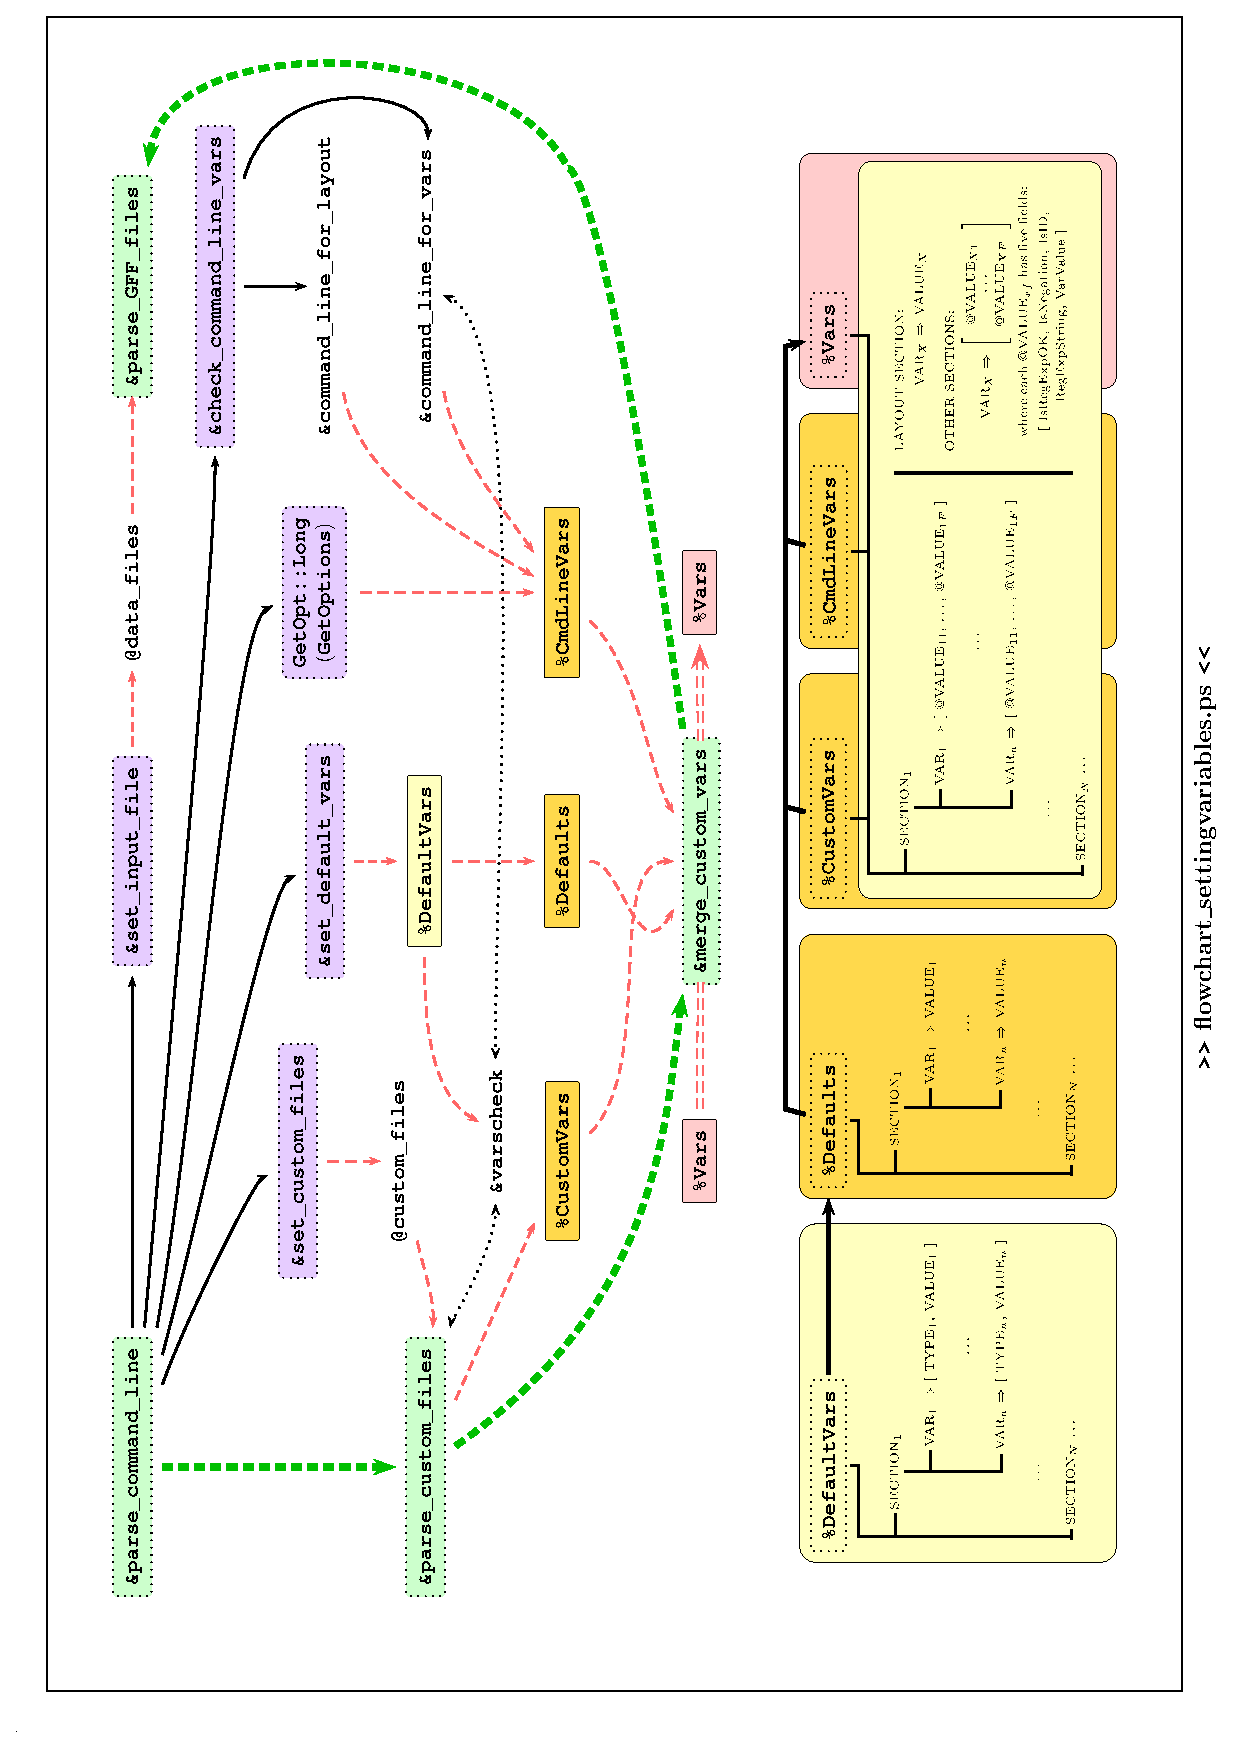
\includegraphics[bb=20 5 540 770,clip,angle=270,width=\linewidth]
                 {./psfigures/flowchart_settingvariables.ps}
}%fbox
\caption[Structure of main customization variables]{\label{fig:customvarstruc} Data structure schemma of main customization variables and their relationships: {\tt{}{\char37}DefaultVars}, {\tt{}{\char37}CmdLineVars}, {\tt{}{\char37}CustomVars}, {\tt{}{\char37}Defaults}, {\tt{}{\char37}Vars}. Last three variables share the same internal data structure. Above them, a graph showing the processes involved in the parsing of customization parameters from different sources (defaults, customization file and command-line) and the functions involved in the definition of those variables. Green arrow and boxes correspond to main loop functions, which are also executed in that order.}
\end{center}
\end{figure}

\subsctn{Setting customization parameters from defaults} 

The main difference from older versions, besides a cleaner hash structure than the GAWK one, is that we include some customization variables at sequence and strand levels. Almost all the variables are described in section~\ref{sec:customvardesc}, page~\pageref{sec:customvardesc}.

\nwenddocs{}\nwbegincode{51}\sublabel{NWgff18-SetG-1}\nwmargintag{{\nwtagstyle{}\subpageref{NWgff18-SetG-1}}}\moddef{Setting Defaults~{\nwtagstyle{}\subpageref{NWgff18-SetG-1}}}\endmoddef
sub set_default_vars() \{
    %DefaultVars = (
        LAYOUT   => \{           ## '# L #'
            \LA{}default layout vars values~{\nwtagstyle{}\subpageref{NWgff18-defQ-1}}\RA{}
        \},                    
        SEQUENCE => \{           ## '# Q #'
            \LA{}default sequence vars values~{\nwtagstyle{}\subpageref{NWgff18-defS-1}}\RA{}
        \},                    
        SOURCE   => \{           ## '# S #'
            \LA{}default source vars values~{\nwtagstyle{}\subpageref{NWgff18-defQ.2-1}}\RA{}
        \},                    
        STRAND   => \{           ## '# T #'
            \LA{}default strand vars values~{\nwtagstyle{}\subpageref{NWgff18-defQ.3-1}}\RA{}
        \},                    
        GROUP    => \{           ## '# G #'
            \LA{}default group vars values~{\nwtagstyle{}\subpageref{NWgff18-defP-1}}\RA{}
        \},                    
        FEATURE  => \{           ## '# F #'
            \LA{}default feature vars values~{\nwtagstyle{}\subpageref{NWgff18-defR-1}}\RA{}
        \},
    ); # %DefaultVars
    \LA{}map default vars to defaults working copy~{\nwtagstyle{}\subpageref{NWgff18-mapf-1}}\RA{}
    print LOGFILE (Data::Dumper->Dump([ \\%DefaultVars ],
                                   [ qw( *DefaultVars ) ]))
        if ($LogFile && $Debug);
\} # set_default_vars
\nosublabel{NWgff18-SetG-1-u7}\nwindexdefn{{\char38}set{\char95}default{\char95}vars}{:amset:undefault:unvars}{NWgff18-SetG-1}\eatline
\nwidentdefs{\\{{{\char38}set{\char95}default{\char95}vars}{:amset:undefault:unvars}}}\nwused{\\{NWgff18-MaiD-1}}\nwendcode{}\nwbegindocs{52}% print LOGFILE '>>> %DefaultVars : '.(Dumper(\%DefaultVars))

We also build from this structure, making easier variable maintenance because default value and variable type are edited together in {\tt{}{\char37}DefaultVars} (as {\tt{}TYPE}/{\tt{}VALUE} pairs), an auxiliary variable which allows us to load default values into GFF elements.

\label{sec:tmpdefaults}
\nwenddocs{}\nwbegincode{53}\sublabel{NWgff18-mapf-1}\nwmargintag{{\nwtagstyle{}\subpageref{NWgff18-mapf-1}}}\moddef{map default vars to defaults working copy~{\nwtagstyle{}\subpageref{NWgff18-mapf-1}}}\endmoddef
%Defaults = ();
foreach my $sct (keys %DefaultVars) \{
    foreach my $vnm (keys %\{$DefaultVars\{$sct\}\}) \{
        $Defaults\{$sct\}\{$vnm\} = $DefaultVars\{$sct\}\{$vnm\}\{'VALUE'\};
    \}; # foreach $vnm
\}; # foreach $sct
\nwused{\\{NWgff18-SetG-1}}\nwendcode{}\nwbegindocs{54}\nwdocspar

\subsubsctn{Default customization files}

\nwenddocs{}\nwbegincode{55}\sublabel{NWgff18-GloB-1}\nwmargintag{{\nwtagstyle{}\subpageref{NWgff18-GloB-1}}}\moddef{Global Vars~{\nwtagstyle{}\subpageref{NWgff18-GloB-1}}}\endmoddef
my $Custom_path = defined($ENV\{GFF2APLOT_CUSTOMPATH\})
                  ? $ENV\{GFF2APLOT_CUSTOMPATH\} : '.';
my $Custom_file = defined($ENV\{GFF2APLOT_CUSTOMFILE\})
                  ? $ENV\{GFF2APLOT_CUSTOMFILE\} : '.gff2aplotrc';
$Custom_path =~ s\{/$\}\{\}o; 
\nwalsodefined{\\{NWgff18-GloB-2}\\{NWgff18-GloB-3}\\{NWgff18-GloB-4}\\{NWgff18-GloB-5}\\{NWgff18-GloB-6}\\{NWgff18-GloB-7}\\{NWgff18-GloB-8}\\{NWgff18-GloB-9}\\{NWgff18-GloB-A}\\{NWgff18-GloB-B}\\{NWgff18-GloB-C}\\{NWgff18-GloB-D}\\{NWgff18-GloB-E}\\{NWgff18-GloB-F}\\{NWgff18-GloB-G}\\{NWgff18-GloB-H}\\{NWgff18-GloB-I}\\{NWgff18-GloB-J}\\{NWgff18-GloB-K}\\{NWgff18-GloB-L}\\{NWgff18-GloB-M}\\{NWgff18-GloB-N}}\nwused{\\{NWgff18-APL5-1}}\nwendcode{}\nwbegindocs{56}\nwdocspar

We remove any trailing '{\tt{}/}' from '{\tt{}{\char36}Custom{\char95}path}' that user could have introduced to avoid any problem with full custom filenames later.

\nwenddocs{}\nwbegincode{57}\sublabel{NWgff18-envL-1}\nwmargintag{{\nwtagstyle{}\subpageref{NWgff18-envL-1}}}\moddef{environment vars help~{\nwtagstyle{}\subpageref{NWgff18-envL-1}}}\endmoddef
    There are two environmental variables that can be set by 
users to their preferences:
 + You can specify the path where $PROGRAM can find the default
  files with the shell variable \\"GFF2APLOT_CUSTOMPATH\\". Default
  value is the path where you are running $PROGRAM.
 + You can also define the default custom filename you will like
  with the variable \\"GFF2APLOT_CUSTOMFILE\\", program default
  filename for custom file is \\".gff2aplotrc\\".
 + Now $PROGRAM does not need to write any temporary file, 
  so that previous versions default temporary directory path
  variable (\\"GFF2APLOT_TMP\\") is no longer used.
 + Setting those vars in Bourne-shell and C-shell:
   o Using a Bourne-Shell (e.g. bash):
        export GFF2APLOT_CUSTOMPATH=\\"path\\"
        export GFF2APLOT_CUSTOMFILE=\\"file_name\\"
   o Using a C-Shell:
        setenv GFF2APLOT_CUSTOMPATH \\"path\\"
        setenv GFF2APLOT_CUSTOMFILE \\"file_name\\"
\nwused{\\{NWgff18-MaiD-2}}\nwendcode{}\nwbegindocs{58}%$


\subsctn{Setting customization parameters from command-line} 

'{\tt{}GetOptions}' loads command-line options as key-value pairs in the hash variable '{\tt{}{\char37}CmdLineVars}' 
that is reset in '{\tt{}\LA{}Main Loop~{\nwtagstyle{}\subpageref{NWgff18-Mai9-1}}\RA{}}'. Once parsed all the command-line options what remains in '{\tt{}@ARGV}' is just input filenames (which have to be in GFF format), or '{\tt{}STDIN}' if there is none.

\nwenddocs{}\nwbegincode{59}\sublabel{NWgff18-ParS-1}\nwmargintag{{\nwtagstyle{}\subpageref{NWgff18-ParS-1}}}\moddef{Parsing Command-Line Options~{\nwtagstyle{}\subpageref{NWgff18-ParS-1}}}\endmoddef
sub parse_command_line() \{
    \LA{}looking for STDIN~{\nwtagstyle{}\subpageref{NWgff18-looH-1}}\RA{}

    $SIG\{__WARN__\} = sub \{ &warn('UNKNOWN_CL_OPTION',$T,$_[0]) \};
    GetOptions(
               \LA{}command-line options prog~{\nwtagstyle{}\subpageref{NWgff18-comP-1}}\RA{}
               \LA{}command-line options~{\nwtagstyle{}\subpageref{NWgff18-comK-1}}\RA{}
               \LA{}command-line options custom~{\nwtagstyle{}\subpageref{NWgff18-comR-1}}\RA{}
               \LA{}command-line options with exit~{\nwtagstyle{}\subpageref{NWgff18-comU-1}}\RA{}
               ) || (&warn('CMD_LINE_ERROR',$T), exit(1));
    $SIG\{__WARN__\} = 'DEFAULT';

    \LA{}open LOGFILE~{\nwtagstyle{}\subpageref{NWgff18-opeC-1}}\RA{}

    &header('',"RUNNING $PROGRAM",'',"User: $USER","Date: $DATE","Perl: $PVER");

    &header("SETTING DEFAULTS");
    %DefaultVars = ();
    &set_default_vars;

    &header("CHECKING COMMAND-LINE OPTIONS");
    @data_files = ();
    &set_input_file($cmdln_stdin);
    @ARGV = (); # ensuring that command-line ARGVs array is empty

    &set_custom_files();

    &check_command_line_vars();

    &footer("COMMAND-LINE CHECKED");
\} # parse_command_line
\nwindexdefn{{\char38}parse{\char95}command{\char95}line}{:amparse:uncommand:unline}{NWgff18-ParS-1}\eatline
\nwidentdefs{\\{{{\char38}parse{\char95}command{\char95}line}{:amparse:uncommand:unline}}}\nwidentuses{\\{{{\char38}check{\char95}command{\char95}line{\char95}vars}{:amcheck:uncommand:unline:unvars}}\\{{{\char38}footer}{:amfooter}}\\{{{\char38}header}{:amheader}}\\{{line}{line}}\\{{{\char38}set{\char95}custom{\char95}files}{:amset:uncustom:unfiles}}\\{{{\char38}set{\char95}default{\char95}vars}{:amset:undefault:unvars}}\\{{{\char38}set{\char95}input{\char95}file}{:amset:uninput:unfile}}\\{{{\char38}warn}{:amwarn}}}\nwindexuse{{\char38}check{\char95}command{\char95}line{\char95}vars}{:amcheck:uncommand:unline:unvars}{NWgff18-ParS-1}\nwindexuse{{\char38}footer}{:amfooter}{NWgff18-ParS-1}\nwindexuse{{\char38}header}{:amheader}{NWgff18-ParS-1}\nwindexuse{line}{line}{NWgff18-ParS-1}\nwindexuse{{\char38}set{\char95}custom{\char95}files}{:amset:uncustom:unfiles}{NWgff18-ParS-1}\nwindexuse{{\char38}set{\char95}default{\char95}vars}{:amset:undefault:unvars}{NWgff18-ParS-1}\nwindexuse{{\char38}set{\char95}input{\char95}file}{:amset:uninput:unfile}{NWgff18-ParS-1}\nwindexuse{{\char38}warn}{:amwarn}{NWgff18-ParS-1}\nwalsodefined{\\{NWgff18-ParS-2}\\{NWgff18-ParS-3}\\{NWgff18-ParS-4}\\{NWgff18-ParS-5}\\{NWgff18-ParS-6}}\nwused{\\{NWgff18-MaiD-1}}\nwendcode{}\nwbegindocs{60}\nwdocspar
As the '{\tt{}GetOptions}' function has a problem, in the way we are using here to preserve backwards compatibility, when we want to use a single dash as a way to tell the program that '{\tt{}STDIN}' must be read in the given order (when input filenames are also given and we would load input from a pipe after/before a given file). We show the warnings printed by the program when '{\tt{}--}' is missing or missplaced in the table~\ref{tbl:STDINhandle}.

\begin{table}[!t]
\begin{center}
\begin{small}
\begin{tabular}{|c|}\hline
\begin{minipage}{15cm}
\begin{verbatim}

# CORRECT
> $BIN/gff2aplot -v -T 'Howdy World!' -- - DATA-SAMPLE.gff 
> $BIN/gff2aplot -v -T 'Howdy World!' -- DATA-SAMPLE.gff -

# WRONG???
> $BIN/gff2aplot -v -T 'Howdy World!' DATA-SAMPLE.gff -
> $BIN/gff2aplot -v -T 'Howdy World!' - DATA-SAMPLE.gff
> $BIN/gff2aplot -v -T 'Howdy World!' - -- tests/DATA-SAMPLE.gff

# COMMON MESSAGE when WRONG
### WARNING ### Error trapped while processing command-line:
                substr outside of string at lib/Getopt/Long.pm
                  (autosplit into lib/auto/Getopt/Long/FindOption.al)
                line >NNNNN<
### WARNING ### Error trapped while processing command-line:
                Use of uninitialized value at lib/Getopt/Long.pm
                  (autosplit into lib/auto/Getopt/Long/FindOption.al) 
                line >NNNNN<
### WARNING ### Error trapped while processing command-line:
                Unknown option:

\end{verbatim}
% $
\end{minipage}\\\hline
\end{tabular}
\end{small}
\caption[Fixing {\tt{}GetOptions} for using '{\tt{}-}' as '{\tt{}STDIN}' mark.]{\label{tbl:STDINhandle} Errors reported when using '{\tt{}-}' as '{\tt{}STDIN}' mark and fixed width {\tt{}\LA{}looking for STDIN~{\nwtagstyle{}\subpageref{NWgff18-looH-1}}\RA{}}.}
\end{center}
\end{table}

To avoid such errors, we capture the single dash when present in the command-line arguments list. 

'{\tt{}{\char36}cmdln{\char95}stdin}' will be used by '{\tt{}\protect\nwindexuse{{\char38}set{\char95}input{\char95}file}{:amset:uninput:unfile}{NWgff18-ParS-3}{\char38}set{\char95}input{\char95}file}' function to include the '{\tt{}STDIN}' in the correct ordering.\label{sec:stdinfix}

\nwenddocs{}\nwbegincode{61}\sublabel{NWgff18-looH-1}\nwmargintag{{\nwtagstyle{}\subpageref{NWgff18-looH-1}}}\moddef{looking for STDIN~{\nwtagstyle{}\subpageref{NWgff18-looH-1}}}\endmoddef
my $cmdln_stdin = undef;
for (my $a = 0; $a <= $#ARGV; $a++) \{ 
    next unless $ARGV[$a] =~ /^-$/o;
    $cmdln_stdin = $a - $#ARGV;
    splice(@ARGV,$a,1);
\};    
\nwused{\\{NWgff18-ParS-1}}\nwendcode{}\nwbegindocs{62}\nwdocspar

The following two code chunks define what to do if reports are sent to a file which is set in '{\tt{}{\char36}logs{\char95}filename}'.

\nwenddocs{}\nwbegincode{63}\sublabel{NWgff18-opeC-1}\nwmargintag{{\nwtagstyle{}\subpageref{NWgff18-opeC-1}}}\moddef{open LOGFILE~{\nwtagstyle{}\subpageref{NWgff18-opeC-1}}}\endmoddef
CHKLOG:
  (defined($logs_filename)) && do \{
      open(LOGFILE,"> ".$logs_filename) ||
          (&warn('FILE_NO_OPEN',$T,$logs_filename),last CHKLOG);
      $LogFile = 1;
  \};
\nwidentuses{\\{{{\char38}warn}{:amwarn}}}\nwindexuse{{\char38}warn}{:amwarn}{NWgff18-opeC-1}\nwused{\\{NWgff18-ParS-1}}\nwendcode{}\nwbegindocs{64}\nwdocspar

\nwenddocs{}\nwbegincode{65}\sublabel{NWgff18-ComF-1}\nwmargintag{{\nwtagstyle{}\subpageref{NWgff18-ComF-1}}}\moddef{Common Routines~{\nwtagstyle{}\subpageref{NWgff18-ComF-1}}}\endmoddef
sub close_logfile() \{ close(LOGFILE) if $LogFile \};
\nwindexdefn{{\char38}close{\char95}logfile}{:amclose:unlogfile}{NWgff18-ComF-1}\eatline
\nwidentdefs{\\{{{\char38}close{\char95}logfile}{:amclose:unlogfile}}}\nwalsodefined{\\{NWgff18-ComF-2}\\{NWgff18-ComF-3}\\{NWgff18-ComF-4}\\{NWgff18-ComF-5}\\{NWgff18-ComF-6}\\{NWgff18-ComF-7}\\{NWgff18-ComF-8}\\{NWgff18-ComF-9}\\{NWgff18-ComF-A}\\{NWgff18-ComF-B}\\{NWgff18-ComF-C}\\{NWgff18-ComF-D}}\nwused{\\{NWgff18-APL5-1}}\nwendcode{}\nwbegindocs{66}\nwdocspar
\nwenddocs{}\nwbegincode{67}\sublabel{NWgff18-UseB-2}\nwmargintag{{\nwtagstyle{}\subpageref{NWgff18-UseB-2}}}\moddef{Use Modules~{\nwtagstyle{}\subpageref{NWgff18-UseB-1}}}\plusendmoddef
use Getopt::Long;
Getopt::Long::Configure qw/ bundling /;
\nwendcode{}\nwbegindocs{68}\nwdocspar

\nwenddocs{}\nwbegincode{69}\sublabel{NWgff18-perI-2}\nwmargintag{{\nwtagstyle{}\subpageref{NWgff18-perI-2}}}\moddef{perl requires help~{\nwtagstyle{}\subpageref{NWgff18-perI-1}}}\plusendmoddef
"Getopt::Long" - processing command-line options.
\nwidentuses{\\{{line}{line}}}\nwindexuse{line}{line}{NWgff18-perI-2}\nwendcode{}\nwbegindocs{70}\nwdocspar

See '{\tt{}man\ Getopt::Long}' for further info about this package.

\nwenddocs{}\nwbegincode{71}\sublabel{NWgff18-GloB-2}\nwmargintag{{\nwtagstyle{}\subpageref{NWgff18-GloB-2}}}\moddef{Global Vars~{\nwtagstyle{}\subpageref{NWgff18-GloB-1}}}\plusendmoddef
my ($Debug,$Verbose,$Quiet,$LogFile,$logs_filename) = ($F,$F,$F,$F,undef);
\nwendcode{}\nwbegindocs{72}\nwdocspar

\nwenddocs{}\nwbegincode{73}\sublabel{NWgff18-ward-1}\nwmargintag{{\nwtagstyle{}\subpageref{NWgff18-ward-1}}}\moddef{warnings - parsing command-line options~{\nwtagstyle{}\subpageref{NWgff18-ward-1}}}\endmoddef
UNKNOWN_CL_OPTION =>
  $Warn."Error trapped while processing command-line:\\n".(" "x16)."\\%s\\n",
CMD_LINE_ERROR =>
  $spl.$spw." Please, check your command-line options!!!\\n".$Error."\\n".
  $spw." ".("."x12)." Type \\"$PROGRAM -h\\" for help.\\n".$spl,
\nwidentuses{\\{{line}{line}}}\nwindexuse{line}{line}{NWgff18-ward-1}\nwused{\\{NWgff18-GloB-M}}\nwendcode{}\nwbegindocs{74}\nwdocspar

\subsubsctn{Special command-line options (forcing exit from program)}

The first command-line checking looks for those options exiting the program: '{\tt{}help}' and '{\tt{}version}'. Both need to output to screen without any other message/warning being displayed at the same time.

\nwenddocs{}\nwbegincode{75}\sublabel{NWgff18-comU-1}\nwmargintag{{\nwtagstyle{}\subpageref{NWgff18-comU-1}}}\moddef{command-line options with exit~{\nwtagstyle{}\subpageref{NWgff18-comU-1}}}\endmoddef
"version"   => \\&prt_version, 
"h|help|?"  => \\&prt_help,
\nwidentuses{\\{{{\char38}prt{\char95}help}{:amprt:unhelp}}\\{{{\char38}prt{\char95}version}{:amprt:unversion}}}\nwindexuse{{\char38}prt{\char95}help}{:amprt:unhelp}{NWgff18-comU-1}\nwindexuse{{\char38}prt{\char95}version}{:amprt:unversion}{NWgff18-comU-1}\nwused{\\{NWgff18-ParS-1}}\nwendcode{}\nwbegindocs{76}\nwdocspar
\nwenddocs{}\nwbegincode{77}\sublabel{NWgff18-comM-1}\nwmargintag{{\nwtagstyle{}\subpageref{NWgff18-comM-1}}}\moddef{command-line help prog~{\nwtagstyle{}\subpageref{NWgff18-comM-1}}}\endmoddef
-h, --help   Shows this help.
--version    Shows current version and exits.
\nwalsodefined{\\{NWgff18-comM-2}\\{NWgff18-comM-3}\\{NWgff18-comM-4}}\nwused{\\{NWgff18-comH-1}}\nwendcode{}\nwbegindocs{78}\nwdocspar
\nwenddocs{}\nwbegincode{79}\sublabel{NWgff18-DESP-1}\nwmargintag{{\nwtagstyle{}\subpageref{NWgff18-DESP-1}}}\moddef{DESC command-line options~{\nwtagstyle{}\subpageref{NWgff18-DESP-1}}}\endmoddef
ORD: 1
OPT: h
LNG: help
SDE: Showing the command-line help (and exit).
LDE:
Shows command-line help.
###EOR###
ORD: 2
LNG: version
SDE: Shows current version and exits from program.
LDE:
Shows current program version and exits.
###EOR###
\nwidentuses{\\{{line}{line}}}\nwindexuse{line}{line}{NWgff18-DESP-1}\nwalsodefined{\\{NWgff18-DESP-2}\\{NWgff18-DESP-3}\\{NWgff18-DESP-4}\\{NWgff18-DESP-5}\\{NWgff18-DESP-6}\\{NWgff18-DESP-7}\\{NWgff18-DESP-8}\\{NWgff18-DESP-9}\\{NWgff18-DESP-A}\\{NWgff18-DESP-B}\\{NWgff18-DESP-C}\\{NWgff18-DESP-D}\\{NWgff18-DESP-E}\\{NWgff18-DESP-F}\\{NWgff18-DESP-G}\\{NWgff18-DESP-H}\\{NWgff18-DESP-I}\\{NWgff18-DESP-J}\\{NWgff18-DESP-K}\\{NWgff18-DESP-L}\\{NWgff18-DESP-M}\\{NWgff18-DESP-N}\\{NWgff18-DESP-O}\\{NWgff18-DESP-P}\\{NWgff18-DESP-Q}\\{NWgff18-DESP-R}\\{NWgff18-DESP-S}\\{NWgff18-DESP-T}\\{NWgff18-DESP-U}\\{NWgff18-DESP-V}\\{NWgff18-DESP-W}}\nwnotused{DESC\ command-line\ options}\nwendcode{}\nwbegindocs{80}\nwdocspar


\nwenddocs{}\nwbegincode{81}\sublabel{NWgff18-ParS-2}\nwmargintag{{\nwtagstyle{}\subpageref{NWgff18-ParS-2}}}\moddef{Parsing Command-Line Options~{\nwtagstyle{}\subpageref{NWgff18-ParS-1}}}\plusendmoddef
sub prt_version() \{
    my $comment = $Messages\{'SHOW_VERSION'\};
    $comment = sprintf($comment,$PROGRAM,$VERSION);
    &prt_to_stderr($comment);
    exit(1);
\} # prt_version
\nwindexdefn{{\char38}prt{\char95}version}{:amprt:unversion}{NWgff18-ParS-2}\eatline
\nwidentdefs{\\{{{\char38}prt{\char95}version}{:amprt:unversion}}}\nwidentuses{\\{{{\char38}prt{\char95}to{\char95}stderr}{:amprt:unto:unstderr}}}\nwindexuse{{\char38}prt{\char95}to{\char95}stderr}{:amprt:unto:unstderr}{NWgff18-ParS-2}\nwendcode{}\nwbegindocs{82}\nwdocspar
\nwenddocs{}\nwbegincode{83}\sublabel{NWgff18-mesd-1}\nwmargintag{{\nwtagstyle{}\subpageref{NWgff18-mesd-1}}}\moddef{messages - parsing command-line options~{\nwtagstyle{}\subpageref{NWgff18-mesd-1}}}\endmoddef
SHOW_VERSION =>
  $sp."### \\%s -- \\%s\\n".$sp,
\nwused{\\{NWgff18-GloB-M}}\nwendcode{}\nwbegindocs{84}\nwdocspar

\subsubsctn{Testing command-line input filenames}

\nwenddocs{}\nwbegincode{85}\sublabel{NWgff18-ParS-3}\nwmargintag{{\nwtagstyle{}\subpageref{NWgff18-ParS-3}}}\moddef{Parsing Command-Line Options~{\nwtagstyle{}\subpageref{NWgff18-ParS-1}}}\plusendmoddef
sub set_input_file() \{
    my $stdin_flg = $F;
    \LA{}STDIN backwards compatibility~{\nwtagstyle{}\subpageref{NWgff18-STDT-1}}\RA{}
    &report("CHECKING_FILENAMES");
  FILECHK: foreach my $test_file (@ARGV) \{
        $test_file ne '-' && do \{
            -e $test_file || do \{
                &warn('FILE_NO_OPEN',$T,$test_file);
                next FILECHK;
            \};
            &report('READING_FILE',$test_file);
            push @data_files, $test_file;
            next FILECHK;
        \};
        $stdin_flg = $T;
        push @data_files, '-';
    \}; # foreach
    scalar(@data_files) == 0 && do \{
        push @data_files, '-';
        $stdin_flg = $T;
    \};
    $stdin_flg && &report('READING_STDIN');
\} # set_input_file
\nwindexdefn{{\char38}set{\char95}input{\char95}file}{:amset:uninput:unfile}{NWgff18-ParS-3}\eatline
\nwidentdefs{\\{{{\char38}set{\char95}input{\char95}file}{:amset:uninput:unfile}}}\nwidentuses{\\{{{\char38}report}{:amreport}}\\{{{\char38}warn}{:amwarn}}}\nwindexuse{{\char38}report}{:amreport}{NWgff18-ParS-3}\nwindexuse{{\char38}warn}{:amwarn}{NWgff18-ParS-3}\nwendcode{}\nwbegindocs{86}\nwdocspar
\nwenddocs{}\nwbegincode{87}\sublabel{NWgff18-GloB-3}\nwmargintag{{\nwtagstyle{}\subpageref{NWgff18-GloB-3}}}\moddef{Global Vars~{\nwtagstyle{}\subpageref{NWgff18-GloB-1}}}\plusendmoddef
my (@data_files,$file);
\nwendcode{}\nwbegindocs{88}\nwdocspar

\nwenddocs{}\nwbegincode{89}\sublabel{NWgff18-outN-1}\nwmargintag{{\nwtagstyle{}\subpageref{NWgff18-outN-1}}}\moddef{warnings - input/output~{\nwtagstyle{}\subpageref{NWgff18-outN-1}}}\endmoddef
FILE_NO_OPEN =>
  $spl.$Warn."Cannot Open Current file \\"\\%s\\" . Not used !!!\\n".$spl,
\nwalsodefined{\\{NWgff18-outN-2}}\nwused{\\{NWgff18-GloB-M}}\nwendcode{}\nwbegindocs{90}\nwdocspar

\nwenddocs{}\nwbegincode{91}\sublabel{NWgff18-outN.2-1}\nwmargintag{{\nwtagstyle{}\subpageref{NWgff18-outN.2-1}}}\moddef{messages - input/output~{\nwtagstyle{}\subpageref{NWgff18-outN.2-1}}}\endmoddef
CHECKING_FILENAMES =>
  $sp."### Validating INPUT FILENAMES\\n".$sp,
READING_FILE =>
  "###---> \\"\\%s\\" exists, including as Input File.\\n",
READING_STDIN =>
  "###---> Including GFF records from standard input.\\n",  
\nwalsodefined{\\{NWgff18-outN.2-2}\\{NWgff18-outN.2-3}\\{NWgff18-outN.2-4}\\{NWgff18-outN.2-5}\\{NWgff18-outN.2-6}\\{NWgff18-outN.2-7}\\{NWgff18-outN.2-8}\\{NWgff18-outN.2-9}\\{NWgff18-outN.2-A}\\{NWgff18-outN.2-B}\\{NWgff18-outN.2-C}\\{NWgff18-outN.2-D}\\{NWgff18-outN.2-E}\\{NWgff18-outN.2-F}\\{NWgff18-outN.2-G}\\{NWgff18-outN.2-H}}\nwused{\\{NWgff18-GloB-M}}\nwendcode{}\nwbegindocs{92}\nwdocspar

Here is the fix for the explained in section~\ref{sec:stdinfix} on page~\pageref{sec:stdinfix} ({\tt{}\LA{}looking for STDIN~{\nwtagstyle{}\subpageref{NWgff18-looH-1}}\RA{}} code).

\nwenddocs{}\nwbegincode{93}\sublabel{NWgff18-STDT-1}\nwmargintag{{\nwtagstyle{}\subpageref{NWgff18-STDT-1}}}\moddef{STDIN backwards compatibility~{\nwtagstyle{}\subpageref{NWgff18-STDT-1}}}\endmoddef
my $chk_stdin = shift @_;
my $t = scalar(@ARGV);
defined($chk_stdin) && do \{
    abs($chk_stdin) > $t && ($chk_stdin = -$t);
    $chk_stdin > 0  && ($chk_stdin = 0 );
    $t += $chk_stdin;
    splice(@ARGV,$t,0,'-');
\};
\nwused{\\{NWgff18-ParS-3}}\nwendcode{}\nwbegindocs{94}\nwdocspar

\subsubsctn{Verifying command-line settings}

\nwenddocs{}%
%
\nwbegindocs{96}\nwdocspar

As we reset {\tt{}{\char37}CmdLineVars} in main loop we do not need to take care for those key-value pairs that were not defined by {\tt{}GetOptions} function. We will check for two kinds of command-line variables, those having a specific command-line option (and related to {\tt{}LAYOUT} variables) and those that define a feature-specific variable (for GFF-features, groups, sequences and so on). Last ones are validated and set in the following section. Therefore, if layout variables are provided on command-line by this way, they have precedence over the corresponding layout pre-defined command-line option. 

\nwenddocs{}\nwbegincode{97}\sublabel{NWgff18-ParS-4}\nwmargintag{{\nwtagstyle{}\subpageref{NWgff18-ParS-4}}}\moddef{Parsing Command-Line Options~{\nwtagstyle{}\subpageref{NWgff18-ParS-1}}}\plusendmoddef
sub check_command_line_vars() \{
    &report("CHECKING_CMDLN_OPTS");
    &command_line_for_layout();
    defined($CmdLineVars\{VARS\}) &&
        &report("CHECKING_CMDLN_VARS");
        &command_line_for_vars();
    &footer("COMMAND-LINE OPTIONS CHECKED");
\} # check_command_line_vars
\nwindexdefn{{\char38}check{\char95}command{\char95}line{\char95}vars}{:amcheck:uncommand:unline:unvars}{NWgff18-ParS-4}\eatline
\nwidentdefs{\\{{{\char38}check{\char95}command{\char95}line{\char95}vars}{:amcheck:uncommand:unline:unvars}}}\nwidentuses{\\{{{\char38}command{\char95}line{\char95}for{\char95}layout}{:amcommand:unline:unfor:unlayout}}\\{{{\char38}command{\char95}line{\char95}for{\char95}vars}{:amcommand:unline:unfor:unvars}}\\{{{\char38}footer}{:amfooter}}\\{{{\char38}report}{:amreport}}}\nwindexuse{{\char38}command{\char95}line{\char95}for{\char95}layout}{:amcommand:unline:unfor:unlayout}{NWgff18-ParS-4}\nwindexuse{{\char38}command{\char95}line{\char95}for{\char95}vars}{:amcommand:unline:unfor:unvars}{NWgff18-ParS-4}\nwindexuse{{\char38}footer}{:amfooter}{NWgff18-ParS-4}\nwindexuse{{\char38}report}{:amreport}{NWgff18-ParS-4}\nwendcode{}\nwbegindocs{98}\nwdocspar
\nwenddocs{}\nwbegincode{99}\sublabel{NWgff18-outN.2-2}\nwmargintag{{\nwtagstyle{}\subpageref{NWgff18-outN.2-2}}}\moddef{messages - input/output~{\nwtagstyle{}\subpageref{NWgff18-outN.2-1}}}\plusendmoddef
CHECKING_CMDLN_OPTS =>
  $sp."### Checking COMMAND-LINE Options\\n".$sp,
CHECKING_CMDLN_VARS =>
  $sp."### Checking Custom Variables SET by COMMAND-LINE\\n".$sp,
\nwendcode{}\nwbegindocs{100}\nwdocspar

Here we take advantage of the {\tt{}\protect\nwindexuse{{\char38}varscheck}{:amvarscheck}{NWgff18-ParK-3}{\char38}varscheck} function, that was created to validate input from {\tt{}\protect\nwindexuse{{\char38}parse{\char95}custom{\char95}files}{:amparse:uncustom:unfiles}{NWgff18-ParK-2}{\char38}parse{\char95}custom{\char95}files}, and that is described in section~\ref{sec:paramvalid}, page~\pageref{sec:paramvalid}.

\nwenddocs{}\nwbegincode{101}\sublabel{NWgff18-ParS-5}\nwmargintag{{\nwtagstyle{}\subpageref{NWgff18-ParS-5}}}\moddef{Parsing Command-Line Options~{\nwtagstyle{}\subpageref{NWgff18-ParS-1}}}\plusendmoddef
sub command_line_for_layout() \{
    ($n,$c) = (0, '');
    foreach my $cvar (keys %\{ $CmdLineVars\{LAYOUT\} \}) \{
        defined($CmdLineVars\{LAYOUT\}\{$cvar\}) && do \{
            my @cary = ('LAYOUT',$cvar,$CmdLineVars\{LAYOUT\}\{$cvar\});
            $c = &varscheck($F,'LAYOUT',\\@cary,\\%CmdLineVars) ? '.' : $noCV;
            &counter(++$n,$c);
        \}; # defined($CmdLineVars\{LAYOUT\}\{$cvar\})
    \}; # foreach $cvar
    &counter_end($n,$c);
    print LOGFILE (Data::Dumper->Dump([ \\%\{ $CmdLineVars\{LAYOUT\} \} ],
                                    [ qw( *\{$CmdLineVars\{LAYOUT\}\} ) ]))
        if ($LogFile && $Debug);
\} # command_line_for_layout
\nwindexdefn{{\char38}command{\char95}line{\char95}for{\char95}layout}{:amcommand:unline:unfor:unlayout}{NWgff18-ParS-5}\eatline
\nwidentdefs{\\{{{\char38}command{\char95}line{\char95}for{\char95}layout}{:amcommand:unline:unfor:unlayout}}}\nwidentuses{\\{{{\char38}varscheck}{:amvarscheck}}}\nwindexuse{{\char38}varscheck}{:amvarscheck}{NWgff18-ParS-5}\nwendcode{}\nwbegindocs{102}\nwdocspar
\subsubsctn{Loading GFF elements custom variables from command-line}

\nwenddocs{}%
%
%
%
%
\nwbegindocs{104}\nwdocspar

\nwenddocs{}\nwbegincode{105}\sublabel{NWgff18-ParS-6}\nwmargintag{{\nwtagstyle{}\subpageref{NWgff18-ParS-6}}}\moddef{Parsing Command-Line Options~{\nwtagstyle{}\subpageref{NWgff18-ParS-1}}}\plusendmoddef
sub command_line_for_vars() \{
    ($n,$c) = (0, '');
    foreach my $calias ( qw/ L Q S T G F / ) \{
        my ($cvar,$cflg);
        $cvar = $VarKeys\{$calias\};
        $cflg = ($calias ne 'L') ? $T : $F;
        defined($CmdLineVars\{VARS\}\{$cvar\}) && do \{
            foreach my $ccv (@\{ $CmdLineVars\{VARS\}\{$cvar\} \}) \{
                my @clin = ();
              TWOTHREE: \{
                  $cflg && do \{
                      $ccv =~ /^(.*?):\{2\}(.*?)=\{1\}(.*?)$/o &&
                              (@clin = ($1,$2,$3));
                      last TWOTHREE;
                  \};
                  $ccv =~ /^(.*?)=\{1\}(.*?)$/o && (@clin = ($cvar,$1,$2));
                \}; # TWOTHREE
                $c = &varscheck($cflg,$cvar,\\@clin,\\%CmdLineVars)
                     ? $calias : $noCV;
                &counter(++$n,$c);
            \}; # foreach $ccv
        \}; # $CmdLineVars\{VARS\}\{$cvar\}
    \}; # foreach $calias
    &counter_end($n,$c);
    print LOGFILE (Data::Dumper->Dump([ \\%\{ $CmdLineVars\{VARS\} \} ],
                                    [ qw( *\{$CmdLineVars\{VARS\}\} ) ]))
        if ($LogFile && $Debug);
\} # command_line_for_vars
\nwindexdefn{{\char38}command{\char95}line{\char95}for{\char95}vars}{:amcommand:unline:unfor:unvars}{NWgff18-ParS-6}\eatline
\nwidentdefs{\\{{{\char38}command{\char95}line{\char95}for{\char95}vars}{:amcommand:unline:unfor:unvars}}}\nwidentuses{\\{{{\char38}varscheck}{:amvarscheck}}}\nwindexuse{{\char38}varscheck}{:amvarscheck}{NWgff18-ParS-6}\nwendcode{}\nwbegindocs{106}\nwdocspar
\nwenddocs{}\nwbegincode{107}\sublabel{NWgff18-comR-1}\nwmargintag{{\nwtagstyle{}\subpageref{NWgff18-comR-1}}}\moddef{command-line options custom~{\nwtagstyle{}\subpageref{NWgff18-comR-1}}}\endmoddef
"layout-var=s@"   => \\@\{ $CmdLineVars\{VARS\}\{LAYOUT\} \},
"sequence-var=s@" => \\@\{ $CmdLineVars\{VARS\}\{SEQUENCE\} \},
"source-var=s@"   => \\@\{ $CmdLineVars\{VARS\}\{SOURCE\} \},
"strand-var=s@"   => \\@\{ $CmdLineVars\{VARS\}\{STRAND\} \},
"group-var=s@"    => \\@\{ $CmdLineVars\{VARS\}\{GROUP\} \},
"feature-var=s@"  => \\@\{ $CmdLineVars\{VARS\}\{FEATURE\} \},
\nwidentuses{\\{{{\char123}STRAND{\char125}}{:lbSTRAND:rb}}}\nwindexuse{{\char123}STRAND{\char125}}{:lbSTRAND:rb}{NWgff18-comR-1}\nwalsodefined{\\{NWgff18-comR-2}}\nwused{\\{NWgff18-ParS-1}}\nwendcode{}\nwbegindocs{108}\nwdocspar
\nwenddocs{}\nwbegincode{109}\sublabel{NWgff18-comO-1}\nwmargintag{{\nwtagstyle{}\subpageref{NWgff18-comO-1}}}\moddef{command-line help custom~{\nwtagstyle{}\subpageref{NWgff18-comO-1}}}\endmoddef
  --layout-var '<variable=value>'
--sequence-var '<sequence::variable=value>'
  --source-var '<source::variable=value>'
  --strand-var '<strand::variable=value>' 
   --group-var '<group::variable=value>'
 --feature-var '<feature::variable=value>'
         Loading a feature/group/strand/source/sequence/layout
         customization variable from command-line. You can set
         several variables by repeating any of these options, 
         i.e.:
           ... --feature-var 'cds::feature_shape=box' \\
               --feature-var 'cds::feature_color=blue' ... 
\nwidentuses{\\{{line}{line}}}\nwindexuse{line}{line}{NWgff18-comO-1}\nwalsodefined{\\{NWgff18-comO-2}}\nwused{\\{NWgff18-MaiD-2}}\nwendcode{}\nwbegindocs{110}\nwdocspar
\nwenddocs{}\nwbegincode{111}\sublabel{NWgff18-DESP-2}\nwmargintag{{\nwtagstyle{}\subpageref{NWgff18-DESP-2}}}\moddef{DESC command-line options~{\nwtagstyle{}\subpageref{NWgff18-DESP-1}}}\plusendmoddef
ORD: 500
LNG: layout-var
PAR: '<variable=value>'
EQV: [variable]=|value|
SDE: JOIN-NEXT
LDE: JOIN-NEXT
###EOR###
ORD: 501
LNG: sequence-var
PAR: '<sequence::variable=value>'
EQV: [sequence::variable]=|value|
SDE: JOIN-NEXT
LDE: JOIN-NEXT
###EOR###
ORD: 502
LNG: source-var
PAR: '<source::variable=value>'
EQV: [source::variable]=|value|
SDE: JOIN-NEXT
LDE: JOIN-NEXT
###EOR###
ORD: 503
LNG: strand-var
PAR: '<strand::variable=value>'
EQV: [strand::variable]=|value|
SDE: JOIN-NEXT
LDE: JOIN-NEXT
###EOR###
ORD: 504
LNG: group-var
PAR: '<group::variable=value>'
EQV: [group::variable]=|value|
SDE: JOIN-NEXT
LDE: JOIN-NEXT
###EOR###
ORD: 505
LNG: feature-var
PAR: '<feature::variable=value>'
EQV: [feature::variable]=|value|
SDE: Set a GFF-element customization variable from command-line.
LDE: 
Loading any of feature/group/strand/source/sequence/layout customization
variables from command-line. You can set several variables by repeating 
any of these options, i.e.:\\\\%\{1.5ex%\} \\n\\
\\begin\{minipage\}\{\\linewidth\}
\\begin\{center\}
\\sffamily\\small
  \\ldots -\\/-feature-var '/\\^\{ \}cds.*/::feature_shape=box'
         -\\/-feature-var 'exon::feature_color=blue' \\ldots 
\\end\{center\}
\\end\{minipage\}\\\\%\{1.5ex%\} \\n\\
In the previous example, '\\textbf\{\\textsf\{/\\^\{ \}cds.*/\}\}' is a regular 
expression matching any GFF-feature which name starts with 
'\\textbf\{\\textsf\{cds\}\}', setting their shape to |box|. The second line sets 
GFF-feature color (filling the feature shape) only for those GFF-features that
match exactly with '\\textbf\{\\textsf\{exon\}\}' (as if we passed the feature name 
as a regular expression, in this case as '\\textbf\{\\textsf\{/\\^\{ \}exon\\$/\}\}').
 \\n\\ \\n\\
These command-line options allow users to change on the fly any variable for 
the current \{\\prog\} execution. It is very useful for testing dinamically 
customizations before including them in the custom files. But it also lets 
users to keep a fixed customization file shared among several runs, while 
making small changes among them. Take care of protecting the parameters given
to those command-line options by single-quoting them, just to avoid any 
undesirable side effect produced by shell-substitution of wild-chars 
(especially when passing regular expressions to match several elements to 
which set the same variable). 
###EOR###
\nwidentuses{\\{{line}{line}}}\nwindexuse{line}{line}{NWgff18-DESP-2}\nwendcode{}\nwbegindocs{112}\nwdocspar


\subsctn{Setting customization parameters from files} 

Here we define the command-line option for loading customization files. Setting '{\tt{}C|custom-filename=s@}' allows us to pass more than one custom file within the same command-line. Must be noted that latest file customization variables will override the previous ones.

\nwenddocs{}\nwbegincode{113}\sublabel{NWgff18-comR-2}\nwmargintag{{\nwtagstyle{}\subpageref{NWgff18-comR-2}}}\moddef{command-line options custom~{\nwtagstyle{}\subpageref{NWgff18-comR-1}}}\plusendmoddef
"C|custom-filename=s@"  => \\@custom_files,
\nwendcode{}\nwbegindocs{114}\nwdocspar
\nwenddocs{}\nwbegincode{115}\sublabel{NWgff18-comO-2}\nwmargintag{{\nwtagstyle{}\subpageref{NWgff18-comO-2}}}\moddef{command-line help custom~{\nwtagstyle{}\subpageref{NWgff18-comO-1}}}\plusendmoddef
-C, --custom-filename <filename>
      Loading customization parameters from a given file (if 
      default \\".gff2aplotrc\\" exists is loaded before it).
\nwendcode{}\nwbegindocs{116}\nwdocspar
% If ORD is not defined then description is placed at the end of the description files.
\nwenddocs{}\nwbegincode{117}\sublabel{NWgff18-DESP-3}\nwmargintag{{\nwtagstyle{}\subpageref{NWgff18-DESP-3}}}\moddef{DESC command-line options~{\nwtagstyle{}\subpageref{NWgff18-DESP-1}}}\plusendmoddef
ORD: 
OPT: C
LNG: custom-filename
PAR: <filename>
SDE: Read customization parameters from file.
LDE:
Loading customization parameters from <filename>. Now you can load 
several customization files by passing this option several times. The 
precedence is the input order in the command-line, so, for the common 
definitions, the last |custom_file| will override previous |custom_files| 
settings. If default customization file "\\texttt\{.gff2aplotrc\}" does exist,
it is the first customization that is loaded by the program.
###EOR###
\nwidentuses{\\{{line}{line}}}\nwindexuse{line}{line}{NWgff18-DESP-3}\nwendcode{}\nwbegindocs{118}\nwdocspar


\subsubsctn{Testing whether custom-files exist}

Customization parameters cannot be set from '{\tt{}STDIN}'. What program does first of all, is to look whether default custom file does exist or not ({\tt{}{\char36}Custom{\char95}file} was set from environment variable if {\tt{}GFF2APLOT{\char95}CUSTOMFILE} was defined on the current shell). But we are taking advantage of the fact that we also have to check existence of the command-line custom files (if given), so we insert as first element of the array the default custom file to the variable '{\tt{}@custom{\char95}files}' and then we check all its elements with the same function. We look for these files in current path and if they are not found in '{\tt{}{\char36}Custom{\char95}path}'.

\nwenddocs{}\nwbegincode{119}\sublabel{NWgff18-ParK-1}\nwmargintag{{\nwtagstyle{}\subpageref{NWgff18-ParK-1}}}\moddef{Parsing Custom Files~{\nwtagstyle{}\subpageref{NWgff18-ParK-1}}}\endmoddef
sub set_custom_files() \{
    unshift @custom_files, $Custom_file;
    my @files = ();
    &report("CHECKING_CUSTOM_NAMES");
  MLOOP: foreach my $test_file (@custom_files) \{
      FILECHK: \{
        -e $test_file && last FILECHK;
        ($test_file =~ m\{/\}og || $Custom_path eq '.') || do \{
            my $tmpfl = $test_file;
            $test_file = "$Custom_path/$test_file";
            &report('READING_FROM_PATH',$tmpfl,$test_file);
            -e $test_file && last FILECHK;
        \};
        scalar(@custom_files) == 1 && do \{
            &report('NO_CUSTOM_FILES');
            last MLOOP;
        \};
        &report('CFILE_NOTOPEN',$test_file);
        next MLOOP;
      \}; # FILECHK
        &report('READING_CUSTOM_FILE',$test_file);
        push @files, $test_file;
    \}; # MLOOP: foreach
    @custom_files = @files;
\} # set_custom_files
\nwindexdefn{{\char38}set{\char95}custom{\char95}files}{:amset:uncustom:unfiles}{NWgff18-ParK-1}\eatline
\nwidentdefs{\\{{{\char38}set{\char95}custom{\char95}files}{:amset:uncustom:unfiles}}}\nwidentuses{\\{{{\char38}report}{:amreport}}}\nwindexuse{{\char38}report}{:amreport}{NWgff18-ParK-1}\nwalsodefined{\\{NWgff18-ParK-2}\\{NWgff18-ParK-3}\\{NWgff18-ParK-4}\\{NWgff18-ParK-5}\\{NWgff18-ParK-6}\\{NWgff18-ParK-7}\\{NWgff18-ParK-8}\\{NWgff18-ParK-9}}\nwused{\\{NWgff18-MaiD-1}}\nwendcode{}\nwbegindocs{120}\nwdocspar
\nwenddocs{}\nwbegincode{121}\sublabel{NWgff18-GloB-4}\nwmargintag{{\nwtagstyle{}\subpageref{NWgff18-GloB-4}}}\moddef{Global Vars~{\nwtagstyle{}\subpageref{NWgff18-GloB-1}}}\plusendmoddef
my @custom_files = ();
\nwendcode{}\nwbegindocs{122}\nwdocspar

\nwenddocs{}\nwbegincode{123}\sublabel{NWgff18-outN.2-3}\nwmargintag{{\nwtagstyle{}\subpageref{NWgff18-outN.2-3}}}\moddef{messages - input/output~{\nwtagstyle{}\subpageref{NWgff18-outN.2-1}}}\plusendmoddef
CHECKING_CUSTOM_NAMES =>
  $sp."### Validating CUSTOM FILENAMES\\n".$sp,
READING_FROM_PATH =>
  "###---> Custom File NOT FOUND in local path: \\"\\%s\\"\\n".
  "###     Trying to find in \\"GFF2APLOT_CUSTOMPATH\\": \\"\\%s\\"\\n",
READING_CUSTOM_FILE =>
  "###---> \\"\\%s\\" exists, including as Custom File.\\n",
NO_CUSTOM_FILES =>
  "###---> NO CUSTOM FILES found. Using program DEFAULTS.\\n",
CFILE_NOTOPEN =>
  "###---> \\"\\%s\\" NOT FOUND, skipping!!!\\n",
\nwendcode{}\nwbegindocs{124}\nwdocspar

\subsubsctn{Parsing customization files}

Layout variables are defined as two fields, variable name and value, while the other variables require three fields, a feature to which is set the variable to the given value. To validate input records, '{\tt{}{\char36}var{\char95}flag}' boolean will determine whether a two fields or a three fields record we currently are going to process. '{\tt{}\protect\nwindexuse{{\char38}varscheck}{:amvarscheck}{NWgff18-ParK-3}{\char38}varscheck}' function not only checks the customization parameters for correctness but also loads '{\tt{}{\char37}CustomVars}' hash.

\nwenddocs{}\nwbegincode{125}\sublabel{NWgff18-ParK-2}\nwmargintag{{\nwtagstyle{}\subpageref{NWgff18-ParK-2}}}\moddef{Parsing Custom Files~{\nwtagstyle{}\subpageref{NWgff18-ParK-1}}}\plusendmoddef
sub parse_custom_files() \{
    &header("READING CUSTOM FILES");
  MAIN: \{
      scalar(@custom_files) == 0 && do \{
          &report('NO_CUSTOM_FOUND',$file);
          last MAIN;
      \};
    LOAD: foreach $file (@custom_files) \{
        open(THIS,"< $file") ||
            ( &warn('FILE_NO_OPEN',$T,$file), next LOAD);
        &report('READ_CUSTOM_FILE',$file);
        ($n,$c) = (0,undef);
        my (@line,$main,$_c,$_v,$v_flag);
        while (<THIS>) \{
            /^\\#/o && do \{
                /^\\# ([XLQSTGF]) \\#/o && do \{ 
                     $_c = $1; $c = '*';
                     $_c ne 'X' && ($ExtraCustomFlg = $F);
                     $v_flag = ($_c ne 'L') ? $T : $F;
                     $_v = $VarKeys\{$_c\};
                     next;
                \};
                $c = '.'; next;
            \};
            ($c = '.', next) if /^\\s*$/o;
            chomp;
            ($main,undef) = split /\\b\\s+\\#/o;
            $_c eq 'X' && do \{
                $c = &parse_special_customs($main,$ExtraCustomFlg)
                     ? $_c : $noCV;
                next;
            \};
          TWOTHREE: \{
              $v_flag && do \{
                  $main =~ /^(.*?):\{2\}(.*?)=\{1\}(.*?)$/o &&
                           (@line = ($1,$2,$3));
                  last TWOTHREE;
              \};
              $main =~ /^(.*?)=\{1\}(.*?)$/o && (@line = ($_v,$1,$2));
          \}; # TWOTHREE
            $c = &varscheck($v_flag,$_v,\\@line,\\%CustomVars) ? $_c : $noCV;
        \} continue \{
            &counter(++$n,$c);
        \}; # WHILE
        &counter_end($n,$c);
        close(THIS);
    \}; # LOAD
  \}; # MAIN
    print LOGFILE (Data::Dumper->Dump([ \\%SpecialCache, \\%CustomVars ],
                                   [ qw( *SpecialCache   *CustomVars ) ]))
        if ($LogFile && $Debug);
    &footer("CUSTOM FILES LOADED");
\} # parse_custom_files
\nwindexdefn{{\char38}parse{\char95}custom{\char95}files}{:amparse:uncustom:unfiles}{NWgff18-ParK-2}\eatline
\nwidentdefs{\\{{{\char38}parse{\char95}custom{\char95}files}{:amparse:uncustom:unfiles}}}\nwidentuses{\\{{SpecialCache}{SpecialCache}}\\{{{\char38}footer}{:amfooter}}\\{{{\char38}header}{:amheader}}\\{{{\char38}parse{\char95}special{\char95}customs}{:amparse:unspecial:uncustoms}}\\{{{\char38}report}{:amreport}}\\{{{\char38}varscheck}{:amvarscheck}}\\{{{\char38}warn}{:amwarn}}}\nwindexuse{SpecialCache}{SpecialCache}{NWgff18-ParK-2}\nwindexuse{{\char38}footer}{:amfooter}{NWgff18-ParK-2}\nwindexuse{{\char38}header}{:amheader}{NWgff18-ParK-2}\nwindexuse{{\char38}parse{\char95}special{\char95}customs}{:amparse:unspecial:uncustoms}{NWgff18-ParK-2}\nwindexuse{{\char38}report}{:amreport}{NWgff18-ParK-2}\nwindexuse{{\char38}varscheck}{:amvarscheck}{NWgff18-ParK-2}\nwindexuse{{\char38}warn}{:amwarn}{NWgff18-ParK-2}\nwendcode{}\nwbegindocs{126}% print LOGFILE '>>> \%CustomVars : '.(Dumper(\%CustomVars))

\nwenddocs{}%
%
%
%
%
%
%
%
%
%
%
%
%
%
%
%
%
%
%
%
%
%
%
%
\nwbegindocs{128}\nwdocspar
\begin{table}[!t]
\begin{center}
 \input tables/CustomFile_parser_codes.tex
\end{center}
\end{table}

\nwenddocs{}\nwbegincode{129}\sublabel{NWgff18-PreH-4}\nwmargintag{{\nwtagstyle{}\subpageref{NWgff18-PreH-4}}}\moddef{Pre-Declared Vars~{\nwtagstyle{}\subpageref{NWgff18-PreH-1}}}\plusendmoddef
%VarKeys $noCV
\nwendcode{}\nwbegindocs{130}\nwdocspar
\nwenddocs{}\nwbegincode{131}\sublabel{NWgff18-GloG-3}\nwmargintag{{\nwtagstyle{}\subpageref{NWgff18-GloG-3}}}\moddef{Global Constants~{\nwtagstyle{}\subpageref{NWgff18-GloG-1}}}\plusendmoddef
$noCV = '?';
%VarKeys = (
    L => 'LAYOUT',
    Q => 'SEQUENCE',
    S => 'SOURCE',
    T => 'STRAND',
    G => 'GROUP',
    F => 'FEATURE',
    X => 'EXTRA',
    );
\nwendcode{}\nwbegindocs{132}\nwdocspar

The following variable, {\tt{}{\char36}ExtraCustomFlg}, must be defined as global because it only can be true at the very beginning of the current program execution, until the first customization variables from files were loaded (to force new fonts and/or colors aliases to be defined at that moment and not later, so users can use them on any customization variable ---see section~\ref{sec:specfeatvarscfile} on page~\pageref{sec:specfeatvarscfile} for further info about special customization features).

\nwenddocs{}\nwbegincode{133}\sublabel{NWgff18-GloB-5}\nwmargintag{{\nwtagstyle{}\subpageref{NWgff18-GloB-5}}}\moddef{Global Vars~{\nwtagstyle{}\subpageref{NWgff18-GloB-1}}}\plusendmoddef
my $ExtraCustomFlg = $T;
\nwendcode{}\nwbegindocs{134}\nwdocspar

\nwenddocs{}\nwbegincode{135}\sublabel{NWgff18-mesV-1}\nwmargintag{{\nwtagstyle{}\subpageref{NWgff18-mesV-1}}}\moddef{messages - parsing custom files~{\nwtagstyle{}\subpageref{NWgff18-mesV-1}}}\endmoddef
READ_CUSTOM_FILE => 
  $sp."### Reading Customization Parameters from \\"\\%s\\"\\n".$sp,
NO_CUSTOM_FOUND =>
  $sp."### NO CUSTOM FILES found: Using program DEFAULTS.\\n".$sp,
\nwused{\\{NWgff18-GloB-M}}\nwendcode{}\nwbegindocs{136}\nwdocspar

\nwenddocs{}%
%
\nwbegindocs{138}\nwdocspar


\subsubsctn{Validating customization parameters} 
\label{sec:paramvalid}

'{\tt{}{\char36}rec}' is a reference to an array that contains three elements: feature, variable and value. First we check if variable name is defined in , then we check if the given value matches the variable type. After that we analyse the feature element, testing if it is a regular expression or not. We have slightly modified ths function to be able to process input from {\tt{}\protect\nwindexuse{{\char38}parse{\char95}custom{\char95}files}{:amparse:uncustom:unfiles}{NWgff18-ParK-2}{\char38}parse{\char95}custom{\char95}files} and {\tt{}\protect\nwindexuse{{\char38}check{\char95}command{\char95}line{\char95}vars}{:amcheck:uncommand:unline:unvars}{NWgff18-ParS-4}{\char38}check{\char95}command{\char95}line{\char95}vars}, we pass by reference the main hash variable that must be loaded with the data being parsed ({\tt{}{\char37}CustomVars} and {\tt{}{\char37}CmdLineVars} respectively).

\nwenddocs{}\nwbegincode{139}\sublabel{NWgff18-ParK-3}\nwmargintag{{\nwtagstyle{}\subpageref{NWgff18-ParK-3}}}\moddef{Parsing Custom Files~{\nwtagstyle{}\subpageref{NWgff18-ParK-1}}}\plusendmoddef
sub varscheck() \{
    my ($flag,$class,$rec,$varec) = @_;
    defined($DefaultVars\{$class\}) || 
        (&warn('SECTION_NOT_DEF',$F),return $F);
    my $_var = \\%\{$DefaultVars\{$class\}\};
    defined($$rec[2]) || return $F;
    defined($_var->\{$$rec[1]\}) || 
        (&warn('VAR_NOT_DEFINED',$F,$class,$$rec[1]),return $F);
    &checkvarvalues($_var->\{$$rec[1]\}\{'TYPE'\},\\$$rec[2],$$rec[1]) || return $F;
    $flag && do \{
        my @tmpary = ();
        defined(@\{ $varec->\{$class\}\{$$rec[1]\} \}) || do \{
            @\{ $varec->\{$class\}\{$$rec[1]\} \} = ();
        \};
        @tmpary = &find_regexp($$rec[0]);
        (shift @tmpary) || return $F;
        push @\{ $varec->\{$class\}\{$$rec[1]\} \}, 
             ( @tmpary, $$rec[2] );
        return $T;
    \};
    $varec->\{$class\}\{$$rec[1]\} = $$rec[2];
    return $T;
\} # varscheck
\nwindexdefn{{\char38}varscheck}{:amvarscheck}{NWgff18-ParK-3}\eatline
\nwidentdefs{\\{{{\char38}varscheck}{:amvarscheck}}}\nwidentuses{\\{{{\char38}checkvarvalues}{:amcheckvarvalues}}\\{{{\char38}find{\char95}regexp}{:amfind:unregexp}}\\{{{\char38}warn}{:amwarn}}}\nwindexuse{{\char38}checkvarvalues}{:amcheckvarvalues}{NWgff18-ParK-3}\nwindexuse{{\char38}find{\char95}regexp}{:amfind:unregexp}{NWgff18-ParK-3}\nwindexuse{{\char38}warn}{:amwarn}{NWgff18-ParK-3}\nwendcode{}\nwbegindocs{140}\nwdocspar
\label{sec:DATAtriadarray}
For the same variable name, say here {\tt{}\ {\char36}{\char36}rec[1]\ }, we will have more than one setting (for the same element or not). This requirement force us to save element-value pairs (and a third field which tells us if element contains a regular expression that must not to be matched or not). The array will preserve the input ordering of each new setting for the same variable. We want this behaviour, as the global definitions must precede specific ones in the custom files. 

\nwenddocs{}\nwbegincode{141}\sublabel{NWgff18-warV-1}\nwmargintag{{\nwtagstyle{}\subpageref{NWgff18-warV-1}}}\moddef{warnings - parsing custom files~{\nwtagstyle{}\subpageref{NWgff18-warV-1}}}\endmoddef
SECTION_NOT_DEF =>
  $Warn."You probably forgot a section header, unable to parse this record.\\n",
VAR_NOT_DEFINED =>
  $Warn."\\%s variable not defined: \\"\\%s\\" .\\n",
\nwalsodefined{\\{NWgff18-warV-2}\\{NWgff18-warV-3}\\{NWgff18-warV-4}\\{NWgff18-warV-5}\\{NWgff18-warV-6}\\{NWgff18-warV-7}\\{NWgff18-warV-8}\\{NWgff18-warV-9}\\{NWgff18-warV-A}\\{NWgff18-warV-B}\\{NWgff18-warV-C}\\{NWgff18-warV-D}\\{NWgff18-warV-E}\\{NWgff18-warV-F}\\{NWgff18-warV-G}\\{NWgff18-warV-H}\\{NWgff18-warV-I}\\{NWgff18-warV-J}\\{NWgff18-warV-K}\\{NWgff18-warV-L}}\nwused{\\{NWgff18-GloB-M}}\nwendcode{}\nwbegindocs{142}\nwdocspar

Different data requires different value tests, another function of those tests is to normalize when needed variable values to fixed internal values, so this will avoid later checkings or functions for reformating them and writing functions
will be simplest.

\nwenddocs{}\nwbegincode{143}\sublabel{NWgff18-ParK-4}\nwmargintag{{\nwtagstyle{}\subpageref{NWgff18-ParK-4}}}\moddef{Parsing Custom Files~{\nwtagstyle{}\subpageref{NWgff18-ParK-1}}}\plusendmoddef
sub checkvarvalues() \{
    my ($_test,$_val,$_var) = @_;
    my $_t = lc($$_val);
    defined($TESTS\{$_test\}) || do \{
        &warn('VARTYPE_NOT_DEFINED',$T,$_test,$_var);
        return $F;
    \}; # !defined($TESTS->\{$_test\})
    return $TESTS\{$_test\}->($_val,$_var,$_t);
\} # checkvarvalues
\nwindexdefn{{\char38}checkvarvalues}{:amcheckvarvalues}{NWgff18-ParK-4}\eatline
\nwidentdefs{\\{{{\char38}checkvarvalues}{:amcheckvarvalues}}}\nwidentuses{\\{{{\char38}warn}{:amwarn}}}\nwindexuse{{\char38}warn}{:amwarn}{NWgff18-ParK-4}\nwendcode{}\nwbegindocs{144}\nwdocspar
\nwenddocs{}\nwbegincode{145}\sublabel{NWgff18-warV-2}\nwmargintag{{\nwtagstyle{}\subpageref{NWgff18-warV-2}}}\moddef{warnings - parsing custom files~{\nwtagstyle{}\subpageref{NWgff18-warV-1}}}\plusendmoddef
VARTYPE_NOT_DEFINED =>
  $Error."Variable type \\"\\%s\\" not defined,\\n".
  $spw."  could not check value for \\"\\%s\\".\\n",
\nwendcode{}\nwbegindocs{146}\nwdocspar

There are several global variable names that are defined in different sections of this document. We are declaring here because they are somewhat related, you can find them following these references: {\tt{}{\char37}Fonts} is set on section~\ref{sec:FontsHsh} (page~\pageref{sec:FontsHsh}), {\tt{}{\char37}LineStyles} and {\tt{}{\char37}Ribbons} are set on section~\ref{sec:RibbonsHsh} (page~\pageref{sec:RibbonsHsh}), {\tt{}{\char37}Shapes} is set on section~\ref{sec:ShapesHsh} (page~\pageref{sec:ShapesHsh}), {\tt{}{\char37}GroupShapes} is set on section~\ref{sec:GroupShapesHsh} (page~\pageref{sec:GroupShapesHsh}), {\tt{}{\char37}\protect\nwindexuse{COLORS}{COLORS}{NWgff18-GloB-K}COLORS} is set on section~\ref{sec:ColorsHsh} (page~\pageref{sec:ColorsHsh}), {\tt{}{\char37}\protect\nwindexuse{FORMATS}{FORMATS}{NWgff18-GloB-L}FORMATS} is set on section~\ref{sec:FormatsHsh} (page~\pageref{sec:FormatsHsh}), and {\tt{}{\char37}UNITS} is set on section~\ref{sec:UnitsHsh} (page~\pageref{sec:UnitsHsh}).

\nwenddocs{}\nwbegincode{147}\sublabel{NWgff18-PreH-5}\nwmargintag{{\nwtagstyle{}\subpageref{NWgff18-PreH-5}}}\moddef{Pre-Declared Vars~{\nwtagstyle{}\subpageref{NWgff18-PreH-1}}}\plusendmoddef
%TESTS %Ribbons %Shapes %GroupShapes %LineStyles %TextAlign
%Fonts %FORMATS $formats %COLORS $colors %UNITS
\nwidentuses{\\{{COLORS}{COLORS}}\\{{FORMATS}{FORMATS}}}\nwindexuse{COLORS}{COLORS}{NWgff18-PreH-5}\nwindexuse{FORMATS}{FORMATS}{NWgff18-PreH-5}\nwendcode{}\nwbegindocs{148}\nwdocspar

The following hash keys serve as references to annonymous functions, each one defining a single test for the variable value passed by reference and modifying it if needed.

\nwenddocs{}\nwbegincode{149}\sublabel{NWgff18-GloB-6}\nwmargintag{{\nwtagstyle{}\subpageref{NWgff18-GloB-6}}}\moddef{Global Vars~{\nwtagstyle{}\subpageref{NWgff18-GloB-1}}}\plusendmoddef
%TESTS = (
    \LA{}variable value checking~{\nwtagstyle{}\subpageref{NWgff18-varN-1}}\RA{}
    );
\nwendcode{}\nwbegindocs{150}\nwdocspar

\subsctn{Deciphering element fields}

If an {\tt{}element} appears not to be a regular expression we transform it
to '{\tt{}{\char94}element{\char36}}' before returning it. {\tt{}{\char36}not{\char95}flg} and {\tt{}{\char36}id{\char95}flg}
will be set to a true value in case that input string contains a
'{\tt{}!}' as first character ({\tt{}!element},{\tt{}!/regexp/}, {\tt{}!/regexp/@id} and
{\tt{}!*}) and that an ID is given ({\tt{}element@id}, {\tt{}/regexp/@id} and
{\tt{}!/regexp/@id}), respectively. Both flags will be helpful to
determine what test we have to perform in order to know if we have to
set the variable value for a GFF element (see
section~\ref{sec:mapcustoms}, page~\pageref{sec:mapcustoms}). For
{\tt{}{\char36}id{\char95}flg}, the true value will consist on the feature identifier, so
that we do not need to introduce a new field in the array.

\nwenddocs{}\nwbegincode{151}\sublabel{NWgff18-ParK-5}\nwmargintag{{\nwtagstyle{}\subpageref{NWgff18-ParK-5}}}\moddef{Parsing Custom Files~{\nwtagstyle{}\subpageref{NWgff18-ParK-1}}}\plusendmoddef
sub find_regexp() \{
    my $string = $_[0];
    my ($isOK_flg,$not_flg,$id_flg,$tmpstr,$tmpid);
    $isOK_flg = $T;
    $not_flg = $F;
    $id_flg = undef;
    $string =~ s\{^!\}\{\}o && ($not_flg = $T); # not_regexp is true
    $string =~ s\{(\\\\@)$\}\{@@\}o; # scaping trailing '@' (if element ends with) 
    $string = &escape_input($string);
    ($tmpstr, $tmpid) = (undef, undef);
    ( reverse($string) =~ m\{^([^\\/@]*?)(?:@)\{1\}(.*)$\}o ) && do \{
        $tmpstr = reverse($2);
        $tmpid  = reverse($1);
    \}; # reverse($string)
    (defined($tmpid)  && $tmpid  ne "") && ($id_flg = $tmpid);
    (defined($tmpstr) && $tmpstr ne "") || do \{
        $string eq '@' && ($isOK_flg = $F);
        $tmpstr = $string;
    \}; # (defined($tmpstr) && $tmpstr ne "")
  REGEXPS: \{
      \LA{}does string contain a regular expression~{\nwtagstyle{}\subpageref{NWgff18-doee-1}}\RA{}
    \}; # REGEXPS
    $isOK_flg && do \{
        unless (eval \{ "" =~ m\{$string\}; $T \}) \{
            $isOK_flg = $F;
        \}; # check if final regexp string is OK
    \}; # $isOK_flg
    $isOK_flg || do \{
        &warn('BAD_REGEXP',$F,"$string");
        $string = "";
    \}; # NOT $isOK_flg
    return ($isOK_flg, $not_flg, $id_flg, $string);
\} # find_regexp
\nwindexdefn{{\char38}find{\char95}regexp}{:amfind:unregexp}{NWgff18-ParK-5}\eatline
\nwidentdefs{\\{{{\char38}find{\char95}regexp}{:amfind:unregexp}}}\nwidentuses{\\{{{\char38}escape{\char95}input}{:amescape:uninput}}\\{{{\char38}warn}{:amwarn}}}\nwindexuse{{\char38}escape{\char95}input}{:amescape:uninput}{NWgff18-ParK-5}\nwindexuse{{\char38}warn}{:amwarn}{NWgff18-ParK-5}\nwendcode{}\nwbegindocs{152}\nwdocspar
\nwenddocs{}\nwbegincode{153}\sublabel{NWgff18-warV-3}\nwmargintag{{\nwtagstyle{}\subpageref{NWgff18-warV-3}}}\moddef{warnings - parsing custom files~{\nwtagstyle{}\subpageref{NWgff18-warV-1}}}\plusendmoddef
BAD_REGEXP =>
  $Warn."Ill-formed regular expression found in custom file:\\n".
  $spw." ---> \\%s <---\\n",
\nwendcode{}\nwbegindocs{154}\nwdocspar

Two steps are needed for parsing element fields. We must ensure first
that there is an {\tt{}@id} feature delimiter in the element field and,
after removing that delimiter, check if we have a regular expression
or not. The easiest way to extract any trailing 'id' substring from
element field is using a sexeger, a reversed regular expression
\footnote{Further information on sexeger (reversed regexes) can be
found at \url|http://www.perl.com/pub/2001/05/01/expressions.html| and
\url|http://www.pobox.com/~japhy/|.}

\nwenddocs{}\nwbegincode{155}\sublabel{NWgff18-doee-1}\nwmargintag{{\nwtagstyle{}\subpageref{NWgff18-doee-1}}}\moddef{does string contain a regular expression~{\nwtagstyle{}\subpageref{NWgff18-doee-1}}}\endmoddef
$tmpstr eq '*' && do \{
    $string = '^.*$'; #'
    last REGEXPS;
\}; # $string eq '*'
$tmpstr =~ m\{^/(.*)/$\}o && do \{    
    ($string, $isOK_flg) = &eval_regexp($1);
    last REGEXPS;
\}; # $tmpstr is a regexp
# ($tmpstr =~ m\{^/.*[^/]$\}o || $tmpstr =~ m\{^[^/].*/$\}o) && do \{
#     $isOK_flg = $F;  
#     last REGEXPS;
# \}; # $tmpstr is a bad defined regexp
$string = '^'.(quotemeta($tmpstr)).'$'; #' 
\nwidentuses{\\{{{\char38}eval{\char95}regexp}{:ameval:unregexp}}}\nwindexuse{{\char38}eval{\char95}regexp}{:ameval:unregexp}{NWgff18-doee-1}\nwused{\\{NWgff18-ParK-5}}\nwendcode{}\nwbegindocs{156}\nwdocspar

\nwenddocs{}\nwbegincode{157}\sublabel{NWgff18-ParK-6}\nwmargintag{{\nwtagstyle{}\subpageref{NWgff18-ParK-6}}}\moddef{Parsing Custom Files~{\nwtagstyle{}\subpageref{NWgff18-ParK-1}}}\plusendmoddef
sub eval_regexp() \{
    my $str = $_[0];
    my $flag;
    eval \{ "" =~ m\{$str\}; $flag = $T; \} || ($flag = $F);
    return ($str, $flag);
\} # eval_regexp
\nwindexdefn{{\char38}eval{\char95}regexp}{:ameval:unregexp}{NWgff18-ParK-6}\eatline
\nwidentdefs{\\{{{\char38}eval{\char95}regexp}{:ameval:unregexp}}}\nwendcode{}\nwbegindocs{158}\nwdocspar
From a list of possible tainted shell metacharacters, \\[1ex]
\centerline{{\tt{}\ ;\ <\ >\ *\ |\ {\char38}\ {\char36}\ !\ ?\ {\char35}\ (\ )\ [\ ]\ {\char123}\ {\char125}\ :\ `\ '\ "\ {\char92}\ }}\vskip 0.5ex
% # @_ =~ s/([;<>\*\|`&\$!?#\(\)\[\]\{\}:'"\\])/\\$1/g;
we quote those that are not going to be used as regular expression metacharacters, \\[1ex]
\centerline{{\tt{}\ ;\ <\ >\ {\char38}\ !\ {\char123}\ {\char125}\ `\ '\ "\ }}\vskip 0.5ex % "'`
to avoid security issues. This will make a CGI developed on {\prog} a little bit more secure because the user cannot send something like:\\[1ex]
\centerline{\shortstack{{\tt{}//;\ `/bin/rm\ -rf`;//}\ \ \ ,\\{\tt{}/\ @{\char123}[\ system('mail\ user@server\ /etc/passwd')\ ]{\char125}\ /}\ \ \ or\\{\tt{}/\ {\char36}{\char123}\ {\char92}(\ exec('chmod\ -R\ 0777\ /root')\ )\ {\char125}\ /}}} %$

\nwenddocs{}\nwbegincode{159}\sublabel{NWgff18-ParK-7}\nwmargintag{{\nwtagstyle{}\subpageref{NWgff18-ParK-7}}}\moddef{Parsing Custom Files~{\nwtagstyle{}\subpageref{NWgff18-ParK-1}}}\plusendmoddef
sub escape_input() \{
    my $var = $_[0];
    $var =~ s\{([;,<>&!\\\{\\\}`'"])\}\{\\\\$1\}g; #"'`
    return $var;
\} # escape_input
\nwindexdefn{{\char38}escape{\char95}input}{:amescape:uninput}{NWgff18-ParK-7}\eatline
\nwidentdefs{\\{{{\char38}escape{\char95}input}{:amescape:uninput}}}\nwendcode{}\nwbegindocs{160}\nwdocspar

\subsctn{Customization variable values validation}

This section is dedicated to those test we need to ensure that customization variables contain acceptable values, so we do not need to check them later in the program. Table~\ref{tbl:varformats} summarizes the variable types defined for customization parameters.

\begin{table}[!t]
\begin{center}
\fbox{
\begin{tabular}{cl}
{\tt{}BOOLEAN}  & A true/false variable.\\
{\tt{}ALPHA}    & A string set as '{\tt{}\ [a-zA-Z][a-zA-Z{\char95}0-9]*\ }'.\\
{\tt{}STRING}   & A free text character string.\\
{\tt{}NATURAL}  & A positive integer (nor decimals neither sign).\\
{\tt{}INTEGER}  & Positive or negative integers.\\
{\tt{}FLOAT}    & Numbers with decimal values (subset of reals).\\
{\tt{}REAL}     & Any real number (including scientific notation).\\
{\tt{}COLOR}    & Available colors are defined in '{\tt{}{\char37}\protect\nwindexuse{COLORS}{COLORS}{NWgff18-GloB-K}COLORS}' hash.\\
{\tt{}CMYKFLOAT} & Decimal number between 0 and 1 defining C/M/Y/K color amounts.\\
{\tt{}FONT}     & A {\ps} font from those defined in '{\tt{}{\char37}Fonts}' hash.\\
{\tt{}BBOX}     & '{\tt{}<width>,<height>}' pair (in {\tt{}PS{\char95}UNIT} units).\\
{\tt{}PAGE}     & Page sizes are set in '{\tt{}{\char37}\protect\nwindexuse{FORMATS}{FORMATS}{NWgff18-GloB-L}FORMATS}' variable.\\
{\tt{}SEQ{\char95}UNIT} & A numeric value with nucleotide units (Gb, Mb, Kb or bases).\\
{\tt{}PS{\char95}UNIT}  & A numeric value with {\ps} units (pt, cm, mm or in).\\
{\tt{}RANGE}    & A '{\tt{}lower-limit..upper-limit}' numeric pair.\\
{\tt{}PSRANGE}  & A '{\tt{}lower-limit..upper-limit}' {\ps} lengths pair.\\
{\tt{}SEQRANGE} & A '{\tt{}lower-limit..upper-limit}' sequence coords pair.\\
{\tt{}SHAPE}    & Selecting feature shapes from {\tt{}{\char37}Shapes}.\\
{\tt{}RIBBON}   & Feature ribbons on alignment box set on {\tt{}{\char37}Ribbons}.\\
{\tt{}GPSHAPE}  & Grouping bracket styles are choosen from {\tt{}{\char37}GroupShapes}.\\
{\tt{}LINESTY}  & Line styles for special feats from custom files, see {\tt{}{\char37}LineStyles}.\\
{\tt{}TXTALIGN} & Checks vertical and horizontal string alignment relative to\\[-0.25ex] 
             &  a coords pair (values are set in {\tt{}{\char37}TextAlign}).
\end{tabular}
} % fbox
\caption[Customization parameters available formats]{\label{tbl:varformats} Parameter available formats we are going to use for customization variables checking.}
\end{center}
\end{table}
 
\nwenddocs{}%
%
%
\nwbegindocs{162}\nwdocspar

\nwenddocs{}%
%
\nwbegindocs{164}\nwdocspar

\subsubsctn{Handling sequence and {\ps} units}

Here we define the annonymous functions that will provide units exchange to points ({\ps} units) or nucleotides (sequence units).
\label{sec:UnitsHsh}

\nwenddocs{}\nwbegincode{165}\sublabel{NWgff18-GloB-7}\nwmargintag{{\nwtagstyle{}\subpageref{NWgff18-GloB-7}}}\moddef{Global Vars~{\nwtagstyle{}\subpageref{NWgff18-GloB-1}}}\plusendmoddef
%UNITS = (
    \LA{}units exchange functions~{\nwtagstyle{}\subpageref{NWgff18-uniO-1}}\RA{}
    );
\nwendcode{}\nwbegindocs{166}\nwdocspar

\nwenddocs{}\nwbegincode{167}\sublabel{NWgff18-PreH-6}\nwmargintag{{\nwtagstyle{}\subpageref{NWgff18-PreH-6}}}\moddef{Pre-Declared Vars~{\nwtagstyle{}\subpageref{NWgff18-PreH-1}}}\plusendmoddef
$kilo $mega $giga $cm2pt $mm2pt $in2pt
\nwendcode{}\nwbegindocs{168}\nwdocspar

Those units are used in layout/font-size lengths setting:

\nwenddocs{}\nwbegincode{169}\sublabel{NWgff18-GloG-4}\nwmargintag{{\nwtagstyle{}\subpageref{NWgff18-GloG-4}}}\moddef{Global Constants~{\nwtagstyle{}\subpageref{NWgff18-GloG-1}}}\plusendmoddef
($cm2pt,$mm2pt,$in2pt) = (28.35,2.835,72);
\nwendcode{}\nwbegindocs{170}\nwdocspar
\nwenddocs{}\nwbegincode{171}\sublabel{NWgff18-uniO-1}\nwmargintag{{\nwtagstyle{}\subpageref{NWgff18-uniO-1}}}\moddef{units exchange functions~{\nwtagstyle{}\subpageref{NWgff18-uniO-1}}}\endmoddef
"pt"  => sub ($) \{ return $_[0] \},
"mm"  => sub ($) \{ return $_[0] * $mm2pt \},
"cm"  => sub ($) \{ return $_[0] * $cm2pt \},
"in"  => sub ($) \{ return $_[0] * $in2pt \},
\nwalsodefined{\\{NWgff18-uniO-2}}\nwused{\\{NWgff18-GloB-7}}\nwendcode{}\nwbegindocs{172}\nwdocspar

Those allow to recover base-pair nucleotide coords for sequence related calculations:

\nwenddocs{}\nwbegincode{173}\sublabel{NWgff18-GloG-5}\nwmargintag{{\nwtagstyle{}\subpageref{NWgff18-GloG-5}}}\moddef{Global Constants~{\nwtagstyle{}\subpageref{NWgff18-GloG-1}}}\plusendmoddef
($kilo,$mega,$giga) = (10**3,10**6,10**9);
\nwendcode{}\nwbegindocs{174}\nwdocspar
\nwenddocs{}\nwbegincode{175}\sublabel{NWgff18-uniO-2}\nwmargintag{{\nwtagstyle{}\subpageref{NWgff18-uniO-2}}}\moddef{units exchange functions~{\nwtagstyle{}\subpageref{NWgff18-uniO-1}}}\plusendmoddef
"bp"  => sub ($) \{ return $_[0] \},
"kbp" => sub ($) \{ return $_[0] * $kilo \},
"mbp" => sub ($) \{ return $_[0] * $mega \},
"gbp" => sub ($) \{ return $_[0] * $giga \},
\nwendcode{}\nwbegindocs{176}\nwdocspar

As you can note, we have defined a function to convert from gigabases, but at this moment {\ps} can only handle numbers smaller than $2.1*10^9$ and {\prog} is not ready to workaround that. {\tt{}pt} and {\tt{}bp} have been introduced for consistency, so the functions using those units can be more general and avoid to check special cases, then whole program code will be simpler.

Finally, we need a simple function to recover the corresponding value for a given reference to an array which contain coords (as they are outputed by the test functions as a two elements array containing position and unit, in this order). This will simplify the code a little bit (as in section~\ref{sec:LAYOUTsec}). 

\nwenddocs{}\nwbegincode{177}\sublabel{NWgff18-ComF-2}\nwmargintag{{\nwtagstyle{}\subpageref{NWgff18-ComF-2}}}\moddef{Common Routines~{\nwtagstyle{}\subpageref{NWgff18-ComF-1}}}\plusendmoddef
sub get_units() \{ return $UNITS\{$_[0]->[1]\}->($_[0]->[0]); \}
\nwindexdefn{{\char38}get{\char95}units}{:amget:ununits}{NWgff18-ComF-2}\eatline
\nwidentdefs{\\{{{\char38}get{\char95}units}{:amget:ununits}}}\nwendcode{}\nwbegindocs{178}\nwdocspar
\subsubsctn{Checking boolean variables}

We define as 'BOOLEAN' those variables used as flags or switches, which can hold only a binary value such ON/OFF. Booleans are NOT case sensitive.

\nwenddocs{}\nwbegincode{179}\sublabel{NWgff18-varN-1}\nwmargintag{{\nwtagstyle{}\subpageref{NWgff18-varN-1}}}\moddef{variable value checking~{\nwtagstyle{}\subpageref{NWgff18-varN-1}}}\endmoddef
BOOLEAN => sub \{ # Value, varName, Lowercase
      my ($_v,$_n,$_l) = @_;
      $_l =~ /^(1|on|t(rue)|y(es))$/o  && ($$_v = $T, return $T);
      $_l =~ /^(0|off|f(alse)|n(o))$/o && ($$_v = $F, return $T);
      &warn('NOT_A_BOOLEAN',$F,$_n);
      return $F;
  \},
\nwindexdefn{{\char123}BOOLEAN{\char125}}{:lbBOOLEAN:rb}{NWgff18-varN-1}\eatline
\nwidentdefs{\\{{{\char123}BOOLEAN{\char125}}{:lbBOOLEAN:rb}}}\nwidentuses{\\{{{\char38}warn}{:amwarn}}}\nwindexuse{{\char38}warn}{:amwarn}{NWgff18-varN-1}\nwalsodefined{\\{NWgff18-varN-2}\\{NWgff18-varN-3}\\{NWgff18-varN-4}\\{NWgff18-varN-5}\\{NWgff18-varN-6}\\{NWgff18-varN-7}\\{NWgff18-varN-8}\\{NWgff18-varN-9}\\{NWgff18-varN-A}\\{NWgff18-varN-B}\\{NWgff18-varN-C}\\{NWgff18-varN-D}\\{NWgff18-varN-E}\\{NWgff18-varN-F}\\{NWgff18-varN-G}\\{NWgff18-varN-H}\\{NWgff18-varN-I}\\{NWgff18-varN-J}\\{NWgff18-varN-K}}\nwused{\\{NWgff18-GloB-6}}\nwendcode{}\nwbegindocs{180}\nwdocspar
\nwenddocs{}\nwbegincode{181}\sublabel{NWgff18-warV-4}\nwmargintag{{\nwtagstyle{}\subpageref{NWgff18-warV-4}}}\moddef{warnings - parsing custom files~{\nwtagstyle{}\subpageref{NWgff18-warV-1}}}\plusendmoddef
NOT_A_BOOLEAN =>
  $Warn."\\"\\%s\\" variable requires a boolean value:\\n".
  $spw."     (ON/OFF, 1/0, TRUE/FALSE, YES/NO)\\n",
\nwendcode{}\nwbegindocs{182}\nwdocspar

We also need a small function returning a 'true'/'false' string value to convert those booleans variables to {\ps} format.

\nwenddocs{}\nwbegincode{183}\sublabel{NWgff18-ComF-3}\nwmargintag{{\nwtagstyle{}\subpageref{NWgff18-ComF-3}}}\moddef{Common Routines~{\nwtagstyle{}\subpageref{NWgff18-ComF-1}}}\plusendmoddef
sub tobool() \{ return ( $_[0] ? '_t' : '_f' ); \}
\nwindexdefn{{\char38}tobool}{:amtobool}{NWgff18-ComF-3}\eatline
\nwidentdefs{\\{{{\char38}tobool}{:amtobool}}}\nwendcode{}\nwbegindocs{184}\nwdocspar

\subsubsctn{Alphanumeric values}

Although {\ps} allows object ``names'' consisting in any character, except delimiters and white space, string, we are going to restrict user-defined ``names'' to a string that must start with a letter and may contain letters, numbers and underscores. This test will also be useful when checking user-defined grouping tags (see section~\ref{sec:groupingtagkeys}, page~\pageref{sec:groupingtagkeys}).

\nwenddocs{}\nwbegincode{185}\sublabel{NWgff18-varN-2}\nwmargintag{{\nwtagstyle{}\subpageref{NWgff18-varN-2}}}\moddef{variable value checking~{\nwtagstyle{}\subpageref{NWgff18-varN-1}}}\plusendmoddef
ALPHA => sub \{ # Value, varName
      my ($_v,$_n,undef) = @_;
      $$_v = lc($$_v);
      $$_v =~ /^[a-z][a-z_0-9]*$/o && return $T;
      &warn('NOT_ALPHA',$F,$_n);
      return $F;
  \},
\nwindexdefn{{\char123}ALPHA{\char125}}{:lbALPHA:rb}{NWgff18-varN-2}\eatline
\nwidentdefs{\\{{{\char123}ALPHA{\char125}}{:lbALPHA:rb}}}\nwidentuses{\\{{{\char38}warn}{:amwarn}}}\nwindexuse{{\char38}warn}{:amwarn}{NWgff18-varN-2}\nwendcode{}\nwbegindocs{186}\nwdocspar
\nwenddocs{}\nwbegincode{187}\sublabel{NWgff18-warV-5}\nwmargintag{{\nwtagstyle{}\subpageref{NWgff18-warV-5}}}\moddef{warnings - parsing custom files~{\nwtagstyle{}\subpageref{NWgff18-warV-1}}}\plusendmoddef
NOT_ALPHA =>
  $Warn."\\"\\%s\\" variable parameter must fit \\"[a-zA-Z][a-zA-Z_0-9]*\\"...\\n",
\nwendcode{}\nwbegindocs{188}\nwdocspar

\subsubsctn{Protecting reserved characters in strings}

Having a 'STRING' implies to replace/protect those characters that will produce indesirable effects in {\ps} code (such unbalanced parentheses). No error is reported for strings because they are assumed to be free text. Line returns can be forced using '{\tt{}{\char92}n}'.

\nwenddocs{}\nwbegincode{189}\sublabel{NWgff18-varN-3}\nwmargintag{{\nwtagstyle{}\subpageref{NWgff18-varN-3}}}\moddef{variable value checking~{\nwtagstyle{}\subpageref{NWgff18-varN-1}}}\plusendmoddef
STRING => sub \{ # Value
      my ($_v,undef,undef) = @_;
      defined($$_v) && do \{
          $$_v =~ s\{[\\\\]\}\{\\\\134\}og;
          $$_v =~ s\{[\\(]\}\{\\\\050\}og;
          $$_v =~ s\{[\\)]\}\{\\\\051\}og;
      \}; 
      return $T;
  \},
\nwindexdefn{{\char123}STRING{\char125}}{:lbSTRING:rb}{NWgff18-varN-3}\eatline
\nwidentdefs{\\{{{\char123}STRING{\char125}}{:lbSTRING:rb}}}\nwendcode{}\nwbegindocs{190}\nwdocspar
\nwenddocs{}\nwbegincode{191}\sublabel{NWgff18-ComF-4}\nwmargintag{{\nwtagstyle{}\subpageref{NWgff18-ComF-4}}}\moddef{Common Routines~{\nwtagstyle{}\subpageref{NWgff18-ComF-1}}}\plusendmoddef
sub tostring() \{
    (defined($_[0]) && $_[0] ne '') || return '()';
    $_[0] =~ s\{[\\(]\}\{\\\\050\}og;
    $_[0] =~ s\{[\\)]\}\{\\\\051\}og;
    return '('.$_[0].')';
\}; # tostring
\nwindexdefn{{\char38}tostring}{:amtostring}{NWgff18-ComF-4}\eatline
\nwidentdefs{\\{{{\char38}tostring}{:amtostring}}}\nwendcode{}\nwbegindocs{192}\nwdocspar
\label{todo:BBG}
\nwenddocs{}%
%
%
%
\nwbegindocs{194}\nwdocspar
\nwenddocs{}%
%
\nwbegindocs{196}\nwdocspar
\todo{ \item \todoBBG } % todo


\subsubsctn{Validating numbers}

The following tests look for four different number types.

\nwenddocs{}\nwbegincode{197}\sublabel{NWgff18-varN-4}\nwmargintag{{\nwtagstyle{}\subpageref{NWgff18-varN-4}}}\moddef{variable value checking~{\nwtagstyle{}\subpageref{NWgff18-varN-1}}}\plusendmoddef
NATURAL => sub \{ # Value, varName
      my ($_v,$_n,undef) = @_;
      $$_v =~ /$regexp_natural/o && return $T;
      &warn('NOT_A_NATURAL',$F,$_n);
      return $F;
  \},
INTEGER => sub \{ # Value, varName
      my ($_v,$_n,undef) = @_;
      $$_v =~ /$regexp_integer/o && return $T;
      &warn('NOT_AN_INTEGER',$F,$_n);
      return $F;
  \},
FLOAT => sub \{ # Value, varName
      my ($_v,$_n,undef) = @_;
      $$_v =~ /$regexp_float/o && return $T;
      &warn('NOT_A_FLOAT',$F,$_n);
      return $F;
  \},
REAL => sub \{ # Value, varName
      my ($_v,$_n,undef) = @_;
      $$_v =~ /$regexp_real/o && return $T;
      &warn('NOT_A_REAL',$F,$_n);
      return $F;
  \},
\nwindexdefn{{\char123}NATURAL{\char125}}{:lbNATURAL:rb}{NWgff18-varN-4}\nwindexdefn{{\char123}INTEGER{\char125}}{:lbINTEGER:rb}{NWgff18-varN-4}\nwindexdefn{{\char123}FLOAT{\char125}}{:lbFLOAT:rb}{NWgff18-varN-4}\nwindexdefn{{\char123}REAL{\char125}}{:lbREAL:rb}{NWgff18-varN-4}\eatline
\nwidentdefs{\\{{{\char123}FLOAT{\char125}}{:lbFLOAT:rb}}\\{{{\char123}INTEGER{\char125}}{:lbINTEGER:rb}}\\{{{\char123}NATURAL{\char125}}{:lbNATURAL:rb}}\\{{{\char123}REAL{\char125}}{:lbREAL:rb}}}\nwidentuses{\\{{{\char36}regexp{\char95}float}{:doregexp:unfloat}}\\{{{\char36}regexp{\char95}integer}{:doregexp:uninteger}}\\{{{\char36}regexp{\char95}natural}{:doregexp:unnatural}}\\{{{\char36}regexp{\char95}real}{:doregexp:unreal}}\\{{{\char38}warn}{:amwarn}}}\nwindexuse{{\char36}regexp{\char95}float}{:doregexp:unfloat}{NWgff18-varN-4}\nwindexuse{{\char36}regexp{\char95}integer}{:doregexp:uninteger}{NWgff18-varN-4}\nwindexuse{{\char36}regexp{\char95}natural}{:doregexp:unnatural}{NWgff18-varN-4}\nwindexuse{{\char36}regexp{\char95}real}{:doregexp:unreal}{NWgff18-varN-4}\nwindexuse{{\char38}warn}{:amwarn}{NWgff18-varN-4}\nwendcode{}\nwbegindocs{198}\nwdocspar
\nwenddocs{}\nwbegincode{199}\sublabel{NWgff18-PreP-1}\nwmargintag{{\nwtagstyle{}\subpageref{NWgff18-PreP-1}}}\moddef{Pre-Declared Vars: regexp~{\nwtagstyle{}\subpageref{NWgff18-PreP-1}}}\endmoddef
$regexp_natural $regexp_integer $regexp_float $regexp_real
\nwindexdefn{{\char36}regexp{\char95}natural}{:doregexp:unnatural}{NWgff18-PreP-1}\nwindexdefn{{\char36}regexp{\char95}integer}{:doregexp:uninteger}{NWgff18-PreP-1}\nwindexdefn{{\char36}regexp{\char95}float}{:doregexp:unfloat}{NWgff18-PreP-1}\nwindexdefn{{\char36}regexp{\char95}real}{:doregexp:unreal}{NWgff18-PreP-1}\eatline
\nwidentdefs{\\{{{\char36}regexp{\char95}float}{:doregexp:unfloat}}\\{{{\char36}regexp{\char95}integer}{:doregexp:uninteger}}\\{{{\char36}regexp{\char95}natural}{:doregexp:unnatural}}\\{{{\char36}regexp{\char95}real}{:doregexp:unreal}}}\nwalsodefined{\\{NWgff18-PreP-2}\\{NWgff18-PreP-3}\\{NWgff18-PreP-4}}\nwused{\\{NWgff18-UseB-1}}\nwendcode{}\nwbegincode{200}\sublabel{NWgff18-GloG-6}\nwmargintag{{\nwtagstyle{}\subpageref{NWgff18-GloG-6}}}\moddef{Global Constants~{\nwtagstyle{}\subpageref{NWgff18-GloG-1}}}\plusendmoddef
$regexp_natural = '^\\d+$'; #'
$regexp_integer = '^[+-]?\\d+$'; #'
$regexp_float   = '^[+-]?(?:\\d+(?:\\.\\d*)?|\\.\\d+)$'; #' 
$regexp_real    = '^([+-]?)(?=\\d|\\.\\d)\\d*(\\.\\d*)?([Ee]([+-]?\\d+))?$'; #'
\nwidentuses{\\{{{\char36}regexp{\char95}float}{:doregexp:unfloat}}\\{{{\char36}regexp{\char95}integer}{:doregexp:uninteger}}\\{{{\char36}regexp{\char95}natural}{:doregexp:unnatural}}\\{{{\char36}regexp{\char95}real}{:doregexp:unreal}}}\nwindexuse{{\char36}regexp{\char95}float}{:doregexp:unfloat}{NWgff18-GloG-6}\nwindexuse{{\char36}regexp{\char95}integer}{:doregexp:uninteger}{NWgff18-GloG-6}\nwindexuse{{\char36}regexp{\char95}natural}{:doregexp:unnatural}{NWgff18-GloG-6}\nwindexuse{{\char36}regexp{\char95}real}{:doregexp:unreal}{NWgff18-GloG-6}\nwendcode{}\nwbegindocs{201}\nwdocspar

\nwenddocs{}\nwbegincode{202}\sublabel{NWgff18-warV-6}\nwmargintag{{\nwtagstyle{}\subpageref{NWgff18-warV-6}}}\moddef{warnings - parsing custom files~{\nwtagstyle{}\subpageref{NWgff18-warV-1}}}\plusendmoddef
NOT_A_NATURAL =>
  $Warn."\\"\\%s\\" variable is not a positive integer.\\n",
NOT_AN_INTEGER =>
  $Warn."\\"\\%s\\" variable is NOT an integer.\\n",
NOT_A_FLOAT =>
  $Warn."\\"\\%s\\" variable is NOT a decimal number.\\n",
NOT_A_REAL =>
  $Warn."\\"\\%s\\" variable is NOT a real number (with exponent).\\n",
\nwendcode{}\nwbegindocs{203}%$

\subsubsctn{Looking for color names}

Available colors are shown in section~\ref{sec:CMYKcolordef}, page~\pageref{sec:CMYKcolordef}. Here we check that customization input colors match those defined colors, including 'background' and 'foreground' colors. Color names are NOT case sensitive.

\nwenddocs{}\nwbegincode{204}\sublabel{NWgff18-varN-5}\nwmargintag{{\nwtagstyle{}\subpageref{NWgff18-varN-5}}}\moddef{variable value checking~{\nwtagstyle{}\subpageref{NWgff18-varN-1}}}\plusendmoddef
COLOR => sub \{ # Value, varName, Lowercase
      my ($_v,$_n,$_l) = @_;
      $_l =~ /^b(ack)?g(round)?(color)?/o &&
          ($$_v = 'bg', return $T);
      $_l =~ /^f(ore)?g(round)?(color)?/o &&
          ($$_v = 'fg', return $T);
      defined($COLORS\{$_l\}) && ($$_v = $_l, return $T);
      &warn('NOT_A_COLOR',$F,$_l,$_n);
      return $F;
  \},
\nwindexdefn{{\char123}COLOR{\char125}}{:lbCOLOR:rb}{NWgff18-varN-5}\eatline
\nwidentdefs{\\{{{\char123}COLOR{\char125}}{:lbCOLOR:rb}}}\nwidentuses{\\{{COLORS}{COLORS}}\\{{{\char38}warn}{:amwarn}}}\nwindexuse{COLORS}{COLORS}{NWgff18-varN-5}\nwindexuse{{\char38}warn}{:amwarn}{NWgff18-varN-5}\nwendcode{}\nwbegindocs{205}\nwdocspar
\nwenddocs{}%
%
\nwbegindocs{207}\nwdocspar

\nwenddocs{}\nwbegincode{208}\sublabel{NWgff18-warV-7}\nwmargintag{{\nwtagstyle{}\subpageref{NWgff18-warV-7}}}\moddef{warnings - parsing custom files~{\nwtagstyle{}\subpageref{NWgff18-warV-1}}}\plusendmoddef
NOT_A_COLOR =>
  $Warn."\\"\\%s\\" color not defined in \\"\\%s\\" variable.\\n",
\nwendcode{}\nwbegindocs{209}\nwdocspar

\nwenddocs{}\nwbegincode{210}\sublabel{NWgff18-varN-6}\nwmargintag{{\nwtagstyle{}\subpageref{NWgff18-varN-6}}}\moddef{variable value checking~{\nwtagstyle{}\subpageref{NWgff18-varN-1}}}\plusendmoddef
CMYKFLOAT => sub \{ # Value, varName, Lowercase
      my ($_v,$_n,undef) = @_;
      ($$_v =~ /$regexp_float/o && ($$_v >= 0 && $$_v <= 1)) && return $T;
      &warn('NOTCMYKFLOAT',$F,$_n,$$_v);
      return $F;
  \},
\nwindexdefn{{\char123}CMYKFLOAT{\char125}}{:lbCMYKFLOAT:rb}{NWgff18-varN-6}\eatline
\nwidentdefs{\\{{{\char123}CMYKFLOAT{\char125}}{:lbCMYKFLOAT:rb}}}\nwidentuses{\\{{{\char36}regexp{\char95}float}{:doregexp:unfloat}}\\{{{\char38}warn}{:amwarn}}}\nwindexuse{{\char36}regexp{\char95}float}{:doregexp:unfloat}{NWgff18-varN-6}\nwindexuse{{\char38}warn}{:amwarn}{NWgff18-varN-6}\nwendcode{}\nwbegindocs{211}\nwdocspar
\nwenddocs{}\nwbegincode{212}\sublabel{NWgff18-warV-8}\nwmargintag{{\nwtagstyle{}\subpageref{NWgff18-warV-8}}}\moddef{warnings - parsing custom files~{\nwtagstyle{}\subpageref{NWgff18-warV-1}}}\plusendmoddef
NOTCMYKFLOAT =>
  $Warn."\\"\\%s\\": value must be a float between 0 and 1, \\"\\%s\\" not valid.\\n",
\nwendcode{}\nwbegindocs{213}\nwdocspar


\subsubsctn{Checking for available fonts and font-sizes}

Font names must be in first capital letter format for {\ps}. 

\nwenddocs{}\nwbegincode{214}\sublabel{NWgff18-varN-7}\nwmargintag{{\nwtagstyle{}\subpageref{NWgff18-varN-7}}}\moddef{variable value checking~{\nwtagstyle{}\subpageref{NWgff18-varN-1}}}\plusendmoddef
FONT => sub \{ # Value, varName, Lowercase
      my ($_v,$_n,$_l) = @_;
      defined($Fonts\{$_l\}) && 
          ($$_v = $Fonts\{$_l\}, return $T);
      &warn('NOT_A_FONT',$F,$$_v,$_n);
      return $F;
  \},
\nwindexdefn{{\char123}FONT{\char125}}{:lbFONT:rb}{NWgff18-varN-7}\eatline
\nwidentdefs{\\{{{\char123}FONT{\char125}}{:lbFONT:rb}}}\nwidentuses{\\{{{\char38}warn}{:amwarn}}}\nwindexuse{{\char38}warn}{:amwarn}{NWgff18-varN-7}\nwendcode{}\nwbegindocs{215}\nwdocspar
\nwenddocs{}\nwbegincode{216}\sublabel{NWgff18-warV-9}\nwmargintag{{\nwtagstyle{}\subpageref{NWgff18-warV-9}}}\moddef{warnings - parsing custom files~{\nwtagstyle{}\subpageref{NWgff18-warV-1}}}\plusendmoddef
NOT_A_FONT =>
  $Warn."Sorry, \\"\\%s\\" font is not defined for \\"\\%s\\".\\n",
\nwendcode{}\nwbegindocs{217}\nwdocspar

We provide three basic fonts that are standard in most {\ps} devices (a serif, a sans-serif and a monospaced font), and four series for each one (an upright ``normal'', an italic/oblique, a bold, and a bold italic/oblique series). 
\label{sec:FontsHsh}

\nwenddocs{}\nwbegincode{218}\sublabel{NWgff18-GloB-8}\nwmargintag{{\nwtagstyle{}\subpageref{NWgff18-GloB-8}}}\moddef{Global Vars~{\nwtagstyle{}\subpageref{NWgff18-GloB-1}}}\plusendmoddef
%Fonts = (
    # serif
    'default'               => '/Times-Roman',
    'times'                 => '/Times-Roman',
    'times-roman'           => '/Times-Roman',
    'times-italic'          => '/Times-Italic',
    'times-bold'            => '/Times-Bold',
    'times-bolditalic'      => '/Times-BoldItalic',
    # sans serif
    'helvetica'             => '/Helvetica',
    'helvetica-oblique'     => '/Helvetica-Oblique',
    'helvetica-bold'        => '/Helvetica-Bold',
    'helvetica-boldoblique' => '/Helvetica-BoldOblique',
    # monospaced
    'courier'               => '/Courier',
    'courier-oblique'       => '/Courier-Oblique',
    'courier-bold'          => '/Courier-Bold',
    'courier-boldoblique'   => '/Courier-BoldOblique',
    );
\nwendcode{}\nwbegindocs{219}\nwdocspar

Font sizes can be given in points, centimeters or inches. If no units are provided, then we asume points, but always must be possitive values (look at '{\tt{}PS{\char95}UNIT}' test definition).

\nwenddocs{}%
%
%
%
\nwbegindocs{221}\nwdocspar


\subsubsctn{Verifying page-sizes}

A new page bounding-box can be passed through command-line or customization file, we process that case here.

\nwenddocs{}\nwbegincode{222}\sublabel{NWgff18-varN-8}\nwmargintag{{\nwtagstyle{}\subpageref{NWgff18-varN-8}}}\moddef{variable value checking~{\nwtagstyle{}\subpageref{NWgff18-varN-1}}}\plusendmoddef
BBOX => sub \{ # Value, varName, Lowercase
      my ($_v,$_n,$_l) = @_;
      my @it = ();
      @it = split /,/og, $_l;
      scalar(@it) != 2 && do \{
          &warn('BBOX_NOTOK',$F,$_n,$_l,$_n);
          return $F;
      \}; # not enough params
      $TESTS\{PS_UNIT\}->(\\$it[0],$_n,$it[0]) || return $F;
      $TESTS\{PS_UNIT\}->(\\$it[1],$_n,$it[1]) || return $F;
      $$_v = [ 'userdef', @it ];
      return $T;
  \},
\nwindexdefn{{\char123}BBOX{\char125}}{:lbBBOX:rb}{NWgff18-varN-8}\eatline
\nwidentdefs{\\{{{\char123}BBOX{\char125}}{:lbBBOX:rb}}}\nwidentuses{\\{{{\char123}PS{\char95}UNIT{\char125}}{:lbPS:unUNIT:rb}}\\{{{\char38}warn}{:amwarn}}}\nwindexuse{{\char123}PS{\char95}UNIT{\char125}}{:lbPS:unUNIT:rb}{NWgff18-varN-8}\nwindexuse{{\char38}warn}{:amwarn}{NWgff18-varN-8}\nwendcode{}\nwbegindocs{223}\nwdocspar
\nwenddocs{}\nwbegincode{224}\sublabel{NWgff18-warV-A}\nwmargintag{{\nwtagstyle{}\subpageref{NWgff18-warV-A}}}\moddef{warnings - parsing custom files~{\nwtagstyle{}\subpageref{NWgff18-warV-1}}}\plusendmoddef
BBOX_NOTOK =>
  $Warn."CANNOT understand \\"\\%s\\" set as \\"\\%s\\" ...\\n".
  $spw." Format must be: \\"\\%s=<width>,<height>\\" \\n",
\nwendcode{}\nwbegindocs{225}\nwdocspar

Available page sizes are shown in section~\ref{sec:PAGEdef}, page~\pageref{sec:PAGEdef}.

\nwenddocs{}\nwbegincode{226}\sublabel{NWgff18-varN-9}\nwmargintag{{\nwtagstyle{}\subpageref{NWgff18-varN-9}}}\moddef{variable value checking~{\nwtagstyle{}\subpageref{NWgff18-varN-1}}}\plusendmoddef
PAGE => sub \{ # Value, varName, Lowercase
      my ($_v,$_n,$_l) = @_;            
      defined($FORMATS\{$_l\}) && ($$_v = $_l, return $T);
      &warn('NOT_A_PAGE',$F,$_l,$$_v);
      return $F;
  \},
\nwindexdefn{{\char123}PAGE{\char125}}{:lbPAGE:rb}{NWgff18-varN-9}\eatline
\nwidentdefs{\\{{{\char123}PAGE{\char125}}{:lbPAGE:rb}}}\nwidentuses{\\{{FORMATS}{FORMATS}}\\{{{\char38}warn}{:amwarn}}}\nwindexuse{FORMATS}{FORMATS}{NWgff18-varN-9}\nwindexuse{{\char38}warn}{:amwarn}{NWgff18-varN-9}\nwendcode{}\nwbegindocs{227}\nwdocspar
\nwenddocs{}\nwbegincode{228}\sublabel{NWgff18-warV-B}\nwmargintag{{\nwtagstyle{}\subpageref{NWgff18-warV-B}}}\moddef{warnings - parsing custom files~{\nwtagstyle{}\subpageref{NWgff18-warV-1}}}\plusendmoddef
NOT_A_PAGE =>
  $Warn."\\"\\%s\\" page-size is not defined for \\"\\%s\\" variable.\\n",
\nwendcode{}\nwbegindocs{229}\nwdocspar

\subsubsctn{Nucleotide coords}

Those numbers relative to DNA positions may be given in bases, kilobases, megabases or gigabases, being last three ones a way to avoid any mistake when a big coord with lots of zeroes is provided. If no units are provided, then we asume bases.

\label{sec:DNABASE}
\nwenddocs{}\nwbegincode{230}\sublabel{NWgff18-varN-A}\nwmargintag{{\nwtagstyle{}\subpageref{NWgff18-varN-A}}}\moddef{variable value checking~{\nwtagstyle{}\subpageref{NWgff18-varN-1}}}\plusendmoddef
SEQ_UNIT => sub \{ # Value, varName, Lowercase
      my ($_v,$_n,$_l) = @_;
      my $q = undef;
      $_l =~ /^\\.$|^\\s*$/o && do \{
          &warn('NOT_A_NUMBER',$F,$_n);
          return $F;
      \};
      $_l =~ s/(?:\\.)?
               (?:(g(?:iga)?|m(?:ega)?|k(?:ilo)?)?
               b(?:ase)?
               (?:p(?:air)?)?
               (?:s)?)$
              //ox && ($q = $1);
      defined($q) || do \{
          $_l =~ /[^\\d]+$/o && do \{
               &warn('NOT_A_DNAUNIT',$F,$_n,$$_v);
               return $F;
          \};
          $q = '';
      \};
      $TESTS\{FLOAT\}->(\\$_l,$_n,$_l) || return $F;
      ($q,undef) = split //o,$q,2;
      $q .= 'bp';
      $$_v = [ $_l, $q ];
      return $T;
  \},
\nwindexdefn{{\char123}SEQ{\char95}UNIT{\char125}}{:lbSEQ:unUNIT:rb}{NWgff18-varN-A}\eatline
\nwidentdefs{\\{{{\char123}SEQ{\char95}UNIT{\char125}}{:lbSEQ:unUNIT:rb}}}\nwidentuses{\\{{{\char123}FLOAT{\char125}}{:lbFLOAT:rb}}\\{{{\char38}warn}{:amwarn}}}\nwindexuse{{\char123}FLOAT{\char125}}{:lbFLOAT:rb}{NWgff18-varN-A}\nwindexuse{{\char38}warn}{:amwarn}{NWgff18-varN-A}\nwendcode{}\nwbegindocs{231}\nwdocspar
\nwenddocs{}\nwbegincode{232}\sublabel{NWgff18-warV-C}\nwmargintag{{\nwtagstyle{}\subpageref{NWgff18-warV-C}}}\moddef{warnings - parsing custom files~{\nwtagstyle{}\subpageref{NWgff18-warV-1}}}\plusendmoddef
NOT_A_NUMBER =>
  $Warn."\\"\\%s\\" variable needs a number (with or without units).\\n",
NOT_A_DNAUNIT =>
  $Warn."\\"\\%s\\" variable requires nucleotide units.\\n".
  $spw." \\"\\%s\\" is not valid (units must be in Gb, Mb, Kb, or bases).\\n",
\nwendcode{}\nwbegindocs{233}\nwdocspar


\subsubsctn{{\ps} coords}

Those numbers relative to plot positions and font sizes may be given in points, centimeters, milimeters or inches. If no units are provided, then we asume points.

\label{sec:PSCOORDS}

\nwenddocs{}\nwbegincode{234}\sublabel{NWgff18-varN-B}\nwmargintag{{\nwtagstyle{}\subpageref{NWgff18-varN-B}}}\moddef{variable value checking~{\nwtagstyle{}\subpageref{NWgff18-varN-1}}}\plusendmoddef
PS_UNIT => sub \{ # Value, varName, Lowercase
      my ($_v,$_n,$_l) = @_;
      my $q = undef;
      $_l =~ /^\\.$|^\\s*$/o && do \{
          &warn('NOT_A_NUMBER',$F,$_n);
          return $F;
      \};
      PSLEN: \{
          $_l =~ s/m(eter(s)?)?$//o && do \{
              $_l =~ s/(\\.)?c(enti)?$//o   && ($q = 'cm', last PSLEN);
              $_l =~ s/(\\.)?m(ili)?$//o    && ($q = 'mm', last PSLEN);
              last PSLEN;
          \};
          $_l =~ s/(\\.)?in(ch(es)?)?$//o   && ($q = 'in', last PSLEN);
          $_l =~ s/(\\.)?(pt|point(s)?)$//o && ($q = 'pt');
      \}; # PSLEN
      defined($q) || do \{
          $_l =~ /[^\\d]+$/o && do \{
               &warn('NOT_A_PSUNIT',$F,$_n,$$_v);
               return $F;
          \};
          $q = 'pt';
      \};
      $TESTS\{FLOAT\}->(\\$_l,$_n,$_l) || return $F;
      $$_v = [ $_l, $q ];
      return $T;
  \},
\nwindexdefn{{\char123}PS{\char95}UNIT{\char125}}{:lbPS:unUNIT:rb}{NWgff18-varN-B}\eatline
\nwidentdefs{\\{{{\char123}PS{\char95}UNIT{\char125}}{:lbPS:unUNIT:rb}}}\nwidentuses{\\{{{\char123}FLOAT{\char125}}{:lbFLOAT:rb}}\\{{{\char38}warn}{:amwarn}}}\nwindexuse{{\char123}FLOAT{\char125}}{:lbFLOAT:rb}{NWgff18-varN-B}\nwindexuse{{\char38}warn}{:amwarn}{NWgff18-varN-B}\nwendcode{}\nwbegindocs{235}\nwdocspar
\nwenddocs{}\nwbegincode{236}\sublabel{NWgff18-warV-D}\nwmargintag{{\nwtagstyle{}\subpageref{NWgff18-warV-D}}}\moddef{warnings - parsing custom files~{\nwtagstyle{}\subpageref{NWgff18-warV-1}}}\plusendmoddef
NOT_A_PSUNIT =>
  $Warn."\\"\\%s\\" variable requires PostScript units.\\n".
  $spw." \\"\\%s\\" is not valid (units must be in points, cm, mm, or inches).\\n",
\nwendcode{}\nwbegindocs{237}\nwdocspar


\subsubsctn{Accepting numeric ranges}

A range is a lower/upper limits pair for a given variable. One of the limits, or both, can be an asterisk ('*'), which means that the default value must be used. The result of the range related functions is an array containing two subarrays, one for the start and one for the end, having both two items within, a coord/position and a unit. We can schemmatize that as follows:

\centerline{{\tt{}\ @output\ =\ (\ [\ start,\ unit\ ],\ \ [\ end,\ unit\ ]\ )\ }} 

\nwenddocs{}%
%
\nwbegindocs{239}\nwdocspar

\nwenddocs{}\nwbegincode{240}\sublabel{NWgff18-varN-C}\nwmargintag{{\nwtagstyle{}\subpageref{NWgff18-varN-C}}}\moddef{variable value checking~{\nwtagstyle{}\subpageref{NWgff18-varN-1}}}\plusendmoddef
RANGE => sub \{ # Value, varName, Lowercase
      my ($_v,$_n,$_l) = @_;
      \LA{}splitting ranges - common code~{\nwtagstyle{}\subpageref{NWgff18-splU-1}}\RA{}
      $it[0] eq '*' || do \{
          $TESTS\{FLOAT\}->(\\$it[0],$_n,$it[0]) || return $F;
      \}; # $it[0] -> lower-value
      $it[1] eq '*' || do \{
          $TESTS\{FLOAT\}->(\\$it[1],$_n,$it[1]) || return $F;
      \}; # $it[1] -> upper-value
      $$_v = [ 
        $it[0] eq '*' ? undef : $it[0],
        $it[1] eq '*' ? undef : $it[1],
      ];
      return $T;
  \},
\nwindexdefn{{\char123}RANGE{\char125}}{:lbRANGE:rb}{NWgff18-varN-C}\eatline
\nwidentdefs{\\{{{\char123}RANGE{\char125}}{:lbRANGE:rb}}}\nwidentuses{\\{{{\char123}FLOAT{\char125}}{:lbFLOAT:rb}}}\nwindexuse{{\char123}FLOAT{\char125}}{:lbFLOAT:rb}{NWgff18-varN-C}\nwendcode{}\nwbegindocs{241}\nwdocspar
\nwenddocs{}\nwbegincode{242}\sublabel{NWgff18-varN-D}\nwmargintag{{\nwtagstyle{}\subpageref{NWgff18-varN-D}}}\moddef{variable value checking~{\nwtagstyle{}\subpageref{NWgff18-varN-1}}}\plusendmoddef
PSRANGE => sub \{ # Value, varName, Lowercase
      my ($_v,$_n,$_l) = @_;
      \LA{}splitting ranges - common code~{\nwtagstyle{}\subpageref{NWgff18-splU-1}}\RA{}
      $it[0] eq '*' || do \{
          $TESTS\{PS_UNIT\}->(\\$it[0],$_n,$it[0]) || return $F;
      \}; # $it[0] -> lower-value
      $it[1] eq '*' || do \{
          $TESTS\{PS_UNIT\}->(\\$it[1],$_n,$it[1]) || return $F;
      \}; # $it[1] -> upper-value
      \LA{}splitting ranges result - common code~{\nwtagstyle{}\subpageref{NWgff18-splb-1}}\RA{}
  \},
\nosublabel{NWgff18-varN-D-u2}\nwindexdefn{{\char123}PSRANGE{\char125}}{:lbPSRANGE:rb}{NWgff18-varN-D}\eatline
\nwidentdefs{\\{{{\char123}PSRANGE{\char125}}{:lbPSRANGE:rb}}}\nwidentuses{\\{{{\char123}PS{\char95}UNIT{\char125}}{:lbPS:unUNIT:rb}}}\nwindexuse{{\char123}PS{\char95}UNIT{\char125}}{:lbPS:unUNIT:rb}{NWgff18-varN-D}\nwendcode{}\nwbegindocs{243}\nwdocspar
\nwenddocs{}\nwbegincode{244}\sublabel{NWgff18-varN-E}\nwmargintag{{\nwtagstyle{}\subpageref{NWgff18-varN-E}}}\moddef{variable value checking~{\nwtagstyle{}\subpageref{NWgff18-varN-1}}}\plusendmoddef
SEQRANGE => sub \{ # Value, varName, Lowercase
      my ($_v,$_n,$_l) = @_;
      \LA{}splitting ranges - common code~{\nwtagstyle{}\subpageref{NWgff18-splU-1}}\RA{}
      $it[0] eq '*' || do \{
          $TESTS\{SEQ_UNIT\}->(\\$it[0],$_n,$it[0]) || return $F;
      \}; # $it[0] -> lower-value
      $it[1] eq '*' || do \{
          $TESTS\{SEQ_UNIT\}->(\\$it[1],$_n,$it[1]) || return $F;
      \}; # $it[1] -> upper-value
      \LA{}splitting ranges result - common code~{\nwtagstyle{}\subpageref{NWgff18-splb-1}}\RA{}
  \},
\nosublabel{NWgff18-varN-E-u2}\nwindexdefn{{\char123}SEQRANGE{\char125}}{:lbSEQRANGE:rb}{NWgff18-varN-E}\eatline
\nwidentdefs{\\{{{\char123}SEQRANGE{\char125}}{:lbSEQRANGE:rb}}}\nwidentuses{\\{{{\char123}SEQ{\char95}UNIT{\char125}}{:lbSEQ:unUNIT:rb}}}\nwindexuse{{\char123}SEQ{\char95}UNIT{\char125}}{:lbSEQ:unUNIT:rb}{NWgff18-varN-E}\nwendcode{}\nwbegindocs{245}\nwdocspar
\nwenddocs{}\nwbegincode{246}\sublabel{NWgff18-splU-1}\nwmargintag{{\nwtagstyle{}\subpageref{NWgff18-splU-1}}}\moddef{splitting ranges - common code~{\nwtagstyle{}\subpageref{NWgff18-splU-1}}}\endmoddef
my @it = ();
@it = split /\\.\\./og, $_l;
scalar(@it) != 2 && do \{
    &warn('RANGE_NOTOK',$F,$_n,$$_v,$_n);
    return $F;
\}; # not enough params
\nwidentuses{\\{{{\char38}warn}{:amwarn}}}\nwindexuse{{\char38}warn}{:amwarn}{NWgff18-splU-1}\nwused{\\{NWgff18-varN-C}\\{NWgff18-varN-D}\\{NWgff18-varN-E}}\nwendcode{}\nwbegindocs{247}\nwdocspar

\nwenddocs{}%
%
%
%
%
%
%
%
%
%
%
\nwbegindocs{249}\nwdocspar

If any of the coords was defined with the willcard character '{\tt{}*}', we return an undefined array element where it is needed, so this will make tests easier later.  

\nwenddocs{}\nwbegincode{250}\sublabel{NWgff18-splb-1}\nwmargintag{{\nwtagstyle{}\subpageref{NWgff18-splb-1}}}\moddef{splitting ranges result - common code~{\nwtagstyle{}\subpageref{NWgff18-splb-1}}}\endmoddef
$$_v = [ 
     $it[0] eq '*' ? undef : [ @\{ $it[0] \} ],
     $it[1] eq '*' ? undef : [ @\{ $it[1] \} ]
    ];
return $T;
\nwused{\\{NWgff18-varN-D}\\{NWgff18-varN-E}}\nwendcode{}\nwbegindocs{251}\nwdocspar

\nwenddocs{}\nwbegincode{252}\sublabel{NWgff18-warV-E}\nwmargintag{{\nwtagstyle{}\subpageref{NWgff18-warV-E}}}\moddef{warnings - parsing custom files~{\nwtagstyle{}\subpageref{NWgff18-warV-1}}}\plusendmoddef
RANGE_NOTOK =>
  $Warn."CANNOT understand \\"\\%s\\" set as \\"\\%s\\" ...\\n".
  $spw." Format must be: \\"\\%s=<lower-value>..<upper-value>\\" \\n",
\nwendcode{}\nwbegindocs{253}\nwdocspar

\subsubsctn{Plot features}

\nwenddocs{}\nwbegincode{254}\sublabel{NWgff18-varN-F}\nwmargintag{{\nwtagstyle{}\subpageref{NWgff18-varN-F}}}\moddef{variable value checking~{\nwtagstyle{}\subpageref{NWgff18-varN-1}}}\plusendmoddef
LINESTY => sub \{ # Value, varName, Lowercase
      my ($_v,$_n,$_l) = @_;
      (defined($$_v) && defined($LineStyles\{$_l\})) &&
          ($$_v = $_l, return $T);
      &warn('LINESTY_NOTOK',$F,$$_v,$_n);
      return $F;
  \},
\nwindexdefn{{\char123}LINESTY{\char125}}{:lbLINESTY:rb}{NWgff18-varN-F}\eatline
\nwidentdefs{\\{{{\char123}LINESTY{\char125}}{:lbLINESTY:rb}}}\nwidentuses{\\{{{\char38}warn}{:amwarn}}}\nwindexuse{{\char38}warn}{:amwarn}{NWgff18-varN-F}\nwendcode{}\nwbegindocs{255}\nwdocspar
\nwenddocs{}\nwbegincode{256}\sublabel{NWgff18-warV-F}\nwmargintag{{\nwtagstyle{}\subpageref{NWgff18-warV-F}}}\moddef{warnings - parsing custom files~{\nwtagstyle{}\subpageref{NWgff18-warV-1}}}\plusendmoddef
LINESTY_NOTOK =>
  $Warn."LINE style \\"\\%s\\" is not defined, setting to \\"solid\\"...\\n",
\nwendcode{}\nwbegindocs{257}\nwdocspar

\nwenddocs{}\nwbegincode{258}\sublabel{NWgff18-GloB-9}\nwmargintag{{\nwtagstyle{}\subpageref{NWgff18-GloB-9}}}\moddef{Global Vars~{\nwtagstyle{}\subpageref{NWgff18-GloB-1}}}\plusendmoddef
%LineStyles =(
    's'             => 'solid',
    'solid'         => 'solid',
    'd'             => 'dotted',
    'dotted'        => 'dotted',
    'ld'            => 'ldotted',
    'long_dotted'   => 'ldotted',
    'l'             => 'dashed',
    'dashed'        => 'dashed',
    'll'            => 'ldashed',
    'long_dashed'   => 'ldashed',
    'dd'            => 'ddashed',
    'dashed_dotted' => 'ddashed',
    ); # %LineStyles
\nwendcode{}\nwbegindocs{259}\nwdocspar

\nwenddocs{}\nwbegincode{260}\sublabel{NWgff18-varN-G}\nwmargintag{{\nwtagstyle{}\subpageref{NWgff18-varN-G}}}\moddef{variable value checking~{\nwtagstyle{}\subpageref{NWgff18-varN-1}}}\plusendmoddef
RIBBON => sub \{ # Value, varName, Lowercase
      my ($_v,$_n,$_l) = @_;
      (defined($$_v) && defined($Ribbons\{$_l\})) &&
          ($$_v = $_l, return $T);
      &warn('RIBBON_NOTOK',$F,$$_v,$_n);
      return $F;
  \},
\nwindexdefn{{\char123}RIBBON{\char125}}{:lbRIBBON:rb}{NWgff18-varN-G}\eatline
\nwidentdefs{\\{{{\char123}RIBBON{\char125}}{:lbRIBBON:rb}}}\nwidentuses{\\{{{\char38}warn}{:amwarn}}}\nwindexuse{{\char38}warn}{:amwarn}{NWgff18-varN-G}\nwendcode{}\nwbegindocs{261}\nwdocspar
\nwenddocs{}\nwbegincode{262}\sublabel{NWgff18-warV-G}\nwmargintag{{\nwtagstyle{}\subpageref{NWgff18-warV-G}}}\moddef{warnings - parsing custom files~{\nwtagstyle{}\subpageref{NWgff18-warV-1}}}\plusendmoddef
RIBBON_NOTOK =>
  $Warn."RIBBON style \\"\\%s\\" is not defined, using \\"\\%s=none\\" instead...\\n",
\nwendcode{}\nwbegindocs{263}\nwdocspar

The following hash definition sets the available ribbon styles:
\label{sec:RibbonsHsh}

\nwenddocs{}\nwbegincode{264}\sublabel{NWgff18-GloB-A}\nwmargintag{{\nwtagstyle{}\subpageref{NWgff18-GloB-A}}}\moddef{Global Vars~{\nwtagstyle{}\subpageref{NWgff18-GloB-1}}}\plusendmoddef
%Ribbons = (    # shw lns  
    'n'       => [ $F, $F ],
    'none'    => [ $F, $F ],
    'l'       => [ $F, $T ],
    'lines'   => [ $F, $T ],
    'r'       => [ $T, $F ],
    'ribbons' => [ $T, $F ],
    'b'       => [ $T, $T ],
    'both'    => [ $T, $T ],
    ); # %Ribbons
\nwendcode{}\nwbegindocs{265}\nwdocspar

\nwenddocs{}\nwbegincode{266}\sublabel{NWgff18-varN-H}\nwmargintag{{\nwtagstyle{}\subpageref{NWgff18-varN-H}}}\moddef{variable value checking~{\nwtagstyle{}\subpageref{NWgff18-varN-1}}}\plusendmoddef
SHAPE => sub \{ # Value, varName, Lowercase
      my ($_v,$_n,$_l) = @_;
      (defined($$_v) && defined($Shapes\{$_l\})) && 
          ($$_v = $_l, return $T);
      &warn('SHAPE_NOTOK',$F,$$_v);
      return $F;
  \},
\nwindexdefn{{\char123}SHAPE{\char125}}{:lbSHAPE:rb}{NWgff18-varN-H}\eatline
\nwidentdefs{\\{{{\char123}SHAPE{\char125}}{:lbSHAPE:rb}}}\nwidentuses{\\{{{\char38}warn}{:amwarn}}}\nwindexuse{{\char38}warn}{:amwarn}{NWgff18-varN-H}\nwendcode{}\nwbegindocs{267}\nwdocspar
\nwenddocs{}\nwbegincode{268}\sublabel{NWgff18-warV-H}\nwmargintag{{\nwtagstyle{}\subpageref{NWgff18-warV-H}}}\moddef{warnings - parsing custom files~{\nwtagstyle{}\subpageref{NWgff18-warV-1}}}\plusendmoddef
SHAPE_NOTOK =>
  $Warn."SHAPE \\"\\%s\\" is not defined, using default shape...\\n",
\nwendcode{}\nwbegindocs{269}\nwdocspar

\label{sec:ShapesHsh}

\nwenddocs{}\nwbegincode{270}\sublabel{NWgff18-GloB-B}\nwmargintag{{\nwtagstyle{}\subpageref{NWgff18-GloB-B}}}\moddef{Global Vars~{\nwtagstyle{}\subpageref{NWgff18-GloB-1}}}\plusendmoddef
%Shapes = (
    \LA{}Shapes hash definitions~{\nwtagstyle{}\subpageref{NWgff18-ShaN-1}}\RA{}
    ); # %Shapes
\nwendcode{}\nwbegindocs{271}\nwdocspar

\nwenddocs{}\nwbegincode{272}\sublabel{NWgff18-varN-I}\nwmargintag{{\nwtagstyle{}\subpageref{NWgff18-varN-I}}}\moddef{variable value checking~{\nwtagstyle{}\subpageref{NWgff18-varN-1}}}\plusendmoddef
GPSHAPE => sub \{ # Value, varName, Lowercase
      my ($_v,$_n,$_l) = @_;
      (defined($$_v) && defined($GroupShapes\{$_l\})) && 
          ($$_v = $_l, return $T);
      &warn('GRP_SHAPE_NOTOK',$F,$$_v);
      return $F;
  \},
\nwindexdefn{{\char123}GPSHAPE{\char125}}{:lbGPSHAPE:rb}{NWgff18-varN-I}\eatline
\nwidentdefs{\\{{{\char123}GPSHAPE{\char125}}{:lbGPSHAPE:rb}}}\nwidentuses{\\{{{\char38}warn}{:amwarn}}}\nwindexuse{{\char38}warn}{:amwarn}{NWgff18-varN-I}\nwendcode{}\nwbegindocs{273}\nwdocspar
\nwenddocs{}\nwbegincode{274}\sublabel{NWgff18-warV-I}\nwmargintag{{\nwtagstyle{}\subpageref{NWgff18-warV-I}}}\moddef{warnings - parsing custom files~{\nwtagstyle{}\subpageref{NWgff18-warV-1}}}\plusendmoddef
GRP_SHAPE_NOTOK =>
  $Warn."GROUP SHAPE \\"\\%s\\" is not defined, using defaults...\\n",
\nwendcode{}\nwbegindocs{275}\nwdocspar

\label{sec:GroupShapesHsh}

\nwenddocs{}\nwbegincode{276}\sublabel{NWgff18-GloB-C}\nwmargintag{{\nwtagstyle{}\subpageref{NWgff18-GloB-C}}}\moddef{Global Vars~{\nwtagstyle{}\subpageref{NWgff18-GloB-1}}}\plusendmoddef
%GroupShapes = (
    \LA{}Group-shapes hash definitions~{\nwtagstyle{}\subpageref{NWgff18-GroT-1}}\RA{}
    ); # %GroupShapes
\nwendcode{}\nwbegindocs{277}\nwdocspar

The following test will check which horizontal and vertical alignments are asked for the placement of text strings.

\nwenddocs{}\nwbegincode{278}\sublabel{NWgff18-varN-J}\nwmargintag{{\nwtagstyle{}\subpageref{NWgff18-varN-J}}}\moddef{variable value checking~{\nwtagstyle{}\subpageref{NWgff18-varN-1}}}\plusendmoddef
TXTALIGN => sub \{ # Value, varName, Lowercase, flag
      my ($_v,$_n,$_l,$a_flg) = @_;
      (defined($$_v) && defined($TextAlign\{($a_flg ? 'H' : 'V')\}\{$_l\})) && 
          ($$_v = $_l, return $T);
      &warn('ALIGN_NOTOK',$F,$_n,$$_v);
      return $F;
  \},
\nwindexdefn{{\char123}TXTALIGN{\char125}}{:lbTXTALIGN:rb}{NWgff18-varN-J}\eatline
\nwidentdefs{\\{{{\char123}TXTALIGN{\char125}}{:lbTXTALIGN:rb}}}\nwidentuses{\\{{{\char38}warn}{:amwarn}}}\nwindexuse{{\char38}warn}{:amwarn}{NWgff18-varN-J}\nwendcode{}\nwbegindocs{279}\nwdocspar
\nwenddocs{}\nwbegincode{280}\sublabel{NWgff18-GloB-D}\nwmargintag{{\nwtagstyle{}\subpageref{NWgff18-GloB-D}}}\moddef{Global Vars~{\nwtagstyle{}\subpageref{NWgff18-GloB-1}}}\plusendmoddef
%TextAlign = (
    H => \{
           'l'      => 'lh',
           'left'   => 'lh',
           'c'      => 'ch',
           'center' => 'ch',
           'r'      => 'rh',
           'right'  => 'rh',
          \},
    V => \{
           't'      => 'tv',
           'top'    => 'tv',
           'c'      => 'cv',
           'center' => 'cv',
           'b'      => 'bv',
           'bottom' => 'bv',
          \},
    ); # %TextAlign
\nwidentuses{\\{{H}{H}}}\nwindexuse{H}{H}{NWgff18-GloB-D}\nwendcode{}\nwbegindocs{281}\nwdocspar


\subsctn{Processing special custom variables}

\label{sec:specfeatvarscfile}
In the old {\prog} version we had to define a special section on the custom files which told to the program which GFF features were containing information about extra drawing features (such boxes, circles, text strings, and so on). But that approach enforced user to define GFF records on the input files having information not related with annotations. The new approach takes advantage of new abilities of {\prog}, especifically the ability of loading multiple customization files, because you can now split layout and GFF elements properties from those extra features (or you can put into the same customization file). Each extra feature have a fixed fields format that will be explained in this section. 

The only restriction is that extra features defining new fonts and/or colors aliases must be passed in first place, \textbf{\textsc{before any other customization variables}}, so it is recommended to place them at the very beginning of the first customization file (remember to include in the default custom file if that file exists, due to the fact that it is the first customization file to be loaded). Once users follow that  can be used on command-line options too.

\nwenddocs{}\nwbegincode{282}\sublabel{NWgff18-ParK-8}\nwmargintag{{\nwtagstyle{}\subpageref{NWgff18-ParK-8}}}\moddef{Parsing Custom Files~{\nwtagstyle{}\subpageref{NWgff18-ParK-1}}}\plusendmoddef
sub parse_special_customs() \{
    my ($string,$sflg) = @_;
    my (@psc,$tpsc);
    $string =~ s/^\\s+//o;
    @psc = split /\\s+/o, $string, 2;
    $tpsc = lc($psc[0]);
    defined($SpecialVars\{$tpsc\}) || do \{
        &warn('SPECIAL_NOT_DEF',$F,$tpsc);
        return $F;
    \};
    return $SpecialVars\{$tpsc\}->($psc[1],$sflg);
\} # parse_special_customs
\nwindexdefn{{\char38}parse{\char95}special{\char95}customs}{:amparse:unspecial:uncustoms}{NWgff18-ParK-8}\eatline
\nwidentdefs{\\{{{\char38}parse{\char95}special{\char95}customs}{:amparse:unspecial:uncustoms}}}\nwidentuses{\\{{SpecialVars}{SpecialVars}}\\{{{\char38}warn}{:amwarn}}}\nwindexuse{SpecialVars}{SpecialVars}{NWgff18-ParK-8}\nwindexuse{{\char38}warn}{:amwarn}{NWgff18-ParK-8}\nwendcode{}\nwbegindocs{283}\nwdocspar
\nwenddocs{}\nwbegincode{284}\sublabel{NWgff18-PreH-7}\nwmargintag{{\nwtagstyle{}\subpageref{NWgff18-PreH-7}}}\moddef{Pre-Declared Vars~{\nwtagstyle{}\subpageref{NWgff18-PreH-1}}}\plusendmoddef
%SpecialVars %SpecialCache
\nwindexdefn{SpecialVars}{SpecialVars}{NWgff18-PreH-7}\nwindexdefn{SpecialCache}{SpecialCache}{NWgff18-PreH-7}\eatline
\nwidentdefs{\\{{SpecialCache}{SpecialCache}}\\{{SpecialVars}{SpecialVars}}}\nwendcode{}\nwbegindocs{285}\nwdocspar
\nwenddocs{}\nwbegincode{286}\sublabel{NWgff18-GloB-E}\nwmargintag{{\nwtagstyle{}\subpageref{NWgff18-GloB-E}}}\moddef{Global Vars~{\nwtagstyle{}\subpageref{NWgff18-GloB-1}}}\plusendmoddef
%SpecialVars = (
    \LA{}Special customization features hash definitions~{\nwtagstyle{}\subpageref{NWgff18-Spel-1}}\RA{}
    );
\nwidentuses{\\{{SpecialVars}{SpecialVars}}}\nwindexuse{SpecialVars}{SpecialVars}{NWgff18-GloB-E}\nwendcode{}\nwbegindocs{287}\nwdocspar

\nwenddocs{}\nwbegincode{288}\sublabel{NWgff18-warV-J}\nwmargintag{{\nwtagstyle{}\subpageref{NWgff18-warV-J}}}\moddef{warnings - parsing custom files~{\nwtagstyle{}\subpageref{NWgff18-warV-1}}}\plusendmoddef
SPECIAL_NOT_DEF =>
  $Warn."Current special feature \\"\\%s\\", NOT recognized, NOT set...\\n",
\nwendcode{}\nwbegindocs{289}\nwdocspar


\subsubsctn{Checking special records: fonts}

If user printer has built-in fonts other than standard default ones (which are implemented in this code in the {\tt{}{\char37}Fonts} hash), now she can define them for later use in any other customization variable that requires a FONT name. To use them later she has to prepend '{\tt{}my{\char95}}' string to the alias defined to be able of using its definition. Remember that this customization variables must be provided at the very beginning of any customization files and that can be used on command-line options too. User must take care that the given {\ps} font-name has to be part of the drivers and/or printer font set, that font is not loaded into the {\prog} {\ps} code so it cannot be reproduced on other devices.

\nwenddocs{}\nwbegincode{290}\sublabel{NWgff18-Spel-1}\nwmargintag{{\nwtagstyle{}\subpageref{NWgff18-Spel-1}}}\moddef{Special customization features hash definitions~{\nwtagstyle{}\subpageref{NWgff18-Spel-1}}}\endmoddef
font => sub \{
        my ($cstr,$cflg) = @_;
        my @fld;
        $cflg || do \{
            &warn('CANNOTDEFNOW',$F,'CUSTOM FONT ALIAS',$cstr);
            return $F;
        \}; # $cflg
        @fld = split /\\s+/og, $cstr;
        (defined($fld[0]) && defined($fld[1])) || do \{
            &warn('WRONGSPECREC',$F,'FONT',2,
                  'font  <font-alias> <PostScript-font-name>');
            return $F;
        \}; # defined
        $fld[1] =~ s\{^/\}\{\}o;
        $Fonts\{'my_'.$fld[0]\} = '/'.$fld[1];
        return $T;
    \}, # font
\nwidentuses{\\{{{\char38}warn}{:amwarn}}}\nwindexuse{{\char38}warn}{:amwarn}{NWgff18-Spel-1}\nwalsodefined{\\{NWgff18-Spel-2}\\{NWgff18-Spel-3}\\{NWgff18-Spel-4}\\{NWgff18-Spel-5}\\{NWgff18-Spel-6}}\nwused{\\{NWgff18-GloB-E}}\nwendcode{}\nwbegindocs{291}\nwdocspar

\nwenddocs{}\nwbegincode{292}\sublabel{NWgff18-warV-K}\nwmargintag{{\nwtagstyle{}\subpageref{NWgff18-warV-K}}}\moddef{warnings - parsing custom files~{\nwtagstyle{}\subpageref{NWgff18-warV-1}}}\plusendmoddef
CANNOTDEFNOW =>
  $Warn."\\%s \\"\\%s\\", must be defined at the very beginning \\n".
  $spl."of the first loaded custom file (within an EXTRA section, \\"\\# X \\#\\")...\\n",
WRONGSPECREC =>
  $Warn."A \\%s special feature record requires \\n".
  $spl."  at least \\%s fields, and must follow this format:\\n".
  $spl."  \\"\\%s\\"\\n",
\nwendcode{}\nwbegindocs{293}\nwdocspar

\nwenddocs{}\nwbegincode{294}\sublabel{NWgff18-DESQ-1}\nwmargintag{{\nwtagstyle{}\subpageref{NWgff18-DESQ-1}}}\moddef{DESC custom file variables~{\nwtagstyle{}\subpageref{NWgff18-DESQ-1}}}\endmoddef
ORD: 901
SEC: EXTRA
SUB: Extra
OPT: font
PAR: <font-alias>  <font-name>
SDE: 
LDE: 
Record format for font special features is the following:

font  font-alias  font-name

where font-alias will serve to call this font in other customization variables 
section. As example, having font-alias set as palatino for a font-name defined 
as Palatino-Roman in the printer, you have to recall it as my_palatino.
###EOR###
\nwalsodefined{\\{NWgff18-DESQ-2}\\{NWgff18-DESQ-3}\\{NWgff18-DESQ-4}\\{NWgff18-DESQ-5}\\{NWgff18-DESQ-6}\\{NWgff18-DESQ-7}\\{NWgff18-DESQ-8}\\{NWgff18-DESQ-9}\\{NWgff18-DESQ-A}\\{NWgff18-DESQ-B}\\{NWgff18-DESQ-C}\\{NWgff18-DESQ-D}\\{NWgff18-DESQ-E}\\{NWgff18-DESQ-F}\\{NWgff18-DESQ-G}\\{NWgff18-DESQ-H}\\{NWgff18-DESQ-I}\\{NWgff18-DESQ-J}\\{NWgff18-DESQ-K}\\{NWgff18-DESQ-L}\\{NWgff18-DESQ-M}\\{NWgff18-DESQ-N}\\{NWgff18-DESQ-O}\\{NWgff18-DESQ-P}\\{NWgff18-DESQ-Q}\\{NWgff18-DESQ-R}\\{NWgff18-DESQ-S}\\{NWgff18-DESQ-T}\\{NWgff18-DESQ-U}\\{NWgff18-DESQ-V}\\{NWgff18-DESQ-W}\\{NWgff18-DESQ-X}\\{NWgff18-DESQ-Y}\\{NWgff18-DESQ-Z}\\{NWgff18-DESQ-a}\\{NWgff18-DESQ-b}\\{NWgff18-DESQ-c}\\{NWgff18-DESQ-d}\\{NWgff18-DESQ-e}\\{NWgff18-DESQ-f}\\{NWgff18-DESQ-g}\\{NWgff18-DESQ-h}\\{NWgff18-DESQ-i}\\{NWgff18-DESQ-j}\\{NWgff18-DESQ-k}\\{NWgff18-DESQ-l}\\{NWgff18-DESQ-m}\\{NWgff18-DESQ-n}\\{NWgff18-DESQ-o}\\{NWgff18-DESQ-p}\\{NWgff18-DESQ-q}\\{NWgff18-DESQ-r}\\{NWgff18-DESQ-s}\\{NWgff18-DESQ-t}\\{NWgff18-DESQ-u}\\{NWgff18-DESQ-v}\\{NWgff18-DESQ-w}\\{NWgff18-DESQ-x}\\{NWgff18-DESQ-y}\\{NWgff18-DESQ-z}\\{NWgff18-DESQ-10}\\{NWgff18-DESQ-11}\\{NWgff18-DESQ-12}\\{NWgff18-DESQ-13}\\{NWgff18-DESQ-14}\\{NWgff18-DESQ-15}\\{NWgff18-DESQ-16}\\{NWgff18-DESQ-17}\\{NWgff18-DESQ-18}\\{NWgff18-DESQ-19}\\{NWgff18-DESQ-1A}\\{NWgff18-DESQ-1B}\\{NWgff18-DESQ-1C}\\{NWgff18-DESQ-1D}\\{NWgff18-DESQ-1E}\\{NWgff18-DESQ-1F}\\{NWgff18-DESQ-1G}\\{NWgff18-DESQ-1H}\\{NWgff18-DESQ-1I}\\{NWgff18-DESQ-1J}\\{NWgff18-DESQ-1K}\\{NWgff18-DESQ-1L}}\nwnotused{DESC\ custom\ file\ variables}\nwendcode{}\nwbegindocs{295}\nwdocspar


\subsubsctn{Checking special records: colors}

In this case user can define a new color name on {\tt{}{\char37}\protect\nwindexuse{COLORS}{COLORS}{NWgff18-GloB-K}COLORS} hash, as she did with the fonts. To use them later she has to prepend '{\tt{}my{\char95}}' string to the alias (say here the new color name) previously defined for being able to use its color CMYK definition on any customization variable that requires a COLOR name.

\nwenddocs{}\nwbegincode{296}\sublabel{NWgff18-Spel-2}\nwmargintag{{\nwtagstyle{}\subpageref{NWgff18-Spel-2}}}\moddef{Special customization features hash definitions~{\nwtagstyle{}\subpageref{NWgff18-Spel-1}}}\plusendmoddef
color => sub \{
        my ($cstr,$cflg) = @_;
        my @fld;
        my $_n = 'Special Features [CMYK COLOR] ';
        $cflg || do \{
            &warn('CANNOTDEFNOW',$F,'CUSTOM CMYK COLOR',$cstr);
            return $F;
        \}; # $cflg
        @fld = split /\\s+/og, $cstr;
        scalar(@fld) < 5 && do \{
            &warn('WRONGSPECREC',$F,'CMYK COLOR',5,
                  'color  <color-alias> <cyan> <magenta> <yellow> <black>');
            return $F;
        \}; # defined
        # CMYKFLOAT checking color amount between 0..1
        $TESTS\{CMYKFLOAT\}->(\\$fld[1],$_n.'(cyan)'   ,$fld[1]) || return $F;
        $TESTS\{CMYKFLOAT\}->(\\$fld[2],$_n.'(magenta)',$fld[2]) || return $F;
        $TESTS\{CMYKFLOAT\}->(\\$fld[3],$_n.'(yellow)' ,$fld[3]) || return $F;
        $TESTS\{CMYKFLOAT\}->(\\$fld[4],$_n.'(black)'  ,$fld[4]) || return $F;
        $COLORS\{('my_'.$fld[0])\} = [ ++$colors, @fld[1..5] ];
        return $T;
    \}, # color
\nwidentuses{\\{{{\char123}CMYKFLOAT{\char125}}{:lbCMYKFLOAT:rb}}\\{{COLORS}{COLORS}}\\{{{\char38}warn}{:amwarn}}}\nwindexuse{{\char123}CMYKFLOAT{\char125}}{:lbCMYKFLOAT:rb}{NWgff18-Spel-2}\nwindexuse{COLORS}{COLORS}{NWgff18-Spel-2}\nwindexuse{{\char38}warn}{:amwarn}{NWgff18-Spel-2}\nwendcode{}\nwbegindocs{297}\nwdocspar
\nwenddocs{}\nwbegincode{298}\sublabel{NWgff18-DESQ-2}\nwmargintag{{\nwtagstyle{}\subpageref{NWgff18-DESQ-2}}}\moddef{DESC custom file variables~{\nwtagstyle{}\subpageref{NWgff18-DESQ-1}}}\plusendmoddef
ORD: 902
SEC: EXTRA
SUB: Extra
OPT: color
PAR: <color-alias>  <cyan> <magenta> <yellow> <black>
SDE: 
LDE: 
Record format for color special features is the following:

color  <color-alias>  <cyan> <magenta> <yellow> <black>

<cyan>, <magenta>, <yellow> and <black> correspond to each color amount that 
is required to produce the desired CMYK color.
###EOR###
\nwendcode{}\nwbegindocs{299}\nwdocspar


\subsubsctn{Checking special records: boxes}

\nwenddocs{}\nwbegincode{300}\sublabel{NWgff18-Spel-3}\nwmargintag{{\nwtagstyle{}\subpageref{NWgff18-Spel-3}}}\moddef{Special customization features hash definitions~{\nwtagstyle{}\subpageref{NWgff18-Spel-1}}}\plusendmoddef
box => sub \{
        my ($cstr,undef) = @_;
        my (@fld,@tld);
        my $_n = 'Special Features [BOX] ';
        @fld = split /\\s+/og, $cstr, 5;
        scalar(@fld) < 4 && do \{
            &warn('WRONGSPECREC',$F,'BOX',4,
                 'box  <Xori> <Xend> <Yori> <Yend> [ L:<line_color> ] '.
                 '[ S:<line_style> ] [ W:<line_width> ] [ F:<fill_color> ]');
            return $F;
        \}; # defined
        $TESTS\{SEQ_UNIT\}->(\\$fld[0],$_n.'(Xori)',lc($fld[0])) || return $F;
        $TESTS\{SEQ_UNIT\}->(\\$fld[1],$_n.'(Xend)',lc($fld[1])) || return $F;
        $TESTS\{SEQ_UNIT\}->(\\$fld[2],$_n.'(Yori)',lc($fld[2])) || return $F;
        $TESTS\{SEQ_UNIT\}->(\\$fld[3],$_n.'(Yend)',lc($fld[3])) || return $F;
        @tld = &get_spfeat_props($fld[4],$F,$_n);
        push @\{ $SpecialCache\{PRE\} \},
             [ &get_units(\\@\{$fld[0]\}),&get_units(\\@\{$fld[1]\}),
               &get_units(\\@\{$fld[2]\}),&get_units(\\@\{$fld[3]\}),
               join(" ",@tld[2,4,3,5],
                    &get_units(\\@\{$fld[0]\}),&get_units(\\@\{$fld[1]\}),
                    &get_units(\\@\{$fld[2]\}),&get_units(\\@\{$fld[3]\}))." xbox" ];
        return $T;
    \}, # box
\nwidentuses{\\{{{\char123}SEQ{\char95}UNIT{\char125}}{:lbSEQ:unUNIT:rb}}\\{{SpecialCache}{SpecialCache}}\\{{{\char38}get{\char95}spfeat{\char95}props}{:amget:unspfeat:unprops}}\\{{{\char38}get{\char95}units}{:amget:ununits}}\\{{{\char38}warn}{:amwarn}}\\{{xbox}{xbox}}}\nwindexuse{{\char123}SEQ{\char95}UNIT{\char125}}{:lbSEQ:unUNIT:rb}{NWgff18-Spel-3}\nwindexuse{SpecialCache}{SpecialCache}{NWgff18-Spel-3}\nwindexuse{{\char38}get{\char95}spfeat{\char95}props}{:amget:unspfeat:unprops}{NWgff18-Spel-3}\nwindexuse{{\char38}get{\char95}units}{:amget:ununits}{NWgff18-Spel-3}\nwindexuse{{\char38}warn}{:amwarn}{NWgff18-Spel-3}\nwindexuse{xbox}{xbox}{NWgff18-Spel-3}\nwendcode{}\nwbegindocs{301}\nwdocspar
%           0    1    2     3     4     5     6    7    8   9   10
% @tld = ( $str $ang $lcol $lsty $lwdt $fcol $val $hal $fz $fn $tcol )
% PS --> l_col l_wdth l_sty { fill_col+fill_flg } xo xe yo ye  xbox
\nwenddocs{}\nwbegincode{302}\sublabel{NWgff18-DESQ-3}\nwmargintag{{\nwtagstyle{}\subpageref{NWgff18-DESQ-3}}}\moddef{DESC custom file variables~{\nwtagstyle{}\subpageref{NWgff18-DESQ-1}}}\plusendmoddef
ORD: 903
SEC: EXTRA
SUB: Extra
OPT: box
PAR: <Xori> <Xend> <Yori> <Yend> %\{ L:<line_color> %\} \\n\\
     %\{ S:<line_style> %\} %\{ W:<line_width> %\} %\{ F:<fill_color> %\}
SDE: 
LDE: 
###EOR###
\nwendcode{}\nwbegindocs{303}\nwdocspar


\subsubsctn{Checking special records: circles}

\nwenddocs{}\nwbegincode{304}\sublabel{NWgff18-Spel-4}\nwmargintag{{\nwtagstyle{}\subpageref{NWgff18-Spel-4}}}\moddef{Special customization features hash definitions~{\nwtagstyle{}\subpageref{NWgff18-Spel-1}}}\plusendmoddef
circle => sub \{
        my ($cstr,undef) = @_;
        my (@fld,@tld);
        my $_n = 'Special Features [CIRCLE] ';
        @fld = split /\\s+/og, $cstr, 5;
        scalar(@fld) < 4 && do \{
            &warn('WRONGSPECREC',$F,'CIRCLE',4,
                  'circle  <Cx> <Cy> <Rx> <Ry> '.
                  '[ A:<angle> ] [ L:<line_color> ] [ S:<line_style> ] '.
                  '[ W:<line_width> ] [ F:<fill_color> ]');
            return $F;
        \}; # defined
        $TESTS\{SEQ_UNIT\}->(\\$fld[0],$_n.'(Cx)',lc($fld[0])) || return $F;
        $TESTS\{SEQ_UNIT\}->(\\$fld[1],$_n.'(Cy)',lc($fld[1])) || return $F;
        $TESTS\{SEQ_UNIT\}->(\\$fld[2],$_n.'(Rx)',lc($fld[2])) || return $F;
        $TESTS\{SEQ_UNIT\}->(\\$fld[3],$_n.'(Ry)',lc($fld[3])) || return $F;
        @tld = &get_spfeat_props($fld[4],$F,$_n);
        push @\{ $SpecialCache\{PRE\} \},
             [ &get_units(\\@\{$fld[0]\}),&get_units(\\@\{$fld[0]\}),
               &get_units(\\@\{$fld[1]\}),&get_units(\\@\{$fld[1]\}),
               join(" ",@tld[2,4,3,5],
                    &get_units(\\@\{$fld[2]\}),&get_units(\\@\{$fld[3]\}),$tld[1],
                    &get_units(\\@\{$fld[0]\}),&get_units(\\@\{$fld[1]\}))." xcir" ];
        return $T;
    \}, # circle
\nwidentuses{\\{{{\char123}SEQ{\char95}UNIT{\char125}}{:lbSEQ:unUNIT:rb}}\\{{SpecialCache}{SpecialCache}}\\{{{\char38}get{\char95}spfeat{\char95}props}{:amget:unspfeat:unprops}}\\{{{\char38}get{\char95}units}{:amget:ununits}}\\{{{\char38}warn}{:amwarn}}\\{{xcir}{xcir}}}\nwindexuse{{\char123}SEQ{\char95}UNIT{\char125}}{:lbSEQ:unUNIT:rb}{NWgff18-Spel-4}\nwindexuse{SpecialCache}{SpecialCache}{NWgff18-Spel-4}\nwindexuse{{\char38}get{\char95}spfeat{\char95}props}{:amget:unspfeat:unprops}{NWgff18-Spel-4}\nwindexuse{{\char38}get{\char95}units}{:amget:ununits}{NWgff18-Spel-4}\nwindexuse{{\char38}warn}{:amwarn}{NWgff18-Spel-4}\nwindexuse{xcir}{xcir}{NWgff18-Spel-4}\nwendcode{}\nwbegindocs{305}\nwdocspar
%           0    1    2     3     4     5     6    7    8   9   10
% @tld = ( $str $ang $lcol $lsty $lwdt $fcol $val $hal $fz $fn $tcol )
% PS --> l_col l_wdth l_sty { fill_col+fill_flg } Rx Ry angle xo yo xcir
\nwenddocs{}\nwbegincode{306}\sublabel{NWgff18-DESQ-4}\nwmargintag{{\nwtagstyle{}\subpageref{NWgff18-DESQ-4}}}\moddef{DESC custom file variables~{\nwtagstyle{}\subpageref{NWgff18-DESQ-1}}}\plusendmoddef
ORD: 904
SEC: EXTRA
SUB: Extra
OPT: circle
PAR: <Cx> <Cy> <Rx> <Ry> %\{ A:<angle> %\} %\{ L:<line_color> %\} \\n\\
     %\{ S:<line_style> %\} %\{ W:<line_width> %\} %\{ F:<fill_color> %\}
SDE: 
LDE: 
###EOR###
\nwendcode{}\nwbegindocs{307}\nwdocspar


\subsubsctn{Checking special records: arrows}

\nwenddocs{}\nwbegincode{308}\sublabel{NWgff18-Spel-5}\nwmargintag{{\nwtagstyle{}\subpageref{NWgff18-Spel-5}}}\moddef{Special customization features hash definitions~{\nwtagstyle{}\subpageref{NWgff18-Spel-1}}}\plusendmoddef
arrow => sub \{
        my ($cstr,undef) = @_;
        my (@fld,@tld);
        my $_n = 'Special Features [ARROW] ';
        @fld = split /\\s+/og, $cstr, 4;
        scalar(@fld) < 3 && do \{
            &warn('WRONGSPECREC',$F,'ARROW',3,
                  'arrow  <Cx> <Cy> <length> [ A:<angle> ] '.
                  '[ L:<line_color> ] [ S:<line_style> ] [ W:<line_width> ] '.
                  '[ N:<font_name> ] [ Z:<font_size> ] [ H:<horizontal_align> ] '.
                  '[ V:<vertical_align> ] [ T:<text_color> ] [ "<string>" ]');
            return $F;
        \}; # defined
        $TESTS\{SEQ_UNIT\}->(\\$fld[0],$_n.'(Cx)',lc($fld[0])) || return $F;
        $TESTS\{SEQ_UNIT\}->(\\$fld[1],$_n.'(Cy)',lc($fld[1])) || return $F;
        $TESTS\{PS_UNIT\}->(\\$fld[2],$_n.'(length)',lc($fld[2])) || return $F;
        @tld = &get_spfeat_props($fld[3],$T,$_n);
        $tld[0] ne '' || ($tld[0] = '( )');
        push @\{ $SpecialCache\{POST\} \},
             [ &get_units(\\@\{$fld[0]\}),&get_units(\\@\{$fld[0]\}),
               &get_units(\\@\{$fld[1]\}),&get_units(\\@\{$fld[1]\}),
               '[ '.join(" ",@tld[0,6..10,2,4],&get_units(\\@\{$fld[2]\}),
                         $tld[1],&get_units(\\@\{$fld[0]\}),
                         &get_units(\\@\{$fld[1]\}))." xarw" ];
        return $T;
    \}, # arrow
\nwidentuses{\\{{H}{H}}\\{{{\char123}PS{\char95}UNIT{\char125}}{:lbPS:unUNIT:rb}}\\{{{\char123}SEQ{\char95}UNIT{\char125}}{:lbSEQ:unUNIT:rb}}\\{{SpecialCache}{SpecialCache}}\\{{{\char38}get{\char95}spfeat{\char95}props}{:amget:unspfeat:unprops}}\\{{{\char38}get{\char95}units}{:amget:ununits}}\\{{{\char38}warn}{:amwarn}}\\{{xarw}{xarw}}}\nwindexuse{H}{H}{NWgff18-Spel-5}\nwindexuse{{\char123}PS{\char95}UNIT{\char125}}{:lbPS:unUNIT:rb}{NWgff18-Spel-5}\nwindexuse{{\char123}SEQ{\char95}UNIT{\char125}}{:lbSEQ:unUNIT:rb}{NWgff18-Spel-5}\nwindexuse{SpecialCache}{SpecialCache}{NWgff18-Spel-5}\nwindexuse{{\char38}get{\char95}spfeat{\char95}props}{:amget:unspfeat:unprops}{NWgff18-Spel-5}\nwindexuse{{\char38}get{\char95}units}{:amget:ununits}{NWgff18-Spel-5}\nwindexuse{{\char38}warn}{:amwarn}{NWgff18-Spel-5}\nwindexuse{xarw}{xarw}{NWgff18-Spel-5}\nwendcode{}\nwbegindocs{309}\nwdocspar
%           0    1    2     3     4     5     6    7    8   9   10
% @tld = ( $str $ang $lcol $lsty $lwdt $fcol $val $hal $fz $fn $tcol )
% PS --> [string valn haln {fz fn} {tcol tflg}] lcol lw len angle x y xarw
\nwenddocs{}\nwbegincode{310}\sublabel{NWgff18-DESQ-5}\nwmargintag{{\nwtagstyle{}\subpageref{NWgff18-DESQ-5}}}\moddef{DESC custom file variables~{\nwtagstyle{}\subpageref{NWgff18-DESQ-1}}}\plusendmoddef
ORD: 905
SEC: EXTRA
SUB: Extra
OPT: arrow
PAR: <Cx> <Cy> <length> %\{ A:<angle> %\} %\{ L:<line_color> %\} %\{ S:<line_style> %\} \\n\\
     %\{ W:<line_width> %\} %\{ N:<font_name> %\} %\{ Z:<font_size> %\} \\n\\
     %\{ H:<horizontal_align> %\} %\{ V:<vertical_align> %\} %\{ T:<text_color> %\} %\{ "<string>" %\}
SDE: 
LDE: 
###EOR###
\nwidentuses{\\{{H}{H}}}\nwindexuse{H}{H}{NWgff18-DESQ-5}\nwendcode{}\nwbegindocs{311}\nwdocspar


\subsubsctn{Checking special records: free-text strings}
([str] lcol lsty lwdth fcol hal val tcol)

\nwenddocs{}\nwbegincode{312}\sublabel{NWgff18-Spel-6}\nwmargintag{{\nwtagstyle{}\subpageref{NWgff18-Spel-6}}}\moddef{Special customization features hash definitions~{\nwtagstyle{}\subpageref{NWgff18-Spel-1}}}\plusendmoddef
text => sub \{
        my ($cstr,undef) = @_;
        my (@fld,@tld);
        my $_n = 'Special Features [TEXT] ';
        @fld = split /\\s+/og, $cstr, 3;
        scalar(@fld) < 2 && do \{
            &warn('WRONGSPECREC',$F,'TEXT',3,
                  'text  <Cx> <Cy> "<string>" [ A:<angle> ] '.
                  '[ N:<font_name> ] [ Z:<font_size> ] [ H:<horizontal_align> ] '.
                  '[ V:<vertical_align> ] [ T:<text_color> ]');
            return $F;
        \}; # defined
        $TESTS\{SEQ_UNIT\}->(\\$fld[0],$_n.'(Cx)',lc($fld[0])) || return $F;
        $TESTS\{SEQ_UNIT\}->(\\$fld[1],$_n.'(Cy)',lc($fld[1])) || return $F;
        @tld = &get_spfeat_props($fld[2],$T,$_n);
        $tld[0] ne '' && do \{
            push @\{ $SpecialCache\{POST\} \},
                 [ &get_units(\\@\{$fld[0]\}),&get_units(\\@\{$fld[0]\}),
                   &get_units(\\@\{$fld[1]\}),&get_units(\\@\{$fld[1]\}),
                   '[ '.join(" ",@tld[1,0,6..10],&get_units(\\@\{$fld[0]\}),
                             &get_units(\\@\{$fld[1]\}))." xtxt" ];
            return $T;
        \};
        &warn('EMPTYSTRING',$F,$_n);
        return $F;
    \}, # 
\nwidentuses{\\{{H}{H}}\\{{{\char123}SEQ{\char95}UNIT{\char125}}{:lbSEQ:unUNIT:rb}}\\{{SpecialCache}{SpecialCache}}\\{{{\char38}get{\char95}spfeat{\char95}props}{:amget:unspfeat:unprops}}\\{{{\char38}get{\char95}units}{:amget:ununits}}\\{{{\char38}warn}{:amwarn}}\\{{xtxt}{xtxt}}}\nwindexuse{H}{H}{NWgff18-Spel-6}\nwindexuse{{\char123}SEQ{\char95}UNIT{\char125}}{:lbSEQ:unUNIT:rb}{NWgff18-Spel-6}\nwindexuse{SpecialCache}{SpecialCache}{NWgff18-Spel-6}\nwindexuse{{\char38}get{\char95}spfeat{\char95}props}{:amget:unspfeat:unprops}{NWgff18-Spel-6}\nwindexuse{{\char38}get{\char95}units}{:amget:ununits}{NWgff18-Spel-6}\nwindexuse{{\char38}warn}{:amwarn}{NWgff18-Spel-6}\nwindexuse{xtxt}{xtxt}{NWgff18-Spel-6}\nwendcode{}\nwbegindocs{313}\nwdocspar
%           0    1    2     3     4     5     6    7    8   9   10
% @tld = ( $str $ang $lcol $lsty $lwdt $fcol $val $hal $fz $fn $tcol )
% PS --> angle string valn haln {fz fn} tcol x y  xtxt

\nwenddocs{}\nwbegincode{314}\sublabel{NWgff18-warV-L}\nwmargintag{{\nwtagstyle{}\subpageref{NWgff18-warV-L}}}\moddef{warnings - parsing custom files~{\nwtagstyle{}\subpageref{NWgff18-warV-1}}}\plusendmoddef
EMPTYSTRING =>
  $Warn."\\"\\%s\\", contains an EMPTY STRING, skipping...\\n",
\nwendcode{}\nwbegindocs{315}\nwdocspar

\nwenddocs{}\nwbegincode{316}\sublabel{NWgff18-DESQ-6}\nwmargintag{{\nwtagstyle{}\subpageref{NWgff18-DESQ-6}}}\moddef{DESC custom file variables~{\nwtagstyle{}\subpageref{NWgff18-DESQ-1}}}\plusendmoddef
ORD: 906
SEC: EXTRA
SUB: Extra
OPT: text
PAR: <Cx> <Cy> "<string>" %\{ A:<angle> %\} %\{ N:<font_name> %\} %\{ Z:<font_size> %\} \\n\\
     %\{ H:<horizontal_align> %\} %\{ V:<vertical_align> %\} %\{ T:<text_color> %\}
SDE: 
LDE: 
###EOR###
\nwidentuses{\\{{H}{H}}}\nwindexuse{H}{H}{NWgff18-DESQ-6}\nwendcode{}\nwbegindocs{317}\nwdocspar


\subsubsctn{Parsing optional fields of ``special'' features}

\nwenddocs{}\nwbegincode{318}\sublabel{NWgff18-ParK-9}\nwmargintag{{\nwtagstyle{}\subpageref{NWgff18-ParK-9}}}\moddef{Parsing Custom Files~{\nwtagstyle{}\subpageref{NWgff18-ParK-1}}}\plusendmoddef
sub get_spfeat_props() \{
    my ($cstr,$cflg,$vna) = @_;
    my (@kao,@rr,$rr);
    my ($a,$l,$s,$w,$f,$h,$v,$t,$fn,$fz,$str) = (undef) x 11;
    $cflg && do \{
        $cstr =~ s/\\"(.+?)\\"//o && ($str = $1);
    \}; # $cflg
    @kao = split /\\s+/og, $cstr;
    scalar(@kao) && do \{
        \LA{}looping through optional fields for special features~{\nwtagstyle{}\subpageref{NWgff18-looq-1}}\RA{}
    \}; # scalar(@kao)
    \LA{}preparing validated optional fields for special features~{\nwtagstyle{}\subpageref{NWgff18-preu-1}}\RA{}
    return @rr;
\} # get_spfeat_props
\nosublabel{NWgff18-ParK-9-u2}\nwindexdefn{{\char38}get{\char95}spfeat{\char95}props}{:amget:unspfeat:unprops}{NWgff18-ParK-9}\eatline
\nwidentdefs{\\{{{\char38}get{\char95}spfeat{\char95}props}{:amget:unspfeat:unprops}}}\nwendcode{}\nwbegindocs{319}\nwdocspar

\nwenddocs{}\nwbegincode{320}\sublabel{NWgff18-looq-1}\nwmargintag{{\nwtagstyle{}\subpageref{NWgff18-looq-1}}}\moddef{looping through optional fields for special features~{\nwtagstyle{}\subpageref{NWgff18-looq-1}}}\endmoddef
foreach my $oc (@kao) \{
    $oc =~ /^\\s*$/o && next; # empty fields
    $oc =~ /^A:(.*)$/o && do \{
        $rr = $1;
        $TESTS\{FLOAT\}->(\\$rr,$vna.'(angle)',$rr)
            && ($a = $rr);
        next;
    \};
    $oc =~ /^L:(.*)$/o && do \{
        $rr = $1;
        $TESTS\{COLOR\}->(\\$rr,$vna.'(line_color)',lc($rr)) 
            && ($l = $rr);
        next;
    \};
    $oc =~ /^S:(.*)$/o && do \{
        $rr = $1;
        $TESTS\{LINESTY\}->(\\$rr,$vna.'(line_style)',lc($rr)) 
            && ($s = $rr);
        next;
    \};
    $oc =~ /^W:(.*)$/o && do \{
        $rr = $1;
        $TESTS\{PS_UNIT\}->(\\$rr,$vna.'(line_width)',lc($rr)) 
            && ($w = $rr);
        next;
    \};
    $oc =~ /^F:(.*)$/o && do \{
        $rr = $1;
        $TESTS\{COLOR\}->(\\$rr,$vna.'(fill_color)',lc($rr)) 
            && ($f = $rr);
        next;
    \};
    $oc =~ /^H:(.*)$/o && do \{
        $rr = $1;
        $TESTS\{TXTALIGN\}->(\\$rr,$vna.'(horizontal_align)',lc($rr),$T) 
            && ($h = $rr);
        next;
    \};
    $oc =~ /^V:(.*)$/o && do \{
        $rr = $1;
        $TESTS\{TXTALIGN\}->(\\$rr,$vna.'(vertical_align)',lc($rr),$F) 
            && ($v = $rr);
        next;
    \};
    $oc =~ /^T:(.*)$/o && do \{
        $rr = $1;
        $TESTS\{COLOR\}->(\\$rr,$vna.'(text_color)',lc($rr)) 
            && ($t = $rr);
        next;
    \};
    $oc =~ /^N:(.*)$/o && do \{
        $rr = $1;
        $TESTS\{FONT\}->(\\$rr,$vna.'(font_name)',lc($rr)) 
            && ($fn = $rr);
        next;
    \};
    $oc =~ /^Z:(.*)$/o && do \{
        $rr = $1;
        $TESTS\{PS_UNIT\}->(\\$rr,$vna.'(font_size)',lc($rr)) 
            && ($fz = &get_units(\\@\{$rr\}));
        next;
    \};
\}; # foreach
\nwidentuses{\\{{{\char123}COLOR{\char125}}{:lbCOLOR:rb}}\\{{{\char123}FLOAT{\char125}}{:lbFLOAT:rb}}\\{{{\char123}FONT{\char125}}{:lbFONT:rb}}\\{{H}{H}}\\{{{\char123}LINESTY{\char125}}{:lbLINESTY:rb}}\\{{{\char123}PS{\char95}UNIT{\char125}}{:lbPS:unUNIT:rb}}\\{{{\char123}TXTALIGN{\char125}}{:lbTXTALIGN:rb}}\\{{{\char38}get{\char95}units}{:amget:ununits}}}\nwindexuse{{\char123}COLOR{\char125}}{:lbCOLOR:rb}{NWgff18-looq-1}\nwindexuse{{\char123}FLOAT{\char125}}{:lbFLOAT:rb}{NWgff18-looq-1}\nwindexuse{{\char123}FONT{\char125}}{:lbFONT:rb}{NWgff18-looq-1}\nwindexuse{H}{H}{NWgff18-looq-1}\nwindexuse{{\char123}LINESTY{\char125}}{:lbLINESTY:rb}{NWgff18-looq-1}\nwindexuse{{\char123}PS{\char95}UNIT{\char125}}{:lbPS:unUNIT:rb}{NWgff18-looq-1}\nwindexuse{{\char123}TXTALIGN{\char125}}{:lbTXTALIGN:rb}{NWgff18-looq-1}\nwindexuse{{\char38}get{\char95}units}{:amget:ununits}{NWgff18-looq-1}\nwused{\\{NWgff18-ParK-9}}\nwendcode{}\nwbegindocs{321}\nwdocspar

%          0    1    2     3     4     5     6    7    8   9   10
% @rr = ( $str $ang $lcol $lsty $lwdt $fcol $val $hal $fz $fn $tcol )
\nwenddocs{}\nwbegincode{322}\sublabel{NWgff18-preu-1}\nwmargintag{{\nwtagstyle{}\subpageref{NWgff18-preu-1}}}\moddef{preparing validated optional fields for special features~{\nwtagstyle{}\subpageref{NWgff18-preu-1}}}\endmoddef
$a = defined($a) ? $a : 0;
@rr = (
        '' ,
        "$a" ,
        defined($l)  ? "$l"                    : 'fg'                ,
        defined($s)  ? "($LineStyles\{$s\})"     : '(solid)'           ,
        defined($w)  ? "@\{$w\}"                 : 'Clw'               ,
        defined($f)  ? "$f ".&tobool($T)       : &tobool($F)         ,
        defined($v)  ? "($TextAlign\{'V'\}\{$v\})" :
                       (sin($a*$torad) >= 0 ? '(bv)' : '(tv)')       ,
        defined($h)  ? "($TextAlign\{'H'\}\{$h\})" :
                       (cos($a*$torad) >= 0 ? '(lh)' : '(rh)')       ,
        defined($fz) ? "$fz"                   : '8 pt'              ,
        defined($fn) ? "$fn"                   : $Fonts\{'helvetica'\} ,
        defined($t)  ? "$t ".&tobool($T)       : &tobool($F)         ,
        );
$rr[0] = (defined($str)) ? &tostring($str) : '';
\nwidentuses{\\{{{\char38}tobool}{:amtobool}}\\{{{\char38}tostring}{:amtostring}}}\nwindexuse{{\char38}tobool}{:amtobool}{NWgff18-preu-1}\nwindexuse{{\char38}tostring}{:amtostring}{NWgff18-preu-1}\nwused{\\{NWgff18-ParK-9}}\nwendcode{}\nwbegindocs{323}\nwdocspar

As trigonometric functions in perl only work with radians, we have to include a conversion factor from degrees to radians ($1^\circ\;=\;\frac{\pi}{180}\mbox{radian}$).

\nwenddocs{}\nwbegincode{324}\sublabel{NWgff18-GloG-7}\nwmargintag{{\nwtagstyle{}\subpageref{NWgff18-GloG-7}}}\moddef{Global Constants~{\nwtagstyle{}\subpageref{NWgff18-GloG-1}}}\plusendmoddef
my $torad = 3.1415926535898 / 180; 
\nwendcode{}\nwbegindocs{325}\nwdocspar

\newpage

\sctn{Customization Variables Description} %%%%%%%%%%%%%%%%%%%%%%%%%%%%%%%%%%%%%
    \label{sec:customvardesc}
% \subsctn{Command-line options}

\nwenddocs{}%
%
%
%
%
\nwbegindocs{327}\nwdocspar
\label{todo:DDB}
\nwenddocs{}%
%
%
%
\nwbegindocs{329}\nwdocspar
\nwenddocs{}%
%
\nwbegindocs{331}\nwdocspar
\todo{ \item \todoDDB } % todo

\subsctn{Reporting program execution}

Two options are used for reporting how program is running. By default no messages are shown to standard error, only errors. One reports to a log file defined by user and the other shows the messages to standard error, both can be activated at the same time. A third one is needed to disable STDERR warnings.

\nwenddocs{}\nwbegincode{332}\sublabel{NWgff18-comP-1}\nwmargintag{{\nwtagstyle{}\subpageref{NWgff18-comP-1}}}\moddef{command-line options prog~{\nwtagstyle{}\subpageref{NWgff18-comP-1}}}\endmoddef
"v|verbose"   => \\$Verbose,
\nwalsodefined{\\{NWgff18-comP-2}\\{NWgff18-comP-3}}\nwused{\\{NWgff18-ParS-1}}\nwendcode{}\nwbegindocs{333}\nwdocspar
\nwenddocs{}\nwbegincode{334}\sublabel{NWgff18-comM-2}\nwmargintag{{\nwtagstyle{}\subpageref{NWgff18-comM-2}}}\moddef{command-line help prog~{\nwtagstyle{}\subpageref{NWgff18-comM-1}}}\plusendmoddef
-v, --verbose
      Verbose mode, a full report is sent to standard error 
      (default is set to showing only WARNINGS).
\nwendcode{}\nwbegindocs{335}\nwdocspar
\nwenddocs{}\nwbegincode{336}\sublabel{NWgff18-DESP-4}\nwmargintag{{\nwtagstyle{}\subpageref{NWgff18-DESP-4}}}\moddef{DESC command-line options~{\nwtagstyle{}\subpageref{NWgff18-DESP-1}}}\plusendmoddef
ORD: 3
OPT: v
LNG: verbose
SDE: Verbose mode, a full report is sent to standard error.
LDE:
By default, warnings and errors are sent to standard error. This option 
switches on process reporting messages to appear on standard error too.
###EOR###
\nwendcode{}\nwbegindocs{337}\nwdocspar


\nwenddocs{}\nwbegincode{338}\sublabel{NWgff18-comP-2}\nwmargintag{{\nwtagstyle{}\subpageref{NWgff18-comP-2}}}\moddef{command-line options prog~{\nwtagstyle{}\subpageref{NWgff18-comP-1}}}\plusendmoddef
"V|logs-filename=s"  => \\$logs_filename,  # Print_Report -> LogFile
\nwendcode{}\nwbegindocs{339}\nwdocspar
\nwenddocs{}\nwbegincode{340}\sublabel{NWgff18-comM-3}\nwmargintag{{\nwtagstyle{}\subpageref{NWgff18-comM-3}}}\moddef{command-line help prog~{\nwtagstyle{}\subpageref{NWgff18-comM-1}}}\plusendmoddef
-V, --logs-filename  <filename>
      Report is written to a log file.
\nwendcode{}\nwbegindocs{341}\nwdocspar
\nwenddocs{}\nwbegincode{342}\sublabel{NWgff18-DESP-5}\nwmargintag{{\nwtagstyle{}\subpageref{NWgff18-DESP-5}}}\moddef{DESC command-line options~{\nwtagstyle{}\subpageref{NWgff18-DESP-1}}}\plusendmoddef
ORD: 4
OPT: V
LNG: logs-filename
PAR: <filename>
SDE: Report is written to a log file.
LDE:
If is possible to open <filename> then such file will contain 
all the messages and warnings produced by the program even though they 
were disabled from standard error with [quiet] option.
###EOR###
\nwendcode{}\nwbegindocs{343}\nwdocspar

\nwenddocs{}\nwbegincode{344}\sublabel{NWgff18-comP-3}\nwmargintag{{\nwtagstyle{}\subpageref{NWgff18-comP-3}}}\moddef{command-line options prog~{\nwtagstyle{}\subpageref{NWgff18-comP-1}}}\plusendmoddef
"q|quiet"   => \\$Quiet,
\nwendcode{}\nwbegindocs{345}\nwdocspar
\nwenddocs{}\nwbegincode{346}\sublabel{NWgff18-comM-4}\nwmargintag{{\nwtagstyle{}\subpageref{NWgff18-comM-4}}}\moddef{command-line help prog~{\nwtagstyle{}\subpageref{NWgff18-comM-1}}}\plusendmoddef
-q, --quiet
      Quiet mode, do not show any message/warning
      to standard error (reporting only ERRORS).
\nwendcode{}\nwbegindocs{347}\nwdocspar
\nwenddocs{}\nwbegincode{348}\sublabel{NWgff18-DESP-6}\nwmargintag{{\nwtagstyle{}\subpageref{NWgff18-DESP-6}}}\moddef{DESC command-line options~{\nwtagstyle{}\subpageref{NWgff18-DESP-1}}}\plusendmoddef
ORD: 5
OPT: q
LNG: quiet
SDE: Quiet mode, messages/warnings disabled (only ERRORS shown).
LDE:
This option disables any message or warning from standard error. It does not 
disable error report because such errors are pointing a problem which can 
make \{\\prog\} produce unexpected results. Solve the cause of such problems 
before continuing to run the program in a silent mode. 
###EOR###
\nwendcode{}\nwbegindocs{349}\nwdocspar


\subsctn{Layout variables}

\subsubsctn{Page definition}

We do not provide a '{\tt{}format{\char95}name}' parameter for {\tt{}page{\char95}bbox} variable and related options because if users define a name that already was defined as a function name in the {\ps} code, plot will crash without an obvious error.

\nwenddocs{}\nwbegincode{350}\sublabel{NWgff18-defQ-1}\nwmargintag{{\nwtagstyle{}\subpageref{NWgff18-defQ-1}}}\moddef{default layout vars values~{\nwtagstyle{}\subpageref{NWgff18-defQ-1}}}\endmoddef
# PAGE definition
page_bbox                  => \{ TYPE => 'BBOX'   , VALUE => undef   \},
\nwindexdefn{{\char123}page{\char95}bbox{\char125}}{:lbpage:unbbox:rb}{NWgff18-defQ-1}\eatline
\nwidentdefs{\\{{{\char123}page{\char95}bbox{\char125}}{:lbpage:unbbox:rb}}}\nwalsodefined{\\{NWgff18-defQ-2}\\{NWgff18-defQ-3}\\{NWgff18-defQ-4}\\{NWgff18-defQ-5}\\{NWgff18-defQ-6}\\{NWgff18-defQ-7}\\{NWgff18-defQ-8}\\{NWgff18-defQ-9}\\{NWgff18-defQ-A}\\{NWgff18-defQ-B}\\{NWgff18-defQ-C}\\{NWgff18-defQ-D}\\{NWgff18-defQ-E}\\{NWgff18-defQ-F}\\{NWgff18-defQ-G}\\{NWgff18-defQ-H}\\{NWgff18-defQ-I}\\{NWgff18-defQ-J}\\{NWgff18-defQ-K}\\{NWgff18-defQ-L}\\{NWgff18-defQ-M}\\{NWgff18-defQ-N}\\{NWgff18-defQ-O}\\{NWgff18-defQ-P}\\{NWgff18-defQ-Q}\\{NWgff18-defQ-R}\\{NWgff18-defQ-S}\\{NWgff18-defQ-T}\\{NWgff18-defQ-U}\\{NWgff18-defQ-V}\\{NWgff18-defQ-W}\\{NWgff18-defQ-X}\\{NWgff18-defQ-Y}\\{NWgff18-defQ-Z}\\{NWgff18-defQ-a}\\{NWgff18-defQ-b}\\{NWgff18-defQ-c}\\{NWgff18-defQ-d}\\{NWgff18-defQ-e}\\{NWgff18-defQ-f}\\{NWgff18-defQ-g}\\{NWgff18-defQ-h}\\{NWgff18-defQ-i}\\{NWgff18-defQ-j}\\{NWgff18-defQ-k}\\{NWgff18-defQ-l}\\{NWgff18-defQ-m}\\{NWgff18-defQ-n}\\{NWgff18-defQ-o}\\{NWgff18-defQ-p}\\{NWgff18-defQ-q}\\{NWgff18-defQ-r}}\nwused{\\{NWgff18-SetG-1}}\nwendcode{}\nwbegincode{351}\sublabel{NWgff18-comK-1}\nwmargintag{{\nwtagstyle{}\subpageref{NWgff18-comK-1}}}\moddef{command-line options~{\nwtagstyle{}\subpageref{NWgff18-comK-1}}}\endmoddef
"P|page-bbox"   => \\$CmdLineVars\{LAYOUT\}\{"page_bbox"\},
\nwidentuses{\\{{bbox}{bbox}}}\nwindexuse{bbox}{bbox}{NWgff18-comK-1}\nwalsodefined{\\{NWgff18-comK-2}\\{NWgff18-comK-3}\\{NWgff18-comK-4}\\{NWgff18-comK-5}\\{NWgff18-comK-6}\\{NWgff18-comK-7}\\{NWgff18-comK-8}\\{NWgff18-comK-9}\\{NWgff18-comK-A}\\{NWgff18-comK-B}\\{NWgff18-comK-C}\\{NWgff18-comK-D}\\{NWgff18-comK-E}\\{NWgff18-comK-F}\\{NWgff18-comK-G}\\{NWgff18-comK-H}\\{NWgff18-comK-I}\\{NWgff18-comK-J}\\{NWgff18-comK-K}\\{NWgff18-comK-L}\\{NWgff18-comK-M}\\{NWgff18-comK-N}\\{NWgff18-comK-O}}\nwused{\\{NWgff18-ParS-1}}\nwendcode{}\nwbegindocs{352}\nwdocspar
\nwenddocs{}\nwbegincode{353}\sublabel{NWgff18-comH-2}\nwmargintag{{\nwtagstyle{}\subpageref{NWgff18-comH-2}}}\moddef{command-line help~{\nwtagstyle{}\subpageref{NWgff18-comH-1}}}\plusendmoddef
-P, --page-bbox  <width,height>
      Setting a user-defined page size, <width> and
      <height> are set to points if no unit is given,
      you can use pt, mm, cm or in. This option overrides ANY
      'page-size' definition (from command-line or custom file).
\nwidentuses{\\{{bbox}{bbox}}\\{{line}{line}}}\nwindexuse{bbox}{bbox}{NWgff18-comH-2}\nwindexuse{line}{line}{NWgff18-comH-2}\nwendcode{}\nwbegindocs{354}\nwdocspar
\nwenddocs{}\nwbegincode{355}\sublabel{NWgff18-DESP-7}\nwmargintag{{\nwtagstyle{}\subpageref{NWgff18-DESP-7}}}\moddef{DESC command-line options~{\nwtagstyle{}\subpageref{NWgff18-DESP-1}}}\plusendmoddef
ORD: 6
OPT: P
LNG: page-bbox
PAR: <width,height>
EQV: [page_bbox]=<width,height>
SDE: Defining arbitrary page formats.
LDE: 
This option allows users to define an arbitrary page format, by
defining the width and height for that page (\{\\prog\} assigns 
automatically a format name for this new page dimensions). 
See [page_bbox] customization variable on page~\\pageref\{sec:pagebbox\} 
(section~\\ref\{sec:pagebbox\}) for further info on this command-line option.
It overrides any [page-size] command-line option (and any related variable 
passed through custom files). <width> and <height> are set to points 
if no unit is given, now you can use pt, mm, cm or in.
###EOR###
\nwidentuses{\\{{bbox}{bbox}}\\{{line}{line}}}\nwindexuse{bbox}{bbox}{NWgff18-DESP-7}\nwindexuse{line}{line}{NWgff18-DESP-7}\nwendcode{}\nwbegindocs{356}\nwdocspar
\nwenddocs{}\nwbegincode{357}\sublabel{NWgff18-DESQ-7}\nwmargintag{{\nwtagstyle{}\subpageref{NWgff18-DESQ-7}}}\moddef{DESC custom file variables~{\nwtagstyle{}\subpageref{NWgff18-DESQ-1}}}\plusendmoddef
ORD: 1
SEC: LAYOUT
SUB: PageLayout
OPT: page_bbox
PAR: <width,height>
SDE: Defining arbitrary page formats. Overrides any setting for [page_size].
LDE:
\\label\{sec:pagebbox\}
This variable allows users to define an arbitrary page format, by
defining the width and height for that page (\{\\prog\} assigns 
automatically a format name for this new page dimensions). 
Do not include this variable in your custom files if you are
using standard page sizes which can be set using [page_size], because
[page_bbox] overrides any further page definition by that variable. If
the variable is not set, default value forces the use of any settings
given for [page_size]. <width> and <height> are set to points if no unit is
given, now you can also use points, milimeters, centimeters or inches (pt, 
mm, cm or in, respectively). See table~\\ref\{tbl:PageSizes\} for a reference
on already defined page sizes and their dimensions.
###EOR###
\nwendcode{}\nwbegindocs{358}\nwdocspar

\nwenddocs{}\nwbegincode{359}\sublabel{NWgff18-defQ-2}\nwmargintag{{\nwtagstyle{}\subpageref{NWgff18-defQ-2}}}\moddef{default layout vars values~{\nwtagstyle{}\subpageref{NWgff18-defQ-1}}}\plusendmoddef
page_size                  => \{ TYPE => 'PAGE'   , VALUE => 'a4'    \},
\nwindexdefn{{\char123}page{\char95}size{\char125}}{:lbpage:unsize:rb}{NWgff18-defQ-2}\eatline
\nwidentdefs{\\{{{\char123}page{\char95}size{\char125}}{:lbpage:unsize:rb}}}\nwendcode{}\nwbegincode{360}\sublabel{NWgff18-comK-2}\nwmargintag{{\nwtagstyle{}\subpageref{NWgff18-comK-2}}}\moddef{command-line options~{\nwtagstyle{}\subpageref{NWgff18-comK-1}}}\plusendmoddef
"p|page-size"   => \\$CmdLineVars\{LAYOUT\}\{"page_size"\},
\nwendcode{}\nwbegindocs{361}\nwdocspar
\nwenddocs{}\nwbegincode{362}\sublabel{NWgff18-comH-3}\nwmargintag{{\nwtagstyle{}\subpageref{NWgff18-comH-3}}}\moddef{command-line help~{\nwtagstyle{}\subpageref{NWgff18-comH-1}}}\plusendmoddef
-p, --page-size  <format_name>
      Setting a page size among pre-defined ones
      (see below for a list of available page formats).
\nwendcode{}\nwbegindocs{363}\nwdocspar
\nwenddocs{}\nwbegincode{364}\sublabel{NWgff18-DESP-8}\nwmargintag{{\nwtagstyle{}\subpageref{NWgff18-DESP-8}}}\moddef{DESC command-line options~{\nwtagstyle{}\subpageref{NWgff18-DESP-1}}}\plusendmoddef
ORD: 7
OPT: p
LNG: page-size
PAR: <format_name>
EQV: [page_size]=<format_name>
SDE: Setting a page size (see table~\\ref\{tbl:PageSizes\}).
LDE:
<format_name> is a pre-defined page format from table~\\ref\{tbl:PageSizes\}. 
By default is set to |a4|.
###EOR###
\nwendcode{}\nwbegindocs{365}\nwdocspar
\nwenddocs{}\nwbegincode{366}\sublabel{NWgff18-DESQ-8}\nwmargintag{{\nwtagstyle{}\subpageref{NWgff18-DESQ-8}}}\moddef{DESC custom file variables~{\nwtagstyle{}\subpageref{NWgff18-DESQ-1}}}\plusendmoddef
ORD: 2
SEC: LAYOUT
SUB: PageLayout
OPT: page_size
DEF: |a4|
PAR: <format_name>
SDE: Sets a standard page size, available format names are listed in table~\\ref\{tbl:PageSizes\}.
LDE:
Setting a standard page size, available values for <format_name> are 
listed in table~\\ref\{tbl:PageSizes\}. Page width and height values are 
coded for most common paper formats.
###EOR###
\nwendcode{}\nwbegindocs{367}\nwdocspar

\subsubsctn{Page margins}

\nwenddocs{}\nwbegincode{368}\sublabel{NWgff18-defQ-3}\nwmargintag{{\nwtagstyle{}\subpageref{NWgff18-defQ-3}}}\moddef{default layout vars values~{\nwtagstyle{}\subpageref{NWgff18-defQ-1}}}\plusendmoddef
# Page MARGINS
margin_left                => \{ TYPE => 'PS_UNIT'  , VALUE => [ 1, 'cm' ] \},
margin_right               => \{ TYPE => 'PS_UNIT'  , VALUE => [ 1, 'cm' ] \},
margin_top                 => \{ TYPE => 'PS_UNIT'  , VALUE => [ 1, 'cm' ] \},
margin_bottom              => \{ TYPE => 'PS_UNIT'  , VALUE => [ 1, 'cm' ] \},
\nwindexdefn{{\char123}margin{\char95}left{\char125}}{:lbmargin:unleft:rb}{NWgff18-defQ-3}\nwindexdefn{{\char123}margin{\char95}right{\char125}}{:lbmargin:unright:rb}{NWgff18-defQ-3}\nwindexdefn{{\char123}margin{\char95}top{\char125}}{:lbmargin:untop:rb}{NWgff18-defQ-3}\nwindexdefn{{\char123}margin{\char95}bottom{\char125}}{:lbmargin:unbottom:rb}{NWgff18-defQ-3}\eatline
\nwidentdefs{\\{{{\char123}margin{\char95}bottom{\char125}}{:lbmargin:unbottom:rb}}\\{{{\char123}margin{\char95}left{\char125}}{:lbmargin:unleft:rb}}\\{{{\char123}margin{\char95}right{\char125}}{:lbmargin:unright:rb}}\\{{{\char123}margin{\char95}top{\char125}}{:lbmargin:untop:rb}}}\nwendcode{}\nwbegincode{369}\sublabel{NWgff18-comK-3}\nwmargintag{{\nwtagstyle{}\subpageref{NWgff18-comK-3}}}\moddef{command-line options~{\nwtagstyle{}\subpageref{NWgff18-comK-1}}}\plusendmoddef
"margin-left=s"         => \\$CmdLineVars\{LAYOUT\}\{"margin_left"\},
"margin-right=s"        => \\$CmdLineVars\{LAYOUT\}\{"margin_right"\},
"margin-top=s"          => \\$CmdLineVars\{LAYOUT\}\{"margin_top"\},
"margin-bottom=s"       => \\$CmdLineVars\{LAYOUT\}\{"margin_bottom"\},
\nwendcode{}\nwbegindocs{370}\nwdocspar
\nwenddocs{}\nwbegincode{371}\sublabel{NWgff18-comH-4}\nwmargintag{{\nwtagstyle{}\subpageref{NWgff18-comH-4}}}\moddef{command-line help~{\nwtagstyle{}\subpageref{NWgff18-comH-1}}}\plusendmoddef
--margin-left   <length>
--margin-right  <length>
--margin-top    <length>
--margin-bottom <length>
      Setting each page margin to <length>. If no units are provided,
      points are assumed, you can use points, milimeters, centimeters
      or inches (pt, mm, cm or in, respectively).
\nwendcode{}\nwbegindocs{372}\nwdocspar
\nwenddocs{}\nwbegincode{373}\sublabel{NWgff18-DESP-9}\nwmargintag{{\nwtagstyle{}\subpageref{NWgff18-DESP-9}}}\moddef{DESC command-line options~{\nwtagstyle{}\subpageref{NWgff18-DESP-1}}}\plusendmoddef
ORD: 8
LNG: margin-left
PAR: <length>
EQV: [margin_left]=<length>
SDE: JOIN-NEXT
LDE: JOIN-NEXT
###EOR###
\nwendcode{}\nwbegindocs{374}\nwdocspar
\nwenddocs{}\nwbegincode{375}\sublabel{NWgff18-DESQ-9}\nwmargintag{{\nwtagstyle{}\subpageref{NWgff18-DESQ-9}}}\moddef{DESC custom file variables~{\nwtagstyle{}\subpageref{NWgff18-DESQ-1}}}\plusendmoddef
ORD: 3
SEC: LAYOUT
SUB: PageLayout
OPT: margin_left
DEF: |1cm|
PAR: <length>
SDE: JOIN-NEXT
LDE: JOIN-NEXT
###EOR###
\nwendcode{}\nwbegindocs{376}\nwdocspar
\nwenddocs{}\nwbegincode{377}\sublabel{NWgff18-DESP-A}\nwmargintag{{\nwtagstyle{}\subpageref{NWgff18-DESP-A}}}\moddef{DESC command-line options~{\nwtagstyle{}\subpageref{NWgff18-DESP-1}}}\plusendmoddef
ORD: 9
LNG: margin-right
PAR: <length>
EQV: [margin_right]=<length>
SDE: JOIN-NEXT
LDE: JOIN-NEXT
###EOR###
\nwendcode{}\nwbegindocs{378}\nwdocspar
\nwenddocs{}\nwbegincode{379}\sublabel{NWgff18-DESQ-A}\nwmargintag{{\nwtagstyle{}\subpageref{NWgff18-DESQ-A}}}\moddef{DESC custom file variables~{\nwtagstyle{}\subpageref{NWgff18-DESQ-1}}}\plusendmoddef
ORD: 4
SEC: LAYOUT
SUB: PageLayout
OPT: margin_right
DEF: |1cm|
PAR: <length>
SDE: JOIN-NEXT
LDE: JOIN-NEXT
###EOR###
\nwendcode{}\nwbegindocs{380}\nwdocspar
\nwenddocs{}\nwbegincode{381}\sublabel{NWgff18-DESP-B}\nwmargintag{{\nwtagstyle{}\subpageref{NWgff18-DESP-B}}}\moddef{DESC command-line options~{\nwtagstyle{}\subpageref{NWgff18-DESP-1}}}\plusendmoddef
ORD: 10
LNG: margin-top
PAR: <length>
EQV: [margin_top]=<length>
SDE: JOIN-NEXT
LDE: JOIN-NEXT
###EOR###
\nwendcode{}\nwbegindocs{382}\nwdocspar
\nwenddocs{}\nwbegincode{383}\sublabel{NWgff18-DESQ-B}\nwmargintag{{\nwtagstyle{}\subpageref{NWgff18-DESQ-B}}}\moddef{DESC custom file variables~{\nwtagstyle{}\subpageref{NWgff18-DESQ-1}}}\plusendmoddef
ORD: 5
SEC: LAYOUT
SUB: PageLayout
OPT: margin_top
DEF: |1cm|
PAR: <length>
SDE: JOIN-NEXT
LDE: JOIN-NEXT
###EOR###
\nwendcode{}\nwbegindocs{384}\nwdocspar
\nwenddocs{}\nwbegincode{385}\sublabel{NWgff18-DESP-C}\nwmargintag{{\nwtagstyle{}\subpageref{NWgff18-DESP-C}}}\moddef{DESC command-line options~{\nwtagstyle{}\subpageref{NWgff18-DESP-1}}}\plusendmoddef
ORD: 11
LNG: margin-bottom
PAR: <length>
EQV: [margin_bottom]=<length>
SDE: Setting page margins (default is 1cm each).
LDE: 
You can set page margin with those four variables. <length> can be given in 
points, milimeters, centimeters or inches (pt, mm, cm or in, respectively),
but is set to points if no units are provided.
###EOR###
\nwendcode{}\nwbegindocs{386}\nwdocspar
\nwenddocs{}\nwbegincode{387}\sublabel{NWgff18-DESQ-C}\nwmargintag{{\nwtagstyle{}\subpageref{NWgff18-DESQ-C}}}\moddef{DESC custom file variables~{\nwtagstyle{}\subpageref{NWgff18-DESQ-1}}}\plusendmoddef
ORD: 6
SEC: LAYOUT
SUB: PageLayout
OPT: margin_bottom
DEF: |1cm|
PAR: <length>
SDE: Setting page margins (default is 1cm each).
LDE: 
You can set page margin with those four variables. <length> can be given in 
points, milimeters, centimeters or inches (pt, mm, cm or in, respectively),
but is set to points if no units are provided.
###EOR###
\nwendcode{}\nwbegindocs{388}\nwdocspar

\subsubsctn{Page colors}

\nwenddocs{}\nwbegincode{389}\sublabel{NWgff18-defQ-4}\nwmargintag{{\nwtagstyle{}\subpageref{NWgff18-defQ-4}}}\moddef{default layout vars values~{\nwtagstyle{}\subpageref{NWgff18-defQ-1}}}\plusendmoddef
# Page COLORS             
background_color           => \{ TYPE => 'COLOR'  , VALUE => 'white' \},
\nwindexdefn{{\char123}background{\char95}color{\char125}}{:lbbackground:uncolor:rb}{NWgff18-defQ-4}\eatline
\nwidentdefs{\\{{{\char123}background{\char95}color{\char125}}{:lbbackground:uncolor:rb}}}\nwidentuses{\\{{COLORS}{COLORS}}}\nwindexuse{COLORS}{COLORS}{NWgff18-defQ-4}\nwendcode{}\nwbegincode{390}\sublabel{NWgff18-comK-4}\nwmargintag{{\nwtagstyle{}\subpageref{NWgff18-comK-4}}}\moddef{command-line options~{\nwtagstyle{}\subpageref{NWgff18-comK-1}}}\plusendmoddef
"B|background-color=s"  => \\$CmdLineVars\{LAYOUT\}\{"background_color"\}, # BACKGROUND_COLOR
\nwendcode{}\nwbegindocs{391}\nwdocspar
\nwenddocs{}\nwbegincode{392}\sublabel{NWgff18-comH-5}\nwmargintag{{\nwtagstyle{}\subpageref{NWgff18-comH-5}}}\moddef{command-line help~{\nwtagstyle{}\subpageref{NWgff18-comH-1}}}\plusendmoddef
-B, --background-color  <color>    Background color.
\nwendcode{}\nwbegindocs{393}\nwdocspar
\nwenddocs{}\nwbegincode{394}\sublabel{NWgff18-DESP-D}\nwmargintag{{\nwtagstyle{}\subpageref{NWgff18-DESP-D}}}\moddef{DESC command-line options~{\nwtagstyle{}\subpageref{NWgff18-DESP-1}}}\plusendmoddef
ORD: 12
OPT: B
LNG: background-color
PAR: <color>
EQV: [background_color]=<color>
SDE: Setting background color for the page (default is |white|).
LDE: JOIN-NEXT
###EOR###
\nwendcode{}\nwbegindocs{395}\nwdocspar
% This option sets background color for the page ---say here filling color 
% for whole page---. Available colors are listed on table~\ref{tbl:CMYKcolor},
% default value is |white|.
\nwenddocs{}\nwbegincode{396}\sublabel{NWgff18-DESQ-D}\nwmargintag{{\nwtagstyle{}\subpageref{NWgff18-DESQ-D}}}\moddef{DESC custom file variables~{\nwtagstyle{}\subpageref{NWgff18-DESQ-1}}}\plusendmoddef
ORD: 7
SEC: LAYOUT
SUB: PageLayout
OPT: background_color
DEF: |white|
PAR: <color>
SDE: Setting background color for the page. Available colors are listed on table~\\ref\{tbl:CMYKcolor\}.
LDE: JOIN-NEXT
###EOR###
\nwendcode{}\nwbegindocs{397}\nwdocspar

\nwenddocs{}\nwbegincode{398}\sublabel{NWgff18-defQ-5}\nwmargintag{{\nwtagstyle{}\subpageref{NWgff18-defQ-5}}}\moddef{default layout vars values~{\nwtagstyle{}\subpageref{NWgff18-defQ-1}}}\plusendmoddef
foreground_color           => \{ TYPE => 'COLOR'  , VALUE => 'black' \},
\nwindexdefn{{\char123}foreground{\char95}color{\char125}}{:lbforeground:uncolor:rb}{NWgff18-defQ-5}\eatline
\nwidentdefs{\\{{{\char123}foreground{\char95}color{\char125}}{:lbforeground:uncolor:rb}}}\nwendcode{}\nwbegincode{399}\sublabel{NWgff18-comK-5}\nwmargintag{{\nwtagstyle{}\subpageref{NWgff18-comK-5}}}\moddef{command-line options~{\nwtagstyle{}\subpageref{NWgff18-comK-1}}}\plusendmoddef
"F|foreground-color=s"  => \\$CmdLineVars\{LAYOUT\}\{"foreground_color"\}, # FOREGROUND_COLOR
\nwendcode{}\nwbegindocs{400}\nwdocspar
\nwenddocs{}\nwbegincode{401}\sublabel{NWgff18-comH-6}\nwmargintag{{\nwtagstyle{}\subpageref{NWgff18-comH-6}}}\moddef{command-line help~{\nwtagstyle{}\subpageref{NWgff18-comH-1}}}\plusendmoddef
-F, --foreground-color  <color>    Foreground color.
\nwendcode{}\nwbegindocs{402}\nwdocspar
\nwenddocs{}\nwbegincode{403}\sublabel{NWgff18-DESP-E}\nwmargintag{{\nwtagstyle{}\subpageref{NWgff18-DESP-E}}}\moddef{DESC command-line options~{\nwtagstyle{}\subpageref{NWgff18-DESP-1}}}\plusendmoddef
ORD: 13
OPT: F
LNG: foreground-color
PAR: <color>
EQV: [foreground_color]=<color>
SDE: Setting foreground color for the page (default is |black|).
LDE:
You can change background ---say here page filling--- and foreground 
---say here text, outlines and tickmarks--- color for the page. 
Available colors are defined on table~\\ref\{tbl:CMYKcolor\},
default values are |white| and |black|, for background and foreground 
respectively.
###EOR###
\nwendcode{}\nwbegindocs{404}\nwdocspar
\nwenddocs{}\nwbegincode{405}\sublabel{NWgff18-DESQ-E}\nwmargintag{{\nwtagstyle{}\subpageref{NWgff18-DESQ-E}}}\moddef{DESC custom file variables~{\nwtagstyle{}\subpageref{NWgff18-DESQ-1}}}\plusendmoddef
ORD: 8
SEC: LAYOUT
SUB: PageLayout
OPT: foreground_color
DEF: |black|
PAR: <color>
SDE: Setting foreground color for the page. Find available colors on table~\\ref\{tbl:CMYKcolor\}.
LDE:
These two customization variables accept any <color> from those listed on 
table~\\ref\{tbl:CMYKcolor\}. Default values are |white| and |black| for 
[background_color] and [foreground_color] respectively. These two variables 
also set the aliases [BGcolor] and [FGcolor], so that you can use |bgcolor| and
|bg|, or |fgcolor| and |fg|, to set any other color-related variable with the
same colors you are defining as background/foreground colors.
###EOR###
\nwidentuses{\\{{bg}{bg}}\\{{fg}{fg}}}\nwindexuse{bg}{bg}{NWgff18-DESQ-E}\nwindexuse{fg}{fg}{NWgff18-DESQ-E}\nwendcode{}\nwbegindocs{406}\nwdocspar

\subsubsctn{Figure labels}

\nwenddocs{}\nwbegincode{407}\sublabel{NWgff18-defQ-6}\nwmargintag{{\nwtagstyle{}\subpageref{NWgff18-defQ-6}}}\moddef{default layout vars values~{\nwtagstyle{}\subpageref{NWgff18-defQ-1}}}\plusendmoddef
# GLOBAL Labels           
show_title                 => \{ TYPE => 'BOOLEAN', VALUE => $T     \},
title                      => \{ TYPE => 'STRING' , VALUE => undef  \}, # T
\nwindexdefn{{\char123}show{\char95}title{\char125}}{:lbshow:untitle:rb}{NWgff18-defQ-6}\nwindexdefn{{\char123}title{\char125}}{:lbtitle:rb}{NWgff18-defQ-6}\eatline
\nwidentdefs{\\{{{\char123}show{\char95}title{\char125}}{:lbshow:untitle:rb}}\\{{{\char123}title{\char125}}{:lbtitle:rb}}}\nwendcode{}\nwbegincode{408}\sublabel{NWgff18-comK-6}\nwmargintag{{\nwtagstyle{}\subpageref{NWgff18-comK-6}}}\moddef{command-line options~{\nwtagstyle{}\subpageref{NWgff18-comK-1}}}\plusendmoddef
"T|title=s"  => \\$CmdLineVars\{LAYOUT\}\{"title"\}, # TITLE
\nwendcode{}\nwbegindocs{409}\nwdocspar
\nwenddocs{}\nwbegincode{410}\sublabel{NWgff18-comH-7}\nwmargintag{{\nwtagstyle{}\subpageref{NWgff18-comH-7}}}\moddef{command-line help~{\nwtagstyle{}\subpageref{NWgff18-comH-1}}}\plusendmoddef
-T, --title <string>   Definning plot title.
\nwendcode{}\nwbegindocs{411}\nwdocspar
\nwenddocs{}\nwbegincode{412}\sublabel{NWgff18-DESP-F}\nwmargintag{{\nwtagstyle{}\subpageref{NWgff18-DESP-F}}}\moddef{DESC command-line options~{\nwtagstyle{}\subpageref{NWgff18-DESP-1}}}\plusendmoddef
ORD: 14
OPT: T 
LNG: title
PAR: <string>
EQV: [title]=<string>
SDE: Setting figure title to <string>.
LDE: 
Setting the main title to <string>
for the current figure, by default showing |align_name|
in the form of |sequence1_name| x |sequence2_name|.
###EOR###
\nwendcode{}\nwbegindocs{413}\nwdocspar
\nwenddocs{}\nwbegincode{414}\sublabel{NWgff18-DESQ-F}\nwmargintag{{\nwtagstyle{}\subpageref{NWgff18-DESQ-F}}}\moddef{DESC custom file variables~{\nwtagstyle{}\subpageref{NWgff18-DESQ-1}}}\plusendmoddef
ORD: 9
SEC: LAYOUT
SUB: Labels
OPT: title
PAR: <string>
SDE: Setting figure title to <string>.
LDE: 
[title] sets the main title to <string>
for the current figure, by default showing |align_name|
in the form of |sequence1_name| x |sequence2_name|.
###EOR###
\nwendcode{}\nwbegindocs{415}\nwdocspar
\nwenddocs{}\nwbegincode{416}\sublabel{NWgff18-DESQ-G}\nwmargintag{{\nwtagstyle{}\subpageref{NWgff18-DESQ-G}}}\moddef{DESC custom file variables~{\nwtagstyle{}\subpageref{NWgff18-DESQ-1}}}\plusendmoddef
ORD: 10
SEC: LAYOUT
SUB: Labels
OPT: show_title
DEF: |on|
PAR: <boolean>
SDE: Switching on/off title from plot.
LDE: 
[show_title] switches on/off displaying the figure title. 
If you do not want to visualize the default title you can set this
variable to |off|, but you are not able to reuse the area of plot 
where title appears (set [title_fontsize] to |0| if you want to remove
that area from plot).
###EOR###
\nwendcode{}\nwbegindocs{417}\nwdocspar
\nwenddocs{}\nwbegincode{418}\sublabel{NWgff18-defQ-7}\nwmargintag{{\nwtagstyle{}\subpageref{NWgff18-defQ-7}}}\moddef{default layout vars values~{\nwtagstyle{}\subpageref{NWgff18-defQ-1}}}\plusendmoddef
title_font                 => \{ TYPE => 'FONT'   , VALUE => 'helvetica-bold' \},
title_fontsize             => \{ TYPE => 'PS_UNIT', VALUE => [ 24, 'pt' ]  \},
\nwindexdefn{{\char123}title{\char95}font{\char125}}{:lbtitle:unfont:rb}{NWgff18-defQ-7}\nwindexdefn{{\char123}title{\char95}fontsize{\char125}}{:lbtitle:unfontsize:rb}{NWgff18-defQ-7}\eatline
\nwidentdefs{\\{{{\char123}title{\char95}font{\char125}}{:lbtitle:unfont:rb}}\\{{{\char123}title{\char95}fontsize{\char125}}{:lbtitle:unfontsize:rb}}}\nwendcode{}\nwbegincode{419}\sublabel{NWgff18-DESQ-H}\nwmargintag{{\nwtagstyle{}\subpageref{NWgff18-DESQ-H}}}\moddef{DESC custom file variables~{\nwtagstyle{}\subpageref{NWgff18-DESQ-1}}}\plusendmoddef
ORD: 11
SEC: LAYOUT
SUB: Labels
OPT: title_font
DEF: |helvetica-bold|
PAR: <font>
SDE: Sets title font, see available fonts at~\\ref\{tbl:fontnames\}.
LDE: 
###EOR###
ORD: 12
SEC: LAYOUT
SUB: Labels
OPT: title_fontsize
DEF: |24pt|
PAR: <length>
SDE: Sets title fontsize, <length> can be in pt, mm, cm or in (default is points if no units are given).
LDE:
Sets title fontsize, <length> can be in pt, mm, cm or in 
(default is points if no units are given).
Setting [title_fontsize] to |0| forces \{\\prog\} to remove
title area from plot, so no space is left for it.
###EOR###
\nwendcode{}\nwbegindocs{420}\nwdocspar


\nwenddocs{}\nwbegincode{421}\sublabel{NWgff18-defQ-8}\nwmargintag{{\nwtagstyle{}\subpageref{NWgff18-defQ-8}}}\moddef{default layout vars values~{\nwtagstyle{}\subpageref{NWgff18-defQ-1}}}\plusendmoddef
show_subtitle              => \{ TYPE => 'BOOLEAN', VALUE => $T     \},
subtitle                   => \{ TYPE => 'STRING' , VALUE => undef  \}, # ST
\nwindexdefn{{\char123}show{\char95}subtitle{\char125}}{:lbshow:unsubtitle:rb}{NWgff18-defQ-8}\nwindexdefn{{\char123}subtitle{\char125}}{:lbsubtitle:rb}{NWgff18-defQ-8}\eatline
\nwidentdefs{\\{{{\char123}show{\char95}subtitle{\char125}}{:lbshow:unsubtitle:rb}}\\{{{\char123}subtitle{\char125}}{:lbsubtitle:rb}}}\nwendcode{}\nwbegincode{422}\sublabel{NWgff18-comK-7}\nwmargintag{{\nwtagstyle{}\subpageref{NWgff18-comK-7}}}\moddef{command-line options~{\nwtagstyle{}\subpageref{NWgff18-comK-1}}}\plusendmoddef
"t|subtitle=s"  => \\$CmdLineVars\{LAYOUT\}\{"subtitle"\}, # SUBTITLE
\nwendcode{}\nwbegindocs{423}\nwdocspar
\nwenddocs{}\nwbegincode{424}\sublabel{NWgff18-comH-8}\nwmargintag{{\nwtagstyle{}\subpageref{NWgff18-comH-8}}}\moddef{command-line help~{\nwtagstyle{}\subpageref{NWgff18-comH-1}}}\plusendmoddef
-t, --subtitle <string>   Definning plot subtitle.
\nwendcode{}\nwbegindocs{425}\nwdocspar
\nwenddocs{}\nwbegincode{426}\sublabel{NWgff18-DESP-G}\nwmargintag{{\nwtagstyle{}\subpageref{NWgff18-DESP-G}}}\moddef{DESC command-line options~{\nwtagstyle{}\subpageref{NWgff18-DESP-1}}}\plusendmoddef
ORD: 15
OPT: t 
LNG: subtitle
PAR: <string>
EQV: [subtitle]=<string>
SDE: Setting subtitle to <string>.
LDE: 
Setting <string> as the current figure subtitle, by default an empty string.
###EOR###
\nwendcode{}\nwbegindocs{427}\nwdocspar
\nwenddocs{}\nwbegincode{428}\sublabel{NWgff18-DESQ-I}\nwmargintag{{\nwtagstyle{}\subpageref{NWgff18-DESQ-I}}}\moddef{DESC custom file variables~{\nwtagstyle{}\subpageref{NWgff18-DESQ-1}}}\plusendmoddef
ORD: 13
SEC: LAYOUT
SUB: Labels
OPT: subtitle
PAR: <string>
SDE: Setting subtitle to <string>.
LDE: 
[subtitle] sets the current figure subtitle to <string>, by default
it is defined as an empty string.
###EOR###
\nwendcode{}\nwbegindocs{429}\nwdocspar
\nwenddocs{}\nwbegincode{430}\sublabel{NWgff18-DESQ-J}\nwmargintag{{\nwtagstyle{}\subpageref{NWgff18-DESQ-J}}}\moddef{DESC custom file variables~{\nwtagstyle{}\subpageref{NWgff18-DESQ-1}}}\plusendmoddef
ORD: 14
SEC: LAYOUT
SUB: Labels
OPT: show_subtitle
DEF: |on|
PAR: <boolean>
SDE: Switching on/off subtitle from plot.
LDE: 
[show_subtitle] switches on/off displaying the subtitle text. 
If you do not want to visualize the default subtitle you can set this
variable to |off|, as with [show_title] you are not able to reuse the area 
of plot where subtitle appears (so set [subtitle_fontsize] to |0| if you 
want to remove that area from plot too).
###EOR###
\nwendcode{}\nwbegindocs{431}\nwdocspar
\nwenddocs{}\nwbegincode{432}\sublabel{NWgff18-defQ-9}\nwmargintag{{\nwtagstyle{}\subpageref{NWgff18-defQ-9}}}\moddef{default layout vars values~{\nwtagstyle{}\subpageref{NWgff18-defQ-1}}}\plusendmoddef
subtitle_font              => \{ TYPE => 'FONT'   , VALUE => 'helvetica'   \},
subtitle_fontsize          => \{ TYPE => 'PS_UNIT', VALUE => [ 16, 'pt' ]  \},
\nwindexdefn{{\char123}subtitle{\char95}font{\char125}}{:lbsubtitle:unfont:rb}{NWgff18-defQ-9}\nwindexdefn{{\char123}subtitle{\char95}fontsize{\char125}}{:lbsubtitle:unfontsize:rb}{NWgff18-defQ-9}\eatline
\nwidentdefs{\\{{{\char123}subtitle{\char95}font{\char125}}{:lbsubtitle:unfont:rb}}\\{{{\char123}subtitle{\char95}fontsize{\char125}}{:lbsubtitle:unfontsize:rb}}}\nwendcode{}\nwbegincode{433}\sublabel{NWgff18-DESQ-K}\nwmargintag{{\nwtagstyle{}\subpageref{NWgff18-DESQ-K}}}\moddef{DESC custom file variables~{\nwtagstyle{}\subpageref{NWgff18-DESQ-1}}}\plusendmoddef
ORD: 15
SEC: LAYOUT
SUB: Labels
OPT: subtitle_font
DEF: |helvetica|
PAR: <font>
SDE: Sets subtitle font, see available fonts at~\\ref\{tbl:fontnames\}.
LDE: 
###EOR###
ORD: 16
SEC: LAYOUT
SUB: Labels
OPT: subtitle_fontsize
DEF: |16pt|
PAR: <length>
SDE: Sets subtitle fontsize, <length> can be in pt, mm, cm or in (default is points if no units are given).
LDE:
Sets subtitle fontsize, <length> can be in pt, mm, cm or in 
(default is points if no units are given).
Setting [subtitle_fontsize] to |0| forces \{\\prog\} to remove
subtitle area from plot, so no space is left for it.
###EOR###
\nwendcode{}\nwbegindocs{434}\nwdocspar


\nwenddocs{}\nwbegincode{435}\sublabel{NWgff18-defQ-A}\nwmargintag{{\nwtagstyle{}\subpageref{NWgff18-defQ-A}}}\moddef{default layout vars values~{\nwtagstyle{}\subpageref{NWgff18-defQ-1}}}\plusendmoddef
show_x_label               => \{ TYPE => 'BOOLEAN', VALUE => $T     \},
x_label                    => \{ TYPE => 'STRING' , VALUE => undef  \},
\nwindexdefn{{\char123}show{\char95}x{\char95}label{\char125}}{:lbshow:unx:unlabel:rb}{NWgff18-defQ-A}\nwindexdefn{{\char123}x{\char95}label{\char125}}{:lbx:unlabel:rb}{NWgff18-defQ-A}\eatline
\nwidentdefs{\\{{{\char123}show{\char95}x{\char95}label{\char125}}{:lbshow:unx:unlabel:rb}}\\{{{\char123}x{\char95}label{\char125}}{:lbx:unlabel:rb}}}\nwendcode{}\nwbegincode{436}\sublabel{NWgff18-comK-8}\nwmargintag{{\nwtagstyle{}\subpageref{NWgff18-comK-8}}}\moddef{command-line options~{\nwtagstyle{}\subpageref{NWgff18-comK-1}}}\plusendmoddef
"X|x-label=s"  => \\$CmdLineVars\{LAYOUT\}\{"x_label"\},
\nwendcode{}\nwbegindocs{437}\nwdocspar
\nwenddocs{}\nwbegincode{438}\sublabel{NWgff18-comH-9}\nwmargintag{{\nwtagstyle{}\subpageref{NWgff18-comH-9}}}\moddef{command-line help~{\nwtagstyle{}\subpageref{NWgff18-comH-1}}}\plusendmoddef
-X, --x-label <string>   Defining X-axis label.
\nwendcode{}\nwbegindocs{439}\nwdocspar
\nwenddocs{}\nwbegincode{440}\sublabel{NWgff18-DESP-H}\nwmargintag{{\nwtagstyle{}\subpageref{NWgff18-DESP-H}}}\moddef{DESC command-line options~{\nwtagstyle{}\subpageref{NWgff18-DESP-1}}}\plusendmoddef
ORD: 16
OPT: X 
LNG: x-label
PAR: <string>
EQV: [x_label]=<string>
SDE: <string>.
LDE: 

###EOR###
\nwendcode{}\nwbegindocs{441}\nwdocspar
\nwenddocs{}\nwbegincode{442}\sublabel{NWgff18-DESQ-L}\nwmargintag{{\nwtagstyle{}\subpageref{NWgff18-DESQ-L}}}\moddef{DESC custom file variables~{\nwtagstyle{}\subpageref{NWgff18-DESQ-1}}}\plusendmoddef
ORD: 17
SEC: LAYOUT
SUB: Labels
OPT: x_label
PAR: <string>
SDE: <string>.
LDE: 

###EOR###
\nwendcode{}\nwbegindocs{443}\nwdocspar
\nwenddocs{}\nwbegincode{444}\sublabel{NWgff18-DESQ-M}\nwmargintag{{\nwtagstyle{}\subpageref{NWgff18-DESQ-M}}}\moddef{DESC custom file variables~{\nwtagstyle{}\subpageref{NWgff18-DESQ-1}}}\plusendmoddef
ORD: 18
SEC: LAYOUT
SUB: Labels
OPT: show_x_label
DEF: |on|
PAR: <boolean>
SDE: Switching on/off subtitle from plot.
LDE: 
[show_x_label] switches on/off displaying the subtitle text. 
If you do not want to visualize the default subtitle you can set this
variable to |off|, as with [show_title] you are not able to reuse the area 
of plot where subtitle appears (so set [subtitle_fontsize] to |0| if you 
want to remove that area from plot too).
###EOR###
\nwendcode{}\nwbegindocs{445}\nwdocspar
\nwenddocs{}\nwbegincode{446}\sublabel{NWgff18-defQ-B}\nwmargintag{{\nwtagstyle{}\subpageref{NWgff18-defQ-B}}}\moddef{default layout vars values~{\nwtagstyle{}\subpageref{NWgff18-defQ-1}}}\plusendmoddef
x_label_font               => \{ TYPE => 'FONT'   , VALUE => 'helvetica-bold' \},
x_label_fontsize           => \{ TYPE => 'PS_UNIT', VALUE => [ 12, 'pt' ]  \},
\nwindexdefn{{\char123}x{\char95}label{\char95}font{\char125}}{:lbx:unlabel:unfont:rb}{NWgff18-defQ-B}\nwindexdefn{{\char123}x{\char95}label{\char95}fontsize{\char125}}{:lbx:unlabel:unfontsize:rb}{NWgff18-defQ-B}\eatline
\nwidentdefs{\\{{{\char123}x{\char95}label{\char95}font{\char125}}{:lbx:unlabel:unfont:rb}}\\{{{\char123}x{\char95}label{\char95}fontsize{\char125}}{:lbx:unlabel:unfontsize:rb}}}\nwendcode{}\nwbegincode{447}\sublabel{NWgff18-DESQ-N}\nwmargintag{{\nwtagstyle{}\subpageref{NWgff18-DESQ-N}}}\moddef{DESC custom file variables~{\nwtagstyle{}\subpageref{NWgff18-DESQ-1}}}\plusendmoddef
ORD: 19
SEC: LAYOUT
SUB: Labels
OPT: x_label_font
DEF: |helvetica-bold|
PAR: <font>
SDE: Sets X-label font, see available fonts at~\\ref\{tbl:fontnames\}.
LDE: 

###EOR###
ORD: 20
SEC: LAYOUT
SUB: Labels
OPT: x_label_fontsize
DEF: |12pt|
PAR: <length>
SDE: Sets X-label fontsize, <length> can be in pt, mm, cm or in (default is points if no units are given).
LDE:
Sets X-label fontsize, <length> can be in pt, mm, cm or in 
(default is points if no units are given).
Setting [subtitle_fontsize] to |0| forces \{\\prog\} to remove
subtitle area from plot, so no space is left for it.
###EOR###
\nwendcode{}\nwbegindocs{448}\nwdocspar


\nwenddocs{}\nwbegincode{449}\sublabel{NWgff18-defQ-C}\nwmargintag{{\nwtagstyle{}\subpageref{NWgff18-defQ-C}}}\moddef{default layout vars values~{\nwtagstyle{}\subpageref{NWgff18-defQ-1}}}\plusendmoddef
show_y_label              => \{ TYPE => 'BOOLEAN', VALUE => $T     \},
y_label                   => \{ TYPE => 'STRING' , VALUE => undef  \},
\nwindexdefn{{\char123}show{\char95}y{\char95}sequence{\char95}label{\char125}}{:lbshow:uny:unsequence:unlabel:rb}{NWgff18-defQ-C}\nwindexdefn{{\char123}y{\char95}sequence{\char95}label{\char125}}{:lby:unsequence:unlabel:rb}{NWgff18-defQ-C}\eatline
\nwidentdefs{\\{{{\char123}show{\char95}y{\char95}sequence{\char95}label{\char125}}{:lbshow:uny:unsequence:unlabel:rb}}\\{{{\char123}y{\char95}sequence{\char95}label{\char125}}{:lby:unsequence:unlabel:rb}}}\nwendcode{}\nwbegincode{450}\sublabel{NWgff18-comK-9}\nwmargintag{{\nwtagstyle{}\subpageref{NWgff18-comK-9}}}\moddef{command-line options~{\nwtagstyle{}\subpageref{NWgff18-comK-1}}}\plusendmoddef
"Y|y-label=s"  => \\$CmdLineVars\{LAYOUT\}\{"y_label"\},
\nwendcode{}\nwbegindocs{451}\nwdocspar
\nwenddocs{}\nwbegincode{452}\sublabel{NWgff18-comH-A}\nwmargintag{{\nwtagstyle{}\subpageref{NWgff18-comH-A}}}\moddef{command-line help~{\nwtagstyle{}\subpageref{NWgff18-comH-1}}}\plusendmoddef
-Y, --y-label <Y-Label>   Defining Y-axis label.
\nwendcode{}\nwbegindocs{453}\nwdocspar
\nwenddocs{}\nwbegincode{454}\sublabel{NWgff18-DESP-I}\nwmargintag{{\nwtagstyle{}\subpageref{NWgff18-DESP-I}}}\moddef{DESC command-line options~{\nwtagstyle{}\subpageref{NWgff18-DESP-1}}}\plusendmoddef
ORD: 17
OPT: Y
LNG: y-label
PAR: <string>
EQV: [y_label]=<string>
SDE: <string>.
LDE: 

###EOR###
\nwendcode{}\nwbegindocs{455}\nwdocspar
\nwenddocs{}\nwbegincode{456}\sublabel{NWgff18-DESQ-O}\nwmargintag{{\nwtagstyle{}\subpageref{NWgff18-DESQ-O}}}\moddef{DESC custom file variables~{\nwtagstyle{}\subpageref{NWgff18-DESQ-1}}}\plusendmoddef
ORD: 21
SEC: LAYOUT
SUB: Labels
OPT: y_label
PAR: <string>
SDE: <string>.
LDE: 

###EOR###
\nwendcode{}\nwbegindocs{457}\nwdocspar
\nwenddocs{}\nwbegincode{458}\sublabel{NWgff18-DESQ-P}\nwmargintag{{\nwtagstyle{}\subpageref{NWgff18-DESQ-P}}}\moddef{DESC custom file variables~{\nwtagstyle{}\subpageref{NWgff18-DESQ-1}}}\plusendmoddef
ORD: 22
SEC: LAYOUT
SUB: Labels
OPT: show_y_label
DEF: |on|
PAR: <boolean>
SDE: Switching on/off subtitle from plot.
LDE: 
[show_x_label] switches on/off displaying the subtitle text. 
If you do not want to visualize the default subtitle you can set this
variable to |off|, as with [show_title] you are not able to reuse the area 
of plot where subtitle appears (so set [subtitle_fontsize] to |0| if you 
want to remove that area from plot too).
###EOR###
\nwendcode{}\nwbegindocs{459}\nwdocspar
\nwenddocs{}\nwbegincode{460}\sublabel{NWgff18-defQ-D}\nwmargintag{{\nwtagstyle{}\subpageref{NWgff18-defQ-D}}}\moddef{default layout vars values~{\nwtagstyle{}\subpageref{NWgff18-defQ-1}}}\plusendmoddef
y_label_font               => \{ TYPE => 'FONT'   , VALUE => 'helvetica-bold' \},
y_label_fontsize           => \{ TYPE => 'PS_UNIT', VALUE => [ 12, 'pt' ]  \},
\nwindexdefn{{\char123}y{\char95}label{\char95}font{\char125}}{:lby:unlabel:unfont:rb}{NWgff18-defQ-D}\nwindexdefn{{\char123}y{\char95}label{\char95}fontsize{\char125}}{:lby:unlabel:unfontsize:rb}{NWgff18-defQ-D}\eatline
\nwidentdefs{\\{{{\char123}y{\char95}label{\char95}font{\char125}}{:lby:unlabel:unfont:rb}}\\{{{\char123}y{\char95}label{\char95}fontsize{\char125}}{:lby:unlabel:unfontsize:rb}}}\nwendcode{}\nwbegincode{461}\sublabel{NWgff18-DESQ-Q}\nwmargintag{{\nwtagstyle{}\subpageref{NWgff18-DESQ-Q}}}\moddef{DESC custom file variables~{\nwtagstyle{}\subpageref{NWgff18-DESQ-1}}}\plusendmoddef
ORD: 23
SEC: LAYOUT
SUB: Labels
OPT: y_label_font
DEF: |helvetica-bold|
PAR: <font>
SDE: Sets Y-label font, see available fonts at~\\ref\{tbl:fontnames\}.
LDE: 

###EOR###
ORD: 24
SEC: LAYOUT
SUB: Labels
OPT: y_label_fontsize
DEF: |12pt|
PAR: <length>
SDE: Sets Y-label fontsize, <length> can be in pt, mm, cm or in (default is points if no units are given).
LDE:
Sets Y-label fontsize, <length> can be in pt, mm, cm or in 
(default is points if no units are given).
Setting [subtitle_fontsize] to |0| forces \{\\prog\} to remove
subtitle area from plot, so no space is left for it.
###EOR###
\nwendcode{}\nwbegindocs{462}\nwdocspar


\nwenddocs{}\nwbegincode{463}\sublabel{NWgff18-defQ-E}\nwmargintag{{\nwtagstyle{}\subpageref{NWgff18-defQ-E}}}\moddef{default layout vars values~{\nwtagstyle{}\subpageref{NWgff18-defQ-1}}}\plusendmoddef
show_percent_box_label     => \{ TYPE => 'BOOLEAN', VALUE => $T     \},
percent_box_label          => \{ TYPE => 'STRING' , VALUE => undef  \},
\nwindexdefn{{\char123}show{\char95}percent{\char95}box{\char95}label{\char125}}{:lbshow:unpercent:unbox:unlabel:rb}{NWgff18-defQ-E}\nwindexdefn{{\char123}percent{\char95}box{\char95}label{\char125}}{:lbpercent:unbox:unlabel:rb}{NWgff18-defQ-E}\eatline
\nwidentdefs{\\{{{\char123}percent{\char95}box{\char95}label{\char125}}{:lbpercent:unbox:unlabel:rb}}\\{{{\char123}show{\char95}percent{\char95}box{\char95}label{\char125}}{:lbshow:unpercent:unbox:unlabel:rb}}}\nwendcode{}\nwbegincode{464}\sublabel{NWgff18-comK-A}\nwmargintag{{\nwtagstyle{}\subpageref{NWgff18-comK-A}}}\moddef{command-line options~{\nwtagstyle{}\subpageref{NWgff18-comK-1}}}\plusendmoddef
"L|percent-box-label=s"  => \\$CmdLineVars\{LAYOUT\}\{"percent_box_label"\},
\nwendcode{}\nwbegindocs{465}\nwdocspar
\nwenddocs{}\nwbegincode{466}\sublabel{NWgff18-comH-B}\nwmargintag{{\nwtagstyle{}\subpageref{NWgff18-comH-B}}}\moddef{command-line help~{\nwtagstyle{}\subpageref{NWgff18-comH-1}}}\plusendmoddef
-L, --percent-box-label <string>   Defining percent-box label.
\nwendcode{}\nwbegindocs{467}\nwdocspar
\nwenddocs{}\nwbegincode{468}\sublabel{NWgff18-DESP-J}\nwmargintag{{\nwtagstyle{}\subpageref{NWgff18-DESP-J}}}\moddef{DESC command-line options~{\nwtagstyle{}\subpageref{NWgff18-DESP-1}}}\plusendmoddef
ORD: 18
OPT: L
LNG: percent-box-label
PAR: <string>
EQV: [percent_box_label]=<string>
SDE: <string>.
LDE: 

###EOR###
\nwendcode{}\nwbegindocs{469}\nwdocspar
\nwenddocs{}\nwbegincode{470}\sublabel{NWgff18-DESQ-R}\nwmargintag{{\nwtagstyle{}\subpageref{NWgff18-DESQ-R}}}\moddef{DESC custom file variables~{\nwtagstyle{}\subpageref{NWgff18-DESQ-1}}}\plusendmoddef
ORD: 25
SEC: LAYOUT
SUB: Labels
OPT: show_percent_box_label
DEF: |on|
PAR: <boolean>
SDE: 
LDE: 

###EOR###
ORD: 26
SEC: LAYOUT
SUB: Labels
OPT: percent_box_label
PAR: <string>
SDE: 
LDE:

###EOR###
\nwendcode{}\nwbegindocs{471}\nwdocspar
\nwenddocs{}\nwbegincode{472}\sublabel{NWgff18-defQ-F}\nwmargintag{{\nwtagstyle{}\subpageref{NWgff18-defQ-F}}}\moddef{default layout vars values~{\nwtagstyle{}\subpageref{NWgff18-defQ-1}}}\plusendmoddef
percent_box_label_font     => \{ TYPE => 'FONT'   , VALUE => 'helvetica-bold' \},
percent_box_label_fontsize => \{ TYPE => 'PS_UNIT', VALUE => [ 12, 'pt' ]  \},
\nwindexdefn{{\char123}percent{\char95}box{\char95}label{\char95}font{\char125}}{:lbpercent:unbox:unlabel:unfont:rb}{NWgff18-defQ-F}\nwindexdefn{{\char123}percent{\char95}box{\char95}label{\char95}fontsize{\char125}}{:lbpercent:unbox:unlabel:unfontsize:rb}{NWgff18-defQ-F}\eatline
\nwidentdefs{\\{{{\char123}percent{\char95}box{\char95}label{\char95}font{\char125}}{:lbpercent:unbox:unlabel:unfont:rb}}\\{{{\char123}percent{\char95}box{\char95}label{\char95}fontsize{\char125}}{:lbpercent:unbox:unlabel:unfontsize:rb}}}\nwendcode{}\nwbegincode{473}\sublabel{NWgff18-DESQ-S}\nwmargintag{{\nwtagstyle{}\subpageref{NWgff18-DESQ-S}}}\moddef{DESC custom file variables~{\nwtagstyle{}\subpageref{NWgff18-DESQ-1}}}\plusendmoddef
ORD: 27
SEC: LAYOUT
SUB: Labels
OPT: percent_box_label_font
DEF: |helvetica-bold|
PAR: <font>
SDE: Sets percent-box main label font.
LDE:

###EOR###
ORD: 28
SEC: LAYOUT
SUB: Labels
OPT: percent_box_label_fontsize
DEF: |12pt|
PAR: <length>
SDE: Sets percent-box main label fontsize.
LDE:

###EOR###
\nwendcode{}\nwbegindocs{474}\nwdocspar


\nwenddocs{}\nwbegincode{475}\sublabel{NWgff18-defQ-G}\nwmargintag{{\nwtagstyle{}\subpageref{NWgff18-defQ-G}}}\moddef{default layout vars values~{\nwtagstyle{}\subpageref{NWgff18-defQ-1}}}\plusendmoddef
show_percent_box_sublabel  => \{ TYPE => 'BOOLEAN', VALUE => $T     \},
percent_box_sublabel       => \{ TYPE => 'STRING' , VALUE => undef  \},
\nwindexdefn{{\char123}show{\char95}percent{\char95}box{\char95}sublabel{\char125}}{:lbshow:unpercent:unbox:unsublabel:rb}{NWgff18-defQ-G}\nwindexdefn{{\char123}percent{\char95}box{\char95}sublabel{\char125}}{:lbpercent:unbox:unsublabel:rb}{NWgff18-defQ-G}\eatline
\nwidentdefs{\\{{{\char123}percent{\char95}box{\char95}sublabel{\char125}}{:lbpercent:unbox:unsublabel:rb}}\\{{{\char123}show{\char95}percent{\char95}box{\char95}sublabel{\char125}}{:lbshow:unpercent:unbox:unsublabel:rb}}}\nwendcode{}\nwbegincode{476}\sublabel{NWgff18-DESQ-T}\nwmargintag{{\nwtagstyle{}\subpageref{NWgff18-DESQ-T}}}\moddef{DESC custom file variables~{\nwtagstyle{}\subpageref{NWgff18-DESQ-1}}}\plusendmoddef
ORD: 29
SEC: LAYOUT
SUB: Labels
OPT: show_percent_box_sublabel
DEF: |on|
PAR: <boolean>
SDE: 
LDE: 

###EOR###
ORD: 30
SEC: LAYOUT
SUB: Labels
OPT: percent_box_sublabel
DEF: 
PAR: <string>
SDE: 
LDE:

###EOR###
\nwendcode{}\nwbegindocs{477}\nwdocspar
\nwenddocs{}\nwbegincode{478}\sublabel{NWgff18-defQ-H}\nwmargintag{{\nwtagstyle{}\subpageref{NWgff18-defQ-H}}}\moddef{default layout vars values~{\nwtagstyle{}\subpageref{NWgff18-defQ-1}}}\plusendmoddef
percent_box_sublabel_font     => \{ TYPE => 'FONT'   , VALUE => 'helvetica'  \},
percent_box_sublabel_fontsize => \{ TYPE => 'PS_UNIT', VALUE => [ 9, 'pt' ]  \},
\nwindexdefn{{\char123}percent{\char95}box{\char95}sublabel{\char95}font{\char125}}{:lbpercent:unbox:unsublabel:unfont:rb}{NWgff18-defQ-H}\nwindexdefn{{\char123}percent{\char95}box{\char95}sublabel{\char95}fontsize{\char125}}{:lbpercent:unbox:unsublabel:unfontsize:rb}{NWgff18-defQ-H}\eatline
\nwidentdefs{\\{{{\char123}percent{\char95}box{\char95}sublabel{\char95}font{\char125}}{:lbpercent:unbox:unsublabel:unfont:rb}}\\{{{\char123}percent{\char95}box{\char95}sublabel{\char95}fontsize{\char125}}{:lbpercent:unbox:unsublabel:unfontsize:rb}}}\nwendcode{}\nwbegincode{479}\sublabel{NWgff18-DESQ-U}\nwmargintag{{\nwtagstyle{}\subpageref{NWgff18-DESQ-U}}}\moddef{DESC custom file variables~{\nwtagstyle{}\subpageref{NWgff18-DESQ-1}}}\plusendmoddef
ORD: 31
SEC: LAYOUT
SUB: Labels
OPT: percent_box_label_font
DEF: |helvetica|
PAR: <font>
SDE: Sets percent-box sublabel font.
LDE:

###EOR###
ORD: 32
SEC: LAYOUT
SUB: Labels
OPT: percent_box_label_fontsize
DEF: |9pt|
PAR: <length>
SDE: Sets percent-box sublabel fontsize.
LDE:

###EOR###
\nwendcode{}\nwbegindocs{480}\nwdocspar


\nwenddocs{}\nwbegincode{481}\sublabel{NWgff18-defQ-I}\nwmargintag{{\nwtagstyle{}\subpageref{NWgff18-defQ-I}}}\moddef{default layout vars values~{\nwtagstyle{}\subpageref{NWgff18-defQ-1}}}\plusendmoddef
show_extra_box_label       => \{ TYPE => 'BOOLEAN', VALUE => $T     \},
extra_box_label            => \{ TYPE => 'STRING' , VALUE => undef  \},
\nwindexdefn{{\char123}show{\char95}extra{\char95}box{\char95}label{\char125}}{:lbshow:unextra:unbox:unlabel:rb}{NWgff18-defQ-I}\nwindexdefn{{\char123}extra{\char95}box{\char95}label{\char125}}{:lbextra:unbox:unlabel:rb}{NWgff18-defQ-I}\eatline
\nwidentdefs{\\{{{\char123}extra{\char95}box{\char95}label{\char125}}{:lbextra:unbox:unlabel:rb}}\\{{{\char123}show{\char95}extra{\char95}box{\char95}label{\char125}}{:lbshow:unextra:unbox:unlabel:rb}}}\nwendcode{}\nwbegincode{482}\sublabel{NWgff18-comK-B}\nwmargintag{{\nwtagstyle{}\subpageref{NWgff18-comK-B}}}\moddef{command-line options~{\nwtagstyle{}\subpageref{NWgff18-comK-1}}}\plusendmoddef
"l|extra-box-label=s"  => \\$CmdLineVars\{LAYOUT\}\{"extra_box_label"\},
\nwendcode{}\nwbegindocs{483}\nwdocspar
\nwenddocs{}\nwbegincode{484}\sublabel{NWgff18-comH-C}\nwmargintag{{\nwtagstyle{}\subpageref{NWgff18-comH-C}}}\moddef{command-line help~{\nwtagstyle{}\subpageref{NWgff18-comH-1}}}\plusendmoddef
-l, --extra-box-label <XBox-Label>   Definning Extra-Box Label.
\nwidentuses{\\{{Box}{Box}}}\nwindexuse{Box}{Box}{NWgff18-comH-C}\nwendcode{}\nwbegindocs{485}\nwdocspar
\nwenddocs{}\nwbegincode{486}\sublabel{NWgff18-DESP-K}\nwmargintag{{\nwtagstyle{}\subpageref{NWgff18-DESP-K}}}\moddef{DESC command-line options~{\nwtagstyle{}\subpageref{NWgff18-DESP-1}}}\plusendmoddef
ORD: 19
OPT: l
LNG: extra-box-label
PAR: <string>
EQV: [extra_box_label]=<string>
SDE: <string>.
LDE: 

###EOR###
\nwendcode{}\nwbegindocs{487}\nwdocspar
\nwenddocs{}\nwbegincode{488}\sublabel{NWgff18-DESQ-V}\nwmargintag{{\nwtagstyle{}\subpageref{NWgff18-DESQ-V}}}\moddef{DESC custom file variables~{\nwtagstyle{}\subpageref{NWgff18-DESQ-1}}}\plusendmoddef
ORD: 33
SEC: LAYOUT
SUB: Labels
OPT: show_extra_box_label
DEF: |on|
PAR: <boolean>
SDE: 
LDE: 

###EOR###
ORD: 34
SEC: LAYOUT
SUB: Labels
OPT: extra_box_label
PAR: <string>
SDE: 
LDE:

###EOR###
\nwendcode{}\nwbegindocs{489}\nwdocspar
\nwenddocs{}\nwbegincode{490}\sublabel{NWgff18-defQ-J}\nwmargintag{{\nwtagstyle{}\subpageref{NWgff18-defQ-J}}}\moddef{default layout vars values~{\nwtagstyle{}\subpageref{NWgff18-defQ-1}}}\plusendmoddef
extra_box_label_font       => \{ TYPE => 'FONT'   , VALUE => 'helvetica-bold' \},
extra_box_label_fontsize   => \{ TYPE => 'PS_UNIT', VALUE => [ 10, 'pt' ]     \},
\nwindexdefn{{\char123}extra{\char95}box{\char95}label{\char95}font{\char125}}{:lbextra:unbox:unlabel:unfont:rb}{NWgff18-defQ-J}\nwindexdefn{{\char123}extra{\char95}box{\char95}label{\char95}fontsize{\char125}}{:lbextra:unbox:unlabel:unfontsize:rb}{NWgff18-defQ-J}\eatline
\nwidentdefs{\\{{{\char123}extra{\char95}box{\char95}label{\char95}font{\char125}}{:lbextra:unbox:unlabel:unfont:rb}}\\{{{\char123}extra{\char95}box{\char95}label{\char95}fontsize{\char125}}{:lbextra:unbox:unlabel:unfontsize:rb}}}\nwendcode{}\nwbegincode{491}\sublabel{NWgff18-DESQ-W}\nwmargintag{{\nwtagstyle{}\subpageref{NWgff18-DESQ-W}}}\moddef{DESC custom file variables~{\nwtagstyle{}\subpageref{NWgff18-DESQ-1}}}\plusendmoddef
ORD: 35
SEC: LAYOUT
SUB: Labels
OPT: extra_box_label_font
DEF: |helvetica-bold|
PAR: <font>
SDE: Sets extra-box main label font.
LDE:

###EOR###
ORD: 36
SEC: LAYOUT
SUB: Labels
OPT: extra_box_label_fontsize
DEF: |10pt|
PAR: <length>
SDE: Sets extra-box main label fontsize.
LDE:

###EOR###
\nwendcode{}\nwbegindocs{492}\nwdocspar


\nwenddocs{}\nwbegincode{493}\sublabel{NWgff18-defQ-K}\nwmargintag{{\nwtagstyle{}\subpageref{NWgff18-defQ-K}}}\moddef{default layout vars values~{\nwtagstyle{}\subpageref{NWgff18-defQ-1}}}\plusendmoddef
show_extra_box_sublabel    => \{ TYPE => 'BOOLEAN', VALUE => $T     \},
extra_box_sublabel         => \{ TYPE => 'STRING' , VALUE => undef  \},
\nwindexdefn{{\char123}show{\char95}extra{\char95}box{\char95}sublabel{\char125}}{:lbshow:unextra:unbox:unsublabel:rb}{NWgff18-defQ-K}\nwindexdefn{{\char123}extra{\char95}box{\char95}sublabel{\char125}}{:lbextra:unbox:unsublabel:rb}{NWgff18-defQ-K}\eatline
\nwidentdefs{\\{{{\char123}extra{\char95}box{\char95}sublabel{\char125}}{:lbextra:unbox:unsublabel:rb}}\\{{{\char123}show{\char95}extra{\char95}box{\char95}sublabel{\char125}}{:lbshow:unextra:unbox:unsublabel:rb}}}\nwendcode{}\nwbegincode{494}\sublabel{NWgff18-DESQ-X}\nwmargintag{{\nwtagstyle{}\subpageref{NWgff18-DESQ-X}}}\moddef{DESC custom file variables~{\nwtagstyle{}\subpageref{NWgff18-DESQ-1}}}\plusendmoddef
ORD: 37
SEC: LAYOUT
SUB: Labels
OPT: show_extra_box_sublabel
DEF: |on|
PAR: <boolean>
SDE: 
LDE: 

###EOR###
ORD: 38
SEC: LAYOUT
SUB: Labels
OPT: extra_box_sublabel
PAR: <string>
SDE: 
LDE:

###EOR###
\nwendcode{}\nwbegindocs{495}\nwdocspar
\nwenddocs{}\nwbegincode{496}\sublabel{NWgff18-defQ-L}\nwmargintag{{\nwtagstyle{}\subpageref{NWgff18-defQ-L}}}\moddef{default layout vars values~{\nwtagstyle{}\subpageref{NWgff18-defQ-1}}}\plusendmoddef
extra_box_sublabel_font     => \{ TYPE => 'FONT'   , VALUE => 'helvetica'  \},
extra_box_sublabel_fontsize => \{ TYPE => 'PS_UNIT', VALUE => [ 9, 'pt' ]  \},
\nwindexdefn{{\char123}extra{\char95}box{\char95}sublabel{\char95}font{\char125}}{:lbextra:unbox:unsublabel:unfont:rb}{NWgff18-defQ-L}\nwindexdefn{{\char123}extra{\char95}box{\char95}sublabel{\char95}fontsize{\char125}}{:lbextra:unbox:unsublabel:unfontsize:rb}{NWgff18-defQ-L}\eatline
\nwidentdefs{\\{{{\char123}extra{\char95}box{\char95}sublabel{\char95}font{\char125}}{:lbextra:unbox:unsublabel:unfont:rb}}\\{{{\char123}extra{\char95}box{\char95}sublabel{\char95}fontsize{\char125}}{:lbextra:unbox:unsublabel:unfontsize:rb}}}\nwendcode{}\nwbegincode{497}\sublabel{NWgff18-DESQ-Y}\nwmargintag{{\nwtagstyle{}\subpageref{NWgff18-DESQ-Y}}}\moddef{DESC custom file variables~{\nwtagstyle{}\subpageref{NWgff18-DESQ-1}}}\plusendmoddef
ORD: 39
SEC: LAYOUT
SUB: Labels
OPT: extra_box_sublabel_font
DEF: |helvetica|
PAR: <font>
SDE: Sets extra-box sublabel font.
LDE:

###EOR###
ORD: 40
SEC: LAYOUT
SUB: Labels
OPT: extra_box_sublabel_fontsize
DEF: |9pt|
PAR: <length>
SDE: Sets extra-box sublabel fontsize.
LDE:

###EOR###
\nwendcode{}\nwbegindocs{498}\nwdocspar


\subsubsctn{Zoom in, zoom out}

The following variables define the boundary/clipping coordinates for each sequence, so you can select a region to be displayed in the {\ps} output.

\nwenddocs{}\nwbegincode{499}\sublabel{NWgff18-defQ-M}\nwmargintag{{\nwtagstyle{}\subpageref{NWgff18-defQ-M}}}\moddef{default layout vars values~{\nwtagstyle{}\subpageref{NWgff18-defQ-1}}}\plusendmoddef
x_sequence_coords          => \{ TYPE => 'SEQRANGE', VALUE => undef  \},
x_sequence_start           => \{ TYPE => 'SEQ_UNIT', VALUE => undef  \},
x_sequence_end             => \{ TYPE => 'SEQ_UNIT', VALUE => undef  \},
\nwindexdefn{{\char123}x{\char95}sequence{\char95}coords{\char125}}{:lbx:unsequence:uncoords:rb}{NWgff18-defQ-M}\nwindexdefn{{\char123}x{\char95}sequence{\char95}start{\char125}}{:lbx:unsequence:unstart:rb}{NWgff18-defQ-M}\nwindexdefn{{\char123}x{\char95}sequence{\char95}end{\char125}}{:lbx:unsequence:unend:rb}{NWgff18-defQ-M}\eatline
\nwidentdefs{\\{{{\char123}x{\char95}sequence{\char95}coords{\char125}}{:lbx:unsequence:uncoords:rb}}\\{{{\char123}x{\char95}sequence{\char95}end{\char125}}{:lbx:unsequence:unend:rb}}\\{{{\char123}x{\char95}sequence{\char95}start{\char125}}{:lbx:unsequence:unstart:rb}}}\nwendcode{}\nwbegincode{500}\sublabel{NWgff18-comK-C}\nwmargintag{{\nwtagstyle{}\subpageref{NWgff18-comK-C}}}\moddef{command-line options~{\nwtagstyle{}\subpageref{NWgff18-comK-1}}}\plusendmoddef
"x|x-sequence-coords=s" => \\$CmdLineVars\{LAYOUT\}\{"x_sequence_coords"\},
"S|start-x-sequence=i"  => \\$CmdLineVars\{LAYOUT\}\{"x_sequence_start"\}, # SEQUENCE1_ORIGIN # Zoom_SEQUENCE1_ORIGIN
"E|end-x-sequence=i"    => \\$CmdLineVars\{LAYOUT\}\{"x_sequence_end"\}, # SEQUENCE1_END    # Zoom_SEQUENCE1_END
\nwendcode{}\nwbegindocs{501}\nwdocspar
\nwenddocs{}\nwbegincode{502}\sublabel{NWgff18-comH-D}\nwmargintag{{\nwtagstyle{}\subpageref{NWgff18-comH-D}}}\moddef{command-line help~{\nwtagstyle{}\subpageref{NWgff18-comH-1}}}\plusendmoddef
-x, --x-sequence-coords <pos..pos> 
-S, --start-x-sequence <pos>  Sets X-sequence first nucleotide.
-E, --end-x-sequence <pos>    Sets X-sequence last nucleotide.
\nwendcode{}\nwbegindocs{503}\nwdocspar
\nwenddocs{}\nwbegincode{504}\sublabel{NWgff18-DESP-L}\nwmargintag{{\nwtagstyle{}\subpageref{NWgff18-DESP-L}}}\moddef{DESC command-line options~{\nwtagstyle{}\subpageref{NWgff18-DESP-1}}}\plusendmoddef
ORD: 61
OPT: x
LNG: x-sequence-coords
PAR: <pos..pos>
EQV: [x_sequence_coords]=<pos..pos>
SDE: 
LDE: 

###EOR###
ORD: 62
OPT: S
LNG: start-x-sequence
PAR: <pos>
EQV: [x_sequence_start]=<pos>
SDE: 
LDE: 

###EOR###
ORD: 63
OPT: E
LNG: end-x-sequence
PAR: <pos>
EQV: [x_sequence_end]=<pos>
SDE: 
LDE: 

###EOR###
\nwendcode{}\nwbegindocs{505}\nwdocspar

{\tt{}x{\char95}sequence{\char95}coords} must not be defined by default (see {\tt{}\LA{}setting boundaries - is zoom area ON~{\nwtagstyle{}\subpageref{NWgff18-seta-1}}\RA{}}). % DEF: |*..*|

\nwenddocs{}\nwbegincode{506}\sublabel{NWgff18-DESQ-Z}\nwmargintag{{\nwtagstyle{}\subpageref{NWgff18-DESQ-Z}}}\moddef{DESC custom file variables~{\nwtagstyle{}\subpageref{NWgff18-DESQ-1}}}\plusendmoddef
ORD: 61
SEC: LAYOUT
SUB: Zoom
OPT: x_sequence_coords
PAR: <pos..pos>
SDE: 
LDE: 

###EOR###
ORD: 62
SEC: LAYOUT
SUB: Zoom
OPT: x_sequence_start
PAR: <pos>
SDE: 
LDE: 

###EOR###
ORD: 63
SEC: LAYOUT
SUB: Zoom
OPT: x_sequence_end
PAR: <pos>
SDE: 
LDE: 

###EOR###
\nwendcode{}\nwbegindocs{507}\nwdocspar
 

\nwenddocs{}\nwbegincode{508}\sublabel{NWgff18-defQ-N}\nwmargintag{{\nwtagstyle{}\subpageref{NWgff18-defQ-N}}}\moddef{default layout vars values~{\nwtagstyle{}\subpageref{NWgff18-defQ-1}}}\plusendmoddef
y_sequence_coords          => \{ TYPE => 'SEQRANGE', VALUE => undef  \},
y_sequence_start           => \{ TYPE => 'SEQ_UNIT', VALUE => undef  \},
y_sequence_end             => \{ TYPE => 'SEQ_UNIT', VALUE => undef  \},
\nwindexdefn{{\char123}y{\char95}sequence{\char95}coords{\char125}}{:lby:unsequence:uncoords:rb}{NWgff18-defQ-N}\nwindexdefn{{\char123}y{\char95}sequence{\char95}start{\char125}}{:lby:unsequence:unstart:rb}{NWgff18-defQ-N}\nwindexdefn{{\char123}y{\char95}sequence{\char95}end{\char125}}{:lby:unsequence:unend:rb}{NWgff18-defQ-N}\eatline
\nwidentdefs{\\{{{\char123}y{\char95}sequence{\char95}coords{\char125}}{:lby:unsequence:uncoords:rb}}\\{{{\char123}y{\char95}sequence{\char95}end{\char125}}{:lby:unsequence:unend:rb}}\\{{{\char123}y{\char95}sequence{\char95}start{\char125}}{:lby:unsequence:unstart:rb}}}\nwendcode{}\nwbegincode{509}\sublabel{NWgff18-comK-D}\nwmargintag{{\nwtagstyle{}\subpageref{NWgff18-comK-D}}}\moddef{command-line options~{\nwtagstyle{}\subpageref{NWgff18-comK-1}}}\plusendmoddef
"y|y-sequence-coords=s" => \\$CmdLineVars\{LAYOUT\}\{"y_sequence_coords"\},
"s|start-y-sequence=i"  => \\$CmdLineVars\{LAYOUT\}\{"y_sequence_start"\}, # SEQUENCE2_ORIGIN # Zoom_SEQUENCE2_ORIGIN
"e|end-y-sequence=i"    => \\$CmdLineVars\{LAYOUT\}\{"y_sequence_end"\}, # SEQUENCE2_END    # Zoom_SEQUENCE2_END
\nwendcode{}\nwbegindocs{510}\nwdocspar
\nwenddocs{}\nwbegincode{511}\sublabel{NWgff18-comH-E}\nwmargintag{{\nwtagstyle{}\subpageref{NWgff18-comH-E}}}\moddef{command-line help~{\nwtagstyle{}\subpageref{NWgff18-comH-1}}}\plusendmoddef
-y, --y-sequence-coords <pos..pos> 
-s, --start-y-sequence <pos>  Sets Y-sequence first nucleotide.
-e, --end-y-sequence <pos>    Sets Y-sequence last nucleotide.
\nwendcode{}\nwbegindocs{512}\nwdocspar
\nwenddocs{}\nwbegincode{513}\sublabel{NWgff18-DESP-M}\nwmargintag{{\nwtagstyle{}\subpageref{NWgff18-DESP-M}}}\moddef{DESC command-line options~{\nwtagstyle{}\subpageref{NWgff18-DESP-1}}}\plusendmoddef
ORD: 64
OPT: y
LNG: y-sequence-coords
PAR: <pos..pos>
EQV: [y_sequence_coords]=<pos..pos>
SDE: 
LDE: 

###EOR###
ORD: 65
OPT: s
LNG: start-y-sequence
PAR: <pos>
EQV: [y_sequence_start]=<pos>
SDE: 
LDE: 

###EOR###
ORD: 66
OPT: e
LNG: end-y-sequence
PAR: <pos>
EQV: [y_sequence_end]=<pos>
SDE: 
LDE: 

###EOR###
\nwendcode{}\nwbegindocs{514}\nwdocspar

{\tt{}y{\char95}sequence{\char95}coords} must not be defined by default (see {\tt{}\LA{}setting boundaries - is zoom area ON~{\nwtagstyle{}\subpageref{NWgff18-seta-1}}\RA{}}). % DEF: |*..*|

\nwenddocs{}\nwbegincode{515}\sublabel{NWgff18-DESQ-a}\nwmargintag{{\nwtagstyle{}\subpageref{NWgff18-DESQ-a}}}\moddef{DESC custom file variables~{\nwtagstyle{}\subpageref{NWgff18-DESQ-1}}}\plusendmoddef
ORD: 64
SEC: LAYOUT
SUB: Zoom
OPT: y_sequence_coords
DEF: |*..*|
PAR: <pos..pos>
SDE: 
LDE: 

###EOR###
ORD: 65
SEC: LAYOUT
SUB: Zoom
OPT: y_sequence_start
PAR: <pos>
SDE: 
LDE: 

###EOR###
ORD: 66
SEC: LAYOUT
SUB: Zoom
OPT: y_sequence_end
PAR: <pos>
SDE: 
LDE: 

###EOR###
\nwendcode{}\nwbegindocs{516}\nwdocspar


\nwenddocs{}\nwbegincode{517}\sublabel{NWgff18-defQ-O}\nwmargintag{{\nwtagstyle{}\subpageref{NWgff18-defQ-O}}}\moddef{default layout vars values~{\nwtagstyle{}\subpageref{NWgff18-defQ-1}}}\plusendmoddef
x_sequence_zoom            => \{ TYPE => 'SEQRANGE', VALUE => undef  \},
x_sequence_zoom_start      => \{ TYPE => 'SEQ_UNIT', VALUE => undef  \},
x_sequence_zoom_end        => \{ TYPE => 'SEQ_UNIT', VALUE => undef  \},
\nwindexdefn{{\char123}x{\char95}sequence{\char95}zoom{\char125}}{:lbx:unsequence:unzoom:rb}{NWgff18-defQ-O}\nwindexdefn{{\char123}x{\char95}sequence{\char95}zoom{\char95}start{\char125}}{:lbx:unsequence:unzoom:unstart:rb}{NWgff18-defQ-O}\nwindexdefn{{\char123}x{\char95}sequence{\char95}zoom{\char95}end{\char125}}{:lbx:unsequence:unzoom:unend:rb}{NWgff18-defQ-O}\eatline
\nwidentdefs{\\{{{\char123}x{\char95}sequence{\char95}zoom{\char125}}{:lbx:unsequence:unzoom:rb}}\\{{{\char123}x{\char95}sequence{\char95}zoom{\char95}end{\char125}}{:lbx:unsequence:unzoom:unend:rb}}\\{{{\char123}x{\char95}sequence{\char95}zoom{\char95}start{\char125}}{:lbx:unsequence:unzoom:unstart:rb}}}\nwendcode{}\nwbegincode{518}\sublabel{NWgff18-comK-E}\nwmargintag{{\nwtagstyle{}\subpageref{NWgff18-comK-E}}}\moddef{command-line options~{\nwtagstyle{}\subpageref{NWgff18-comK-1}}}\plusendmoddef
"x-sequence-zoom=s"         => \\$CmdLineVars\{LAYOUT\}\{"x_sequence_zoom"\},
\nwendcode{}\nwbegindocs{519}\nwdocspar
\nwenddocs{}\nwbegincode{520}\sublabel{NWgff18-comH-F}\nwmargintag{{\nwtagstyle{}\subpageref{NWgff18-comH-F}}}\moddef{command-line help~{\nwtagstyle{}\subpageref{NWgff18-comH-1}}}\plusendmoddef
--x-sequence-zoom <pos..pos> 
\nwendcode{}\nwbegindocs{521}\nwdocspar
\nwenddocs{}\nwbegincode{522}\sublabel{NWgff18-DESP-N}\nwmargintag{{\nwtagstyle{}\subpageref{NWgff18-DESP-N}}}\moddef{DESC command-line options~{\nwtagstyle{}\subpageref{NWgff18-DESP-1}}}\plusendmoddef
ORD: 67
LNG: x-sequence-zoom
PAR: <pos..pos>
EQV: [x_sequence_zoom]=<pos..pos>
SDE: 
LDE: 

###EOR###
\nwendcode{}\nwbegindocs{523}\nwdocspar
% CLO-ORD 69

{\tt{}x{\char95}sequence{\char95}zoom} must not be defined by default (see {\tt{}\LA{}setting boundaries - is zoom area ON~{\nwtagstyle{}\subpageref{NWgff18-seta-1}}\RA{}}). % DEF: |*..*|

\nwenddocs{}\nwbegincode{524}\sublabel{NWgff18-DESQ-b}\nwmargintag{{\nwtagstyle{}\subpageref{NWgff18-DESQ-b}}}\moddef{DESC custom file variables~{\nwtagstyle{}\subpageref{NWgff18-DESQ-1}}}\plusendmoddef
ORD: 67
SEC: LAYOUT
SUB: Zoom
OPT: x_sequence_zoom
PAR: <pos..pos>
SDE: 
LDE: 

###EOR###
ORD: 68
SEC: LAYOUT
SUB: Zoom
OPT: x_sequence_zoom_start
PAR: <pos>
SDE: 
LDE: 

###EOR###
ORD: 69
SEC: LAYOUT
SUB: Zoom
OPT: x_sequence_zoom_end
PAR: <pos>
SDE: 
LDE: 

###EOR###
\nwendcode{}\nwbegindocs{525}\nwdocspar

\nwenddocs{}\nwbegincode{526}\sublabel{NWgff18-defQ-P}\nwmargintag{{\nwtagstyle{}\subpageref{NWgff18-defQ-P}}}\moddef{default layout vars values~{\nwtagstyle{}\subpageref{NWgff18-defQ-1}}}\plusendmoddef
y_sequence_zoom            => \{ TYPE => 'SEQRANGE', VALUE => undef  \},
y_sequence_zoom_start      => \{ TYPE => 'SEQ_UNIT', VALUE => undef  \},
y_sequence_zoom_end        => \{ TYPE => 'SEQ_UNIT', VALUE => undef  \},
\nwindexdefn{{\char123}y{\char95}sequence{\char95}zoom{\char125}}{:lby:unsequence:unzoom:rb}{NWgff18-defQ-P}\nwindexdefn{{\char123}y{\char95}sequence{\char95}zoom{\char95}start{\char125}}{:lby:unsequence:unzoom:unstart:rb}{NWgff18-defQ-P}\nwindexdefn{{\char123}y{\char95}sequence{\char95}zoom{\char95}end{\char125}}{:lby:unsequence:unzoom:unend:rb}{NWgff18-defQ-P}\eatline
\nwidentdefs{\\{{{\char123}y{\char95}sequence{\char95}zoom{\char125}}{:lby:unsequence:unzoom:rb}}\\{{{\char123}y{\char95}sequence{\char95}zoom{\char95}end{\char125}}{:lby:unsequence:unzoom:unend:rb}}\\{{{\char123}y{\char95}sequence{\char95}zoom{\char95}start{\char125}}{:lby:unsequence:unzoom:unstart:rb}}}\nwendcode{}\nwbegincode{527}\sublabel{NWgff18-comK-F}\nwmargintag{{\nwtagstyle{}\subpageref{NWgff18-comK-F}}}\moddef{command-line options~{\nwtagstyle{}\subpageref{NWgff18-comK-1}}}\plusendmoddef
"y-sequence-zoom=s"         => \\$CmdLineVars\{LAYOUT\}\{"y_sequence_zoom"\},
\nwendcode{}\nwbegindocs{528}\nwdocspar
\nwenddocs{}\nwbegincode{529}\sublabel{NWgff18-comH-G}\nwmargintag{{\nwtagstyle{}\subpageref{NWgff18-comH-G}}}\moddef{command-line help~{\nwtagstyle{}\subpageref{NWgff18-comH-1}}}\plusendmoddef
--y-sequence-zoom <pos..pos> 
\nwendcode{}\nwbegindocs{530}\nwdocspar
\nwenddocs{}\nwbegincode{531}\sublabel{NWgff18-DESP-O}\nwmargintag{{\nwtagstyle{}\subpageref{NWgff18-DESP-O}}}\moddef{DESC command-line options~{\nwtagstyle{}\subpageref{NWgff18-DESP-1}}}\plusendmoddef
ORD: 70
LNG: y-sequence-zoom
PAR: <pos..pos>
EQV: [y_sequence_zoom]=<pos..pos>
SDE: 
LDE: 

###EOR###
\nwendcode{}\nwbegindocs{532}\nwdocspar

{\tt{}y{\char95}sequence{\char95}zoom} must not be defined by default (see {\tt{}\LA{}setting boundaries - is zoom area ON~{\nwtagstyle{}\subpageref{NWgff18-seta-1}}\RA{}}).

\nwenddocs{}\nwbegincode{533}\sublabel{NWgff18-DESQ-c}\nwmargintag{{\nwtagstyle{}\subpageref{NWgff18-DESQ-c}}}\moddef{DESC custom file variables~{\nwtagstyle{}\subpageref{NWgff18-DESQ-1}}}\plusendmoddef
ORD: 70
SEC: LAYOUT
SUB: Zoom
OPT: y_sequence_zoom
PAR: <pos..pos>
SDE: 
LDE: 

###EOR###
ORD: 71
SEC: LAYOUT
SUB: Zoom
OPT: y_sequence_zoom_start
PAR: <pos>
SDE: 
LDE: 

###EOR###
ORD: 72
SEC: LAYOUT
SUB: Zoom
OPT: y_sequence_zoom_end
PAR: <pos>
SDE: 
LDE: 

###EOR###
\nwendcode{}\nwbegindocs{534}\nwdocspar

\nwenddocs{}\nwbegincode{535}\sublabel{NWgff18-defQ-Q}\nwmargintag{{\nwtagstyle{}\subpageref{NWgff18-defQ-Q}}}\moddef{default layout vars values~{\nwtagstyle{}\subpageref{NWgff18-defQ-1}}}\plusendmoddef
zoom                       => \{ TYPE => 'BOOLEAN', VALUE => $F           \},
zoom_area                  => \{ TYPE => 'BOOLEAN', VALUE => $F           \},
\nwindexdefn{{\char123}zoom{\char125}}{:lbzoom:rb}{NWgff18-defQ-Q}\nwindexdefn{{\char123}zoom{\char95}area{\char125}}{:lbzoom:unarea:rb}{NWgff18-defQ-Q}\eatline
\nwidentdefs{\\{{{\char123}zoom{\char125}}{:lbzoom:rb}}\\{{{\char123}zoom{\char95}area{\char125}}{:lbzoom:unarea:rb}}}\nwendcode{}\nwbegincode{536}\sublabel{NWgff18-comK-G}\nwmargintag{{\nwtagstyle{}\subpageref{NWgff18-comK-G}}}\moddef{command-line options~{\nwtagstyle{}\subpageref{NWgff18-comK-1}}}\plusendmoddef
"Z|zoom"                 => \\$CmdLineVars\{LAYOUT\}\{"zoom"\},
"z|zoom-area"            => \\$CmdLineVars\{LAYOUT\}\{"zoom_area"\},
\nwendcode{}\nwbegindocs{537}\nwdocspar
\nwenddocs{}\nwbegincode{538}\sublabel{NWgff18-comH-H}\nwmargintag{{\nwtagstyle{}\subpageref{NWgff18-comH-H}}}\moddef{command-line help~{\nwtagstyle{}\subpageref{NWgff18-comH-1}}}\plusendmoddef
-Z, --zoom [ [-S <pos>] [-E <pos>] [-s <pos>] [-e <pos>] ]
               This option zooms an area you have selected
               with -S,-E,-s,-e (all 4 are optional).
-z, --zoom-area [ [-S <pos>] [-E <pos>] [-s <pos>] [-e <pos>] ]
               This option marks a zoom area on your plot,
               but does not make a zoom.
\nwendcode{}\nwbegindocs{539}\nwdocspar
\nwenddocs{}\nwbegincode{540}\sublabel{NWgff18-DESP-P}\nwmargintag{{\nwtagstyle{}\subpageref{NWgff18-DESP-P}}}\moddef{DESC command-line options~{\nwtagstyle{}\subpageref{NWgff18-DESP-1}}}\plusendmoddef
ORD: 73
OPT: Z
LNG: zoom
EQV: [zoom]=|on|
SDE: 
LDE: 

###EOR###
ORD: 74
OPT: z
LNG: zoom-area
EQV: [zoom_area]=|on|
SDE: 
LDE: 

###EOR###
\nwendcode{}\nwbegindocs{541}\nwdocspar
\nwenddocs{}\nwbegincode{542}\sublabel{NWgff18-DESQ-d}\nwmargintag{{\nwtagstyle{}\subpageref{NWgff18-DESQ-d}}}\moddef{DESC custom file variables~{\nwtagstyle{}\subpageref{NWgff18-DESQ-1}}}\plusendmoddef
ORD: 73
SEC: LAYOUT
SUB: Zoom
OPT: zoom
DEF: |off|
PAR: <boolean>
SDE: 
LDE: 

###EOR###
ORD: 74
SEC: LAYOUT
SUB: Zoom
OPT: zoom-area
DEF: |off|
PAR: <boolean>
SDE: 
LDE: 

###EOR###
\nwendcode{}\nwbegindocs{543}\nwdocspar

\nwenddocs{}\nwbegincode{544}\sublabel{NWgff18-defQ-R}\nwmargintag{{\nwtagstyle{}\subpageref{NWgff18-defQ-R}}}\moddef{default layout vars values~{\nwtagstyle{}\subpageref{NWgff18-defQ-1}}}\plusendmoddef
zoom_marks                 => \{ TYPE => 'BOOLEAN', VALUE => $F           \},
zoom_area_mark_width       => \{ TYPE => 'PS_UNIT', VALUE => [ 2, 'pt' ]  \},
zoom_area_mark_style       => \{ TYPE => 'LINESTY', VALUE => 'solid'      \},
zoom_area_mark_color       => \{ TYPE => 'COLOR'  , VALUE => 'lightred'   \},
zoom_area_fill_color       => \{ TYPE => 'COLOR'  , VALUE => undef        \},
\nwindexdefn{{\char123}zoom{\char95}marks{\char125}}{:lbzoom:unmarks:rb}{NWgff18-defQ-R}\nwindexdefn{{\char123}zoom{\char95}area{\char95}mark{\char95}width{\char125}}{:lbzoom:unarea:unmark:unwidth:rb}{NWgff18-defQ-R}\nwindexdefn{{\char123}zoom{\char95}area{\char95}mark{\char95}style{\char125}}{:lbzoom:unarea:unmark:unstyle:rb}{NWgff18-defQ-R}\nwindexdefn{{\char123}zoom{\char95}area{\char95}mark{\char95}color{\char125}}{:lbzoom:unarea:unmark:uncolor:rb}{NWgff18-defQ-R}\nwindexdefn{{\char123}zoom{\char95}area{\char95}fill{\char95}color{\char125}}{:lbzoom:unarea:unfill:uncolor:rb}{NWgff18-defQ-R}\eatline
\nwidentdefs{\\{{{\char123}zoom{\char95}area{\char95}fill{\char95}color{\char125}}{:lbzoom:unarea:unfill:uncolor:rb}}\\{{{\char123}zoom{\char95}area{\char95}mark{\char95}color{\char125}}{:lbzoom:unarea:unmark:uncolor:rb}}\\{{{\char123}zoom{\char95}area{\char95}mark{\char95}style{\char125}}{:lbzoom:unarea:unmark:unstyle:rb}}\\{{{\char123}zoom{\char95}area{\char95}mark{\char95}width{\char125}}{:lbzoom:unarea:unmark:unwidth:rb}}\\{{{\char123}zoom{\char95}marks{\char125}}{:lbzoom:unmarks:rb}}}\nwendcode{}\nwbegincode{545}\sublabel{NWgff18-DESQ-e}\nwmargintag{{\nwtagstyle{}\subpageref{NWgff18-DESQ-e}}}\moddef{DESC custom file variables~{\nwtagstyle{}\subpageref{NWgff18-DESQ-1}}}\plusendmoddef
ORD: 75
SEC: LAYOUT
SUB: Zoom
OPT: zoom_marks
DEF: |off|
PAR: <boolean>
SDE: 
LDE: 

###EOR###
ORD: 76
SEC: LAYOUT
SUB: Zoom
OPT: zoom_area_mark_width
DEF: |2pt|
PAR: <length>
SDE: 
LDE: 

###EOR###
ORD: 77
SEC: LAYOUT
SUB: Zoom
OPT: zoom_area_mark_style
DEF: |solid|
PAR: <line_style>
SDE: 
LDE: 

###EOR###
ORD: 78
SEC: LAYOUT
SUB: Zoom
OPT: zoom_area_mark_color
DEF: |lightred|
PAR: <color>
SDE: 
LDE: 

###EOR###
ORD: 79
SEC: LAYOUT
SUB: Zoom
OPT: zoom_area_fill_color
PAR: <color>
SDE: 
LDE: 

###EOR###
\nwendcode{}\nwbegindocs{546}\nwdocspar


\subsubsctn{The alignment plot layout}

\nwenddocs{}\nwbegincode{547}\sublabel{NWgff18-defQ-S}\nwmargintag{{\nwtagstyle{}\subpageref{NWgff18-defQ-S}}}\moddef{default layout vars values~{\nwtagstyle{}\subpageref{NWgff18-defQ-1}}}\plusendmoddef
alignment_name            => \{ TYPE => 'STRING', VALUE => undef     \},
x_sequence_name           => \{ TYPE => 'STRING', VALUE => undef     \},
y_sequence_name           => \{ TYPE => 'STRING', VALUE => undef     \},
\nwindexdefn{{\char123}alignment{\char95}name{\char125}}{:lbalignment:unname:rb}{NWgff18-defQ-S}\nwindexdefn{{\char123}x{\char95}sequence{\char95}name{\char125}}{:lbx:unsequence:unname:rb}{NWgff18-defQ-S}\nwindexdefn{{\char123}y{\char95}sequence{\char95}name{\char125}}{:lby:unsequence:unname:rb}{NWgff18-defQ-S}\eatline
\nwidentdefs{\\{{{\char123}alignment{\char95}name{\char125}}{:lbalignment:unname:rb}}\\{{{\char123}x{\char95}sequence{\char95}name{\char125}}{:lbx:unsequence:unname:rb}}\\{{{\char123}y{\char95}sequence{\char95}name{\char125}}{:lby:unsequence:unname:rb}}}\nwendcode{}\nwbegincode{548}\sublabel{NWgff18-comK-H}\nwmargintag{{\nwtagstyle{}\subpageref{NWgff18-comK-H}}}\moddef{command-line options~{\nwtagstyle{}\subpageref{NWgff18-comK-1}}}\plusendmoddef
"A|alignment-name=s"   => \\$CmdLineVars\{LAYOUT\}\{"alignment_name"\}, # Align_NAME
"N|x-sequence-name=s"  => \\$CmdLineVars\{LAYOUT\}\{"x_sequence_name"\}, # X-Sequence_NAME
"n|y-sequence-name=s"  => \\$CmdLineVars\{LAYOUT\}\{"y_sequence_name"\}, # Y-Sequence_NAME
\nwendcode{}\nwbegindocs{549}\nwdocspar
\nwenddocs{}\nwbegincode{550}\sublabel{NWgff18-comH-I}\nwmargintag{{\nwtagstyle{}\subpageref{NWgff18-comH-I}}}\moddef{command-line help~{\nwtagstyle{}\subpageref{NWgff18-comH-1}}}\plusendmoddef
-A, --alignment-name <SeqXName:SeqYName>
     Defining which alignment is going to be plotted 
     if you have more than one alignment in your gff input.
-N, --x-sequence-name <SeqXName>
     Defining which sequence is going to be plotted at X-axis.
-n, --y-sequence-name <SeqYName>
     Defining which sequence is going to be plotted at Y-axis.
\nwendcode{}\nwbegindocs{551}\nwdocspar
\nwenddocs{}\nwbegincode{552}\sublabel{NWgff18-DESP-Q}\nwmargintag{{\nwtagstyle{}\subpageref{NWgff18-DESP-Q}}}\moddef{DESC command-line options~{\nwtagstyle{}\subpageref{NWgff18-DESP-1}}}\plusendmoddef
ORD: 80
OPT: A
LNG: alignment-name
PAR: <seqXname:seqYname>
EQV: [alignment_name]=<seqXname:seqYname>
SDE: Selects <seqXname:seqYname> alignment.
LDE: 
When you are providing several alignments from input, you can select which one
to be plotted. By default program uses first alignment found in the input 
stream if [x_sequence_name] and [y_sequence_name] were also not defined, else
it will try combining those variables if they are set by user or relying on 
their default values. See [alignment_name] customization variable description
on section~\\ref\{sec:seqXseqY\}, page~\\pageref\{sec:seqXseqY\}, for further info.
It is also explained there but remember that you should take care of unexpected
side effects when setting different sequence names to this command-line option
and its siblings, [x-sequence-name] and [y_sequence_name], if you set one of 
them in a custom file and the others on command-line or viceversa.
###EOR###
ORD: 81
OPT: N
LNG: x-sequence-name
PAR: <seqXname>
EQV: [x_sequence_name]=<seqXname>
SDE: Selects which sequence to plot on X-axis.
LDE: 
You can choose the sequence that is going to be drawn along X-axis, or what
is equivalent, which annotation will appear on that axis. See [alignment-name] 
description to know more about these variables.
###EOR###
ORD: 82
OPT: n
LNG: y-sequence-name
PAR: <seqYname>
EQV: [y_sequence_name]=<seqYname>
SDE: Selects which sequence to plot on Y-axis.
LDE: 
Here you will define which sequence is drawn on Y-axis. Take a look to 
[alignment-name] to get more info about the interactions between these variables.
###EOR###
\nwidentuses{\\{{line}{line}}}\nwindexuse{line}{line}{NWgff18-DESP-Q}\nwendcode{}\nwbegindocs{553}\nwdocspar
\nwenddocs{}\nwbegincode{554}\sublabel{NWgff18-DESQ-f}\nwmargintag{{\nwtagstyle{}\subpageref{NWgff18-DESQ-f}}}\moddef{DESC custom file variables~{\nwtagstyle{}\subpageref{NWgff18-DESQ-1}}}\plusendmoddef
ORD: 80
SEC: LAYOUT
SUB: Aplot
OPT: alignment_name
PAR: <seqXname:seqYname>
SDE: Selects <seqXname:seqYname> alignment (useful when input contain many alignments).
LDE: 
\\label\{sec:seqXseqY\}
When you are providing several alignments from input, you can select which one
to be plotted. By default program uses first alignment found in the input 
stream if [x_sequence_name] and [y_sequence_name] were also not defined, else
it will try combining those variables if they are set by user or relying on 
their default values. The precedence of those variables is the following:
\\centerline\{<seqXname:seqYname> $\\gg$ <seqXname>:<seqYname> $\\gg$ <defaults>\}
Where <seqXname>:<seqYname> stands for the combination of the values set for
[x_sequence_name] and [y_sequence_name] variables.
If you set [alignment_name] and <seqXname:seqYname> is not found in the list
of read alignments, program tries to find the reverse, <seqYname:seqXname>, 
else no alignment will be drawn. \\\\
Remember that if you set this variable on 
command-line and the other two in a customization file or viceversa, you will 
get a plot in which sequence annotation along the axes does not correlate to
the alignment shown, so that make sure that you are using all three in a 
coordinated way (although you are looking for that uncorrelated effect, but 
then it will be your fault, do not blame on \{\\prog\}). This can seem a drawback,
but think that it will be very useful if you are parsing GFF input and the 
alignment name was set with different sequence names: say here you have |SeqA|
and |SeqB|, and the alignment sequence name from filtered output after running
those sequences through your alignment program was set to |my_a:my_b| instead
of |SeqA:SeqB|, so you do not have to reformat the GFF records for the 
alignment or the annotation. Following with that example, if nothing else is 
defined, |SeqA| will be drawn on X-axis and |SeqB| on Y-axis. If happens that
|my_a:my_b| (neither in case you already have |SeqA:SeqB|) does not appear on
GFF input, but program finds an alignment named as |my_b:my_a|, then 
annotations will swap on axes, having |SeqA| along Y-axis and |SeqB| on X-axis.
###EOR###
ORD: 81
SEC: LAYOUT
SUB: Aplot
OPT: x_sequence_name
PAR: <seqXname>
SDE: Selects which sequence annotation is going to be plotted on X-axis.
LDE: 
We define which sequence annotation is going to be drawn on X-axis,
having two or more sequences from GFF input.
By default, the program will use the first sequence id from that input (unless
 you have set something different on [alignment_name] or from command-line).
<seqXname> will be the same as <seqYname> (but then you must define both 
variables, [x_sequence_name] and [y_sequence_name]), this is useful when 
comparing a sequence against itself to find repeated elements, but take care 
not doing that when you are trying to compare different sequences because the 
program cannot guess that you do not want to do that.
###EOR###
ORD: 82
SEC: LAYOUT
SUB: Aplot
OPT: y_sequence_name
PAR: <seqYname>
SDE: Selects which sequence annotation is going to be plotted on Y-axis.
LDE: 
This variable allows you to define which sequence is going to be drawn along
the Y-axis. Take a look to [alignment_name] and [x_sequence_name] variables 
descriptions for a deeper explanation of their settings and behaviour. 
###EOR###
\nwidentuses{\\{{line}{line}}}\nwindexuse{line}{line}{NWgff18-DESQ-f}\nwendcode{}\nwbegindocs{555}\nwdocspar


\nwenddocs{}\nwbegincode{556}\sublabel{NWgff18-defQ-T}\nwmargintag{{\nwtagstyle{}\subpageref{NWgff18-defQ-T}}}\moddef{default layout vars values~{\nwtagstyle{}\subpageref{NWgff18-defQ-1}}}\plusendmoddef
aplot_xy_same_length       => \{ TYPE => 'BOOLEAN', VALUE => $T     \},
aplot_xy_scale             => \{ TYPE => 'FLOAT',   VALUE => undef  \},
\nwindexdefn{{\char123}aplot{\char95}xy{\char95}same{\char95}length{\char125}}{:lbaplot:unxy:unsame:unlength:rb}{NWgff18-defQ-T}\nwindexdefn{{\char123}aplot{\char95}xy{\char95}scale{\char125}}{:lbaplot:unxy:unscale:rb}{NWgff18-defQ-T}\eatline
\nwidentdefs{\\{{{\char123}aplot{\char95}xy{\char95}same{\char95}length{\char125}}{:lbaplot:unxy:unsame:unlength:rb}}\\{{{\char123}aplot{\char95}xy{\char95}scale{\char125}}{:lbaplot:unxy:unscale:rb}}}\nwendcode{}\nwbegincode{557}\sublabel{NWgff18-comK-I}\nwmargintag{{\nwtagstyle{}\subpageref{NWgff18-comK-I}}}\moddef{command-line options~{\nwtagstyle{}\subpageref{NWgff18-comK-1}}}\plusendmoddef
"r|aplot-xy-noteq"     => sub \{ $CmdLineVars\{LAYOUT\}\{"aplot_xy_same_length"\} = $F \},
"R|aplot-xy-scale=f"   => \\$CmdLineVars\{LAYOUT\}\{"aplot_xy_scale"\}, 
\nwendcode{}\nwbegindocs{558}\nwdocspar
\nwenddocs{}\nwbegincode{559}\sublabel{NWgff18-comH-J}\nwmargintag{{\nwtagstyle{}\subpageref{NWgff18-comH-J}}}\moddef{command-line help~{\nwtagstyle{}\subpageref{NWgff18-comH-1}}}\plusendmoddef
-r, --aplot-xy-noteq
      By default X and Y axes have same length, this option 
      disables such behaviour, so X and Y sequence will have
      axes-lengths proportional to their nucleotide lengths.
-R, --xy-axes-scale  <X/Y ratio>
      This option allows to set a different scale between X
      and Y axes lengths (by default is '1'). Below 1 values
      make Y larger than X, and larger than 1 result in getting
      X larger than Y. # Must be explained better.
\nwendcode{}\nwbegindocs{560}\nwdocspar
\nwenddocs{}\nwbegincode{561}\sublabel{NWgff18-DESP-R}\nwmargintag{{\nwtagstyle{}\subpageref{NWgff18-DESP-R}}}\moddef{DESC command-line options~{\nwtagstyle{}\subpageref{NWgff18-DESP-1}}}\plusendmoddef
ORD: 83
OPT: r
LNG: aplot-xy-noteq
EQV: [aplot_xy_same_length]=|off|
SDE: 
LDE: 

###EOR###
ORD: 84
OPT: R
LNG: xy-axes-scale
PAR: <X/Y ratio>
EQV: [aplot_xy_scale]=<X/Y ratio>
SDE: 
LDE: 

###EOR###
\nwendcode{}\nwbegindocs{562}\nwdocspar
\nwenddocs{}\nwbegincode{563}\sublabel{NWgff18-DESQ-g}\nwmargintag{{\nwtagstyle{}\subpageref{NWgff18-DESQ-g}}}\moddef{DESC custom file variables~{\nwtagstyle{}\subpageref{NWgff18-DESQ-1}}}\plusendmoddef
ORD: 83
SEC: LAYOUT
SUB: Aplot
OPT: aplot_xy_same_length
DEF: |on|
PAR: <boolean>
SDE: 
LDE: 

###EOR###
ORD: 84
SEC: LAYOUT
SUB: Aplot
OPT: aplot_xy_scale
PAR: <X/Y ratio>
SDE: 
LDE: 

###EOR###
\nwendcode{}\nwbegindocs{564}\nwdocspar


\nwenddocs{}\nwbegincode{565}\sublabel{NWgff18-defQ-U}\nwmargintag{{\nwtagstyle{}\subpageref{NWgff18-defQ-U}}}\moddef{default layout vars values~{\nwtagstyle{}\subpageref{NWgff18-defQ-1}}}\plusendmoddef
alignment_scale_width      => \{ TYPE => 'BOOLEAN', VALUE => $F     \},
alignment_scale_color      => \{ TYPE => 'BOOLEAN', VALUE => $F     \},
\nwindexdefn{{\char123}alignment{\char95}scale{\char95}width{\char125}}{:lbalignment:unscale:unwidth:rb}{NWgff18-defQ-U}\nwindexdefn{{\char123}alignment{\char95}scale{\char95}color{\char125}}{:lbalignment:unscale:uncolor:rb}{NWgff18-defQ-U}\eatline
\nwidentdefs{\\{{{\char123}alignment{\char95}scale{\char95}color{\char125}}{:lbalignment:unscale:uncolor:rb}}\\{{{\char123}alignment{\char95}scale{\char95}width{\char125}}{:lbalignment:unscale:unwidth:rb}}}\nwendcode{}\nwbegincode{566}\sublabel{NWgff18-comK-J}\nwmargintag{{\nwtagstyle{}\subpageref{NWgff18-comK-J}}}\moddef{command-line options~{\nwtagstyle{}\subpageref{NWgff18-comK-1}}}\plusendmoddef
"W|aln-scale-width"    => \\$CmdLineVars\{LAYOUT\}\{"alignment_scale_width"\}, # APlotLine_ScaleWidth; APlotLine_GroupScore
"w|aln-scale-color"    => \\$CmdLineVars\{LAYOUT\}\{"alignment_scale_color"\}, # APlotLine_ScaleGrey; APlotLine_GroupScore
\nwidentuses{\\{{aln}{aln}}}\nwindexuse{aln}{aln}{NWgff18-comK-J}\nwendcode{}\nwbegindocs{567}\nwdocspar
\nwenddocs{}\nwbegincode{568}\sublabel{NWgff18-comH-K}\nwmargintag{{\nwtagstyle{}\subpageref{NWgff18-comH-K}}}\moddef{command-line help~{\nwtagstyle{}\subpageref{NWgff18-comH-1}}}\plusendmoddef
-W, --aln-scale-width   Scaling score on width for Aplot lines.
-w, --aln-scale-color   Scaling score on color for Aplot lines.
\nwidentuses{\\{{aln}{aln}}}\nwindexuse{aln}{aln}{NWgff18-comH-K}\nwendcode{}\nwbegindocs{569}\nwdocspar
\nwenddocs{}\nwbegincode{570}\sublabel{NWgff18-DESP-S}\nwmargintag{{\nwtagstyle{}\subpageref{NWgff18-DESP-S}}}\moddef{DESC command-line options~{\nwtagstyle{}\subpageref{NWgff18-DESP-1}}}\plusendmoddef
ORD: 85
OPT: W
LNG: aln-scale-width
EQV: [alignment_scale_width]=|on|
SDE: 
LDE: 

###EOR###
ORD: 86
OPT: w
LNG: aln-scale-color
EQV: [alignment_scale_color]=|on|
SDE: 
LDE: 

###EOR###
\nwidentuses{\\{{aln}{aln}}}\nwindexuse{aln}{aln}{NWgff18-DESP-S}\nwendcode{}\nwbegindocs{571}\nwdocspar
\nwenddocs{}\nwbegincode{572}\sublabel{NWgff18-DESQ-h}\nwmargintag{{\nwtagstyle{}\subpageref{NWgff18-DESQ-h}}}\moddef{DESC custom file variables~{\nwtagstyle{}\subpageref{NWgff18-DESQ-1}}}\plusendmoddef
ORD: 85
SEC: LAYOUT
SUB: Aplot
OPT: alignment_scale_width
DEF: |off|
PAR: <boolean>
SDE: 
LDE: 

###EOR###
ORD: 86
SEC: LAYOUT
SUB: Aplot
OPT: alignment_scale_color
DEF: |off|
PAR: <boolean>
SDE: 
LDE: 

###EOR###
\nwendcode{}\nwbegindocs{573}\nwdocspar

\nwenddocs{}\nwbegincode{574}\sublabel{NWgff18-defQ-V}\nwmargintag{{\nwtagstyle{}\subpageref{NWgff18-defQ-V}}}\moddef{default layout vars values~{\nwtagstyle{}\subpageref{NWgff18-defQ-1}}}\plusendmoddef
show_ribbons               => \{ TYPE => 'BOOLEAN', VALUE => undef  \},
ribbon_style              => \{ TYPE => 'RIBBON',  VALUE => undef  \},
ribbon_color               => \{ TYPE => 'COLOR',   VALUE => undef  \},
show_grid                  => \{ TYPE => 'BOOLEAN', VALUE => $F     \},
\nwindexdefn{{\char123}show{\char95}grid{\char125}}{:lbshow:ungrid:rb}{NWgff18-defQ-V}\eatline
\nwidentdefs{\\{{{\char123}show{\char95}grid{\char125}}{:lbshow:ungrid:rb}}}\nwendcode{}\nwbegincode{575}\sublabel{NWgff18-comK-K}\nwmargintag{{\nwtagstyle{}\subpageref{NWgff18-comK-K}}}\moddef{command-line options~{\nwtagstyle{}\subpageref{NWgff18-comK-1}}}\plusendmoddef
"K|show-ribbons=s"   => sub \{
                              $CmdLineVars\{LAYOUT\}\{"show_ribbons"\} = $T;
                              $CmdLineVars\{LAYOUT\}\{"ribbon_style"\} = $_[1];
                             \},
"G|show-grid"        => \\$CmdLineVars\{LAYOUT\}\{"show_grid"\},
"g|hide-grid"        => sub \{ $CmdLineVars\{LAYOUT\}\{"show_grid"\} = $F \},
\nwendcode{}\nwbegindocs{576}\nwdocspar
\nwenddocs{}\nwbegincode{577}\sublabel{NWgff18-comH-L}\nwmargintag{{\nwtagstyle{}\subpageref{NWgff18-comH-L}}}\moddef{command-line help~{\nwtagstyle{}\subpageref{NWgff18-comH-1}}}\plusendmoddef
-K, --show-ribbons <ribbon_type>
      Force Ribbons for all features on axes to be:
         (N)one, (L)ines, (R)ibbons, (B)oth.
-G, --show-grid
      Switches 'on' grid (default is 'off').
-g, --hide-grid
      Switches 'off' grid (if switched on from customization files).
\nwendcode{}\nwbegindocs{578}\nwdocspar
\nwenddocs{}\nwbegincode{579}\sublabel{NWgff18-DESP-T}\nwmargintag{{\nwtagstyle{}\subpageref{NWgff18-DESP-T}}}\moddef{DESC command-line options~{\nwtagstyle{}\subpageref{NWgff18-DESP-1}}}\plusendmoddef
ORD: 87
OPT: K
LNG: show-ribbons
PAR: <ribbon-type>
EQV: [show_ribbons]=<ribbon-type>
SDE: 
LDE: 

###EOR###
ORD: 88
OPT: G
LNG: show-grid
EQV: [show_grid]=|on|
SDE: 
LDE: 

###EOR###
ORD: 
OPT: g
LNG: hide-grid
EQV: [show_grid]=|off|
SDE: 
LDE: 

###EOR###
\nwendcode{}\nwbegindocs{580}\nwdocspar
\nwenddocs{}\nwbegincode{581}\sublabel{NWgff18-DESQ-i}\nwmargintag{{\nwtagstyle{}\subpageref{NWgff18-DESQ-i}}}\moddef{DESC custom file variables~{\nwtagstyle{}\subpageref{NWgff18-DESQ-1}}}\plusendmoddef
ORD: 87
SEC: LAYOUT
SUB: Aplot
OPT: show_ribbons
PAR: <boolean>
SDE: 
LDE: 

###EOR###
ORD: 
SEC: LAYOUT
SUB: Aplot
OPT: ribbon_style
PAR: <ribbon-type>
SDE: 
LDE: 

###EOR###
ORD: 
SEC: LAYOUT
SUB: Aplot
OPT: ribbon_color
PAR: <color>
SDE: 
LDE: 

###EOR###
ORD: 88
SEC: LAYOUT
SUB: Aplot
OPT: show_grid
DEF: |off|
PAR: <boolean>
SDE: 
LDE: 

###EOR###
\nwendcode{}\nwbegindocs{582}\nwdocspar


\nwenddocs{}\nwbegincode{583}\sublabel{NWgff18-defQ-W}\nwmargintag{{\nwtagstyle{}\subpageref{NWgff18-defQ-W}}}\moddef{default layout vars values~{\nwtagstyle{}\subpageref{NWgff18-defQ-1}}}\plusendmoddef
show_percent_box           => \{ TYPE => 'BOOLEAN', VALUE => $F     \},
show_extra_box             => \{ TYPE => 'BOOLEAN', VALUE => $F     \},
\nwindexdefn{{\char123}show{\char95}percent{\char95}box{\char125}}{:lbshow:unpercent:unbox:rb}{NWgff18-defQ-W}\nwindexdefn{{\char123}show{\char95}extra{\char95}box{\char125}}{:lbshow:unextra:unbox:rb}{NWgff18-defQ-W}\eatline
\nwidentdefs{\\{{{\char123}show{\char95}extra{\char95}box{\char125}}{:lbshow:unextra:unbox:rb}}\\{{{\char123}show{\char95}percent{\char95}box{\char125}}{:lbshow:unpercent:unbox:rb}}}\nwendcode{}\nwbegincode{584}\sublabel{NWgff18-comK-L}\nwmargintag{{\nwtagstyle{}\subpageref{NWgff18-comK-L}}}\moddef{command-line options~{\nwtagstyle{}\subpageref{NWgff18-comK-1}}}\plusendmoddef
"I|show-percent-box"   => \\$CmdLineVars\{LAYOUT\}\{"show_percent_box"\}, # Display_PERCENT-BOX
"i|hide-percent-box"   => sub \{ $CmdLineVars\{LAYOUT\}\{"show_percent_box"\} = $F \}, # Display_PERCENT-BOX
"O|show-extra-box"     => \\$CmdLineVars\{LAYOUT\}\{"show_extra_box"\}, # Display_EXTRA-BOX
"o|hide-extra-box"     => sub \{ $CmdLineVars\{LAYOUT\}\{"show_extra_box"\} = $F \}, # Display_EXTRA-BOX
\nwendcode{}\nwbegindocs{585}\nwdocspar
\nwenddocs{}\nwbegincode{586}\sublabel{NWgff18-comH-M}\nwmargintag{{\nwtagstyle{}\subpageref{NWgff18-comH-M}}}\moddef{command-line help~{\nwtagstyle{}\subpageref{NWgff18-comH-1}}}\plusendmoddef
-I, --show-percent-box
      Switches 'on' Percent box (default is 'off').
-i, --hide-percent-box
      Switches 'off' Percent box (if set to 'on' on custom files).
-O, --show-extra-box
      Switches 'on' Extra box (default is 'off').
-o, --hide-extra-box
      Switches 'off' Extra box (if set to 'on' on custom files).
\nwendcode{}\nwbegindocs{587}\nwdocspar
\nwenddocs{}\nwbegincode{588}\sublabel{NWgff18-DESP-U}\nwmargintag{{\nwtagstyle{}\subpageref{NWgff18-DESP-U}}}\moddef{DESC command-line options~{\nwtagstyle{}\subpageref{NWgff18-DESP-1}}}\plusendmoddef
ORD: 89
OPT: I
LNG: show-percent-box
EQV: [show_percent_box]=|on|
SDE: 
LDE: 

###EOR###
ORD: 90
OPT: i
LNG: hide-percent-box
EQV: [show_percent_box]=|off|
SDE: 
LDE: 

###EOR###
ORD: 91
OPT: O
LNG: show-extra-box
EQV: [show_extra_box]=<on>
SDE: 
LDE: 

###EOR###
ORD: 92
OPT: o
LNG: hide-extra-box
EQV: [show_extra_box]=<off>
SDE: 
LDE: 

###EOR###
\nwendcode{}\nwbegindocs{589}\nwdocspar
\nwenddocs{}\nwbegincode{590}\sublabel{NWgff18-DESQ-j}\nwmargintag{{\nwtagstyle{}\subpageref{NWgff18-DESQ-j}}}\moddef{DESC custom file variables~{\nwtagstyle{}\subpageref{NWgff18-DESQ-1}}}\plusendmoddef
ORD: 91
SEC: LAYOUT
SUB: Aplot
OPT: show_percent_box
DEF: |off|
PAR: <boolean>
SDE: 
LDE: 

###EOR###
ORD: 92
SEC: LAYOUT
SUB: Aplot
OPT: show_extra_box
DEF: |off|
PAR: <boolean>
SDE: 
LDE: 

###EOR###
\nwendcode{}\nwbegindocs{591}\nwdocspar


\nwenddocs{}\nwbegincode{592}\sublabel{NWgff18-defQ-X}\nwmargintag{{\nwtagstyle{}\subpageref{NWgff18-defQ-X}}}\moddef{default layout vars values~{\nwtagstyle{}\subpageref{NWgff18-defQ-1}}}\plusendmoddef
aplot_box_bgcolor          => \{ TYPE => 'COLOR'  , VALUE => 'bg'   \},
percent_box_bgcolor        => \{ TYPE => 'COLOR'  , VALUE => 'bg'   \},
extra_box_bgcolor          => \{ TYPE => 'COLOR'  , VALUE => 'bg'   \},
\nwindexdefn{{\char123}aplot{\char95}box{\char95}bgcolor{\char125}}{:lbaplot:unbox:unbgcolor:rb}{NWgff18-defQ-X}\nwindexdefn{{\char123}percent{\char95}box{\char95}bgcolor{\char125}}{:lbpercent:unbox:unbgcolor:rb}{NWgff18-defQ-X}\nwindexdefn{{\char123}extra{\char95}box{\char95}bgcolor{\char125}}{:lbextra:unbox:unbgcolor:rb}{NWgff18-defQ-X}\eatline
\nwidentdefs{\\{{{\char123}aplot{\char95}box{\char95}bgcolor{\char125}}{:lbaplot:unbox:unbgcolor:rb}}\\{{{\char123}extra{\char95}box{\char95}bgcolor{\char125}}{:lbextra:unbox:unbgcolor:rb}}\\{{{\char123}percent{\char95}box{\char95}bgcolor{\char125}}{:lbpercent:unbox:unbgcolor:rb}}}\nwendcode{}\nwbegincode{593}\sublabel{NWgff18-comK-M}\nwmargintag{{\nwtagstyle{}\subpageref{NWgff18-comK-M}}}\moddef{command-line options~{\nwtagstyle{}\subpageref{NWgff18-comK-1}}}\plusendmoddef
"D|aplot-box-color=s"    => \\$CmdLineVars\{LAYOUT\}\{"aplot_box_bgcolor"\}, # APlotBox_BqGCOLOR
"d|percent-box-color=s"  => \\$CmdLineVars\{LAYOUT\}\{"percent_box_bgcolor"\}, # PercentBox_BGCOLOR
"b|extra-box-color=s"    => \\$CmdLineVars\{LAYOUT\}\{"extra_box_bgcolor"\}, # ExtraBox_BGCOLOR
\nwendcode{}\nwbegindocs{594}\nwdocspar
\nwenddocs{}\nwbegincode{595}\sublabel{NWgff18-comH-N}\nwmargintag{{\nwtagstyle{}\subpageref{NWgff18-comH-N}}}\moddef{command-line help~{\nwtagstyle{}\subpageref{NWgff18-comH-1}}}\plusendmoddef
-D, --aplot-box-color <color>   Aplot main box background color.
-d, --percent-box-color <color>   Percent box background color.
-b, --extra-box-color <color>   Extra box background color.
\nwendcode{}\nwbegindocs{596}\nwdocspar
\nwenddocs{}\nwbegincode{597}\sublabel{NWgff18-DESP-V}\nwmargintag{{\nwtagstyle{}\subpageref{NWgff18-DESP-V}}}\moddef{DESC command-line options~{\nwtagstyle{}\subpageref{NWgff18-DESP-1}}}\plusendmoddef
ORD: 93
OPT: D
LNG: aplot-box-color
PAR: <color>
EQV: [aplot_box_bgcolor]=<color>
SDE: 
LDE: 

###EOR###
ORD: 94
OPT: d
LNG: percent-box-color
PAR: <color>
EQV: [percent_box_bgcolor]=<color>
SDE: 
LDE: 

###EOR###
ORD: 95
OPT: b
LNG: extra-box-color
PAR: <color>
EQV: [extra_box_bgcolor]=<color>
SDE: 
LDE: 

###EOR###
\nwendcode{}\nwbegindocs{598}\nwdocspar
\nwenddocs{}\nwbegincode{599}\sublabel{NWgff18-DESQ-k}\nwmargintag{{\nwtagstyle{}\subpageref{NWgff18-DESQ-k}}}\moddef{DESC custom file variables~{\nwtagstyle{}\subpageref{NWgff18-DESQ-1}}}\plusendmoddef
ORD: 93
SEC: LAYOUT
SUB: Aplot
OPT: aplot_box_bgcolor
DEF: |bg|
PAR: <color>
SDE: 
LDE: 

###EOR###
ORD: 94
SEC: LAYOUT
SUB: Aplot
OPT: percent_box_bgcolor
DEF: |bg|
PAR: <color>
SDE: 
LDE: 

###EOR###
ORD: 95
SEC: LAYOUT
SUB: Aplot
OPT: extra_box_bgcolor
DEF: |bg|
PAR: <color>
SDE: 
LDE: 

###EOR###
\nwidentuses{\\{{bg}{bg}}}\nwindexuse{bg}{bg}{NWgff18-DESQ-k}\nwendcode{}\nwbegindocs{600}\nwdocspar

\nwenddocs{}\nwbegincode{601}\sublabel{NWgff18-defQ-Y}\nwmargintag{{\nwtagstyle{}\subpageref{NWgff18-defQ-Y}}}\moddef{default layout vars values~{\nwtagstyle{}\subpageref{NWgff18-defQ-1}}}\plusendmoddef
percent_box_height        => \{ TYPE => 'PS_UNIT'  , VALUE => [ -1, 'pt' ] \},
extra_box_height          => \{ TYPE => 'PS_UNIT'  , VALUE => [ -1, 'pt' ] \},
\nwindexdefn{{\char123}percent{\char95}box{\char95}height{\char125}}{:lbpercent:unbox:unheight:rb}{NWgff18-defQ-Y}\nwindexdefn{{\char123}extra{\char95}box{\char95}height{\char125}}{:lbextra:unbox:unheight:rb}{NWgff18-defQ-Y}\eatline
\nwidentdefs{\\{{{\char123}extra{\char95}box{\char95}height{\char125}}{:lbextra:unbox:unheight:rb}}\\{{{\char123}percent{\char95}box{\char95}height{\char125}}{:lbpercent:unbox:unheight:rb}}}\nwendcode{}\nwbegincode{602}\sublabel{NWgff18-DESQ-l}\nwmargintag{{\nwtagstyle{}\subpageref{NWgff18-DESQ-l}}}\moddef{DESC custom file variables~{\nwtagstyle{}\subpageref{NWgff18-DESQ-1}}}\plusendmoddef
ORD: 96
SEC: LAYOUT
SUB: Aplot
OPT: percent_box_height
PAR: <length>
SDE: 
LDE: 

###EOR###
ORD: 97
SEC: LAYOUT
SUB: Aplot
OPT: extra_box_height
PAR: <length>
SDE: 
LDE: 

###EOR###
\nwendcode{}\nwbegindocs{603}\nwdocspar

\subsubsctn{Tickmarks customization}

\nwenddocs{}\nwbegincode{604}\sublabel{NWgff18-defQ-Z}\nwmargintag{{\nwtagstyle{}\subpageref{NWgff18-defQ-Z}}}\moddef{default layout vars values~{\nwtagstyle{}\subpageref{NWgff18-defQ-1}}}\plusendmoddef
show_tickmark_label        => \{ TYPE => 'BOOLEAN', VALUE => $T     \},
show_only_bottom_ticks     => \{ TYPE => 'BOOLEAN', VALUE => $F     \},
\nwindexdefn{{\char123}show{\char95}tickmark{\char95}label{\char125}}{:lbshow:untickmark:unlabel:rb}{NWgff18-defQ-Z}\nwindexdefn{{\char123}show{\char95}only{\char95}bottom{\char95}ticks{\char125}}{:lbshow:unonly:unbottom:unticks:rb}{NWgff18-defQ-Z}\eatline
\nwidentdefs{\\{{{\char123}show{\char95}only{\char95}bottom{\char95}ticks{\char125}}{:lbshow:unonly:unbottom:unticks:rb}}\\{{{\char123}show{\char95}tickmark{\char95}label{\char125}}{:lbshow:untickmark:unlabel:rb}}}\nwendcode{}\nwbegincode{605}\sublabel{NWgff18-DESQ-m}\nwmargintag{{\nwtagstyle{}\subpageref{NWgff18-DESQ-m}}}\moddef{DESC custom file variables~{\nwtagstyle{}\subpageref{NWgff18-DESQ-1}}}\plusendmoddef
ORD: 100
SEC: LAYOUT
SUB: Tickmarks
OPT: show_tickmark_label
DEF: |on|
PAR: <boolean>
SDE: 
LDE: 

###EOR###
ORD: 101
SEC: LAYOUT
SUB: Tickmarks
OPT: show_only_bottom_ticks
DEF: |off|
PAR: <boolean>
SDE: 
LDE: 

###EOR###
\nwendcode{}\nwbegindocs{606}\nwdocspar

\nwenddocs{}\nwbegincode{607}\sublabel{NWgff18-defQ-a}\nwmargintag{{\nwtagstyle{}\subpageref{NWgff18-defQ-a}}}\moddef{default layout vars values~{\nwtagstyle{}\subpageref{NWgff18-defQ-1}}}\plusendmoddef
show_aplot_x_ticks         => \{ TYPE => 'BOOLEAN', VALUE => $T     \},
show_aplot_y_ticks         => \{ TYPE => 'BOOLEAN', VALUE => $T     \},
\nwindexdefn{{\char123}show{\char95}aplot{\char95}x{\char95}ticks{\char125}}{:lbshow:unaplot:unx:unticks:rb}{NWgff18-defQ-a}\nwindexdefn{{\char123}show{\char95}aplot{\char95}y{\char95}ticks{\char125}}{:lbshow:unaplot:uny:unticks:rb}{NWgff18-defQ-a}\eatline
\nwidentdefs{\\{{{\char123}show{\char95}aplot{\char95}x{\char95}ticks{\char125}}{:lbshow:unaplot:unx:unticks:rb}}\\{{{\char123}show{\char95}aplot{\char95}y{\char95}ticks{\char125}}{:lbshow:unaplot:uny:unticks:rb}}}\nwendcode{}\nwbegincode{608}\sublabel{NWgff18-DESQ-n}\nwmargintag{{\nwtagstyle{}\subpageref{NWgff18-DESQ-n}}}\moddef{DESC custom file variables~{\nwtagstyle{}\subpageref{NWgff18-DESQ-1}}}\plusendmoddef
ORD: 102
SEC: LAYOUT
SUB: Tickmarks
OPT: show_aplot_x_ticks
DEF: |on|
PAR: <boolean>
SDE: 
LDE: 

###EOR###
ORD: 103
SEC: LAYOUT
SUB: Tickmarks
OPT: show_aplot_y_ticks
DEF: |on|
PAR: <boolean>
SDE: 
LDE: 

###EOR###
\nwendcode{}\nwbegindocs{609}\nwdocspar

\nwenddocs{}\nwbegincode{610}\sublabel{NWgff18-defQ-b}\nwmargintag{{\nwtagstyle{}\subpageref{NWgff18-defQ-b}}}\moddef{default layout vars values~{\nwtagstyle{}\subpageref{NWgff18-defQ-1}}}\plusendmoddef
show_percent_x_ticks       => \{ TYPE => 'BOOLEAN', VALUE => $T     \},
show_percent_y_ticks       => \{ TYPE => 'BOOLEAN', VALUE => $T     \},
\nwindexdefn{{\char123}show{\char95}percent{\char95}x{\char95}ticks{\char125}}{:lbshow:unpercent:unx:unticks:rb}{NWgff18-defQ-b}\nwindexdefn{{\char123}show{\char95}percent{\char95}y{\char95}ticks{\char125}}{:lbshow:unpercent:uny:unticks:rb}{NWgff18-defQ-b}\eatline
\nwidentdefs{\\{{{\char123}show{\char95}percent{\char95}x{\char95}ticks{\char125}}{:lbshow:unpercent:unx:unticks:rb}}\\{{{\char123}show{\char95}percent{\char95}y{\char95}ticks{\char125}}{:lbshow:unpercent:uny:unticks:rb}}}\nwendcode{}\nwbegincode{611}\sublabel{NWgff18-DESQ-o}\nwmargintag{{\nwtagstyle{}\subpageref{NWgff18-DESQ-o}}}\moddef{DESC custom file variables~{\nwtagstyle{}\subpageref{NWgff18-DESQ-1}}}\plusendmoddef
ORD: 104
SEC: LAYOUT
SUB: Tickmarks
OPT: show_percent_x_ticks
DEF: |on|
PAR: <boolean>
SDE: 
LDE: 

###EOR###
ORD: 105
SEC: LAYOUT
SUB: Tickmarks
OPT: show_percent_y_ticks
DEF: |on|
PAR: <boolean>
SDE: 
LDE: 

###EOR###
\nwendcode{}\nwbegindocs{612}\nwdocspar

\nwenddocs{}\nwbegincode{613}\sublabel{NWgff18-defQ-c}\nwmargintag{{\nwtagstyle{}\subpageref{NWgff18-defQ-c}}}\moddef{default layout vars values~{\nwtagstyle{}\subpageref{NWgff18-defQ-1}}}\plusendmoddef
show_extrabox_x_ticks      => \{ TYPE => 'BOOLEAN', VALUE => $T     \},
show_extrabox_y_ticks      => \{ TYPE => 'BOOLEAN', VALUE => $T     \},
\nwindexdefn{{\char123}show{\char95}extrabox{\char95}x{\char95}ticks{\char125}}{:lbshow:unextrabox:unx:unticks:rb}{NWgff18-defQ-c}\nwindexdefn{{\char123}show{\char95}extrabox{\char95}y{\char95}ticks{\char125}}{:lbshow:unextrabox:uny:unticks:rb}{NWgff18-defQ-c}\eatline
\nwidentdefs{\\{{{\char123}show{\char95}extrabox{\char95}x{\char95}ticks{\char125}}{:lbshow:unextrabox:unx:unticks:rb}}\\{{{\char123}show{\char95}extrabox{\char95}y{\char95}ticks{\char125}}{:lbshow:unextrabox:uny:unticks:rb}}}\nwendcode{}\nwbegincode{614}\sublabel{NWgff18-DESQ-p}\nwmargintag{{\nwtagstyle{}\subpageref{NWgff18-DESQ-p}}}\moddef{DESC custom file variables~{\nwtagstyle{}\subpageref{NWgff18-DESQ-1}}}\plusendmoddef
ORD: 106
SEC: LAYOUT
SUB: Tickmarks
OPT: show_extrabox_x_ticks
DEF: |on|
PAR: <boolean>
SDE: 
LDE: 

###EOR###
ORD: 107
SEC: LAYOUT
SUB: Tickmarks
OPT: show_extrabox_y_ticks
DEF: |on|
PAR: <boolean>
SDE: 
LDE: 

###EOR###
\nwendcode{}\nwbegindocs{615}\nwdocspar

\nwenddocs{}\nwbegincode{616}\sublabel{NWgff18-defQ-d}\nwmargintag{{\nwtagstyle{}\subpageref{NWgff18-defQ-d}}}\moddef{default layout vars values~{\nwtagstyle{}\subpageref{NWgff18-defQ-1}}}\plusendmoddef
aplot_major_tickmark       => \{ TYPE => 'INTEGER', VALUE => undef  \},
aplot_minor_tickmark       => \{ TYPE => 'INTEGER', VALUE => 5      \},
aplot_score_range          => \{ TYPE => 'RANGE'  , VALUE => undef  \},
\nwindexdefn{{\char123}aplot{\char95}major{\char95}tickmark{\char125}}{:lbaplot:unmajor:untickmark:rb}{NWgff18-defQ-d}\nwindexdefn{{\char123}aplot{\char95}minor{\char95}tickmark{\char125}}{:lbaplot:unminor:untickmark:rb}{NWgff18-defQ-d}\nwindexdefn{{\char123}aplot{\char95}score{\char95}range{\char125}}{:lbaplot:unscore:unrange:rb}{NWgff18-defQ-d}\eatline
\nwidentdefs{\\{{{\char123}aplot{\char95}major{\char95}tickmark{\char125}}{:lbaplot:unmajor:untickmark:rb}}\\{{{\char123}aplot{\char95}minor{\char95}tickmark{\char125}}{:lbaplot:unminor:untickmark:rb}}\\{{{\char123}aplot{\char95}score{\char95}range{\char125}}{:lbaplot:unscore:unrange:rb}}}\nwendcode{}\nwbegincode{617}\sublabel{NWgff18-DESQ-q}\nwmargintag{{\nwtagstyle{}\subpageref{NWgff18-DESQ-q}}}\moddef{DESC custom file variables~{\nwtagstyle{}\subpageref{NWgff18-DESQ-1}}}\plusendmoddef
ORD: 108
SEC: LAYOUT
SUB: Tickmarks
OPT: aplot_major_tickmark
DEF: |2|
PAR: <integer>
SDE: 
LDE: 

###EOR###
ORD: 109
SEC: LAYOUT
SUB: Tickmarks
OPT: aplot_minor_tickmark
DEF: |5|
PAR: <integer>
SDE: 
LDE: 

###EOR###
ORD: 110
SEC: LAYOUT
SUB: Tickmarks
OPT: aplot_score_range
PAR: <score..score>
SDE: 
LDE: 

###EOR###
\nwendcode{}\nwbegindocs{618}\nwdocspar

\nwenddocs{}\nwbegincode{619}\sublabel{NWgff18-defQ-e}\nwmargintag{{\nwtagstyle{}\subpageref{NWgff18-defQ-e}}}\moddef{default layout vars values~{\nwtagstyle{}\subpageref{NWgff18-defQ-1}}}\plusendmoddef
percent_major_tickmark     => \{ TYPE => 'INTEGER', VALUE => undef  \},
percent_minor_tickmark     => \{ TYPE => 'INTEGER', VALUE => 4      \},
percent_box_score_range    => \{ TYPE => 'RANGE'  , VALUE => undef  \},
\nwindexdefn{{\char123}percent{\char95}major{\char95}tickmark{\char125}}{:lbpercent:unmajor:untickmark:rb}{NWgff18-defQ-e}\nwindexdefn{{\char123}percent{\char95}minor{\char95}tickmark{\char125}}{:lbpercent:unminor:untickmark:rb}{NWgff18-defQ-e}\nwindexdefn{{\char123}percent{\char95}box{\char95}score{\char95}range{\char125}}{:lbpercent:unbox:unscore:unrange:rb}{NWgff18-defQ-e}\eatline
\nwidentdefs{\\{{{\char123}percent{\char95}box{\char95}score{\char95}range{\char125}}{:lbpercent:unbox:unscore:unrange:rb}}\\{{{\char123}percent{\char95}major{\char95}tickmark{\char125}}{:lbpercent:unmajor:untickmark:rb}}\\{{{\char123}percent{\char95}minor{\char95}tickmark{\char125}}{:lbpercent:unminor:untickmark:rb}}}\nwendcode{}\nwbegincode{620}\sublabel{NWgff18-DESQ-r}\nwmargintag{{\nwtagstyle{}\subpageref{NWgff18-DESQ-r}}}\moddef{DESC custom file variables~{\nwtagstyle{}\subpageref{NWgff18-DESQ-1}}}\plusendmoddef
ORD: 111
SEC: LAYOUT
SUB: Tickmarks
OPT: percent_major_tickmark
PAR: <integer>
SDE: 
LDE: 

###EOR###
ORD: 112
SEC: LAYOUT
SUB: Tickmarks
OPT: percent_minor_tickmark
DEF: |4|
PAR: <integer>
SDE: 
LDE: 

###EOR###
ORD: 113
SEC: LAYOUT
SUB: Tickmarks
OPT: percent_box_score_range
PAR: <score..score>
SDE: 
LDE: 

###EOR###
\nwendcode{}\nwbegindocs{621}\nwdocspar

\nwenddocs{}\nwbegincode{622}\sublabel{NWgff18-defQ-f}\nwmargintag{{\nwtagstyle{}\subpageref{NWgff18-defQ-f}}}\moddef{default layout vars values~{\nwtagstyle{}\subpageref{NWgff18-defQ-1}}}\plusendmoddef
extra_major_tickmark       => \{ TYPE => 'INTEGER', VALUE => 2      \},
extra_minor_tickmark       => \{ TYPE => 'INTEGER', VALUE => 5      \},
extra_box_score_range      => \{ TYPE => 'RANGE'  , VALUE => undef  \},
\nwindexdefn{{\char123}extra{\char95}major{\char95}tickmark{\char125}}{:lbextra:unmajor:untickmark:rb}{NWgff18-defQ-f}\nwindexdefn{{\char123}extra{\char95}minor{\char95}tickmark{\char125}}{:lbextra:unminor:untickmark:rb}{NWgff18-defQ-f}\nwindexdefn{{\char123}extra{\char95}box{\char95}score{\char95}range{\char125}}{:lbextra:unbox:unscore:unrange:rb}{NWgff18-defQ-f}\eatline
\nwidentdefs{\\{{{\char123}extra{\char95}box{\char95}score{\char95}range{\char125}}{:lbextra:unbox:unscore:unrange:rb}}\\{{{\char123}extra{\char95}major{\char95}tickmark{\char125}}{:lbextra:unmajor:untickmark:rb}}\\{{{\char123}extra{\char95}minor{\char95}tickmark{\char125}}{:lbextra:unminor:untickmark:rb}}}\nwendcode{}\nwbegincode{623}\sublabel{NWgff18-DESQ-s}\nwmargintag{{\nwtagstyle{}\subpageref{NWgff18-DESQ-s}}}\moddef{DESC custom file variables~{\nwtagstyle{}\subpageref{NWgff18-DESQ-1}}}\plusendmoddef
ORD: 114
SEC: LAYOUT
SUB: Tickmarks
OPT: extra_major_tickmark
DEF: |2|
PAR: <integer>
SDE: 
LDE: 

###EOR###
ORD: 115
SEC: LAYOUT
SUB: Tickmarks
OPT: extra_minor_tickmark
DEF: |5|
PAR: <integer>
SDE: 
LDE: 

###EOR###
ORD: 116
SEC: LAYOUT
SUB: Tickmarks
OPT: extra_box_score_range
PAR: <score..score>
SDE: 
LDE: 

###EOR###
\nwendcode{}\nwbegindocs{624}\nwdocspar

\nwenddocs{}\nwbegincode{625}\sublabel{NWgff18-defQ-g}\nwmargintag{{\nwtagstyle{}\subpageref{NWgff18-defQ-g}}}\moddef{default layout vars values~{\nwtagstyle{}\subpageref{NWgff18-defQ-1}}}\plusendmoddef
major_tickmark_nucleotide  => \{ TYPE => 'SEQ_UNIT', VALUE => undef  \},
minor_tickmark_nucleotide  => \{ TYPE => 'SEQ_UNIT', VALUE => undef  \},
\nwindexdefn{{\char123}major{\char95}tickmark{\char95}nucleotide{\char125}}{:lbmajor:untickmark:unnucleotide:rb}{NWgff18-defQ-g}\nwindexdefn{{\char123}minor{\char95}tickmark{\char95}nucleotide{\char125}}{:lbminor:untickmark:unnucleotide:rb}{NWgff18-defQ-g}\eatline
\nwidentdefs{\\{{{\char123}major{\char95}tickmark{\char95}nucleotide{\char125}}{:lbmajor:untickmark:unnucleotide:rb}}\\{{{\char123}minor{\char95}tickmark{\char95}nucleotide{\char125}}{:lbminor:untickmark:unnucleotide:rb}}}\nwendcode{}\nwbegincode{626}\sublabel{NWgff18-DESQ-t}\nwmargintag{{\nwtagstyle{}\subpageref{NWgff18-DESQ-t}}}\moddef{DESC custom file variables~{\nwtagstyle{}\subpageref{NWgff18-DESQ-1}}}\plusendmoddef
ORD: 117
SEC: LAYOUT
SUB: Tickmarks
OPT: major_tickmark_nucleotide
PAR: <nucleotides>
SDE: 
LDE: 

###EOR###
ORD: 118
SEC: LAYOUT
SUB: Tickmarks
OPT: minor_tickmark_nucleotide
PAR: <nucleotides>
SDE: 
LDE: 

###EOR###
\nwendcode{}\nwbegindocs{627}\nwdocspar

\nwenddocs{}\nwbegincode{628}\sublabel{NWgff18-defQ-h}\nwmargintag{{\nwtagstyle{}\subpageref{NWgff18-defQ-h}}}\moddef{default layout vars values~{\nwtagstyle{}\subpageref{NWgff18-defQ-1}}}\plusendmoddef
major_tickmark_score       => \{ TYPE => 'FLOAT', VALUE => undef  \},
minor_tickmark_score       => \{ TYPE => 'FLOAT', VALUE => undef  \},
\nwindexdefn{{\char123}major{\char95}tickmark{\char95}score{\char125}}{:lbmajor:untickmark:unscore:rb}{NWgff18-defQ-h}\nwindexdefn{{\char123}minor{\char95}tickmark{\char95}score{\char125}}{:lbminor:untickmark:unscore:rb}{NWgff18-defQ-h}\eatline
\nwidentdefs{\\{{{\char123}major{\char95}tickmark{\char95}score{\char125}}{:lbmajor:untickmark:unscore:rb}}\\{{{\char123}minor{\char95}tickmark{\char95}score{\char125}}{:lbminor:untickmark:unscore:rb}}}\nwendcode{}\nwbegincode{629}\sublabel{NWgff18-DESQ-u}\nwmargintag{{\nwtagstyle{}\subpageref{NWgff18-DESQ-u}}}\moddef{DESC custom file variables~{\nwtagstyle{}\subpageref{NWgff18-DESQ-1}}}\plusendmoddef
ORD: 119
SEC: LAYOUT
SUB: Tickmarks
OPT: major_tickmark_score
PAR: <score-step>
SDE: 
LDE: 

###EOR###
ORD: 120
SEC: LAYOUT
SUB: Tickmarks
OPT: minor_tickmark_score
PAR: <score-step>
SDE: 
LDE: 

###EOR###
\nwendcode{}\nwbegindocs{630}\nwdocspar


%% 
%% The following variables must be set to undef for layout defaults or not
%% (Depending on what rules out the global layout settings or
%% the feature attributes). % VAR-ORD 41-60 : CLO-ORD 20-60
\subsubsctn{Global settings for features}

\nwenddocs{}\nwbegincode{631}\sublabel{NWgff18-defQ-i}\nwmargintag{{\nwtagstyle{}\subpageref{NWgff18-defQ-i}}}\moddef{default layout vars values~{\nwtagstyle{}\subpageref{NWgff18-defQ-1}}}\plusendmoddef
show_feature_label         => \{ TYPE => 'BOOLEAN', VALUE => $F          \}, 
feature_label_font         => \{ TYPE => 'FONT'   , VALUE => 'helvetica' \},
feature_label_fontsize     => \{ TYPE => 'PS_UNIT', VALUE => [ 6, 'pt' ] \},
\nwindexdefn{{\char123}feature{\char95}label{\char95}font{\char125}}{:lbfeature:unlabel:unfont:rb}{NWgff18-defQ-i}\nwindexdefn{{\char123}feature{\char95}label{\char95}fontsize{\char125}}{:lbfeature:unlabel:unfontsize:rb}{NWgff18-defQ-i}\eatline
\nwidentdefs{\\{{{\char123}feature{\char95}label{\char95}font{\char125}}{:lbfeature:unlabel:unfont:rb}}\\{{{\char123}feature{\char95}label{\char95}fontsize{\char125}}{:lbfeature:unlabel:unfontsize:rb}}}\nwendcode{}\nwbegincode{632}\sublabel{NWgff18-DESQ-v}\nwmargintag{{\nwtagstyle{}\subpageref{NWgff18-DESQ-v}}}\moddef{DESC custom file variables~{\nwtagstyle{}\subpageref{NWgff18-DESQ-1}}}\plusendmoddef
ORD: 141
SEC: LAYOUT
SUB: Labels
OPT: show_feature_label
DEF: |on|
PAR: <boolean>
SDE: 
LDE: JOIN-NEXT
###EOR###
ORD: 142
SEC: LAYOUT
SUB: Labels
OPT: feature_label_font
DEF: |helvetica|
PAR: <font>
SDE: 
LDE: JOIN-NEXT
###EOR###
ORD: 143
SEC: LAYOUT
SUB: Labels
OPT: feature_label_fontsize
DEF: |6pt|
PAR: <length>
SDE: 
LDE: 

###EOR###
\nwendcode{}\nwbegindocs{633}\nwdocspar

\nwenddocs{}\nwbegincode{634}\sublabel{NWgff18-defQ-j}\nwmargintag{{\nwtagstyle{}\subpageref{NWgff18-defQ-j}}}\moddef{default layout vars values~{\nwtagstyle{}\subpageref{NWgff18-defQ-1}}}\plusendmoddef
feature_x_label_length     => \{ TYPE => 'INTEGER', VALUE => undef  \},
feature_x_label_angle      => \{ TYPE => 'DEGREES', VALUE => 0      \},
feature_x_label_rotate     => \{ TYPE => 'BOOLEAN', VALUE => $F     \},
\nwindexdefn{{\char123}feature{\char95}x{\char95}label{\char95}length{\char125}}{:lbfeature:unx:unlabel:unlength:rb}{NWgff18-defQ-j}\nwindexdefn{{\char123}feature{\char95}x{\char95}label{\char95}angle{\char125}}{:lbfeature:unx:unlabel:unangle:rb}{NWgff18-defQ-j}\nwindexdefn{{\char123}feature{\char95}x{\char95}label{\char95}rotate{\char125}}{:lbfeature:unx:unlabel:unrotate:rb}{NWgff18-defQ-j}\eatline
\nwidentdefs{\\{{{\char123}feature{\char95}x{\char95}label{\char95}angle{\char125}}{:lbfeature:unx:unlabel:unangle:rb}}\\{{{\char123}feature{\char95}x{\char95}label{\char95}length{\char125}}{:lbfeature:unx:unlabel:unlength:rb}}\\{{{\char123}feature{\char95}x{\char95}label{\char95}rotate{\char125}}{:lbfeature:unx:unlabel:unrotate:rb}}}\nwendcode{}\nwbegincode{635}\sublabel{NWgff18-DESQ-w}\nwmargintag{{\nwtagstyle{}\subpageref{NWgff18-DESQ-w}}}\moddef{DESC custom file variables~{\nwtagstyle{}\subpageref{NWgff18-DESQ-1}}}\plusendmoddef
ORD: 145
SEC: LAYOUT
SUB: Labels
OPT: feature_x_label_length
PAR: <char-length>
SDE: 
LDE: JOIN-NEXT
###EOR###
ORD: 146
SEC: LAYOUT
SUB: Labels
OPT: feature_x_label_angle
DEF: |$0^\{\\,\\circ\}$|
PAR: <degrees>
SDE: 
LDE: JOIN-NEXT
###EOR###
ORD: 147
SEC: LAYOUT
SUB: Labels
OPT: feature_x_label_rotate
DEF: |off|
PAR: <boolean>
SDE: 
LDE: 

###EOR###
\nwendcode{}\nwbegindocs{636}\nwdocspar

\nwenddocs{}\nwbegincode{637}\sublabel{NWgff18-defQ-k}\nwmargintag{{\nwtagstyle{}\subpageref{NWgff18-defQ-k}}}\moddef{default layout vars values~{\nwtagstyle{}\subpageref{NWgff18-defQ-1}}}\plusendmoddef
feature_y_label_length     => \{ TYPE => 'INTEGER', VALUE => undef  \},
feature_y_label_angle      => \{ TYPE => 'INTEGER', VALUE => 0      \},
feature_y_label_rotate     => \{ TYPE => 'BOOLEAN', VALUE => $T     \},
\nwindexdefn{{\char123}feature{\char95}y{\char95}label{\char95}length{\char125}}{:lbfeature:uny:unlabel:unlength:rb}{NWgff18-defQ-k}\nwindexdefn{{\char123}feature{\char95}y{\char95}label{\char95}angle{\char125}}{:lbfeature:uny:unlabel:unangle:rb}{NWgff18-defQ-k}\nwindexdefn{{\char123}feature{\char95}y{\char95}label{\char95}rotate{\char125}}{:lbfeature:uny:unlabel:unrotate:rb}{NWgff18-defQ-k}\eatline
\nwidentdefs{\\{{{\char123}feature{\char95}y{\char95}label{\char95}angle{\char125}}{:lbfeature:uny:unlabel:unangle:rb}}\\{{{\char123}feature{\char95}y{\char95}label{\char95}length{\char125}}{:lbfeature:uny:unlabel:unlength:rb}}\\{{{\char123}feature{\char95}y{\char95}label{\char95}rotate{\char125}}{:lbfeature:uny:unlabel:unrotate:rb}}}\nwendcode{}\nwbegincode{638}\sublabel{NWgff18-DESQ-x}\nwmargintag{{\nwtagstyle{}\subpageref{NWgff18-DESQ-x}}}\moddef{DESC custom file variables~{\nwtagstyle{}\subpageref{NWgff18-DESQ-1}}}\plusendmoddef
ORD: 150
SEC: LAYOUT
SUB: Labels
OPT: feature_y_label_length
PAR: <char-length>
SDE: 
LDE: JOIN-NEXT
###EOR###
ORD: 151
SEC: LAYOUT
SUB: Labels
OPT: feature_y_label_angle
DEF: |$0^\{\\,\\circ\}$|
PAR: <degrees>
SDE: 
LDE: JOIN-NEXT
###EOR###
ORD: 152
SEC: LAYOUT
SUB: Labels
OPT: feature_y_label_rotate
DEF: |on|
PAR: <boolean>
SDE: 
LDE: 

###EOR###
\nwendcode{}\nwbegindocs{639}\nwdocspar


\subsubsctn{Global settings for groups}

\nwenddocs{}\nwbegincode{640}\sublabel{NWgff18-defQ-l}\nwmargintag{{\nwtagstyle{}\subpageref{NWgff18-defQ-l}}}\moddef{default layout vars values~{\nwtagstyle{}\subpageref{NWgff18-defQ-1}}}\plusendmoddef
show_group_label           => \{ TYPE => 'BOOLEAN', VALUE => $T          \}, 
group_label_font           => \{ TYPE => 'FONT'   , VALUE => 'helvetica' \},
group_label_fontsize       => \{ TYPE => 'PS_UNIT', VALUE => [ 8, 'pt' ] \},
\nwindexdefn{{\char123}group{\char95}label{\char95}font{\char125}}{:lbgroup:unlabel:unfont:rb}{NWgff18-defQ-l}\nwindexdefn{{\char123}group{\char95}label{\char95}fontsize{\char125}}{:lbgroup:unlabel:unfontsize:rb}{NWgff18-defQ-l}\eatline
\nwidentdefs{\\{{{\char123}group{\char95}label{\char95}font{\char125}}{:lbgroup:unlabel:unfont:rb}}\\{{{\char123}group{\char95}label{\char95}fontsize{\char125}}{:lbgroup:unlabel:unfontsize:rb}}}\nwendcode{}\nwbegincode{641}\sublabel{NWgff18-DESQ-y}\nwmargintag{{\nwtagstyle{}\subpageref{NWgff18-DESQ-y}}}\moddef{DESC custom file variables~{\nwtagstyle{}\subpageref{NWgff18-DESQ-1}}}\plusendmoddef
ORD: 161
SEC: LAYOUT
SUB: Labels
OPT: show_group_label
DEF: |on|
PAR: <boolean>
SDE: 
LDE: JOIN-NEXT
###EOR###
ORD: 162
SEC: LAYOUT
SUB: Labels
OPT: group_label_font
DEF: |helvetica|
PAR: <font>
SDE: 
LDE: JOIN-NEXT
###EOR###
ORD: 163
SEC: LAYOUT
SUB: Labels
OPT: group_label_fontsize
DEF: |8pt|
PAR: <length>
SDE: 
LDE: 

###EOR###
\nwendcode{}\nwbegindocs{642}\nwdocspar

\nwenddocs{}\nwbegincode{643}\sublabel{NWgff18-defQ-m}\nwmargintag{{\nwtagstyle{}\subpageref{NWgff18-defQ-m}}}\moddef{default layout vars values~{\nwtagstyle{}\subpageref{NWgff18-defQ-1}}}\plusendmoddef
group_x_label_length       => \{ TYPE => 'INTEGER', VALUE => undef  \},
group_x_label_angle        => \{ TYPE => 'DEGREES', VALUE => 0      \},
group_x_label_rotate       => \{ TYPE => 'BOOLEAN', VALUE => $F     \},
\nwindexdefn{{\char123}group{\char95}x{\char95}label{\char95}length{\char125}}{:lbgroup:unx:unlabel:unlength:rb}{NWgff18-defQ-m}\nwindexdefn{{\char123}group{\char95}x{\char95}label{\char95}angle{\char125}}{:lbgroup:unx:unlabel:unangle:rb}{NWgff18-defQ-m}\nwindexdefn{{\char123}group{\char95}x{\char95}label{\char95}rotate{\char125}}{:lbgroup:unx:unlabel:unrotate:rb}{NWgff18-defQ-m}\eatline
\nwidentdefs{\\{{{\char123}group{\char95}x{\char95}label{\char95}angle{\char125}}{:lbgroup:unx:unlabel:unangle:rb}}\\{{{\char123}group{\char95}x{\char95}label{\char95}length{\char125}}{:lbgroup:unx:unlabel:unlength:rb}}\\{{{\char123}group{\char95}x{\char95}label{\char95}rotate{\char125}}{:lbgroup:unx:unlabel:unrotate:rb}}}\nwendcode{}\nwbegincode{644}\sublabel{NWgff18-DESQ-z}\nwmargintag{{\nwtagstyle{}\subpageref{NWgff18-DESQ-z}}}\moddef{DESC custom file variables~{\nwtagstyle{}\subpageref{NWgff18-DESQ-1}}}\plusendmoddef
ORD: 164
SEC: LAYOUT
SUB: Labels
OPT: group_x_label_length
PAR: <char-length>
SDE: 
LDE: JOIN-NEXT
###EOR###
ORD: 165
SEC: LAYOUT
SUB: Labels
OPT: group_x_label_angle
DEF: |$0^\{\\,\\circ\}$|
PAR: <degrees>
SDE: 
LDE: JOIN-NEXT
###EOR###
ORD: 166
SEC: LAYOUT
SUB: Labels
OPT: group_x_label_rotate
DEF: |off|
PAR: <boolean>
SDE: 
LDE: 

###EOR###
\nwendcode{}\nwbegindocs{645}\nwdocspar

\nwenddocs{}\nwbegincode{646}\sublabel{NWgff18-defQ-n}\nwmargintag{{\nwtagstyle{}\subpageref{NWgff18-defQ-n}}}\moddef{default layout vars values~{\nwtagstyle{}\subpageref{NWgff18-defQ-1}}}\plusendmoddef
group_y_label_length     => \{ TYPE => 'INTEGER', VALUE => undef  \},
group_y_label_angle      => \{ TYPE => 'INTEGER', VALUE => 0      \},
group_y_label_rotate     => \{ TYPE => 'BOOLEAN', VALUE => $T     \},
\nwindexdefn{{\char123}group{\char95}y{\char95}label{\char95}length{\char125}}{:lbgroup:uny:unlabel:unlength:rb}{NWgff18-defQ-n}\nwindexdefn{{\char123}group{\char95}y{\char95}label{\char95}angle{\char125}}{:lbgroup:uny:unlabel:unangle:rb}{NWgff18-defQ-n}\nwindexdefn{{\char123}group{\char95}y{\char95}label{\char95}rotate{\char125}}{:lbgroup:uny:unlabel:unrotate:rb}{NWgff18-defQ-n}\eatline
\nwidentdefs{\\{{{\char123}group{\char95}y{\char95}label{\char95}angle{\char125}}{:lbgroup:uny:unlabel:unangle:rb}}\\{{{\char123}group{\char95}y{\char95}label{\char95}length{\char125}}{:lbgroup:uny:unlabel:unlength:rb}}\\{{{\char123}group{\char95}y{\char95}label{\char95}rotate{\char125}}{:lbgroup:uny:unlabel:unrotate:rb}}}\nwendcode{}\nwbegincode{647}\sublabel{NWgff18-DESQ-10}\nwmargintag{{\nwtagstyle{}\subpageref{NWgff18-DESQ-10}}}\moddef{DESC custom file variables~{\nwtagstyle{}\subpageref{NWgff18-DESQ-1}}}\plusendmoddef
ORD: 170
SEC: LAYOUT
SUB: Labels
OPT: group_y_label_length
PAR: <char-length>
SDE: 
LDE: JOIN-NEXT
###EOR###
ORD: 171
SEC: LAYOUT
SUB: Labels
OPT: group_y_label_angle
DEF: |$0^\{\\,\\circ\}$|
PAR: <degrees>
SDE: 
LDE: JOIN-NEXT
###EOR###
ORD: 172
SEC: LAYOUT
SUB: Labels
OPT: group_y_label_rotate
DEF: |on|
PAR: <boolean>
SDE: 
LDE: 

###EOR###
\nwendcode{}\nwbegindocs{648}\nwdocspar


\subsubsctn{Miscellanea}

\nwenddocs{}\nwbegincode{649}\sublabel{NWgff18-defQ-o}\nwmargintag{{\nwtagstyle{}\subpageref{NWgff18-defQ-o}}}\moddef{default layout vars values~{\nwtagstyle{}\subpageref{NWgff18-defQ-1}}}\plusendmoddef
hide_credits               => \{ TYPE => 'BOOLEAN', VALUE => $F      \},
\nwindexdefn{{\char123}hide{\char95}credits{\char125}}{:lbhide:uncredits:rb}{NWgff18-defQ-o}\eatline
\nwidentdefs{\\{{{\char123}hide{\char95}credits{\char125}}{:lbhide:uncredits:rb}}}\nwendcode{}\nwbegincode{650}\sublabel{NWgff18-comK-N}\nwmargintag{{\nwtagstyle{}\subpageref{NWgff18-comK-N}}}\moddef{command-line options~{\nwtagstyle{}\subpageref{NWgff18-comK-1}}}\plusendmoddef
"a|hide-credits"   => \\$CmdLineVars\{LAYOUT\}\{"hide_credits"\}, # Show_Credits
\nwendcode{}\nwbegindocs{651}\nwdocspar
\nwenddocs{}\nwbegincode{652}\sublabel{NWgff18-comH-O}\nwmargintag{{\nwtagstyle{}\subpageref{NWgff18-comH-O}}}\moddef{command-line help~{\nwtagstyle{}\subpageref{NWgff18-comH-1}}}\plusendmoddef
-a, --hide-credits
      Switch off $PROGRAM credits line on plot.
\nwidentuses{\\{{line}{line}}}\nwindexuse{line}{line}{NWgff18-comH-O}\nwendcode{}\nwbegindocs{653}\nwdocspar
\nwenddocs{}\nwbegincode{654}\sublabel{NWgff18-DESP-W}\nwmargintag{{\nwtagstyle{}\subpageref{NWgff18-DESP-W}}}\moddef{DESC command-line options~{\nwtagstyle{}\subpageref{NWgff18-DESP-1}}}\plusendmoddef
ORD: 250
OPT: a
LNG: hide-credits
EQV: [hide_credits]=|on|
SDE: Switch off program credits line on plot.
LDE: 

###EOR###
\nwidentuses{\\{{line}{line}}}\nwindexuse{line}{line}{NWgff18-DESP-W}\nwendcode{}\nwbegindocs{655}\nwdocspar
\nwenddocs{}\nwbegincode{656}\sublabel{NWgff18-DESQ-11}\nwmargintag{{\nwtagstyle{}\subpageref{NWgff18-DESQ-11}}}\moddef{DESC custom file variables~{\nwtagstyle{}\subpageref{NWgff18-DESQ-1}}}\plusendmoddef
ORD: 250
SEC: LAYOUT
SUB: General
OPT: hide_credits
DEF: |off|
PAR: <boolean>
SDE: Switch off program credits line on plot.
LDE: 

###EOR###
\nwidentuses{\\{{line}{line}}}\nwindexuse{line}{line}{NWgff18-DESQ-11}\nwendcode{}\nwbegindocs{657}\nwdocspar


\nwenddocs{}\nwbegincode{658}\sublabel{NWgff18-ChaV-1}\nwmargintag{{\nwtagstyle{}\subpageref{NWgff18-ChaV-1}}}\moddef{Changes in command-line options~{\nwtagstyle{}\subpageref{NWgff18-ChaV-1}}}\endmoddef
# "i"  => # Page_Orientation
# "F"  => \\$CmdLineVars\{LAYOUT\}\{""\}, # Function_COLOR;Display_FUNCTION;Display_EXTRA-BOX
# "f"  => \\$CmdLineVars\{LAYOUT\}\{""\}, # Display_FUNCTION; Display_EXTRA-BOX
# "M"  => \\$CmdLineVars\{LAYOUT\}\{""\}, # Display_GFF; Display_EXTRA-BOX
# "m"  => \\$CmdLineVars\{LAYOUT\}\{""\}, # Display_GFF-ReverseOrder; Display_EXTRA-BOX
\nwnotused{Changes\ in\ command-line\ options}\nwendcode{}\nwbegindocs{659}\nwdocspar


\subsctn{Sequence variables}

There is no {\tt{}hide} variable for sequences, as they are shown following a different procedure than the other GFF elements. By default the first sequence names found from input are taken, but you can also select which sequence to show at ``Layout'' section with the corresponding customization variables. 


\subsubsctn{Feature variables that can be modified at sequence section}

\nwenddocs{}\nwbegincode{660}\sublabel{NWgff18-defS-1}\nwmargintag{{\nwtagstyle{}\subpageref{NWgff18-defS-1}}}\moddef{default sequence vars values~{\nwtagstyle{}\subpageref{NWgff18-defS-1}}}\endmoddef
feature_color                => \{ TYPE => 'COLOR', VALUE => undef \},
ribbon_color                 => \{ TYPE => 'COLOR', VALUE => undef \},
\nwused{\\{NWgff18-SetG-1}}\nwendcode{}\nwbegindocs{661}\nwdocspar
\nwenddocs{}\nwbegincode{662}\sublabel{NWgff18-DESQ-12}\nwmargintag{{\nwtagstyle{}\subpageref{NWgff18-DESQ-12}}}\moddef{DESC custom file variables~{\nwtagstyle{}\subpageref{NWgff18-DESQ-1}}}\plusendmoddef
ORD: 301
SEC: SEQUENCE
SUB: Sequences
OPT: feature_color
PAR: <color>
SDE: Fill shapes for all elements of the given sequence with that color.
LDE: 

###EOR###
ORD: 302
SEC: SEQUENCE
SUB: Sequences
OPT: ribbon_color
PAR: <color>
SDE: Setting fill color of aplot ribbons for all the sequence features that show them.
LDE: 

###EOR###
\nwendcode{}\nwbegindocs{663}\nwdocspar


\subsctn{Source variables}

\nwenddocs{}\nwbegincode{664}\sublabel{NWgff18-defQ.2-1}\nwmargintag{{\nwtagstyle{}\subpageref{NWgff18-defQ.2-1}}}\moddef{default source vars values~{\nwtagstyle{}\subpageref{NWgff18-defQ.2-1}}}\endmoddef
hide                         => \{ TYPE => 'BOOLEAN', VALUE => $F \},
\nwindexdefn{source:{\char123}hide{\char125}}{source:col:lbhide:rb}{NWgff18-defQ.2-1}\eatline
\nwidentdefs{\\{{source:{\char123}hide{\char125}}{source:col:lbhide:rb}}}\nwalsodefined{\\{NWgff18-defQ.2-2}}\nwused{\\{NWgff18-SetG-1}}\nwendcode{}\nwbegincode{665}\sublabel{NWgff18-DESQ-13}\nwmargintag{{\nwtagstyle{}\subpageref{NWgff18-DESQ-13}}}\moddef{DESC custom file variables~{\nwtagstyle{}\subpageref{NWgff18-DESQ-1}}}\plusendmoddef
ORD: 400
SEC: SOURCE
SUB: Sources
OPT: hide
DEF: |off|
PAR: <boolean>
SDE: Hide the given source, does not plot it in the current figure.
LDE: 

###EOR###
\nwendcode{}\nwbegindocs{666}\nwdocspar


\subsubsctn{Feature variables that can be modified at source section}

\nwenddocs{}\nwbegincode{667}\sublabel{NWgff18-defQ.2-2}\nwmargintag{{\nwtagstyle{}\subpageref{NWgff18-defQ.2-2}}}\moddef{default source vars values~{\nwtagstyle{}\subpageref{NWgff18-defQ.2-1}}}\plusendmoddef
feature_color                => \{ TYPE => 'COLOR', VALUE => undef \},
ribbon_color                 => \{ TYPE => 'COLOR', VALUE => undef \},
\nwendcode{}\nwbegindocs{668}\nwdocspar
\nwenddocs{}\nwbegincode{669}\sublabel{NWgff18-DESQ-14}\nwmargintag{{\nwtagstyle{}\subpageref{NWgff18-DESQ-14}}}\moddef{DESC custom file variables~{\nwtagstyle{}\subpageref{NWgff18-DESQ-1}}}\plusendmoddef
ORD: 401
SEC: SOURCE
SUB: Sources
OPT: feature_color
PAR: <color>
SDE: Fill shapes for all elements of the selected source with that color.
LDE: 

###EOR###
ORD: 402
SEC: SOURCE
SUB: Sources
OPT: ribbon_color
PAR: <color>
SDE: Setting fill color of aplot ribbons for all the features within the given source that show them.
LDE: 

###EOR###
\nwendcode{}\nwbegindocs{670}\nwdocspar


\subsctn{Strand variables}

\nwenddocs{}\nwbegincode{671}\sublabel{NWgff18-defQ.3-1}\nwmargintag{{\nwtagstyle{}\subpageref{NWgff18-defQ.3-1}}}\moddef{default strand vars values~{\nwtagstyle{}\subpageref{NWgff18-defQ.3-1}}}\endmoddef
hide                         => \{ TYPE => 'BOOLEAN', VALUE => $F \},
\nwindexdefn{strand:{\char123}hide{\char125}}{strand:col:lbhide:rb}{NWgff18-defQ.3-1}\eatline
\nwidentdefs{\\{{strand:{\char123}hide{\char125}}{strand:col:lbhide:rb}}}\nwalsodefined{\\{NWgff18-defQ.3-2}}\nwused{\\{NWgff18-SetG-1}}\nwendcode{}\nwbegincode{672}\sublabel{NWgff18-DESQ-15}\nwmargintag{{\nwtagstyle{}\subpageref{NWgff18-DESQ-15}}}\moddef{DESC custom file variables~{\nwtagstyle{}\subpageref{NWgff18-DESQ-1}}}\plusendmoddef
ORD: 500
SEC: STRAND
SUB: Strands
OPT: hide
DEF: |off|
PAR: <boolean>
SDE: Hide the given strand, does not plot it in the current figure.
LDE: 

###EOR###
\nwendcode{}\nwbegindocs{673}\nwdocspar


\subsubsctn{Feature variables that can be modified at strand section}

\nwenddocs{}\nwbegincode{674}\sublabel{NWgff18-defQ.3-2}\nwmargintag{{\nwtagstyle{}\subpageref{NWgff18-defQ.3-2}}}\moddef{default strand vars values~{\nwtagstyle{}\subpageref{NWgff18-defQ.3-1}}}\plusendmoddef
feature_color                => \{ TYPE => 'COLOR', VALUE => undef \},
ribbon_color                 => \{ TYPE => 'COLOR', VALUE => undef \},
\nwendcode{}\nwbegindocs{675}\nwdocspar
\nwenddocs{}\nwbegincode{676}\sublabel{NWgff18-DESQ-16}\nwmargintag{{\nwtagstyle{}\subpageref{NWgff18-DESQ-16}}}\moddef{DESC custom file variables~{\nwtagstyle{}\subpageref{NWgff18-DESQ-1}}}\plusendmoddef
ORD: 501
SEC: STRAND
SUB: Strands
OPT: feature_color
PAR: <color>
SDE: Fill shapes for all elements of that strand with the given color.
LDE: 

###EOR###
ORD: 502
SEC: STRAND
SUB: Strands
OPT: ribbon_color
PAR: <color>
SDE: Setting fill color of aplot ribbons for all features of that strand showing them.
LDE: 

###EOR###
\nwendcode{}\nwbegindocs{677}\nwdocspar


\subsctn{Group variables}

\nwenddocs{}\nwbegincode{678}\sublabel{NWgff18-defP-1}\nwmargintag{{\nwtagstyle{}\subpageref{NWgff18-defP-1}}}\moddef{default group vars values~{\nwtagstyle{}\subpageref{NWgff18-defP-1}}}\endmoddef
hide                       => \{ TYPE => 'BOOLEAN', VALUE => $F \},
\nwindexdefn{group:{\char123}hide{\char125}}{group:col:lbhide:rb}{NWgff18-defP-1}\eatline
\nwidentdefs{\\{{group:{\char123}hide{\char125}}{group:col:lbhide:rb}}}\nwalsodefined{\\{NWgff18-defP-2}\\{NWgff18-defP-3}\\{NWgff18-defP-4}\\{NWgff18-defP-5}}\nwused{\\{NWgff18-SetG-1}}\nwendcode{}\nwbegincode{679}\sublabel{NWgff18-DESQ-17}\nwmargintag{{\nwtagstyle{}\subpageref{NWgff18-DESQ-17}}}\moddef{DESC custom file variables~{\nwtagstyle{}\subpageref{NWgff18-DESQ-1}}}\plusendmoddef
ORD: 600
SEC: GROUP
SUB: Groups
OPT: hide
DEF: |off|
PAR: <boolean>
SDE: Hide the given group, does not plot it in the current figure.
LDE: 

###EOR###
\nwendcode{}\nwbegindocs{680}\nwdocspar

\nwenddocs{}\nwbegincode{681}\sublabel{NWgff18-defP-2}\nwmargintag{{\nwtagstyle{}\subpageref{NWgff18-defP-2}}}\moddef{default group vars values~{\nwtagstyle{}\subpageref{NWgff18-defP-1}}}\plusendmoddef
group_color                => \{ TYPE => 'COLOR'  , VALUE => 'fg'      \},
group_shape                => \{ TYPE => 'GPSHAPE', VALUE => 'bracket' \},
show_group_limits          => \{ TYPE => 'BOOLEAN', VALUE => $F        \}, 
\nwindexdefn{{\char123}group{\char95}color{\char125}}{:lbgroup:uncolor:rb}{NWgff18-defP-2}\nwindexdefn{{\char123}group{\char95}shape{\char125}}{:lbgroup:unshape:rb}{NWgff18-defP-2}\nwindexdefn{{\char123}show{\char95}group{\char95}limits{\char125}}{:lbshow:ungroup:unlimits:rb}{NWgff18-defP-2}\eatline
\nwidentdefs{\\{{{\char123}group{\char95}color{\char125}}{:lbgroup:uncolor:rb}}\\{{{\char123}group{\char95}shape{\char125}}{:lbgroup:unshape:rb}}\\{{{\char123}show{\char95}group{\char95}limits{\char125}}{:lbshow:ungroup:unlimits:rb}}}\nwendcode{}\nwbegincode{682}\sublabel{NWgff18-DESQ-18}\nwmargintag{{\nwtagstyle{}\subpageref{NWgff18-DESQ-18}}}\moddef{DESC custom file variables~{\nwtagstyle{}\subpageref{NWgff18-DESQ-1}}}\plusendmoddef
ORD: 605
SEC: GROUP
SUB: Groups
OPT: group_color
DEF: |fg|
PAR: <color>
SDE: 
LDE: 

###EOR###
ORD: 606
SEC: GROUP
SUB: Groups
OPT: group_shape
DEF: |bracket|
PAR: <group_shape>
SDE: 
LDE: 

###EOR###
ORD: 607
SEC: GROUP
SUB: Groups
OPT: show_group_limits
DEF: |off|
PAR: <boolean>
SDE: 
LDE: 

###EOR###
\nwidentuses{\\{{fg}{fg}}}\nwindexuse{fg}{fg}{NWgff18-DESQ-18}\nwendcode{}\nwbegindocs{683}\nwdocspar

\nwenddocs{}\nwbegincode{684}\sublabel{NWgff18-defP-3}\nwmargintag{{\nwtagstyle{}\subpageref{NWgff18-defP-3}}}\moddef{default group vars values~{\nwtagstyle{}\subpageref{NWgff18-defP-1}}}\plusendmoddef
group_label                => \{ TYPE => 'STRING',  VALUE => undef  \},
show_group_label           => \{ TYPE => 'BOOLEAN', VALUE => $T     \}, 
\nwindexdefn{{\char123}group{\char95}label{\char125}}{:lbgroup:unlabel:rb}{NWgff18-defP-3}\nwindexdefn{{\char123}show{\char95}group{\char95}label{\char125}}{:lbshow:ungroup:unlabel:rb}{NWgff18-defP-3}\eatline
\nwidentdefs{\\{{{\char123}group{\char95}label{\char125}}{:lbgroup:unlabel:rb}}\\{{{\char123}show{\char95}group{\char95}label{\char125}}{:lbshow:ungroup:unlabel:rb}}}\nwendcode{}\nwbegincode{685}\sublabel{NWgff18-DESQ-19}\nwmargintag{{\nwtagstyle{}\subpageref{NWgff18-DESQ-19}}}\moddef{DESC custom file variables~{\nwtagstyle{}\subpageref{NWgff18-DESQ-1}}}\plusendmoddef
ORD: 610
SEC: GROUP
SUB: Groups
OPT: group_label
PAR: <string>
SDE: 
LDE: 

###EOR###
ORD: 611
SEC: GROUP
SUB: Groups
OPT: show_group_label
DEF: |on|
PAR: <boolean>
SDE: 
LDE: 

###EOR###
\nwendcode{}\nwbegindocs{686}\nwdocspar

\nwenddocs{}\nwbegincode{687}\sublabel{NWgff18-defR-1}\nwmargintag{{\nwtagstyle{}\subpageref{NWgff18-defR-1}}}\moddef{default feature vars values~{\nwtagstyle{}\subpageref{NWgff18-defR-1}}}\endmoddef
group_layer                  => \{ TYPE => 'INTEGER', VALUE => undef \},
\nwindexdefn{{\char123}group{\char95}layer{\char125}}{:lbgroup:unlayer:rb}{NWgff18-defR-1}\eatline
\nwidentdefs{\\{{{\char123}group{\char95}layer{\char125}}{:lbgroup:unlayer:rb}}}\nwalsodefined{\\{NWgff18-defR-2}\\{NWgff18-defR-3}\\{NWgff18-defR-4}\\{NWgff18-defR-5}\\{NWgff18-defR-6}\\{NWgff18-defR-7}\\{NWgff18-defR-8}\\{NWgff18-defR-9}}\nwused{\\{NWgff18-SetG-1}}\nwendcode{}\nwbegincode{688}\sublabel{NWgff18-DESQ-1A}\nwmargintag{{\nwtagstyle{}\subpageref{NWgff18-DESQ-1A}}}\moddef{DESC custom file variables~{\nwtagstyle{}\subpageref{NWgff18-DESQ-1}}}\plusendmoddef
ORD: 625
SEC: GROUP
SUB: Groups
OPT: group_layer
PAR: <integer>
SDE: Setting layer on annotation tiers where to draw the given group.
LDE: 
Setting layer on annotation tiers where to draw this group shape. By default
all groups are drawn on layer 0, which represents the bottomest layer. Higher
layer values move features forward, this allows users to visualize groups that
were hidden by others if they were overlapping. \{\\prog\} sorts groups prior
visualization by acceptor, but before that, it sorts by layer, so groups 
having smaller acceptor coords and are longer than others can be forced to
appear on top. This is done before sorting by layer all the features, so that,
features for the choosen group are raised to the group layer. This means that
you actually have two layer levels, the group and the feature layer levels.
 \\n\\ \\n\\
Imagine you have ``exons'' and the ``mrna'' features for a gene, and would like
to display the ``mrna'' (which contains all the ``exons'' between its starting 
and final coordinates), as a lower ---than the ``exons''--- box. If all 
feature had same layer you will see fragments of the ``mrna'' rising between 
each consecutive ``exons''. Increasing layer number for ``mrna'' while 
preserving layer number for ``exons'' will make ``mrna'' box to be fully drawn
on top of the exons. 
###EOR###
\nwendcode{}\nwbegindocs{689}\nwdocspar

\nwenddocs{}\nwbegincode{690}\sublabel{NWgff18-defP-4}\nwmargintag{{\nwtagstyle{}\subpageref{NWgff18-defP-4}}}\moddef{default group vars values~{\nwtagstyle{}\subpageref{NWgff18-defP-1}}}\plusendmoddef
# show_group_rule            => \{ TYPE => 'BOOLEAN', VALUE => $T     \},
# show_group_arrow           => \{ TYPE => 'BOOLEAN', VALUE => $T     \},
# feature_arrows_color       => \{ TYPE => 'COLOR'  , VALUE => 'fg'   \},
Show_JOINS                 => \{ TYPE => 'BOOLEAN', VALUE => $T     \},
Join_Lines_COLOR           => \{ TYPE => 'COLOR'  , VALUE => 'fg'   \},
\nwendcode{}\nwbegindocs{691}\nwdocspar

\subsubsctn{Feature variables that can be modified at group section}

\nwenddocs{}\nwbegincode{692}\sublabel{NWgff18-defP-5}\nwmargintag{{\nwtagstyle{}\subpageref{NWgff18-defP-5}}}\moddef{default group vars values~{\nwtagstyle{}\subpageref{NWgff18-defP-1}}}\plusendmoddef
feature_color                => \{ TYPE => 'COLOR', VALUE => undef   \},
ribbon_color                 => \{ TYPE => 'COLOR', VALUE => undef   \},
\nwendcode{}\nwbegindocs{693}\nwdocspar
\nwenddocs{}\nwbegincode{694}\sublabel{NWgff18-DESQ-1B}\nwmargintag{{\nwtagstyle{}\subpageref{NWgff18-DESQ-1B}}}\moddef{DESC custom file variables~{\nwtagstyle{}\subpageref{NWgff18-DESQ-1}}}\plusendmoddef
ORD: 651
SEC: GROUP
SUB: Groups
OPT: feature_color
PAR: <color>
SDE: Fill shapes for all elements of that group with this color.
LDE: 

###EOR###
ORD: 652
SEC: GROUP
SUB: Groups
OPT: ribbon_color
PAR: <color>
SDE: Setting fill color of aplot ribbons for all the features of that group showing them.
LDE: 

###EOR###
\nwendcode{}\nwbegindocs{695}\nwdocspar


\subsctn{Feature variables}

\nwenddocs{}\nwbegincode{696}\sublabel{NWgff18-defR-2}\nwmargintag{{\nwtagstyle{}\subpageref{NWgff18-defR-2}}}\moddef{default feature vars values~{\nwtagstyle{}\subpageref{NWgff18-defR-1}}}\plusendmoddef
hide                       => \{ TYPE => 'BOOLEAN', VALUE => $F \},
\nwindexdefn{feature:{\char123}hide{\char125}}{feature:col:lbhide:rb}{NWgff18-defR-2}\eatline
\nwidentdefs{\\{{feature:{\char123}hide{\char125}}{feature:col:lbhide:rb}}}\nwendcode{}\nwbegincode{697}\sublabel{NWgff18-DESQ-1C}\nwmargintag{{\nwtagstyle{}\subpageref{NWgff18-DESQ-1C}}}\moddef{DESC custom file variables~{\nwtagstyle{}\subpageref{NWgff18-DESQ-1}}}\plusendmoddef
ORD: 700
SEC: FEATURE
SUB: Features
OPT: hide
DEF: |off|
PAR: <boolean>
SDE: Hide the given GFF feature, does not plot it in the current figure.
LDE: 

###EOR###
\nwendcode{}\nwbegindocs{698}\nwdocspar

\nwenddocs{}\nwbegincode{699}\sublabel{NWgff18-defR-3}\nwmargintag{{\nwtagstyle{}\subpageref{NWgff18-defR-3}}}\moddef{default feature vars values~{\nwtagstyle{}\subpageref{NWgff18-defR-1}}}\plusendmoddef
feature_color                => \{ TYPE => 'COLOR', VALUE => 'lightred'      \},
alignment_color              => \{ TYPE => 'COLOR', VALUE => 'fg'            \},
ribbon_color                 => \{ TYPE => 'COLOR', VALUE => 'verylightgrey' \},
\nwindexdefn{{\char123}feature{\char95}color{\char125}}{:lbfeature:uncolor:rb}{NWgff18-defR-3}\nwindexdefn{{\char123}alignment{\char95}color{\char125}}{:lbalignment:uncolor:rb}{NWgff18-defR-3}\nwindexdefn{{\char123}ribbon{\char95}color{\char125}}{:lbribbon:uncolor:rb}{NWgff18-defR-3}\eatline
\nwidentdefs{\\{{{\char123}alignment{\char95}color{\char125}}{:lbalignment:uncolor:rb}}\\{{{\char123}feature{\char95}color{\char125}}{:lbfeature:uncolor:rb}}\\{{{\char123}ribbon{\char95}color{\char125}}{:lbribbon:uncolor:rb}}}\nwendcode{}\nwbegincode{700}\sublabel{NWgff18-DESQ-1D}\nwmargintag{{\nwtagstyle{}\subpageref{NWgff18-DESQ-1D}}}\moddef{DESC custom file variables~{\nwtagstyle{}\subpageref{NWgff18-DESQ-1}}}\plusendmoddef
ORD: 701
SEC: FEATURE
SUB: Features
OPT: feature_color
DEF: |fg|
PAR: <color>
SDE: Fill feature shape with this color.
LDE: 

###EOR###
ORD: 702
SEC: FEATURE
SUB: Features
OPT: alignment_color
DEF: |fg|
PAR: <color>
SDE: Use this color for drawing the alignment lines defined by such GFF feature.
LDE: 

###EOR###
ORD: 703
SEC: FEATURE
SUB: Features
OPT: ribbon_color
DEF: |verylightgrey|
PAR: <color>
SDE: Fill feature ribbon with this color if they are shown in the current plot.
LDE: 

###EOR###
\nwidentuses{\\{{fg}{fg}}}\nwindexuse{fg}{fg}{NWgff18-DESQ-1D}\nwendcode{}\nwbegindocs{701}\nwdocspar

\nwenddocs{}\nwbegincode{702}\sublabel{NWgff18-defR-4}\nwmargintag{{\nwtagstyle{}\subpageref{NWgff18-defR-4}}}\moddef{default feature vars values~{\nwtagstyle{}\subpageref{NWgff18-defR-1}}}\plusendmoddef
feature_shape               => \{ TYPE => 'SHAPE',   VALUE => 'box'  \},
feature_label               => \{ TYPE => 'STRING',  VALUE => undef  \},
show_feature_label          => \{ TYPE => 'BOOLEAN', VALUE => $F     \},
\nwindexdefn{{\char123}feature{\char95}shape{\char125}}{:lbfeature:unshape:rb}{NWgff18-defR-4}\nwindexdefn{{\char123}feature{\char95}label{\char125}}{:lbfeature:unlabel:rb}{NWgff18-defR-4}\nwindexdefn{{\char123}show{\char95}feature{\char95}label{\char125}}{:lbshow:unfeature:unlabel:rb}{NWgff18-defR-4}\eatline
\nwidentdefs{\\{{{\char123}feature{\char95}label{\char125}}{:lbfeature:unlabel:rb}}\\{{{\char123}feature{\char95}shape{\char125}}{:lbfeature:unshape:rb}}\\{{{\char123}show{\char95}feature{\char95}label{\char125}}{:lbshow:unfeature:unlabel:rb}}}\nwendcode{}\nwbegincode{703}\sublabel{NWgff18-DESQ-1E}\nwmargintag{{\nwtagstyle{}\subpageref{NWgff18-DESQ-1E}}}\moddef{DESC custom file variables~{\nwtagstyle{}\subpageref{NWgff18-DESQ-1}}}\plusendmoddef
ORD: 705
SEC: FEATURE
SUB: Features
OPT: feature_shape
DEF: |box|
PAR: <shape>
SDE: Choose current feature shape.
LDE: 

###EOR###
ORD: 706
SEC: FEATURE
SUB: Features
OPT: feature_label
PAR: <string>
SDE: 
LDE: 

###EOR###
ORD: 707
SEC: FEATURE
SUB: Features
OPT: show_feature_label
DEF: |off|
PAR: <boolean>
SDE: 
LDE: 

###EOR###
\nwendcode{}\nwbegindocs{704}\nwdocspar

\nwenddocs{}\nwbegincode{705}\sublabel{NWgff18-defR-5}\nwmargintag{{\nwtagstyle{}\subpageref{NWgff18-defR-5}}}\moddef{default feature vars values~{\nwtagstyle{}\subpageref{NWgff18-defR-1}}}\plusendmoddef
show_ribbons               => \{ TYPE => 'BOOLEAN', VALUE => $F     \},
ribbon_style              => \{ TYPE => 'RIBBON',  VALUE => 'none' \},
\nwindexdefn{{\char123}show{\char95}ribbons{\char125}}{:lbshow:unribbons:rb}{NWgff18-defR-5}\nwindexdefn{{\char123}ribbon{\char95}style{\char125}}{:lbribbon:unstyle:rb}{NWgff18-defR-5}\eatline
\nwidentdefs{\\{{{\char123}ribbon{\char95}style{\char125}}{:lbribbon:unstyle:rb}}\\{{{\char123}show{\char95}ribbons{\char125}}{:lbshow:unribbons:rb}}}\nwendcode{}\nwbegincode{706}\sublabel{NWgff18-DESQ-1F}\nwmargintag{{\nwtagstyle{}\subpageref{NWgff18-DESQ-1F}}}\moddef{DESC custom file variables~{\nwtagstyle{}\subpageref{NWgff18-DESQ-1}}}\plusendmoddef
ORD: 710
SEC: FEATURE
SUB: Features
OPT: show_ribbons
DEF: |off|
PAR: <boolean>
SDE: 
LDE: 

###EOR###
ORD: 711
SEC: FEATURE
SUB: Features
OPT: ribbon_style
DEF: |none|
PAR: <ribbon>
SDE: 
LDE: 

###EOR###
\nwendcode{}\nwbegindocs{707}\nwdocspar

\nwenddocs{}\nwbegincode{708}\sublabel{NWgff18-defR-6}\nwmargintag{{\nwtagstyle{}\subpageref{NWgff18-defR-6}}}\moddef{default feature vars values~{\nwtagstyle{}\subpageref{NWgff18-defR-1}}}\plusendmoddef
feature_scale_height       => \{ TYPE => 'BOOLEAN', VALUE => $T \},
feature_scale_color        => \{ TYPE => 'BOOLEAN', VALUE => $F \},
\nwindexdefn{{\char123}feature{\char95}scale{\char95}height{\char125}}{:lbfeature:unscale:unheight:rb}{NWgff18-defR-6}\nwindexdefn{{\char123}feature{\char95}scale{\char95}color{\char125}}{:lbfeature:unscale:uncolor:rb}{NWgff18-defR-6}\eatline
\nwidentdefs{\\{{{\char123}feature{\char95}scale{\char95}color{\char125}}{:lbfeature:unscale:uncolor:rb}}\\{{{\char123}feature{\char95}scale{\char95}height{\char125}}{:lbfeature:unscale:unheight:rb}}}\nwendcode{}\nwbegincode{709}\sublabel{NWgff18-DESQ-1G}\nwmargintag{{\nwtagstyle{}\subpageref{NWgff18-DESQ-1G}}}\moddef{DESC custom file variables~{\nwtagstyle{}\subpageref{NWgff18-DESQ-1}}}\plusendmoddef
ORD: 715
SEC: FEATURE
SUB: Features
OPT: feature_scale_height
DEF: |on|
PAR: <boolean>
SDE: Feature shape height depends on score by default.
LDE: 
When this variable is |on|, height of the feature shapes is proportional to 
the score, ranging from minimum to maximum score values of the sequence to 
which the feature belongs.
###EOR###
ORD: 716
SEC: FEATURE
SUB: Features
OPT: feature_scale_color
DEF: |off|
PAR: <boolean>
SDE: Feature shape is color filled with a color gradient.
LDE:  
Feature shape is color filled with a color gradient which depends on feature
score and ranges from white to [feature_color] definition, mapped from minimum
score to maximum score of the sequence to which that feature belongs.
###EOR###
\nwendcode{}\nwbegindocs{710}\nwdocspar

\nwenddocs{}\nwbegincode{711}\sublabel{NWgff18-defR-7}\nwmargintag{{\nwtagstyle{}\subpageref{NWgff18-defR-7}}}\moddef{default feature vars values~{\nwtagstyle{}\subpageref{NWgff18-defR-1}}}\plusendmoddef
alignment_scale_width        => \{ TYPE => 'BOOLEAN', VALUE => $F \},
alignment_scale_color        => \{ TYPE => 'BOOLEAN', VALUE => $F \},
\nwindexdefn{{\char123}alignment{\char95}scale{\char95}width{\char125}}{:lbalignment:unscale:unwidth:rb}{NWgff18-defR-7}\nwindexdefn{{\char123}alignment{\char95}scale{\char95}color{\char125}}{:lbalignment:unscale:uncolor:rb}{NWgff18-defR-7}\eatline
\nwidentdefs{\\{{{\char123}alignment{\char95}scale{\char95}color{\char125}}{:lbalignment:unscale:uncolor:rb}}\\{{{\char123}alignment{\char95}scale{\char95}width{\char125}}{:lbalignment:unscale:unwidth:rb}}}\nwendcode{}\nwbegincode{712}\sublabel{NWgff18-DESQ-1H}\nwmargintag{{\nwtagstyle{}\subpageref{NWgff18-DESQ-1H}}}\moddef{DESC custom file variables~{\nwtagstyle{}\subpageref{NWgff18-DESQ-1}}}\plusendmoddef
ORD: 720
SEC: FEATURE
SUB: Features
OPT: alignment_scale_width
DEF: |off|
PAR: <boolean>
SDE: Drawing alignment lines while making their width score dependent.
LDE: 

###EOR###
ORD: 721
SEC: FEATURE
SUB: Features
OPT: alignment_scale_color
DEF: |off|
PAR: <boolean>
SDE: Drawing alignment lines while painting with its color as a score dependent gradient.
LDE: 

###EOR###
\nwendcode{}\nwbegindocs{713}\nwdocspar

\nwenddocs{}\nwbegincode{714}\sublabel{NWgff18-defR-8}\nwmargintag{{\nwtagstyle{}\subpageref{NWgff18-defR-8}}}\moddef{default feature vars values~{\nwtagstyle{}\subpageref{NWgff18-defR-1}}}\plusendmoddef
feature_layer                => \{ TYPE => 'INTEGER', VALUE => undef \},
\nwindexdefn{{\char123}feature{\char95}layer{\char125}}{:lbfeature:unlayer:rb}{NWgff18-defR-8}\eatline
\nwidentdefs{\\{{{\char123}feature{\char95}layer{\char125}}{:lbfeature:unlayer:rb}}}\nwendcode{}\nwbegincode{715}\sublabel{NWgff18-DESQ-1I}\nwmargintag{{\nwtagstyle{}\subpageref{NWgff18-DESQ-1I}}}\moddef{DESC custom file variables~{\nwtagstyle{}\subpageref{NWgff18-DESQ-1}}}\plusendmoddef
ORD: 725
SEC: FEATURE
SUB: Features
OPT: feature_layer
PAR: <integer>
SDE: Setting layer on annotation tiers where to draw this feature shape.
LDE: 
Setting layer on annotation tiers where to draw this feature shape. By default
all features are drawn on layer 0, which represents the bottomest layer. Higher
layer values move features forward, this allows users to visualize features 
that were hidden by others if they were overlapping. \{\\prog\} sorts features 
prior visualization by acceptor, but before that it sorts by layer, so 
features having smaller acceptor coords and are longer than others can be 
placed on top. What it actually happens is that feature layers are contained 
into their group layer, it migth be seen as those feature layers are 
sub-layers of the group ones.
\\n\\ \\n\\
Imagine you have ``exons'' and the ``mrna'' features for a gene, and would like
to display the ``mrna'' (which contains all the ``exons'' between its starting 
and final coordinates), as a lower ---than the ``exons''--- box. If all 
feature had same layer you will see fragments of the ``mrna'' rising between 
each consecutive ``exons''. Increasing layer number for ``mrna'' while 
preserving layer number for ``exons'' will make ``mrna'' box to be fully drawn
on top of the exons. 
###EOR###
\nwendcode{}\nwbegindocs{716}\nwdocspar

\nwenddocs{}\nwbegincode{717}\sublabel{NWgff18-defR-9}\nwmargintag{{\nwtagstyle{}\subpageref{NWgff18-defR-9}}}\moddef{default feature vars values~{\nwtagstyle{}\subpageref{NWgff18-defR-1}}}\plusendmoddef
# Show_HalfHeightBOX         => \{ TYPE => 'BOOLEAN', VALUE => $T     \},
# HalfSizeBox_BGCOLOR        => \{ TYPE => 'COLOR'  , VALUE => 'DEFAULT' \},
# Show_FullHeightBOX         => \{ TYPE => 'BOOLEAN', VALUE => $T     \},
# FullSizeBox_BGCOLOR        => \{ TYPE => 'COLOR'  , VALUE => 'DEFAULT' \},
# Show_BOX_LABEL             => \{ TYPE => 'BOOLEAN', VALUE => $T     \},
# Show_UserDef_BOX_LABEL     => \{ TYPE => 'BOOLEAN', VALUE => $T     \},
# Show_RIBBON                => \{ TYPE => 'BOOLEAN', VALUE => $T     \},
# Ribbon_BGCOLOR             => \{ TYPE => 'COLOR'  , VALUE => 'DEFAULT' \},
Show_GFF                   => \{ TYPE => 'BOOLEAN', VALUE => $F     \},
Show_GFF_ReverseOrder      => \{ TYPE => 'BOOLEAN', VALUE => $F     \},
Show_FUNCTION              => \{ TYPE => 'BOOLEAN', VALUE => $F     \},
# APlotLine_GroupScore       => \{ TYPE => 'BOOLEAN', VALUE => $F     \},
# APlotLine_ScaleWidth       => \{ TYPE => 'BOOLEAN', VALUE => $F     \},
# APlotLine_ScaleGrey        => \{ TYPE => 'BOOLEAN', VALUE => $F     \},
Show_SELECTION_BOX         => \{ TYPE => 'BOOLEAN', VALUE => $T     \},
SelectionBox_BGCOLOR       => \{ TYPE => 'COLOR'  , VALUE => 'grey' \},
Function_COLOR             => \{ TYPE => 'COLOR'  , VALUE => 'red'  \},
\nwendcode{}\nwbegindocs{718}\nwdocspar

\begin{comment}
## ## 
## XTR (bin): Force those <features> for which XTR is switched ON
##   to be displayed in the third panel, if the Plot Option 
##   "Display_EXTRA-BOX" is switched ON.
## ## 
## Box (FHN): Define the box size (FHN) for <feature>.
## ##
## Line (NLRB): Draw lines across all panels for the <feature>.
## ##
## Join (bin): Switch ON to connect elements of one group with splice symbols.
## ##
## Arrw (bin): Swicth ON to display an arrow that shows the <feature>'s strand.
## ##
## Lbl (bin): Swicth ON to display the <feature>'s label
##   (if it's defined in the .gff file).
## ##
## Color (clr): Fill <Box> with this color.
## ##
## CLine (clr): Fill Line <Ribbons> with this color.
## ##
## Wdth (HND): You can choose among three predefined LineWidths.
## ##
## Layr : Layer where is drawed each feature.
##   You must pass an integer for feature ordering (1..n),
##   put 0 to print the feature always on top. 
\end{comment}

\nwenddocs{}\nwbegincode{719}\sublabel{NWgff18-ChaM-1}\nwmargintag{{\nwtagstyle{}\subpageref{NWgff18-ChaM-1}}}\moddef{Changes in custom Vars~{\nwtagstyle{}\subpageref{NWgff18-ChaM-1}}}\endmoddef
# PERCENT_ORIGIN => "50",
# PERCENT_END => "100",
# Align_NAME       \\
# X_Sequence_NAME   >--> To be defined in LAYOUT/SEQUENCE
# Y_Sequence_NAME  /
### FL ## FLAGs ##
### DF ## DEFAULT VALUES ##
### OP ## OPTIONs ##
### FT ## GFF FEATUREs DEFINITION ##
  # FTcounter++,
  # FTindex[""]="",
  FTputEXTRA[""]=OnOff(""),
  # FTBoxType[""]="",
  # FTLineType[""]="",
  FTputJoin[""]=OnOff(""),
  # FTputArrow[""]=OnOff(""),
  # FTputLabel[""]=OnOff(""),
  # FTLineWidth[""]="",
  FTLayer[""]="",
  # FTColor[""]=Var["BACKGROUND_COLOR"],
  # FTRbnColor[""]=Var["BACKGROUND_COLOR"],
\nwidentuses{\\{{FL}{FL}}}\nwindexuse{FL}{FL}{NWgff18-ChaM-1}\nwalsodefined{\\{NWgff18-ChaM-2}}\nwnotused{Changes\ in\ custom\ Vars}\nwendcode{}\nwbegindocs{720}\nwdocspar

\nwenddocs{}\nwbegincode{721}\sublabel{NWgff18-ChaM-2}\nwmargintag{{\nwtagstyle{}\subpageref{NWgff18-ChaM-2}}}\moddef{Changes in custom Vars~{\nwtagstyle{}\subpageref{NWgff18-ChaM-1}}}\plusendmoddef
### SP ## Special gff Features ##
  # FTGeneBounds="genebounds", NOT NEEDED NOW !!!
  # FTLimits="seqbounds",
  FTAPlot="align",
  FTHighLight="boxit",
  FTRectangle="rectangle",
  FTCircle="circle",
  FTText="text",
  FTExtraFunction="function",
  FTExtraDisplay="est",
\nwendcode{}\nwbegindocs{722}\nwdocspar
 

\newpage

\sctn{Reading GFF records} %%%%%%%%%%%%%%%%%%%%%%%%%%%%%%%%%%%%%%%%%%%%%%%%%%%%%

We have to deal with two basic formats, the \textsl{standard} General Feature Format (GFF) and the derived \textsl{aplot} format, the former having two versions with some minor differences at field level. We are going to asume the record formats shown in the table~\ref{tbl:formats} for the input files.


\nwenddocs{}%
%
\nwbegindocs{724}\nwdocspar
\label{todo:EEB}
\nwenddocs{}%
%
%
%
\nwbegindocs{726}\nwdocspar
\nwenddocs{}%
%
\nwbegindocs{728}\nwdocspar
\todo{ \item \todoEEB } % todo


\begin{figure}[!t]
\begin{center}
\fbox{ % \parbox[c][8cm][c]{\linewidth}{\hfill}}
 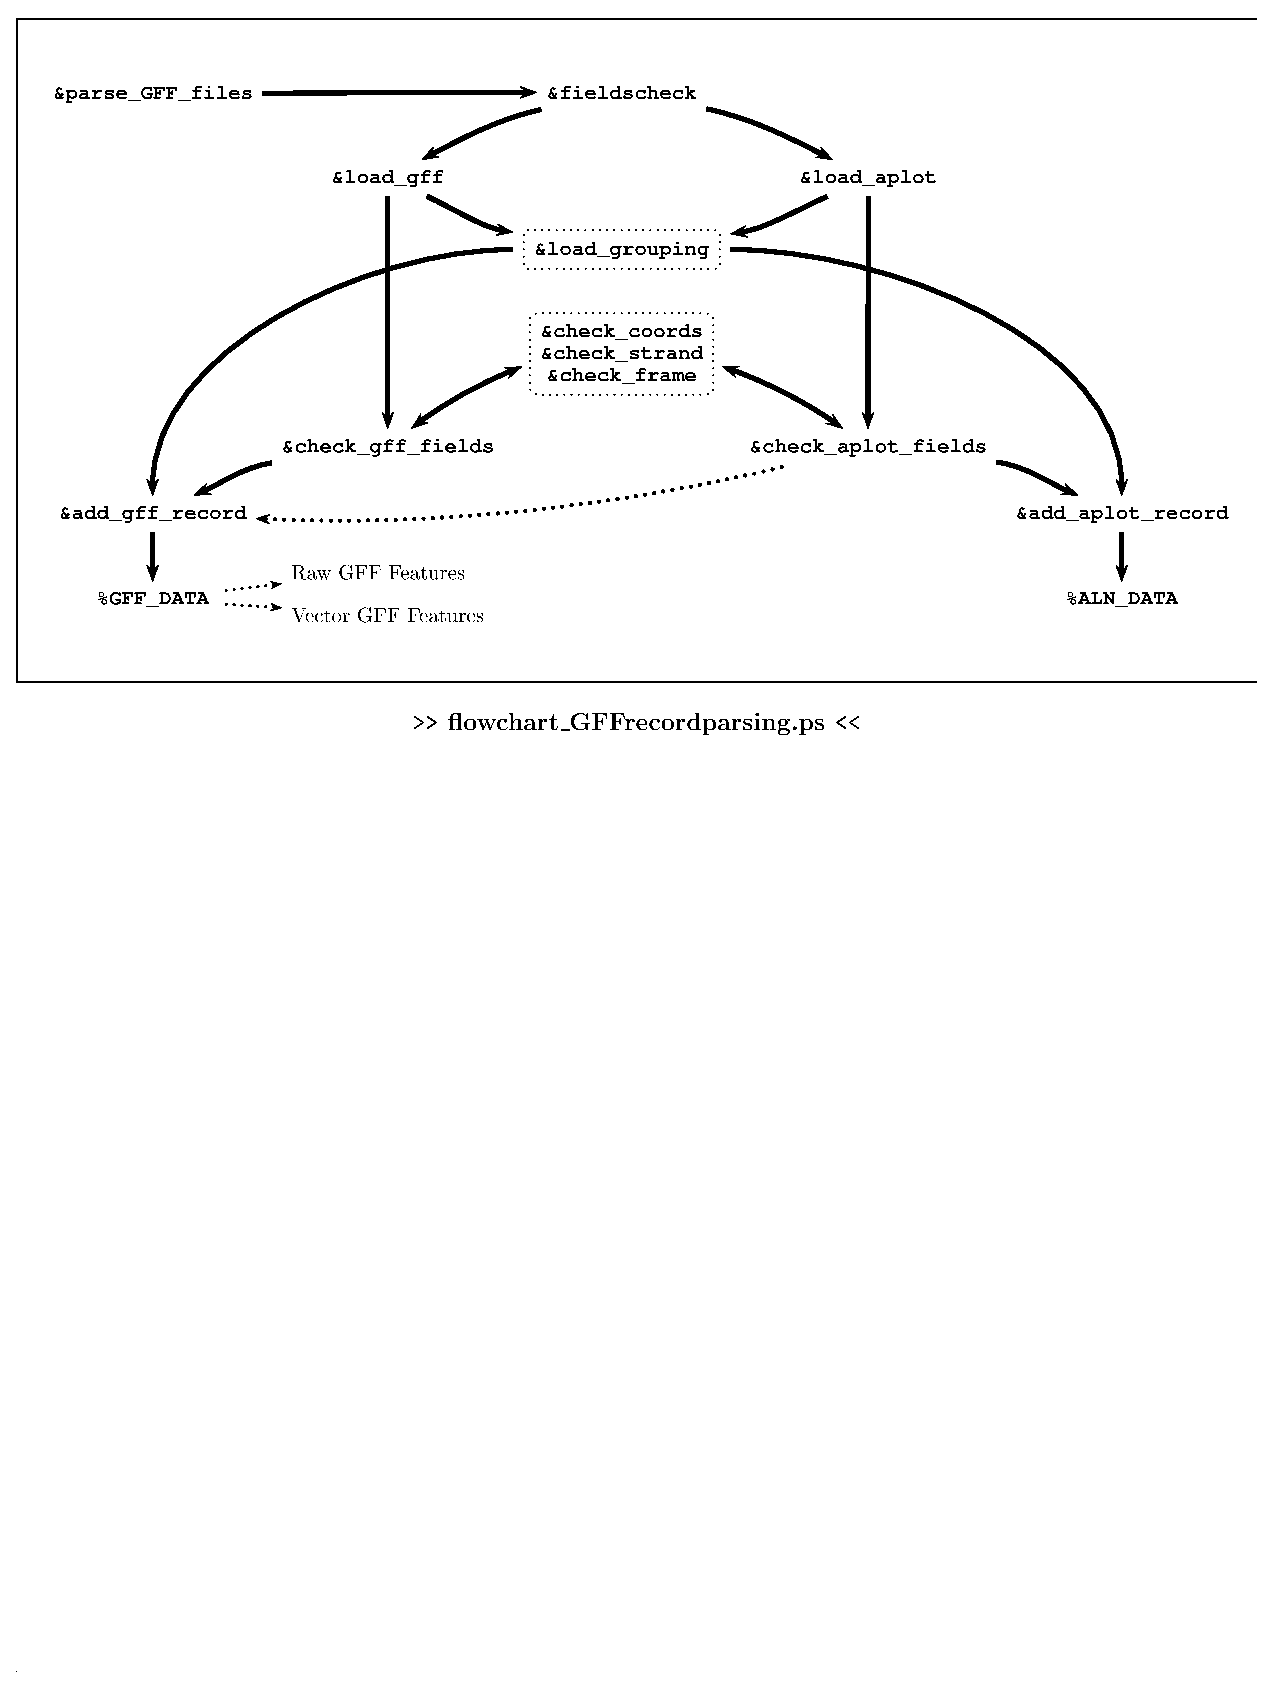
\includegraphics[bb=5 435 600 740,clip,width=\linewidth]
                 {./psfigures/flowchart_GFFrecordparsing.ps}
}%fbox
\caption[Flow diagram of the input GFF-records parsing.]{\label{fig:parsingGFF} Flow diagram of the input GFF-records parsing showing the main function names involved in this process.}
\end{center}
\end{figure}

\nwenddocs{}%
%
%
%
%
%
%
%
%
%
%
%
%
%
%
%
%
%
%
%
%
%
%
%
%
%
%
%
%
%
%
%
%
%
%
%
%
%
%
%
%
%
\nwbegindocs{730}\nwdocspar
\begin{table}[!t]
% \newcommand{\m}[1]{\multicolumn{2}{@{}c@{}}{#1}}
\begin{center}
 \input tables/GFF_regexes.tex
\end{center}
\end{table}


Function '{\tt{}{\char38}parse{\char95}GFF{\char95}files}' is only a wrapper for reporting the parsing process over GFF records. The main function call is '{\tt{}\protect\nwindexuse{{\char38}fieldscheck}{:amfieldscheck}{NWgff18-ParI-3}{\char38}fieldscheck}',which processes each GFF record and loads the values in its fields to the corresponding data structure. Although that, the wrapper checks if there are enough fields (8 required at least) and removes also any comment from the input record, assuming that a white space or a tab followed by a '{\tt{}{\char35}}' (as shown in this regular expression: '{\tt{}\ /{\char92}s+{\char92}{\char35}/\ }') is a comment mark, from there to the end of line everything is ignored.

\nwenddocs{}\nwbegincode{731}\sublabel{NWgff18-ParI-1}\nwmargintag{{\nwtagstyle{}\subpageref{NWgff18-ParI-1}}}\moddef{Parsing Input Data~{\nwtagstyle{}\subpageref{NWgff18-ParI-1}}}\endmoddef
sub parse_GFF_files() \{
    &header("PARSING INPUT GFF RECORDS");
  LOAD: foreach $file (@data_files) \{
      open(THIS,"< $file") ||
          (&warn('FILE_NO_OPEN',$T,$file), next LOAD);
      $file eq '-' && ($file = 'STANDARD INPUT');
      &report('READ_GFF_FILE',$file);
      ($n,$c) = (0,undef);
      while (<THIS>) \{
          my (@line,$main);
          ($c = '.', next) if /^\\#/o;
          ($c = '.', next) if /^\\s*$/o;
          chomp;
          # $c = $noGFF;
          ($main,undef) = split /\\s+\\#/o;
          @line = split /\\s+/o, $main, 9;        
          scalar(@line) < 8 &&
              (&warn('NOT_ENOUGH_FIELDS',$F,$file,$n,join(" ",@line)), next);
          $c = &GFF_format(&fieldscheck(\\@line));
      \} continue \{
          &counter(++$n,$c);
      \}; # WHILE
      &counter_end($n,$c);
      close(THIS);
  \}; # LOAD
    print LOGFILE (Data::Dumper->Dump([ \\%GFF_DATA, \\%ALN_DATA  ],
                                   [ qw( *GFF_DATA   *ALN_DATA ) ]))
        if ($LogFile && $Debug);
    &footer("DATA LOADED");
\} # sub parse_GFF
\nwindexdefn{{\char38}parse{\char95}GFF}{:amparse:unGFF}{NWgff18-ParI-1}\eatline
\nwidentdefs{\\{{{\char38}parse{\char95}GFF}{:amparse:unGFF}}}\nwidentuses{\\{{{\char38}GFF{\char95}format}{:amGFF:unformat}}\\{{{\char38}fieldscheck}{:amfieldscheck}}\\{{{\char38}footer}{:amfooter}}\\{{{\char38}header}{:amheader}}\\{{{\char38}report}{:amreport}}\\{{{\char38}warn}{:amwarn}}}\nwindexuse{{\char38}GFF{\char95}format}{:amGFF:unformat}{NWgff18-ParI-1}\nwindexuse{{\char38}fieldscheck}{:amfieldscheck}{NWgff18-ParI-1}\nwindexuse{{\char38}footer}{:amfooter}{NWgff18-ParI-1}\nwindexuse{{\char38}header}{:amheader}{NWgff18-ParI-1}\nwindexuse{{\char38}report}{:amreport}{NWgff18-ParI-1}\nwindexuse{{\char38}warn}{:amwarn}{NWgff18-ParI-1}\nwalsodefined{\\{NWgff18-ParI-2}\\{NWgff18-ParI-3}\\{NWgff18-ParI-4}\\{NWgff18-ParI-5}\\{NWgff18-ParI-6}\\{NWgff18-ParI-7}\\{NWgff18-ParI-8}\\{NWgff18-ParI-9}\\{NWgff18-ParI-A}\\{NWgff18-ParI-B}\\{NWgff18-ParI-C}\\{NWgff18-ParI-D}\\{NWgff18-ParI-E}\\{NWgff18-ParI-F}\\{NWgff18-ParI-G}\\{NWgff18-ParI-H}\\{NWgff18-ParI-I}\\{NWgff18-ParI-J}\\{NWgff18-ParI-K}}\nwused{\\{NWgff18-MaiD-1}}\nwendcode{}\nwbegindocs{732}%$ print LOGFILE '>>> \%GFF_DATA : '.(Dumper(\%GFF_DATA))


We define the following constants, used to report which format was found in the current read record (See table~\ref{tbl:DTkeysXreport}).

\nwenddocs{}%
%
%
%
%
%
%
%
%
%
%
%
%
%
%
%
%
%
%
%
%
%
\nwbegindocs{734}\nwdocspar
\begin{table}[!t]
\begin{center}
 \input tables/GFF_parser_codes.tex
\end{center}
\end{table}

\nwenddocs{}\nwbegincode{735}\sublabel{NWgff18-PreH-8}\nwmargintag{{\nwtagstyle{}\subpageref{NWgff18-PreH-8}}}\moddef{Pre-Declared Vars~{\nwtagstyle{}\subpageref{NWgff18-PreH-1}}}\plusendmoddef
$GFF $GFF_NOGP $VECTOR $ALIGN $APLOT $APLOT_NOGP $noGFF
\nwendcode{}\nwbegindocs{736}\nwdocspar
\nwenddocs{}\nwbegincode{737}\sublabel{NWgff18-GloG-8}\nwmargintag{{\nwtagstyle{}\subpageref{NWgff18-GloG-8}}}\moddef{Global Constants~{\nwtagstyle{}\subpageref{NWgff18-GloG-1}}}\plusendmoddef
($GFF,$GFF_NOGP,$VECTOR,$ALIGN,
    $APLOT,$APLOT_NOGP,$noGFF) =
    qw/ X x V A O o ? /;
\nwendcode{}\nwbegindocs{738}\nwdocspar

\nwenddocs{}\nwbegincode{739}\sublabel{NWgff18-warS-1}\nwmargintag{{\nwtagstyle{}\subpageref{NWgff18-warS-1}}}\moddef{warnings - parsing GFF files~{\nwtagstyle{}\subpageref{NWgff18-warS-1}}}\endmoddef
NOT_ENOUGH_FIELDS =>
  $Warn."Not enough fields in file \\"\\%s\\", line \\%s :\\n\\t\\%s\\n",
\nwidentuses{\\{{line}{line}}}\nwindexuse{line}{line}{NWgff18-warS-1}\nwalsodefined{\\{NWgff18-warS-2}\\{NWgff18-warS-3}\\{NWgff18-warS-4}\\{NWgff18-warS-5}}\nwused{\\{NWgff18-GloB-M}}\nwendcode{}\nwbegindocs{740}\nwdocspar

\nwenddocs{}\nwbegincode{741}\sublabel{NWgff18-mesS-1}\nwmargintag{{\nwtagstyle{}\subpageref{NWgff18-mesS-1}}}\moddef{messages - parsing GFF files~{\nwtagstyle{}\subpageref{NWgff18-mesS-1}}}\endmoddef
READ_GFF_FILE => 
  $sp."### Reading GFF records from \\"\\%s\\"\\n".$sp,
\nwused{\\{NWgff18-GloB-M}}\nwendcode{}\nwbegindocs{742}\nwdocspar

We set the character being printed in the parsing status output.

\nwenddocs{}\nwbegincode{743}\sublabel{NWgff18-ParI-2}\nwmargintag{{\nwtagstyle{}\subpageref{NWgff18-ParI-2}}}\moddef{Parsing Input Data~{\nwtagstyle{}\subpageref{NWgff18-ParI-1}}}\plusendmoddef
sub GFF_format() \{
    my $gff = $_[0];
    # return "x" if $GFF == $version1;
    return $GFF        if $gff eq $GFF;        # $version2
    return $GFF_NOGP   if $gff eq $GFF_NOGP;   # $version2 (ungrouped)
    return $VECTOR     if $gff eq $VECTOR;     # VECTOR: GFFv2 particular case 
    return $ALIGN      if $gff eq $ALIGN;      # ALIGN: GFFv2 particular case
    return $APLOT      if $gff eq $APLOT;      # Old aplot format (with colons)
    return $APLOT_NOGP if $gff eq $APLOT_NOGP; # Old aplot format (ungrouped)
    return $noGFF;
\} # GFF_format
\nwindexdefn{{\char38}GFF{\char95}format}{:amGFF:unformat}{NWgff18-ParI-2}\eatline
\nwidentdefs{\\{{{\char38}GFF{\char95}format}{:amGFF:unformat}}}\nwendcode{}\nwbegindocs{744}%$

Here we decide to parse records as they are in GFF or in APLOT format. '{\tt{}load{\char95}gff}' and '{\tt{}load{\char95}aplot}' do the field error checking and load the program variables '{\tt{}{\char37}GFF{\char95}DATA}' and '{\tt{}{\char37}ALN{\char95}DATA}'. Those variables are reset in '{\tt{}\LA{}Main Loop~{\nwtagstyle{}\subpageref{NWgff18-Mai9-1}}\RA{}}'.

\nwenddocs{}\nwbegincode{745}\sublabel{NWgff18-ParI-3}\nwmargintag{{\nwtagstyle{}\subpageref{NWgff18-ParI-3}}}\moddef{Parsing Input Data~{\nwtagstyle{}\subpageref{NWgff18-ParI-1}}}\plusendmoddef
sub fieldscheck() \{
    my ($list) = @_;
    my ($seqname,$start,$end) = @$list[0,3,4]; 
                              # ($list->[0],$list->[3],$list->[4]);
    (&fcolon($seqname) && &fcolon($start) && &fcolon($end)) && do \{
        return &load_aplot($list);
    \};
    return &load_gff($list);
\} # fieldscheck
\nwindexdefn{{\char38}fieldscheck}{:amfieldscheck}{NWgff18-ParI-3}\eatline
\nwidentdefs{\\{{{\char38}fieldscheck}{:amfieldscheck}}}\nwidentuses{\\{{{\char38}fcolon}{:amfcolon}}\\{{{\char38}load{\char95}aplot}{:amload:unaplot}}\\{{{\char38}load{\char95}gff}{:amload:ungff}}}\nwindexuse{{\char38}fcolon}{:amfcolon}{NWgff18-ParI-3}\nwindexuse{{\char38}load{\char95}aplot}{:amload:unaplot}{NWgff18-ParI-3}\nwindexuse{{\char38}load{\char95}gff}{:amload:ungff}{NWgff18-ParI-3}\nwendcode{}\nwbegindocs{746}\nwdocspar
For historical reasons the program can work with APLOT format (see Table~\ref{tbl:formats}). Initial field checking determines whether the record being processed is under that alignment GFF-like format, by determining that first, fourth and fifth fields contain a colon char. Then we assume we are under APLOT format.

\nwenddocs{}\nwbegincode{747}\sublabel{NWgff18-ParI-4}\nwmargintag{{\nwtagstyle{}\subpageref{NWgff18-ParI-4}}}\moddef{Parsing Input Data~{\nwtagstyle{}\subpageref{NWgff18-ParI-1}}}\plusendmoddef
sub fcolon() \{ return ($_[0] =~ /^.+:.+$/o ? $T : $F) \}
\nwindexdefn{{\char38}fcolon}{:amfcolon}{NWgff18-ParI-4}\eatline
\nwidentdefs{\\{{{\char38}fcolon}{:amfcolon}}}\nwendcode{}\nwbegindocs{748}\nwdocspar
\subsctn{Validating fields}

The following functions checks whether some of the input GFF fields are well defined. They return '{\tt{}True}' ('{\tt{}{\char36}T}') if no error found and '{\tt{}False}' ('{\tt{}{\char36}F}') when input fields are wrong. The returned value forces '{\tt{}\protect\nwindexuse{{\char38}load{\char95}aplot}{:amload:unaplot}{NWgff18-ParI-B}{\char38}load{\char95}aplot}' or '{\tt{}\protect\nwindexuse{{\char38}load{\char95}gff}{:amload:ungff}{NWgff18-ParI-9}{\char38}load{\char95}gff}' functions to skip the records having format errors.

Here we test that '\pa{start}' field must be lower or equal than '\pa{end}' in standard GFF-records. From now on, it is also required for the second coords pair if we get coords from aplot records.

\label{func:checkcoords}
\nwenddocs{}\nwbegincode{749}\sublabel{NWgff18-ParI-5}\nwmargintag{{\nwtagstyle{}\subpageref{NWgff18-ParI-5}}}\moddef{Parsing Input Data~{\nwtagstyle{}\subpageref{NWgff18-ParI-1}}}\plusendmoddef
sub check_coords() \{ # ((ori,end)_1,...,(ori,end)_n)
    my ($aflg,@ary) = @_;
    for (my $j=0; $j<=$#ary; $j+=2) \{
        $ary[$j] > $ary[$j+1] && do \{
            &warn('ORI_GREATER_END',$F,$ary[$j],$ary[$j+1],$file,$n+1);
            return $F;
        \}; # $ary[$j] > $ary[$j+1]
    \}; # for
    return $T;
\} # check_coords
\nwindexdefn{{\char38}check{\char95}coords}{:amcheck:uncoords}{NWgff18-ParI-5}\eatline
\nwidentdefs{\\{{{\char38}check{\char95}coords}{:amcheck:uncoords}}}\nwidentuses{\\{{{\char38}warn}{:amwarn}}}\nwindexuse{{\char38}warn}{:amwarn}{NWgff18-ParI-5}\nwendcode{}\nwbegindocs{750}\nwdocspar
\nwenddocs{}\nwbegincode{751}\sublabel{NWgff18-warS-2}\nwmargintag{{\nwtagstyle{}\subpageref{NWgff18-warS-2}}}\moddef{warnings - parsing GFF files~{\nwtagstyle{}\subpageref{NWgff18-warS-1}}}\plusendmoddef
ORI_GREATER_END =>
  $Warn."Start greater than end \\"\\%s > \\%s\\" in file \\"\\%s\\" line \\"\\%s\\".\\n", 
\nwidentuses{\\{{line}{line}}}\nwindexuse{line}{line}{NWgff18-warS-2}\nwendcode{}\nwbegindocs{752}\nwdocspar

'\pa{score}' field may contain '.' (for records having no score), we change score for those cases to '0'.

\nwenddocs{}\nwbegincode{753}\sublabel{NWgff18-ParI-6}\nwmargintag{{\nwtagstyle{}\subpageref{NWgff18-ParI-6}}}\moddef{Parsing Input Data~{\nwtagstyle{}\subpageref{NWgff18-ParI-1}}}\plusendmoddef
sub check_score() \{ # (scoref_1,...,scoref_n)
    foreach my $sco (@_) \{
        (defined($$sco) && $$sco eq '.') && ($$sco = 0);
    \}; # foreach
\} # check_score
\nwindexdefn{{\char38}check{\char95}score}{:amcheck:unscore}{NWgff18-ParI-6}\eatline
\nwidentdefs{\\{{{\char38}check{\char95}score}{:amcheck:unscore}}}\nwendcode{}\nwbegindocs{754}\nwdocspar
'\pa{strand}' field must contain only '+', '-' or '.' (for records having no strand).

\nwenddocs{}\nwbegincode{755}\sublabel{NWgff18-ParI-7}\nwmargintag{{\nwtagstyle{}\subpageref{NWgff18-ParI-7}}}\moddef{Parsing Input Data~{\nwtagstyle{}\subpageref{NWgff18-ParI-1}}}\plusendmoddef
sub check_strand() \{ # (str_1,...,srt_n)
    foreach my $str (@_) \{
        $str !~ /$regexp_strand/o && do \{
            &warn('STRAND_MISMATCH',$F,$str,$file,$n+1);
            return $F;
        \};
    \}; # foreach
    return $T;
\} # check_strand
\nwindexdefn{{\char38}check{\char95}strand}{:amcheck:unstrand}{NWgff18-ParI-7}\eatline
\nwidentdefs{\\{{{\char38}check{\char95}strand}{:amcheck:unstrand}}}\nwidentuses{\\{{{\char36}regexp{\char95}strand}{:doregexp:unstrand}}\\{{{\char38}warn}{:amwarn}}}\nwindexuse{{\char36}regexp{\char95}strand}{:doregexp:unstrand}{NWgff18-ParI-7}\nwindexuse{{\char38}warn}{:amwarn}{NWgff18-ParI-7}\nwendcode{}\nwbegindocs{756}\nwdocspar
\nwenddocs{}\nwbegincode{757}\sublabel{NWgff18-warS-3}\nwmargintag{{\nwtagstyle{}\subpageref{NWgff18-warS-3}}}\moddef{warnings - parsing GFF files~{\nwtagstyle{}\subpageref{NWgff18-warS-1}}}\plusendmoddef
STRAND_MISMATCH =>
  $Warn." Strand mismatch definition \\"\\%s\\" in file \\"\\%s\\" line \\"\\%s\\".\\n",
\nwidentuses{\\{{line}{line}}}\nwindexuse{line}{line}{NWgff18-warS-3}\nwendcode{}\nwbegindocs{758}\nwdocspar

Same happens to '\pa{frame}', which only '0', '1', '2' or '.' (for those records having no frame) values are allowed.

\nwenddocs{}\nwbegincode{759}\sublabel{NWgff18-ParI-8}\nwmargintag{{\nwtagstyle{}\subpageref{NWgff18-ParI-8}}}\moddef{Parsing Input Data~{\nwtagstyle{}\subpageref{NWgff18-ParI-1}}}\plusendmoddef
sub check_frame() \{ # (frm_1,...,frm_n)
    foreach my $frm (@_) \{
        $frm !~ /$regexp_frame/o && do \{
            &warn('FRAME_MISMATCH',$F,$frm,$file,$n+1);
            return $F;
        \};
    \}; # foreach
    return $T;
\} # check_frame
\nwindexdefn{{\char38}check{\char95}frame}{:amcheck:unframe}{NWgff18-ParI-8}\eatline
\nwidentdefs{\\{{{\char38}check{\char95}frame}{:amcheck:unframe}}}\nwidentuses{\\{{{\char36}regexp{\char95}frame}{:doregexp:unframe}}\\{{{\char38}warn}{:amwarn}}}\nwindexuse{{\char36}regexp{\char95}frame}{:doregexp:unframe}{NWgff18-ParI-8}\nwindexuse{{\char38}warn}{:amwarn}{NWgff18-ParI-8}\nwendcode{}\nwbegindocs{760}\nwdocspar
\nwenddocs{}\nwbegincode{761}\sublabel{NWgff18-PreP-2}\nwmargintag{{\nwtagstyle{}\subpageref{NWgff18-PreP-2}}}\moddef{Pre-Declared Vars: regexp~{\nwtagstyle{}\subpageref{NWgff18-PreP-1}}}\plusendmoddef
$regexp_frame
\nwindexdefn{{\char36}regexp{\char95}frame}{:doregexp:unframe}{NWgff18-PreP-2}\eatline
\nwidentdefs{\\{{{\char36}regexp{\char95}frame}{:doregexp:unframe}}}\nwendcode{}\nwbegincode{762}\sublabel{NWgff18-GloG-9}\nwmargintag{{\nwtagstyle{}\subpageref{NWgff18-GloG-9}}}\moddef{Global Constants~{\nwtagstyle{}\subpageref{NWgff18-GloG-1}}}\plusendmoddef
$regexp_frame = '^[.012]$'; #'
\nwidentuses{\\{{{\char36}regexp{\char95}frame}{:doregexp:unframe}}}\nwindexuse{{\char36}regexp{\char95}frame}{:doregexp:unframe}{NWgff18-GloG-9}\nwendcode{}\nwbegindocs{763}\nwdocspar

\nwenddocs{}\nwbegincode{764}\sublabel{NWgff18-warS-4}\nwmargintag{{\nwtagstyle{}\subpageref{NWgff18-warS-4}}}\moddef{warnings - parsing GFF files~{\nwtagstyle{}\subpageref{NWgff18-warS-1}}}\plusendmoddef
FRAME_MISMATCH =>
  $Warn." Frame mismatch definition \\"\\%s\\" in file \\"\\%s\\" line \\"\\%s\\".\\n",
\nwidentuses{\\{{line}{line}}}\nwindexuse{line}{line}{NWgff18-warS-4}\nwendcode{}\nwbegindocs{765}\nwdocspar


\subsubsctn{Checking for strands}

\nwenddocs{}\nwbegincode{766}\sublabel{NWgff18-varN-K}\nwmargintag{{\nwtagstyle{}\subpageref{NWgff18-varN-K}}}\moddef{variable value checking~{\nwtagstyle{}\subpageref{NWgff18-varN-1}}}\plusendmoddef
STRAND => sub \{ # Value, varName, Lowercase
      my ($_v,$_n,undef) = @_;
      $$_v =~ /$regexp_strand/o && return $T;
      &warn('NOT_A_STRAND',$F,$$_v,$_n);
      return $F;
  \},
\nwindexdefn{{\char123}STRAND{\char125}}{:lbSTRAND:rb}{NWgff18-varN-K}\eatline
\nwidentdefs{\\{{{\char123}STRAND{\char125}}{:lbSTRAND:rb}}}\nwidentuses{\\{{{\char36}regexp{\char95}strand}{:doregexp:unstrand}}\\{{{\char38}warn}{:amwarn}}}\nwindexuse{{\char36}regexp{\char95}strand}{:doregexp:unstrand}{NWgff18-varN-K}\nwindexuse{{\char38}warn}{:amwarn}{NWgff18-varN-K}\nwendcode{}\nwbegindocs{767}\nwdocspar
\nwenddocs{}\nwbegincode{768}\sublabel{NWgff18-PreP-3}\nwmargintag{{\nwtagstyle{}\subpageref{NWgff18-PreP-3}}}\moddef{Pre-Declared Vars: regexp~{\nwtagstyle{}\subpageref{NWgff18-PreP-1}}}\plusendmoddef
$regexp_strand
\nwindexdefn{{\char36}regexp{\char95}strand}{:doregexp:unstrand}{NWgff18-PreP-3}\eatline
\nwidentdefs{\\{{{\char36}regexp{\char95}strand}{:doregexp:unstrand}}}\nwendcode{}\nwbegincode{769}\sublabel{NWgff18-GloG-A}\nwmargintag{{\nwtagstyle{}\subpageref{NWgff18-GloG-A}}}\moddef{Global Constants~{\nwtagstyle{}\subpageref{NWgff18-GloG-1}}}\plusendmoddef
$regexp_strand = '^[+-.]$'; #'
\nwidentuses{\\{{{\char36}regexp{\char95}strand}{:doregexp:unstrand}}}\nwindexuse{{\char36}regexp{\char95}strand}{:doregexp:unstrand}{NWgff18-GloG-A}\nwendcode{}\nwbegindocs{770}\nwdocspar
     
\nwenddocs{}\nwbegincode{771}\sublabel{NWgff18-warS-5}\nwmargintag{{\nwtagstyle{}\subpageref{NWgff18-warS-5}}}\moddef{warnings - parsing GFF files~{\nwtagstyle{}\subpageref{NWgff18-warS-1}}}\plusendmoddef
NOT_A_STRAND =>
  $Warn."\\"\\%s\\" STRAND not recognized on \\"\\%s\\"... ".
  "Must be [+], [.] or [-]\\n",
\nwendcode{}\nwbegindocs{772}\nwdocspar


\subsctn{Parsing standard GFF format}
\label{sec:parseGFF}

'{\tt{}\protect\nwindexuse{{\char38}check{\char95}gff{\char95}fields}{:amcheck:ungff:unfields}{NWgff18-ParI-A}{\char38}check{\char95}gff{\char95}fields}' will call to the '{\tt{}\protect\nwindexuse{{\char38}add{\char95}gff{\char95}record}{:amadd:ungff:unrecord}{NWgff18-ParI-E}{\char38}add{\char95}gff{\char95}record}' which loads the new record if everything is OK into '{\tt{}{\char37}GFF{\char95}DATA}' (see section~\ref{sec:GFFhsh}, page~\pageref{sec:GFFhsh}). The first parameter for '{\tt{}\protect\nwindexuse{{\char38}load{\char95}grouping}{:amload:ungrouping}{NWgff18-ParI-I}{\char38}load{\char95}grouping}' function is set to 'True' for GFF grouping definition ('False' is for APLOT grouping definition, see section~\ref{sec:parseAPLOT}). 

\nwenddocs{}\nwbegincode{773}\sublabel{NWgff18-ParI-9}\nwmargintag{{\nwtagstyle{}\subpageref{NWgff18-ParI-9}}}\moddef{Parsing Input Data~{\nwtagstyle{}\subpageref{NWgff18-ParI-1}}}\plusendmoddef
sub load_gff() \{ # if errors found > return $noGFF
    my ($list) = @_ ;
    my $w_gff;
    ($seqname,$source,$feature,$start,$end,
     $score,$strand,$frame) = @$list[0,1,2,3,4,5,6,7];
    $w_gff = &load_grouping($T,$list->[8]);
    &check_gff_fields($w_gff) || ($w_gff=$noGFF);
    return $w_gff;
\} # load_gff
\nwindexdefn{{\char38}load{\char95}gff}{:amload:ungff}{NWgff18-ParI-9}\eatline
\nwidentdefs{\\{{{\char38}load{\char95}gff}{:amload:ungff}}}\nwidentuses{\\{{{\char38}check{\char95}gff{\char95}fields}{:amcheck:ungff:unfields}}\\{{{\char38}load{\char95}grouping}{:amload:ungrouping}}}\nwindexuse{{\char38}check{\char95}gff{\char95}fields}{:amcheck:ungff:unfields}{NWgff18-ParI-9}\nwindexuse{{\char38}load{\char95}grouping}{:amload:ungrouping}{NWgff18-ParI-9}\nwendcode{}\nwbegindocs{774}\nwdocspar
\nwenddocs{}\nwbegincode{775}\sublabel{NWgff18-GloB-F}\nwmargintag{{\nwtagstyle{}\subpageref{NWgff18-GloB-F}}}\moddef{Global Vars~{\nwtagstyle{}\subpageref{NWgff18-GloB-1}}}\plusendmoddef
my ($seqname,$source,$feature,$start,
    $end,$score,$strand,$frame); # GFF temporary vars
\nwendcode{}\nwbegindocs{776}\nwdocspar

\subsubsctn{Checking fields and accepting GFF records}

\nwenddocs{}\nwbegincode{777}\sublabel{NWgff18-ParI-A}\nwmargintag{{\nwtagstyle{}\subpageref{NWgff18-ParI-A}}}\moddef{Parsing Input Data~{\nwtagstyle{}\subpageref{NWgff18-ParI-1}}}\plusendmoddef
sub check_gff_fields() \{
    &check_coords($T,$start,$end) || (return $F);
    &check_strand($strand) || (return $F);
    &check_score(\\$score);
    &check_frame($frame) || (return $F);
    &add_gff_record($_[0]);
    return $T; 
\} # check_gff_fields
\nwindexdefn{{\char38}check{\char95}gff{\char95}fields}{:amcheck:ungff:unfields}{NWgff18-ParI-A}\eatline
\nwidentdefs{\\{{{\char38}check{\char95}gff{\char95}fields}{:amcheck:ungff:unfields}}}\nwidentuses{\\{{{\char38}add{\char95}gff{\char95}record}{:amadd:ungff:unrecord}}\\{{{\char38}check{\char95}coords}{:amcheck:uncoords}}\\{{{\char38}check{\char95}frame}{:amcheck:unframe}}\\{{{\char38}check{\char95}score}{:amcheck:unscore}}\\{{{\char38}check{\char95}strand}{:amcheck:unstrand}}}\nwindexuse{{\char38}add{\char95}gff{\char95}record}{:amadd:ungff:unrecord}{NWgff18-ParI-A}\nwindexuse{{\char38}check{\char95}coords}{:amcheck:uncoords}{NWgff18-ParI-A}\nwindexuse{{\char38}check{\char95}frame}{:amcheck:unframe}{NWgff18-ParI-A}\nwindexuse{{\char38}check{\char95}score}{:amcheck:unscore}{NWgff18-ParI-A}\nwindexuse{{\char38}check{\char95}strand}{:amcheck:unstrand}{NWgff18-ParI-A}\nwendcode{}\nwbegindocs{778}\nwdocspar
\begin{table}[!t]
\begin{center}
\input tables/DataStructure_GFF.tex
\caption[GFF internal data structure for {\prog}]{\label{tbl:gffdata} GFF internal data structure for {\prog}. The topmost hash corresponds to '{\tt{}{\char37}GFF{\char95}DATA}', the others are anonymous lists/hashes expanding from it.}
\end{center}
\end{table}

%%%%%%%%%%%%%%%%%%%%%%%%%%%%%%%%%%%%%%%%%%%%%%%%%%%%%%%%%%%%%%%%%
\nwenddocs{}%
%
%
%
%
%
%
%
%
%
%
%
%
%
%
%
%
%
%
%
%
%
%
%
%
%
%
%
%
%
%
%
%
%
%
%
%
%
%
%
%
%
%
%
%
%
%
%
%
%
%
%
%
%
%
%
%
%
%
%
%
%
%
%
%
%
%
%
%
%
\nwbegindocs{780}\nwdocspar
%%%%%%%%%%%%%%%%%%%%%%%%%%%%%%%%%%%%%%%%%%%%%%%%%%%%%%%%%%%%%%%%%%%


\subsctn{Parsing APLOT format}
\label{sec:parseAPLOT}

'{\tt{}\protect\nwindexuse{{\char38}check{\char95}aplot{\char95}fields}{:amcheck:unaplot:unfields}{NWgff18-ParI-D}{\char38}check{\char95}aplot{\char95}fields}' will call to the '{\tt{}{\char38}add{\char95}aplot{\char95}record}' which loads the new record if everything is OK into '{\tt{}{\char37}ALN{\char95}DATA}' (see section~\ref{sec:APLOThsh}, page~\pageref{sec:APLOThsh}). The first parameter for '{\tt{}\protect\nwindexuse{{\char38}load{\char95}grouping}{:amload:ungrouping}{NWgff18-ParI-I}{\char38}load{\char95}grouping}' function is set to 'False' is for APLOT grouping definition ('True' for GFF grouping definition, see section~\ref{sec:parseGFF}). To optimize feature search later, now {\tt{}\protect\nwindexuse{{\char38}remove{\char95}colon}{:amremove:uncolon}{NWgff18-ParI-C}{\char38}remove{\char95}colon} can return undefined values; so that, we have to check if {\tt{}{\char36}strand{\char95}2} and {\tt{}{\char36}frame{\char95}2} are defined or not, to set the corresponding equivalence, but we do not do the same for {\tt{}{\char36}source{\char95}2} and {\tt{}{\char36}feature{\char95}2} (see {\tt{}\LA{}select GFF or ALN settings~{\nwtagstyle{}\subpageref{NWgff18-selQ-1}}\RA{}} code chunk to see what we do now when these last two vars were not defined).

\nwenddocs{}\nwbegincode{781}\sublabel{NWgff18-ParI-B}\nwmargintag{{\nwtagstyle{}\subpageref{NWgff18-ParI-B}}}\moddef{Parsing Input Data~{\nwtagstyle{}\subpageref{NWgff18-ParI-1}}}\plusendmoddef
sub load_aplot() \{ # if errors found > return $noGFF
    my ($list) = @_;
    my $w_gff;
    ($seqname_1,$seqname_2,$source_1,$source_2,$feature_1,$feature_2,
     $start_1,$start_2,$end_1,$end_2,
     $strand_1,$strand_2,$frame_1,$frame_2) = 
     &remove_colon(@$list[0,1,2,3,4,6,7]);
    defined($strand_2) || ($strand_2 = $strand_1);
    defined($frame_2)  || ($frame_2  = $frame_1 );
    ($score_1,$score_2) = ($list->[5], undef);
    $w_gff = &load_grouping($F,$list->[8]);
    &check_aplot_fields($w_gff) || ($w_gff=$noGFF);
    return $w_gff;
\} # load_aplot
\nwindexdefn{{\char38}load{\char95}aplot}{:amload:unaplot}{NWgff18-ParI-B}\eatline
\nwidentdefs{\\{{{\char38}load{\char95}aplot}{:amload:unaplot}}}\nwidentuses{\\{{{\char38}check{\char95}aplot{\char95}fields}{:amcheck:unaplot:unfields}}\\{{{\char38}load{\char95}grouping}{:amload:ungrouping}}\\{{{\char38}remove{\char95}colon}{:amremove:uncolon}}}\nwindexuse{{\char38}check{\char95}aplot{\char95}fields}{:amcheck:unaplot:unfields}{NWgff18-ParI-B}\nwindexuse{{\char38}load{\char95}grouping}{:amload:ungrouping}{NWgff18-ParI-B}\nwindexuse{{\char38}remove{\char95}colon}{:amremove:uncolon}{NWgff18-ParI-B}\nwendcode{}\nwbegindocs{782}%$

We reserve {\tt{}{\char36}score{\char95}2} for other scores than can be passed, we may have bit-scores in '{\tt{}score}' field (so {\tt{}{\char36}score{\char95}1} will be set to that) and alignment-scores in a tag-value pair found in extra data from grouping fields (we will use them to set {\tt{}{\char36}score{\char95}2}), or viceversa. Although that could happen, we initialize {\tt{}{\char36}score{\char95}2} to an undefined value.

\nwenddocs{}\nwbegincode{783}\sublabel{NWgff18-GloB-G}\nwmargintag{{\nwtagstyle{}\subpageref{NWgff18-GloB-G}}}\moddef{Global Vars~{\nwtagstyle{}\subpageref{NWgff18-GloB-1}}}\plusendmoddef
my ($seqname_1,$seqname_2,
    $source_1,$source_2,$feature_1,$feature_2,
    $start_1,$start_2,$end_1,$end_2,$score_1,$score_2,
    $strand_1,$strand_2,$frame_1,$frame_2); # APLOT temporary vars
my ($tag,$group,$group_id,$label,
    $group_gff_counter,$group_aplot_counter); # GROUPING temporary vars
\nwendcode{}\nwbegindocs{784}\nwdocspar

\nwenddocs{}%
%
%
%
%
%
%
%
%
%
%
%
%
%
%
%
%
%
%
%
%
%
%
%
%
%
%
%
%
%
%
%
%
\nwbegindocs{786}\nwdocspar
\begin{table}[!t]
\begin{center}
 \input tables/missing_strands_substitution.tex
\end{center}
\end{table}

When checking for colons, we assume that any element defined without colons is equal to the same value repeated twice (see Table~\ref{tbl:missingfields}). 

\nwenddocs{}\nwbegincode{787}\sublabel{NWgff18-ParI-C}\nwmargintag{{\nwtagstyle{}\subpageref{NWgff18-ParI-C}}}\moddef{Parsing Input Data~{\nwtagstyle{}\subpageref{NWgff18-ParI-1}}}\plusendmoddef
sub remove_colon() \{
    my @ary_out = ();
    my ($a,$b) = (undef,undef);
    foreach my $fld (@_) \{
        ($a,$b) = split /:/o, $fld, 2;
        push @ary_out, (
            (defined($a) ? $a : '.'  ),
            (defined($b) ? $b : undef)
            );
    \};
    return @ary_out;
\} # remove_colon
\nwindexdefn{{\char38}remove{\char95}colon}{:amremove:uncolon}{NWgff18-ParI-C}\eatline
\nwidentdefs{\\{{{\char38}remove{\char95}colon}{:amremove:uncolon}}}\nwendcode{}\nwbegindocs{788}%$

\subsubsctn{Checking fields and accepting APLOT records}

If records are OK, then we can append a new record to the variable defined for APLOT records (so called as '{\tt{}{\char37}ALN{\char95}DATA}' in table~\ref{tbl:alndata}, page~\pageref{tbl:alndata}). \label{sec:APLOThsh}

\nwenddocs{}\nwbegincode{789}\sublabel{NWgff18-ParI-D}\nwmargintag{{\nwtagstyle{}\subpageref{NWgff18-ParI-D}}}\moddef{Parsing Input Data~{\nwtagstyle{}\subpageref{NWgff18-ParI-1}}}\plusendmoddef
sub check_aplot_fields() \{
    &check_coords($F,$start_1,$end_1,$start_2,$end_2) || (return $F);
    &check_strand($strand_1,$strand_2) || (return $F);
    &check_score(\\$score_1,\\$score_2);
    &check_frame($frame_1,$frame_2) || (return $F);
    &add_gff_record($_[0]);
    return $T; 
\} # check_aplot_fields
\nwindexdefn{{\char38}check{\char95}aplot{\char95}fields}{:amcheck:unaplot:unfields}{NWgff18-ParI-D}\eatline
\nwidentdefs{\\{{{\char38}check{\char95}aplot{\char95}fields}{:amcheck:unaplot:unfields}}}\nwidentuses{\\{{{\char38}add{\char95}gff{\char95}record}{:amadd:ungff:unrecord}}\\{{{\char38}check{\char95}coords}{:amcheck:uncoords}}\\{{{\char38}check{\char95}frame}{:amcheck:unframe}}\\{{{\char38}check{\char95}score}{:amcheck:unscore}}\\{{{\char38}check{\char95}strand}{:amcheck:unstrand}}}\nwindexuse{{\char38}add{\char95}gff{\char95}record}{:amadd:ungff:unrecord}{NWgff18-ParI-D}\nwindexuse{{\char38}check{\char95}coords}{:amcheck:uncoords}{NWgff18-ParI-D}\nwindexuse{{\char38}check{\char95}frame}{:amcheck:unframe}{NWgff18-ParI-D}\nwindexuse{{\char38}check{\char95}score}{:amcheck:unscore}{NWgff18-ParI-D}\nwindexuse{{\char38}check{\char95}strand}{:amcheck:unstrand}{NWgff18-ParI-D}\nwendcode{}\nwbegindocs{790}\nwdocspar
\begin{table}[!t]
\begin{center}
% \input tables/DataStructure_ALN.tex
\caption[Internal data structure to store alignments]{\label{tbl:alndata} Alignment data structure, so called '{\tt{}{\char37}ALN{\char95}DATA}', has same structure as '{\tt{}{\char37}GFF{\char95}DATA}' shown in table~\ref{tbl:gffdata}. Here we only show the small differences between them.}
\end{center}
\end{table}

\label{todo:ELA}
\nwenddocs{}%
%
%
%
%
\nwbegindocs{792}\nwdocspar
\nwenddocs{}%
%
\nwbegindocs{794}\nwdocspar
\todo{ \item \todoELA } % todo

%%%%%%%%%%%%%%%%%%%%%%%%%%%%%%%%%%%%%%%%%%%%%%%%%%%%%%%%%%%%%%%%%
\nwenddocs{}%
%
\nwbegindocs{796}\nwdocspar
%%%%%%%%%%%%%%%%%%%%%%%%%%%%%%%%%%%%%%%%%%%%%%%%%%%%%%%%%%%%%%%%%%%


\subsctn{Loading records to GFF/ALN hashes}

\nwenddocs{}%
%
\nwbegindocs{798}\nwdocspar

Once fields checking is done, we proceed to load the data structure defined for the GFF records or for the ALIGNMENT ones, we have merged the loading functions for both record types in the current version because they shared many common structures. 

In the first case we have to add the new record into '{\tt{}{\char37}GFF{\char95}DATA}' hash, the outline of the inner structure of that variable is shown in table~\ref{tbl:gffdata}, page~\pageref{tbl:gffdata}. \label{sec:GFFhsh}
On the other hand, ALIGMENT records need a pre-processing of some of the fields before being ready to fill '{\tt{}{\char37}ALN{\char95}DATA}' hash, table~\ref{tbl:alndata} in page~\pageref{tbl:alndata} summarizes the differences between this record type and the GFF one. \label{sec:ALNhsh}

\nwenddocs{}\nwbegincode{799}\sublabel{NWgff18-ParI-E}\nwmargintag{{\nwtagstyle{}\subpageref{NWgff18-ParI-E}}}\moddef{Parsing Input Data~{\nwtagstyle{}\subpageref{NWgff18-ParI-1}}}\plusendmoddef
sub add_gff_record() \{
    my $_gff = $_[0];
    my ($VarName,$Counter,$Type,$isaln,$myfunc,$t);
    \LA{}select GFF or ALN settings~{\nwtagstyle{}\subpageref{NWgff18-selQ-1}}\RA{}
    &load_var($seqname,$VarName,$Counter,$Type,$myfunc);
    ($VarName,$Counter,$Type) = (
        \\%\{$VarName->\{$seqname\}[$_element]\},
        \\$$VarName\{$seqname\}[$_counter][$_elemNum],
        'SOURCE' );
    &load_var($source,$VarName,$Counter,$Type,$myfunc);
    ($VarName,$Counter,$Type) = ( 
        \\%\{$VarName->\{$source\}[$_element]\},
        \\$$VarName\{$source\}[$_counter][$_elemNum],
        'STRAND' );
    &load_var($strand,$VarName,$Counter,$Type,$myfunc);
    ($VarName,$Counter,$Type) = (
        \\%\{$VarName->\{$strand\}[$_element]\},
        \\$$VarName\{$strand\}[$_counter][$_elemNum],
        'GROUP' );
    &load_var($group,$VarName,$Counter,$Type,$myfunc);
    \LA{}adding new feature elements~{\nwtagstyle{}\subpageref{NWgff18-addR-1}}\RA{}
    return;
\} # add_gff_record
\nosublabel{NWgff18-ParI-E-u2}\nwindexdefn{{\char38}add{\char95}gff{\char95}record}{:amadd:ungff:unrecord}{NWgff18-ParI-E}\eatline
\nwidentdefs{\\{{{\char38}add{\char95}gff{\char95}record}{:amadd:ungff:unrecord}}}\nwidentuses{\\{{{\char38}load{\char95}var}{:amload:unvar}}}\nwindexuse{{\char38}load{\char95}var}{:amload:unvar}{NWgff18-ParI-E}\nwendcode{}\nwbegindocs{800}\nwdocspar
If the standard GFF alignment format is found, we process those records as if they were aplot records, so that we have to set all the variables required to fill such data structure. We solve that by setting the same variables when loading those standard GFF alignment records as we do when loading aplot records, then they can share the same processes that are switched on by {\tt{}{\char36}isaln}.
% ('{\tt{}{\char38}add{\char95}aplot{\char95}record}' is described in section~\ref{func:loadalnvar}, page~\pageref{func:loadalnvar})

\nwenddocs{}\nwbegincode{801}\sublabel{NWgff18-selQ-1}\nwmargintag{{\nwtagstyle{}\subpageref{NWgff18-selQ-1}}}\moddef{select GFF or ALN settings~{\nwtagstyle{}\subpageref{NWgff18-selQ-1}}}\endmoddef
$isaln = ($_gff =~ /$ALIGN|$APLOT|$APLOT_NOGP/o) ? $T : $F;
ISALN: \{
    $isaln && do \{
        $myfunc = \\&load_aln_var;
        ($VarName,$Counter,$Type) = (
            \\%ALN_DATA,
            \\$aln_COUNT,
            'SEQUENCE' );
        $seqname = join(":", $seqname_1, $seqname_2);
        $source  = defined($source_2)
                   ? join(":", $source_1, $source_2)
                   : $source_1;
        $strand  = defined($strand_2) 
                   ? $strand_1.$strand_2
                   : $strand_1;
        $feature = defined($feature_2) 
                   ? join(":", $feature_1, $feature_2)
                   : $feature_1;
        last ISALN;
    \}; # $isaln
    $myfunc = \\&load_gff_var;
    ($VarName,$Counter,$Type) = (
        \\%GFF_DATA,
        \\$seq_COUNT,
        'SEQUENCE' );
\}; # ISALN
\nwidentuses{\\{{{\char38}load{\char95}aln{\char95}var}{:amload:unaln:unvar}}\\{{{\char38}load{\char95}gff{\char95}var}{:amload:ungff:unvar}}}\nwindexuse{{\char38}load{\char95}aln{\char95}var}{:amload:unaln:unvar}{NWgff18-selQ-1}\nwindexuse{{\char38}load{\char95}gff{\char95}var}{:amload:ungff:unvar}{NWgff18-selQ-1}\nwused{\\{NWgff18-ParI-E}}\nwendcode{}\nwbegindocs{802}\nwdocspar

First we load the plain GFF attributes for a given record, when such record is defining a vector we add a new element to the feature anonymous array. That element is a list of the scores provided by the '{\tt{}\protect\nwindexuse{{\char38}load{\char95}GFF{\char95}vector}{:amload:unGFF:unvector}{NWgff18-ParI-K}{\char38}load{\char95}GFF{\char95}vector}' function defined in section~\ref{sec:loadvector}, page~\pageref{sec:loadvector}.

\nwenddocs{}\nwbegincode{803}\sublabel{NWgff18-addR-1}\nwmargintag{{\nwtagstyle{}\subpageref{NWgff18-addR-1}}}\moddef{adding new feature elements~{\nwtagstyle{}\subpageref{NWgff18-addR-1}}}\endmoddef
LDALN: \{
    $isaln && do \{
        push @\{$VarName->\{$group\}[$_element]\},
            [
              'A',       # Type == ALIGNMENT
              \{\},        # Properties hash, now empty
              $feature,  # GFF feature (3rd field)
              $label,    # Record ID if exist, order# otherwise
              $start_1, $end_1, $score_1, $frame_1,
              $start_2, $end_2, $score_2, $frame_2,
            ];
        last LDALN;
    \}; # $isaln
    my $first_fld = ($_gff eq $VECTOR) ? 'V' : 'G';
    push @\{$VarName->\{$group\}[$_element]\},
        [
          $first_fld,      # Type == plain GFF or vector
          \{\},              # Properties hash, now empty
          $feature,        # GFF feature (3rd field)
          $label,          # Record ID if exist, order# otherwise
          $start, $end, $score, $frame,
        ];
    $_gff eq $VECTOR && do \{
        @\{$VarName->\{$group\}[$_element][8]\} = [ @vect_ary ];
    \};
\}; # LDALN
$t = ++$VarName->\{$group\}[$_counter][$_elemNum];
&set_var_defaults('FEATURE',
                  \\%\{$VarName->\{$group\}[$_element][($t-1)][$_prop]\});
\nwidentuses{\\{{{\char38}set{\char95}var{\char95}defaults}{:amset:unvar:undefaults}}\\{{@vect{\char95}ary}{@vect:unary}}}\nwindexuse{{\char38}set{\char95}var{\char95}defaults}{:amset:unvar:undefaults}{NWgff18-addR-1}\nwindexuse{@vect{\char95}ary}{@vect:unary}{NWgff18-addR-1}\nwused{\\{NWgff18-ParI-E}}\nwendcode{}\nwbegindocs{804}\nwdocspar

We declare here auxiliary variables containing the array indexes used in the anonymous arrays defined within the main variables containing all the GFF data ({\tt{}{\char37}GFF{\char95}DATA}, that was declared in section~\ref{sec:GFFhsh}, page~\pageref{sec:GFFhsh}), and the alignment data ({\tt{}{\char37}ALN{\char95}DATA}, that was declared in section~\ref{sec:APLOThsh}, page~\pageref{sec:APLOThsh}).

\nwenddocs{}\nwbegincode{805}\sublabel{NWgff18-PreH-9}\nwmargintag{{\nwtagstyle{}\subpageref{NWgff18-PreH-9}}}\moddef{Pre-Declared Vars~{\nwtagstyle{}\subpageref{NWgff18-PreH-1}}}\plusendmoddef
$aln_COUNT $seq_COUNT
$_counter $_prop $_element
$_order $_elemNum $_ori $_end $_flw $_glw
        $_mnsco $_mxsco $_nori $_nend
$_fttype $_ftprop $_ftname $_ftid
         $_ftori  $_ftend  $_ftsco  $_ftfrm
         $_ftnori $_ftnend $_ftnsco $_ftnfrm
\nwendcode{}\nwbegindocs{806}\nwdocspar

\nwenddocs{}\nwbegincode{807}\sublabel{NWgff18-GloB-H}\nwmargintag{{\nwtagstyle{}\subpageref{NWgff18-GloB-H}}}\moddef{Global Vars~{\nwtagstyle{}\subpageref{NWgff18-GloB-1}}}\plusendmoddef
($_counter,$_prop,$_element) = (0..2);
($_order,$_elemNum,$_ori,$_end,
 $_mnsco,$_mxsco,$_flw,$_glw,$_nori,$_nend) = (0..9);
($_fttype,$_ftprop,$_ftname,$_ftid,
 $_ftori, $_ftend, $_ftsco, $_ftfrm,
 $_ftnori,$_ftnend,$_ftnsco,$_ftnfrm) = (0..11);
\nwendcode{}\nwbegindocs{808}\nwdocspar

\nwenddocs{}\nwbegincode{809}\sublabel{NWgff18-ParI-F}\nwmargintag{{\nwtagstyle{}\subpageref{NWgff18-ParI-F}}}\moddef{Parsing Input Data~{\nwtagstyle{}\subpageref{NWgff18-ParI-1}}}\plusendmoddef
sub load_var() \{
    my ($_value,$_var,$_cnt,$_type,$_frf) = @_;
    defined($$_var\{$_value\}) || do \{
        $$_var\{$_value\}[$_counter] = &$_frf(++$$_cnt);
        &set_var_defaults($_type,\\%\{$$_var\{$_value\}[$_prop]\});
    \};
    return;
\} # load_var
\nwindexdefn{{\char38}load{\char95}var}{:amload:unvar}{NWgff18-ParI-F}\eatline
\nwidentdefs{\\{{{\char38}load{\char95}var}{:amload:unvar}}}\nwidentuses{\\{{{\char38}set{\char95}var{\char95}defaults}{:amset:unvar:undefaults}}}\nwindexuse{{\char38}set{\char95}var{\char95}defaults}{:amset:unvar:undefaults}{NWgff18-ParI-F}\nwendcode{}\nwbegindocs{810}%$

\label{func:loadgffvar} \label{func:loadalnvar}
\nwenddocs{}\nwbegincode{811}\sublabel{NWgff18-ParI-G}\nwmargintag{{\nwtagstyle{}\subpageref{NWgff18-ParI-G}}}\moddef{Parsing Input Data~{\nwtagstyle{}\subpageref{NWgff18-ParI-1}}}\plusendmoddef
sub load_gff_var() \{ return [ $_[0], (0) x 7 ]; \}
sub load_aln_var() \{ return [ $_[0], (0) x 9 ]; \}
\nwindexdefn{{\char38}load{\char95}gff{\char95}var}{:amload:ungff:unvar}{NWgff18-ParI-G}\nwindexdefn{{\char38}load{\char95}aln{\char95}var}{:amload:unaln:unvar}{NWgff18-ParI-G}\eatline
\nwidentdefs{\\{{{\char38}load{\char95}aln{\char95}var}{:amload:unaln:unvar}}\\{{{\char38}load{\char95}gff{\char95}var}{:amload:ungff:unvar}}}\nwendcode{}\nwbegindocs{812}\nwdocspar
We initialize properties for each new element as references to '{\tt{}{\char37}DefaultVars}' given level corresponding values. 

\nwenddocs{}\nwbegincode{813}\sublabel{NWgff18-ParI-H}\nwmargintag{{\nwtagstyle{}\subpageref{NWgff18-ParI-H}}}\moddef{Parsing Input Data~{\nwtagstyle{}\subpageref{NWgff18-ParI-1}}}\plusendmoddef
sub set_var_defaults() \{
    my ($sect,$varhash) = @_;
    \LA{}P.I.D: set reference to all properties~{\nwtagstyle{}\subpageref{NWgff18-P.Ic-1}}\RA{}
    return;
\} # set_var_defaults
\nosublabel{NWgff18-ParI-H-u1}\nwindexdefn{{\char38}set{\char95}var{\char95}defaults}{:amset:unvar:undefaults}{NWgff18-ParI-H}\eatline
\nwidentdefs{\\{{{\char38}set{\char95}var{\char95}defaults}{:amset:unvar:undefaults}}}\nwendcode{}\nwbegindocs{814}\nwdocspar
We can set default properties of GFF elements in two ways: making a reference to the default properties hash for that element, as shown in the {\tt{}\LA{}P.I.D: set reference to all properties~{\nwtagstyle{}\subpageref{NWgff18-P.Ic-1}}\RA{}}, or reference each variable from the properties hash to a new key, as described in {\tt{}\LA{}P.I.D: set reference for each property~{\nwtagstyle{}\subpageref{NWgff18-P.Ic.2-1}}\RA{}}.

\label{sec:DATAdefaultvars}
\nwenddocs{}\nwbegincode{815}\sublabel{NWgff18-P.Ic-1}\nwmargintag{{\nwtagstyle{}\subpageref{NWgff18-P.Ic-1}}}\moddef{P.I.D: set reference to all properties~{\nwtagstyle{}\subpageref{NWgff18-P.Ic-1}}}\endmoddef
# $$varhash = \\%\{$Defaults\{$sect\}\};
\nwused{\\{NWgff18-ParI-H}}\nwendcode{}\nwbegindocs{816}\nwdocspar

\nwenddocs{}\nwbegincode{817}\sublabel{NWgff18-P.Ic.2-1}\nwmargintag{{\nwtagstyle{}\subpageref{NWgff18-P.Ic.2-1}}}\moddef{P.I.D: set reference for each property~{\nwtagstyle{}\subpageref{NWgff18-P.Ic.2-1}}}\endmoddef
foreach my $nm (keys %\{$DefaultVars\{$sect\}\}) \{
    $$varhash\{$nm\} = \\$DefaultVars\{$sect\}\{$nm\}\{'VALUE'\};
\}; # foreach $nm
\nwnotused{P.I.D:\ set\ reference\ for\ each\ property}\nwendcode{}\nwbegindocs{818}\nwdocspar

We choose the first approach, and we will replace the hash reference by the keys with references to defaults if needed when setting variables from custom parameters for a given GFF element (see section~\ref{sec:mapcustoms}, page~\pageref{sec:mapcustoms}). That choice will save memory used by the elements properties if user does not customize any of the element properties, but requires a temporary default variable (due to the special structure of the {\tt{}{\char37}DefaultVars} hash which contains not only default variable values but also variable type), named {\tt{}{\char37}Defaults} and defined in section~\ref{sec:tmpdefaults}, page~\pageref{sec:tmpdefaults}.


\subsctn{Parsing grouping attributes}

'{\tt{}GFF{\char95}CHOICE}' block sets some variables depending on the record format, standard GFF or APLOT GFF-like. Once we have the attribute string from the GFF/APLOT record, we first check if it is empty, then we split by semicolons which will have or not white spaces or tabs before and/or after, as shown in this regular expression:\\
\centerline{'{\tt{}/{\char92}b{\char92}s*;{\char92}s*{\char92}b/}'}\\
This will define tag-value pairs (and maybe some extra fields).  

\nwenddocs{}\nwbegincode{819}\sublabel{NWgff18-ParI-I}\nwmargintag{{\nwtagstyle{}\subpageref{NWgff18-ParI-I}}}\moddef{Parsing Input Data~{\nwtagstyle{}\subpageref{NWgff18-ParI-1}}}\plusendmoddef
sub load_grouping() \{
    my ($_type,$attributes) = @_;
    my ($grp_string,$grp_counter,$grp_GP,$grp_NOGP,$grp_tag);
    my ($grp_flag,$group_string,@tt,@new_group,@grouping_list);
  GFF_CHOICE: \{
    $_type && do \{ 
        $grp_string = "$seqname\\_$source\\_$strand";
        $grp_counter = ++$group_gff_counter;
        $grp_GP = $GFF;
        $grp_NOGP = $GFF_NOGP;
        $grp_tag = '';
        last GFF_CHOICE;
    \};
    $grp_string = "$seqname_1\\_$seqname_2\\_$source_1\\_$strand_1$strand_2";
    $grp_counter = ++$group_aplot_counter;
    $grp_GP = $APLOT;
    $grp_NOGP = $APLOT_NOGP;
    $grp_tag = $Vars\{LAYOUT\}\{align_tag\}; # %SOURCE is a temporary hash name
  \};
    $label = $group_id = $grp_counter;
    defined($attributes) || do \{
        $group = "$grp_string\\_$group_id";
        return $grp_NOGP;
    \};
    @grouping_list = split /\\s*;\\s*/og, $attributes;
    \LA{}parse grouping attributes~{\nwtagstyle{}\subpageref{NWgff18-parP-1}}\RA{}
    \LA{}parse other attributes~{\nwtagstyle{}\subpageref{NWgff18-parM-1}}\RA{}
    return $grp_GP;
\} # load_grouping
\nosublabel{NWgff18-ParI-I-u2}\nwindexdefn{{\char38}load{\char95}grouping}{:amload:ungrouping}{NWgff18-ParI-I}\eatline
\nwidentdefs{\\{{{\char38}load{\char95}grouping}{:amload:ungrouping}}}\nwidentuses{\\{{{\char123}align{\char95}tag{\char125}}{:lbalign:untag:rb}}}\nwindexuse{{\char123}align{\char95}tag{\char125}}{:lbalign:untag:rb}{NWgff18-ParI-I}\nwendcode{}\nwbegindocs{820}\nwdocspar
We may find four basic grouping field structures (detailed in Table~\ref{tbl:formats}) within the first element of '{\tt{}@grouping{\char95}list}'. We check first for double-quotes in the first or second field within that element. If second field is double-quoted, the first field is set as 'Tag' and the quoted as 'Value', else 'Tag' is set to default value (empty string for GFF records and 'target' for APLOT GFF-like ones) and 'Value' is set with the first field. Then we are looking in GFF grouping attributes for extra fields defining start, end, strand and frame (all related to the second sequence); in APLOT GFF-like format, those values are deprecated (because they must be defined in the first eight fields following the first sequence values and a colon as shown in table~\ref{tbl:formats}). 

\nwenddocs{}\nwbegincode{821}\sublabel{NWgff18-parP-1}\nwmargintag{{\nwtagstyle{}\subpageref{NWgff18-parP-1}}}\moddef{parse grouping attributes~{\nwtagstyle{}\subpageref{NWgff18-parP-1}}}\endmoddef
$grp_flag = 0;
$group_string = shift @grouping_list;
($group_string =~ /$regexp_group/o) && 
    (@new_group = ($1,$2,$3));
$new_group[0] =~ s/\\s*$//o;
defined($new_group[0]) || do \{  # type 2 attributes
    $grp_flag = 1;
    $new_group[0] = $grp_tag;
\};
defined($new_group[1]) || do \{  # type 1 attributes
    $grp_flag = 1;
    $new_group[1] = $new_group[0];
    $new_group[0] = $grp_tag;
\};
($tag,$group) = (lc($new_group[0]),$new_group[1]);
# Here looking for colon field separator in aplot GFF-like grouping
($grp_flag && $group =~ /^(.*?):(.*?)$/o) && (($group,$label) = ($1,$2));
\nwidentuses{\\{{{\char36}regexp{\char95}group}{:doregexp:ungroup}}}\nwindexuse{{\char36}regexp{\char95}group}{:doregexp:ungroup}{NWgff18-parP-1}\nwused{\\{NWgff18-ParI-I}}\nwendcode{}\nwbegindocs{822}%$

\nwenddocs{}\nwbegincode{823}\sublabel{NWgff18-PreP-4}\nwmargintag{{\nwtagstyle{}\subpageref{NWgff18-PreP-4}}}\moddef{Pre-Declared Vars: regexp~{\nwtagstyle{}\subpageref{NWgff18-PreP-1}}}\plusendmoddef
$regexp_group
\nwindexdefn{{\char36}regexp{\char95}group}{:doregexp:ungroup}{NWgff18-PreP-4}\eatline
\nwidentdefs{\\{{{\char36}regexp{\char95}group}{:doregexp:ungroup}}}\nwendcode{}\nwbegincode{824}\sublabel{NWgff18-GloG-B}\nwmargintag{{\nwtagstyle{}\subpageref{NWgff18-GloG-B}}}\moddef{Global Constants~{\nwtagstyle{}\subpageref{NWgff18-GloG-1}}}\plusendmoddef
$regexp_group = '^(.*?)(?:"(.+?)"(?:\\s+(.+))?)?$'; #'
\nwidentuses{\\{{{\char36}regexp{\char95}group}{:doregexp:ungroup}}}\nwindexuse{{\char36}regexp{\char95}group}{:doregexp:ungroup}{NWgff18-GloG-B}\nwendcode{}\nwbegindocs{825}\nwdocspar

Here we look for other attribute fields, those defining coords for the target sequence match in standard GFF format and those defining a scoring vector, both formats are explained more in detail in the following two subsections.

\nwenddocs{}\nwbegincode{826}\sublabel{NWgff18-parM-1}\nwmargintag{{\nwtagstyle{}\subpageref{NWgff18-parM-1}}}\moddef{parse other attributes~{\nwtagstyle{}\subpageref{NWgff18-parM-1}}}\endmoddef
$_type && do \{ # GFF grouping
    @tt = ( ((defined($new_group[2]) && $new_group[2] ne '')
                ? $new_group[2]
                : '@@NO@@NE@@'),
            @grouping_list );
    $tag =~ /^$Vars\{LAYOUT\}\{align_tag\}$/ && do \{
        return &load_GFF_align(\\@tt);
    \}; 
    $tag =~ /^$Vars\{LAYOUT\}\{vector_tag\}$/ && do \{
        return &load_GFF_vector(\\@tt);
    \};
\};
\nwidentuses{\\{{{\char123}align{\char95}tag{\char125}}{:lbalign:untag:rb}}\\{{{\char38}load{\char95}GFF{\char95}align}{:amload:unGFF:unalign}}\\{{{\char38}load{\char95}GFF{\char95}vector}{:amload:unGFF:unvector}}\\{{{\char123}vector{\char95}tag{\char125}}{:lbvector:untag:rb}}}\nwindexuse{{\char123}align{\char95}tag{\char125}}{:lbalign:untag:rb}{NWgff18-parM-1}\nwindexuse{{\char38}load{\char95}GFF{\char95}align}{:amload:unGFF:unalign}{NWgff18-parM-1}\nwindexuse{{\char38}load{\char95}GFF{\char95}vector}{:amload:unGFF:unvector}{NWgff18-parM-1}\nwindexuse{{\char123}vector{\char95}tag{\char125}}{:lbvector:untag:rb}{NWgff18-parM-1}\nwalsodefined{\\{NWgff18-parM-2}}\nwused{\\{NWgff18-ParI-I}}\nwendcode{}\nwbegindocs{827}\nwdocspar

We are interested in finding 'id' tag, that defines the label for a single record, this is implemented in the '{\tt{}\protect\nwindexuse{{\char38}load{\char95}GFF{\char95}align}{:amload:unGFF:unalign}{NWgff18-ParI-J}{\char38}load{\char95}GFF{\char95}align}' and '{\tt{}\protect\nwindexuse{{\char38}load{\char95}GFF{\char95}vector}{:amload:unGFF:unvector}{NWgff18-ParI-K}{\char38}load{\char95}GFF{\char95}vector}'functions but has to be parsed in plain GFF records.

\nwenddocs{}\nwbegincode{828}\sublabel{NWgff18-parM-2}\nwmargintag{{\nwtagstyle{}\subpageref{NWgff18-parM-2}}}\moddef{parse other attributes~{\nwtagstyle{}\subpageref{NWgff18-parM-1}}}\plusendmoddef
scalar(@grouping_list) > 0 && do \{ 
    foreach my $element (@grouping_list) \{
        $element =~ /$regexp_group/o && (@new_group = ($1,$2,$3));
        lc($new_group[0]) =~ /^$Vars\{LAYOUT\}\{label_tag\}$/ && do \{
            $label = $new_group[1];
            $label eq "" && do \{
                (undef,$label,undef) = split /\\s+/og, $new_group[0];
            \};
        \};
    \};
\};
\nwidentuses{\\{{{\char123}label{\char95}tag{\char125}}{:lblabel:untag:rb}}\\{{{\char36}regexp{\char95}group}{:doregexp:ungroup}}}\nwindexuse{{\char123}label{\char95}tag{\char125}}{:lblabel:untag:rb}{NWgff18-parM-2}\nwindexuse{{\char36}regexp{\char95}group}{:doregexp:ungroup}{NWgff18-parM-2}\nwendcode{}\nwbegindocs{829}\nwdocspar

\subsubsctn{Layout variables involved in grouping tags}

\label{sec:groupingtagkeys}
\nwenddocs{}\nwbegincode{830}\sublabel{NWgff18-defQ-p}\nwmargintag{{\nwtagstyle{}\subpageref{NWgff18-defQ-p}}}\moddef{default layout vars values~{\nwtagstyle{}\subpageref{NWgff18-defQ-1}}}\plusendmoddef
align_tag                  => \{ TYPE => 'ALPHA', VALUE => 'target'   \},
vector_tag                 => \{ TYPE => 'ALPHA', VALUE => 'vector'   \},
label_tag                  => \{ TYPE => 'ALPHA', VALUE => 'id'       \},
\nwindexdefn{{\char123}align{\char95}tag{\char125}}{:lbalign:untag:rb}{NWgff18-defQ-p}\nwindexdefn{{\char123}vector{\char95}tag{\char125}}{:lbvector:untag:rb}{NWgff18-defQ-p}\nwindexdefn{{\char123}label{\char95}tag{\char125}}{:lblabel:untag:rb}{NWgff18-defQ-p}\eatline
\nwidentdefs{\\{{{\char123}align{\char95}tag{\char125}}{:lbalign:untag:rb}}\\{{{\char123}label{\char95}tag{\char125}}{:lblabel:untag:rb}}\\{{{\char123}vector{\char95}tag{\char125}}{:lbvector:untag:rb}}}\nwendcode{}\nwbegincode{831}\sublabel{NWgff18-DESQ-1J}\nwmargintag{{\nwtagstyle{}\subpageref{NWgff18-DESQ-1J}}}\moddef{DESC custom file variables~{\nwtagstyle{}\subpageref{NWgff18-DESQ-1}}}\plusendmoddef
ORD: 240
SEC: LAYOUT
SUB: General
OPT: align_tag
DEF: |target|
PAR: <tag>
SDE: 
LDE: 
[align_tag] holds the specific tag (for a grouping Tag-Value pair) to detect 
those GFF records coding for alignment data and having any of the three
following group structures:\\\\%\{1.5ex%\} \\n\\
\\begin\{minipage\}\{\\linewidth\}
\\begin\{small\}
\\flushleft
 \\hspace\{0.5cm\}\\shortstack%\{l%\}\{
   %\{ \\ldots %\}\\,\\,\\,align_tag "group_name"
   <seq2_start> <seq2_end> \\eoline\\\\\\hspace\{20ex\}
   %\{ <seq2_strand> %\{ <seq2_frame> %\}\\,%\}\\,\\,\\,%\{ ; \\ldots %\}
  \}
 \\\\%\{1.5ex%\}
 \\hspace\{0.5cm\}\\shortstack%\{l%\}\{
   %\{ \\ldots %\}\\,\\,\\,align_tag "group_name"
   <seq2_start> <seq2_end> 
   \\eoline\\\\\\hspace\{20ex\} %\{ ; strand_tag <seq2_strand> %\{
      ; frame_tag <seq2_frame> %\}\\,%\}\\,\\,\\,%\{ ; \\ldots %\}
  \}
 \\\\%\{1.5ex%\}
 \\hspace\{0.5cm\}\\shortstack%\{l%\}\{
   %\{ \\ldots %\}\\,\\,\\,align_tag "group_name" ;
   start_tag <seq2_start> ; end_tag <seq2_end>
   \\eoline\\\\\\hspace\{20ex\} %\{ ; strand_tag <seq2_strand> %\{
      ; frame_tag <seq2_frame> %\}\\,%\}\\,\\,\\,%\{ ; \\ldots %\}
  \}
\\end\{small\}
\\end\{minipage\}\\\\%\{1.5ex%\} \\n\\
The program can recover the coords for the target sequence from those grouping 
fields. If no strand or frame are given for the subject sequence then \{\\prog\}
gets them from query sequence. Remember that tags are not case-sensitive and 
that the grouping fields separator is the semi-colon (';'). 
###EOR###
ORD: 241
SEC: LAYOUT
SUB: General
OPT: vector_tag
DEF: |vector|
PAR: <tag>
SDE: 
LDE: 
[vector_tag] sets the specific tag (for a grouping Tag-Value pair) to detect 
scoring vector GFF records, which have the following group structure:
\\\\%\{1.5ex%\} \\n\\
\\begin\{minipage\}\{\\linewidth\}
\\begin\{small\}
\\flushleft
 \\hspace\{0.5cm\}\\shortstack%\{r%\}\{
   %\{ \\ldots %\}\\,\\,\\,vector_tag "group_name" %\{ <vector_type> %\}
   %\{ ; Window <window_length> \\eoline\\\\\\, %\{ ; Step <step_length> %\}\\,%\} ;
        Scores <score$%-0$> ... <score$%-n$>\\hspace\{3ex\}
  \}
\\end\{small\}
\\end\{minipage\}\\\\%\{1.5ex%\} \\n\\
so the program can parse the list of single scores from the grouping fields. 
Remember that tags are not case-sensitive and that the grouping fields 
separator is the semi-colon (';'). 
###EOR###
ORD: 242
SEC: LAYOUT
SUB: General
OPT: label_tag
DEF: |id|
PAR: <tag>
SDE: 
LDE: 
[label_tag] sets the specific tag (for a grouping Tag-Value pair) that allows 
to identify a single record. The program looks for the grouping Tag-Value pair 
for which the tag matches [label_tag] and takes <value> as the specific record 
label. You must have an attribute like this within the grouping attribute list:
\\\\%\{0.75ex%\} \\n\\
\\centerline\{
  \\ldots ; label_tag "element_label" %\{ \\ldots other sub-fields \\ldots %\} %\{ ; \\ldots %\}
  \}\\\\%\{0.75ex%\} \\n\\
if ``other sub-fields'' are present they are ignored by \\prog. Using this 
attribute makes easy to set specific properties for one or more records of 
your GFF dataset. Remember that tags are not case-sensitive.
###EOR###
\nwendcode{}\nwbegindocs{832}\nwdocspar

Vector and alignment record formats share the field structure of a GFF standard record, but there are special tags in the grouping fields containing some attributes that will be used by {\prog}. Both formats require a fixed tag string (by default 'Vector' for the scoring vectors and 'Target' for the alignment data), which can be redefined by users from custom files. The two following subsections describe each specific attribute tags that apply to alignments or vectors.


\subsubsctn{Layout variables involved in alignment tags}

\label{sec:groupingalntagkeys}
\nwenddocs{}\nwbegincode{833}\sublabel{NWgff18-defQ-q}\nwmargintag{{\nwtagstyle{}\subpageref{NWgff18-defQ-q}}}\moddef{default layout vars values~{\nwtagstyle{}\subpageref{NWgff18-defQ-1}}}\plusendmoddef
start_tag                  => \{ TYPE => 'ALPHA', VALUE => 'start'    \},
end_tag                    => \{ TYPE => 'ALPHA', VALUE => 'end'      \},
score_tag                  => \{ TYPE => 'ALPHA', VALUE => 'e_value'  \},
strand_tag                 => \{ TYPE => 'ALPHA', VALUE => 'strand'   \},
frame_tag                  => \{ TYPE => 'ALPHA', VALUE => 'frame'    \},
\nwindexdefn{{\char123}start{\char95}tag{\char125}}{:lbstart:untag:rb}{NWgff18-defQ-q}\nwindexdefn{{\char123}end{\char95}tag{\char125}}{:lbend:untag:rb}{NWgff18-defQ-q}\nwindexdefn{{\char123}score{\char95}tag{\char125}}{:lbscore:untag:rb}{NWgff18-defQ-q}\nwindexdefn{{\char123}strand{\char95}tag{\char125}}{:lbstrand:untag:rb}{NWgff18-defQ-q}\nwindexdefn{{\char123}frame{\char95}tag{\char125}}{:lbframe:untag:rb}{NWgff18-defQ-q}\eatline
\nwidentdefs{\\{{{\char123}end{\char95}tag{\char125}}{:lbend:untag:rb}}\\{{{\char123}frame{\char95}tag{\char125}}{:lbframe:untag:rb}}\\{{{\char123}score{\char95}tag{\char125}}{:lbscore:untag:rb}}\\{{{\char123}start{\char95}tag{\char125}}{:lbstart:untag:rb}}\\{{{\char123}strand{\char95}tag{\char125}}{:lbstrand:untag:rb}}}\nwendcode{}\nwbegincode{834}\sublabel{NWgff18-DESQ-1K}\nwmargintag{{\nwtagstyle{}\subpageref{NWgff18-DESQ-1K}}}\moddef{DESC custom file variables~{\nwtagstyle{}\subpageref{NWgff18-DESQ-1}}}\plusendmoddef
ORD: 243
SEC: LAYOUT
SUB: General
OPT: start_tag
DEF: |start|
PAR: <tag>
SDE: 
LDE: 
###EOR###
ORD: 244
SEC: LAYOUT
SUB: General
OPT: end_tag
DEF: |end|
PAR: <tag>
SDE: 
LDE: 
###EOR###
ORD: 245
SEC: LAYOUT
SUB: General
OPT: score_tag
DEF: |e_value|
PAR: <tag>
SDE: 
LDE: 
###EOR###
ORD: 246
SEC: LAYOUT
SUB: General
OPT: strand_tag
DEF: |strand|
PAR: <tag>
SDE: 
LDE: 
###EOR###
ORD: 247
SEC: LAYOUT
SUB: General
OPT: frame_tag
DEF: |frame|
PAR: <tag>
SDE: 
LDE: 
###EOR###
\nwendcode{}\nwbegindocs{835}\nwdocspar


\subsubsctn{Layout variables involved in vector tags}

\label{sec:groupingvectagkeys}
\nwenddocs{}\nwbegincode{836}\sublabel{NWgff18-defQ-r}\nwmargintag{{\nwtagstyle{}\subpageref{NWgff18-defQ-r}}}\moddef{default layout vars values~{\nwtagstyle{}\subpageref{NWgff18-defQ-1}}}\plusendmoddef
scotype_tag                  => \{ TYPE => 'ALPHA', VALUE => 'vectype'    \},
window_tag                   => \{ TYPE => 'ALPHA', VALUE => 'window'     \},
step_tag                     => \{ TYPE => 'ALPHA', VALUE => 'step'       \},
scoary_tag                   => \{ TYPE => 'ALPHA', VALUE => 'scores'     \},
\nwindexdefn{{\char123}scotype{\char95}tag{\char125}}{:lbscotype:untag:rb}{NWgff18-defQ-r}\nwindexdefn{{\char123}window{\char95}tag{\char125}}{:lbwindow:untag:rb}{NWgff18-defQ-r}\nwindexdefn{{\char123}step{\char95}tag{\char125}}{:lbstep:untag:rb}{NWgff18-defQ-r}\nwindexdefn{{\char123}scoary{\char95}tag{\char125}}{:lbscoary:untag:rb}{NWgff18-defQ-r}\eatline
\nwidentdefs{\\{{{\char123}scoary{\char95}tag{\char125}}{:lbscoary:untag:rb}}\\{{{\char123}scotype{\char95}tag{\char125}}{:lbscotype:untag:rb}}\\{{{\char123}step{\char95}tag{\char125}}{:lbstep:untag:rb}}\\{{{\char123}window{\char95}tag{\char125}}{:lbwindow:untag:rb}}}\nwendcode{}\nwbegincode{837}\sublabel{NWgff18-DESQ-1L}\nwmargintag{{\nwtagstyle{}\subpageref{NWgff18-DESQ-1L}}}\moddef{DESC custom file variables~{\nwtagstyle{}\subpageref{NWgff18-DESQ-1}}}\plusendmoddef
ORD: 250
SEC: LAYOUT
SUB: General
OPT: scotype_tag
DEF: |vectype|
PAR: <tag>
SDE: 
LDE: 
###EOR###
ORD: 251
SEC: LAYOUT
SUB: General
OPT: window_tag
DEF: |window|
PAR: <tag>
SDE: 
LDE: 
###EOR###
ORD: 252
SEC: LAYOUT
SUB: General
OPT: step_tag
DEF: |step|
PAR: <tag>
SDE: 
LDE: 
###EOR###
ORD: 253
SEC: LAYOUT
SUB: General
OPT: scoary_tag
DEF: |scores|
PAR: <tag>
SDE: 
LDE: 
###EOR###
\nwendcode{}\nwbegindocs{838}\nwdocspar

\nwenddocs{}%
%
\nwbegindocs{840}\nwdocspar


\subsubsctn{Parsing alignment records}

\nwenddocs{}%
%
%
%
%
\nwbegindocs{842}\nwdocspar

See the customization variable {\tt{}aln{\char95}tag} description (section~\ref{sec:groupingtagkeys} on page~\pageref{sec:groupingtagkeys}) to get info about the three recognized formats for the GFF version 2 alignment records. The grouping fields for those records are processed by the following function:

\nwenddocs{}\nwbegincode{843}\sublabel{NWgff18-ParI-J}\nwmargintag{{\nwtagstyle{}\subpageref{NWgff18-ParI-J}}}\moddef{Parsing Input Data~{\nwtagstyle{}\subpageref{NWgff18-ParI-1}}}\plusendmoddef
sub load_GFF_align() \{
    my ($strf) = @_;
    my ($aln_ori,$aln_end,$aln_sco,$aln_str,$aln_frm,$aln_lbl) = (undef) x 6;
    my (@lst, $fst);
    \LA{}load-GFF-align: checking simple coords~{\nwtagstyle{}\subpageref{NWgff18-loac-1}}\RA{}
    \LA{}load-GFF-align: looping through tag-value pairs~{\nwtagstyle{}\subpageref{NWgff18-loal-1}}\RA{}
    \LA{}load-GFF-align: loading variables~{\nwtagstyle{}\subpageref{NWgff18-loaX-1}}\RA{}
\} # load_GFF_align
\nosublabel{NWgff18-ParI-J-u3}\nwindexdefn{{\char38}load{\char95}GFF{\char95}align}{:amload:unGFF:unalign}{NWgff18-ParI-J}\eatline
\nwidentdefs{\\{{{\char38}load{\char95}GFF{\char95}align}{:amload:unGFF:unalign}}}\nwendcode{}\nwbegindocs{844}\nwdocspar
We must check if alignment coordinates for subject are provided in a format like the following or not:\\
\centerline{\scriptsize {\tt{}...\ aln{\char95}tag\ "group{\char95}value"\ target{\char95}ori\ target{\char95}end\ [\ target{\char95}strand\ [\ target{\char95}frame\ ]\ ]\ ;\ (...)}}
\vskip 1ex
If it is not the case, then we skip this code chunk and starts the tag-value checking loop of the next one, as we also look for tag-value definition fields for each of those four target sequence elements (start, end, strand and frame).

\nwenddocs{}\nwbegincode{845}\sublabel{NWgff18-loac-1}\nwmargintag{{\nwtagstyle{}\subpageref{NWgff18-loac-1}}}\moddef{load-GFF-align: checking simple coords~{\nwtagstyle{}\subpageref{NWgff18-loac-1}}}\endmoddef
($fst) = shift @$strf;
$fst ne '@@NO@@NE@@' && do \{
    @lst = split /\\s+/og, $fst;
    ((defined($lst[0]) && $lst[0] =~ /$regexp_float/o) &&
     (defined($lst[1]) && $lst[1] =~ /$regexp_float/o)) && do \{
        ($aln_ori,$aln_end) = @lst[0,1];
        (defined($lst[2]) &&
         $lst[2] =~ /$regexp_strand/o) && do \{
            $aln_str = $lst[2];
            (defined($lst[3]) &&
             $lst[3] =~ /$regexp_frame/o) && do \{
                $aln_frm = $lst[3];
            \}; # $aln_frm
        \}; # $aln_str
    \}; # numbers?($lst[0] && $lst[1])
\}; # defined($strf[0])
\nwidentuses{\\{{{\char36}regexp{\char95}float}{:doregexp:unfloat}}\\{{{\char36}regexp{\char95}frame}{:doregexp:unframe}}\\{{{\char36}regexp{\char95}strand}{:doregexp:unstrand}}}\nwindexuse{{\char36}regexp{\char95}float}{:doregexp:unfloat}{NWgff18-loac-1}\nwindexuse{{\char36}regexp{\char95}frame}{:doregexp:unframe}{NWgff18-loac-1}\nwindexuse{{\char36}regexp{\char95}strand}{:doregexp:unstrand}{NWgff18-loac-1}\nwused{\\{NWgff18-ParI-J}}\nwendcode{}\nwbegindocs{846}\nwdocspar

Now it is time for looking if there are any tag-value pairs other than grouping one. We are looking for the following tag-value pairs, extra elements (shown in their descriptions as '{\tt{}\ [\ ...\ ]\ }') in those fields are ignored:

\begin{minipage}{0.85\linewidth}
\begin{description}
\item[Start:]    {\scriptsize {\tt{}...\ ;\ start{\char95}tag\ target{\char95}start\ [\ ...\ ]\ [\ ;\ (...)\ ]\ }}
\item[End:]      {\scriptsize {\tt{}...\ ;\ end{\char95}tag\ target{\char95}end\ [\ ...\ ]\ [\ ;\ (...)\ ]\ }}
\item[Frame:]    {\scriptsize {\tt{}...\ ;\ frame{\char95}tag\ target{\char95}frame\ [\ ...\ ]\ [\ ;\ (...)\ ]\ }}
\item[Strand:]   {\scriptsize {\tt{}...\ ;\ strand{\char95}tag\ target{\char95}strand\ [\ ...\ ]\ [\ ;\ (...)\ ]\ }}
\item[Score:]    {\scriptsize {\tt{}...\ ;\ score{\char95}tag\ secondary{\char95}score\ [\ ...\ ]\ [\ ;\ (...)\ ]\ }}
\item[Id label:] {\scriptsize {\tt{}...\ ;\ id{\char95}tag\ "group{\char95}id"\ [\ ...\ ]\ [\ ;\ (...)\ ]\ }}
\end{description}
\end{minipage}

See section~\ref{sec:groupingalntagkeys}, page~\pageref{sec:groupingalntagkeys}, for a description of the customization variables related to those fields tags.

\nwenddocs{}\nwbegincode{847}\sublabel{NWgff18-loal-1}\nwmargintag{{\nwtagstyle{}\subpageref{NWgff18-loal-1}}}\moddef{load-GFF-align: looping through tag-value pairs~{\nwtagstyle{}\subpageref{NWgff18-loal-1}}}\endmoddef
for (my $gh = 0; $gh <= $#\{ $strf \}; $gh++) \{
    my (@q, $t, @new_id);
    @q = split /\\s+/og, $strf->[$gh];
    $t = lc($q[0]);
    # print STDERR join(' : ',$strf->[$gh], join('***',@q).'**|', 
    #                   $t, $Vars\{LAYOUT\}\{label_tag\})."\\n";
    $t =~ /^($Vars\{LAYOUT\}\{label_tag\})$/ && do \{
        ($strf->[$gh] =~ /$regexp_group/o) && (@new_id = ($1,$2,$3));
        defined($new_id[1]) && ($aln_lbl = $new_id[1]);
        next;
    \}; # id_tag
    $t =~ /^$Vars\{LAYOUT\}\{start_tag\}$/ && do \{
        (defined($q[1]) && $q[1] =~ /$regexp_float/o)
            && ($aln_ori = $q[1]);
        next;
    \}; # start_tag
    $t =~ /^$Vars\{LAYOUT\}\{end_tag\}$/ && do \{
        (defined($q[1]) && $q[1] =~ /$regexp_float/o)
            && ($aln_end = $q[1]);
        next;
    \}; # end_tag
    $t =~ /^$Vars\{LAYOUT\}\{strand_tag\}$/ && do \{
        (defined($q[1]) && $q[1] =~ /$regexp_strand/o)
            && ($aln_str = $q[1]);
        next;
    \}; # strand_tag
    $t =~ /^$Vars\{LAYOUT\}\{frame_tag\}$/ && do \{
        (defined($q[1]) && $q[1] =~ /$regexp_frame/o)
            && ($aln_frm = $q[1]);
    \}; # frame_tag
    $t =~ /^$Vars\{LAYOUT\}\{score_tag\}$/ && do \{
        (defined($q[1]) && $q[1] =~ /$regexp_real/o)
            && ($aln_sco = $q[1]);
    \}; # frame_tag
\}; # for $gh
\nwidentuses{\\{{{\char123}end{\char95}tag{\char125}}{:lbend:untag:rb}}\\{{{\char123}frame{\char95}tag{\char125}}{:lbframe:untag:rb}}\\{{{\char123}label{\char95}tag{\char125}}{:lblabel:untag:rb}}\\{{{\char36}regexp{\char95}float}{:doregexp:unfloat}}\\{{{\char36}regexp{\char95}frame}{:doregexp:unframe}}\\{{{\char36}regexp{\char95}group}{:doregexp:ungroup}}\\{{{\char36}regexp{\char95}real}{:doregexp:unreal}}\\{{{\char36}regexp{\char95}strand}{:doregexp:unstrand}}\\{{{\char123}score{\char95}tag{\char125}}{:lbscore:untag:rb}}\\{{{\char123}start{\char95}tag{\char125}}{:lbstart:untag:rb}}\\{{{\char123}strand{\char95}tag{\char125}}{:lbstrand:untag:rb}}}\nwindexuse{{\char123}end{\char95}tag{\char125}}{:lbend:untag:rb}{NWgff18-loal-1}\nwindexuse{{\char123}frame{\char95}tag{\char125}}{:lbframe:untag:rb}{NWgff18-loal-1}\nwindexuse{{\char123}label{\char95}tag{\char125}}{:lblabel:untag:rb}{NWgff18-loal-1}\nwindexuse{{\char36}regexp{\char95}float}{:doregexp:unfloat}{NWgff18-loal-1}\nwindexuse{{\char36}regexp{\char95}frame}{:doregexp:unframe}{NWgff18-loal-1}\nwindexuse{{\char36}regexp{\char95}group}{:doregexp:ungroup}{NWgff18-loal-1}\nwindexuse{{\char36}regexp{\char95}real}{:doregexp:unreal}{NWgff18-loal-1}\nwindexuse{{\char36}regexp{\char95}strand}{:doregexp:unstrand}{NWgff18-loal-1}\nwindexuse{{\char123}score{\char95}tag{\char125}}{:lbscore:untag:rb}{NWgff18-loal-1}\nwindexuse{{\char123}start{\char95}tag{\char125}}{:lbstart:untag:rb}{NWgff18-loal-1}\nwindexuse{{\char123}strand{\char95}tag{\char125}}{:lbstrand:untag:rb}{NWgff18-loal-1}\nwused{\\{NWgff18-ParI-J}}\nwendcode{}\nwbegindocs{848}\nwdocspar

Finally, we must set up all the variables that will be loaded when parsing a ``standard'' old {\prog} record, although it may seem redundant, because the rest of the functions working on the parsing process will expect them loaded the same way if we assume that we got an alignment record.

\nwenddocs{}\nwbegincode{849}\sublabel{NWgff18-loaX-1}\nwmargintag{{\nwtagstyle{}\subpageref{NWgff18-loaX-1}}}\moddef{load-GFF-align: loading variables~{\nwtagstyle{}\subpageref{NWgff18-loaX-1}}}\endmoddef
(defined($aln_ori) && defined($aln_end)) || return $GFF;
($seqname_1,$seqname_2) = ($seqname,$group);
($source_1, $feature_1) = ($source, $feature);
($source_2, $feature_2) = (undef) x 2;
($start_1, $end_1) = ($start, $end);
($start_2, $end_2) = ($aln_ori, $aln_end);
($score_1,$score_2) = ($score,$aln_sco);
($strand_1,$frame_1) = ($strand,$frame);
$strand_2 = defined($aln_str) ? $aln_str : $strand_1;
$frame_2  = defined($aln_frm) ? $aln_frm : $frame_1;
$label = defined($aln_lbl) ? $aln_lbl : $label;
return $ALIGN;
\nwused{\\{NWgff18-ParI-J}}\nwendcode{}\nwbegindocs{850}\nwdocspar


\subsubsctn{Parsing scoring vectors} \label{sec:loadvector}

\nwenddocs{}%
%
%
\nwbegindocs{852}\nwdocspar

In this case, we are parsing group records that fit the following format:\\
\centerline{\scriptsize {\tt{}...\ vector{\char95}tag\ "value"\ [\ vector{\char95}type\ [\ window\ [\ step\ ]\ ]\ ];\ type\ value;\ window\ value;\ step\ value;\ scores\ sco\ ...\ sco\ ;\ (...)}}
\vskip 1ex
There are four vector types:\\[1.5ex]
\begin{minipage}{0.85\linewidth}
\begin{description}
\item[\texttt{sco}:] from ``\textbf{sco}re'', this is the default value, it is not required unless you want to define window and step without the corresponding tag-value fields.
\item[\texttt{pos}:] from ``\textbf{pos}ition+score'', scores list must be interpreted as a list of coordinate and score pairs. In order to simplify, coordinates are always taken as relative to the GFF-record start field.
\item[\texttt{box}:] here, scores list encodes a start-end-score triad. Again, as in the previous item, coordinates are relative to the GFF-record start field.
\item[\texttt{chr}:] a set of strings (one or more), containing a character per position (also relative to the GFF-record coords).
\end{description}
\end{minipage}
\vskip 1ex

\begin{table}[!t]
\begin{center}
% \input tables/DataStructure_ALN.tex
\caption[Internal data structure to store ``vectors'']{\label{tbl:vctdata} Data vectors retrieved from GFF-records are stored in '{\tt{}{\char37}GFF{\char95}DATA}' (see table~\ref{tbl:gffdata}). All the differences between standard GFF-records and data vectors are at the ELEMENTS array level. \textsf{Type} is set to ``V'' instead of ``G'', while an extra field is attached at the end of the element array, which is another array containing the single scores. Note that the three first fields of such array are reserved for data related to the vector type.}
\end{center}
\end{table}

\label{todo:ELB}
\nwenddocs{}%
%
%
%
\nwbegindocs{854}\nwdocspar
\nwenddocs{}%
%
\nwbegindocs{856}\nwdocspar
\todo{ \item \todoELB } % todo

\nwenddocs{}\nwbegincode{857}\sublabel{NWgff18-ParI-K}\nwmargintag{{\nwtagstyle{}\subpageref{NWgff18-ParI-K}}}\moddef{Parsing Input Data~{\nwtagstyle{}\subpageref{NWgff18-ParI-1}}}\plusendmoddef
sub load_GFF_vector() \{
    my ($strf) = @_;
    my ($v_type,$v_window,$v_step) = ($vect_type\{'sco'\}, undef, undef);
    my (@lst, $fst);
    @vect_ary = ();
    \LA{}load-GFF-vector: simple fields~{\nwtagstyle{}\subpageref{NWgff18-loaU-1}}\RA{}
    \LA{}load-GFF-vector: looping through tag-value pairs~{\nwtagstyle{}\subpageref{NWgff18-loam-1}}\RA{}
    \LA{}load-GFF-vector: loading variables~{\nwtagstyle{}\subpageref{NWgff18-loaY-1}}\RA{}
\} # load_GFF_vector
\nosublabel{NWgff18-ParI-K-u3}\nwindexdefn{{\char38}load{\char95}GFF{\char95}vector}{:amload:unGFF:unvector}{NWgff18-ParI-K}\eatline
\nwidentdefs{\\{{{\char38}load{\char95}GFF{\char95}vector}{:amload:unGFF:unvector}}}\nwidentuses{\\{{@vect{\char95}ary}{@vect:unary}}}\nwindexuse{@vect{\char95}ary}{@vect:unary}{NWgff18-ParI-K}\nwendcode{}\nwbegindocs{858}\nwdocspar
\nwenddocs{}\nwbegincode{859}\sublabel{NWgff18-GloB-I}\nwmargintag{{\nwtagstyle{}\subpageref{NWgff18-GloB-I}}}\moddef{Global Vars~{\nwtagstyle{}\subpageref{NWgff18-GloB-1}}}\plusendmoddef
my @vect_ary;
my %vect_type = ( 'sco' => 1,
                  'pos' => 2,
                  'box' => 3,
                  'chr' => 0,
                  'ERROR' => -1 );
\nwindexdefn{@vect{\char95}ary}{@vect:unary}{NWgff18-GloB-I}\nwindexdefn{{\char37}vect{\char95}type}{:pevect:untype}{NWgff18-GloB-I}\eatline
\nwidentdefs{\\{{@vect{\char95}ary}{@vect:unary}}\\{{{\char37}vect{\char95}type}{:pevect:untype}}}\nwendcode{}\nwbegindocs{860}\nwdocspar
We first check whether the GFF-record contains the vector type and the window/step numeric values. If vector type is not present, then ``sco'' is assumed, the most simple scoring vector in which each numeric value in the scoring-vector corresponds to a single score.

\nwenddocs{}\nwbegincode{861}\sublabel{NWgff18-loaU-1}\nwmargintag{{\nwtagstyle{}\subpageref{NWgff18-loaU-1}}}\moddef{load-GFF-vector: simple fields~{\nwtagstyle{}\subpageref{NWgff18-loaU-1}}}\endmoddef
($fst) = shift @$strf;
$fst ne '@@NO@@NE@@' && do \{
    @lst = split /\\s+/og, $fst;
    (defined($lst[0]) && defined($vect_type\{lc($lst[0])\})) && do \{
        $v_type = $vect_type\{lc($lst[0])\};
        (defined($lst[1]) && $lst[1] =~ /$regexp_float/o) && do \{
            $v_window = $lst[1];
            (defined($lst[2]) && $lst[2] =~ /$regexp_float/o) && do \{
                $v_step = $lst[2];
            \}; # $v_step
        \}; # $v_window
    \}; # $v_type
\}; # defined($strf[0])
\nwidentuses{\\{{{\char36}regexp{\char95}float}{:doregexp:unfloat}}}\nwindexuse{{\char36}regexp{\char95}float}{:doregexp:unfloat}{NWgff18-loaU-1}\nwused{\\{NWgff18-ParI-K}}\nwendcode{}\nwbegindocs{862}\nwdocspar

We are going to parse any tag-value pairs that will define scoring-vector parameters.  We are looking for the following tag-value pairs, extra elements (shown in their descriptions as '{\tt{}\ [\ ...\ ]\ }') in those fields are ignored:\\[1.5ex]

\begin{minipage}{0.85\linewidth}
\begin{description}
\item[Type:]    {\scriptsize {\tt{}...\ ;\ scotype{\char95}tag\ vector{\char95}type\ [\ ...\ ]\ [\ ;\ (...)\ ]\ }}
\item[Window:]  {\scriptsize {\tt{}...\ ;\ window{\char95}tag\ window{\char95}length\ [\ ...\ ]\ [\ ;\ (...)\ ]\ }}
\item[Step:]    {\scriptsize {\tt{}...\ ;\ step{\char95}tag\ step{\char95}length\ [\ ...\ ]\ [\ ;\ (...)\ ]\ }}
\item[Scores:]  {\scriptsize {\tt{}...\ ;\ scoary{\char95}tag\ score{\char95}1\ ...\ score{\char95}n\ [\ ;\ (...)\ ]\ }}
\end{description}
\end{minipage}
\vskip 1ex

See section~\ref{sec:groupingvectagkeys}, page~\pageref{sec:groupingvectagkeys}, for a description of the customization variables related to those fields tags.

\nwenddocs{}\nwbegincode{863}\sublabel{NWgff18-loam-1}\nwmargintag{{\nwtagstyle{}\subpageref{NWgff18-loam-1}}}\moddef{load-GFF-vector: looping through tag-value pairs~{\nwtagstyle{}\subpageref{NWgff18-loam-1}}}\endmoddef
for (my $gh = 0; $gh <= $#\{ $strf \}; $gh++) \{
    my (@q, $t, @new_id);
    @q = split /\\s+/og, $strf->[$gh];
    $t = lc($q[0]);
    # print STDERR join(' : ',$strf->[$gh], join('***',@q).'**|', 
    #                   $t, $Vars\{LAYOUT\}\{label_tag\})."\\n";
    $t =~ /^($Vars\{LAYOUT\}\{scotype_tag\})$/ && do \{
        defined($vect_type\{lc($strf->[$gh])\}) &&
            ($v_type = $vect_type\{lc($strf->[$gh])\});
        next;
    \}; # id_tag
    $t =~ /^($Vars\{LAYOUT\}\{window_tag\})$/ && do \{
        (defined($q[1]) && $q[1] =~ /$regexp_float/o)
            && ($v_window = $q[1]);
        next;
    \}; # id_tag
    $t =~ /^($Vars\{LAYOUT\}\{step_tag\})$/ && do \{
        (defined($q[1]) && $q[1] =~ /$regexp_float/o)
            && ($v_step = $q[1]);
        next;
    \}; # id_tag
    $t =~ /^$Vars\{LAYOUT\}\{scoary_tag\}$/ && do \{
        @vect_ary = split /\\s+/og, $q[1];
    \}; # frame_tag
\}; # for $gh
\nwidentuses{\\{{{\char123}label{\char95}tag{\char125}}{:lblabel:untag:rb}}\\{{{\char36}regexp{\char95}float}{:doregexp:unfloat}}\\{{{\char123}scoary{\char95}tag{\char125}}{:lbscoary:untag:rb}}\\{{{\char123}scotype{\char95}tag{\char125}}{:lbscotype:untag:rb}}\\{{{\char123}step{\char95}tag{\char125}}{:lbstep:untag:rb}}\\{{@vect{\char95}ary}{@vect:unary}}\\{{{\char123}window{\char95}tag{\char125}}{:lbwindow:untag:rb}}}\nwindexuse{{\char123}label{\char95}tag{\char125}}{:lblabel:untag:rb}{NWgff18-loam-1}\nwindexuse{{\char36}regexp{\char95}float}{:doregexp:unfloat}{NWgff18-loam-1}\nwindexuse{{\char123}scoary{\char95}tag{\char125}}{:lbscoary:untag:rb}{NWgff18-loam-1}\nwindexuse{{\char123}scotype{\char95}tag{\char125}}{:lbscotype:untag:rb}{NWgff18-loam-1}\nwindexuse{{\char123}step{\char95}tag{\char125}}{:lbstep:untag:rb}{NWgff18-loam-1}\nwindexuse{@vect{\char95}ary}{@vect:unary}{NWgff18-loam-1}\nwindexuse{{\char123}window{\char95}tag{\char125}}{:lbwindow:untag:rb}{NWgff18-loam-1}\nwused{\\{NWgff18-ParI-K}}\nwendcode{}\nwbegindocs{864}\nwdocspar

If step is not defined, then is set to be equal to window length. No window is set by default, so if user does not provide it for ``sco'' vectors they are not drawn (and a warning is thrown). Whe return the new record as a 'GFF' record when the vector is encoded as a multiple GFF records (like the way we passed functions data to the old {\prog}). The format for those GFF-vector-like records is the following:\\[1.5ex]
\centerline{\scriptsize {\tt{}seqname\ source\ feature\ start\ end\ score\ strand\ frame\ vector{\char95}tag\ "value"}}
\vskip 1ex
They are taken as start-end-score vectors grouped by {\tt{}value} (vector type set to ``box'').

\nwenddocs{}\nwbegincode{865}\sublabel{NWgff18-loaY-1}\nwmargintag{{\nwtagstyle{}\subpageref{NWgff18-loaY-1}}}\moddef{load-GFF-vector: loading variables~{\nwtagstyle{}\subpageref{NWgff18-loaY-1}}}\endmoddef
scalar(@vect_ary) > 0 || return $GFF;
($v_type == $vect_type\{'sco'\} && !defined($v_window)) &&
    ($v_type = $vect_type\{'ERROR'\}); 
defined($v_step) || ($v_step = $v_window);
@vect_ary = ($v_type,$v_window,$v_step,@vect_ary);
return $VECTOR;
\nwidentuses{\\{{@vect{\char95}ary}{@vect:unary}}}\nwindexuse{@vect{\char95}ary}{@vect:unary}{NWgff18-loaY-1}\nwused{\\{NWgff18-ParI-K}}\nwendcode{}\nwbegindocs{866}\nwdocspar


\newpage

\sctn{Mapping custom features to figure elements} %%%%%%%%%%%%%%%%%%%%%%%%%%%%%%

\nwenddocs{}%
%
\nwbegindocs{868}\nwdocspar

\subsctn{Mapping customization variables to working variable}

We define here {\tt{}\protect\nwindexuse{{\char38}merge{\char95}custom{\char95}vars}{:ammerge:uncustom:unvars}{NWgff18-FeaG-1}{\char38}merge{\char95}custom{\char95}vars} to combine customization
parameters from {\tt{}{\char37}CmdLineVars} and {\tt{}{\char37}CustomVars} into {\tt{}{\char37}Vars}
before start parsing GFF input files. The main reason to do this
variable mapping at this point is that there are some LAYOUT variables
that are used when parsing the GFF records (basically
{\tt{}align{\char95}tag},{\tt{}vector{\char95}tag} and {\tt{}label{\char95}tag}). Another reason is
that from now on, we only have to take care of a single variable,
which summarizes all the settings from different inputs, say here the
program built-in defaults, the custom files and the command-line
options. The values set on command-line override those from custom
files and those set from custom files override defaults. We are going
to concatenate each element-value pairs for each variable (not for the
layout variables but for all the rest), so that we will have a
variable name reference linked to a list of element-value pairs, which
will be used when mapping those values for a given element in the data
variables. When loading variables, defaults are set to {\tt{}{\char37}Defaults}
(see section~\ref{sec:DATAdefaultvars},
page~\pageref{sec:DATAdefaultvars}), so we only take care here of
those values that are redefined by user (we do not use {\tt{}{\char37}DefaultVars} because we already checked variable values and {\tt{}{\char37}Defaults} variable has a simpler structure than it).

\nwenddocs{}\nwbegincode{869}\sublabel{NWgff18-FeaG-1}\nwmargintag{{\nwtagstyle{}\subpageref{NWgff18-FeaG-1}}}\moddef{Features Setting~{\nwtagstyle{}\subpageref{NWgff18-FeaG-1}}}\endmoddef
sub merge_custom_vars() \{
    &header("MAPPING CUSTOMIZATION INPUTS TO MAIN VARS");
    \LA{}setting layout variables~{\nwtagstyle{}\subpageref{NWgff18-setO-1}}\RA{}
    \LA{}setting non-layout variables~{\nwtagstyle{}\subpageref{NWgff18-setS-1}}\RA{}
    print LOGFILE (Data::Dumper->Dump([ \\%Vars ],
                                   [ qw( *Vars ) ]))
        if ($LogFile && $Debug);
    &footer("VALUES SET for MAIN VARS");
\} # merge_custom_vars
\nwindexdefn{{\char38}merge{\char95}custom{\char95}vars}{:ammerge:uncustom:unvars}{NWgff18-FeaG-1}\eatline
\nwidentdefs{\\{{{\char38}merge{\char95}custom{\char95}vars}{:ammerge:uncustom:unvars}}}\nwidentuses{\\{{{\char38}footer}{:amfooter}}\\{{{\char38}header}{:amheader}}}\nwindexuse{{\char38}footer}{:amfooter}{NWgff18-FeaG-1}\nwindexuse{{\char38}header}{:amheader}{NWgff18-FeaG-1}\nwalsodefined{\\{NWgff18-FeaG-2}\\{NWgff18-FeaG-3}\\{NWgff18-FeaG-4}\\{NWgff18-FeaG-5}\\{NWgff18-FeaG-6}}\nwused{\\{NWgff18-MaiD-1}}\nwendcode{}\nwbegindocs{870}\nwdocspar
Layout variables are simpler than the rest, they are defined as a key-value pair, so that mapping is straightforward.

\nwenddocs{}\nwbegincode{871}\sublabel{NWgff18-setO-1}\nwmargintag{{\nwtagstyle{}\subpageref{NWgff18-setO-1}}}\moddef{setting layout variables~{\nwtagstyle{}\subpageref{NWgff18-setO-1}}}\endmoddef
foreach my $var_name (keys %\{ $Defaults\{LAYOUT\} \}) \{
    defined($CmdLineVars\{LAYOUT\}\{$var_name\}) && do \{
        $Vars\{LAYOUT\}\{$var_name\} = $CmdLineVars\{LAYOUT\}\{$var_name\};
        next;
    \};
    defined($CustomVars\{LAYOUT\}\{$var_name\}) && do \{
        $Vars\{LAYOUT\}\{$var_name\} = $CustomVars\{LAYOUT\}\{$var_name\};
        next;
    \};
    $Vars\{LAYOUT\}\{$var_name\} = $Defaults\{LAYOUT\}\{$var_name\};
\}; # foreach $var_name
\nwused{\\{NWgff18-FeaG-1}}\nwendcode{}\nwbegindocs{872}\nwdocspar

For the rest of variable classes (SEQUENCE, SOURCE, STRAND, GROUP and
FEATURE), which are defined as an element-key-value triad, we can have
more than one element and with a different value settings, for each
key (say here variable name). We store that information in a list. We
know that every three values of the list we have a variable definition
for a given element and if it is a negation or not (i.e., see
section~\ref{sec:DATAtriadarray}, page~\pageref{sec:DATAtriadarray},
for its definition in {\tt{}{\char37}CustomVars}). The structure of that subset
of the list is squetched here:\\

\centerline{\ldots , 'negate regexp flag', 'element regular expression', 'variable value' , \ldots}

\nwenddocs{}\nwbegincode{873}\sublabel{NWgff18-setS-1}\nwmargintag{{\nwtagstyle{}\subpageref{NWgff18-setS-1}}}\moddef{setting non-layout variables~{\nwtagstyle{}\subpageref{NWgff18-setS-1}}}\endmoddef
foreach my $_sec (keys %Defaults) \{
    $_sec eq 'LAYOUT' && next; # skip layout variables
    foreach my $_var (keys %\{$Defaults\{$_sec\}\}) \{
        defined($CustomVars\{$_sec\}\{$_var\}) && do \{
            push @\{ $Vars\{$_sec\}\{$_var\} \}, @\{ $CustomVars\{$_sec\}\{$_var\} \};
        \}; # defined($CustomVars\{$_sec\}\{$_var\})
        defined($CmdLineVars\{$_sec\}\{$_var\}) && do \{
            push @\{ $Vars\{$_sec\}\{$_var\} \}, @\{ $CmdLineVars\{$_sec\}\{$_var\} \};
        \}; # defined($CustomVars\{$_sec\}\{$_var\})        
    \}; # foreach $vnm
\}; # foreach $sct
\nwused{\\{NWgff18-FeaG-1}}\nwendcode{}\nwbegindocs{874}\nwdocspar

Here we load the custom files definitions before the command-line ones, because for those variables in {\tt{}{\char37}Vars} ordering is important, and later definitions in the array will override previous ones. 

\subsctn{Mapping customization to GFF elements}

Once we have set the variables from different sources as we did in the previous section, and once we loaded the GFF data from input files, we have to assign the corresponding settings to each GFF element. Defaults were already set as a reference to {\tt{}{\char37}Defaults} hash (see section~\ref{sec:DATAdefaultvars}, page~\pageref{sec:DATAdefaultvars}). Perhaps this will be the most time consuming function of the program as we have to traverse all the variables for each class (if they are set in {\tt{}{\char37}Vars}, which will save much of that time if they are not defined) throught all the GFF elements.
\label{sec:mapcustoms}

\nwenddocs{}\nwbegincode{875}\sublabel{NWgff18-FeaG-2}\nwmargintag{{\nwtagstyle{}\subpageref{NWgff18-FeaG-2}}}\moddef{Features Setting~{\nwtagstyle{}\subpageref{NWgff18-FeaG-1}}}\plusendmoddef
sub map_vars_data() \{
    &header("SETTING CUSTOM VALUES TO GFF ELEMENTS");
    foreach my $v_sec (keys %Vars) \{
        $v_sec eq 'LAYOUT' && next; # skip layout variables
        foreach my $v_var (keys %\{$Vars\{$v_sec\}\}) \{
            my @v_values = @\{ $Vars\{$v_sec\}\{$v_var\} \};
            for (my $foo = 0; $foo < $#v_values; $foo+=4) \{
                my @tl = @v_values[$foo..($foo + 3)];
                &map_vars_to_GFF(\\%GFF_DATA,$v_sec,$v_var,@tl);
                &map_vars_to_GFF(\\%ALN_DATA,$v_sec,$v_var,@tl);
            \}; # for $foo
        \}; # foreach $vnm
    \}; # foreach $sct
    print LOGFILE (Data::Dumper->Dump([ \\%GFF_DATA, \\%ALN_DATA ], 
                                   [ qw( *GFF_DATA   *ALN_DATA ) ]))
        if ($LogFile && $Debug);
    &footer("VALUES SET for GFF ELEMENTS");
\} # map_vars_data
\nwindexdefn{{\char38}map{\char95}vars{\char95}data}{:ammap:unvars:undata}{NWgff18-FeaG-2}\eatline
\nwidentdefs{\\{{{\char38}map{\char95}vars{\char95}data}{:ammap:unvars:undata}}}\nwidentuses{\\{{{\char38}footer}{:amfooter}}\\{{{\char38}header}{:amheader}}\\{{{\char38}map{\char95}vars{\char95}to{\char95}GFF}{:ammap:unvars:unto:unGFF}}}\nwindexuse{{\char38}footer}{:amfooter}{NWgff18-FeaG-2}\nwindexuse{{\char38}header}{:amheader}{NWgff18-FeaG-2}\nwindexuse{{\char38}map{\char95}vars{\char95}to{\char95}GFF}{:ammap:unvars:unto:unGFF}{NWgff18-FeaG-2}\nwendcode{}\nwbegindocs{876}\nwdocspar
We have to set the properties hash corresponding to the GFF elements present in the current section (say here SEQUENCE, SOURCE, STRAND, GROUP or FEATURE). To do that we have to define a reference to that anonymous hash and also retrieve the element string ({\tt{}{\char36}element}) to check if it match to the regular expression ({\tt{}{\char36}reg{\char95}exp}) which determines if the variable of that element is re-assigned to the current value ({\tt{}{\char36}the{\char95}value}).

\nwenddocs{}\nwbegincode{877}\sublabel{NWgff18-FeaG-3}\nwmargintag{{\nwtagstyle{}\subpageref{NWgff18-FeaG-3}}}\moddef{Features Setting~{\nwtagstyle{}\subpageref{NWgff18-FeaG-1}}}\plusendmoddef
sub map_vars_to_GFF() \{
    my ($mainref,  $v_sec,   $v_var,
        $neg_flg, $id_flg, $reg_exp, $the_value, $name_test) = @_;
    $name_test = $neg_flg ? \\&match_regexp_neg : \\&match_regexp;
    foreach my $seq (keys %\{ $mainref \}) \{
        my $seq_ref = \\@\{ $mainref->\{$seq\} \};
        $v_sec eq 'SEQUENCE' && do \{
            &does_feat_match($name_test,$seq,$reg_exp,$seq_ref,
                             $_prop,$v_sec,$v_var,$the_value);
            next;
        \};
        \LA{}set reference to GFF data: SOURCES~{\nwtagstyle{}\subpageref{NWgff18-setY-1}}\RA{}
    \}; # foreach my $seq
    return;
\} # map_vars_to_GFF
\nosublabel{NWgff18-FeaG-3-u1}\nwindexdefn{{\char38}map{\char95}vars{\char95}to{\char95}GFF}{:ammap:unvars:unto:unGFF}{NWgff18-FeaG-3}\eatline
\nwidentdefs{\\{{{\char38}map{\char95}vars{\char95}to{\char95}GFF}{:ammap:unvars:unto:unGFF}}}\nwidentuses{\\{{{\char38}does{\char95}feat{\char95}match}{:amdoes:unfeat:unmatch}}\\{{{\char38}match{\char95}regexp}{:ammatch:unregexp}}\\{{{\char38}match{\char95}regexp{\char95}neg}{:ammatch:unregexp:unneg}}}\nwindexuse{{\char38}does{\char95}feat{\char95}match}{:amdoes:unfeat:unmatch}{NWgff18-FeaG-3}\nwindexuse{{\char38}match{\char95}regexp}{:ammatch:unregexp}{NWgff18-FeaG-3}\nwindexuse{{\char38}match{\char95}regexp{\char95}neg}{:ammatch:unregexp:unneg}{NWgff18-FeaG-3}\nwendcode{}\nwbegindocs{878}\nwdocspar
\nwenddocs{}\nwbegincode{879}\sublabel{NWgff18-setY-1}\nwmargintag{{\nwtagstyle{}\subpageref{NWgff18-setY-1}}}\moddef{set reference to GFF data: SOURCES~{\nwtagstyle{}\subpageref{NWgff18-setY-1}}}\endmoddef
foreach my $src (keys %\{ $seq_ref->[$_element] \}) \{
    my $src_ref = \\@\{ $seq_ref->[$_element]\{$src\} \};
    $v_sec eq 'SOURCE' && do \{
        &does_feat_match($name_test,$src,$reg_exp,$src_ref,
                         $_prop,$v_sec,$v_var,$the_value);
        next;
    \};
    \LA{}set reference to GFF data: STRANDS~{\nwtagstyle{}\subpageref{NWgff18-setY.2-1}}\RA{}
\}; # foreach my $src
\nwidentuses{\\{{{\char38}does{\char95}feat{\char95}match}{:amdoes:unfeat:unmatch}}}\nwindexuse{{\char38}does{\char95}feat{\char95}match}{:amdoes:unfeat:unmatch}{NWgff18-setY-1}\nwused{\\{NWgff18-FeaG-3}}\nwendcode{}\nwbegindocs{880}\nwdocspar

\nwenddocs{}\nwbegincode{881}\sublabel{NWgff18-setY.2-1}\nwmargintag{{\nwtagstyle{}\subpageref{NWgff18-setY.2-1}}}\moddef{set reference to GFF data: STRANDS~{\nwtagstyle{}\subpageref{NWgff18-setY.2-1}}}\endmoddef
foreach my $str (keys %\{ $src_ref->[$_element] \}) \{
    my $str_ref = \\@\{ $src_ref->[$_element]\{$str\} \};
    $v_sec eq 'STRAND' && do \{
        &does_feat_match($name_test,$str,$reg_exp,$str_ref,
                         $_prop,$v_sec,$v_var,$the_value);
        next;
    \};
    \LA{}set reference to GFF data: GROUPS~{\nwtagstyle{}\subpageref{NWgff18-setX-1}}\RA{}
\}; # foreach my $str
\nwidentuses{\\{{{\char38}does{\char95}feat{\char95}match}{:amdoes:unfeat:unmatch}}}\nwindexuse{{\char38}does{\char95}feat{\char95}match}{:amdoes:unfeat:unmatch}{NWgff18-setY.2-1}\nwused{\\{NWgff18-setY-1}}\nwendcode{}\nwbegindocs{882}\nwdocspar

\nwenddocs{}\nwbegincode{883}\sublabel{NWgff18-setX-1}\nwmargintag{{\nwtagstyle{}\subpageref{NWgff18-setX-1}}}\moddef{set reference to GFF data: GROUPS~{\nwtagstyle{}\subpageref{NWgff18-setX-1}}}\endmoddef
foreach my $grp (keys %\{ $str_ref->[$_element] \}) \{
    my $grp_ref = \\@\{ $str_ref->[$_element]\{$grp\} \};
    $v_sec eq 'GROUP' && do \{
        &does_feat_match($name_test,$grp,$reg_exp,$grp_ref,
                         $_prop,$v_sec,$v_var,$the_value);
        next;
    \};
    \LA{}set reference to GFF data: FEATURES~{\nwtagstyle{}\subpageref{NWgff18-setZ-1}}\RA{}
\}; # foreach my $grp
\nwidentuses{\\{{{\char38}does{\char95}feat{\char95}match}{:amdoes:unfeat:unmatch}}\\{{grp}{grp}}}\nwindexuse{{\char38}does{\char95}feat{\char95}match}{:amdoes:unfeat:unmatch}{NWgff18-setX-1}\nwindexuse{grp}{grp}{NWgff18-setX-1}\nwused{\\{NWgff18-setY.2-1}}\nwendcode{}\nwbegindocs{884}\nwdocspar

\nwenddocs{}\nwbegincode{885}\sublabel{NWgff18-setZ-1}\nwmargintag{{\nwtagstyle{}\subpageref{NWgff18-setZ-1}}}\moddef{set reference to GFF data: FEATURES~{\nwtagstyle{}\subpageref{NWgff18-setZ-1}}}\endmoddef
foreach my $feat (0..$#\{ $grp_ref->[$_element] \}) \{
    my ($feat_ref, $ft_name, $ft_id, $ft_vars);
    $feat_ref = \\@\{ $grp_ref->[$_element][$feat] \};
    ($ft_name, $ft_id) = ($feat_ref->[$_ftname],$feat_ref->[$_ftid]);
    # check ID
    defined($id_flg) && do \{
        $ft_id =~ /^$id_flg$/o && do \{
            &does_feat_match($name_test,$ft_name,$reg_exp,$feat_ref,
                             $_ftprop,$v_sec,$v_var,$the_value);
        \}; # $ft_id =~ /^$id_flg$/o
        next;
    \}; # $id_flg ne $NULL
    # check regexp
    &does_feat_match($name_test,$ft_name,$reg_exp,$feat_ref,
                     $_ftprop,$v_sec,$v_var,$the_value);
\}; # foreach my $feat
\nwidentuses{\\{{{\char38}does{\char95}feat{\char95}match}{:amdoes:unfeat:unmatch}}}\nwindexuse{{\char38}does{\char95}feat{\char95}match}{:amdoes:unfeat:unmatch}{NWgff18-setZ-1}\nwused{\\{NWgff18-setX-1}}\nwendcode{}\nwbegindocs{886}\nwdocspar

\nwenddocs{}\nwbegincode{887}\sublabel{NWgff18-FeaG-4}\nwmargintag{{\nwtagstyle{}\subpageref{NWgff18-FeaG-4}}}\moddef{Features Setting~{\nwtagstyle{}\subpageref{NWgff18-FeaG-1}}}\plusendmoddef
sub does_feat_match() \{
    my ($thetest,$name,$rexp,$gffref,$prop,$sct,$var,$value) = @_;
    &$thetest($name,$rexp) && do \{
        (ref($gffref->[$prop]) eq 'REF') &&
            &set_all_defaults($gffref, $sct);
        $gffref->[$prop]\{$var\} = $value;
    \};
\} # does_feat_match
\nwindexdefn{{\char38}does{\char95}feat{\char95}match}{:amdoes:unfeat:unmatch}{NWgff18-FeaG-4}\eatline
\nwidentdefs{\\{{{\char38}does{\char95}feat{\char95}match}{:amdoes:unfeat:unmatch}}}\nwidentuses{\\{{{\char38}set{\char95}all{\char95}defaults}{:amset:unall:undefaults}}}\nwindexuse{{\char38}set{\char95}all{\char95}defaults}{:amset:unall:undefaults}{NWgff18-FeaG-4}\nwendcode{}\nwbegindocs{888}\nwdocspar
The following two functions are checking if a GFF element match or not a given regular expression (minimal expression consists in a GFF element string). They return a true/flase result that decides if a variable is set or not for a given GFF element. Remember not to perform the comparisons with the 'o' option in the regular expression matching functions.

\nwenddocs{}\nwbegincode{889}\sublabel{NWgff18-FeaG-5}\nwmargintag{{\nwtagstyle{}\subpageref{NWgff18-FeaG-5}}}\moddef{Features Setting~{\nwtagstyle{}\subpageref{NWgff18-FeaG-1}}}\plusendmoddef
sub match_regexp() \{
    $_[0] =~ /$_[1]/ && return $T;
    return $F;
\} # match_regexp
sub match_regexp_neg() \{
    $_[0] !~ /$_[1]/ && return $T;
    return $F;
\} # match_regexp_neg
\nwindexdefn{{\char38}match{\char95}regexp}{:ammatch:unregexp}{NWgff18-FeaG-5}\nwindexdefn{{\char38}match{\char95}regexp{\char95}neg}{:ammatch:unregexp:unneg}{NWgff18-FeaG-5}\eatline
\nwidentdefs{\\{{{\char38}match{\char95}regexp}{:ammatch:unregexp}}\\{{{\char38}match{\char95}regexp{\char95}neg}{:ammatch:unregexp:unneg}}}\nwendcode{}\nwbegindocs{890}\nwdocspar
\nwenddocs{}\nwbegincode{891}\sublabel{NWgff18-FeaG-6}\nwmargintag{{\nwtagstyle{}\subpageref{NWgff18-FeaG-6}}}\moddef{Features Setting~{\nwtagstyle{}\subpageref{NWgff18-FeaG-1}}}\plusendmoddef
sub set_all_defaults() \{
    my ($the_hash,$the_sec) = @_;
    $the_hash->[$_prop] = ();
    foreach my $vnm (keys %\{$Defaults\{$the_sec\}\}) \{
        $the_hash->[$_prop]\{$vnm\} = \\$Defaults\{$the_sec\}\{$vnm\};
    \}; # foreach $nm
\} # set_all_defaults
\nwindexdefn{{\char38}set{\char95}all{\char95}defaults}{:amset:unall:undefaults}{NWgff18-FeaG-6}\eatline
\nwidentdefs{\\{{{\char38}set{\char95}all{\char95}defaults}{:amset:unall:undefaults}}}\nwendcode{}\nwbegindocs{892}\nwdocspar

\newpage

\sctn{Sorting GFF features} %%%%%%%%%%%%%%%%%%%%%%%%%%%%%%%%%%%%%%%%%%%%

We need to sort the GFF elements by acceptor, it is more or less easy to sort them because they were defined in {\tt{}{\char37}GFF{\char95}DATA} or {\tt{}{\char37}ALN{\char95}DATA}
as arrays (it is implemented with the {\tt{}map}/{\tt{}sort}/{\tt{}map} technique as it can be appreciated in {\tt{}\LA{}sorting group elements~{\nwtagstyle{}\subpageref{NWgff18-sorM-1}}\RA{}} code chunk). But we also need to sort groups by their coordinates and to sort sequences and sources by their input order (as they were read from input file I mean). This will be difficult to do on the original hashes because coords and order were placed in a subarray for a given group/source/sequence key name (that key point to an anonymous array containing that counters as you can see in table~\ref{tbl:gffdata}, page~\pageref{tbl:gffdata}). As we are looking for the GFF elements that belong to a group, which is related to a given strand of a source within a sequence, we can build an auxiliary variable that holds the proper ordering at each level as we go deep in the {\tt{}{\char37}GFF{\char95}DATA}/{\tt{}{\char37}ALN{\char95}DATA} variables hierarchy.
At the same time we can fill the {\tt{}{\char36}{\char95}ori} and {\tt{}{\char36}{\char95}end} fields we left set to zero for the counters array in {\tt{}\protect\nwindexuse{{\char38}load{\char95}gff{\char95}var}{:amload:ungff:unvar}{NWgff18-ParI-G}{\char38}load{\char95}gff{\char95}var} (see function definition in page~\pageref{func:loadgffvar}).

Something that really boost the ordering, if we compare to the old {\tt{}gawk} version of {\prog}, is that we are performing the sort only on those groups that have more that one element, and that we are also ordering short sets of GFF elements instead of sorting the whole input records first and then sorting the groups we found in those records (also GFF records were ordered by an insertion sort algorithm when being loaded). Finally, we take advantage of the perl references pointing to different parts of complex data structures, so we are using ``less'' temporary variables and, indirectly, we are going to use ``less'' memory.

\nwenddocs{}%
%
\nwbegindocs{894}\nwdocspar

\subsctn{Main sorting function}

\nwenddocs{}\nwbegincode{895}\sublabel{NWgff18-SorG-1}\nwmargintag{{\nwtagstyle{}\subpageref{NWgff18-SorG-1}}}\moddef{Sorting Features~{\nwtagstyle{}\subpageref{NWgff18-SorG-1}}}\endmoddef
sub sort_elements() \{
    &header("SORTING ELEMENTS BY ACCEPTOR (START)");
    %Order = ();
    # sorting %GFF_DATA contents 
    scalar(%GFF_DATA) && do \{
        &report('SORT_GFF','*- ','ANNOTATION DATA');
        &sort_elements_loop(\\%GFF_DATA,'GFF');
    \}; # scalar(%GFF_DATA) > 0
    # sorting %ALN_DATA contents 
    scalar(%ALN_DATA) && do \{
        &report('SORT_GFF','*- ','ALIGNMENT DATA');
        &sort_elements_loop(\\%ALN_DATA,'ALN');
    \}; # scalar(%ALN_DATA) > 0
    print LOGFILE (Data::Dumper->Dump([ \\%Order, \\%GFF_DATA, \\%ALN_DATA ],
                                   [ qw( *Order   *GFF_DATA   *ALN_DATA ) ]))
        if ($LogFile && $Debug);
    &footer("ELEMENTS SORTED");
\} # sort_elements
\nwindexdefn{{\char38}sort{\char95}elements}{:amsort:unelements}{NWgff18-SorG-1}\eatline
\nwidentdefs{\\{{{\char38}sort{\char95}elements}{:amsort:unelements}}}\nwidentuses{\\{{{\char38}footer}{:amfooter}}\\{{{\char38}header}{:amheader}}\\{{{\char38}report}{:amreport}}\\{{{\char38}sort{\char95}elements{\char95}loop}{:amsort:unelements:unloop}}}\nwindexuse{{\char38}footer}{:amfooter}{NWgff18-SorG-1}\nwindexuse{{\char38}header}{:amheader}{NWgff18-SorG-1}\nwindexuse{{\char38}report}{:amreport}{NWgff18-SorG-1}\nwindexuse{{\char38}sort{\char95}elements{\char95}loop}{:amsort:unelements:unloop}{NWgff18-SorG-1}\nwalsodefined{\\{NWgff18-SorG-2}\\{NWgff18-SorG-3}\\{NWgff18-SorG-4}\\{NWgff18-SorG-5}}\nwused{\\{NWgff18-MaiD-1}}\nwendcode{}\nwbegindocs{896}\nwdocspar
We will take advantage of the fact that we are moving through all the data structures, to find minimum and maximum values for features, including start and end coordinates (twice if we are looking to alignment data), min/max scores, and length of longest label.

\nwenddocs{}\nwbegincode{897}\sublabel{NWgff18-SorG-2}\nwmargintag{{\nwtagstyle{}\subpageref{NWgff18-SorG-2}}}\moddef{Sorting Features~{\nwtagstyle{}\subpageref{NWgff18-SorG-1}}}\plusendmoddef
sub sort_elements_loop() \{
    my ($s_ref,$ktr) = @_;
    my ($v_max,$v_min,$w_max,$w_min,$s_max,$s_min,$l_max,$L_max,$aflg);
    my $sq_ord = \\@\{ $Order\{$ktr\} \} ; 
    # my @tt_coords = ();
    $aflg = $ktr eq 'ALN' ? $T : $F;
    @\{ $sq_ord \} = ();
    foreach my $s_seq (keys %\{ $s_ref \}) \{
        \LA{}sorting sequences~{\nwtagstyle{}\subpageref{NWgff18-sorH-1}}\RA{}
    \}; # foreach $s_seq
    &sort_by_inputorder($sq_ord);
    return;
\} #sort_elements_loop
\nwindexdefn{{\char38}sort{\char95}elements{\char95}loop}{:amsort:unelements:unloop}{NWgff18-SorG-2}\eatline
\nwidentdefs{\\{{{\char38}sort{\char95}elements{\char95}loop}{:amsort:unelements:unloop}}}\nwidentuses{\\{{{\char38}sort{\char95}by{\char95}inputorder}{:amsort:unby:uninputorder}}}\nwindexuse{{\char38}sort{\char95}by{\char95}inputorder}{:amsort:unby:uninputorder}{NWgff18-SorG-2}\nwendcode{}\nwbegindocs{898}\nwdocspar
Once we get into {\tt{}\protect\nwindexuse{{\char38}sort{\char95}elements}{:amsort:unelements}{NWgff18-SorG-1}{\char38}sort{\char95}elements} function we initialize the arrays within the {\tt{}{\char37}Order} hash as we are requiring them. \label{sec:ORDERhsh}

\nwenddocs{}\nwbegincode{899}\sublabel{NWgff18-mesR-1}\nwmargintag{{\nwtagstyle{}\subpageref{NWgff18-mesR-1}}}\moddef{messages - sorting GFF data~{\nwtagstyle{}\subpageref{NWgff18-mesR-1}}}\endmoddef
SORT_GFF => "\\%sSorting \\%s\\n",
\nwalsodefined{\\{NWgff18-mesR-2}\\{NWgff18-mesR-3}\\{NWgff18-mesR-4}\\{NWgff18-mesR-5}}\nwused{\\{NWgff18-GloB-M}}\nwendcode{}\nwbegindocs{900}\nwdocspar

\subsctn{Descending from sequences to groups}

\nwenddocs{}\nwbegincode{901}\sublabel{NWgff18-sorH-1}\nwmargintag{{\nwtagstyle{}\subpageref{NWgff18-sorH-1}}}\moddef{sorting sequences~{\nwtagstyle{}\subpageref{NWgff18-sorH-1}}}\endmoddef
&report('SORT_SEQ','|  *- ',$s_seq);
my @sc_coords = ();
push @\{ $sq_ord \},
        [ $s_seq,
          $s_ref->\{$s_seq\}[$_counter][$_order],
          () ];
my $sc_ord = \\@\{ $sq_ord->[ $#\{$sq_ord\} ][2] \};
my $ss_ref = \\%\{ $s_ref->\{$s_seq\}[$_element] \};
foreach my $s_src (keys %\{ $ss_ref \}) \{
    \LA{}sorting sources~{\nwtagstyle{}\subpageref{NWgff18-sorF-1}}\RA{}
\}; # foreach $s_src
&sort_by_inputorder($sc_ord);
\LA{}set sequence elements boundaries~{\nwtagstyle{}\subpageref{NWgff18-setW-1}}\RA{}
\nwidentuses{\\{{{\char38}report}{:amreport}}\\{{{\char38}sort{\char95}by{\char95}inputorder}{:amsort:unby:uninputorder}}}\nwindexuse{{\char38}report}{:amreport}{NWgff18-sorH-1}\nwindexuse{{\char38}sort{\char95}by{\char95}inputorder}{:amsort:unby:uninputorder}{NWgff18-sorH-1}\nwused{\\{NWgff18-SorG-2}}\nwendcode{}\nwbegindocs{902}\nwdocspar

\nwenddocs{}\nwbegincode{903}\sublabel{NWgff18-sorF-1}\nwmargintag{{\nwtagstyle{}\subpageref{NWgff18-sorF-1}}}\moddef{sorting sources~{\nwtagstyle{}\subpageref{NWgff18-sorF-1}}}\endmoddef
&report('SORT_SRC',(('|  ' x 2).'*- '),$s_src);
my @sr_coords = ();
push @\{ $sc_ord \},
        [ $s_src,
          $ss_ref->\{$s_src\}[$_counter][$_order],
          () ];
my $sr_ord = \\@\{ $sc_ord->[ $#\{$sc_ord\} ][2] \};
my $sc_ref = \\%\{ $ss_ref->\{$s_src\}[$_element] \};
foreach my $s_str (keys %\{ $sc_ref \}) \{
    \LA{}sorting GFF groups~{\nwtagstyle{}\subpageref{NWgff18-sorI-1}}\RA{}
\}; # foreach $s_str
\LA{}sorting strands for current source~{\nwtagstyle{}\subpageref{NWgff18-sorY-1}}\RA{}
\LA{}set source elements boundaries~{\nwtagstyle{}\subpageref{NWgff18-setU-1}}\RA{}
\nwidentuses{\\{{{\char38}report}{:amreport}}}\nwindexuse{{\char38}report}{:amreport}{NWgff18-sorF-1}\nwused{\\{NWgff18-sorH-1}}\nwendcode{}\nwbegindocs{904}\nwdocspar

\nwenddocs{}\nwbegincode{905}\sublabel{NWgff18-mesR-2}\nwmargintag{{\nwtagstyle{}\subpageref{NWgff18-mesR-2}}}\moddef{messages - sorting GFF data~{\nwtagstyle{}\subpageref{NWgff18-mesR-1}}}\plusendmoddef
SORT_SEQ => "\\%sSequence: \\%s\\n",
SORT_SRC => "\\%sSource: \\%s\\n",
\nwendcode{}\nwbegindocs{906}\nwdocspar


\subsctn{Sorting GFF features for groups}

\nwenddocs{}\nwbegincode{907}\sublabel{NWgff18-sorI-1}\nwmargintag{{\nwtagstyle{}\subpageref{NWgff18-sorI-1}}}\moddef{sorting GFF groups~{\nwtagstyle{}\subpageref{NWgff18-sorI-1}}}\endmoddef
&report('SORT_STR',(('|  ' x 3).'*- '),$s_str);
my @ft_coords = ();
push @\{ $sr_ord \},
        [ $s_str,
          # $sc_ref->\{$s_str\}[$_counter][$_order],
          () ]; # if uncomment '$sc_ref' set next to [2] instead of [1].
my $st_ord = \\@\{ $sr_ord->[ $#\{$sr_ord\} ][1] \};
my $sr_ref = \\%\{ $sc_ref->\{$s_str\}[$_element] \};
\LA{}set forward/reverse sorting function~{\nwtagstyle{}\subpageref{NWgff18-reva-1}}\RA{}
my (@layer_ary,$s_elem);
foreach my $s_grp (keys %\{ $sr_ref \}) \{
    @layer_ary = ( \\%\{ $sr_ref->\{$s_grp\}[$_prop] \},
                   \\%\{ $sc_ref->\{$s_str\}[$_prop] \},
                   \\%\{ $ss_ref->\{$s_src\}[$_prop] \},
                   \\%\{ $s_ref->\{$s_seq\}[$_prop]  \}  );
    \LA{}sorting group elements~{\nwtagstyle{}\subpageref{NWgff18-sorM-1}}\RA{}
\}; # foreach $s_grp
shift @layer_ary;
\LA{}sorting group coords by acceptor~{\nwtagstyle{}\subpageref{NWgff18-sorW-1}}\RA{}
\nwidentuses{\\{{{\char38}report}{:amreport}}}\nwindexuse{{\char38}report}{:amreport}{NWgff18-sorI-1}\nwused{\\{NWgff18-sorF-1}}\nwendcode{}\nwbegindocs{908}\nwdocspar

\nwenddocs{}\nwbegincode{909}\sublabel{NWgff18-mesR-3}\nwmargintag{{\nwtagstyle{}\subpageref{NWgff18-mesR-3}}}\moddef{messages - sorting GFF data~{\nwtagstyle{}\subpageref{NWgff18-mesR-1}}}\plusendmoddef
SORT_STR => "\\%sStrand: \\%s\\n",
\nwendcode{}\nwbegindocs{910}\nwdocspar

The main difference between this piece of code and the previous three ones is that we also find the boundaries of the groups here ({\tt{}{\char36}v{\char95}min}/{\tt{}{\char36}v{\char95}max} variables). This make possible to sort them and to know the first and the last coords that we can find in a strand/source/sequence. It also allows us to retrieve the minimum and maximum for scores, start and end coordinates of the target sequence on alignment records, and feature/group labels longest string lengths (as we are doing in the last lines of the following piece of code, and in the next one {\tt{}\LA{}sorting group coords by acceptor~{\nwtagstyle{}\subpageref{NWgff18-sorW-1}}\RA{}}). \label{sec:setlabellengths}

\nwenddocs{}\nwbegincode{911}\sublabel{NWgff18-sorM-1}\nwmargintag{{\nwtagstyle{}\subpageref{NWgff18-sorM-1}}}\moddef{sorting group elements~{\nwtagstyle{}\subpageref{NWgff18-sorM-1}}}\endmoddef
&report('SORT_GRP',(('|  ' x 4).'*- '),$s_grp);
my $sg_ref = \\@\{ $sr_ref->\{$s_grp\}[$_element] \};
$s_elem = $sr_ref->\{$s_grp\}[$_counter][$_elemNum];
$s_elem > 1 && do \{
    @\{ $sg_ref \} = map \{ $_->[3] \}
                   sort \{ &$sortfunct \}
                   map \{ [
                           &get_layer('feature_layer', # \{feature_layer\}
                                      \\%\{ $_->[$_ftprop] \},
                                      @layer_ary),
                           $_->[$_ftori],
                           $_->[$_ftend],
                           $_
                         ] \} @\{ $sg_ref \}; # maps layer,start,end,arrayelement
\}; # $s_elem > 1
# @ft_coords = ( map \{ $_->[$_ftori], $_->[$_ftend] \} @\{ $sg_ref \} );
$v_min = &min(map \{ $_->[$_ftori] \} @\{ $sg_ref \});
$v_max = &max(map \{ $_->[$_ftend] \} @\{ $sg_ref \});
$sr_ref->\{$s_grp\}[$_counter][$_ori] = $v_min;
$sr_ref->\{$s_grp\}[$_counter][$_end] = $v_max;
@ft_coords = ( map \{ $_->[$_ftsco] \} @\{ $sg_ref \} );
$s_min = &min(@ft_coords);
$s_max = &max(@ft_coords);
$sr_ref->\{$s_grp\}[$_counter][$_mnsco] = $s_min;
$sr_ref->\{$s_grp\}[$_counter][$_mxsco] = $s_max;
# @ft_coords = ( map \{ &max(length($_->[$_ftname]),length($_->[$_ftid])) \}
#                   @\{ $sg_ref \} );
$l_max = &max(map \{ &max(length($_->[$_ftname]),length($_->[$_ftid])) \}
                  @\{ $sg_ref \});
$sr_ref->\{$s_grp\}[$_counter][$_flw] = $l_max;
$L_max = length($s_grp);
#
$aflg && do \{
    # @ft_coords = ( map \{ $_->[$_ftnori], $_->[$_ftnend] \} @\{ $sg_ref \} );
    $w_min = &min(map \{ $_->[$_ftnori] \} @\{ $sg_ref \});
    $w_max = &max(map \{ $_->[$_ftnend] \} @\{ $sg_ref \});
    $sr_ref->\{$s_grp\}[$_counter][$_nori] = $w_min;
    $sr_ref->\{$s_grp\}[$_counter][$_nend] = $w_max;
    push @\{ $st_ord \},
         [ $s_grp, $v_min, $v_max, $s_min, $s_max,
                   $l_max, $L_max, $w_min, $w_max ];
\}; 
$aflg || do \{
    push @\{ $st_ord \},
         [ $s_grp, $v_min, $v_max, $s_min, $s_max, $l_max, $L_max ];
\};
#
&report('SORT_FTR',('|  ' x 5),$s_elem);
\nwidentuses{\\{{{\char123}feature{\char95}layer{\char125}}{:lbfeature:unlayer:rb}}\\{{{\char38}get{\char95}layer}{:amget:unlayer}}\\{{max}{max}}\\{{min}{min}}\\{{{\char38}report}{:amreport}}}\nwindexuse{{\char123}feature{\char95}layer{\char125}}{:lbfeature:unlayer:rb}{NWgff18-sorM-1}\nwindexuse{{\char38}get{\char95}layer}{:amget:unlayer}{NWgff18-sorM-1}\nwindexuse{max}{max}{NWgff18-sorM-1}\nwindexuse{min}{min}{NWgff18-sorM-1}\nwindexuse{{\char38}report}{:amreport}{NWgff18-sorM-1}\nwused{\\{NWgff18-sorI-1}}\nwendcode{}\nwbegindocs{912}\nwdocspar

We can find if user has set a layer for the current GFF-feature/group with the {\tt{}\protect\nwindexuse{{\char38}get{\char95}layer}{:amget:unlayer}{NWgff18-SorG-3}{\char38}get{\char95}layer} function (it is similar to {\tt{}\protect\nwindexuse{{\char38}get{\char95}var{\char95}value}{:amget:unvar:unvalue}{NWgff18-PosF.3-E}{\char38}get{\char95}var{\char95}value} used in section~\ref{sec:getvarvalues} on page~\pageref{sec:getvarvalues}):

\nwenddocs{}\nwbegincode{913}\sublabel{NWgff18-SorG-3}\nwmargintag{{\nwtagstyle{}\subpageref{NWgff18-SorG-3}}}\moddef{Sorting Features~{\nwtagstyle{}\subpageref{NWgff18-SorG-1}}}\plusendmoddef
sub get_layer() \{
    my ($name,@refs) = @_;
    my ($out,$v);
    $out = 0; # 
    foreach $v (qw/ FEATURE GROUP STRAND SOURCE SEQUENCE /) \{
        defined($Defaults\{$v\}\{$name\}) && ($out = $Defaults\{$v\}\{$name\});
    \}; # foreach
    foreach $v (@refs) \{
        defined($v->\{$name\}) && ($out = $v->\{$name\});
    \}; # foreach
    return $out;
\} # get_layer
\nwindexdefn{{\char38}get{\char95}layer}{:amget:unlayer}{NWgff18-SorG-3}\eatline
\nwidentdefs{\\{{{\char38}get{\char95}layer}{:amget:unlayer}}}\nwendcode{}\nwbegindocs{914}\nwdocspar
\nwenddocs{}\nwbegincode{915}\sublabel{NWgff18-mesR-4}\nwmargintag{{\nwtagstyle{}\subpageref{NWgff18-mesR-4}}}\moddef{messages - sorting GFF data~{\nwtagstyle{}\subpageref{NWgff18-mesR-1}}}\plusendmoddef
SORT_GRP => "\\%sGroup: \\%s\\n",
SORT_FTR => "\\%s       Sorted \\%s elements.\\n",
\nwendcode{}\nwbegindocs{916}\nwdocspar

\subsctn{Sorting groups by start coords}

Here we take advantage of having the group coords in a list of lists ({\tt{}@{\char123}\ {\char36}st{\char95}ord\ {\char125}}) instead of having it as a list within a key/value hash of lists. Minimum and maximum values from a group counters array are already the minimum and maximum for all the elements within a group, then we do not need a temporary array to which list all coords or scores (as we did in {\tt{}\LA{}sorting group elements~{\nwtagstyle{}\subpageref{NWgff18-sorM-1}}\RA{}}).

\nwenddocs{}\nwbegincode{917}\sublabel{NWgff18-sorW-1}\nwmargintag{{\nwtagstyle{}\subpageref{NWgff18-sorW-1}}}\moddef{sorting group coords by acceptor~{\nwtagstyle{}\subpageref{NWgff18-sorW-1}}}\endmoddef
# @ft_coords = ( map \{ $_->[1], $_->[2] \} @\{ $st_ord \} );
$v_min = &min(map \{ $_->[1] \} @\{ $st_ord \});
$v_max = &max(map \{ $_->[2] \} @\{ $st_ord \});
$sc_ref->\{$s_str\}[$_counter][$_ori] = $v_min;
$sc_ref->\{$s_str\}[$_counter][$_end] = $v_max;
# @ft_coords = ( map \{ $_->[3], $_->[4] \} @\{ $st_ord \} );
$s_min = &min(map \{ $_->[3] \} @\{ $st_ord \});
$s_max = &max(map \{ $_->[4] \} @\{ $st_ord \});
$sc_ref->\{$s_str\}[$_counter][$_mnsco] = $s_min;
$sc_ref->\{$s_str\}[$_counter][$_mxsco] = $s_max;
# @ft_coords = ( map \{ $_->[5] \} @\{ $st_ord \} );
$l_max = &max(map \{ $_->[5] \} @\{ $st_ord \});
$L_max = &max(map \{ $_->[6] \} @\{ $st_ord \});
$sc_ref->\{$s_str\}[$_counter][$_flw]   = $l_max;
$sc_ref->\{$s_str\}[$_counter][$_glw]   = $L_max;
$aflg && do \{
    # @ft_coords = ( map \{ $_->[6], $_->[7] \} @\{ $st_ord \} );
    $w_min = &min(map \{ $_->[7] \} @\{ $st_ord \});
    $w_max = &max(map \{ $_->[8] \} @\{ $st_ord \});
    $sc_ref->\{$s_str\}[$_counter][$_nori] = $w_min;
    $sc_ref->\{$s_str\}[$_counter][$_nend] = $w_max;
    push @sr_coords,
         [ $v_min, $v_max, $s_min, $s_max, $l_max, $L_max, $w_min, $w_max ];
\}; 
# push @sr_coords, $v_min, $v_max;
$aflg || do \{
    push @sr_coords,
         [ $v_min, $v_max, $s_min, $s_max, $l_max, $L_max ];
\}; 
#
@\{ $st_ord \} = map \{ $_->[3] \}
               sort \{ &$sortfunct \}
               map \{ [ 
                       &get_layer('group_layer', # \{group_layer\}
                                  \\%\{ $sr_ref->\{ $_->[0] \}[$_prop] \},
                                  @layer_ary),
                       $_->[1],
                       $_->[2],
                       $_->[0]
                     ] \} @\{ $st_ord \};
$s_elem = $sc_ref->\{$s_str\}[$_counter][$_elemNum];
&report('SORT_GPN',('|  ' x 4),$s_elem);
\nwidentuses{\\{{{\char38}get{\char95}layer}{:amget:unlayer}}\\{{{\char123}group{\char95}layer{\char125}}{:lbgroup:unlayer:rb}}\\{{max}{max}}\\{{min}{min}}\\{{{\char38}report}{:amreport}}}\nwindexuse{{\char38}get{\char95}layer}{:amget:unlayer}{NWgff18-sorW-1}\nwindexuse{{\char123}group{\char95}layer{\char125}}{:lbgroup:unlayer:rb}{NWgff18-sorW-1}\nwindexuse{max}{max}{NWgff18-sorW-1}\nwindexuse{min}{min}{NWgff18-sorW-1}\nwindexuse{{\char38}report}{:amreport}{NWgff18-sorW-1}\nwused{\\{NWgff18-sorI-1}}\nwendcode{}\nwbegindocs{918}\nwdocspar

We reduced the group order subarray just to contain the group names sorted (their coords were saved in the corresponding variable within )

\nwenddocs{}\nwbegincode{919}\sublabel{NWgff18-mesR-5}\nwmargintag{{\nwtagstyle{}\subpageref{NWgff18-mesR-5}}}\moddef{messages - sorting GFF data~{\nwtagstyle{}\subpageref{NWgff18-mesR-1}}}\plusendmoddef
SORT_GPN => "\\%s\\`Sorted \\%s groups.\\n",
\nwendcode{}\nwbegindocs{920}\nwdocspar


\subsctn{Sorting strands in a predefined ordering}

The program will process always strands in a fixed order, that is: '+', '.' and '-' (so forward features first, followed by those features that does not have a defined strand, and finally reverse features). The problem appears when looking at alignment strands, which are a composite of the strands for the query and the target sequences. To workaround that we define a ordering hash containing each strand as keys pointing to an increasing number (see {\tt{}{\char37}StrandNum} hash), and use that on the sorting process later. 

\nwenddocs{}\nwbegincode{921}\sublabel{NWgff18-sorY-1}\nwmargintag{{\nwtagstyle{}\subpageref{NWgff18-sorY-1}}}\moddef{sorting strands for current source~{\nwtagstyle{}\subpageref{NWgff18-sorY-1}}}\endmoddef
@\{ $sr_ord \} = map \{ $_->[1] \}
               sort \{ 
                      $a->[0] <=> $b->[0]  # sort by "strand number"
                    \}
               map \{ [ $StrandNum\{$_->[0]\}, $_ ] \} @\{ $sr_ord \};
\nwidentuses{\\{{{\char36}StrandNum}{:doStrandNum}}}\nwindexuse{{\char36}StrandNum}{:doStrandNum}{NWgff18-sorY-1}\nwused{\\{NWgff18-sorF-1}}\nwendcode{}\nwbegindocs{922}\nwdocspar

By setting the following hash we do not need to check if a strand data structure is defined or not. Four values are not ocurring if data does not contain info on strand of target sequence, because program takes the query strand as the target one, but user input may contain them. Those four values are '+.', '.+', '.-' and '-.'.

\nwenddocs{}\nwbegincode{923}\sublabel{NWgff18-GloB-J}\nwmargintag{{\nwtagstyle{}\subpageref{NWgff18-GloB-J}}}\moddef{Global Vars~{\nwtagstyle{}\subpageref{NWgff18-GloB-1}}}\plusendmoddef
my %StrandNum; my $ttt = 0;
foreach my $w (qw/ + ++ +- +. .+ . .. .- -. -+ -- - /) \{
    $StrandNum\{$w\} = $ttt++;
\}; # foreach
\nwindexdefn{{\char36}StrandNum}{:doStrandNum}{NWgff18-GloB-J}\eatline
\nwidentdefs{\\{{{\char36}StrandNum}{:doStrandNum}}}\nwendcode{}\nwbegindocs{924}\nwdocspar
\subsctn{Sorting source and sequence GFF-features by input order}

\nwenddocs{}\nwbegincode{925}\sublabel{NWgff18-setU-1}\nwmargintag{{\nwtagstyle{}\subpageref{NWgff18-setU-1}}}\moddef{set source elements boundaries~{\nwtagstyle{}\subpageref{NWgff18-setU-1}}}\endmoddef
# @tt_coords = ( map \{ $_->[0], $_->[1] \} @sr_coords );
$v_min = &min(map \{ $_->[0] \} @sr_coords);
$v_max = &max(map \{ $_->[1] \} @sr_coords);
$ss_ref->\{$s_src\}[$_counter][$_ori] = $v_min;
$ss_ref->\{$s_src\}[$_counter][$_end] = $v_max;
# @tt_coords = ( map \{ $_->[2], $_->[3] \} @sr_coords );
$s_min = &min(map \{ $_->[2] \} @sr_coords);
$s_max = &max(map \{ $_->[3] \} @sr_coords);
$ss_ref->\{$s_src\}[$_counter][$_mnsco] = $s_min;
$ss_ref->\{$s_src\}[$_counter][$_mxsco] = $s_max;
$l_max = &max(map \{ $_->[4] \} @sr_coords);
$L_max = &max(map \{ $_->[5] \} @sr_coords);
$ss_ref->\{$s_src\}[$_counter][$_flw]   = $l_max;
$ss_ref->\{$s_src\}[$_counter][$_glw]   = $L_max;
$aflg && do \{
    # @tt_coords = ( map \{ $_->[5], $_->[6] \} @sr_coords );
    $w_min = &min(map \{ $_->[6] \} @sr_coords);
    $w_max = &max(map \{ $_->[7] \} @sr_coords);
    $ss_ref->\{$s_src\}[$_counter][$_nori] = $w_min;
    $ss_ref->\{$s_src\}[$_counter][$_nend] = $w_max;
    push @sc_coords,
         [ $v_min, $v_max, $s_min, $s_max, $l_max, $L_max, $w_min, $w_max ];
\}; 
# push @sc_coords, $v_min, $v_max;
$aflg || do \{
    push @sc_coords,
         [ $v_min, $v_max, $s_min, $s_max, $l_max, $L_max ];
\}; 
\nwidentuses{\\{{max}{max}}\\{{min}{min}}}\nwindexuse{max}{max}{NWgff18-setU-1}\nwindexuse{min}{min}{NWgff18-setU-1}\nwused{\\{NWgff18-sorF-1}}\nwendcode{}\nwbegindocs{926}\nwdocspar

We are at the sequence array level again:

\nwenddocs{}\nwbegincode{927}\sublabel{NWgff18-setW-1}\nwmargintag{{\nwtagstyle{}\subpageref{NWgff18-setW-1}}}\moddef{set sequence elements boundaries~{\nwtagstyle{}\subpageref{NWgff18-setW-1}}}\endmoddef
# @tt_coords = ( map \{ $_->[0], $_->[1] \} @sc_coords );
$s_ref ->\{$s_seq\}[$_counter][$_ori] = &min(map \{ $_->[0] \} @sc_coords);
$s_ref ->\{$s_seq\}[$_counter][$_end] = &max(map \{ $_->[1] \} @sc_coords);
# @tt_coords = ( map \{ $_->[2], $_->[3] \} @sc_coords );
$s_ref->\{$s_seq\}[$_counter][$_mnsco] = &min(map \{ $_->[2] \} @sc_coords);
$s_ref->\{$s_seq\}[$_counter][$_mxsco] = &max(map \{ $_->[3] \} @sc_coords);
$s_ref->\{$s_seq\}[$_counter][$_flw]   = &max(map \{ $_->[4] \} @sc_coords);
$s_ref->\{$s_seq\}[$_counter][$_glw]   = &max(map \{ $_->[5] \} @sc_coords);
$aflg && do \{
    # @tt_coords = ( map \{ $_->[5], $_->[6] \} @sc_coords );
    $s_ref->\{$s_seq\}[$_counter][$_nori] = &min(map \{ $_->[6] \} @sc_coords);
    $s_ref->\{$s_seq\}[$_counter][$_nend] = &max(map \{ $_->[7] \} @sc_coords);
\}; 
\nwidentuses{\\{{max}{max}}\\{{min}{min}}}\nwindexuse{max}{max}{NWgff18-setW-1}\nwindexuse{min}{min}{NWgff18-setW-1}\nwused{\\{NWgff18-sorH-1}}\nwendcode{}\nwbegindocs{928}\nwdocspar

\nwenddocs{}\nwbegincode{929}\sublabel{NWgff18-SorG-4}\nwmargintag{{\nwtagstyle{}\subpageref{NWgff18-SorG-4}}}\moddef{Sorting Features~{\nwtagstyle{}\subpageref{NWgff18-SorG-1}}}\plusendmoddef
sub sort_by_inputorder() \{
    my $ref = $_[0];
    @\{ $ref \} = map \{ [ $_->[0], $_->[2] ] \}
                sort \{ $a->[1] <=> $b->[1] \}
                map \{ [ $_->[0], $_->[1], $_->[2] ] \} @\{ $ref \};
\} # sort_by_inputorder
\nwindexdefn{{\char38}sort{\char95}by{\char95}inputorder}{:amsort:unby:uninputorder}{NWgff18-SorG-4}\eatline
\nwidentdefs{\\{{{\char38}sort{\char95}by{\char95}inputorder}{:amsort:unby:uninputorder}}}\nwendcode{}\nwbegindocs{930}\nwdocspar
\subsctn{Sorting forward/reverse strands}

As we are saving feature boundaries always in forward coords (meaning that feature start is always smaller than feature end, this was already checked by {\tt{}\protect\nwindexuse{{\char38}check{\char95}coords}{:amcheck:uncoords}{NWgff18-ParI-5}{\char38}check{\char95}coords} which is defined in page~\pageref{func:checkcoords}), we need two sort functions, one for sorting forward features that is slightly different than the one used for sorting reverse ones. The main reason is that we want to avoid feature overlapping upstream (so that an element that ends downstream a previous element but starts within the boundaries of this one do not hide it ), this works from left to right for forward features, but must be done counterclockwise (say here from right to left) on reverse features. Before sorting by acceptors, we perform a sort by layer, being layer number greater or equal to zero (zero represents the bottomest layer and higher layer numbers make features to be ploted on top in the annotation tiers).

\nwenddocs{}\nwbegincode{931}\sublabel{NWgff18-SorG-5}\nwmargintag{{\nwtagstyle{}\subpageref{NWgff18-SorG-5}}}\moddef{Sorting Features~{\nwtagstyle{}\subpageref{NWgff18-SorG-1}}}\plusendmoddef
sub sort_forward \{
    $a->[0] <=> $b->[0]  # sorting by layer
             or
    $a->[1] <=> $b->[1]  # sorting by start
             or
    $b->[2] <=> $a->[2]; # reverse sorting by end if same start
\} # sort_forward
#
sub sort_reverse \{
    $a->[0] <=> $b->[0]  # sorting by layer
             or
    $b->[2] <=> $a->[2]  # reverse sorting by end
             or
    $a->[1] <=> $b->[1]; # sorting by start if same end
\} # sort_reverse
\nwindexdefn{{\char38}sort{\char95}forward}{:amsort:unforward}{NWgff18-SorG-5}\nwindexdefn{{\char38}sort{\char95}reverse}{:amsort:unreverse}{NWgff18-SorG-5}\eatline
\nwidentdefs{\\{{{\char38}sort{\char95}forward}{:amsort:unforward}}\\{{{\char38}sort{\char95}reverse}{:amsort:unreverse}}}\nwendcode{}\nwbegindocs{932}\nwdocspar
We choose between those two functions (both defining which fields to order and the direction --ascending/descending--), assigning by reference to {\tt{}{\char36}sortfunct} variable which is de-referenced within the {\tt{}sort} functions.

\nwenddocs{}\nwbegincode{933}\sublabel{NWgff18-reva-1}\nwmargintag{{\nwtagstyle{}\subpageref{NWgff18-reva-1}}}\moddef{set forward/reverse sorting function~{\nwtagstyle{}\subpageref{NWgff18-reva-1}}}\endmoddef
my $sortfunct = ($s_str eq '-') ? \\&sort_reverse : \\&sort_forward;
\nwidentuses{\\{{{\char38}sort{\char95}forward}{:amsort:unforward}}\\{{{\char38}sort{\char95}reverse}{:amsort:unreverse}}}\nwindexuse{{\char38}sort{\char95}forward}{:amsort:unforward}{NWgff18-reva-1}\nwindexuse{{\char38}sort{\char95}reverse}{:amsort:unreverse}{NWgff18-reva-1}\nwused{\\{NWgff18-sorI-1}}\nwendcode{}\nwbegindocs{934}\nwdocspar
%$

\newpage

\sctn{Setting page layout variables} %%%%%%%%%%%%%%%%%%%%%%%%%%%%%%%%%%%%%%%%%%
\label{sec:LAYOUTsec}

From now on, we are going to work internally with {\ps} points lengths. '{\tt{}{\char37}Vars}' keys set to '{\tt{}{\char95}*}' represent variables that are only visible within the program and cannot be configured by user.

\nwenddocs{}\nwbegincode{935}\sublabel{NWgff18-LayF-1}\nwmargintag{{\nwtagstyle{}\subpageref{NWgff18-LayF-1}}}\moddef{Layout Settings~{\nwtagstyle{}\subpageref{NWgff18-LayF-1}}}\endmoddef
sub set_page_vars() \{
    &header("SETTING PAGE LAYOUT");
    my $var = \\%\{ $Vars\{LAYOUT\} \};
    &set_page_size($var);
    &set_page_axes($var);
    &set_seq_boundaries($var);
    &set_score_boundaries($var);
    &set_tickmark_vars($var);
    &find_prop_ratio($var);
    &set_misc_vars($var);
    &set_page_labels($var);
    &footer("PAGE LAYOUT SET for CURRENT PLOT");
\} # set_page_vars
\nwindexdefn{{\char38}set{\char95}page{\char95}vars}{:amset:unpage:unvars}{NWgff18-LayF-1}\eatline
\nwidentdefs{\\{{{\char38}set{\char95}page{\char95}vars}{:amset:unpage:unvars}}}\nwidentuses{\\{{{\char38}find{\char95}prop{\char95}ratio}{:amfind:unprop:unratio}}\\{{{\char38}footer}{:amfooter}}\\{{{\char38}header}{:amheader}}\\{{{\char38}set{\char95}misc{\char95}vars}{:amset:unmisc:unvars}}\\{{{\char38}set{\char95}page{\char95}axes}{:amset:unpage:unaxes}}\\{{{\char38}set{\char95}page{\char95}labels}{:amset:unpage:unlabels}}\\{{{\char38}set{\char95}page{\char95}size}{:amset:unpage:unsize}}\\{{{\char38}set{\char95}score{\char95}boundaries}{:amset:unscore:unboundaries}}\\{{{\char38}set{\char95}seq{\char95}boundaries}{:amset:unseq:unboundaries}}\\{{{\char38}set{\char95}tickmark{\char95}vars}{:amset:untickmark:unvars}}}\nwindexuse{{\char38}find{\char95}prop{\char95}ratio}{:amfind:unprop:unratio}{NWgff18-LayF-1}\nwindexuse{{\char38}footer}{:amfooter}{NWgff18-LayF-1}\nwindexuse{{\char38}header}{:amheader}{NWgff18-LayF-1}\nwindexuse{{\char38}set{\char95}misc{\char95}vars}{:amset:unmisc:unvars}{NWgff18-LayF-1}\nwindexuse{{\char38}set{\char95}page{\char95}axes}{:amset:unpage:unaxes}{NWgff18-LayF-1}\nwindexuse{{\char38}set{\char95}page{\char95}labels}{:amset:unpage:unlabels}{NWgff18-LayF-1}\nwindexuse{{\char38}set{\char95}page{\char95}size}{:amset:unpage:unsize}{NWgff18-LayF-1}\nwindexuse{{\char38}set{\char95}score{\char95}boundaries}{:amset:unscore:unboundaries}{NWgff18-LayF-1}\nwindexuse{{\char38}set{\char95}seq{\char95}boundaries}{:amset:unseq:unboundaries}{NWgff18-LayF-1}\nwindexuse{{\char38}set{\char95}tickmark{\char95}vars}{:amset:untickmark:unvars}{NWgff18-LayF-1}\nwalsodefined{\\{NWgff18-LayF-2}\\{NWgff18-LayF-3}\\{NWgff18-LayF-4}\\{NWgff18-LayF-5}\\{NWgff18-LayF-6}\\{NWgff18-LayF-7}\\{NWgff18-LayF-8}\\{NWgff18-LayF-9}\\{NWgff18-LayF-A}\\{NWgff18-LayF-B}\\{NWgff18-LayF-C}\\{NWgff18-LayF-D}}\nwused{\\{NWgff18-MaiD-1}}\nwendcode{}\nwbegindocs{936}\nwdocspar
\subsctn{Page dimensions}

We compute the whole page dimensions, width and height, those are the most outer boundaries in the {\ps} figure.  

\nwenddocs{}\nwbegincode{937}\sublabel{NWgff18-LayF-2}\nwmargintag{{\nwtagstyle{}\subpageref{NWgff18-LayF-2}}}\moddef{Layout Settings~{\nwtagstyle{}\subpageref{NWgff18-LayF-1}}}\plusendmoddef
sub set_page_size() \{
    my ($vrf) = @_;
    PSIZES: \{
        defined($vrf->\{page_bbox\}) && do \{
            $vrf->\{_page_width\}  = &get_units(\\@\{ $vrf->\{page_bbox\}[1] \});
            $vrf->\{_page_height\} = &get_units(\\@\{ $vrf->\{page_bbox\}[2] \});
            $FORMATS\{$vrf->\{page_bbox\}[0]\} = 
                [ ++$formats, $vrf->\{_page_width\}, $vrf->\{_page_height\} ];
            $vrf->\{page_size\} = $vrf->\{page_bbox\}[0];
            last PSIZES;
        \};
        ($vrf->\{_page_width\},
         $vrf->\{_page_height\}) = @\{ $FORMATS\{$vrf->\{page_size\}\} \}[1,2];
    \}; # PSIZES
    &report('SETPAGESIZE',$vrf->\{page_size\},
            "$vrf->\{_page_width\} x $vrf->\{_page_height\}");
    return;
\} # set_page_size
\nwindexdefn{{\char38}set{\char95}page{\char95}size}{:amset:unpage:unsize}{NWgff18-LayF-2}\nwindexdefn{{\char123}{\char95}page{\char95}width{\char125}}{:lb:unpage:unwidth:rb}{NWgff18-LayF-2}\nwindexdefn{{\char123}{\char95}page{\char95}height{\char125}}{:lb:unpage:unheight:rb}{NWgff18-LayF-2}\eatline
\nwidentdefs{\\{{{\char123}{\char95}page{\char95}height{\char125}}{:lb:unpage:unheight:rb}}\\{{{\char123}{\char95}page{\char95}width{\char125}}{:lb:unpage:unwidth:rb}}\\{{{\char38}set{\char95}page{\char95}size}{:amset:unpage:unsize}}}\nwidentuses{\\{{FORMATS}{FORMATS}}\\{{{\char38}get{\char95}units}{:amget:ununits}}\\{{{\char123}page{\char95}bbox{\char125}}{:lbpage:unbbox:rb}}\\{{{\char123}page{\char95}size{\char125}}{:lbpage:unsize:rb}}\\{{{\char38}report}{:amreport}}}\nwindexuse{FORMATS}{FORMATS}{NWgff18-LayF-2}\nwindexuse{{\char38}get{\char95}units}{:amget:ununits}{NWgff18-LayF-2}\nwindexuse{{\char123}page{\char95}bbox{\char125}}{:lbpage:unbbox:rb}{NWgff18-LayF-2}\nwindexuse{{\char123}page{\char95}size{\char125}}{:lbpage:unsize:rb}{NWgff18-LayF-2}\nwindexuse{{\char38}report}{:amreport}{NWgff18-LayF-2}\nwendcode{}\nwbegindocs{938}\nwdocspar
\nwenddocs{}\nwbegincode{939}\sublabel{NWgff18-outN.2-4}\nwmargintag{{\nwtagstyle{}\subpageref{NWgff18-outN.2-4}}}\moddef{messages - input/output~{\nwtagstyle{}\subpageref{NWgff18-outN.2-1}}}\plusendmoddef
SETPAGESIZE =>
  "###---> Page size set to \\"\\%s\\" ( \\%s )...\\n",
\nwendcode{}\nwbegindocs{940}\nwdocspar

Not sure if the following function will be required, or better to pass values to PS code and compute layout there.

\nwenddocs{}%
%
\nwbegindocs{942}\nwdocspar
\nwenddocs{}\nwbegincode{943}\sublabel{NWgff18-LayF-3}\nwmargintag{{\nwtagstyle{}\subpageref{NWgff18-LayF-3}}}\moddef{Layout Settings~{\nwtagstyle{}\subpageref{NWgff18-LayF-1}}}\plusendmoddef
sub set_page_margins() \{
    my ($vrf) = @_;
    $vrf->\{_page_margins\} = [
        &get_units(\\@\{ $vrf->\{margin_left\}[0]   \}),
        &get_units(\\@\{ $vrf->\{margin_right\}[0]  \}),
        &get_units(\\@\{ $vrf->\{margin_top\}[0]    \}),
        &get_units(\\@\{ $vrf->\{margin_bottom\}[0] \})
        ];
    $vrf->\{_page_clip_width\}  = $vrf->\{_page_width\} - 
         ($vrf->\{_page_margins\}[0] + $vrf->\{_page_margins\}[1]); 
    $vrf->\{_page_clip_height\} = $vrf->\{_page_height\} - 
         ($vrf->\{_page_margins\}[2] + $vrf->\{_page_margins\}[3]); 
    return;
\} # set_page_margins
\nwindexdefn{{\char38}set{\char95}page{\char95}margins}{:amset:unpage:unmargins}{NWgff18-LayF-3}\nwindexdefn{{\char123}{\char95}page{\char95}margins{\char125}}{:lb:unpage:unmargins:rb}{NWgff18-LayF-3}\nwindexdefn{{\char123}{\char95}page{\char95}clip{\char95}width{\char125}}{:lb:unpage:unclip:unwidth:rb}{NWgff18-LayF-3}\nwindexdefn{{\char123}{\char95}page{\char95}clip{\char95}height{\char125}}{:lb:unpage:unclip:unheight:rb}{NWgff18-LayF-3}\eatline
\nwidentdefs{\\{{{\char123}{\char95}page{\char95}clip{\char95}height{\char125}}{:lb:unpage:unclip:unheight:rb}}\\{{{\char123}{\char95}page{\char95}clip{\char95}width{\char125}}{:lb:unpage:unclip:unwidth:rb}}\\{{{\char123}{\char95}page{\char95}margins{\char125}}{:lb:unpage:unmargins:rb}}\\{{{\char38}set{\char95}page{\char95}margins}{:amset:unpage:unmargins}}}\nwidentuses{\\{{{\char38}get{\char95}units}{:amget:ununits}}\\{{{\char123}margin{\char95}bottom{\char125}}{:lbmargin:unbottom:rb}}\\{{{\char123}margin{\char95}left{\char125}}{:lbmargin:unleft:rb}}\\{{{\char123}margin{\char95}right{\char125}}{:lbmargin:unright:rb}}\\{{{\char123}margin{\char95}top{\char125}}{:lbmargin:untop:rb}}\\{{{\char123}{\char95}page{\char95}height{\char125}}{:lb:unpage:unheight:rb}}\\{{{\char123}{\char95}page{\char95}width{\char125}}{:lb:unpage:unwidth:rb}}}\nwindexuse{{\char38}get{\char95}units}{:amget:ununits}{NWgff18-LayF-3}\nwindexuse{{\char123}margin{\char95}bottom{\char125}}{:lbmargin:unbottom:rb}{NWgff18-LayF-3}\nwindexuse{{\char123}margin{\char95}left{\char125}}{:lbmargin:unleft:rb}{NWgff18-LayF-3}\nwindexuse{{\char123}margin{\char95}right{\char125}}{:lbmargin:unright:rb}{NWgff18-LayF-3}\nwindexuse{{\char123}margin{\char95}top{\char125}}{:lbmargin:untop:rb}{NWgff18-LayF-3}\nwindexuse{{\char123}{\char95}page{\char95}height{\char125}}{:lb:unpage:unheight:rb}{NWgff18-LayF-3}\nwindexuse{{\char123}{\char95}page{\char95}width{\char125}}{:lb:unpage:unwidth:rb}{NWgff18-LayF-3}\nwendcode{}\nwbegindocs{944}\nwdocspar

\subsctn{Choosing which alignment and annotation to show}

Now, we should choose which alignment and which annotations will appear on the plot, by default the first ones read from input files. This process is done in three steps: 

\begin{enumerate}
\item First we should look for customization variables sequence names if defined ({\tt{}alignment{\char95}name}, {\tt{}x{\char95}sequence{\char95}name} and {\tt{}y{\char95}sequence{\char95}name} variables and their corresponding command-line options, see section~\ref{sec:customvardesc} on page~\pageref{sec:customvardesc} for further info).

\nwenddocs{}\nwbegincode{945}\sublabel{NWgff18-setL-1}\nwmargintag{{\nwtagstyle{}\subpageref{NWgff18-setL-1}}}\moddef{setting axes - step 1~{\nwtagstyle{}\subpageref{NWgff18-setL-1}}}\endmoddef
$vrf->\{_x_sequence_name\} = defined($vrf->\{x_sequence_name\})
    ? $vrf->\{x_sequence_name\} : '.+';
$vrf->\{_y_sequence_name\} = defined($vrf->\{y_sequence_name\})
    ? $vrf->\{y_sequence_name\} : '.+';
defined($vrf->\{alignment_name\}) && do \{
    ($vrf->\{_x_sequence_name\},
     $vrf->\{_y_sequence_name\}) = 
         split /:/o, $vrf->\{alignment_name\}, 2;
\}; # defined($vrf->\{alignment_name\})
$vrf->\{_alignment_name\} = 
    [ $vrf->\{_x_sequence_name\}, $vrf->\{_y_sequence_name\} ];
\nwindexdefn{{\char123}{\char95}alignment{\char95}name{\char125}}{:lb:unalignment:unname:rb}{NWgff18-setL-1}\eatline
\nwidentdefs{\\{{{\char123}{\char95}alignment{\char95}name{\char125}}{:lb:unalignment:unname:rb}}}\nwidentuses{\\{{{\char123}alignment{\char95}name{\char125}}{:lbalignment:unname:rb}}\\{{{\char123}x{\char95}sequence{\char95}name{\char125}}{:lbx:unsequence:unname:rb}}\\{{{\char123}y{\char95}sequence{\char95}name{\char125}}{:lby:unsequence:unname:rb}}}\nwindexuse{{\char123}alignment{\char95}name{\char125}}{:lbalignment:unname:rb}{NWgff18-setL-1}\nwindexuse{{\char123}x{\char95}sequence{\char95}name{\char125}}{:lbx:unsequence:unname:rb}{NWgff18-setL-1}\nwindexuse{{\char123}y{\char95}sequence{\char95}name{\char125}}{:lby:unsequence:unname:rb}{NWgff18-setL-1}\nwused{\\{NWgff18-LayF-4}}\nwendcode{}\nwbegindocs{946}\nwdocspar
\item Then we must find if the resulting alignment has been loaded, searching on {\tt{}@{\char123}{\char36}Order{\char123}ALN{\char125}{\char125}}, and setting X and Y sequences accordingly. {\tt{}\protect\nwindexuse{{\char38}search{\char95}alnname}{:amsearch:unalnname}{NWgff18-LayF-5}{\char38}search{\char95}alnname} will return the final X-Y sequence names by modifying {\tt{}@{\char123}\ {\char36}vrf->\protect\nwindexuse{{\char123}{\char95}alignment{\char95}name{\char125}}{:lb:unalignment:unname:rb}{NWgff18-setL-1}{\char123}{\char95}alignment{\char95}name{\char125}\ {\char125}}. We do not swap sequence names on {\tt{}{\char36}vrf->\protect\nwindexuse{{\char123}{\char95}alignment{\char95}name{\char125}}{:lb:unalignment:unname:rb}{NWgff18-setL-1}{\char123}{\char95}alignment{\char95}name{\char125}} at {\tt{}{\char36}vrf->\protect\nwindexuse{{\char123}{\char95}swap{\char95}aln{\char125}}{:lb:unswap:unaln:rb}{NWgff18-setL.2-1}{\char123}{\char95}swap{\char95}aln{\char125}} test because it is already swapped within that function.

\nwenddocs{}\nwbegincode{947}\sublabel{NWgff18-setL.2-1}\nwmargintag{{\nwtagstyle{}\subpageref{NWgff18-setL.2-1}}}\moddef{setting axes - step 2~{\nwtagstyle{}\subpageref{NWgff18-setL.2-1}}}\endmoddef
($vrf->\{_plot_aln\}, $vrf->\{_swap_aln\}) = 
    &search_alnname(\\@\{ $vrf->\{_alignment_name\} \}, \\@\{ $Order\{ALN\} \});
$vrf->\{_swap_aln\} && do \{
    ($vrf->\{x_sequence_name\},$vrf->\{y_sequence_name\}) =
        ($vrf->\{y_sequence_name\},$vrf->\{x_sequence_name\});
\}; # $vrf->\{_swap_aln\} 
$vrf->\{_plot_aln\} && do \{
    $vrf->\{_x_sequence_name\} = defined($vrf->\{x_sequence_name\})
        ? $vrf->\{x_sequence_name\} : $vrf->\{_alignment_name\}[0];
    $vrf->\{_y_sequence_name\} = defined($vrf->\{y_sequence_name\})
        ? $vrf->\{y_sequence_name\} : $vrf->\{_alignment_name\}[1];
\}; # $vrf->\{_plot_aln\}
($vrf->\{_report_x_sequence_name\},$vrf->\{_report_y_sequence_name\}) =
     ($vrf->\{_x_sequence_name\},$vrf->\{_y_sequence_name\});
\nwindexdefn{{\char123}{\char95}plot{\char95}aln{\char125}}{:lb:unplot:unaln:rb}{NWgff18-setL.2-1}\nwindexdefn{{\char123}{\char95}swap{\char95}aln{\char125}}{:lb:unswap:unaln:rb}{NWgff18-setL.2-1}\nwindexdefn{{\char123}{\char95}report{\char95}x{\char95}sequence{\char95}name{\char125}}{:lb:unreport:unx:unsequence:unname:rb}{NWgff18-setL.2-1}\nwindexdefn{{\char123}{\char95}report{\char95}y{\char95}sequence{\char95}name{\char125}}{:lb:unreport:uny:unsequence:unname:rb}{NWgff18-setL.2-1}\eatline
\nwidentdefs{\\{{{\char123}{\char95}plot{\char95}aln{\char125}}{:lb:unplot:unaln:rb}}\\{{{\char123}{\char95}report{\char95}x{\char95}sequence{\char95}name{\char125}}{:lb:unreport:unx:unsequence:unname:rb}}\\{{{\char123}{\char95}report{\char95}y{\char95}sequence{\char95}name{\char125}}{:lb:unreport:uny:unsequence:unname:rb}}\\{{{\char123}{\char95}swap{\char95}aln{\char125}}{:lb:unswap:unaln:rb}}}\nwidentuses{\\{{{\char123}{\char95}alignment{\char95}name{\char125}}{:lb:unalignment:unname:rb}}\\{{{\char38}search{\char95}alnname}{:amsearch:unalnname}}\\{{{\char123}x{\char95}sequence{\char95}name{\char125}}{:lbx:unsequence:unname:rb}}\\{{{\char123}y{\char95}sequence{\char95}name{\char125}}{:lby:unsequence:unname:rb}}}\nwindexuse{{\char123}{\char95}alignment{\char95}name{\char125}}{:lb:unalignment:unname:rb}{NWgff18-setL.2-1}\nwindexuse{{\char38}search{\char95}alnname}{:amsearch:unalnname}{NWgff18-setL.2-1}\nwindexuse{{\char123}x{\char95}sequence{\char95}name{\char125}}{:lbx:unsequence:unname:rb}{NWgff18-setL.2-1}\nwindexuse{{\char123}y{\char95}sequence{\char95}name{\char125}}{:lby:unsequence:unname:rb}{NWgff18-setL.2-1}\nwused{\\{NWgff18-LayF-4}}\nwendcode{}\nwbegindocs{948}\nwdocspar
\item Finally we grep those X and Y sequences from {\tt{}@{\char123}{\char36}Order{\char123}GFF{\char125}{\char125}}, so we sholud know if they are present there or not. This depends on what we have found in {\tt{}@{\char123}{\char36}Order{\char123}ALN{\char125}{\char125}} but also on {\tt{}{\char36}Vars{\char123}LAYOUT{\char125}\protect\nwindexuse{{\char123}x{\char95}sequence{\char95}name{\char125}}{:lbx:unsequence:unname:rb}{NWgff18-defQ-S}{\char123}x{\char95}sequence{\char95}name{\char125}} and {\tt{}{\char36}Vars{\char123}LAYOUT{\char125}\protect\nwindexuse{{\char123}y{\char95}sequence{\char95}name{\char125}}{:lby:unsequence:unname:rb}{NWgff18-defQ-S}{\char123}y{\char95}sequence{\char95}name{\char125}} settings.

\nwenddocs{}\nwbegincode{949}\sublabel{NWgff18-setL.3-1}\nwmargintag{{\nwtagstyle{}\subpageref{NWgff18-setL.3-1}}}\moddef{setting axes - step 3~{\nwtagstyle{}\subpageref{NWgff18-setL.3-1}}}\endmoddef
$vrf->\{_alignment_name\} = join(":", @\{ $vrf->\{_alignment_name\} \});
$vrf->\{_report_alignment_name\} = $vrf->\{_alignment_name\};
($vrf->\{_plot_x_sequence\},$vrf->\{_x_sequence_name\}) =
    &search_seqname($vrf->\{_x_sequence_name\}, undef, \\@\{ $Order\{GFF\} \});
($vrf->\{_plot_y_sequence\},$vrf->\{_y_sequence_name\}) =
    &search_seqname($vrf->\{_y_sequence_name\}, $vrf->\{_x_sequence_name\}, 
                    \\@\{ $Order\{GFF\} \});
\nwindexdefn{{\char123}{\char95}plot{\char95}x{\char95}sequence{\char125}}{:lb:unplot:unx:unsequence:rb}{NWgff18-setL.3-1}\nwindexdefn{{\char123}{\char95}plot{\char95}y{\char95}sequence{\char125}}{:lb:unplot:uny:unsequence:rb}{NWgff18-setL.3-1}\nwindexdefn{{\char123}{\char95}report{\char95}alignment{\char95}name{\char125}}{:lb:unreport:unalignment:unname:rb}{NWgff18-setL.3-1}\eatline
\nwidentdefs{\\{{{\char123}{\char95}plot{\char95}x{\char95}sequence{\char125}}{:lb:unplot:unx:unsequence:rb}}\\{{{\char123}{\char95}plot{\char95}y{\char95}sequence{\char125}}{:lb:unplot:uny:unsequence:rb}}\\{{{\char123}{\char95}report{\char95}alignment{\char95}name{\char125}}{:lb:unreport:unalignment:unname:rb}}}\nwidentuses{\\{{{\char123}{\char95}alignment{\char95}name{\char125}}{:lb:unalignment:unname:rb}}\\{{{\char38}search{\char95}seqname}{:amsearch:unseqname}}}\nwindexuse{{\char123}{\char95}alignment{\char95}name{\char125}}{:lb:unalignment:unname:rb}{NWgff18-setL.3-1}\nwindexuse{{\char38}search{\char95}seqname}{:amsearch:unseqname}{NWgff18-setL.3-1}\nwused{\\{NWgff18-LayF-4}}\nwendcode{}\nwbegindocs{950}\end{enumerate}

While following those points, we will set also three variables that tell {\prog} if it is worth to plot alignments, x and y sequence ({\tt{}{\char95}plot{\char95}aln}, {\tt{}{\char95}plot{\char95}x{\char95}sequence} and {\tt{}{\char95}plot{\char95}y{\char95}sequence} respectively).

\nwenddocs{}\nwbegincode{951}\sublabel{NWgff18-LayF-4}\nwmargintag{{\nwtagstyle{}\subpageref{NWgff18-LayF-4}}}\moddef{Layout Settings~{\nwtagstyle{}\subpageref{NWgff18-LayF-1}}}\plusendmoddef
sub set_page_axes() \{
    my ($vrf) = @_;
    \LA{}setting axes - step 1~{\nwtagstyle{}\subpageref{NWgff18-setL-1}}\RA{}
    \LA{}setting axes - step 2~{\nwtagstyle{}\subpageref{NWgff18-setL.2-1}}\RA{}
    \LA{}setting axes - step 3~{\nwtagstyle{}\subpageref{NWgff18-setL.3-1}}\RA{}
    # ($vrf->\{alignment_name\} = $vrf->\{_alignment_name\}) =~ s/$;/ : /o;
    my ($yf,$nf) = ('was found. PLOTTING IT...','NOT found. NOT PLOTTED...');
    &report('SETPAGEAXES',
             ( "ALIGNMENT \\"$vrf->\{_report_alignment_name\}\\" ".
               ( $vrf->\{_plot_aln\} ? $yf : $nf ).
               ( $vrf->\{_swap_aln\} ?
                 "\\n###     The alignment found makes program".
                          " to swap X-Y annotations..." : "" )
               ),
             ( "X-SEQUENCE \\"$vrf->\{_report_x_sequence_name\}\\" ".
               ( $vrf->\{_plot_x_sequence\} ? $yf : $nf ) ),
             ( "Y-SEQUENCE \\"$vrf->\{_report_y_sequence_name\}\\" ".
               ( $vrf->\{_plot_y_sequence\} ? $yf : $nf ) )
            );
    return;
\} # set_page_axes
\nwindexdefn{{\char38}set{\char95}page{\char95}axes}{:amset:unpage:unaxes}{NWgff18-LayF-4}\eatline
\nwidentdefs{\\{{{\char38}set{\char95}page{\char95}axes}{:amset:unpage:unaxes}}}\nwidentuses{\\{{{\char123}{\char95}alignment{\char95}name{\char125}}{:lb:unalignment:unname:rb}}\\{{{\char123}alignment{\char95}name{\char125}}{:lbalignment:unname:rb}}\\{{{\char123}{\char95}plot{\char95}aln{\char125}}{:lb:unplot:unaln:rb}}\\{{{\char123}{\char95}plot{\char95}x{\char95}sequence{\char125}}{:lb:unplot:unx:unsequence:rb}}\\{{{\char123}{\char95}plot{\char95}y{\char95}sequence{\char125}}{:lb:unplot:uny:unsequence:rb}}\\{{{\char38}report}{:amreport}}\\{{{\char123}{\char95}report{\char95}alignment{\char95}name{\char125}}{:lb:unreport:unalignment:unname:rb}}\\{{{\char123}{\char95}report{\char95}x{\char95}sequence{\char95}name{\char125}}{:lb:unreport:unx:unsequence:unname:rb}}\\{{{\char123}{\char95}report{\char95}y{\char95}sequence{\char95}name{\char125}}{:lb:unreport:uny:unsequence:unname:rb}}\\{{{\char123}{\char95}swap{\char95}aln{\char125}}{:lb:unswap:unaln:rb}}}\nwindexuse{{\char123}{\char95}alignment{\char95}name{\char125}}{:lb:unalignment:unname:rb}{NWgff18-LayF-4}\nwindexuse{{\char123}alignment{\char95}name{\char125}}{:lbalignment:unname:rb}{NWgff18-LayF-4}\nwindexuse{{\char123}{\char95}plot{\char95}aln{\char125}}{:lb:unplot:unaln:rb}{NWgff18-LayF-4}\nwindexuse{{\char123}{\char95}plot{\char95}x{\char95}sequence{\char125}}{:lb:unplot:unx:unsequence:rb}{NWgff18-LayF-4}\nwindexuse{{\char123}{\char95}plot{\char95}y{\char95}sequence{\char125}}{:lb:unplot:uny:unsequence:rb}{NWgff18-LayF-4}\nwindexuse{{\char38}report}{:amreport}{NWgff18-LayF-4}\nwindexuse{{\char123}{\char95}report{\char95}alignment{\char95}name{\char125}}{:lb:unreport:unalignment:unname:rb}{NWgff18-LayF-4}\nwindexuse{{\char123}{\char95}report{\char95}x{\char95}sequence{\char95}name{\char125}}{:lb:unreport:unx:unsequence:unname:rb}{NWgff18-LayF-4}\nwindexuse{{\char123}{\char95}report{\char95}y{\char95}sequence{\char95}name{\char125}}{:lb:unreport:uny:unsequence:unname:rb}{NWgff18-LayF-4}\nwindexuse{{\char123}{\char95}swap{\char95}aln{\char125}}{:lb:unswap:unaln:rb}{NWgff18-LayF-4}\nwendcode{}\nwbegindocs{952}\nwdocspar
\nwenddocs{}\nwbegincode{953}\sublabel{NWgff18-outN.2-5}\nwmargintag{{\nwtagstyle{}\subpageref{NWgff18-outN.2-5}}}\moddef{messages - input/output~{\nwtagstyle{}\subpageref{NWgff18-outN.2-1}}}\plusendmoddef
SETPAGEAXES =>
  "###---> Setting plot AXES: \\n###     \\%s\\n###     \\%s\\n###     \\%s\\n",
\nwendcode{}\nwbegindocs{954}\nwdocspar

We need two auxiliarly functions to grep alignment and sequences names on {\tt{}@{\char123}{\char36}Order{\char123}ALN{\char125}{\char125}} and {\tt{}@{\char123}{\char36}Order{\char123}GFF{\char125}{\char125}} respectively. Remember that we are using a colon (':') as joining character between two sequence names (in order to simplify parsing of customization and GFF records, also to cross-interacting among them).
% Remember that '{\tt{}{\char36};}' correspond to '{\tt{}SUBSEP}' in AWK.

\nwenddocs{}\nwbegincode{955}\sublabel{NWgff18-LayF-5}\nwmargintag{{\nwtagstyle{}\subpageref{NWgff18-LayF-5}}}\moddef{Layout Settings~{\nwtagstyle{}\subpageref{NWgff18-LayF-1}}}\plusendmoddef
sub search_alnname() \{
    my ($_ra,$_ro) = @_;
    my ($sq_a,$sq_b,$naln,$nm_a,$nm_b);
    #
    ($sq_a,$sq_b) = @$_ra;
    foreach $naln (@$_ro) \{
        ($nm_a,$nm_b) = split /:/o, $naln->[0], 2; 
        ($nm_a =~ /^$sq_a$/ && $nm_b =~ /^$sq_b$/) && do \{
            @$_ra = ($nm_a,$nm_b);
            return ($T, $F);
        \};
    \}; # foreach $naln
    # swapping
    foreach $naln (@$_ro) \{
        ($nm_a,$nm_b) = split /:/o, $naln->[0], 2; 
        ($nm_a =~ /^$sq_b$/ && $nm_b =~ /^$sq_a$/) && do \{
            @$_ra = ($nm_a,$nm_b);
            return ($T, $T);
        \};
    \}; # foreach $naln
    #
    return ($F, $F);
\} # search_alnname
\nwindexdefn{{\char38}search{\char95}alnname}{:amsearch:unalnname}{NWgff18-LayF-5}\eatline
\nwidentdefs{\\{{{\char38}search{\char95}alnname}{:amsearch:unalnname}}}\nwendcode{}\nwbegindocs{956}\nwdocspar
\nwenddocs{}\nwbegincode{957}\sublabel{NWgff18-LayF-6}\nwmargintag{{\nwtagstyle{}\subpageref{NWgff18-LayF-6}}}\moddef{Layout Settings~{\nwtagstyle{}\subpageref{NWgff18-LayF-1}}}\plusendmoddef
sub search_seqname() \{
    my ($sq_a,$sq_b,$_ro) = @_;
    my ($a_found,$naln);
    foreach $naln (@$_ro) \{
        ($sq_a eq '.+' && defined($sq_b) && $naln->[0] eq $sq_b) && next;
        $naln->[0] =~ /^$sq_a$/ && do \{
            $sq_a = $naln->[0];
            return ($T, $sq_a);
        \};
    \}; # foreach $naln
    return ($F, undef);
\} # search_seqname
\nwindexdefn{{\char38}search{\char95}seqname}{:amsearch:unseqname}{NWgff18-LayF-6}\eatline
\nwidentdefs{\\{{{\char38}search{\char95}seqname}{:amsearch:unseqname}}}\nwendcode{}\nwbegindocs{958}\nwdocspar

\subsctn{Getting sequence coords limits to set axes boundaries}

In order to compute coordinates limits that we will need later when calculating tickmarks and other variables, we follow these steps

\begin{enumerate}
\item We must take as defaults the starting and ending coordinates found in the GFF input records. If none is defined, because you have been playing with a not defined alingment or sequences names, program uses 0 as start and 1000 as end so it does not die on an empty plot.

\nwenddocs{}\nwbegincode{959}\sublabel{NWgff18-setV-1}\nwmargintag{{\nwtagstyle{}\subpageref{NWgff18-setV-1}}}\moddef{setting boundaries - initialize~{\nwtagstyle{}\subpageref{NWgff18-setV-1}}}\endmoddef
%tcrds = (
           xs => [],
           xe => [],
           ys => [],
           ye => [],
          );
($a, $x, $y) = (
    $vrf->\{_alignment_name\}, 
    $vrf->\{_x_sequence_name\},
    $vrf->\{_y_sequence_name\}
    );
$vrf->\{_plot_aln\} && do \{
    $rrf = \\@\{ $ALN_DATA\{$a\}[$_counter] \};
    if ($vrf->\{_swap_aln\}) \{
        push @\{ $tcrds\{xs\} \}, $rrf->[$_nori] ;
        push @\{ $tcrds\{xe\} \}, $rrf->[$_nend] ;
        push @\{ $tcrds\{ys\} \}, $rrf->[$_ori] ;
        push @\{ $tcrds\{ye\} \}, $rrf->[$_end] ;
    \} else \{
        push @\{ $tcrds\{xs\} \}, $rrf->[$_ori] ;
        push @\{ $tcrds\{xe\} \}, $rrf->[$_end] ;
        push @\{ $tcrds\{ys\} \}, $rrf->[$_nori] ;
        push @\{ $tcrds\{ye\} \}, $rrf->[$_nend] ;
    \}; # if $vrf->\{_swap_aln\}
\};
$vrf->\{_plot_x_sequence\} && do \{
    $rrf = \\@\{ $GFF_DATA\{$x\}[$_counter] \};
    push @\{ $tcrds\{xs\} \}, $rrf->[$_ori] ;
    push @\{ $tcrds\{xe\} \}, $rrf->[$_end] ;
\};
$vrf->\{_plot_y_sequence\} && do \{
    $rrf = \\@\{ $GFF_DATA\{$y\}[$_counter] \};
    push @\{ $tcrds\{ys\} \}, $rrf->[$_ori] ;
    push @\{ $tcrds\{ye\} \}, $rrf->[$_end] ;
\};
# print LOGFILE (Data::Dumper->Dump([ \\%tcrds ], [ qw( *tcrds ) ]))
#     if ($LogFile && $Debug);
#
$vrf->\{_x_start\} = [ ( scalar(@\{ $tcrds\{xs\} \}) > 0 ?
                         &min(@\{ $tcrds\{xs\} \}) :    0 ), 'bp' ];
$vrf->\{_x_end\}   = [ ( scalar(@\{ $tcrds\{xe\} \}) > 0 ? 
                         &max(@\{ $tcrds\{xe\} \}) : 1000 ), 'bp' ];
$vrf->\{_y_start\} = [ ( scalar(@\{ $tcrds\{ys\} \}) > 0 ? 
                         &min(@\{ $tcrds\{ys\} \}) :    0 ), 'bp' ];
$vrf->\{_y_end\}   = [ ( scalar(@\{ $tcrds\{ye\} \}) > 0 ? 
                         &max(@\{ $tcrds\{ye\} \}) : 1000 ), 'bp' ];
#
\nwindexdefn{{\char123}{\char95}x{\char95}start{\char125}}{:lb:unx:unstart:rb}{NWgff18-setV-1}\nwindexdefn{{\char123}{\char95}x{\char95}end{\char125}}{:lb:unx:unend:rb}{NWgff18-setV-1}\nwindexdefn{{\char123}{\char95}y{\char95}start{\char125}}{:lb:uny:unstart:rb}{NWgff18-setV-1}\nwindexdefn{{\char123}{\char95}y{\char95}end{\char125}}{:lb:uny:unend:rb}{NWgff18-setV-1}\eatline
\nwidentdefs{\\{{{\char123}{\char95}x{\char95}end{\char125}}{:lb:unx:unend:rb}}\\{{{\char123}{\char95}x{\char95}start{\char125}}{:lb:unx:unstart:rb}}\\{{{\char123}{\char95}y{\char95}end{\char125}}{:lb:uny:unend:rb}}\\{{{\char123}{\char95}y{\char95}start{\char125}}{:lb:uny:unstart:rb}}}\nwidentuses{\\{{{\char123}{\char95}alignment{\char95}name{\char125}}{:lb:unalignment:unname:rb}}\\{{max}{max}}\\{{min}{min}}\\{{{\char123}{\char95}plot{\char95}aln{\char125}}{:lb:unplot:unaln:rb}}\\{{{\char123}{\char95}plot{\char95}x{\char95}sequence{\char125}}{:lb:unplot:unx:unsequence:rb}}\\{{{\char123}{\char95}plot{\char95}y{\char95}sequence{\char125}}{:lb:unplot:uny:unsequence:rb}}\\{{{\char123}{\char95}swap{\char95}aln{\char125}}{:lb:unswap:unaln:rb}}}\nwindexuse{{\char123}{\char95}alignment{\char95}name{\char125}}{:lb:unalignment:unname:rb}{NWgff18-setV-1}\nwindexuse{max}{max}{NWgff18-setV-1}\nwindexuse{min}{min}{NWgff18-setV-1}\nwindexuse{{\char123}{\char95}plot{\char95}aln{\char125}}{:lb:unplot:unaln:rb}{NWgff18-setV-1}\nwindexuse{{\char123}{\char95}plot{\char95}x{\char95}sequence{\char125}}{:lb:unplot:unx:unsequence:rb}{NWgff18-setV-1}\nwindexuse{{\char123}{\char95}plot{\char95}y{\char95}sequence{\char125}}{:lb:unplot:uny:unsequence:rb}{NWgff18-setV-1}\nwindexuse{{\char123}{\char95}swap{\char95}aln{\char125}}{:lb:unswap:unaln:rb}{NWgff18-setV-1}\nwused{\\{NWgff18-LayF-8}}\nwendcode{}\nwbegindocs{960}\nwdocspar
\item Now we look for user defined values, we build an array of possible values for each x and y start-end pairs, leaving an element undefined if the corresponding variable was not set. Then we can recover from those arrays the zoom-area clip, the normal zoom clip and the plot limits.

\nwenddocs{}\nwbegincode{961}\sublabel{NWgff18-setd-1}\nwmargintag{{\nwtagstyle{}\subpageref{NWgff18-setd-1}}}\moddef{setting boundaries - initialize customs~{\nwtagstyle{}\subpageref{NWgff18-setd-1}}}\endmoddef
%tcrds = (
    xs => [
        defined($vrf->\{x_sequence_zoom\}) ?
                $vrf->\{x_sequence_zoom\}[0] : undef,
        defined($vrf->\{x_sequence_zoom_start\}) ?
                $vrf->\{x_sequence_zoom_start\} : undef,
        defined($vrf->\{x_sequence_coords\}) ?
                $vrf->\{x_sequence_coords\}[0] : undef,
        defined($vrf->\{x_sequence_start\}) ?
                $vrf->\{x_sequence_start\} : undef,
        $vrf->\{_x_start\}
        ],
    xe => [
        defined($vrf->\{x_sequence_zoom\}) ?
                $vrf->\{x_sequence_zoom\}[1] : undef,
        defined($vrf->\{x_sequence_zoom_end\}) ?
                $vrf->\{x_sequence_zoom_end\} : undef,
        defined($vrf->\{x_sequence_coords\}) ?
                $vrf->\{x_sequence_coords\}[1] : undef,
        defined($vrf->\{x_sequence_end\}) ?
                $vrf->\{x_sequence_end\} : undef,
        $vrf->\{_x_end\}
        ],
    ys => [
        defined($vrf->\{y_sequence_zoom\}) ?
                $vrf->\{y_sequence_zoom\}[0] : undef,
        defined($vrf->\{y_sequence_zoom_start\}) ?
                $vrf->\{y_sequence_zoom_start\} : undef,
        defined($vrf->\{y_sequence_coords\}) ?
                $vrf->\{y_sequence_coords\}[0] : undef,
        defined($vrf->\{y_sequence_start\}) ?
                $vrf->\{y_sequence_start\} : undef,
        $vrf->\{_y_start\}
        ],
    ye => [
        defined($vrf->\{y_sequence_zoom\}) ?
                $vrf->\{y_sequence_zoom\}[1] : undef,
        defined($vrf->\{y_sequence_zoom_end\}) ?
                $vrf->\{y_sequence_zoom_end\} : undef,
        defined($vrf->\{y_sequence_coords\}) ?
                $vrf->\{y_sequence_coords\}[1] : undef,
        defined($vrf->\{y_sequence_end\}) ?
                $vrf->\{y_sequence_end\} : undef,
        $vrf->\{_y_end\}
        ],
   ); # %tcrds
# print LOGFILE (Data::Dumper->Dump([ \\%tcrds ], [ qw( *tcrds ) ]))
#     if ($LogFile && $Debug);
#
$vrf->\{_x_start\} = &get_units(defined($vrf->\{x_sequence_coords\})
                              ? \\@\{ $vrf->\{x_sequence_coords\}[0] \}
                              : \\@\{ $vrf->\{_x_start\} \});
$vrf->\{_x_end\}   = &get_units(defined($vrf->\{x_sequence_coords\})
                              ? \\@\{ $vrf->\{x_sequence_coords\}[1] \}
                              : \\@\{ $vrf->\{_x_end\} \});
$vrf->\{_y_start\} = &get_units(defined($vrf->\{y_sequence_coords\})
                              ? \\@\{ $vrf->\{y_sequence_coords\}[0] \}
                              : \\@\{ $vrf->\{_y_start\} \});
$vrf->\{_y_end\}   = &get_units(defined($vrf->\{y_sequence_coords\})
                              ? \\@\{ $vrf->\{y_sequence_coords\}[1] \}
                              : \\@\{ $vrf->\{_y_end\} \});
\nwidentuses{\\{{{\char38}get{\char95}units}{:amget:ununits}}\\{{{\char123}{\char95}x{\char95}end{\char125}}{:lb:unx:unend:rb}}\\{{{\char123}x{\char95}sequence{\char95}coords{\char125}}{:lbx:unsequence:uncoords:rb}}\\{{{\char123}x{\char95}sequence{\char95}end{\char125}}{:lbx:unsequence:unend:rb}}\\{{{\char123}x{\char95}sequence{\char95}start{\char125}}{:lbx:unsequence:unstart:rb}}\\{{{\char123}x{\char95}sequence{\char95}zoom{\char125}}{:lbx:unsequence:unzoom:rb}}\\{{{\char123}x{\char95}sequence{\char95}zoom{\char95}end{\char125}}{:lbx:unsequence:unzoom:unend:rb}}\\{{{\char123}x{\char95}sequence{\char95}zoom{\char95}start{\char125}}{:lbx:unsequence:unzoom:unstart:rb}}\\{{{\char123}{\char95}x{\char95}start{\char125}}{:lb:unx:unstart:rb}}\\{{{\char123}{\char95}y{\char95}end{\char125}}{:lb:uny:unend:rb}}\\{{{\char123}y{\char95}sequence{\char95}coords{\char125}}{:lby:unsequence:uncoords:rb}}\\{{{\char123}y{\char95}sequence{\char95}end{\char125}}{:lby:unsequence:unend:rb}}\\{{{\char123}y{\char95}sequence{\char95}start{\char125}}{:lby:unsequence:unstart:rb}}\\{{{\char123}y{\char95}sequence{\char95}zoom{\char125}}{:lby:unsequence:unzoom:rb}}\\{{{\char123}y{\char95}sequence{\char95}zoom{\char95}end{\char125}}{:lby:unsequence:unzoom:unend:rb}}\\{{{\char123}y{\char95}sequence{\char95}zoom{\char95}start{\char125}}{:lby:unsequence:unzoom:unstart:rb}}\\{{{\char123}{\char95}y{\char95}start{\char125}}{:lb:uny:unstart:rb}}}\nwindexuse{{\char38}get{\char95}units}{:amget:ununits}{NWgff18-setd-1}\nwindexuse{{\char123}{\char95}x{\char95}end{\char125}}{:lb:unx:unend:rb}{NWgff18-setd-1}\nwindexuse{{\char123}x{\char95}sequence{\char95}coords{\char125}}{:lbx:unsequence:uncoords:rb}{NWgff18-setd-1}\nwindexuse{{\char123}x{\char95}sequence{\char95}end{\char125}}{:lbx:unsequence:unend:rb}{NWgff18-setd-1}\nwindexuse{{\char123}x{\char95}sequence{\char95}start{\char125}}{:lbx:unsequence:unstart:rb}{NWgff18-setd-1}\nwindexuse{{\char123}x{\char95}sequence{\char95}zoom{\char125}}{:lbx:unsequence:unzoom:rb}{NWgff18-setd-1}\nwindexuse{{\char123}x{\char95}sequence{\char95}zoom{\char95}end{\char125}}{:lbx:unsequence:unzoom:unend:rb}{NWgff18-setd-1}\nwindexuse{{\char123}x{\char95}sequence{\char95}zoom{\char95}start{\char125}}{:lbx:unsequence:unzoom:unstart:rb}{NWgff18-setd-1}\nwindexuse{{\char123}{\char95}x{\char95}start{\char125}}{:lb:unx:unstart:rb}{NWgff18-setd-1}\nwindexuse{{\char123}{\char95}y{\char95}end{\char125}}{:lb:uny:unend:rb}{NWgff18-setd-1}\nwindexuse{{\char123}y{\char95}sequence{\char95}coords{\char125}}{:lby:unsequence:uncoords:rb}{NWgff18-setd-1}\nwindexuse{{\char123}y{\char95}sequence{\char95}end{\char125}}{:lby:unsequence:unend:rb}{NWgff18-setd-1}\nwindexuse{{\char123}y{\char95}sequence{\char95}start{\char125}}{:lby:unsequence:unstart:rb}{NWgff18-setd-1}\nwindexuse{{\char123}y{\char95}sequence{\char95}zoom{\char125}}{:lby:unsequence:unzoom:rb}{NWgff18-setd-1}\nwindexuse{{\char123}y{\char95}sequence{\char95}zoom{\char95}end{\char125}}{:lby:unsequence:unzoom:unend:rb}{NWgff18-setd-1}\nwindexuse{{\char123}y{\char95}sequence{\char95}zoom{\char95}start{\char125}}{:lby:unsequence:unzoom:unstart:rb}{NWgff18-setd-1}\nwindexuse{{\char123}{\char95}y{\char95}start{\char125}}{:lb:uny:unstart:rb}{NWgff18-setd-1}\nwused{\\{NWgff18-LayF-8}}\nwendcode{}\nwbegindocs{962}\nwdocspar

\item Once sequence defaults has been set, we check if {\tt{}zoom{\char95}area} is switched on and, after that, we look for {\tt{}zoom} switch. This will allow users to define a zoom area within an already zoomed plot (that feature was not available on old gawk version of {\prog}). Here we look for the zoom area coords, when they are same than sequence boundaries, {\tt{}zoom{\char95}area} flag is disabled but also is {\tt{}zoom} (because there are no sequence coords for any zoom defined by user and this way we can skip the corresponding test that will be unnecessary).
 
\nwenddocs{}\nwbegincode{963}\sublabel{NWgff18-seta-1}\nwmargintag{{\nwtagstyle{}\subpageref{NWgff18-seta-1}}}\moddef{setting boundaries - is zoom area ON~{\nwtagstyle{}\subpageref{NWgff18-seta-1}}}\endmoddef
$vrf->\{zoom_area\} && do \{
  $cc = 0;
  $vrf->\{_x_zoomarea_start\} = &get_first_coord(\\@\{ $tcrds\{xs\} \},\\$cc);
  $vrf->\{_x_zoomarea_end\}   = &get_first_coord(\\@\{ $tcrds\{xe\} \},\\$cc);
  $vrf->\{_y_zoomarea_start\} = &get_first_coord(\\@\{ $tcrds\{ys\} \},\\$cc);
  $vrf->\{_y_zoomarea_end\}   = &get_first_coord(\\@\{ $tcrds\{ye\} \},\\$cc);
  $cc == 4 && ($vrf->\{zoom_area\} = $F, $vrf->\{zoom\} = $F);
\}; # zoom_area
\nwindexdefn{{\char123}{\char95}x{\char95}zoomarea{\char95}start{\char125}}{:lb:unx:unzoomarea:unstart:rb}{NWgff18-seta-1}\nwindexdefn{{\char123}{\char95}x{\char95}zoomarea{\char95}end{\char125}}{:lb:unx:unzoomarea:unend:rb}{NWgff18-seta-1}\nwindexdefn{{\char123}{\char95}y{\char95}zoomarea{\char95}start{\char125}}{:lb:uny:unzoomarea:unstart:rb}{NWgff18-seta-1}\nwindexdefn{{\char123}{\char95}y{\char95}zoomarea{\char95}end{\char125}}{:lb:uny:unzoomarea:unend:rb}{NWgff18-seta-1}\eatline
\nwidentdefs{\\{{{\char123}{\char95}x{\char95}zoomarea{\char95}end{\char125}}{:lb:unx:unzoomarea:unend:rb}}\\{{{\char123}{\char95}x{\char95}zoomarea{\char95}start{\char125}}{:lb:unx:unzoomarea:unstart:rb}}\\{{{\char123}{\char95}y{\char95}zoomarea{\char95}end{\char125}}{:lb:uny:unzoomarea:unend:rb}}\\{{{\char123}{\char95}y{\char95}zoomarea{\char95}start{\char125}}{:lb:uny:unzoomarea:unstart:rb}}}\nwidentuses{\\{{{\char38}get{\char95}first{\char95}coord}{:amget:unfirst:uncoord}}\\{{{\char123}zoom{\char125}}{:lbzoom:rb}}\\{{{\char123}zoom{\char95}area{\char125}}{:lbzoom:unarea:rb}}}\nwindexuse{{\char38}get{\char95}first{\char95}coord}{:amget:unfirst:uncoord}{NWgff18-seta-1}\nwindexuse{{\char123}zoom{\char125}}{:lbzoom:rb}{NWgff18-seta-1}\nwindexuse{{\char123}zoom{\char95}area{\char125}}{:lbzoom:unarea:rb}{NWgff18-seta-1}\nwused{\\{NWgff18-LayF-8}}\nwendcode{}\nwbegindocs{964}\nwdocspar
Here we are looking for the zoom coordinates. If those coords are the same as sequence boundaries the zoom is disabled, else current plot sequence boundaries are set to zoom ones. Also when zoom is out, zoom marks must not be shown although they were switched on by user.

\nwenddocs{}\nwbegincode{965}\sublabel{NWgff18-setV.2-1}\nwmargintag{{\nwtagstyle{}\subpageref{NWgff18-setV.2-1}}}\moddef{setting boundaries - is zoom ON~{\nwtagstyle{}\subpageref{NWgff18-setV.2-1}}}\endmoddef
$vrf->\{zoom\} && do \{
  $cc = 0;
  $vrf->\{_x_zoom_start\} = &get_first_coord(\\@\{ $tcrds\{xs\} \},\\$cc);
  $vrf->\{_x_zoom_end\}   = &get_first_coord(\\@\{ $tcrds\{xe\} \},\\$cc);
  $vrf->\{_y_zoom_start\} = &get_first_coord(\\@\{ $tcrds\{ys\} \},\\$cc);
  $vrf->\{_y_zoom_end\}   = &get_first_coord(\\@\{ $tcrds\{ye\} \},\\$cc);
  $cc == 4 && ($vrf->\{zoom\} = $F);
  $vrf->\{zoom\} && do \{
      $vrf->\{_x_start\} = $vrf->\{_x_zoom_start\};
      $vrf->\{_x_end\}   = $vrf->\{_x_zoom_end\};
      $vrf->\{_y_start\} = $vrf->\{_y_zoom_start\};
      $vrf->\{_y_end\}   = $vrf->\{_y_zoom_end\};
  \}; # zoom...
\}; # zoom
$vrf->\{zoom\} || ($vrf->\{zoom_marks\} = $F); # !zoom
\nwindexdefn{{\char123}{\char95}x{\char95}zoom{\char95}start{\char125}}{:lb:unx:unzoom:unstart:rb}{NWgff18-setV.2-1}\nwindexdefn{{\char123}{\char95}x{\char95}zoom{\char95}end{\char125}}{:lb:unx:unzoom:unend:rb}{NWgff18-setV.2-1}\nwindexdefn{{\char123}{\char95}y{\char95}zoom{\char95}start{\char125}}{:lb:uny:unzoom:unstart:rb}{NWgff18-setV.2-1}\nwindexdefn{{\char123}{\char95}y{\char95}zoom{\char95}end{\char125}}{:lb:uny:unzoom:unend:rb}{NWgff18-setV.2-1}\eatline
\nwidentdefs{\\{{{\char123}{\char95}x{\char95}zoom{\char95}end{\char125}}{:lb:unx:unzoom:unend:rb}}\\{{{\char123}{\char95}x{\char95}zoom{\char95}start{\char125}}{:lb:unx:unzoom:unstart:rb}}\\{{{\char123}{\char95}y{\char95}zoom{\char95}end{\char125}}{:lb:uny:unzoom:unend:rb}}\\{{{\char123}{\char95}y{\char95}zoom{\char95}start{\char125}}{:lb:uny:unzoom:unstart:rb}}}\nwidentuses{\\{{{\char38}get{\char95}first{\char95}coord}{:amget:unfirst:uncoord}}\\{{{\char123}{\char95}x{\char95}end{\char125}}{:lb:unx:unend:rb}}\\{{{\char123}{\char95}x{\char95}start{\char125}}{:lb:unx:unstart:rb}}\\{{{\char123}{\char95}y{\char95}end{\char125}}{:lb:uny:unend:rb}}\\{{{\char123}{\char95}y{\char95}start{\char125}}{:lb:uny:unstart:rb}}\\{{{\char123}zoom{\char125}}{:lbzoom:rb}}\\{{{\char123}zoom{\char95}marks{\char125}}{:lbzoom:unmarks:rb}}}\nwindexuse{{\char38}get{\char95}first{\char95}coord}{:amget:unfirst:uncoord}{NWgff18-setV.2-1}\nwindexuse{{\char123}{\char95}x{\char95}end{\char125}}{:lb:unx:unend:rb}{NWgff18-setV.2-1}\nwindexuse{{\char123}{\char95}x{\char95}start{\char125}}{:lb:unx:unstart:rb}{NWgff18-setV.2-1}\nwindexuse{{\char123}{\char95}y{\char95}end{\char125}}{:lb:uny:unend:rb}{NWgff18-setV.2-1}\nwindexuse{{\char123}{\char95}y{\char95}start{\char125}}{:lb:uny:unstart:rb}{NWgff18-setV.2-1}\nwindexuse{{\char123}zoom{\char125}}{:lbzoom:rb}{NWgff18-setV.2-1}\nwindexuse{{\char123}zoom{\char95}marks{\char125}}{:lbzoom:unmarks:rb}{NWgff18-setV.2-1}\nwused{\\{NWgff18-LayF-8}}\nwendcode{}\nwbegindocs{966}\nwdocspar
We do need an auxiliarly function to decide which is the first defined value starting from left in each {\tt{}{\char37}tcrds} subarray:

\nwenddocs{}\nwbegincode{967}\sublabel{NWgff18-LayF-7}\nwmargintag{{\nwtagstyle{}\subpageref{NWgff18-LayF-7}}}\moddef{Layout Settings~{\nwtagstyle{}\subpageref{NWgff18-LayF-1}}}\plusendmoddef
sub get_first_coord() \{
    my ($ary,$cct) = @_;
    my ($thelast,$cur,$tht);
    $thelast = $#\{ $ary \};
    for ( $cur = 0; $cur < $thelast; $cur++ ) \{
        defined($ary->[$cur]) && do \{
            ($tht, $ary->[$cur]) = ($ary->[$cur], undef);
            return &get_units(\\@$tht);
        \}; # defined($ary[$cur])
    \}; # for $cur
    $$cct++;
    return &get_units(\\@\{ $ary->[$thelast] \});
\} # get_first_coord
\nwindexdefn{{\char38}get{\char95}first{\char95}coord}{:amget:unfirst:uncoord}{NWgff18-LayF-7}\eatline
\nwidentdefs{\\{{{\char38}get{\char95}first{\char95}coord}{:amget:unfirst:uncoord}}}\nwidentuses{\\{{{\char38}get{\char95}units}{:amget:ununits}}}\nwindexuse{{\char38}get{\char95}units}{:amget:ununits}{NWgff18-LayF-7}\nwendcode{}\nwbegindocs{968}\nwdocspar
\end{enumerate}

So that, the {\tt{}\protect\nwindexuse{{\char38}set{\char95}seq{\char95}boundaries}{:amset:unseq:unboundaries}{NWgff18-LayF-8}{\char38}set{\char95}seq{\char95}boundaries} function is set as:

\nwenddocs{}\nwbegincode{969}\sublabel{NWgff18-LayF-8}\nwmargintag{{\nwtagstyle{}\subpageref{NWgff18-LayF-8}}}\moddef{Layout Settings~{\nwtagstyle{}\subpageref{NWgff18-LayF-1}}}\plusendmoddef
sub set_seq_boundaries() \{
    my ($vrf) = @_;
    my ($a, $x, $y, $rrf, %tcrds, $cc);
    \LA{}setting boundaries - initialize~{\nwtagstyle{}\subpageref{NWgff18-setV-1}}\RA{}
    \LA{}setting boundaries - initialize customs~{\nwtagstyle{}\subpageref{NWgff18-setd-1}}\RA{}
    \LA{}setting boundaries - is zoom area ON~{\nwtagstyle{}\subpageref{NWgff18-seta-1}}\RA{}
    \LA{}setting boundaries - is zoom ON~{\nwtagstyle{}\subpageref{NWgff18-setV.2-1}}\RA{}
    &report('PLOTLIMITS', "X : $vrf->\{_x_start\} to $vrf->\{_x_end\}",
                          "Y : $vrf->\{_y_start\} to $vrf->\{_y_end\}");
    &report(( $vrf->\{zoom\}
             ? ('ONZOOM',
                "X : $vrf->\{_x_zoom_start\} to $vrf->\{_x_zoom_end\}",
                "Y : $vrf->\{_y_zoom_start\} to $vrf->\{_y_zoom_end\}" )
             : 'NOZOOM' ));
    &report(( $vrf->\{zoom_area\}
             ? ('ONZOOMAREA',
                "X : $vrf->\{_x_zoomarea_start\} to $vrf->\{_x_zoomarea_end\}",
                "Y : $vrf->\{_y_zoomarea_start\} to $vrf->\{_y_zoomarea_end\}" )
             : 'NOZOOMAREA' ));
    return;
\} # set_seq_boundaries
\nwindexdefn{{\char38}set{\char95}seq{\char95}boundaries}{:amset:unseq:unboundaries}{NWgff18-LayF-8}\eatline
\nwidentdefs{\\{{{\char38}set{\char95}seq{\char95}boundaries}{:amset:unseq:unboundaries}}}\nwidentuses{\\{{{\char38}report}{:amreport}}\\{{{\char123}{\char95}x{\char95}end{\char125}}{:lb:unx:unend:rb}}\\{{{\char123}{\char95}x{\char95}start{\char125}}{:lb:unx:unstart:rb}}\\{{{\char123}{\char95}x{\char95}zoomarea{\char95}end{\char125}}{:lb:unx:unzoomarea:unend:rb}}\\{{{\char123}{\char95}x{\char95}zoomarea{\char95}start{\char125}}{:lb:unx:unzoomarea:unstart:rb}}\\{{{\char123}{\char95}x{\char95}zoom{\char95}end{\char125}}{:lb:unx:unzoom:unend:rb}}\\{{{\char123}{\char95}x{\char95}zoom{\char95}start{\char125}}{:lb:unx:unzoom:unstart:rb}}\\{{{\char123}{\char95}y{\char95}end{\char125}}{:lb:uny:unend:rb}}\\{{{\char123}{\char95}y{\char95}start{\char125}}{:lb:uny:unstart:rb}}\\{{{\char123}{\char95}y{\char95}zoomarea{\char95}end{\char125}}{:lb:uny:unzoomarea:unend:rb}}\\{{{\char123}{\char95}y{\char95}zoomarea{\char95}start{\char125}}{:lb:uny:unzoomarea:unstart:rb}}\\{{{\char123}{\char95}y{\char95}zoom{\char95}end{\char125}}{:lb:uny:unzoom:unend:rb}}\\{{{\char123}{\char95}y{\char95}zoom{\char95}start{\char125}}{:lb:uny:unzoom:unstart:rb}}\\{{{\char123}zoom{\char125}}{:lbzoom:rb}}\\{{{\char123}zoom{\char95}area{\char125}}{:lbzoom:unarea:rb}}}\nwindexuse{{\char38}report}{:amreport}{NWgff18-LayF-8}\nwindexuse{{\char123}{\char95}x{\char95}end{\char125}}{:lb:unx:unend:rb}{NWgff18-LayF-8}\nwindexuse{{\char123}{\char95}x{\char95}start{\char125}}{:lb:unx:unstart:rb}{NWgff18-LayF-8}\nwindexuse{{\char123}{\char95}x{\char95}zoomarea{\char95}end{\char125}}{:lb:unx:unzoomarea:unend:rb}{NWgff18-LayF-8}\nwindexuse{{\char123}{\char95}x{\char95}zoomarea{\char95}start{\char125}}{:lb:unx:unzoomarea:unstart:rb}{NWgff18-LayF-8}\nwindexuse{{\char123}{\char95}x{\char95}zoom{\char95}end{\char125}}{:lb:unx:unzoom:unend:rb}{NWgff18-LayF-8}\nwindexuse{{\char123}{\char95}x{\char95}zoom{\char95}start{\char125}}{:lb:unx:unzoom:unstart:rb}{NWgff18-LayF-8}\nwindexuse{{\char123}{\char95}y{\char95}end{\char125}}{:lb:uny:unend:rb}{NWgff18-LayF-8}\nwindexuse{{\char123}{\char95}y{\char95}start{\char125}}{:lb:uny:unstart:rb}{NWgff18-LayF-8}\nwindexuse{{\char123}{\char95}y{\char95}zoomarea{\char95}end{\char125}}{:lb:uny:unzoomarea:unend:rb}{NWgff18-LayF-8}\nwindexuse{{\char123}{\char95}y{\char95}zoomarea{\char95}start{\char125}}{:lb:uny:unzoomarea:unstart:rb}{NWgff18-LayF-8}\nwindexuse{{\char123}{\char95}y{\char95}zoom{\char95}end{\char125}}{:lb:uny:unzoom:unend:rb}{NWgff18-LayF-8}\nwindexuse{{\char123}{\char95}y{\char95}zoom{\char95}start{\char125}}{:lb:uny:unzoom:unstart:rb}{NWgff18-LayF-8}\nwindexuse{{\char123}zoom{\char125}}{:lbzoom:rb}{NWgff18-LayF-8}\nwindexuse{{\char123}zoom{\char95}area{\char125}}{:lbzoom:unarea:rb}{NWgff18-LayF-8}\nwendcode{}\nwbegindocs{970}\nwdocspar
\nwenddocs{}\nwbegincode{971}\sublabel{NWgff18-outN.2-6}\nwmargintag{{\nwtagstyle{}\subpageref{NWgff18-outN.2-6}}}\moddef{messages - input/output~{\nwtagstyle{}\subpageref{NWgff18-outN.2-1}}}\plusendmoddef
PLOTLIMITS =>
  "###---> SEQUENCE BOUNDARIES selected for this plot:\\n".
  "###      \\%s\\n###      \\%s\\n",
ONZOOM =>
  "###---> SEQUENCE ZOOM that has been choosen:\\n".
  "###      \\%s\\n###      \\%s\\n",
NOZOOM =>
  "###---> SEQUENCE ZOOM is not enabled for this plot...\\n",
ONZOOMAREA =>
  "###---> ZOOM AREA that is going to be highlighted:\\n".
  "###      \\%s\\n###      \\%s\\n",
NOZOOMAREA =>
  "###---> NO ZOOM AREA was selected for this plot... \\n",
\nwendcode{}\nwbegindocs{972}\nwdocspar


\subsctn{Getting score limits for alignment and percent box}

We have to find which are the lower and upper scores for the alignment and for the percent box, this will be used by the program to skip the outlayers when drawing the percent box and to fix the score treshold for minimum and maximum alignment features line-width on the aplot box. 

\nwenddocs{}\nwbegincode{973}\sublabel{NWgff18-LayF-9}\nwmargintag{{\nwtagstyle{}\subpageref{NWgff18-LayF-9}}}\moddef{Layout Settings~{\nwtagstyle{}\subpageref{NWgff18-LayF-1}}}\plusendmoddef
sub set_score_boundaries() \{
    my ($vrf) = @_;
    my ($mnsco, $mxsco);
    \LA{}setting score limits: current alignment~{\nwtagstyle{}\subpageref{NWgff18-setd.2-1}}\RA{}
    \LA{}setting score limits: percent box~{\nwtagstyle{}\subpageref{NWgff18-setX.2-1}}\RA{}
    &report('PLOTSCORES',
            "ALIGNMENT:   $vrf->\{_aln_min_score\} to $vrf->\{_aln_max_score\}",
            "PERCENT box: $vrf->\{_pbox_min_score\} to $vrf->\{_pbox_max_score\}");
\} # set_score_boundaries
\nwindexdefn{{\char38}set{\char95}score{\char95}boundaries}{:amset:unscore:unboundaries}{NWgff18-LayF-9}\eatline
\nwidentdefs{\\{{{\char38}set{\char95}score{\char95}boundaries}{:amset:unscore:unboundaries}}}\nwidentuses{\\{{{\char123}{\char95}aln{\char95}max{\char95}score{\char125}}{:lb:unaln:unmax:unscore:rb}}\\{{{\char123}{\char95}aln{\char95}min{\char95}score{\char125}}{:lb:unaln:unmin:unscore:rb}}\\{{{\char123}{\char95}pbox{\char95}max{\char95}score{\char125}}{:lb:unpbox:unmax:unscore:rb}}\\{{{\char123}{\char95}pbox{\char95}min{\char95}score{\char125}}{:lb:unpbox:unmin:unscore:rb}}\\{{{\char38}report}{:amreport}}}\nwindexuse{{\char123}{\char95}aln{\char95}max{\char95}score{\char125}}{:lb:unaln:unmax:unscore:rb}{NWgff18-LayF-9}\nwindexuse{{\char123}{\char95}aln{\char95}min{\char95}score{\char125}}{:lb:unaln:unmin:unscore:rb}{NWgff18-LayF-9}\nwindexuse{{\char123}{\char95}pbox{\char95}max{\char95}score{\char125}}{:lb:unpbox:unmax:unscore:rb}{NWgff18-LayF-9}\nwindexuse{{\char123}{\char95}pbox{\char95}min{\char95}score{\char125}}{:lb:unpbox:unmin:unscore:rb}{NWgff18-LayF-9}\nwindexuse{{\char38}report}{:amreport}{NWgff18-LayF-9}\nwendcode{}\nwbegindocs{974}\nwdocspar
\nwenddocs{}\nwbegincode{975}\sublabel{NWgff18-outN.2-7}\nwmargintag{{\nwtagstyle{}\subpageref{NWgff18-outN.2-7}}}\moddef{messages - input/output~{\nwtagstyle{}\subpageref{NWgff18-outN.2-1}}}\plusendmoddef
PLOTSCORES =>
  "###---> SCORE BOUNDARIES selected for this plot:\\n".
  "###      \\%s\\n###      \\%s\\n",
\nwendcode{}\nwbegindocs{976}\nwdocspar

If {\tt{}percent{\char95}box{\char95}score{\char95}range} was not defined then we look for {\tt{}aplot{\char95}score{\char95}range} else we use the scores found in the {\tt{}{\char37}ALN{\char95}DATA} for the corresponding alignment. We get first those minimum and maximum scores for the choosen alignment (once we provided a suitable pair of default values), and then we change the related variables if needed.

\nwenddocs{}\nwbegincode{977}\sublabel{NWgff18-setd.2-1}\nwmargintag{{\nwtagstyle{}\subpageref{NWgff18-setd.2-1}}}\moddef{setting score limits: current alignment~{\nwtagstyle{}\subpageref{NWgff18-setd.2-1}}}\endmoddef
($vrf->\{_aln_min_score\},$vrf->\{_aln_max_score\}) = (0,100);
$vrf->\{_plot_aln\} && do \{
    $vrf->\{_aln_min_score\} =
        $ALN_DATA\{$vrf->\{_alignment_name\}\}[$_counter][$_mnsco];
    $vrf->\{_aln_max_score\} =
        $ALN_DATA\{$vrf->\{_alignment_name\}\}[$_counter][$_mxsco];
\}; # _plot_aln
defined($vrf->\{aplot_score_range\}) && do \{
    ($mnsco, $mxsco) = @\{ $vrf->\{aplot_score_range\} \};
    defined($mnsco) && ($vrf->\{_aln_min_score\} = $mnsco);
    defined($mxsco) && ($vrf->\{_aln_max_score\} = $mxsco);
\}; # defined($vrf->\{aplot_score_range\})
\nwindexdefn{{\char123}{\char95}aln{\char95}min{\char95}score{\char125}}{:lb:unaln:unmin:unscore:rb}{NWgff18-setd.2-1}\nwindexdefn{{\char123}{\char95}aln{\char95}max{\char95}score{\char125}}{:lb:unaln:unmax:unscore:rb}{NWgff18-setd.2-1}\eatline
\nwidentdefs{\\{{{\char123}{\char95}aln{\char95}max{\char95}score{\char125}}{:lb:unaln:unmax:unscore:rb}}\\{{{\char123}{\char95}aln{\char95}min{\char95}score{\char125}}{:lb:unaln:unmin:unscore:rb}}}\nwidentuses{\\{{{\char123}{\char95}alignment{\char95}name{\char125}}{:lb:unalignment:unname:rb}}\\{{{\char123}aplot{\char95}score{\char95}range{\char125}}{:lbaplot:unscore:unrange:rb}}\\{{{\char123}{\char95}plot{\char95}aln{\char125}}{:lb:unplot:unaln:rb}}}\nwindexuse{{\char123}{\char95}alignment{\char95}name{\char125}}{:lb:unalignment:unname:rb}{NWgff18-setd.2-1}\nwindexuse{{\char123}aplot{\char95}score{\char95}range{\char125}}{:lbaplot:unscore:unrange:rb}{NWgff18-setd.2-1}\nwindexuse{{\char123}{\char95}plot{\char95}aln{\char125}}{:lb:unplot:unaln:rb}{NWgff18-setd.2-1}\nwused{\\{NWgff18-LayF-9}}\nwendcode{}\nwbegindocs{978}\nwdocspar
Having already defined the alignment variables ({\tt{}{\char95}aln{\char95}min{\char95}score} and {\tt{}{\char95}aln{\char95}max{\char95}score}), we take them as defaults for the percent box variables ({\tt{}{\char95}pbox{\char95}min{\char95}score} and {\tt{}{\char95}pbox{\char95}max{\char95}score}), before finding specific values in the corresponding variables.

\nwenddocs{}\nwbegincode{979}\sublabel{NWgff18-setX.2-1}\nwmargintag{{\nwtagstyle{}\subpageref{NWgff18-setX.2-1}}}\moddef{setting score limits: percent box~{\nwtagstyle{}\subpageref{NWgff18-setX.2-1}}}\endmoddef
($vrf->\{_pbox_min_score\}, $vrf->\{_pbox_max_score\}) =
     ($vrf->\{_aln_min_score\}, $vrf->\{_aln_max_score\});
($vrf->\{show_percent_box\} && defined($vrf->\{percent_box_score_range\})) && do \{
    ($mnsco, $mxsco) = @\{ $vrf->\{percent_box_score_range\} \};
    defined($mnsco) && ($vrf->\{_pbox_min_score\} = $mnsco);
    defined($mxsco) && ($vrf->\{_pbox_max_score\} = $mxsco);
\}; # show_percent_box
\nwindexdefn{{\char123}{\char95}pbox{\char95}min{\char95}score{\char125}}{:lb:unpbox:unmin:unscore:rb}{NWgff18-setX.2-1}\nwindexdefn{{\char123}{\char95}pbox{\char95}max{\char95}score{\char125}}{:lb:unpbox:unmax:unscore:rb}{NWgff18-setX.2-1}\eatline
\nwidentdefs{\\{{{\char123}{\char95}pbox{\char95}max{\char95}score{\char125}}{:lb:unpbox:unmax:unscore:rb}}\\{{{\char123}{\char95}pbox{\char95}min{\char95}score{\char125}}{:lb:unpbox:unmin:unscore:rb}}}\nwidentuses{\\{{{\char123}{\char95}aln{\char95}max{\char95}score{\char125}}{:lb:unaln:unmax:unscore:rb}}\\{{{\char123}{\char95}aln{\char95}min{\char95}score{\char125}}{:lb:unaln:unmin:unscore:rb}}\\{{{\char123}percent{\char95}box{\char95}score{\char95}range{\char125}}{:lbpercent:unbox:unscore:unrange:rb}}\\{{{\char123}show{\char95}percent{\char95}box{\char125}}{:lbshow:unpercent:unbox:rb}}}\nwindexuse{{\char123}{\char95}aln{\char95}max{\char95}score{\char125}}{:lb:unaln:unmax:unscore:rb}{NWgff18-setX.2-1}\nwindexuse{{\char123}{\char95}aln{\char95}min{\char95}score{\char125}}{:lb:unaln:unmin:unscore:rb}{NWgff18-setX.2-1}\nwindexuse{{\char123}percent{\char95}box{\char95}score{\char95}range{\char125}}{:lbpercent:unbox:unscore:unrange:rb}{NWgff18-setX.2-1}\nwindexuse{{\char123}show{\char95}percent{\char95}box{\char125}}{:lbshow:unpercent:unbox:rb}{NWgff18-setX.2-1}\nwused{\\{NWgff18-LayF-9}}\nwendcode{}\nwbegindocs{980}\nwdocspar
Here we are implementing how the script is going to set major and minor tickmark steps for scores, although it is included in the following section main function {\tt{}\protect\nwindexuse{{\char38}set{\char95}tickmark{\char95}vars}{:amset:untickmark:unvars}{NWgff18-LayF-A}{\char38}set{\char95}tickmark{\char95}vars}. 

\nwenddocs{}\nwbegincode{981}\sublabel{NWgff18-setO.2-1}\nwmargintag{{\nwtagstyle{}\subpageref{NWgff18-setO.2-1}}}\moddef{set tickmarks - percents~{\nwtagstyle{}\subpageref{NWgff18-setO.2-1}}}\endmoddef
$vrf->\{_pbox_len\} = $vrf->\{_pbox_max_score\} - $vrf->\{_pbox_min_score\} + 1;
if ( defined($vrf->\{percent_major_tickmark\}) && 
    !defined($vrf->\{major_tickmark_score\}) ) \{
    $stplen = 10**( int( &logdec( $vrf->\{_pbox_len\} * 1000 ) ) - 2 )
              / $vrf->\{percent_major_tickmark\};
\} else \{
    $stplen = 10**( int( &logdec( $vrf->\{_pbox_len\} * 1000 ) - 3 ) );
\};
defined($vrf->\{major_tickmark_score\}) || do \{
    $vrf->\{major_tickmark_score\} = $stplen;
\}; # defined($vrf->\{major_tickmark_score\})
defined($vrf->\{minor_tickmark_score\}) || do \{
    $vrf->\{minor_tickmark_score\} = 
        $vrf->\{major_tickmark_score\} / $vrf->\{percent_minor_tickmark\};
\}; # defined($vrf->\{minor_tickmark_score\})
\nwindexdefn{{\char123}{\char95}pbox{\char95}len{\char125}}{:lb:unpbox:unlen:rb}{NWgff18-setO.2-1}\eatline
\nwidentdefs{\\{{{\char123}{\char95}pbox{\char95}len{\char125}}{:lb:unpbox:unlen:rb}}}\nwidentuses{\\{{{\char38}logdec}{:amlogdec}}\\{{{\char123}major{\char95}tickmark{\char95}score{\char125}}{:lbmajor:untickmark:unscore:rb}}\\{{{\char123}minor{\char95}tickmark{\char95}score{\char125}}{:lbminor:untickmark:unscore:rb}}\\{{{\char123}{\char95}pbox{\char95}max{\char95}score{\char125}}{:lb:unpbox:unmax:unscore:rb}}\\{{{\char123}{\char95}pbox{\char95}min{\char95}score{\char125}}{:lb:unpbox:unmin:unscore:rb}}\\{{{\char123}percent{\char95}major{\char95}tickmark{\char125}}{:lbpercent:unmajor:untickmark:rb}}\\{{{\char123}percent{\char95}minor{\char95}tickmark{\char125}}{:lbpercent:unminor:untickmark:rb}}}\nwindexuse{{\char38}logdec}{:amlogdec}{NWgff18-setO.2-1}\nwindexuse{{\char123}major{\char95}tickmark{\char95}score{\char125}}{:lbmajor:untickmark:unscore:rb}{NWgff18-setO.2-1}\nwindexuse{{\char123}minor{\char95}tickmark{\char95}score{\char125}}{:lbminor:untickmark:unscore:rb}{NWgff18-setO.2-1}\nwindexuse{{\char123}{\char95}pbox{\char95}max{\char95}score{\char125}}{:lb:unpbox:unmax:unscore:rb}{NWgff18-setO.2-1}\nwindexuse{{\char123}{\char95}pbox{\char95}min{\char95}score{\char125}}{:lb:unpbox:unmin:unscore:rb}{NWgff18-setO.2-1}\nwindexuse{{\char123}percent{\char95}major{\char95}tickmark{\char125}}{:lbpercent:unmajor:untickmark:rb}{NWgff18-setO.2-1}\nwindexuse{{\char123}percent{\char95}minor{\char95}tickmark{\char125}}{:lbpercent:unminor:untickmark:rb}{NWgff18-setO.2-1}\nwused{\\{NWgff18-LayF-A}}\nwendcode{}\nwbegindocs{982}\nwdocspar

\subsctn{Setting tickmark variables}

\nwenddocs{}\nwbegincode{983}\sublabel{NWgff18-LayF-A}\nwmargintag{{\nwtagstyle{}\subpageref{NWgff18-LayF-A}}}\moddef{Layout Settings~{\nwtagstyle{}\subpageref{NWgff18-LayF-1}}}\plusendmoddef
sub set_tickmark_vars() \{
    my ($vrf) = @_;
    my (@tary,$stplen);
    \LA{}set tickmarks - bottom one~{\nwtagstyle{}\subpageref{NWgff18-setQ-1}}\RA{}
    \LA{}set tickmarks - steps for shorter edge~{\nwtagstyle{}\subpageref{NWgff18-setc-1}}\RA{}
    \LA{}set tickmarks - percents~{\nwtagstyle{}\subpageref{NWgff18-setO.2-1}}\RA{}
    &report('TICKDONE',
        "Major step $vrf->\{major_tickmark_nucleotide\} - ".
        "Minor step $vrf->\{minor_tickmark_nucleotide\}",
        "Major step $vrf->\{major_tickmark_score\} - ".
        "Minor step $vrf->\{minor_tickmark_score\}");
    return;
\} # set_tickmark_vars
\nwindexdefn{{\char38}set{\char95}tickmark{\char95}vars}{:amset:untickmark:unvars}{NWgff18-LayF-A}\eatline
\nwidentdefs{\\{{{\char38}set{\char95}tickmark{\char95}vars}{:amset:untickmark:unvars}}}\nwidentuses{\\{{{\char123}major{\char95}tickmark{\char95}nucleotide{\char125}}{:lbmajor:untickmark:unnucleotide:rb}}\\{{{\char123}major{\char95}tickmark{\char95}score{\char125}}{:lbmajor:untickmark:unscore:rb}}\\{{{\char123}minor{\char95}tickmark{\char95}nucleotide{\char125}}{:lbminor:untickmark:unnucleotide:rb}}\\{{{\char123}minor{\char95}tickmark{\char95}score{\char125}}{:lbminor:untickmark:unscore:rb}}\\{{{\char38}report}{:amreport}}}\nwindexuse{{\char123}major{\char95}tickmark{\char95}nucleotide{\char125}}{:lbmajor:untickmark:unnucleotide:rb}{NWgff18-LayF-A}\nwindexuse{{\char123}major{\char95}tickmark{\char95}score{\char125}}{:lbmajor:untickmark:unscore:rb}{NWgff18-LayF-A}\nwindexuse{{\char123}minor{\char95}tickmark{\char95}nucleotide{\char125}}{:lbminor:untickmark:unnucleotide:rb}{NWgff18-LayF-A}\nwindexuse{{\char123}minor{\char95}tickmark{\char95}score{\char125}}{:lbminor:untickmark:unscore:rb}{NWgff18-LayF-A}\nwindexuse{{\char38}report}{:amreport}{NWgff18-LayF-A}\nwendcode{}\nwbegindocs{984}\nwdocspar
\nwenddocs{}\nwbegincode{985}\sublabel{NWgff18-outN.2-8}\nwmargintag{{\nwtagstyle{}\subpageref{NWgff18-outN.2-8}}}\moddef{messages - input/output~{\nwtagstyle{}\subpageref{NWgff18-outN.2-1}}}\plusendmoddef
TICKDONE =>
  "###---> TICKMARKS were set: \\n".
  "###      Nucleotide-Scale: \\%s\\n###      Score-Scale:      \\%s\\n",
\nwendcode{}\nwbegindocs{986}\nwdocspar

We have to switch on the bottomest scale that appears on plot (it depends on {\tt{}show{\char95}percent{\char95}box} and {\tt{}show{\char95}extra{\char95}box}) when {\tt{}show{\char95}only{\char95}bottom{\char95}ticks} is on.

\nwenddocs{}\nwbegincode{987}\sublabel{NWgff18-setQ-1}\nwmargintag{{\nwtagstyle{}\subpageref{NWgff18-setQ-1}}}\moddef{set tickmarks - bottom one~{\nwtagstyle{}\subpageref{NWgff18-setQ-1}}}\endmoddef
$vrf->\{show_only_bottom_ticks\} && do \{
    WHATICK: \{
        $vrf->\{show_extra_box\}   && (@tary = ($F,$F,$T), last WHATICK);
        $vrf->\{show_percent_box\} && (@tary = ($F,$T,$F), last WHATICK);
        @tary = ($T,$F,$F);
    \}; # WHATICK
    ( $vrf->\{show_aplot_x_ticks\},
      $vrf->\{show_percent_x_ticks\},
      $vrf->\{show_extrabox_x_ticks\} ) = @tary;
\};
\nwidentuses{\\{{{\char123}show{\char95}aplot{\char95}x{\char95}ticks{\char125}}{:lbshow:unaplot:unx:unticks:rb}}\\{{{\char123}show{\char95}extra{\char95}box{\char125}}{:lbshow:unextra:unbox:rb}}\\{{{\char123}show{\char95}extrabox{\char95}x{\char95}ticks{\char125}}{:lbshow:unextrabox:unx:unticks:rb}}\\{{{\char123}show{\char95}only{\char95}bottom{\char95}ticks{\char125}}{:lbshow:unonly:unbottom:unticks:rb}}\\{{{\char123}show{\char95}percent{\char95}box{\char125}}{:lbshow:unpercent:unbox:rb}}\\{{{\char123}show{\char95}percent{\char95}x{\char95}ticks{\char125}}{:lbshow:unpercent:unx:unticks:rb}}}\nwindexuse{{\char123}show{\char95}aplot{\char95}x{\char95}ticks{\char125}}{:lbshow:unaplot:unx:unticks:rb}{NWgff18-setQ-1}\nwindexuse{{\char123}show{\char95}extra{\char95}box{\char125}}{:lbshow:unextra:unbox:rb}{NWgff18-setQ-1}\nwindexuse{{\char123}show{\char95}extrabox{\char95}x{\char95}ticks{\char125}}{:lbshow:unextrabox:unx:unticks:rb}{NWgff18-setQ-1}\nwindexuse{{\char123}show{\char95}only{\char95}bottom{\char95}ticks{\char125}}{:lbshow:unonly:unbottom:unticks:rb}{NWgff18-setQ-1}\nwindexuse{{\char123}show{\char95}percent{\char95}box{\char125}}{:lbshow:unpercent:unbox:rb}{NWgff18-setQ-1}\nwindexuse{{\char123}show{\char95}percent{\char95}x{\char95}ticks{\char125}}{:lbshow:unpercent:unx:unticks:rb}{NWgff18-setQ-1}\nwused{\\{NWgff18-LayF-A}}\nwendcode{}\nwbegindocs{988}\nwdocspar

Now we compute the tickmark steps for the nucleotide scale of the shortest edge (taken as the shortest sequence coords from alignment and or sequence annotations), it is required if user does not define a nucleotide scale (either if she sets major/minor tickmark steps). Major tickmarks steps are now calculated within the perl script, not by {\ps} code, using the following formula:

\[
\begin{array}{rcl}
\mbox{step} & = &
 \mbox{\Large 10}^{
  \left[
    \mathrm{int}( 
      \log_{10}{( \min{ \Delta_{\mathrm{seqX}} , \Delta_{\mathrm{seqY}} )} }
      \;-\; \lambda
    )
  \right]
 } \;, \\[1ex]
\mbox{where} & \quad &
             \Delta_{\mathrm{seq}} = \mathrm{end}_{\mathrm{seq}}
                                   - \mathrm{start}_{\mathrm{seq}} + 1 \;,\\
             & \quad &
             \min{ \Delta_{\mathrm{seqX}} , \Delta_{\mathrm{seqY}} } > 0 \;,\\
             & \quad &
             \mathrm{int}(x) \quad \mbox{is the integer part of} \quad x \;,\\
\mbox{and}   & \quad & 0 < \lambda < 1 \;. \\
\end{array}
\]

We explored several values of $\lambda$ and found that the most appropriate for the current implementation was $\lambda\,=\,0.175$ .

\nwenddocs{}\nwbegincode{989}\sublabel{NWgff18-setc-1}\nwmargintag{{\nwtagstyle{}\subpageref{NWgff18-setc-1}}}\moddef{set tickmarks - steps for shorter edge~{\nwtagstyle{}\subpageref{NWgff18-setc-1}}}\endmoddef
$vrf->\{_x_len\} = $vrf->\{_x_end\} - $vrf->\{_x_start\} + 1;
$vrf->\{_y_len\} = $vrf->\{_y_end\} - $vrf->\{_y_start\} + 1;
if ( defined($vrf->\{aplot_major_tickmark\}) && 
    !defined($vrf->\{major_tickmark_nucleotide\}) ) \{
    $stplen = 10**( int( &logdec( &min($vrf->\{_x_len\},$vrf->\{_y_len\})
                                  ) ) + 1 ) / $vrf->\{aplot_major_tickmark\};
\} else \{
    $stplen = 10**( int( &logdec( &min($vrf->\{_x_len\},$vrf->\{_y_len\})
                                  ) - 0.175 ) );
\};
defined($vrf->\{major_tickmark_nucleotide\}) || do \{
    $vrf->\{major_tickmark_nucleotide\} = $stplen;
\}; # defined($vrf->\{major_tickmark_nucleotide\})
defined($vrf->\{minor_tickmark_nucleotide\}) || do \{
    $vrf->\{minor_tickmark_nucleotide\} = 
        $vrf->\{major_tickmark_nucleotide\} / $vrf->\{aplot_minor_tickmark\};
\}; # defined($vrf->\{minor_tickmark_nucleotide\})
\nwindexdefn{{\char123}{\char95}x{\char95}len{\char125}}{:lb:unx:unlen:rb}{NWgff18-setc-1}\nwindexdefn{{\char123}{\char95}y{\char95}len{\char125}}{:lb:uny:unlen:rb}{NWgff18-setc-1}\eatline
\nwidentdefs{\\{{{\char123}{\char95}x{\char95}len{\char125}}{:lb:unx:unlen:rb}}\\{{{\char123}{\char95}y{\char95}len{\char125}}{:lb:uny:unlen:rb}}}\nwidentuses{\\{{{\char123}aplot{\char95}major{\char95}tickmark{\char125}}{:lbaplot:unmajor:untickmark:rb}}\\{{{\char123}aplot{\char95}minor{\char95}tickmark{\char125}}{:lbaplot:unminor:untickmark:rb}}\\{{{\char38}logdec}{:amlogdec}}\\{{{\char123}major{\char95}tickmark{\char95}nucleotide{\char125}}{:lbmajor:untickmark:unnucleotide:rb}}\\{{min}{min}}\\{{{\char123}minor{\char95}tickmark{\char95}nucleotide{\char125}}{:lbminor:untickmark:unnucleotide:rb}}\\{{{\char123}{\char95}x{\char95}end{\char125}}{:lb:unx:unend:rb}}\\{{{\char123}{\char95}x{\char95}start{\char125}}{:lb:unx:unstart:rb}}\\{{{\char123}{\char95}y{\char95}end{\char125}}{:lb:uny:unend:rb}}\\{{{\char123}{\char95}y{\char95}start{\char125}}{:lb:uny:unstart:rb}}}\nwindexuse{{\char123}aplot{\char95}major{\char95}tickmark{\char125}}{:lbaplot:unmajor:untickmark:rb}{NWgff18-setc-1}\nwindexuse{{\char123}aplot{\char95}minor{\char95}tickmark{\char125}}{:lbaplot:unminor:untickmark:rb}{NWgff18-setc-1}\nwindexuse{{\char38}logdec}{:amlogdec}{NWgff18-setc-1}\nwindexuse{{\char123}major{\char95}tickmark{\char95}nucleotide{\char125}}{:lbmajor:untickmark:unnucleotide:rb}{NWgff18-setc-1}\nwindexuse{min}{min}{NWgff18-setc-1}\nwindexuse{{\char123}minor{\char95}tickmark{\char95}nucleotide{\char125}}{:lbminor:untickmark:unnucleotide:rb}{NWgff18-setc-1}\nwindexuse{{\char123}{\char95}x{\char95}end{\char125}}{:lb:unx:unend:rb}{NWgff18-setc-1}\nwindexuse{{\char123}{\char95}x{\char95}start{\char125}}{:lb:unx:unstart:rb}{NWgff18-setc-1}\nwindexuse{{\char123}{\char95}y{\char95}end{\char125}}{:lb:uny:unend:rb}{NWgff18-setc-1}\nwindexuse{{\char123}{\char95}y{\char95}start{\char125}}{:lb:uny:unstart:rb}{NWgff18-setc-1}\nwused{\\{NWgff18-LayF-A}}\nwendcode{}\nwbegindocs{990}\nwdocspar
We do not want to use the module {\tt{}POSIX} just to have the logarithm in base 10 as a built-in function when it is so easy to implement with the default natural logarithm implemented in perl, as shown here:
% log_10(x) = ( log_e(x)/log_e(10) );

\nwenddocs{}\nwbegincode{991}\sublabel{NWgff18-ComF-5}\nwmargintag{{\nwtagstyle{}\subpageref{NWgff18-ComF-5}}}\moddef{Common Routines~{\nwtagstyle{}\subpageref{NWgff18-ComF-1}}}\plusendmoddef
sub logdec() \{ return (log($_[0])/log(10)); \}
\nwindexdefn{{\char38}logdec}{:amlogdec}{NWgff18-ComF-5}\eatline
\nwidentdefs{\\{{{\char38}logdec}{:amlogdec}}}\nwendcode{}\nwbegindocs{992}\nwdocspar

\subsctn{Finding X/Y axes proportionality ratio}

We will want to set a fixed X/Y scale ratio (using {\tt{}aplot{\char95}xy{\char95}scale} layout variable) and we have to set the proper values (or defaults) for the correspoding variables. If user provides a reasonable {\tt{}aplot{\char95}xy{\char95}scale} value, then we must disable {\tt{}aplot{\char95}xy{\char95}same{\char95}length}, else we have to disable the first variable unless user has switched off the second one. We are interested in that case to know how much different are both axes lengths, so we are taking the X and Y axes ratio of their order of magnitude to get a well dimensioned plot (formula is similar to the tickmark step formula we have described in the previous section).

\nwenddocs{}\nwbegincode{993}\sublabel{NWgff18-LayF-B}\nwmargintag{{\nwtagstyle{}\subpageref{NWgff18-LayF-B}}}\moddef{Layout Settings~{\nwtagstyle{}\subpageref{NWgff18-LayF-1}}}\plusendmoddef
sub find_prop_ratio() \{
    my ($vrf) = @_;
    my ($a,$b,$r);
    $a = 10**( int( &logdec( $vrf->\{_x_len\} ) ) );
    $b = 10**( int( &logdec( $vrf->\{_y_len\} ) ) );
    $r = $a / $b;
    RATIO: \{
        defined($vrf->\{aplot_xy_scale\}) && do \{
            (   $vrf->\{aplot_xy_scale\} > 0
             && $vrf->\{aplot_xy_scale\} < 10 * $r
              ) && do \{
                $vrf->\{aplot_xy_same_length\} = $F;
                last RATIO;
            \};
        \}; # \{aplot_xy_scale\}
        $vrf->\{aplot_xy_same_length\} && do \{
            $vrf->\{aplot_xy_scale\} = -1;
            last RATIO;
        \}; # \{aplot_xy_same_length\}
        $vrf->\{aplot_xy_scale\} = $r;
    \}; # RATIO
    &report('SCALEDONE',
            (($vrf->\{aplot_xy_scale\} ne -1)
             ? "Current plot has an XY-RATIO of $vrf->\{aplot_xy_scale\} ..."
             : "XY-RATIO is not taken into account for this plot ..."
             ), ($vrf->\{aplot_xy_same_length\} ? 'YES' : 'NO'));
    return;
\} # find_prop_ratio
\nwindexdefn{{\char38}find{\char95}prop{\char95}ratio}{:amfind:unprop:unratio}{NWgff18-LayF-B}\eatline
\nwidentdefs{\\{{{\char38}find{\char95}prop{\char95}ratio}{:amfind:unprop:unratio}}}\nwidentuses{\\{{{\char123}aplot{\char95}xy{\char95}same{\char95}length{\char125}}{:lbaplot:unxy:unsame:unlength:rb}}\\{{{\char123}aplot{\char95}xy{\char95}scale{\char125}}{:lbaplot:unxy:unscale:rb}}\\{{{\char38}logdec}{:amlogdec}}\\{{{\char38}report}{:amreport}}\\{{{\char123}{\char95}x{\char95}len{\char125}}{:lb:unx:unlen:rb}}\\{{{\char123}{\char95}y{\char95}len{\char125}}{:lb:uny:unlen:rb}}}\nwindexuse{{\char123}aplot{\char95}xy{\char95}same{\char95}length{\char125}}{:lbaplot:unxy:unsame:unlength:rb}{NWgff18-LayF-B}\nwindexuse{{\char123}aplot{\char95}xy{\char95}scale{\char125}}{:lbaplot:unxy:unscale:rb}{NWgff18-LayF-B}\nwindexuse{{\char38}logdec}{:amlogdec}{NWgff18-LayF-B}\nwindexuse{{\char38}report}{:amreport}{NWgff18-LayF-B}\nwindexuse{{\char123}{\char95}x{\char95}len{\char125}}{:lb:unx:unlen:rb}{NWgff18-LayF-B}\nwindexuse{{\char123}{\char95}y{\char95}len{\char125}}{:lb:uny:unlen:rb}{NWgff18-LayF-B}\nwendcode{}\nwbegindocs{994}\nwdocspar
\nwenddocs{}\nwbegincode{995}\sublabel{NWgff18-outN.2-9}\nwmargintag{{\nwtagstyle{}\subpageref{NWgff18-outN.2-9}}}\moddef{messages - input/output~{\nwtagstyle{}\subpageref{NWgff18-outN.2-1}}}\plusendmoddef
SCALEDONE =>
  "###---> X/Y scale settings are: \\n###     \\%s\\n".
  "###     Are X/Y axes going to have same length ?  \\%s \\n",
\nwendcode{}\nwbegindocs{996}\nwdocspar

As we are getting the ratio of X-axes divided by X-axes dimensionality, {\tt{}aplot{\char95}xy{\char95}scale} over 1 correspond to X-axes larger than Y-axes and the opposite for values below 1. This will be useful in the PS code as we are now independent of the nucleotide lengths represented along the axes. 


\subsctn{Misc plot sections variables}

\nwenddocs{}\nwbegincode{997}\sublabel{NWgff18-LayF-C}\nwmargintag{{\nwtagstyle{}\subpageref{NWgff18-LayF-C}}}\moddef{Layout Settings~{\nwtagstyle{}\subpageref{NWgff18-LayF-1}}}\plusendmoddef
sub set_misc_vars() \{
    my ($vrf) = @_;
    my %lbllen;
    \LA{}looking for feature/group label lengths~{\nwtagstyle{}\subpageref{NWgff18-grod-1}}\RA{}
\} # set_misc_vars
\nosublabel{NWgff18-LayF-C-u1}\nwindexdefn{{\char38}set{\char95}misc{\char95}vars}{:amset:unmisc:unvars}{NWgff18-LayF-C}\eatline
\nwidentdefs{\\{{{\char38}set{\char95}misc{\char95}vars}{:amset:unmisc:unvars}}}\nwendcode{}\nwbegindocs{998}\nwdocspar
Here, we take care if user has set a fixed width for feature and group labels, else it is taken from the main GFF data structure (the corresponding fields, {\tt{}{\char36}{\char95}flw} and {\tt{}{\char36}{\char95}glw}, were set in section~\ref{sec:setlabellengths} on page~\pageref{sec:setlabellengths}).

\nwenddocs{}\nwbegincode{999}\sublabel{NWgff18-grod-1}\nwmargintag{{\nwtagstyle{}\subpageref{NWgff18-grod-1}}}\moddef{looking for feature/group label lengths~{\nwtagstyle{}\subpageref{NWgff18-grod-1}}}\endmoddef
%lbllen = (
    xfl => $vrf->\{feature_x_label_length\},
    xgl => $vrf->\{group_x_label_length\}  ,
    yfl => $vrf->\{feature_y_label_length\},
    ygl => $vrf->\{group_y_label_length\}  ,
  );
$vrf->\{_plot_x_sequence\} && do \{ 
    defined($lbllen\{xfl\}) || do \{
        $lbllen\{xfl\} = 
            $GFF_DATA\{$vrf->\{_x_sequence_name\}\}[$_counter][$_flw];
    \}; # feature_x_label_length
    defined($lbllen\{xgl\}) || do \{
        $lbllen\{xgl\} = 
            $GFF_DATA\{$vrf->\{_x_sequence_name\}\}[$_counter][$_glw];
    \}; # group_x_label_length
\}; # _plot_x_sequence
$vrf->\{_plot_y_sequence\} && do \{ 
    defined($lbllen\{yfl\}) || do \{
        $lbllen\{yfl\} = 
            $GFF_DATA\{$vrf->\{_y_sequence_name\}\}[$_counter][$_flw];
    \}; # feature_y_label_length
    defined($lbllen\{ygl\}) || do \{
        $lbllen\{ygl\} = 
            $GFF_DATA\{$vrf->\{_y_sequence_name\}\}[$_counter][$_glw];
    \}; # feature_y_label_length
\}; # _plot_y_sequence
foreach my $u (keys %lbllen) \{
    $lbllen\{$u\} = (defined($lbllen\{$u\}) && $lbllen\{$u\} >= 0) ? $lbllen\{$u\} : 0;
\}; # foreach $u
$vrf->\{feature_x_label_length\} = $lbllen\{xfl\};
$vrf->\{group_x_label_length\}   = $lbllen\{xgl\};
$vrf->\{feature_y_label_length\} = $lbllen\{yfl\};
$vrf->\{group_y_label_length\}   = $lbllen\{ygl\};
\nwidentuses{\\{{{\char123}feature{\char95}x{\char95}label{\char95}length{\char125}}{:lbfeature:unx:unlabel:unlength:rb}}\\{{{\char123}feature{\char95}y{\char95}label{\char95}length{\char125}}{:lbfeature:uny:unlabel:unlength:rb}}\\{{{\char123}group{\char95}x{\char95}label{\char95}length{\char125}}{:lbgroup:unx:unlabel:unlength:rb}}\\{{{\char123}group{\char95}y{\char95}label{\char95}length{\char125}}{:lbgroup:uny:unlabel:unlength:rb}}\\{{{\char123}{\char95}plot{\char95}x{\char95}sequence{\char125}}{:lb:unplot:unx:unsequence:rb}}\\{{{\char123}{\char95}plot{\char95}y{\char95}sequence{\char125}}{:lb:unplot:uny:unsequence:rb}}}\nwindexuse{{\char123}feature{\char95}x{\char95}label{\char95}length{\char125}}{:lbfeature:unx:unlabel:unlength:rb}{NWgff18-grod-1}\nwindexuse{{\char123}feature{\char95}y{\char95}label{\char95}length{\char125}}{:lbfeature:uny:unlabel:unlength:rb}{NWgff18-grod-1}\nwindexuse{{\char123}group{\char95}x{\char95}label{\char95}length{\char125}}{:lbgroup:unx:unlabel:unlength:rb}{NWgff18-grod-1}\nwindexuse{{\char123}group{\char95}y{\char95}label{\char95}length{\char125}}{:lbgroup:uny:unlabel:unlength:rb}{NWgff18-grod-1}\nwindexuse{{\char123}{\char95}plot{\char95}x{\char95}sequence{\char125}}{:lb:unplot:unx:unsequence:rb}{NWgff18-grod-1}\nwindexuse{{\char123}{\char95}plot{\char95}y{\char95}sequence{\char125}}{:lb:unplot:uny:unsequence:rb}{NWgff18-grod-1}\nwused{\\{NWgff18-LayF-C}}\nwendcode{}\nwbegindocs{1000}\nwdocspar


\subsctn{Setting whole figure labels}

When setting some of the plot labels, we must check if they are defined or not, but also we use them as warning reporters if any of the main draw elements was not found, say here alignment and/or X/Y sequence annotations.

\nwenddocs{}\nwbegincode{1001}\sublabel{NWgff18-LayF-D}\nwmargintag{{\nwtagstyle{}\subpageref{NWgff18-LayF-D}}}\moddef{Layout Settings~{\nwtagstyle{}\subpageref{NWgff18-LayF-1}}}\plusendmoddef
sub set_page_labels() \{
    my ($vrf) = @_;
    defined($vrf->\{title\})    || do \{
        ($vrf->\{title\} = $vrf->\{_alignment_name\}) =~ s/:/ x /o;
        $vrf->\{_plot_aln\} || do \{
            # PS --> angle string valn haln \{fz fn\} tcol x y  xtxt
            my ($epo,$epe) = (
                              ($vrf->\{_x_end\} - $vrf->\{_x_start\}) / 2 ,
                              ($vrf->\{_y_end\} - $vrf->\{_y_start\}) / 2 ,
                             );
            push @\{ $SpecialCache\{POST\} \},
                 [ $epo,$epo,$epe,$epe,
                   '[ 45 (GFF-record Alignment Features NOT FOUND) '.
                   '(bv) (ch) 18 pt /Helvetica-Bold _f '.
                   ($epo - 10).' '.($epe + 10).' xtxt' ];
            push @\{ $SpecialCache\{POST\} \},
                 [ $epo,$epo,$epe,$epe,
                   '[ 45 (...Please, check your command-line and/or GFF '.
                   'input files...) (tv) (ch) 15 pt /Helvetica _f '.
                   ($epo + 10).' '.($epe - 10).' xtxt' ];
        \}; # _plot_aln
    \}; # defined($vrf->\{title\})
    defined($vrf->\{subtitle\}) || ($vrf->\{subtitle\} = "");
    defined($vrf->\{x_label\})  || do \{
        $vrf->\{x_label\} = $vrf->\{_x_sequence_name\};
        $vrf->\{_plot_x_sequence\} ||
            ($vrf->\{x_label\} .= " ... X-Sequence Annotation NOT FOUND ... ");
    \}; # defined($vrf->\{x_label\})
    defined($vrf->\{y_label\})  || do \{
        $vrf->\{y_label\} = $vrf->\{_y_sequence_name\};
        $vrf->\{_plot_y_sequence\} ||
            ($vrf->\{y_label\} .= " ... Y-Sequence Annotation NOT FOUND ... ");
    \}; # defined($vrf->\{y_label\})
    defined($vrf->\{percent_box_label\})    ||
        ($vrf->\{percent_box_label\} = '');
    defined($vrf->\{percent_box_sublabel\}) ||
        ($vrf->\{percent_box_sublabel\} = '');
    defined($vrf->\{extra_box_label\})      ||
        ($vrf->\{extra_box_label\} = '');
    defined($vrf->\{extra_box_sublabel\})   ||
        ($vrf->\{extra_box_sublabel\} = '');
    return;
\} # set_page_labels
\nwindexdefn{{\char38}set{\char95}page{\char95}labels}{:amset:unpage:unlabels}{NWgff18-LayF-D}\eatline
\nwidentdefs{\\{{{\char38}set{\char95}page{\char95}labels}{:amset:unpage:unlabels}}}\nwidentuses{\\{{SpecialCache}{SpecialCache}}\\{{{\char123}{\char95}alignment{\char95}name{\char125}}{:lb:unalignment:unname:rb}}\\{{{\char123}extra{\char95}box{\char95}label{\char125}}{:lbextra:unbox:unlabel:rb}}\\{{{\char123}extra{\char95}box{\char95}sublabel{\char125}}{:lbextra:unbox:unsublabel:rb}}\\{{line}{line}}\\{{{\char123}percent{\char95}box{\char95}label{\char125}}{:lbpercent:unbox:unlabel:rb}}\\{{{\char123}percent{\char95}box{\char95}sublabel{\char125}}{:lbpercent:unbox:unsublabel:rb}}\\{{{\char123}{\char95}plot{\char95}aln{\char125}}{:lb:unplot:unaln:rb}}\\{{{\char123}{\char95}plot{\char95}x{\char95}sequence{\char125}}{:lb:unplot:unx:unsequence:rb}}\\{{{\char123}{\char95}plot{\char95}y{\char95}sequence{\char125}}{:lb:unplot:uny:unsequence:rb}}\\{{{\char123}subtitle{\char125}}{:lbsubtitle:rb}}\\{{{\char123}title{\char125}}{:lbtitle:rb}}\\{{{\char123}{\char95}x{\char95}end{\char125}}{:lb:unx:unend:rb}}\\{{{\char123}x{\char95}label{\char125}}{:lbx:unlabel:rb}}\\{{{\char123}{\char95}x{\char95}start{\char125}}{:lb:unx:unstart:rb}}\\{{xtxt}{xtxt}}\\{{{\char123}{\char95}y{\char95}end{\char125}}{:lb:uny:unend:rb}}\\{{{\char123}{\char95}y{\char95}start{\char125}}{:lb:uny:unstart:rb}}}\nwindexuse{SpecialCache}{SpecialCache}{NWgff18-LayF-D}\nwindexuse{{\char123}{\char95}alignment{\char95}name{\char125}}{:lb:unalignment:unname:rb}{NWgff18-LayF-D}\nwindexuse{{\char123}extra{\char95}box{\char95}label{\char125}}{:lbextra:unbox:unlabel:rb}{NWgff18-LayF-D}\nwindexuse{{\char123}extra{\char95}box{\char95}sublabel{\char125}}{:lbextra:unbox:unsublabel:rb}{NWgff18-LayF-D}\nwindexuse{line}{line}{NWgff18-LayF-D}\nwindexuse{{\char123}percent{\char95}box{\char95}label{\char125}}{:lbpercent:unbox:unlabel:rb}{NWgff18-LayF-D}\nwindexuse{{\char123}percent{\char95}box{\char95}sublabel{\char125}}{:lbpercent:unbox:unsublabel:rb}{NWgff18-LayF-D}\nwindexuse{{\char123}{\char95}plot{\char95}aln{\char125}}{:lb:unplot:unaln:rb}{NWgff18-LayF-D}\nwindexuse{{\char123}{\char95}plot{\char95}x{\char95}sequence{\char125}}{:lb:unplot:unx:unsequence:rb}{NWgff18-LayF-D}\nwindexuse{{\char123}{\char95}plot{\char95}y{\char95}sequence{\char125}}{:lb:unplot:uny:unsequence:rb}{NWgff18-LayF-D}\nwindexuse{{\char123}subtitle{\char125}}{:lbsubtitle:rb}{NWgff18-LayF-D}\nwindexuse{{\char123}title{\char125}}{:lbtitle:rb}{NWgff18-LayF-D}\nwindexuse{{\char123}{\char95}x{\char95}end{\char125}}{:lb:unx:unend:rb}{NWgff18-LayF-D}\nwindexuse{{\char123}x{\char95}label{\char125}}{:lbx:unlabel:rb}{NWgff18-LayF-D}\nwindexuse{{\char123}{\char95}x{\char95}start{\char125}}{:lb:unx:unstart:rb}{NWgff18-LayF-D}\nwindexuse{xtxt}{xtxt}{NWgff18-LayF-D}\nwindexuse{{\char123}{\char95}y{\char95}end{\char125}}{:lb:uny:unend:rb}{NWgff18-LayF-D}\nwindexuse{{\char123}{\char95}y{\char95}start{\char125}}{:lb:uny:unstart:rb}{NWgff18-LayF-D}\nwendcode{}\nwbegindocs{1002}\nwdocspar

\newpage

\sctn{Obtaining {\ps} output} %%%%%%%%%%%%%%%%%%%%%%%%%%%%%%%%%%%%%%%%%%%%%%%%%

    In this section we are going to implement those perl functions that are processing the data to produce a {\ps} plot (although we are writting some {\ps} code on it too), next section will focus in the {\ps} code that is included literally in those functions and which is really processing our data to get the figure. 

\label{todo:IAA}
\nwenddocs{}%
%
%
%
\nwbegindocs{1004}\nwdocspar
\nwenddocs{}%
%
\nwbegindocs{1006}\nwdocspar
\todo{ \item \todoIAA } % todo

\begin{figure}[!ht]
\begin{center}
\fbox{\parbox[c][6cm][c]{\linewidth}{\hfill}}
% \includegraphics[]{}
\caption[{\ps} Document Structuring Convention for {\prog} output.]{\label{fig:PSdsc} Document Structuring Convention for {\prog} {\ps} output.}
\end{center}
\end{figure}

\nwenddocs{}\nwbegincode{1007}\sublabel{NWgff18-MakH-1}\nwmargintag{{\nwtagstyle{}\subpageref{NWgff18-MakH-1}}}\moddef{Making PS Figures~{\nwtagstyle{}\subpageref{NWgff18-MakH-1}}}\endmoddef
sub make_plot() \{
    &header("WRITING POSTSCRIPT TO STDOUT");

    &ps_header;
    &ps_colors;
    &ps_page_formats;
    &ps_variables;
    &ps_main;

    &ps_plot; 

    &ps_trailer;

    &footer("WRITING POSTSCRIPT FINISHED");
\} # make_plot
\nwindexdefn{{\char38}make{\char95}plot}{:ammake:unplot}{NWgff18-MakH-1}\eatline
\nwidentdefs{\\{{{\char38}make{\char95}plot}{:ammake:unplot}}}\nwidentuses{\\{{{\char38}footer}{:amfooter}}\\{{{\char38}header}{:amheader}}\\{{{\char38}ps{\char95}colors}{:amps:uncolors}}\\{{{\char38}ps{\char95}header}{:amps:unheader}}\\{{{\char38}ps{\char95}main}{:amps:unmain}}\\{{{\char38}ps{\char95}page{\char95}formats}{:amps:unpage:unformats}}\\{{{\char38}ps{\char95}plot}{:amps:unplot}}\\{{{\char38}ps{\char95}trailer}{:amps:untrailer}}\\{{{\char38}ps{\char95}variables}{:amps:unvariables}}}\nwindexuse{{\char38}footer}{:amfooter}{NWgff18-MakH-1}\nwindexuse{{\char38}header}{:amheader}{NWgff18-MakH-1}\nwindexuse{{\char38}ps{\char95}colors}{:amps:uncolors}{NWgff18-MakH-1}\nwindexuse{{\char38}ps{\char95}header}{:amps:unheader}{NWgff18-MakH-1}\nwindexuse{{\char38}ps{\char95}main}{:amps:unmain}{NWgff18-MakH-1}\nwindexuse{{\char38}ps{\char95}page{\char95}formats}{:amps:unpage:unformats}{NWgff18-MakH-1}\nwindexuse{{\char38}ps{\char95}plot}{:amps:unplot}{NWgff18-MakH-1}\nwindexuse{{\char38}ps{\char95}trailer}{:amps:untrailer}{NWgff18-MakH-1}\nwindexuse{{\char38}ps{\char95}variables}{:amps:unvariables}{NWgff18-MakH-1}\nwused{\\{NWgff18-MaiD-1}}\nwendcode{}\nwbegindocs{1008}\nwdocspar
\nwenddocs{}\nwbegincode{1009}\sublabel{NWgff18-PosM-1}\nwmargintag{{\nwtagstyle{}\subpageref{NWgff18-PosM-1}}}\moddef{PostScript CODE Chunks~{\nwtagstyle{}\subpageref{NWgff18-PosM-1}}}\endmoddef
\LA{}PostScript PLOT~{\nwtagstyle{}\subpageref{NWgff18-PosF.3-1}}\RA{}
\LA{}PostScript HEADER~{\nwtagstyle{}\subpageref{NWgff18-PosH-1}}\RA{}
\LA{}PostScript COLORS~{\nwtagstyle{}\subpageref{NWgff18-PosH.2-1}}\RA{}
\LA{}PostScript FORMATS~{\nwtagstyle{}\subpageref{NWgff18-PosI-1}}\RA{}
\LA{}PostScript VARS~{\nwtagstyle{}\subpageref{NWgff18-PosF-1}}\RA{}
\LA{}PostScript MAIN~{\nwtagstyle{}\subpageref{NWgff18-PosF.2-1}}\RA{}
\LA{}Postscript OPEN PAGE~{\nwtagstyle{}\subpageref{NWgff18-PosK-1}}\RA{}
\LA{}Postscript CLOSE PAGE~{\nwtagstyle{}\subpageref{NWgff18-PosL-1}}\RA{}
\LA{}Postscript TRAILER~{\nwtagstyle{}\subpageref{NWgff18-PosI.2-1}}\RA{}
\nwused{\\{NWgff18-APL5-1}}\nwendcode{}\nwbegindocs{1010}\nwdocspar

\subsctn{Header comments and constants definition}
 
\nwenddocs{}\nwbegincode{1011}\sublabel{NWgff18-PosH-1}\nwmargintag{{\nwtagstyle{}\subpageref{NWgff18-PosH-1}}}\moddef{PostScript HEADER~{\nwtagstyle{}\subpageref{NWgff18-PosH-1}}}\endmoddef
sub ps_header() \{
    my $vr = \\%\{ $Vars\{LAYOUT\} \};
    print STDOUT << "+++HEADER+++";
%!PS-Adobe-3.0
%%Title: $vr->\{title\}
%%Creator: $PROGRAM
%%Version: $VERSION
%%CreationDate: $DATE
%%For: $USER
%%Pages: 1
%%Orientation: Portrait
%%BoundingBox: 0 0 $vr->\{_page_width\} $vr->\{_page_height\}
%%EndComments
%
\LA{}GNU License PostScript~{\nwtagstyle{}\subpageref{NWgff18-GNUM-1}}\RA{}
%
% $LAST_UPDATE
%
% Report BUGS to: jabril\\@imim.es 
%
%%BeginProlog
%
\LA{}POSTSCRIPT shortnames~{\nwtagstyle{}\subpageref{NWgff18-POSL-1}}\RA{}
\LA{}POSTSCRIPT constants~{\nwtagstyle{}\subpageref{NWgff18-POSK-1}}\RA{}
\LA{}POSTSCRIPT global functions~{\nwtagstyle{}\subpageref{NWgff18-POSR-1}}\RA{}
\LA{}POSTSCRIPT text functions~{\nwtagstyle{}\subpageref{NWgff18-POSP-1}}\RA{}
+++HEADER+++
    &report('PSHEADER');
\} # ps_header
\nwindexdefn{{\char38}ps{\char95}header}{:amps:unheader}{NWgff18-PosH-1}\eatline
\nwidentdefs{\\{{{\char38}ps{\char95}header}{:amps:unheader}}}\nwidentuses{\\{{{\char123}{\char95}page{\char95}height{\char125}}{:lb:unpage:unheight:rb}}\\{{{\char123}{\char95}page{\char95}width{\char125}}{:lb:unpage:unwidth:rb}}\\{{{\char38}report}{:amreport}}\\{{{\char123}title{\char125}}{:lbtitle:rb}}}\nwindexuse{{\char123}{\char95}page{\char95}height{\char125}}{:lb:unpage:unheight:rb}{NWgff18-PosH-1}\nwindexuse{{\char123}{\char95}page{\char95}width{\char125}}{:lb:unpage:unwidth:rb}{NWgff18-PosH-1}\nwindexuse{{\char38}report}{:amreport}{NWgff18-PosH-1}\nwindexuse{{\char123}title{\char125}}{:lbtitle:rb}{NWgff18-PosH-1}\nwused{\\{NWgff18-PosM-1}}\nwendcode{}\nwbegindocs{1012}\nwdocspar
\nwenddocs{}\nwbegincode{1013}\sublabel{NWgff18-outN.2-A}\nwmargintag{{\nwtagstyle{}\subpageref{NWgff18-outN.2-A}}}\moddef{messages - input/output~{\nwtagstyle{}\subpageref{NWgff18-outN.2-1}}}\plusendmoddef
PSHEADER =>
  "###---> PostScript Header DONE...\\n",
\nwendcode{}\nwbegindocs{1014}\nwdocspar

\subsctn{Filling up the CMYK colors hash} %%%%%%%%%%%%%%%%%%%%%%%%%%%%%%%%%%%%%%
\label{sec:CMYKcolordef}

% \subsctn{CMYK color definition}
This is the function that fills up the {\ps} colors array:

\nwenddocs{}\nwbegincode{1015}\sublabel{NWgff18-PosH.2-1}\nwmargintag{{\nwtagstyle{}\subpageref{NWgff18-PosH.2-1}}}\moddef{PostScript COLORS~{\nwtagstyle{}\subpageref{NWgff18-PosH.2-1}}}\endmoddef
sub ps_colors() \{
    my %tmp = ();
    print STDOUT "%% Fixed Color Variables (CMYK)\\n";
    print STDOUT "/colordict ".($colors + 28)." dict D colordict begin %% ".
                 $colors." colors + 28 definitions\\n";
    foreach my $key (keys %COLORS) \{ $tmp\{$COLORS\{$key\}->[0]\} = $key \};
    for (my $j = 1; $j <= $colors; $j++) \{ 
        my $name = $tmp\{$j\};
        my $ref = \\$COLORS\{$name\};
        my $cmyk = "$$ref->[1] $$ref->[2] $$ref->[3] $$ref->[4]";
        print STDOUT "/".(&fill_right($name,20," "))."\{ $cmyk \} D\\n";
        \};
    print STDOUT "end %% colordict\\n";
    &report('PSCOLORS');
\} # ps_colors
\nwindexdefn{{\char38}ps{\char95}colors}{:amps:uncolors}{NWgff18-PosH.2-1}\nwindexdefn{colordict}{colordict}{NWgff18-PosH.2-1}\eatline
\nwidentdefs{\\{{colordict}{colordict}}\\{{{\char38}ps{\char95}colors}{:amps:uncolors}}}\nwidentuses{\\{{COLORS}{COLORS}}\\{{{\char38}report}{:amreport}}}\nwindexuse{COLORS}{COLORS}{NWgff18-PosH.2-1}\nwindexuse{{\char38}report}{:amreport}{NWgff18-PosH.2-1}\nwused{\\{NWgff18-PosM-1}}\nwendcode{}\nwbegindocs{1016}\nwdocspar
\nwenddocs{}\nwbegincode{1017}\sublabel{NWgff18-outN.2-B}\nwmargintag{{\nwtagstyle{}\subpageref{NWgff18-outN.2-B}}}\moddef{messages - input/output~{\nwtagstyle{}\subpageref{NWgff18-outN.2-1}}}\plusendmoddef
PSCOLORS =>
  "###---> PostScript Colors Table SET...\\n",
\nwendcode{}\nwbegindocs{1018}\nwdocspar

\nwenddocs{}\nwbegincode{1019}\sublabel{NWgff18-GloB-K}\nwmargintag{{\nwtagstyle{}\subpageref{NWgff18-GloB-K}}}\moddef{Global Vars~{\nwtagstyle{}\subpageref{NWgff18-GloB-1}}}\plusendmoddef
$colors = 0;
%COLORS = (    # [ ColorNUMBER, qw/ CYAN MAGENTA YELLOW BLACK / ]
  \LA{}cmyk colors perl definition~{\nwtagstyle{}\subpageref{NWgff18-cmyR-1}}\RA{}
  ); # %COLORS
\nwindexdefn{COLORS}{COLORS}{NWgff18-GloB-K}\eatline
\nwidentdefs{\\{{COLORS}{COLORS}}}\nwendcode{}\nwbegindocs{1020}\nwdocspar
\label{todo:JAA}\label{todo:JAB}
\nwenddocs{}%
%
%
%
%
%
%
\nwbegindocs{1022}\nwdocspar
\nwenddocs{}%
%
%
\nwbegindocs{1024}\nwdocspar
\todo{ \item \todoJAA
       \item \todoJAB } % todo

To avoid mistakes when working with three separate files, we define here CMYK color names used by this perl program, then the corresponding chunks are processedby {\tt{}colors2tex.pl} to obtain the definitions {\LaTeX} file ('{\tt{}AplotColorDefs.tex}') and the table summarizing them for the manual ('{\tt{}AplotColorTbl.tex}').See appendix~\ref{sec:COLORprg} on page~\pageref{sec:COLORprg} to look at that script implementation. % outlined in page~\pageref{sec:cmykfiles}.

\label{sec:ColorsHsh}

\subsubsctn{Black and White}

\newcommand{\clrtbl}[5]{\vskip -2.95ex \noindent\hrulefill\cln{#1}\cln{#2}\cln{#3}\cln{#4}\cln{#5}}
\newcommand{\clrtblg}[7]{\vskip -2.95ex \noindent\hrulefill\cln{#1}\cln{#2}\cln{#3}\cln{#4}\cln{#5}\cln{#6}\cln{#7}}

\clrtblg{black}{verydarkgrey}{darkgrey}{grey}{lightgrey}{verylightgrey}{white}

\nwenddocs{}\nwbegincode{1025}\sublabel{NWgff18-cmyR-1}\nwmargintag{{\nwtagstyle{}\subpageref{NWgff18-cmyR-1}}}\moddef{cmyk colors perl definition~{\nwtagstyle{}\subpageref{NWgff18-cmyR-1}}}\endmoddef
# black+grey+white
black              => [ ++$colors, qw/ 0.00 0.00 0.00 1.00 / ],
verydarkgrey       => [ ++$colors, qw/ 0.00 0.00 0.00 0.80 / ],
darkgrey           => [ ++$colors, qw/ 0.00 0.00 0.00 0.60 / ],
grey               => [ ++$colors, qw/ 0.00 0.00 0.00 0.40 / ],
lightgrey          => [ ++$colors, qw/ 0.00 0.00 0.00 0.20 / ],
verylightgrey      => [ ++$colors, qw/ 0.00 0.00 0.00 0.10 / ],
white              => [ ++$colors, qw/ 0.00 0.00 0.00 0.00 / ],
\nwalsodefined{\\{NWgff18-cmyR-2}\\{NWgff18-cmyR-3}\\{NWgff18-cmyR-4}\\{NWgff18-cmyR-5}\\{NWgff18-cmyR-6}\\{NWgff18-cmyR-7}\\{NWgff18-cmyR-8}\\{NWgff18-cmyR-9}\\{NWgff18-cmyR-A}\\{NWgff18-cmyR-B}\\{NWgff18-cmyR-C}\\{NWgff18-cmyR-D}}\nwused{\\{NWgff18-GloB-K}}\nwendcode{}\nwbegindocs{1026}\nwdocspar

\subsubsctn{Magenta}

\clrtbl{verydarkmagenta}{darkmagenta}{magenta}{lightmagenta}{verylightmagenta}

\nwenddocs{}\nwbegincode{1027}\sublabel{NWgff18-cmyR-2}\nwmargintag{{\nwtagstyle{}\subpageref{NWgff18-cmyR-2}}}\moddef{cmyk colors perl definition~{\nwtagstyle{}\subpageref{NWgff18-cmyR-1}}}\plusendmoddef
# magenta                 
verydarkmagenta    => [ ++$colors, qw/ 0.00 1.00 0.00 0.30 / ],
darkmagenta        => [ ++$colors, qw/ 0.00 0.80 0.00 0.05 / ],
magenta            => [ ++$colors, qw/ 0.00 0.60 0.00 0.00 / ],
lightmagenta       => [ ++$colors, qw/ 0.00 0.40 0.00 0.00 / ],
verylightmagenta   => [ ++$colors, qw/ 0.00 0.20 0.00 0.00 / ],
\nwendcode{}\nwbegindocs{1028}\nwdocspar

\subsubsctn{Violet}

\clrtbl{verydarkviolet}{darkviolet}{violet}{lightviolet}{verylightviolet}

\nwenddocs{}\nwbegincode{1029}\sublabel{NWgff18-cmyR-3}\nwmargintag{{\nwtagstyle{}\subpageref{NWgff18-cmyR-3}}}\moddef{cmyk colors perl definition~{\nwtagstyle{}\subpageref{NWgff18-cmyR-1}}}\plusendmoddef
# violet                  
verydarkviolet     => [ ++$colors, qw/ 0.45 0.85 0.00 0.00 / ],
darkviolet         => [ ++$colors, qw/ 0.30 0.65 0.00 0.00 / ],
violet             => [ ++$colors, qw/ 0.22 0.55 0.00 0.00 / ],
lightviolet        => [ ++$colors, qw/ 0.15 0.40 0.00 0.00 / ],
verylightviolet    => [ ++$colors, qw/ 0.10 0.20 0.00 0.00 / ],
\nwendcode{}\nwbegindocs{1030}\nwdocspar

\subsubsctn{Blue}

\clrtbl{verydarkblue}{darkblue}{blue}{lightblue}{verylightblue}

\nwenddocs{}\nwbegincode{1031}\sublabel{NWgff18-cmyR-4}\nwmargintag{{\nwtagstyle{}\subpageref{NWgff18-cmyR-4}}}\moddef{cmyk colors perl definition~{\nwtagstyle{}\subpageref{NWgff18-cmyR-1}}}\plusendmoddef
# blue                
verydarkblue       => [ ++$colors, qw/ 1.00 1.00 0.00 0.20 / ],
darkblue           => [ ++$colors, qw/ 0.90 0.90 0.00 0.00 / ],
blue               => [ ++$colors, qw/ 0.75 0.75 0.00 0.00 / ],
lightblue          => [ ++$colors, qw/ 0.50 0.50 0.00 0.00 / ],
verylightblue      => [ ++$colors, qw/ 0.30 0.30 0.00 0.00 / ],
\nwendcode{}\nwbegindocs{1032}\nwdocspar

\subsubsctn{Skyblue}

\clrtbl{verydarkskyblue}{darkskyblue}{skyblue}{lightskyblue}{verylightskyblue}

\nwenddocs{}\nwbegincode{1033}\sublabel{NWgff18-cmyR-5}\nwmargintag{{\nwtagstyle{}\subpageref{NWgff18-cmyR-5}}}\moddef{cmyk colors perl definition~{\nwtagstyle{}\subpageref{NWgff18-cmyR-1}}}\plusendmoddef
# skyblue                 
verydarkskyblue    => [ ++$colors, qw/ 0.90 0.50 0.00 0.15 / ],
darkskyblue        => [ ++$colors, qw/ 0.75 0.45 0.00 0.00 / ],
skyblue            => [ ++$colors, qw/ 0.60 0.38 0.00 0.00 / ],
lightskyblue       => [ ++$colors, qw/ 0.45 0.25 0.00 0.00 / ],
verylightskyblue   => [ ++$colors, qw/ 0.30 0.15 0.00 0.00 / ],
\nwendcode{}\nwbegindocs{1034}\nwdocspar

\subsubsctn{Cyan}

\clrtbl{verydarkcyan}{darkcyan}{cyan}{lightcyan}{verylightcyan}

\nwenddocs{}\nwbegincode{1035}\sublabel{NWgff18-cmyR-6}\nwmargintag{{\nwtagstyle{}\subpageref{NWgff18-cmyR-6}}}\moddef{cmyk colors perl definition~{\nwtagstyle{}\subpageref{NWgff18-cmyR-1}}}\plusendmoddef
# cyan                
verydarkcyan       => [ ++$colors, qw/ 1.00 0.00 0.00 0.10 / ],
darkcyan           => [ ++$colors, qw/ 0.80 0.00 0.00 0.00 / ],
cyan               => [ ++$colors, qw/ 0.60 0.00 0.00 0.00 / ],
lightcyan          => [ ++$colors, qw/ 0.40 0.00 0.00 0.00 / ],
verylightcyan      => [ ++$colors, qw/ 0.20 0.00 0.00 0.00 / ],
\nwendcode{}\nwbegindocs{1036}\nwdocspar

\subsubsctn{Seagreen}

\clrtbl{verydarkseagreen}{darkseagreen}{seagreen}{lightseagreen}{verylightseagreen}

\nwenddocs{}\nwbegincode{1037}\sublabel{NWgff18-cmyR-7}\nwmargintag{{\nwtagstyle{}\subpageref{NWgff18-cmyR-7}}}\moddef{cmyk colors perl definition~{\nwtagstyle{}\subpageref{NWgff18-cmyR-1}}}\plusendmoddef
# seagreen            
verydarkseagreen   => [ ++$colors, qw/ 0.75 0.00 0.45 0.00 / ],
darkseagreen       => [ ++$colors, qw/ 0.62 0.00 0.38 0.00 / ],
seagreen           => [ ++$colors, qw/ 0.50 0.00 0.30 0.00 / ],
lightseagreen      => [ ++$colors, qw/ 0.38 0.00 0.22 0.00 / ],
verylightseagreen  => [ ++$colors, qw/ 0.25 0.00 0.15 0.00 / ],
\nwendcode{}\nwbegindocs{1038}\nwdocspar

\subsubsctn{Green}

\clrtbl{verydarkgreen}{darkgreen}{green}{lightgreen}{verylightgreen}

\nwenddocs{}\nwbegincode{1039}\sublabel{NWgff18-cmyR-8}\nwmargintag{{\nwtagstyle{}\subpageref{NWgff18-cmyR-8}}}\moddef{cmyk colors perl definition~{\nwtagstyle{}\subpageref{NWgff18-cmyR-1}}}\plusendmoddef
# green               
verydarkgreen      => [ ++$colors, qw/ 1.00 0.00 1.00 0.25 / ],
darkgreen          => [ ++$colors, qw/ 0.80 0.00 0.80 0.00 / ],
green              => [ ++$colors, qw/ 0.60 0.00 0.60 0.00 / ],
lightgreen         => [ ++$colors, qw/ 0.40 0.00 0.40 0.00 / ],
verylightgreen     => [ ++$colors, qw/ 0.20 0.00 0.20 0.00 / ],
\nwendcode{}\nwbegindocs{1040}\nwdocspar

\subsubsctn{Limegreen}

\clrtbl{verydarklimegreen}{darklimegreen}{limegreen}{lightlimegreen}{verylightlimegreen}

\nwenddocs{}\nwbegincode{1041}\sublabel{NWgff18-cmyR-9}\nwmargintag{{\nwtagstyle{}\subpageref{NWgff18-cmyR-9}}}\moddef{cmyk colors perl definition~{\nwtagstyle{}\subpageref{NWgff18-cmyR-1}}}\plusendmoddef
# limegreen           
verydarklimegreen  => [ ++$colors, qw/ 0.50 0.00 1.00 0.10 / ],
darklimegreen      => [ ++$colors, qw/ 0.40 0.00 0.95 0.00 / ],
limegreen          => [ ++$colors, qw/ 0.30 0.00 0.80 0.00 / ],
lightlimegreen     => [ ++$colors, qw/ 0.20 0.00 0.65 0.00 / ],
verylightlimegreen => [ ++$colors, qw/ 0.10 0.00 0.50 0.00 / ],
\nwendcode{}\nwbegindocs{1042}\nwdocspar

\subsubsctn{Yellow}

\clrtbl{verydarkyellow}{darkyellow}{yellow}{lightyellow}{verylightyellow}

\nwenddocs{}\nwbegincode{1043}\sublabel{NWgff18-cmyR-A}\nwmargintag{{\nwtagstyle{}\subpageref{NWgff18-cmyR-A}}}\moddef{cmyk colors perl definition~{\nwtagstyle{}\subpageref{NWgff18-cmyR-1}}}\plusendmoddef
# yellow                  
verydarkyellow     => [ ++$colors, qw/ 0.00 0.00 1.00 0.25 / ],
darkyellow         => [ ++$colors, qw/ 0.00 0.00 1.00 0.10 / ],
yellow             => [ ++$colors, qw/ 0.00 0.00 1.00 0.00 / ],
lightyellow        => [ ++$colors, qw/ 0.00 0.00 0.50 0.00 / ],
verylightyellow    => [ ++$colors, qw/ 0.00 0.00 0.25 0.00 / ],
\nwendcode{}\nwbegindocs{1044}\nwdocspar

\subsubsctn{Orange}

\clrtbl{verydarkorange}{darkorange}{orange}{lightorange}{verylightorange}

\nwenddocs{}\nwbegincode{1045}\sublabel{NWgff18-cmyR-B}\nwmargintag{{\nwtagstyle{}\subpageref{NWgff18-cmyR-B}}}\moddef{cmyk colors perl definition~{\nwtagstyle{}\subpageref{NWgff18-cmyR-1}}}\plusendmoddef
# orange                  
verydarkorange     => [ ++$colors, qw/ 0.00 0.50 0.80 0.10 / ],
darkorange         => [ ++$colors, qw/ 0.00 0.40 0.80 0.00 / ],
orange             => [ ++$colors, qw/ 0.00 0.30 0.80 0.00 / ],
lightorange        => [ ++$colors, qw/ 0.00 0.20 0.75 0.00 / ],
verylightorange    => [ ++$colors, qw/ 0.00 0.15 0.70 0.00 / ],
\nwendcode{}\nwbegindocs{1046}\nwdocspar

\subsubsctn{Red}

\clrtbl{verydarkred}{darkred}{red}{lightred}{verylightred}

\nwenddocs{}\nwbegincode{1047}\sublabel{NWgff18-cmyR-C}\nwmargintag{{\nwtagstyle{}\subpageref{NWgff18-cmyR-C}}}\moddef{cmyk colors perl definition~{\nwtagstyle{}\subpageref{NWgff18-cmyR-1}}}\plusendmoddef
# red                     
verydarkred        => [ ++$colors, qw/ 0.00 1.00 1.00 0.15 / ],
darkred            => [ ++$colors, qw/ 0.00 0.80 0.80 0.00 / ],
red                => [ ++$colors, qw/ 0.00 0.60 0.60 0.00 / ],
lightred           => [ ++$colors, qw/ 0.00 0.40 0.40 0.00 / ],
verylightred       => [ ++$colors, qw/ 0.00 0.20 0.20 0.00 / ],
\nwendcode{}\nwbegindocs{1048}\nwdocspar

\subsubsctn{Brown}

\clrtbl{verydarkbrown}{darkbrown}{brown}{lightbrown}{verylightbrown}

\nwenddocs{}\nwbegincode{1049}\sublabel{NWgff18-cmyR-D}\nwmargintag{{\nwtagstyle{}\subpageref{NWgff18-cmyR-D}}}\moddef{cmyk colors perl definition~{\nwtagstyle{}\subpageref{NWgff18-cmyR-1}}}\plusendmoddef
# brown               
verydarkbrown      => [ ++$colors, qw/ 0.35 0.85 1.00 0.40 / ],
darkbrown          => [ ++$colors, qw/ 0.30 0.70 1.00 0.35 / ],
brown              => [ ++$colors, qw/ 0.25 0.75 1.00 0.25 / ],
lightbrown         => [ ++$colors, qw/ 0.20 0.60 0.70 0.15 / ],
verylightbrown     => [ ++$colors, qw/ 0.15 0.45 0.55 0.00 / ],
\nwendcode{}\nwbegindocs{1050}\nwdocspar

\subsubsctn{Colors Help}

\nwenddocs{}\nwbegincode{1051}\sublabel{NWgff18-colB-1}\nwmargintag{{\nwtagstyle{}\subpageref{NWgff18-colB-1}}}\moddef{colors help~{\nwtagstyle{}\subpageref{NWgff18-colB-1}}}\endmoddef
Those are the colors defined in $PROGRAM:
+ Basic Colors: black white.
+ Variable Colors: 
      grey magenta violet blue skyblue cyan seagreen
         green limegreen yellow orange red brown
  You can get five color shades from Variable Colors with
  \\"verydark\\", \\"dark\\", \\"light\\" and \\"verylight\\" prefixes,
  as example: 
    verydarkblue, darkblue, blue, lightblue and verylightblue.
\nwused{\\{NWgff18-MaiD-2}}\nwendcode{}\nwbegindocs{1052}\nwdocspar


\subsctn{Filling up the page formats hash} %%%%%%%%%%%%%%%%%%%%%%%%%%%%%%%%%%%%%%%%

% \subsctn{Page formats definition}

Now we have to fill the page formats {\ps} array:

\label{sec:PAGEdef}

\nwenddocs{}\nwbegincode{1053}\sublabel{NWgff18-PosI-1}\nwmargintag{{\nwtagstyle{}\subpageref{NWgff18-PosI-1}}}\moddef{PostScript FORMATS~{\nwtagstyle{}\subpageref{NWgff18-PosI-1}}}\endmoddef
sub ps_page_formats() \{
    my %tmp = ();
    print STDOUT "%% Paper Sizes (in points)\\n";
    print STDOUT "/pagedict ".($formats + 2)." dict D pagedict begin %% ".
                 $formats." formats + 2 definitions\\n";
    foreach my $key (keys %FORMATS) \{ $tmp\{$FORMATS\{$key\}->[0]\} = $key \};
    for (my $j = 1; $j <= $formats; $j++) \{ 
        my $name = $tmp\{$j\};
        my $ref = \\$FORMATS\{$name\};
        my $pgsz = &fill_left($$ref->[1],4," ").&fill_left($$ref->[2],5," ");
        print STDOUT "/pg".(&fill_right($name,10," "))."\{ $pgsz \} D\\n";
        \};
    print STDOUT "end %% pagedict\\n";
    &report('PSFORMATS');
\} # ps_page_formats
\nwindexdefn{{\char38}ps{\char95}page{\char95}formats}{:amps:unpage:unformats}{NWgff18-PosI-1}\nwindexdefn{pagedict}{pagedict}{NWgff18-PosI-1}\eatline
\nwidentdefs{\\{{pagedict}{pagedict}}\\{{{\char38}ps{\char95}page{\char95}formats}{:amps:unpage:unformats}}}\nwidentuses{\\{{FORMATS}{FORMATS}}\\{{{\char38}report}{:amreport}}}\nwindexuse{FORMATS}{FORMATS}{NWgff18-PosI-1}\nwindexuse{{\char38}report}{:amreport}{NWgff18-PosI-1}\nwused{\\{NWgff18-PosM-1}}\nwendcode{}\nwbegindocs{1054}\nwdocspar
\nwenddocs{}\nwbegincode{1055}\sublabel{NWgff18-outN.2-C}\nwmargintag{{\nwtagstyle{}\subpageref{NWgff18-outN.2-C}}}\moddef{messages - input/output~{\nwtagstyle{}\subpageref{NWgff18-outN.2-1}}}\plusendmoddef
PSFORMATS =>
  "###---> PostScript Page-formats Table SET...\\n",
\nwendcode{}\nwbegindocs{1056}\nwdocspar

\nwenddocs{}\nwbegincode{1057}\sublabel{NWgff18-GloB-L}\nwmargintag{{\nwtagstyle{}\subpageref{NWgff18-GloB-L}}}\moddef{Global Vars~{\nwtagstyle{}\subpageref{NWgff18-GloB-1}}}\plusendmoddef
$formats = 0;
%FORMATS = (   # [ FormatNUMBER, X(short edge), Y(long edge) ]
  \LA{}page sizes perl definition~{\nwtagstyle{}\subpageref{NWgff18-pagQ-1}}\RA{}
  ); # %FORMATS
\nwindexdefn{FORMATS}{FORMATS}{NWgff18-GloB-L}\eatline
\nwidentdefs{\\{{FORMATS}{FORMATS}}}\nwendcode{}\nwbegindocs{1058}\nwdocspar

\label{todo:JBB}
\nwenddocs{}%
%
%
%
\nwbegindocs{1060}\nwdocspar
\nwenddocs{}%
%
\nwbegindocs{1062}\nwdocspar
\todo{ \item \todoJBB } % todo


\label{sec:FormatsHsh}

\subsubsctn{ISO standard page sizes: A series}

\nwenddocs{}\nwbegincode{1063}\sublabel{NWgff18-pagQ-1}\nwmargintag{{\nwtagstyle{}\subpageref{NWgff18-pagQ-1}}}\moddef{page sizes perl definition~{\nwtagstyle{}\subpageref{NWgff18-pagQ-1}}}\endmoddef
  # A Series
  a0        => [ ++$formats, 2384, 3370 ],
  a1        => [ ++$formats, 1684, 2384 ],
  a2        => [ ++$formats, 1190, 1684 ],
  a3        => [ ++$formats,  842, 1190 ],
  a4        => [ ++$formats,  595,  842 ],
  a5        => [ ++$formats,  420,  595 ],
  a6        => [ ++$formats,  297,  420 ],
  a7        => [ ++$formats,  210,  297 ],
  a8        => [ ++$formats,  148,  210 ],
  a9        => [ ++$formats,  105,  148 ],
  a10       => [ ++$formats,   73,  105 ],
\nwalsodefined{\\{NWgff18-pagQ-2}\\{NWgff18-pagQ-3}}\nwused{\\{NWgff18-GloB-L}}\nwendcode{}\nwbegindocs{1064}\nwdocspar

\subsubsctn{ISO standard page sizes: B series}

\nwenddocs{}\nwbegincode{1065}\sublabel{NWgff18-pagQ-2}\nwmargintag{{\nwtagstyle{}\subpageref{NWgff18-pagQ-2}}}\moddef{page sizes perl definition~{\nwtagstyle{}\subpageref{NWgff18-pagQ-1}}}\plusendmoddef
  # B Series
  b0        => [ ++$formats, 2920, 4127 ],
  b1        => [ ++$formats, 2064, 2920 ],
  b2        => [ ++$formats, 1460, 2064 ],
  b3        => [ ++$formats, 1032, 1460 ],
  b4        => [ ++$formats,  729, 1032 ],
  b5        => [ ++$formats,  516,  729 ],
  b6        => [ ++$formats,  363,  516 ],
  b7        => [ ++$formats,  258,  363 ],
  b8        => [ ++$formats,  181,  258 ],
  b9        => [ ++$formats,  127,  181 ],
  b10       => [ ++$formats,   91,  127 ],
\nwendcode{}\nwbegindocs{1066}\nwdocspar

\subsubsctn{US standard page sizes}

\nwenddocs{}\nwbegincode{1067}\sublabel{NWgff18-pagQ-3}\nwmargintag{{\nwtagstyle{}\subpageref{NWgff18-pagQ-3}}}\moddef{page sizes perl definition~{\nwtagstyle{}\subpageref{NWgff18-pagQ-1}}}\plusendmoddef
  # USA Formats
  executive => [ ++$formats,  540,  720 ],
  folio     => [ ++$formats,  612,  936 ],
  legal     => [ ++$formats,  612, 1008 ],
  letter    => [ ++$formats,  612,  792 ],
  quarto    => [ ++$formats,  610,  780 ],
  statement => [ ++$formats,  396,  612 ],
 '10x14'    => [ ++$formats,  720, 1008 ],
  ledger    => [ ++$formats, 1224,  792 ],
  tabloid   => [ ++$formats,  792, 1224 ],
\nwendcode{}\nwbegindocs{1068}\nwdocspar

\subsubsctn{Page sizes help}

\nwenddocs{}\nwbegincode{1069}\sublabel{NWgff18-pagA-1}\nwmargintag{{\nwtagstyle{}\subpageref{NWgff18-pagA-1}}}\moddef{pages help~{\nwtagstyle{}\subpageref{NWgff18-pagA-1}}}\endmoddef
The following page sizes are available: from A0 to A10, 
from B0 to B10, 10x14, executive, folio, ledger, legal, 
letter, quarto, statement and tabloid.
\nwused{\\{NWgff18-MaiD-2}}\nwendcode{}\nwbegindocs{1070}\nwdocspar


\subsctn{Setting up {\ps} variables}

\nwenddocs{}%
%
\nwbegindocs{1072}\nwdocspar

Color and page dictionaries are generated before this chunk from the corresponding {\prog} hashes ({\tt{}{\char37}\protect\nwindexuse{COLORS}{COLORS}{NWgff18-GloB-K}COLORS} and {\tt{}{\char37}\protect\nwindexuse{FORMATS}{FORMATS}{NWgff18-GloB-L}FORMATS}). Now we are going to set all the variables in the {\ps} code that depend on a {\tt{}{\char37}Vars{\char123}LAYOUT{\char125}} variable.

\nwenddocs{}\nwbegincode{1073}\sublabel{NWgff18-PosF-1}\nwmargintag{{\nwtagstyle{}\subpageref{NWgff18-PosF-1}}}\moddef{PostScript VARS~{\nwtagstyle{}\subpageref{NWgff18-PosF-1}}}\endmoddef
sub ps_variables() \{
    my $vr = \\%\{ $Vars\{LAYOUT\} \};
    print STDOUT << "+++PSVARS+++";
%
%%EndProcSet:   Pseudohash_dicts 1.0 0
%
tflg \{ (%%% Basic settings and functions were defined %%%) msg \} if
%
%%BeginProcSet: Setting_Vars 1.0 0
%
tflg \{ (%%% Setting variables %%%) msg \} if
\LA{}PSVariables - layout~{\nwtagstyle{}\subpageref{NWgff18-PSVK-1}}\RA{}
\LA{}PSVariables - tickmarks~{\nwtagstyle{}\subpageref{NWgff18-PSVN-1}}\RA{}
\LA{}PSVariables - labels~{\nwtagstyle{}\subpageref{NWgff18-PSVK.2-1}}\RA{}
%
%%EndProcSet:   Setting_Vars 1.0 0
%
+++PSVARS+++
    &report('PSVARS');
\} # ps_variables
\nwindexdefn{{\char38}ps{\char95}variables}{:amps:unvariables}{NWgff18-PosF-1}\eatline
\nwidentdefs{\\{{{\char38}ps{\char95}variables}{:amps:unvariables}}}\nwidentuses{\\{{msg}{msg}}\\{{{\char38}report}{:amreport}}\\{{tflg}{tflg}}}\nwindexuse{msg}{msg}{NWgff18-PosF-1}\nwindexuse{{\char38}report}{:amreport}{NWgff18-PosF-1}\nwindexuse{tflg}{tflg}{NWgff18-PosF-1}\nwused{\\{NWgff18-PosM-1}}\nwendcode{}\nwbegindocs{1074}\nwdocspar
\nwenddocs{}\nwbegincode{1075}\sublabel{NWgff18-outN.2-D}\nwmargintag{{\nwtagstyle{}\subpageref{NWgff18-outN.2-D}}}\moddef{messages - input/output~{\nwtagstyle{}\subpageref{NWgff18-outN.2-1}}}\plusendmoddef
PSVARS =>
  "###---> PostScript Variables SET...\\n",
\nwendcode{}\nwbegindocs{1076}\nwdocspar

\subsubsctn{Setting global boolean flags and page format for figure}

We define here the main {\ps} flags for the plot, in example those related to showing or not main blocks from the final figure, but also the test flag that will help us to debug the {\ps} code by switching on few print outs to check the contents of the {\ps} stack.

\nwenddocs{}\nwbegincode{1077}\sublabel{NWgff18-PSVK-1}\nwmargintag{{\nwtagstyle{}\subpageref{NWgff18-PSVK-1}}}\moddef{PSVariables - layout~{\nwtagstyle{}\subpageref{NWgff18-PSVK-1}}}\endmoddef
/H _t D    %-> horizontality boolean flag default value
/HT \{      %-% switch on horizontality flag
  /H _t D  %-%
\} B        %-%
/VT \{      %-% switch off horizontality flag
  /H _f D  %-%
\} B        %-%
%-%
/flgcrd                                  %-> to show credits or not
  @\{[ &tobool(! $vr->\{hide_credits\}) ]\}  %-% we must negate hide_credits value
D                                        %-% 
%-%
/flglscape @\{[ &tobool($F) ]\} D  %-> landscape mode not implemented yet
                                 %-% so that, it is set to false
%-%
/Pb @\{[ &tobool($vr->\{show_percent_box\}) ]\} D  %-%
/Qb @\{[ &tobool($vr->\{show_extra_box\}) ]\} D    %-%
%-%
/axesb @\{[ &tobool($vr->\{aplot_xy_same_length\}) ]\} D  %-%
/XYR   $vr->\{aplot_xy_scale\} D                        %-%
%-%
/ZM    @\{[ &tobool($vr->\{zoom_marks\}) ]\} D            %:%
\nwindexdefn{H}{H}{NWgff18-PSVK-1}\nwindexdefn{HT}{HT}{NWgff18-PSVK-1}\nwindexdefn{VT}{VT}{NWgff18-PSVK-1}\nwindexdefn{flgcrd}{flgcrd}{NWgff18-PSVK-1}\nwindexdefn{flglscape}{flglscape}{NWgff18-PSVK-1}\nwindexdefn{Pb}{Pb}{NWgff18-PSVK-1}\nwindexdefn{Qb}{Qb}{NWgff18-PSVK-1}\nwindexdefn{axesb}{axesb}{NWgff18-PSVK-1}\nwindexdefn{XYR}{XYR}{NWgff18-PSVK-1}\nwindexdefn{ZM}{ZM}{NWgff18-PSVK-1}\eatline
\nwidentdefs{\\{{H}{H}}\\{{HT}{HT}}\\{{Pb}{Pb}}\\{{Qb}{Qb}}\\{{VT}{VT}}\\{{XYR}{XYR}}\\{{ZM}{ZM}}\\{{axesb}{axesb}}\\{{flgcrd}{flgcrd}}\\{{flglscape}{flglscape}}}\nwidentuses{\\{{{\char123}aplot{\char95}xy{\char95}same{\char95}length{\char125}}{:lbaplot:unxy:unsame:unlength:rb}}\\{{{\char123}aplot{\char95}xy{\char95}scale{\char125}}{:lbaplot:unxy:unscale:rb}}\\{{{\char123}hide{\char95}credits{\char125}}{:lbhide:uncredits:rb}}\\{{{\char123}show{\char95}extra{\char95}box{\char125}}{:lbshow:unextra:unbox:rb}}\\{{{\char123}show{\char95}percent{\char95}box{\char125}}{:lbshow:unpercent:unbox:rb}}\\{{{\char38}tobool}{:amtobool}}\\{{{\char123}zoom{\char95}marks{\char125}}{:lbzoom:unmarks:rb}}}\nwindexuse{{\char123}aplot{\char95}xy{\char95}same{\char95}length{\char125}}{:lbaplot:unxy:unsame:unlength:rb}{NWgff18-PSVK-1}\nwindexuse{{\char123}aplot{\char95}xy{\char95}scale{\char125}}{:lbaplot:unxy:unscale:rb}{NWgff18-PSVK-1}\nwindexuse{{\char123}hide{\char95}credits{\char125}}{:lbhide:uncredits:rb}{NWgff18-PSVK-1}\nwindexuse{{\char123}show{\char95}extra{\char95}box{\char125}}{:lbshow:unextra:unbox:rb}{NWgff18-PSVK-1}\nwindexuse{{\char123}show{\char95}percent{\char95}box{\char125}}{:lbshow:unpercent:unbox:rb}{NWgff18-PSVK-1}\nwindexuse{{\char38}tobool}{:amtobool}{NWgff18-PSVK-1}\nwindexuse{{\char123}zoom{\char95}marks{\char125}}{:lbzoom:unmarks:rb}{NWgff18-PSVK-1}\nwalsodefined{\\{NWgff18-PSVK-2}\\{NWgff18-PSVK-3}\\{NWgff18-PSVK-4}\\{NWgff18-PSVK-5}\\{NWgff18-PSVK-6}\\{NWgff18-PSVK-7}}\nwused{\\{NWgff18-PosF-1}}\nwendcode{}\nwbegindocs{1078}\nwdocspar
\nwenddocs{}\nwbegincode{1079}\sublabel{NWgff18-PSVK-2}\nwmargintag{{\nwtagstyle{}\subpageref{NWgff18-PSVK-2}}}\moddef{PSVariables - layout~{\nwtagstyle{}\subpageref{NWgff18-PSVK-1}}}\plusendmoddef
%-% getting page format
/Dpage \{                %-> Dpage -> page_width page_height
  pagedict begin        %-> recovering from pagedict dictionary
    pg$vr->\{page_size\}  %->          this page width and height        
    flglscape \{         %-> if flglscape is true 
      exch              %->    exchanges width and height
    \} if                %->
  end                   %-> close pagedict
\} D                     %-%
%-% proportionality constant
/PPC              %->
  pagedict begin  %-> recovering from pagedict dictionary
    pga4          %->   a4 page size
  end             %->
  hip             %-> hypotenuse for a4 page
  Dpage hip       %-> hypotenuse for current page format
  exch            %-> hyp_curr_page hyp_a4_page
  div             %-> ratio between current page format and a4
D                 %-%
%-% Setting credits max height
/Ch               %-> 
   4 pt           %-> min_height
  15 pt           %-> max_height
   4 pt PPC mul   %-> current height (scaled relative to page size)
  clim            %-> 
D                 %:%
\nwindexdefn{Dpage}{Dpage}{NWgff18-PSVK-2}\nwindexdefn{PPC}{PPC}{NWgff18-PSVK-2}\nwindexdefn{Ch}{Ch}{NWgff18-PSVK-2}\eatline
\nwidentdefs{\\{{Ch}{Ch}}\\{{Dpage}{Dpage}}\\{{PPC}{PPC}}}\nwidentuses{\\{{clim}{clim}}\\{{flglscape}{flglscape}}\\{{hip}{hip}}\\{{max}{max}}\\{{pagedict}{pagedict}}\\{{{\char123}page{\char95}size{\char125}}{:lbpage:unsize:rb}}}\nwindexuse{clim}{clim}{NWgff18-PSVK-2}\nwindexuse{flglscape}{flglscape}{NWgff18-PSVK-2}\nwindexuse{hip}{hip}{NWgff18-PSVK-2}\nwindexuse{max}{max}{NWgff18-PSVK-2}\nwindexuse{pagedict}{pagedict}{NWgff18-PSVK-2}\nwindexuse{{\char123}page{\char95}size{\char125}}{:lbpage:unsize:rb}{NWgff18-PSVK-2}\nwendcode{}\nwbegindocs{1080}\nwdocspar
\nwenddocs{}\nwbegincode{1081}\sublabel{NWgff18-PSVK-3}\nwmargintag{{\nwtagstyle{}\subpageref{NWgff18-PSVK-3}}}\moddef{PSVariables - layout~{\nwtagstyle{}\subpageref{NWgff18-PSVK-1}}}\plusendmoddef
%-% Margins are XY independent.
/MT @\{ $vr->\{margin_top\} \} D     %-% Top margin
/MB @\{ $vr->\{margin_bottom\} \} D  %-% Bottom margin
/ML @\{ $vr->\{margin_left\} \} D    %-% Left margin
/MR @\{ $vr->\{margin_right\} \} D   %:% Right margin
\nwindexdefn{MT}{MT}{NWgff18-PSVK-3}\nwindexdefn{MB}{MB}{NWgff18-PSVK-3}\nwindexdefn{ML}{ML}{NWgff18-PSVK-3}\nwindexdefn{MR}{MR}{NWgff18-PSVK-3}\eatline
\nwidentdefs{\\{{MB}{MB}}\\{{ML}{ML}}\\{{MR}{MR}}\\{{MT}{MT}}}\nwidentuses{\\{{{\char123}margin{\char95}bottom{\char125}}{:lbmargin:unbottom:rb}}\\{{{\char123}margin{\char95}left{\char125}}{:lbmargin:unleft:rb}}\\{{{\char123}margin{\char95}right{\char125}}{:lbmargin:unright:rb}}\\{{{\char123}margin{\char95}top{\char125}}{:lbmargin:untop:rb}}}\nwindexuse{{\char123}margin{\char95}bottom{\char125}}{:lbmargin:unbottom:rb}{NWgff18-PSVK-3}\nwindexuse{{\char123}margin{\char95}left{\char125}}{:lbmargin:unleft:rb}{NWgff18-PSVK-3}\nwindexuse{{\char123}margin{\char95}right{\char125}}{:lbmargin:unright:rb}{NWgff18-PSVK-3}\nwindexuse{{\char123}margin{\char95}top{\char125}}{:lbmargin:untop:rb}{NWgff18-PSVK-3}\nwendcode{}\nwbegindocs{1082}\nwdocspar

\subsubsctn{Page main blocks color variables}

When setting background and foregroun colors we must ensure that we do not define them as themselves if user made a mistake, in those cases we return to default values (as they were defined in the customization variables description section).

\nwenddocs{}\nwbegincode{1083}\sublabel{NWgff18-PSVK-4}\nwmargintag{{\nwtagstyle{}\subpageref{NWgff18-PSVK-4}}}\moddef{PSVariables - layout~{\nwtagstyle{}\subpageref{NWgff18-PSVK-1}}}\plusendmoddef
%-% Background Colors
/bg \{                                      %-% bg -> c m y k 
  colordict begin                          %-> recovering from colordict 
    @\{[ ($vr->\{background_color\} ne 'bg')  %-% dictionary this color cmyk values
        ? $vr->\{background_color\}          %-%
        : 'white' ]\}                       %-%
  end                                      %-% close colordict
\} D                                        %-% 
/fg \{                                      %-% fg -> c m y k 
  colordict begin                          %->
    @\{[ ($vr->\{foreground_color\} ne 'fg')  %-%
        ? $vr->\{foreground_color\}          %-%
        : 'black' ]\}                       %-%
  end                                      %-%
\} D                                        %-% 
/ABc \{                      %-% ABc -> c m y k 
  colordict begin           %->
    $vr->\{aplot_box_bgcolor\}   %-%
  end                       %-%
\} D                         %-% 
/PBc \{                      %-% PBc -> c m y k 
  colordict begin           %->
    $vr->\{percent_box_bgcolor\} %-%
  end                       %-%
\} D                         %-% 
/QBc \{                      %-% QBc -> c m y k 
  colordict begin           %->
    $vr->\{extra_box_bgcolor\}   %-%
  end                       %-%
\} D                         %:% 
\nwindexdefn{bg}{bg}{NWgff18-PSVK-4}\nwindexdefn{fg}{fg}{NWgff18-PSVK-4}\nwindexdefn{ABc}{ABc}{NWgff18-PSVK-4}\nwindexdefn{PBc}{PBc}{NWgff18-PSVK-4}\nwindexdefn{QBc}{QBc}{NWgff18-PSVK-4}\eatline
\nwidentdefs{\\{{ABc}{ABc}}\\{{PBc}{PBc}}\\{{QBc}{QBc}}\\{{bg}{bg}}\\{{fg}{fg}}}\nwidentuses{\\{{{\char123}aplot{\char95}box{\char95}bgcolor{\char125}}{:lbaplot:unbox:unbgcolor:rb}}\\{{{\char123}background{\char95}color{\char125}}{:lbbackground:uncolor:rb}}\\{{colordict}{colordict}}\\{{{\char123}extra{\char95}box{\char95}bgcolor{\char125}}{:lbextra:unbox:unbgcolor:rb}}\\{{{\char123}foreground{\char95}color{\char125}}{:lbforeground:uncolor:rb}}\\{{{\char123}percent{\char95}box{\char95}bgcolor{\char125}}{:lbpercent:unbox:unbgcolor:rb}}}\nwindexuse{{\char123}aplot{\char95}box{\char95}bgcolor{\char125}}{:lbaplot:unbox:unbgcolor:rb}{NWgff18-PSVK-4}\nwindexuse{{\char123}background{\char95}color{\char125}}{:lbbackground:uncolor:rb}{NWgff18-PSVK-4}\nwindexuse{colordict}{colordict}{NWgff18-PSVK-4}\nwindexuse{{\char123}extra{\char95}box{\char95}bgcolor{\char125}}{:lbextra:unbox:unbgcolor:rb}{NWgff18-PSVK-4}\nwindexuse{{\char123}foreground{\char95}color{\char125}}{:lbforeground:uncolor:rb}{NWgff18-PSVK-4}\nwindexuse{{\char123}percent{\char95}box{\char95}bgcolor{\char125}}{:lbpercent:unbox:unbgcolor:rb}{NWgff18-PSVK-4}\nwendcode{}\nwbegindocs{1084}\nwdocspar
\subsubsctn{Sequence boundaries and tickmarks}

\nwenddocs{}\nwbegincode{1085}\sublabel{NWgff18-PSVK-5}\nwmargintag{{\nwtagstyle{}\subpageref{NWgff18-PSVK-5}}}\moddef{PSVariables - layout~{\nwtagstyle{}\subpageref{NWgff18-PSVK-1}}}\plusendmoddef
%-% plot limits
/XO $vr->\{_x_start\} D  %-% X-sequence first nucleotide coord
/XE $vr->\{_x_end\} D    %-% X-sequence last  nucleotide coord
/XD XE XO sub 1 add D  %-%
/YO $vr->\{_y_start\} D  %-% Y-sequence first nucleotide coord
/YE $vr->\{_y_end\} D    %-% Y-sequence last  nucleotide coord
/YD YE YO sub 1 add D  %-%
/PO $vr->\{_pbox_min_score\} D  %-% Percent lower score value
/PE $vr->\{_pbox_max_score\} D  %-% Percent upper score value
/PD PE PO sub D        %:%
\nwindexdefn{XO}{XO}{NWgff18-PSVK-5}\nwindexdefn{XE}{XE}{NWgff18-PSVK-5}\nwindexdefn{XD}{XD}{NWgff18-PSVK-5}\nwindexdefn{YO}{YO}{NWgff18-PSVK-5}\nwindexdefn{YE}{YE}{NWgff18-PSVK-5}\nwindexdefn{YD}{YD}{NWgff18-PSVK-5}\nwindexdefn{PO}{PO}{NWgff18-PSVK-5}\nwindexdefn{PE}{PE}{NWgff18-PSVK-5}\nwindexdefn{PD}{PD}{NWgff18-PSVK-5}\eatline
\nwidentdefs{\\{{PD}{PD}}\\{{PE}{PE}}\\{{PO}{PO}}\\{{XD}{XD}}\\{{XE}{XE}}\\{{XO}{XO}}\\{{YD}{YD}}\\{{YE}{YE}}\\{{YO}{YO}}}\nwidentuses{\\{{{\char123}{\char95}pbox{\char95}max{\char95}score{\char125}}{:lb:unpbox:unmax:unscore:rb}}\\{{{\char123}{\char95}pbox{\char95}min{\char95}score{\char125}}{:lb:unpbox:unmin:unscore:rb}}\\{{{\char123}{\char95}x{\char95}end{\char125}}{:lb:unx:unend:rb}}\\{{{\char123}{\char95}x{\char95}start{\char125}}{:lb:unx:unstart:rb}}\\{{{\char123}{\char95}y{\char95}end{\char125}}{:lb:uny:unend:rb}}\\{{{\char123}{\char95}y{\char95}start{\char125}}{:lb:uny:unstart:rb}}}\nwindexuse{{\char123}{\char95}pbox{\char95}max{\char95}score{\char125}}{:lb:unpbox:unmax:unscore:rb}{NWgff18-PSVK-5}\nwindexuse{{\char123}{\char95}pbox{\char95}min{\char95}score{\char125}}{:lb:unpbox:unmin:unscore:rb}{NWgff18-PSVK-5}\nwindexuse{{\char123}{\char95}x{\char95}end{\char125}}{:lb:unx:unend:rb}{NWgff18-PSVK-5}\nwindexuse{{\char123}{\char95}x{\char95}start{\char125}}{:lb:unx:unstart:rb}{NWgff18-PSVK-5}\nwindexuse{{\char123}{\char95}y{\char95}end{\char125}}{:lb:uny:unend:rb}{NWgff18-PSVK-5}\nwindexuse{{\char123}{\char95}y{\char95}start{\char125}}{:lb:uny:unstart:rb}{NWgff18-PSVK-5}\nwendcode{}\nwbegindocs{1086}\nwdocspar
\nwenddocs{}\nwbegincode{1087}\sublabel{NWgff18-PSVK-6}\nwmargintag{{\nwtagstyle{}\subpageref{NWgff18-PSVK-6}}}\moddef{PSVariables - layout~{\nwtagstyle{}\subpageref{NWgff18-PSVK-1}}}\plusendmoddef
/QO 0 D  %-% $vr->\{_qbox_min_score\}
/QE 1 D  %-% $vr->\{_qbox_max_score\}
/QD PE PO sub D        %:%
\nwindexdefn{QO}{QO}{NWgff18-PSVK-6}\nwindexdefn{QE}{QE}{NWgff18-PSVK-6}\nwindexdefn{QD}{QD}{NWgff18-PSVK-6}\eatline
\nwidentdefs{\\{{QD}{QD}}\\{{QE}{QE}}\\{{QO}{QO}}}\nwidentuses{\\{{PE}{PE}}\\{{PO}{PO}}}\nwindexuse{PE}{PE}{NWgff18-PSVK-6}\nwindexuse{PO}{PO}{NWgff18-PSVK-6}\nwendcode{}\nwbegindocs{1088}\nwdocspar
% not very useful at this moment but could be interesting
% /PD
%   PE PO sub 
%   PO chktk 
%   PE chktk
%   max
%   10 exch neg exp % if PE=1.0 and PO=0.2   then adds 0.1
%   add             % if PE=1.0 and PO=0.25  then adds 0.01
% D                 % if PE=1.0 and PO=0.255 then adds 0.001

\nwenddocs{}\nwbegincode{1089}\sublabel{NWgff18-PSVK-7}\nwmargintag{{\nwtagstyle{}\subpageref{NWgff18-PSVK-7}}}\moddef{PSVariables - layout~{\nwtagstyle{}\subpageref{NWgff18-PSVK-1}}}\plusendmoddef
%-% boxes heights
/Ph @\{ $vr->\{percent_box_height\} \} D  %-% user can define a box height
/Qh @\{ $vr->\{extra_box_height\} \} D    %:% but it will always fit page limits 
\nwindexdefn{Ph}{Ph}{NWgff18-PSVK-7}\nwindexdefn{Qh}{Qh}{NWgff18-PSVK-7}\eatline
\nwidentdefs{\\{{Ph}{Ph}}\\{{Qh}{Qh}}}\nwidentuses{\\{{{\char123}extra{\char95}box{\char95}height{\char125}}{:lbextra:unbox:unheight:rb}}\\{{{\char123}percent{\char95}box{\char95}height{\char125}}{:lbpercent:unbox:unheight:rb}}}\nwindexuse{{\char123}extra{\char95}box{\char95}height{\char125}}{:lbextra:unbox:unheight:rb}{NWgff18-PSVK-7}\nwindexuse{{\char123}percent{\char95}box{\char95}height{\char125}}{:lbpercent:unbox:unheight:rb}{NWgff18-PSVK-7}\nwendcode{}\nwbegindocs{1090}\nwdocspar
\nwenddocs{}\nwbegincode{1091}\sublabel{NWgff18-PSVN-1}\nwmargintag{{\nwtagstyle{}\subpageref{NWgff18-PSVN-1}}}\moddef{PSVariables - tickmarks~{\nwtagstyle{}\subpageref{NWgff18-PSVN-1}}}\endmoddef
%-% tickmark boolean flags
/KGb @\{[ &tobool($vr->\{show_grid\}) ]\} D            %-% 
/KLb @\{[ &tobool($vr->\{show_tickmark_label\}) ]\} D  %-% tickmark labels == coords
/KAXb @\{[ &tobool($vr->\{show_aplot_x_ticks\}) ]\} D    %-% Aplot X ticKmarks flg
/KAYb @\{[ &tobool($vr->\{show_aplot_y_ticks\}) ]\} D    %-% Aplot Y ticKmarks flg
/KPXb @\{[ &tobool($vr->\{show_percent_x_ticks\}) ]\} D  %-% Percent X ticKmarks flg
/KPYb @\{[ &tobool($vr->\{show_percent_y_ticks\}) ]\} D  %-% Percent Y ticKmarks flg
/KQXb @\{[ &tobool($vr->\{show_extrabox_x_ticks\}) ]\} D %-% extra-Q X ticKmarks flg
/KQYb @\{[ &tobool($vr->\{show_extrabox_y_ticks\}) ]\} D %:% extra-Q X ticKmarks flg
\nwindexdefn{KGb}{KGb}{NWgff18-PSVN-1}\nwindexdefn{KLb}{KLb}{NWgff18-PSVN-1}\nwindexdefn{KAXb}{KAXb}{NWgff18-PSVN-1}\nwindexdefn{KAYb}{KAYb}{NWgff18-PSVN-1}\nwindexdefn{KPXb}{KPXb}{NWgff18-PSVN-1}\nwindexdefn{KPYb}{KPYb}{NWgff18-PSVN-1}\nwindexdefn{KQXb}{KQXb}{NWgff18-PSVN-1}\nwindexdefn{KQYb}{KQYb}{NWgff18-PSVN-1}\eatline
\nwidentdefs{\\{{KAXb}{KAXb}}\\{{KAYb}{KAYb}}\\{{KGb}{KGb}}\\{{KLb}{KLb}}\\{{KPXb}{KPXb}}\\{{KPYb}{KPYb}}\\{{KQXb}{KQXb}}\\{{KQYb}{KQYb}}}\nwidentuses{\\{{{\char123}show{\char95}aplot{\char95}x{\char95}ticks{\char125}}{:lbshow:unaplot:unx:unticks:rb}}\\{{{\char123}show{\char95}aplot{\char95}y{\char95}ticks{\char125}}{:lbshow:unaplot:uny:unticks:rb}}\\{{{\char123}show{\char95}extrabox{\char95}x{\char95}ticks{\char125}}{:lbshow:unextrabox:unx:unticks:rb}}\\{{{\char123}show{\char95}extrabox{\char95}y{\char95}ticks{\char125}}{:lbshow:unextrabox:uny:unticks:rb}}\\{{{\char123}show{\char95}grid{\char125}}{:lbshow:ungrid:rb}}\\{{{\char123}show{\char95}percent{\char95}x{\char95}ticks{\char125}}{:lbshow:unpercent:unx:unticks:rb}}\\{{{\char123}show{\char95}percent{\char95}y{\char95}ticks{\char125}}{:lbshow:unpercent:uny:unticks:rb}}\\{{{\char123}show{\char95}tickmark{\char95}label{\char125}}{:lbshow:untickmark:unlabel:rb}}\\{{{\char38}tobool}{:amtobool}}}\nwindexuse{{\char123}show{\char95}aplot{\char95}x{\char95}ticks{\char125}}{:lbshow:unaplot:unx:unticks:rb}{NWgff18-PSVN-1}\nwindexuse{{\char123}show{\char95}aplot{\char95}y{\char95}ticks{\char125}}{:lbshow:unaplot:uny:unticks:rb}{NWgff18-PSVN-1}\nwindexuse{{\char123}show{\char95}extrabox{\char95}x{\char95}ticks{\char125}}{:lbshow:unextrabox:unx:unticks:rb}{NWgff18-PSVN-1}\nwindexuse{{\char123}show{\char95}extrabox{\char95}y{\char95}ticks{\char125}}{:lbshow:unextrabox:uny:unticks:rb}{NWgff18-PSVN-1}\nwindexuse{{\char123}show{\char95}grid{\char125}}{:lbshow:ungrid:rb}{NWgff18-PSVN-1}\nwindexuse{{\char123}show{\char95}percent{\char95}x{\char95}ticks{\char125}}{:lbshow:unpercent:unx:unticks:rb}{NWgff18-PSVN-1}\nwindexuse{{\char123}show{\char95}percent{\char95}y{\char95}ticks{\char125}}{:lbshow:unpercent:uny:unticks:rb}{NWgff18-PSVN-1}\nwindexuse{{\char123}show{\char95}tickmark{\char95}label{\char125}}{:lbshow:untickmark:unlabel:rb}{NWgff18-PSVN-1}\nwindexuse{{\char38}tobool}{:amtobool}{NWgff18-PSVN-1}\nwalsodefined{\\{NWgff18-PSVN-2}}\nwused{\\{NWgff18-PosF-1}}\nwendcode{}\nwbegindocs{1092}\nwdocspar
\nwenddocs{}\nwbegincode{1093}\sublabel{NWgff18-PSVN-2}\nwmargintag{{\nwtagstyle{}\subpageref{NWgff18-PSVN-2}}}\moddef{PSVariables - tickmarks~{\nwtagstyle{}\subpageref{NWgff18-PSVN-1}}}\plusendmoddef
%-% tickmark start/end and step variables
/KASm $vr->\{major_tickmark_nucleotide\} D  %-%
/KASn $vr->\{minor_tickmark_nucleotide\} D  %-%
%-%
/KPSm $vr->\{major_tickmark_score\} D       %-%
/KPSn $vr->\{minor_tickmark_score\} D       %-%
%-%
  /KQSm 10 D %-% $vr->\{extra_major_tickmark_step\} D
  /KQSn 10 D %:% $vr->\{extra_minor_tickmark_step\} D
\nwindexdefn{KASm}{KASm}{NWgff18-PSVN-2}\nwindexdefn{KASn}{KASn}{NWgff18-PSVN-2}\nwindexdefn{KPSm}{KPSm}{NWgff18-PSVN-2}\nwindexdefn{KPSn}{KPSn}{NWgff18-PSVN-2}\nwindexdefn{KQSm}{KQSm}{NWgff18-PSVN-2}\nwindexdefn{KQSn}{KQSn}{NWgff18-PSVN-2}\eatline
\nwidentdefs{\\{{KASm}{KASm}}\\{{KASn}{KASn}}\\{{KPSm}{KPSm}}\\{{KPSn}{KPSn}}\\{{KQSm}{KQSm}}\\{{KQSn}{KQSn}}}\nwidentuses{\\{{{\char123}major{\char95}tickmark{\char95}nucleotide{\char125}}{:lbmajor:untickmark:unnucleotide:rb}}\\{{{\char123}major{\char95}tickmark{\char95}score{\char125}}{:lbmajor:untickmark:unscore:rb}}\\{{{\char123}minor{\char95}tickmark{\char95}nucleotide{\char125}}{:lbminor:untickmark:unnucleotide:rb}}\\{{{\char123}minor{\char95}tickmark{\char95}score{\char125}}{:lbminor:untickmark:unscore:rb}}}\nwindexuse{{\char123}major{\char95}tickmark{\char95}nucleotide{\char125}}{:lbmajor:untickmark:unnucleotide:rb}{NWgff18-PSVN-2}\nwindexuse{{\char123}major{\char95}tickmark{\char95}score{\char125}}{:lbmajor:untickmark:unscore:rb}{NWgff18-PSVN-2}\nwindexuse{{\char123}minor{\char95}tickmark{\char95}nucleotide{\char125}}{:lbminor:untickmark:unnucleotide:rb}{NWgff18-PSVN-2}\nwindexuse{{\char123}minor{\char95}tickmark{\char95}score{\char125}}{:lbminor:untickmark:unscore:rb}{NWgff18-PSVN-2}\nwendcode{}\nwbegindocs{1094}\nwdocspar
\nwenddocs{}\nwbegincode{1095}\sublabel{NWgff18-PSVR-1}\nwmargintag{{\nwtagstyle{}\subpageref{NWgff18-PSVR-1}}}\moddef{PSVariables - old tickmarks~{\nwtagstyle{}\subpageref{NWgff18-PSVR-1}}}\endmoddef
  /maxtck 10 D %-% $vr->\{aplot_major_tickmark\} D
  /mintck  5 D %-% $vr->\{aplot_minor_tickmark\} D
  /pctmxt 10 D %-% $vr->\{percent_major_tickmark\} D
  /pctmnt  5 D %-% $vr->\{percent_minor_tickmark\} D
  /xtrmxt 10 D %-% $vr->\{extra_major_tickmark\} D
  /xtrmnt  5 D %:% $vr->\{extra_minor_tickmark\} D
\nwidentuses{\\{{{\char123}aplot{\char95}major{\char95}tickmark{\char125}}{:lbaplot:unmajor:untickmark:rb}}\\{{{\char123}aplot{\char95}minor{\char95}tickmark{\char125}}{:lbaplot:unminor:untickmark:rb}}\\{{{\char123}extra{\char95}major{\char95}tickmark{\char125}}{:lbextra:unmajor:untickmark:rb}}\\{{{\char123}extra{\char95}minor{\char95}tickmark{\char125}}{:lbextra:unminor:untickmark:rb}}\\{{{\char123}percent{\char95}major{\char95}tickmark{\char125}}{:lbpercent:unmajor:untickmark:rb}}\\{{{\char123}percent{\char95}minor{\char95}tickmark{\char125}}{:lbpercent:unminor:untickmark:rb}}}\nwindexuse{{\char123}aplot{\char95}major{\char95}tickmark{\char125}}{:lbaplot:unmajor:untickmark:rb}{NWgff18-PSVR-1}\nwindexuse{{\char123}aplot{\char95}minor{\char95}tickmark{\char125}}{:lbaplot:unminor:untickmark:rb}{NWgff18-PSVR-1}\nwindexuse{{\char123}extra{\char95}major{\char95}tickmark{\char125}}{:lbextra:unmajor:untickmark:rb}{NWgff18-PSVR-1}\nwindexuse{{\char123}extra{\char95}minor{\char95}tickmark{\char125}}{:lbextra:unminor:untickmark:rb}{NWgff18-PSVR-1}\nwindexuse{{\char123}percent{\char95}major{\char95}tickmark{\char125}}{:lbpercent:unmajor:untickmark:rb}{NWgff18-PSVR-1}\nwindexuse{{\char123}percent{\char95}minor{\char95}tickmark{\char125}}{:lbpercent:unminor:untickmark:rb}{NWgff18-PSVR-1}\nwused{\\{NWgff18-HIDM.2-1}}\nwendcode{}\nwbegindocs{1096}\nwdocspar

\subsubsctn{Title area variables}

\nwenddocs{}\nwbegincode{1097}\sublabel{NWgff18-PSVK.2-1}\nwmargintag{{\nwtagstyle{}\subpageref{NWgff18-PSVK.2-1}}}\moddef{PSVariables - labels~{\nwtagstyle{}\subpageref{NWgff18-PSVK.2-1}}}\endmoddef
%-% Title labels
/TTLb @\{[ &tobool($vr->\{show_title\}) ]\} D      %-%
/TTLl @\{[ &tostring($vr->\{title\}) ]\} D         %-%
/TTLz @\{ $vr->\{title_fontsize\} \} D             %-%
/TTLf \{ TTLz $Fonts\{$vr->\{title_font\}\} \} D     %-%
/TTLp         %-% Title spacer
  10 pt       %-%  min_value
  25 pt       %-%  max_value
  TTLz 2 div  %-%  current_value
  zlim        %-%  return value within interval or zero
D             %-%
/TTlb @\{[ &tobool($vr->\{show_subtitle\}) ]\} D   %-%
/TTll @\{[ &tostring($vr->\{subtitle\}) ]\} D      %-%
/TTlz @\{ $vr->\{subtitle_fontsize\} \} D          %-%
/TTlf \{ TTlz $Fonts\{$vr->\{subtitle_font\}\} \} D  %-%
/TTlp    %-% Subtitle spacer
  10 pt  %-%  min_value
  20 pt  %-%  max_value
  TTlz   %-%  current_value
  zlim   %-%  return value within interval or zero
D        %:%
\nwindexdefn{TTLb}{TTLb}{NWgff18-PSVK.2-1}\nwindexdefn{TTLl}{TTLl}{NWgff18-PSVK.2-1}\nwindexdefn{TTLz}{TTLz}{NWgff18-PSVK.2-1}\nwindexdefn{TTLf}{TTLf}{NWgff18-PSVK.2-1}\nwindexdefn{TTLp}{TTLp}{NWgff18-PSVK.2-1}\nwindexdefn{TTlb}{TTlb}{NWgff18-PSVK.2-1}\nwindexdefn{TTll}{TTll}{NWgff18-PSVK.2-1}\nwindexdefn{TTlz}{TTlz}{NWgff18-PSVK.2-1}\nwindexdefn{TTlf}{TTlf}{NWgff18-PSVK.2-1}\nwindexdefn{TTlp}{TTlp}{NWgff18-PSVK.2-1}\eatline
\nwidentdefs{\\{{TTLb}{TTLb}}\\{{TTLf}{TTLf}}\\{{TTLl}{TTLl}}\\{{TTLp}{TTLp}}\\{{TTLz}{TTLz}}\\{{TTlb}{TTlb}}\\{{TTlf}{TTlf}}\\{{TTll}{TTll}}\\{{TTlp}{TTlp}}\\{{TTlz}{TTlz}}}\nwidentuses{\\{{{\char123}show{\char95}subtitle{\char125}}{:lbshow:unsubtitle:rb}}\\{{{\char123}show{\char95}title{\char125}}{:lbshow:untitle:rb}}\\{{{\char123}subtitle{\char125}}{:lbsubtitle:rb}}\\{{{\char123}subtitle{\char95}font{\char125}}{:lbsubtitle:unfont:rb}}\\{{{\char123}subtitle{\char95}fontsize{\char125}}{:lbsubtitle:unfontsize:rb}}\\{{{\char123}title{\char125}}{:lbtitle:rb}}\\{{{\char123}title{\char95}font{\char125}}{:lbtitle:unfont:rb}}\\{{{\char123}title{\char95}fontsize{\char125}}{:lbtitle:unfontsize:rb}}\\{{{\char38}tobool}{:amtobool}}\\{{{\char38}tostring}{:amtostring}}\\{{zlim}{zlim}}}\nwindexuse{{\char123}show{\char95}subtitle{\char125}}{:lbshow:unsubtitle:rb}{NWgff18-PSVK.2-1}\nwindexuse{{\char123}show{\char95}title{\char125}}{:lbshow:untitle:rb}{NWgff18-PSVK.2-1}\nwindexuse{{\char123}subtitle{\char125}}{:lbsubtitle:rb}{NWgff18-PSVK.2-1}\nwindexuse{{\char123}subtitle{\char95}font{\char125}}{:lbsubtitle:unfont:rb}{NWgff18-PSVK.2-1}\nwindexuse{{\char123}subtitle{\char95}fontsize{\char125}}{:lbsubtitle:unfontsize:rb}{NWgff18-PSVK.2-1}\nwindexuse{{\char123}title{\char125}}{:lbtitle:rb}{NWgff18-PSVK.2-1}\nwindexuse{{\char123}title{\char95}font{\char125}}{:lbtitle:unfont:rb}{NWgff18-PSVK.2-1}\nwindexuse{{\char123}title{\char95}fontsize{\char125}}{:lbtitle:unfontsize:rb}{NWgff18-PSVK.2-1}\nwindexuse{{\char38}tobool}{:amtobool}{NWgff18-PSVK.2-1}\nwindexuse{{\char38}tostring}{:amtostring}{NWgff18-PSVK.2-1}\nwindexuse{zlim}{zlim}{NWgff18-PSVK.2-1}\nwalsodefined{\\{NWgff18-PSVK.2-2}\\{NWgff18-PSVK.2-3}\\{NWgff18-PSVK.2-4}\\{NWgff18-PSVK.2-5}\\{NWgff18-PSVK.2-6}\\{NWgff18-PSVK.2-7}\\{NWgff18-PSVK.2-8}\\{NWgff18-PSVK.2-9}}\nwused{\\{NWgff18-PosF-1}}\nwendcode{}\nwbegindocs{1098}\nwdocspar
\subsubsctn{Labeling X/Y sequence axes}

\nwenddocs{}\nwbegincode{1099}\sublabel{NWgff18-PSVK.2-2}\nwmargintag{{\nwtagstyle{}\subpageref{NWgff18-PSVK.2-2}}}\moddef{PSVariables - labels~{\nwtagstyle{}\subpageref{NWgff18-PSVK.2-1}}}\plusendmoddef
%-% annotation labels
/XSLb @\{[ &tobool($vr->\{show_x_label\}) ]\} D   %-%
/XSLl @\{[ &tostring($vr->\{x_label\}) ]\} D      %-%
/XSLz @\{ $vr->\{x_label_fontsize\} \} D          %-%
/XSLf \{ XSLz $Fonts\{$vr->\{x_label_font\}\} \} D  %-%
/XSLp            %-% X-sequence label spacer
  2.5 pt         %-%  min_value
  10 pt          %-%  max_value
  XSLz 0.25 mul  %-%  current_value
  zlim           %-%  return value within interval or zero
D                %-%
/YSLb @\{[ &tobool($vr->\{show_y_label\}) ]\} D   %-%
/YSLl @\{[ &tostring($vr->\{y_label\}) ]\} D      %-%
/YSLz @\{ $vr->\{y_label_fontsize\} \} D          %-%
/YSLf \{ YSLz $Fonts\{$vr->\{y_label_font\}\} \} D  %-%
/YSLp            %-% Y-sequence label spacer
  2.5 pt         %-%  min_value
  10 pt          %-%  max_value
  YSLz 0.25 mul  %-%  current_value
  zlim           %-%  return value within interval or zero
D                %:%
\nwindexdefn{XSLb}{XSLb}{NWgff18-PSVK.2-2}\nwindexdefn{XSLl}{XSLl}{NWgff18-PSVK.2-2}\nwindexdefn{XSLz}{XSLz}{NWgff18-PSVK.2-2}\nwindexdefn{XSLf}{XSLf}{NWgff18-PSVK.2-2}\nwindexdefn{XSLp}{XSLp}{NWgff18-PSVK.2-2}\nwindexdefn{YSLb}{YSLb}{NWgff18-PSVK.2-2}\nwindexdefn{YSLl}{YSLl}{NWgff18-PSVK.2-2}\nwindexdefn{YSLz}{YSLz}{NWgff18-PSVK.2-2}\nwindexdefn{YSLf}{YSLf}{NWgff18-PSVK.2-2}\nwindexdefn{YSLp}{YSLp}{NWgff18-PSVK.2-2}\eatline
\nwidentdefs{\\{{XSLb}{XSLb}}\\{{XSLf}{XSLf}}\\{{XSLl}{XSLl}}\\{{XSLp}{XSLp}}\\{{XSLz}{XSLz}}\\{{YSLb}{YSLb}}\\{{YSLf}{YSLf}}\\{{YSLl}{YSLl}}\\{{YSLp}{YSLp}}\\{{YSLz}{YSLz}}}\nwidentuses{\\{{{\char123}show{\char95}x{\char95}label{\char125}}{:lbshow:unx:unlabel:rb}}\\{{{\char38}tobool}{:amtobool}}\\{{{\char38}tostring}{:amtostring}}\\{{{\char123}x{\char95}label{\char125}}{:lbx:unlabel:rb}}\\{{{\char123}x{\char95}label{\char95}font{\char125}}{:lbx:unlabel:unfont:rb}}\\{{{\char123}x{\char95}label{\char95}fontsize{\char125}}{:lbx:unlabel:unfontsize:rb}}\\{{{\char123}y{\char95}label{\char95}font{\char125}}{:lby:unlabel:unfont:rb}}\\{{{\char123}y{\char95}label{\char95}fontsize{\char125}}{:lby:unlabel:unfontsize:rb}}\\{{zlim}{zlim}}}\nwindexuse{{\char123}show{\char95}x{\char95}label{\char125}}{:lbshow:unx:unlabel:rb}{NWgff18-PSVK.2-2}\nwindexuse{{\char38}tobool}{:amtobool}{NWgff18-PSVK.2-2}\nwindexuse{{\char38}tostring}{:amtostring}{NWgff18-PSVK.2-2}\nwindexuse{{\char123}x{\char95}label{\char125}}{:lbx:unlabel:rb}{NWgff18-PSVK.2-2}\nwindexuse{{\char123}x{\char95}label{\char95}font{\char125}}{:lbx:unlabel:unfont:rb}{NWgff18-PSVK.2-2}\nwindexuse{{\char123}x{\char95}label{\char95}fontsize{\char125}}{:lbx:unlabel:unfontsize:rb}{NWgff18-PSVK.2-2}\nwindexuse{{\char123}y{\char95}label{\char95}font{\char125}}{:lby:unlabel:unfont:rb}{NWgff18-PSVK.2-2}\nwindexuse{{\char123}y{\char95}label{\char95}fontsize{\char125}}{:lby:unlabel:unfontsize:rb}{NWgff18-PSVK.2-2}\nwindexuse{zlim}{zlim}{NWgff18-PSVK.2-2}\nwendcode{}\nwbegindocs{1100}\nwdocspar
\subsubsctn{Labels for percent box}

\nwenddocs{}\nwbegincode{1101}\sublabel{NWgff18-PSVK.2-3}\nwmargintag{{\nwtagstyle{}\subpageref{NWgff18-PSVK.2-3}}}\moddef{PSVariables - labels~{\nwtagstyle{}\subpageref{NWgff18-PSVK.2-1}}}\plusendmoddef
%-% percent box labels
/PBLb @\{[ &tobool($vr->\{show_percent_box_sublabel\}) ]\} D  %-%
/PBLl @\{[ &tostring($vr->\{percent_box_label\}) ]\} D        %-%
/PBLz @\{ $vr->\{percent_box_label_fontsize\} \} D            %-%
/PBLf \{ PBLz $Fonts\{$vr->\{percent_box_label_font\}\} \} D    %-%
/PBLp    %-% Percent box label spacer
  10 pt  %-%  min_value
  20 pt  %-%  max_value
  PBLz   %-%  current_value
  zlim   %-%  return value within interval or zero
D        %-%
/PBlb @\{[ &tobool($vr->\{show_percent_box_sublabel\}) ]\} D  %-%
/PBll @\{[ &tostring($vr->\{percent_box_sublabel\}) ]\} D     %-%
/PBlz @\{ $vr->\{percent_box_sublabel_fontsize\} \} D         %-%
/PBlf \{ PBlz $Fonts\{$vr->\{percent_box_sublabel_font\}\} \} D %-%
/PBlp    %-% Percent box sublabel spacer
  10 pt  %-%  min_value
  20 pt  %-%  max_value
  PBlz   %-%  current_value
  zlim   %-%  return value within interval or zero
D        %:%
\nwindexdefn{PBLb}{PBLb}{NWgff18-PSVK.2-3}\nwindexdefn{PBLl}{PBLl}{NWgff18-PSVK.2-3}\nwindexdefn{PBLz}{PBLz}{NWgff18-PSVK.2-3}\nwindexdefn{PBLf}{PBLf}{NWgff18-PSVK.2-3}\nwindexdefn{PBLp}{PBLp}{NWgff18-PSVK.2-3}\nwindexdefn{PBlb}{PBlb}{NWgff18-PSVK.2-3}\nwindexdefn{PBll}{PBll}{NWgff18-PSVK.2-3}\nwindexdefn{PBlz}{PBlz}{NWgff18-PSVK.2-3}\nwindexdefn{PBlf}{PBlf}{NWgff18-PSVK.2-3}\nwindexdefn{PBlp}{PBlp}{NWgff18-PSVK.2-3}\eatline
\nwidentdefs{\\{{PBLb}{PBLb}}\\{{PBLf}{PBLf}}\\{{PBLl}{PBLl}}\\{{PBLp}{PBLp}}\\{{PBLz}{PBLz}}\\{{PBlb}{PBlb}}\\{{PBlf}{PBlf}}\\{{PBll}{PBll}}\\{{PBlp}{PBlp}}\\{{PBlz}{PBlz}}}\nwidentuses{\\{{{\char123}percent{\char95}box{\char95}label{\char125}}{:lbpercent:unbox:unlabel:rb}}\\{{{\char123}percent{\char95}box{\char95}label{\char95}font{\char125}}{:lbpercent:unbox:unlabel:unfont:rb}}\\{{{\char123}percent{\char95}box{\char95}label{\char95}fontsize{\char125}}{:lbpercent:unbox:unlabel:unfontsize:rb}}\\{{{\char123}percent{\char95}box{\char95}sublabel{\char125}}{:lbpercent:unbox:unsublabel:rb}}\\{{{\char123}percent{\char95}box{\char95}sublabel{\char95}font{\char125}}{:lbpercent:unbox:unsublabel:unfont:rb}}\\{{{\char123}percent{\char95}box{\char95}sublabel{\char95}fontsize{\char125}}{:lbpercent:unbox:unsublabel:unfontsize:rb}}\\{{{\char123}show{\char95}percent{\char95}box{\char95}sublabel{\char125}}{:lbshow:unpercent:unbox:unsublabel:rb}}\\{{{\char38}tobool}{:amtobool}}\\{{{\char38}tostring}{:amtostring}}\\{{zlim}{zlim}}}\nwindexuse{{\char123}percent{\char95}box{\char95}label{\char125}}{:lbpercent:unbox:unlabel:rb}{NWgff18-PSVK.2-3}\nwindexuse{{\char123}percent{\char95}box{\char95}label{\char95}font{\char125}}{:lbpercent:unbox:unlabel:unfont:rb}{NWgff18-PSVK.2-3}\nwindexuse{{\char123}percent{\char95}box{\char95}label{\char95}fontsize{\char125}}{:lbpercent:unbox:unlabel:unfontsize:rb}{NWgff18-PSVK.2-3}\nwindexuse{{\char123}percent{\char95}box{\char95}sublabel{\char125}}{:lbpercent:unbox:unsublabel:rb}{NWgff18-PSVK.2-3}\nwindexuse{{\char123}percent{\char95}box{\char95}sublabel{\char95}font{\char125}}{:lbpercent:unbox:unsublabel:unfont:rb}{NWgff18-PSVK.2-3}\nwindexuse{{\char123}percent{\char95}box{\char95}sublabel{\char95}fontsize{\char125}}{:lbpercent:unbox:unsublabel:unfontsize:rb}{NWgff18-PSVK.2-3}\nwindexuse{{\char123}show{\char95}percent{\char95}box{\char95}sublabel{\char125}}{:lbshow:unpercent:unbox:unsublabel:rb}{NWgff18-PSVK.2-3}\nwindexuse{{\char38}tobool}{:amtobool}{NWgff18-PSVK.2-3}\nwindexuse{{\char38}tostring}{:amtostring}{NWgff18-PSVK.2-3}\nwindexuse{zlim}{zlim}{NWgff18-PSVK.2-3}\nwendcode{}\nwbegindocs{1102}\nwdocspar
\subsubsctn{Labels for bottom panel}

\nwenddocs{}\nwbegincode{1103}\sublabel{NWgff18-PSVK.2-4}\nwmargintag{{\nwtagstyle{}\subpageref{NWgff18-PSVK.2-4}}}\moddef{PSVariables - labels~{\nwtagstyle{}\subpageref{NWgff18-PSVK.2-1}}}\plusendmoddef
%-% extra box labels
/QBLb @\{[ &tobool($vr->\{show_extra_box_label\}) ]\} D   %-%
/QBLl @\{[ &tostring($vr->\{extra_box_label\}) ]\} D      %-%
/QBLz @\{ $vr->\{extra_box_label_fontsize\} \} D          %-%
/QBLf \{ QBLz $Fonts\{$vr->\{extra_box_label_font\}\} \} D  %-%
/QBLp    %-% Extra box label spacer
  10 pt  %-%  min_value
  20 pt  %-%  max_value
  QBLz   %-%  current_value
  zlim   %-%  return value within interval or zero
D        %-%
/QBlb @\{[ &tobool($vr->\{show_extra_box_sublabel\}) ]\} D   %-%
/QBll @\{[ &tostring($vr->\{extra_box_sublabel\}) ]\} D      %-%
/QBlz @\{ $vr->\{extra_box_sublabel_fontsize\} \} D          %-%
/QBlf \{ QBlz $Fonts\{$vr->\{extra_box_sublabel_font\}\} \} D  %-%
/QBlp    %-% Extra box sublabel spacer
  10 pt  %-%  min_value
  20 pt  %-%  max_value
  QBlz   %-%  current_value
  zlim   %-%  return value within interval or zero
D        %:%
\nwindexdefn{QBLb}{QBLb}{NWgff18-PSVK.2-4}\nwindexdefn{QBLl}{QBLl}{NWgff18-PSVK.2-4}\nwindexdefn{QBLz}{QBLz}{NWgff18-PSVK.2-4}\nwindexdefn{QBLf}{QBLf}{NWgff18-PSVK.2-4}\nwindexdefn{QBLp}{QBLp}{NWgff18-PSVK.2-4}\nwindexdefn{QBlb}{QBlb}{NWgff18-PSVK.2-4}\nwindexdefn{QBll}{QBll}{NWgff18-PSVK.2-4}\nwindexdefn{QBlz}{QBlz}{NWgff18-PSVK.2-4}\nwindexdefn{QBlf}{QBlf}{NWgff18-PSVK.2-4}\nwindexdefn{QBlp}{QBlp}{NWgff18-PSVK.2-4}\eatline
\nwidentdefs{\\{{QBLb}{QBLb}}\\{{QBLf}{QBLf}}\\{{QBLl}{QBLl}}\\{{QBLp}{QBLp}}\\{{QBLz}{QBLz}}\\{{QBlb}{QBlb}}\\{{QBlf}{QBlf}}\\{{QBll}{QBll}}\\{{QBlp}{QBlp}}\\{{QBlz}{QBlz}}}\nwidentuses{\\{{{\char123}extra{\char95}box{\char95}label{\char125}}{:lbextra:unbox:unlabel:rb}}\\{{{\char123}extra{\char95}box{\char95}label{\char95}font{\char125}}{:lbextra:unbox:unlabel:unfont:rb}}\\{{{\char123}extra{\char95}box{\char95}label{\char95}fontsize{\char125}}{:lbextra:unbox:unlabel:unfontsize:rb}}\\{{{\char123}extra{\char95}box{\char95}sublabel{\char125}}{:lbextra:unbox:unsublabel:rb}}\\{{{\char123}extra{\char95}box{\char95}sublabel{\char95}font{\char125}}{:lbextra:unbox:unsublabel:unfont:rb}}\\{{{\char123}extra{\char95}box{\char95}sublabel{\char95}fontsize{\char125}}{:lbextra:unbox:unsublabel:unfontsize:rb}}\\{{{\char123}show{\char95}extra{\char95}box{\char95}label{\char125}}{:lbshow:unextra:unbox:unlabel:rb}}\\{{{\char123}show{\char95}extra{\char95}box{\char95}sublabel{\char125}}{:lbshow:unextra:unbox:unsublabel:rb}}\\{{{\char38}tobool}{:amtobool}}\\{{{\char38}tostring}{:amtostring}}\\{{zlim}{zlim}}}\nwindexuse{{\char123}extra{\char95}box{\char95}label{\char125}}{:lbextra:unbox:unlabel:rb}{NWgff18-PSVK.2-4}\nwindexuse{{\char123}extra{\char95}box{\char95}label{\char95}font{\char125}}{:lbextra:unbox:unlabel:unfont:rb}{NWgff18-PSVK.2-4}\nwindexuse{{\char123}extra{\char95}box{\char95}label{\char95}fontsize{\char125}}{:lbextra:unbox:unlabel:unfontsize:rb}{NWgff18-PSVK.2-4}\nwindexuse{{\char123}extra{\char95}box{\char95}sublabel{\char125}}{:lbextra:unbox:unsublabel:rb}{NWgff18-PSVK.2-4}\nwindexuse{{\char123}extra{\char95}box{\char95}sublabel{\char95}font{\char125}}{:lbextra:unbox:unsublabel:unfont:rb}{NWgff18-PSVK.2-4}\nwindexuse{{\char123}extra{\char95}box{\char95}sublabel{\char95}fontsize{\char125}}{:lbextra:unbox:unsublabel:unfontsize:rb}{NWgff18-PSVK.2-4}\nwindexuse{{\char123}show{\char95}extra{\char95}box{\char95}label{\char125}}{:lbshow:unextra:unbox:unlabel:rb}{NWgff18-PSVK.2-4}\nwindexuse{{\char123}show{\char95}extra{\char95}box{\char95}sublabel{\char125}}{:lbshow:unextra:unbox:unsublabel:rb}{NWgff18-PSVK.2-4}\nwindexuse{{\char38}tobool}{:amtobool}{NWgff18-PSVK.2-4}\nwindexuse{{\char38}tostring}{:amtostring}{NWgff18-PSVK.2-4}\nwindexuse{zlim}{zlim}{NWgff18-PSVK.2-4}\nwendcode{}\nwbegindocs{1104}\nwdocspar

\subsubsctn{Labels for annotation features}

\nwenddocs{}\nwbegincode{1105}\sublabel{NWgff18-PSVK.2-5}\nwmargintag{{\nwtagstyle{}\subpageref{NWgff18-PSVK.2-5}}}\moddef{PSVariables - labels~{\nwtagstyle{}\subpageref{NWgff18-PSVK.2-1}}}\plusendmoddef
%-% feature labels: global settings
/FTz @\{ $vr->\{feature_label_fontsize\} \} D         %-%
/FTf \{ FTz $Fonts\{$vr->\{feature_label_font\}\} \} D  %-%
/FTp           %-% feature labels spacing
               %-% (between feature labels and source tier)
   2 pt        %-%  min_value
  10 pt        %-%  max_value
  FTz 0.5 mul  %-%  current_value
  zlim         %-%  return value within interval or zero
D              %-%         
%-% feature labels: X-sequence vars
/FTXw                                  %-% max feature label length
  FTz 0 gt \{                           %-%
    $vr->\{feature_x_label_length\}      %-%
    FTf glblw                          %-%
  \} \{ 0 \} ifelse                       %-%
D                                      %-%
/FTXa $vr->\{feature_x_label_angle\} D   %-%
/FTXrb @\{[ &tobool($vr->\{feature_x_label_rotate\}) ]\} D  %-%
%-% feature labels: Y-sequence vars
/FTYw                                  %-% max feature label length
  FTz 0 gt \{                           %-%
    $vr->\{feature_y_label_length\}      %-%
    FTf glblw                          %-%
  \} \{ 0 \} ifelse                       %-%
D                                      %-%
/FTYa $vr->\{feature_y_label_angle\} D   %-%
/FTYrb @\{[ &tobool($vr->\{feature_y_label_rotate\}) ]\} D  %:%
\nwindexdefn{FTz}{FTz}{NWgff18-PSVK.2-5}\nwindexdefn{FTf}{FTf}{NWgff18-PSVK.2-5}\nwindexdefn{FTp}{FTp}{NWgff18-PSVK.2-5}\nwindexdefn{FTXw}{FTXw}{NWgff18-PSVK.2-5}\nwindexdefn{FTXa}{FTXa}{NWgff18-PSVK.2-5}\nwindexdefn{FTXrb}{FTXrb}{NWgff18-PSVK.2-5}\nwindexdefn{FTYw}{FTYw}{NWgff18-PSVK.2-5}\nwindexdefn{FTYa}{FTYa}{NWgff18-PSVK.2-5}\nwindexdefn{FTYrb}{FTYrb}{NWgff18-PSVK.2-5}\eatline
\nwidentdefs{\\{{FTXa}{FTXa}}\\{{FTXrb}{FTXrb}}\\{{FTXw}{FTXw}}\\{{FTYa}{FTYa}}\\{{FTYrb}{FTYrb}}\\{{FTYw}{FTYw}}\\{{FTf}{FTf}}\\{{FTp}{FTp}}\\{{FTz}{FTz}}}\nwidentuses{\\{{{\char123}feature{\char95}label{\char95}font{\char125}}{:lbfeature:unlabel:unfont:rb}}\\{{{\char123}feature{\char95}label{\char95}fontsize{\char125}}{:lbfeature:unlabel:unfontsize:rb}}\\{{{\char123}feature{\char95}x{\char95}label{\char95}angle{\char125}}{:lbfeature:unx:unlabel:unangle:rb}}\\{{{\char123}feature{\char95}x{\char95}label{\char95}length{\char125}}{:lbfeature:unx:unlabel:unlength:rb}}\\{{{\char123}feature{\char95}x{\char95}label{\char95}rotate{\char125}}{:lbfeature:unx:unlabel:unrotate:rb}}\\{{{\char123}feature{\char95}y{\char95}label{\char95}angle{\char125}}{:lbfeature:uny:unlabel:unangle:rb}}\\{{{\char123}feature{\char95}y{\char95}label{\char95}length{\char125}}{:lbfeature:uny:unlabel:unlength:rb}}\\{{{\char123}feature{\char95}y{\char95}label{\char95}rotate{\char125}}{:lbfeature:uny:unlabel:unrotate:rb}}\\{{glblw}{glblw}}\\{{max}{max}}\\{{{\char38}tobool}{:amtobool}}\\{{zlim}{zlim}}}\nwindexuse{{\char123}feature{\char95}label{\char95}font{\char125}}{:lbfeature:unlabel:unfont:rb}{NWgff18-PSVK.2-5}\nwindexuse{{\char123}feature{\char95}label{\char95}fontsize{\char125}}{:lbfeature:unlabel:unfontsize:rb}{NWgff18-PSVK.2-5}\nwindexuse{{\char123}feature{\char95}x{\char95}label{\char95}angle{\char125}}{:lbfeature:unx:unlabel:unangle:rb}{NWgff18-PSVK.2-5}\nwindexuse{{\char123}feature{\char95}x{\char95}label{\char95}length{\char125}}{:lbfeature:unx:unlabel:unlength:rb}{NWgff18-PSVK.2-5}\nwindexuse{{\char123}feature{\char95}x{\char95}label{\char95}rotate{\char125}}{:lbfeature:unx:unlabel:unrotate:rb}{NWgff18-PSVK.2-5}\nwindexuse{{\char123}feature{\char95}y{\char95}label{\char95}angle{\char125}}{:lbfeature:uny:unlabel:unangle:rb}{NWgff18-PSVK.2-5}\nwindexuse{{\char123}feature{\char95}y{\char95}label{\char95}length{\char125}}{:lbfeature:uny:unlabel:unlength:rb}{NWgff18-PSVK.2-5}\nwindexuse{{\char123}feature{\char95}y{\char95}label{\char95}rotate{\char125}}{:lbfeature:uny:unlabel:unrotate:rb}{NWgff18-PSVK.2-5}\nwindexuse{glblw}{glblw}{NWgff18-PSVK.2-5}\nwindexuse{max}{max}{NWgff18-PSVK.2-5}\nwindexuse{{\char38}tobool}{:amtobool}{NWgff18-PSVK.2-5}\nwindexuse{zlim}{zlim}{NWgff18-PSVK.2-5}\nwendcode{}\nwbegindocs{1106}\nwdocspar

\subsubsctn{Labels for annotated groups}

\nwenddocs{}\nwbegincode{1107}\sublabel{NWgff18-PSVK.2-6}\nwmargintag{{\nwtagstyle{}\subpageref{NWgff18-PSVK.2-6}}}\moddef{PSVariables - labels~{\nwtagstyle{}\subpageref{NWgff18-PSVK.2-1}}}\plusendmoddef
%-% group labels: global settings
/GPz @\{ $vr->\{group_label_fontsize\} \} D         %-%
/GPf \{ GPz $Fonts\{$vr->\{group_label_font\}\} \} D  %-%
/GPp            %-% group labels spacing
                %-% (between feature and group labels) 
   4 pt         %-%  min_value
  16 pt         %-%  max_value
  GPz 0.75 mul  %-%  current_value
  zlim          %-%  return value within interval or zero
D               %-%
/GPpt           %-% setting height for group brackets ticks
  GPp 0.25 mul  %-% 
D               %-%
%-% group labels: X-sequence vars
/GPXw                                %-% max group label length
  GPz 0 gt \{                         %-%
    $vr->\{group_x_label_length\}      %-%
    GPf glblw                        %-%
  \} \{ 0 \} ifelse                     %-%
D                                    %-%
/GPXa $vr->\{group_x_label_angle\} D   %-%
/GPXrb @\{[ &tobool($vr->\{group_x_label_rotate\}) ]\} D  %-%
%-% group labels: Y-sequence vars
/GPYw                                %-% max group label length
  GPz 0 gt \{                         %-%
    $vr->\{group_y_label_length\}      %-%
    GPf glblw                        %-%
  \} \{ 0 \} ifelse                     %-%
D                                    %-%
/GPYa $vr->\{group_y_label_angle\} D   %-%
/GPYrb @\{[ &tobool($vr->\{group_y_label_rotate\}) ]\} D  %:%
\nwindexdefn{GPz}{GPz}{NWgff18-PSVK.2-6}\nwindexdefn{GPf}{GPf}{NWgff18-PSVK.2-6}\nwindexdefn{GPp}{GPp}{NWgff18-PSVK.2-6}\nwindexdefn{GPXw}{GPXw}{NWgff18-PSVK.2-6}\nwindexdefn{GPXa}{GPXa}{NWgff18-PSVK.2-6}\nwindexdefn{GPXrb}{GPXrb}{NWgff18-PSVK.2-6}\nwindexdefn{GPYw}{GPYw}{NWgff18-PSVK.2-6}\nwindexdefn{GPYa}{GPYa}{NWgff18-PSVK.2-6}\nwindexdefn{GPYrb}{GPYrb}{NWgff18-PSVK.2-6}\eatline
\nwidentdefs{\\{{GPXa}{GPXa}}\\{{GPXrb}{GPXrb}}\\{{GPXw}{GPXw}}\\{{GPYa}{GPYa}}\\{{GPYrb}{GPYrb}}\\{{GPYw}{GPYw}}\\{{GPf}{GPf}}\\{{GPp}{GPp}}\\{{GPz}{GPz}}}\nwidentuses{\\{{glblw}{glblw}}\\{{{\char123}group{\char95}label{\char95}font{\char125}}{:lbgroup:unlabel:unfont:rb}}\\{{{\char123}group{\char95}label{\char95}fontsize{\char125}}{:lbgroup:unlabel:unfontsize:rb}}\\{{{\char123}group{\char95}x{\char95}label{\char95}angle{\char125}}{:lbgroup:unx:unlabel:unangle:rb}}\\{{{\char123}group{\char95}x{\char95}label{\char95}length{\char125}}{:lbgroup:unx:unlabel:unlength:rb}}\\{{{\char123}group{\char95}x{\char95}label{\char95}rotate{\char125}}{:lbgroup:unx:unlabel:unrotate:rb}}\\{{{\char123}group{\char95}y{\char95}label{\char95}angle{\char125}}{:lbgroup:uny:unlabel:unangle:rb}}\\{{{\char123}group{\char95}y{\char95}label{\char95}length{\char125}}{:lbgroup:uny:unlabel:unlength:rb}}\\{{{\char123}group{\char95}y{\char95}label{\char95}rotate{\char125}}{:lbgroup:uny:unlabel:unrotate:rb}}\\{{max}{max}}\\{{{\char38}tobool}{:amtobool}}\\{{zlim}{zlim}}}\nwindexuse{glblw}{glblw}{NWgff18-PSVK.2-6}\nwindexuse{{\char123}group{\char95}label{\char95}font{\char125}}{:lbgroup:unlabel:unfont:rb}{NWgff18-PSVK.2-6}\nwindexuse{{\char123}group{\char95}label{\char95}fontsize{\char125}}{:lbgroup:unlabel:unfontsize:rb}{NWgff18-PSVK.2-6}\nwindexuse{{\char123}group{\char95}x{\char95}label{\char95}angle{\char125}}{:lbgroup:unx:unlabel:unangle:rb}{NWgff18-PSVK.2-6}\nwindexuse{{\char123}group{\char95}x{\char95}label{\char95}length{\char125}}{:lbgroup:unx:unlabel:unlength:rb}{NWgff18-PSVK.2-6}\nwindexuse{{\char123}group{\char95}x{\char95}label{\char95}rotate{\char125}}{:lbgroup:unx:unlabel:unrotate:rb}{NWgff18-PSVK.2-6}\nwindexuse{{\char123}group{\char95}y{\char95}label{\char95}angle{\char125}}{:lbgroup:uny:unlabel:unangle:rb}{NWgff18-PSVK.2-6}\nwindexuse{{\char123}group{\char95}y{\char95}label{\char95}length{\char125}}{:lbgroup:uny:unlabel:unlength:rb}{NWgff18-PSVK.2-6}\nwindexuse{{\char123}group{\char95}y{\char95}label{\char95}rotate{\char125}}{:lbgroup:uny:unlabel:unrotate:rb}{NWgff18-PSVK.2-6}\nwindexuse{max}{max}{NWgff18-PSVK.2-6}\nwindexuse{{\char38}tobool}{:amtobool}{NWgff18-PSVK.2-6}\nwindexuse{zlim}{zlim}{NWgff18-PSVK.2-6}\nwendcode{}\nwbegindocs{1108}\nwdocspar
\subsubsctn{Misc layout variables}

Those vars are not well defined yet.

\nwenddocs{}\nwbegincode{1109}\sublabel{NWgff18-PSVK.2-7}\nwmargintag{{\nwtagstyle{}\subpageref{NWgff18-PSVK.2-7}}}\moddef{PSVariables - labels~{\nwtagstyle{}\subpageref{NWgff18-PSVK.2-1}}}\plusendmoddef
%-% trackwidth variables
/DRh 10 pt D      %-% source tier height
/DRhb             %-% source tier min score height
  DRh 0.1 mul     %-%
D                 %-%
/DRht             %-% source tier max score height
  DRh DRhb sub    %-%
D                 %-% 
/DRFTlh           %-% height to place feature label bottom baseline
  DRh FTp add     %-%
D                 %-%
/DRGPlh           %-% height to place group label bottom baseline
  DRFTlh FTz add  %-%
  GPp add         %-%
D                 %-%
/DRGPlnh          %-% height to place group shape
  DRGPlh          %-%
  GPpt 2 mul      %-%
  sub             %-%
D                 %:%
\nwindexdefn{DRh}{DRh}{NWgff18-PSVK.2-7}\nwindexdefn{DRhb}{DRhb}{NWgff18-PSVK.2-7}\nwindexdefn{DRht}{DRht}{NWgff18-PSVK.2-7}\nwindexdefn{DRFTlh}{DRFTlh}{NWgff18-PSVK.2-7}\nwindexdefn{DRGPlh}{DRGPlh}{NWgff18-PSVK.2-7}\nwindexdefn{DRGPlnh}{DRGPlnh}{NWgff18-PSVK.2-7}\eatline
\nwidentdefs{\\{{DRFTlh}{DRFTlh}}\\{{DRGPlh}{DRGPlh}}\\{{DRGPlnh}{DRGPlnh}}\\{{DRh}{DRh}}\\{{DRhb}{DRhb}}\\{{DRht}{DRht}}}\nwidentuses{\\{{FTp}{FTp}}\\{{FTz}{FTz}}\\{{GPp}{GPp}}\\{{max}{max}}\\{{min}{min}}}\nwindexuse{FTp}{FTp}{NWgff18-PSVK.2-7}\nwindexuse{FTz}{FTz}{NWgff18-PSVK.2-7}\nwindexuse{GPp}{GPp}{NWgff18-PSVK.2-7}\nwindexuse{max}{max}{NWgff18-PSVK.2-7}\nwindexuse{min}{min}{NWgff18-PSVK.2-7}\nwendcode{}\nwbegindocs{1110}\nwdocspar
\nwenddocs{}\nwbegincode{1111}\sublabel{NWgff18-PSVK.2-8}\nwmargintag{{\nwtagstyle{}\subpageref{NWgff18-PSVK.2-8}}}\moddef{PSVariables - labels~{\nwtagstyle{}\subpageref{NWgff18-PSVK.2-1}}}\plusendmoddef
%-% linewidth variables
/Blw 2 pt D    %-% boxes border line width
/Alw 1 pt D    %-% alignment elements line width
/Clw 0.1 pt D  %-% basiC line width
/Clw2 Clw 2 mul D    %-% twice basiC line width
/BClw Blw Clw sub D  %:% correction factor for box outline linewidth
\nwindexdefn{Blw}{Blw}{NWgff18-PSVK.2-8}\nwindexdefn{Alw}{Alw}{NWgff18-PSVK.2-8}\nwindexdefn{Clw}{Clw}{NWgff18-PSVK.2-8}\nwindexdefn{Clw2}{Clw2}{NWgff18-PSVK.2-8}\nwindexdefn{BClw}{BClw}{NWgff18-PSVK.2-8}\eatline
\nwidentdefs{\\{{Alw}{Alw}}\\{{BClw}{BClw}}\\{{Blw}{Blw}}\\{{Clw}{Clw}}\\{{Clw2}{Clw2}}}\nwidentuses{\\{{line}{line}}}\nwindexuse{line}{line}{NWgff18-PSVK.2-8}\nwendcode{}\nwbegindocs{1112}\nwdocspar
\nwenddocs{}\nwbegincode{1113}\sublabel{NWgff18-PSVK.2-9}\nwmargintag{{\nwtagstyle{}\subpageref{NWgff18-PSVK.2-9}}}\moddef{PSVariables - labels~{\nwtagstyle{}\subpageref{NWgff18-PSVK.2-1}}}\plusendmoddef
%-% tickmarks
/KLz 8 pt D    %-% tickmarks labels font-size
/KLf \{            %->
  KLz /Helvetica  %-%
\} D               %-% tickmarks labels font
/KWx 1.5 pt D  %-% major tickmarks line width
/KWn           %-> minor tickmarks line width
  KWx 0.1 mul  %->
D              %->
/KHx           %-> major tickmarks height
  KLz 0.75 mul %->
D              %->
/KHn           %-> minor tickmarks height
  KLz 0.50 mul %->
D              %->
/KHt           %-> spacing between label and axes
  KLz 1.0 mul  %->
D              %->
/KLp           %-> tickmarks labels spacer (between tickmarks and next box)
  KLz 0.5 mul  %->
D              %-%
/KLh           %-> tickmarks labels max height
  KHt KLz add  %->
  KLp add      %->
D              %->
/KLw     %-> tickmarks labels max width
  @\{[    %->
    &max(length($vr->\{_x_end\}),          %-> we find the largest "string" among
         length($vr->\{_y_end\}),          %-> _x_end, _y_end and _pbox_max_score
         length($vr->\{_pbox_max_score\})) %-> numbers to get tick labels width
  ]\}     %->
  KLf    %->
  glblw  %->
D        %:%
\nwindexdefn{KLz}{KLz}{NWgff18-PSVK.2-9}\nwindexdefn{KLw}{KLw}{NWgff18-PSVK.2-9}\nwindexdefn{KLh}{KLh}{NWgff18-PSVK.2-9}\nwindexdefn{KLp}{KLp}{NWgff18-PSVK.2-9}\eatline
\nwidentdefs{\\{{KLh}{KLh}}\\{{KLp}{KLp}}\\{{KLw}{KLw}}\\{{KLz}{KLz}}}\nwidentuses{\\{{glblw}{glblw}}\\{{line}{line}}\\{{max}{max}}\\{{{\char123}{\char95}pbox{\char95}max{\char95}score{\char125}}{:lb:unpbox:unmax:unscore:rb}}\\{{{\char123}{\char95}x{\char95}end{\char125}}{:lb:unx:unend:rb}}\\{{{\char123}{\char95}y{\char95}end{\char125}}{:lb:uny:unend:rb}}}\nwindexuse{glblw}{glblw}{NWgff18-PSVK.2-9}\nwindexuse{line}{line}{NWgff18-PSVK.2-9}\nwindexuse{max}{max}{NWgff18-PSVK.2-9}\nwindexuse{{\char123}{\char95}pbox{\char95}max{\char95}score{\char125}}{:lb:unpbox:unmax:unscore:rb}{NWgff18-PSVK.2-9}\nwindexuse{{\char123}{\char95}x{\char95}end{\char125}}{:lb:unx:unend:rb}{NWgff18-PSVK.2-9}\nwindexuse{{\char123}{\char95}y{\char95}end{\char125}}{:lb:uny:unend:rb}{NWgff18-PSVK.2-9}\nwendcode{}\nwbegindocs{1114}\nwdocspar
\nwenddocs{}\nwbegincode{1115}\sublabel{NWgff18-PSVO-1}\nwmargintag{{\nwtagstyle{}\subpageref{NWgff18-PSVO-1}}}\moddef{PSVariables - old labels~{\nwtagstyle{}\subpageref{NWgff18-PSVO-1}}}\endmoddef
% those must be renamed/removed
/X0 XO D
/X1 XE D
/Y0 XO D
/Y1 XE D
/Y 5 cm D
/ZoomON 0 D
/Spacer 1 cm D
/Xmarg 1 cm D
/axesp 1 D
/BBoxX XO D
/BBoxY XE D
/MxFtLBL  1 D % MxFtLBL;
/MxGpLBL  1 D % MxGpLBL;
/putExon  1 D % tmpflag;
/putExLbl 1 D % OnOff(Var["Display_BOX_LABEL"]);
/putGnLbl 1 D % OnOff(Var["Display_GENE_LABEL"]);
\nwidentuses{\\{{XE}{XE}}\\{{XO}{XO}}}\nwindexuse{XE}{XE}{NWgff18-PSVO-1}\nwindexuse{XO}{XO}{NWgff18-PSVO-1}\nwused{\\{NWgff18-HIDM.2-1}}\nwendcode{}\nwbegindocs{1116}\nwdocspar


\subsctn{Main {\ps} functions}

\nwenddocs{}%
%
\nwbegindocs{1118}\nwdocspar

\nwenddocs{}\nwbegincode{1119}\sublabel{NWgff18-PosF.2-1}\nwmargintag{{\nwtagstyle{}\subpageref{NWgff18-PosF.2-1}}}\moddef{PostScript MAIN~{\nwtagstyle{}\subpageref{NWgff18-PosF.2-1}}}\endmoddef
sub ps_main() \{
    print STDOUT << '+++MAINProcs+++';
\LA{}POSTSCRIPT layout~{\nwtagstyle{}\subpageref{NWgff18-POSH-1}}\RA{}
\LA{}POSTSCRIPT aplotdict~{\nwtagstyle{}\subpageref{NWgff18-POSK.2-1}}\RA{}
\LA{}POSTSCRIPT main function calls~{\nwtagstyle{}\subpageref{NWgff18-POSU.2-1}}\RA{}
%
%%EndProlog
%
\LA{}PostScript SETUP~{\nwtagstyle{}\subpageref{NWgff18-PosG-1}}\RA{}
%
+++MAINProcs+++
    &report('PSCODE');
\} # ps_main
\nwindexdefn{{\char38}ps{\char95}main}{:amps:unmain}{NWgff18-PosF.2-1}\eatline
\nwidentdefs{\\{{{\char38}ps{\char95}main}{:amps:unmain}}}\nwidentuses{\\{{{\char38}report}{:amreport}}}\nwindexuse{{\char38}report}{:amreport}{NWgff18-PosF.2-1}\nwused{\\{NWgff18-PosM-1}}\nwendcode{}\nwbegindocs{1120}\nwdocspar
\nwenddocs{}\nwbegincode{1121}\sublabel{NWgff18-outN.2-E}\nwmargintag{{\nwtagstyle{}\subpageref{NWgff18-outN.2-E}}}\moddef{messages - input/output~{\nwtagstyle{}\subpageref{NWgff18-outN.2-1}}}\plusendmoddef
PSCODE =>
  "###---> PostScript Functions SET...\\n",
\nwendcode{}\nwbegindocs{1122}\nwdocspar

\nwenddocs{}\nwbegincode{1123}\sublabel{NWgff18-PosG-1}\nwmargintag{{\nwtagstyle{}\subpageref{NWgff18-PosG-1}}}\moddef{PostScript SETUP~{\nwtagstyle{}\subpageref{NWgff18-PosG-1}}}\endmoddef
%%BeginSetup
%
% initgraphics
% _t setpacking
_t setstrokeadjust
0.125 setlinewidth
0 setlinejoin
0 setlinecap
%
%%EndSetup
\nwused{\\{NWgff18-PosF.2-1}}\nwendcode{}\nwbegindocs{1124}\nwdocspar


\subsctn{Plotting data into the figure}

We are going to translate data and their settings into {\ps} code, passing those elements to the {\ps} execution stack from where they can be taken as parameters of the built-in {\ps} functions (see section~\ref{sec:PSONLY}, page~\pageref{sec:PSONLY}, to get into the {\ps} functions implementation). {\prog} produces a single page figure, so that {\tt{}\protect\nwindexuse{{\char38}ps{\char95}plot}{:amps:unplot}{NWgff18-PosF.3-1}{\char38}ps{\char95}plot} routine has been developed as a linear design.

We define a new hash that will contain temporary strings that are generated when looping through each levels of the selected GFF features to be displayed on plot, and that can be reused several times along the page (i.e. the ribbons for the X-sequence that appear on each main plot areas: alignment, percent and extra boxes). Doing that will make program faster, as we go inside the data structure once, and we assume that such variable will not overload so much the memory.

\nwenddocs{}\nwbegincode{1125}\sublabel{NWgff18-PreH-A}\nwmargintag{{\nwtagstyle{}\subpageref{NWgff18-PreH-A}}}\moddef{Pre-Declared Vars~{\nwtagstyle{}\subpageref{NWgff18-PreH-1}}}\plusendmoddef
%StringCache
\nwindexdefn{StringCache}{StringCache}{NWgff18-PreH-A}\eatline
\nwidentdefs{\\{{StringCache}{StringCache}}}\nwendcode{}\nwbegindocs{1126}\nwdocspar
\nwenddocs{}%
%
\nwbegindocs{1128}\nwdocspar
\label{todo:IAD}
\nwenddocs{}%
%
\nwbegindocs{1130}\nwdocspar
\nwenddocs{}%
%
\nwbegindocs{1132}\nwdocspar
\todo{ \item \todoIAD } % todo

\nwenddocs{}\nwbegincode{1133}\sublabel{NWgff18-PosF.3-1}\nwmargintag{{\nwtagstyle{}\subpageref{NWgff18-PosF.3-1}}}\moddef{PostScript PLOT~{\nwtagstyle{}\subpageref{NWgff18-PosF.3-1}}}\endmoddef
sub ps_plot()\{
    &report('PSPLOT');
    #
    &ps_open_page;
    #
    &ps_block_aplot;
    #
    $Vars\{LAYOUT\}\{show_percent_box\} && &ps_block_percent;
    #
    $Vars\{LAYOUT\}\{show_extra_box\}   && &ps_block_extra;
    #
    &ps_close_page;
    #
    &report('PSPLOTDONE');
\} # ps_plot
\nwindexdefn{{\char38}ps{\char95}plot}{:amps:unplot}{NWgff18-PosF.3-1}\eatline
\nwidentdefs{\\{{{\char38}ps{\char95}plot}{:amps:unplot}}}\nwidentuses{\\{{{\char38}ps{\char95}block{\char95}aplot}{:amps:unblock:unaplot}}\\{{{\char38}ps{\char95}block{\char95}extra}{:amps:unblock:unextra}}\\{{{\char38}ps{\char95}block{\char95}percent}{:amps:unblock:unpercent}}\\{{{\char38}ps{\char95}close{\char95}page}{:amps:unclose:unpage}}\\{{{\char38}ps{\char95}open{\char95}page}{:amps:unopen:unpage}}\\{{{\char38}report}{:amreport}}\\{{{\char123}show{\char95}extra{\char95}box{\char125}}{:lbshow:unextra:unbox:rb}}\\{{{\char123}show{\char95}percent{\char95}box{\char125}}{:lbshow:unpercent:unbox:rb}}}\nwindexuse{{\char38}ps{\char95}block{\char95}aplot}{:amps:unblock:unaplot}{NWgff18-PosF.3-1}\nwindexuse{{\char38}ps{\char95}block{\char95}extra}{:amps:unblock:unextra}{NWgff18-PosF.3-1}\nwindexuse{{\char38}ps{\char95}block{\char95}percent}{:amps:unblock:unpercent}{NWgff18-PosF.3-1}\nwindexuse{{\char38}ps{\char95}close{\char95}page}{:amps:unclose:unpage}{NWgff18-PosF.3-1}\nwindexuse{{\char38}ps{\char95}open{\char95}page}{:amps:unopen:unpage}{NWgff18-PosF.3-1}\nwindexuse{{\char38}report}{:amreport}{NWgff18-PosF.3-1}\nwindexuse{{\char123}show{\char95}extra{\char95}box{\char125}}{:lbshow:unextra:unbox:rb}{NWgff18-PosF.3-1}\nwindexuse{{\char123}show{\char95}percent{\char95}box{\char125}}{:lbshow:unpercent:unbox:rb}{NWgff18-PosF.3-1}\nwalsodefined{\\{NWgff18-PosF.3-2}\\{NWgff18-PosF.3-3}\\{NWgff18-PosF.3-4}\\{NWgff18-PosF.3-5}\\{NWgff18-PosF.3-6}\\{NWgff18-PosF.3-7}\\{NWgff18-PosF.3-8}\\{NWgff18-PosF.3-9}\\{NWgff18-PosF.3-A}\\{NWgff18-PosF.3-B}\\{NWgff18-PosF.3-C}\\{NWgff18-PosF.3-D}\\{NWgff18-PosF.3-E}\\{NWgff18-PosF.3-F}}\nwused{\\{NWgff18-PosM-1}}\nwendcode{}\nwbegindocs{1134}\nwdocspar
\nwenddocs{}\nwbegincode{1135}\sublabel{NWgff18-outN.2-F}\nwmargintag{{\nwtagstyle{}\subpageref{NWgff18-outN.2-F}}}\moddef{messages - input/output~{\nwtagstyle{}\subpageref{NWgff18-outN.2-1}}}\plusendmoddef
PSPLOT =>
  "###---> Writting PostScript Page:\\n",
PSPLOTDONE =>
  "###---> PostScript Page FINISHED...\\n",
BLOCKRB =>
  "###       + drawing \\%s ribbons...\\n",
BLOCKRBL =>
  "###       + drawing \\%s ribbons outline...\\n",
BLOCKXY =>
  "###       + drawing \\%s annotation (\\%s)...\\n",
BLOCKA =>
  "###       + drawing alignment features (\\%s)...\\n",
BLOCKFX =>
  "###       + drawing special features from custom files...\\n",
BLOCKTODO =>
  "###     + \\%s section :\\n",
BLOCKDONE =>
  "###       + \\%s section DONE...\\n",
\nwendcode{}\nwbegindocs{1136}\nwdocspar

\subsubsctn{Producing main aplot box}

\nwenddocs{}\nwbegincode{1137}\sublabel{NWgff18-PosF.3-2}\nwmargintag{{\nwtagstyle{}\subpageref{NWgff18-PosF.3-2}}}\moddef{PostScript PLOT~{\nwtagstyle{}\subpageref{NWgff18-PosF.3-1}}}\plusendmoddef
sub ps_block_aplot() \{
    my $vlr = \\%\{ $Vars\{LAYOUT\} \};
    #
    &report('BLOCKTODO','APLOT-BOX');
    #
    \LA{}initializing StringCache and SpecialCache variables~{\nwtagstyle{}\subpageref{NWgff18-inip-1}}\RA{}
    #
    print STDOUT << '+++MAINProcs+++';
%
%%%%%%%% START NEW PLOT
%
DoInit
DoHeader
%
%%%%%%%% ALIGNMENT PLOT - BOX
%
begindata
+++MAINProcs+++
    # tag definitions: Box,Join,Arrow,Banner,Ribbons;
    &ps_plot_features($vlr->\{_x_sequence_name\},$T) if $vlr->\{_plot_x_sequence\};
    &ps_plot_features($vlr->\{_y_sequence_name\},$F) if $vlr->\{_plot_y_sequence\};
    # nice ribbon lines finishing
    &ps_plot_outlines($vlr->\{_x_sequence_name\},$T) if $vlr->\{_plot_x_sequence\};
    &ps_plot_outlines($vlr->\{_y_sequence_name\},$F) if $vlr->\{_plot_y_sequence\};
    # extras: PRE (under aln features)
    &ps_plot_addons('PRE')  if scalar(@\{ $SpecialCache\{PRE\} \})  > 0;
    # alignment
    &ps_plot_aln($vlr->\{_alignment_name\}) if $vlr->\{_plot_aln\};
    # extras: POST (over aln features)
    &ps_plot_addons('POST') if scalar(@\{ $SpecialCache\{POST\} \}) > 0;
    #
    print STDOUT "\\%\\nenddata\\n\\%\\n";
    &report('BLOCKDONE','APLOT-BOX');
\} # ps_block_aplot
\nwindexdefn{{\char38}ps{\char95}block{\char95}aplot}{:amps:unblock:unaplot}{NWgff18-PosF.3-2}\eatline
\nwidentdefs{\\{{{\char38}ps{\char95}block{\char95}aplot}{:amps:unblock:unaplot}}}\nwidentuses{\\{{Box}{Box}}\\{{DoHeader}{DoHeader}}\\{{DoInit}{DoInit}}\\{{Join}{Join}}\\{{SpecialCache}{SpecialCache}}\\{{{\char123}{\char95}alignment{\char95}name{\char125}}{:lb:unalignment:unname:rb}}\\{{aln}{aln}}\\{{begindata}{begindata}}\\{{{\char123}{\char95}plot{\char95}aln{\char125}}{:lb:unplot:unaln:rb}}\\{{{\char123}{\char95}plot{\char95}x{\char95}sequence{\char125}}{:lb:unplot:unx:unsequence:rb}}\\{{{\char123}{\char95}plot{\char95}y{\char95}sequence{\char125}}{:lb:unplot:uny:unsequence:rb}}\\{{{\char38}ps{\char95}plot{\char95}addons}{:amps:unplot:unaddons}}\\{{{\char38}ps{\char95}plot{\char95}aln}{:amps:unplot:unaln}}\\{{{\char38}ps{\char95}plot{\char95}features}{:amps:unplot:unfeatures}}\\{{{\char38}ps{\char95}plot{\char95}outlines}{:amps:unplot:unoutlines}}\\{{{\char38}report}{:amreport}}}\nwindexuse{Box}{Box}{NWgff18-PosF.3-2}\nwindexuse{DoHeader}{DoHeader}{NWgff18-PosF.3-2}\nwindexuse{DoInit}{DoInit}{NWgff18-PosF.3-2}\nwindexuse{Join}{Join}{NWgff18-PosF.3-2}\nwindexuse{SpecialCache}{SpecialCache}{NWgff18-PosF.3-2}\nwindexuse{{\char123}{\char95}alignment{\char95}name{\char125}}{:lb:unalignment:unname:rb}{NWgff18-PosF.3-2}\nwindexuse{aln}{aln}{NWgff18-PosF.3-2}\nwindexuse{begindata}{begindata}{NWgff18-PosF.3-2}\nwindexuse{{\char123}{\char95}plot{\char95}aln{\char125}}{:lb:unplot:unaln:rb}{NWgff18-PosF.3-2}\nwindexuse{{\char123}{\char95}plot{\char95}x{\char95}sequence{\char125}}{:lb:unplot:unx:unsequence:rb}{NWgff18-PosF.3-2}\nwindexuse{{\char123}{\char95}plot{\char95}y{\char95}sequence{\char125}}{:lb:unplot:uny:unsequence:rb}{NWgff18-PosF.3-2}\nwindexuse{{\char38}ps{\char95}plot{\char95}addons}{:amps:unplot:unaddons}{NWgff18-PosF.3-2}\nwindexuse{{\char38}ps{\char95}plot{\char95}aln}{:amps:unplot:unaln}{NWgff18-PosF.3-2}\nwindexuse{{\char38}ps{\char95}plot{\char95}features}{:amps:unplot:unfeatures}{NWgff18-PosF.3-2}\nwindexuse{{\char38}ps{\char95}plot{\char95}outlines}{:amps:unplot:unoutlines}{NWgff18-PosF.3-2}\nwindexuse{{\char38}report}{:amreport}{NWgff18-PosF.3-2}\nwendcode{}\nwbegindocs{1138}\nwdocspar
\nwenddocs{}\nwbegincode{1139}\sublabel{NWgff18-inip-1}\nwmargintag{{\nwtagstyle{}\subpageref{NWgff18-inip-1}}}\moddef{initializing StringCache and SpecialCache variables~{\nwtagstyle{}\subpageref{NWgff18-inip-1}}}\endmoddef
$StringCache\{$vlr->\{_x_sequence_name\}\} = \{\} if $vlr->\{_plot_x_sequence\};
$StringCache\{$vlr->\{_y_sequence_name\}\} = \{\} if $vlr->\{_plot_y_sequence\};
$StringCache\{$vlr->\{_alignment_name\}\}  = '' if $vlr->\{_plot_aln\};
# zoom area
$vlr->\{zoom_area\} && do \{
    my %kt;
    $kt\{color\} = defined($vlr->\{zoom_area_fill_color\}) 
                 ? "$vlr->\{zoom_area_fill_color\} ".&tobool($T)
                 : &tobool($F);
    $kt\{xo\} = &max($vlr->\{_x_zoomarea_start\}, $vlr->\{_x_start\});
    $kt\{xe\} = &min($vlr->\{_x_zoomarea_end\},   $vlr->\{_x_end\});
    $kt\{yo\} = &max($vlr->\{_y_zoomarea_start\}, $vlr->\{_y_start\});
    $kt\{ye\} = &min($vlr->\{_y_zoomarea_end\},   $vlr->\{_y_end\});
    unshift @\{ $SpecialCache\{PRE\} \},
          [ $kt\{xo\}, $kt\{xe\}, $kt\{yo\}, $kt\{ye\},
            join(" ",$vlr->\{zoom_area_mark_color\},
                     &get_units($vlr->\{zoom_area_mark_width\}),
                     $vlr->\{zoom_area_mark_style\},
                     $kt\{color\},$kt\{xo\},$kt\{xe\},$kt\{yo\},$kt\{ye\})." xbox" ];
\}; # zoom_area
\nwidentuses{\\{{SpecialCache}{SpecialCache}}\\{{StringCache}{StringCache}}\\{{{\char123}{\char95}alignment{\char95}name{\char125}}{:lb:unalignment:unname:rb}}\\{{{\char38}get{\char95}units}{:amget:ununits}}\\{{max}{max}}\\{{min}{min}}\\{{{\char123}{\char95}plot{\char95}aln{\char125}}{:lb:unplot:unaln:rb}}\\{{{\char123}{\char95}plot{\char95}x{\char95}sequence{\char125}}{:lb:unplot:unx:unsequence:rb}}\\{{{\char123}{\char95}plot{\char95}y{\char95}sequence{\char125}}{:lb:unplot:uny:unsequence:rb}}\\{{{\char38}tobool}{:amtobool}}\\{{xbox}{xbox}}\\{{{\char123}{\char95}x{\char95}end{\char125}}{:lb:unx:unend:rb}}\\{{{\char123}{\char95}x{\char95}start{\char125}}{:lb:unx:unstart:rb}}\\{{{\char123}{\char95}x{\char95}zoomarea{\char95}end{\char125}}{:lb:unx:unzoomarea:unend:rb}}\\{{{\char123}{\char95}x{\char95}zoomarea{\char95}start{\char125}}{:lb:unx:unzoomarea:unstart:rb}}\\{{{\char123}{\char95}y{\char95}end{\char125}}{:lb:uny:unend:rb}}\\{{{\char123}{\char95}y{\char95}start{\char125}}{:lb:uny:unstart:rb}}\\{{{\char123}{\char95}y{\char95}zoomarea{\char95}end{\char125}}{:lb:uny:unzoomarea:unend:rb}}\\{{{\char123}{\char95}y{\char95}zoomarea{\char95}start{\char125}}{:lb:uny:unzoomarea:unstart:rb}}\\{{{\char123}zoom{\char95}area{\char125}}{:lbzoom:unarea:rb}}\\{{{\char123}zoom{\char95}area{\char95}fill{\char95}color{\char125}}{:lbzoom:unarea:unfill:uncolor:rb}}\\{{{\char123}zoom{\char95}area{\char95}mark{\char95}color{\char125}}{:lbzoom:unarea:unmark:uncolor:rb}}\\{{{\char123}zoom{\char95}area{\char95}mark{\char95}style{\char125}}{:lbzoom:unarea:unmark:unstyle:rb}}\\{{{\char123}zoom{\char95}area{\char95}mark{\char95}width{\char125}}{:lbzoom:unarea:unmark:unwidth:rb}}}\nwindexuse{SpecialCache}{SpecialCache}{NWgff18-inip-1}\nwindexuse{StringCache}{StringCache}{NWgff18-inip-1}\nwindexuse{{\char123}{\char95}alignment{\char95}name{\char125}}{:lb:unalignment:unname:rb}{NWgff18-inip-1}\nwindexuse{{\char38}get{\char95}units}{:amget:ununits}{NWgff18-inip-1}\nwindexuse{max}{max}{NWgff18-inip-1}\nwindexuse{min}{min}{NWgff18-inip-1}\nwindexuse{{\char123}{\char95}plot{\char95}aln{\char125}}{:lb:unplot:unaln:rb}{NWgff18-inip-1}\nwindexuse{{\char123}{\char95}plot{\char95}x{\char95}sequence{\char125}}{:lb:unplot:unx:unsequence:rb}{NWgff18-inip-1}\nwindexuse{{\char123}{\char95}plot{\char95}y{\char95}sequence{\char125}}{:lb:unplot:uny:unsequence:rb}{NWgff18-inip-1}\nwindexuse{{\char38}tobool}{:amtobool}{NWgff18-inip-1}\nwindexuse{xbox}{xbox}{NWgff18-inip-1}\nwindexuse{{\char123}{\char95}x{\char95}end{\char125}}{:lb:unx:unend:rb}{NWgff18-inip-1}\nwindexuse{{\char123}{\char95}x{\char95}start{\char125}}{:lb:unx:unstart:rb}{NWgff18-inip-1}\nwindexuse{{\char123}{\char95}x{\char95}zoomarea{\char95}end{\char125}}{:lb:unx:unzoomarea:unend:rb}{NWgff18-inip-1}\nwindexuse{{\char123}{\char95}x{\char95}zoomarea{\char95}start{\char125}}{:lb:unx:unzoomarea:unstart:rb}{NWgff18-inip-1}\nwindexuse{{\char123}{\char95}y{\char95}end{\char125}}{:lb:uny:unend:rb}{NWgff18-inip-1}\nwindexuse{{\char123}{\char95}y{\char95}start{\char125}}{:lb:uny:unstart:rb}{NWgff18-inip-1}\nwindexuse{{\char123}{\char95}y{\char95}zoomarea{\char95}end{\char125}}{:lb:uny:unzoomarea:unend:rb}{NWgff18-inip-1}\nwindexuse{{\char123}{\char95}y{\char95}zoomarea{\char95}start{\char125}}{:lb:uny:unzoomarea:unstart:rb}{NWgff18-inip-1}\nwindexuse{{\char123}zoom{\char95}area{\char125}}{:lbzoom:unarea:rb}{NWgff18-inip-1}\nwindexuse{{\char123}zoom{\char95}area{\char95}fill{\char95}color{\char125}}{:lbzoom:unarea:unfill:uncolor:rb}{NWgff18-inip-1}\nwindexuse{{\char123}zoom{\char95}area{\char95}mark{\char95}color{\char125}}{:lbzoom:unarea:unmark:uncolor:rb}{NWgff18-inip-1}\nwindexuse{{\char123}zoom{\char95}area{\char95}mark{\char95}style{\char125}}{:lbzoom:unarea:unmark:unstyle:rb}{NWgff18-inip-1}\nwindexuse{{\char123}zoom{\char95}area{\char95}mark{\char95}width{\char125}}{:lbzoom:unarea:unmark:unwidth:rb}{NWgff18-inip-1}\nwused{\\{NWgff18-PosF.3-2}}\nwendcode{}\nwbegindocs{1140}\nwdocspar
% PS --> l_col l_wdth l_sty { fill_col+fill_flg } xo xe yo ye  xbox

\subsubsctn{Main aplot box: sequence annotation}

\nwenddocs{}\nwbegincode{1141}\sublabel{NWgff18-PosF.3-3}\nwmargintag{{\nwtagstyle{}\subpageref{NWgff18-PosF.3-3}}}\moddef{PostScript PLOT~{\nwtagstyle{}\subpageref{NWgff18-PosF.3-1}}}\plusendmoddef
sub ps_plot_features() \{
    my ($seq,$flg) = @_;
    my ($src,$str,$grp,$qlst,$slst,$nlst,$glst,$elst,
        @rflst,%this,$vaf,$go,$orf,$what);
    $vaf = \\%\{ $Vars\{LAYOUT\} \};
    ($go,$orf) = &get_ordered_ary('GFF',$seq);
    $what = $flg ? 'X-sequence' : 'Y-sequence';
    &report('BLOCKXY', $what,$seq);
    $go && do \{
        print STDOUT "\\%\\n\\%\\%\\%\\% DATA ---> $what Annotations\\n\\%\\n".
                     ($flg ? 'beginXseq'  : 'beginYseq')."\\n"; 
        \LA{}looping into sequence data structure~{\nwtagstyle{}\subpageref{NWgff18-looa-1}}\RA{}
        print STDOUT "endseq\\n";
        &ps_plot_ribbons($seq,$flg);
    \}; # $go 
    $go || &report('NOGFFDATA', $what)
\} # ps_plot_features
\nwindexdefn{{\char38}ps{\char95}plot{\char95}features}{:amps:unplot:unfeatures}{NWgff18-PosF.3-3}\eatline
\nwidentdefs{\\{{{\char38}ps{\char95}plot{\char95}features}{:amps:unplot:unfeatures}}}\nwidentuses{\\{{endseq}{endseq}}\\{{{\char38}get{\char95}ordered{\char95}ary}{:amget:unordered:unary}}\\{{grp}{grp}}\\{{{\char38}ps{\char95}plot{\char95}ribbons}{:amps:unplot:unribbons}}\\{{{\char38}report}{:amreport}}}\nwindexuse{endseq}{endseq}{NWgff18-PosF.3-3}\nwindexuse{{\char38}get{\char95}ordered{\char95}ary}{:amget:unordered:unary}{NWgff18-PosF.3-3}\nwindexuse{grp}{grp}{NWgff18-PosF.3-3}\nwindexuse{{\char38}ps{\char95}plot{\char95}ribbons}{:amps:unplot:unribbons}{NWgff18-PosF.3-3}\nwindexuse{{\char38}report}{:amreport}{NWgff18-PosF.3-3}\nwendcode{}\nwbegindocs{1142}\nwdocspar
\nwenddocs{}\nwbegincode{1143}\sublabel{NWgff18-outN.2-G}\nwmargintag{{\nwtagstyle{}\subpageref{NWgff18-outN.2-G}}}\moddef{messages - input/output~{\nwtagstyle{}\subpageref{NWgff18-outN.2-1}}}\plusendmoddef
NOGFFDATA => 
  "###     ... \\%s GFF elements NOT FOUND !!!\\n",
\nwendcode{}\nwbegindocs{1144}\nwdocspar

\nwenddocs{}\nwbegincode{1145}\sublabel{NWgff18-looa-1}\nwmargintag{{\nwtagstyle{}\subpageref{NWgff18-looa-1}}}\moddef{looping into sequence data structure~{\nwtagstyle{}\subpageref{NWgff18-looa-1}}}\endmoddef
$qlst = \\@\{ $GFF_DATA\{$seq\} \};
for (my $a = 0; $a <= $#\{ $orf \}; $a++) \{
    $src = $orf->[$a][0];
    $slst = \\@\{ $qlst->[$_element]\{$src\} \};
    &show_element($slst) || next; # source:\{hide\}
    for (my $b = 0; $b <= $#\{ $orf->[$a][1] \}; $b++) \{
        $str = $orf->[$a][1][$b][0];
        $nlst = \\@\{ $slst->[$_element]\{$str\} \};
        &show_element($nlst) || next; # strand:\{hide\}
        for (my $c = 0; $c <= $#\{ $orf->[$a][1][$b][1] \}; $c++) \{
            $grp = $orf->[$a][1][$b][1][$c];
            $glst = \\@\{ $nlst->[$_element]\{$grp\} \};
            &show_element($glst) || next; # group:\{hide\}
            for (my $d = 0; $d < $glst->[$_counter][$_elemNum]; $d++) \{
                $elst = \\@\{ $glst->[$_element][$d] \};
                &show_element($elst) || next; # feature:\{hide\}
                \LA{}getting current sequence feature coords~{\nwtagstyle{}\subpageref{NWgff18-getd-1}}\RA{}
                $this\{sflag\} && do \{
                    \LA{}generating annotation ps code for current GFF-element~{\nwtagstyle{}\subpageref{NWgff18-genr-1}}\RA{}
                \}; # check_nuclim
            \}; # for $d 
            \LA{}generating annotation ps code for current GFF-group~{\nwtagstyle{}\subpageref{NWgff18-genp-1}}\RA{}
        \}; # for $c
    \}; # for $b
\}; # for $a
\nwidentuses{\\{{feature:{\char123}hide{\char125}}{feature:col:lbhide:rb}}\\{{group:{\char123}hide{\char125}}{group:col:lbhide:rb}}\\{{grp}{grp}}\\{{{\char38}show{\char95}element}{:amshow:unelement}}\\{{source:{\char123}hide{\char125}}{source:col:lbhide:rb}}\\{{strand:{\char123}hide{\char125}}{strand:col:lbhide:rb}}}\nwindexuse{feature:{\char123}hide{\char125}}{feature:col:lbhide:rb}{NWgff18-looa-1}\nwindexuse{group:{\char123}hide{\char125}}{group:col:lbhide:rb}{NWgff18-looa-1}\nwindexuse{grp}{grp}{NWgff18-looa-1}\nwindexuse{{\char38}show{\char95}element}{:amshow:unelement}{NWgff18-looa-1}\nwindexuse{source:{\char123}hide{\char125}}{source:col:lbhide:rb}{NWgff18-looa-1}\nwindexuse{strand:{\char123}hide{\char125}}{strand:col:lbhide:rb}{NWgff18-looa-1}\nwused{\\{NWgff18-PosF.3-3}}\nwendcode{}\nwbegindocs{1146}\nwdocspar

Here we retrieve current feature coords and we check they are within plot coord limits for the given sequence. This makes {\ps} output faster as we are only going to output those features within that coords limits window.

\nwenddocs{}\nwbegincode{1147}\sublabel{NWgff18-getd-1}\nwmargintag{{\nwtagstyle{}\subpageref{NWgff18-getd-1}}}\moddef{getting current sequence feature coords~{\nwtagstyle{}\subpageref{NWgff18-getd-1}}}\endmoddef
$this\{so\} = $elst->[$_ftori];
$this\{se\} = $elst->[$_ftend];
$this\{sflag\} = $flg
               ? &check_seqlim($this\{so\},$this\{se\},
                               $vaf->\{_x_start\},$vaf->\{_x_end\})
               : &check_seqlim($this\{so\},$this\{se\},
                               $vaf->\{_y_start\},$vaf->\{_y_end\});
\nwidentuses{\\{{{\char38}check{\char95}seqlim}{:amcheck:unseqlim}}\\{{{\char123}{\char95}x{\char95}end{\char125}}{:lb:unx:unend:rb}}\\{{{\char123}{\char95}x{\char95}start{\char125}}{:lb:unx:unstart:rb}}\\{{{\char123}{\char95}y{\char95}end{\char125}}{:lb:uny:unend:rb}}\\{{{\char123}{\char95}y{\char95}start{\char125}}{:lb:uny:unstart:rb}}}\nwindexuse{{\char38}check{\char95}seqlim}{:amcheck:unseqlim}{NWgff18-getd-1}\nwindexuse{{\char123}{\char95}x{\char95}end{\char125}}{:lb:unx:unend:rb}{NWgff18-getd-1}\nwindexuse{{\char123}{\char95}x{\char95}start{\char125}}{:lb:unx:unstart:rb}{NWgff18-getd-1}\nwindexuse{{\char123}{\char95}y{\char95}end{\char125}}{:lb:uny:unend:rb}{NWgff18-getd-1}\nwindexuse{{\char123}{\char95}y{\char95}start{\char125}}{:lb:uny:unstart:rb}{NWgff18-getd-1}\nwused{\\{NWgff18-looa-1}}\nwendcode{}\nwbegindocs{1148}\nwdocspar

The annotation output includes checking if ribbons must be drawn, feature shapes, and feature/group labeling.

\nwenddocs{}\nwbegincode{1149}\sublabel{NWgff18-genr-1}\nwmargintag{{\nwtagstyle{}\subpageref{NWgff18-genr-1}}}\moddef{generating annotation ps code for current GFF-element~{\nwtagstyle{}\subpageref{NWgff18-genr-1}}}\endmoddef
@rflst = ($elst, $glst, $nlst, $slst, $qlst);
\LA{}getting values and customization parameters for current feature~{\nwtagstyle{}\subpageref{NWgff18-get11-1}}\RA{}
print STDOUT "\\/$this\{shape\} $this\{col\} $this\{lbl\} ".
             "$this\{sco\} $this\{so\} $this\{se\} ($this\{strnd\}) shp\\n";
# \{ribbon_color\}
$this\{rbnflg\} && do \{
    $this\{col\} = &get_var_value('ribbon_color',\\@rflst);
    $this\{rbnsty\}[0] && do \{
        defined($StringCache\{$seq\}\{rbn\}) || ($StringCache\{$seq\}\{rbn\} = '');
        $StringCache\{$seq\}\{rbn\} .= 
            "$this\{so\} $this\{se\} $this\{col\} rbx\\n";
    \}; # style:show_ribbons
    $this\{rbnsty\}[1] && do \{
        defined($StringCache\{$seq\}\{lns\}) || (@\{ $StringCache\{$seq\}\{lns\} \} = ());
        push @\{ $StringCache\{$seq\}\{lns\} \}, $this\{so\}, $this\{se\};
    \}; # style:show_ribbons
\}; # show_ribbons
\nwidentuses{\\{{StringCache}{StringCache}}\\{{{\char38}get{\char95}var{\char95}value}{:amget:unvar:unvalue}}\\{{rbx}{rbx}}\\{{{\char123}ribbon{\char95}color{\char125}}{:lbribbon:uncolor:rb}}\\{{shp}{shp}}}\nwindexuse{StringCache}{StringCache}{NWgff18-genr-1}\nwindexuse{{\char38}get{\char95}var{\char95}value}{:amget:unvar:unvalue}{NWgff18-genr-1}\nwindexuse{rbx}{rbx}{NWgff18-genr-1}\nwindexuse{{\char123}ribbon{\char95}color{\char125}}{:lbribbon:uncolor:rb}{NWgff18-genr-1}\nwindexuse{shp}{shp}{NWgff18-genr-1}\nwused{\\{NWgff18-looa-1}}\nwendcode{}\nwbegindocs{1150}\nwdocspar

\nwenddocs{}\nwbegincode{1151}\sublabel{NWgff18-get11-1}\nwmargintag{{\nwtagstyle{}\subpageref{NWgff18-get11-1}}}\moddef{getting values and customization parameters for current feature~{\nwtagstyle{}\subpageref{NWgff18-get11-1}}}\endmoddef
#
($this\{strnd\},undef) = split //o, $str, 2;
# \{feature_color\} \{feature_scale_color\} \{feature_scale_heigth\}
$this\{col\} = &get_var_value('feature_color',\\@rflst)." ".
             &tobool(&get_var_value('feature_scale_color',\\@rflst))." ".
             &tobool(&get_var_value('feature_scale_heigth',\\@rflst));
$this\{sco\} = &norm_score($elst->[$_ftsco],
                         $qlst->[$_counter][$_mnsco],
                         $qlst->[$_counter][$_mxsco]);
# \{feature_shape\}
$this\{shape\} = $Shapes\{&get_var_value('feature_shape',\\@rflst)\};
# \{feature_label\} \{show_feature_label\}
$this\{lbl_tmp\} = &get_var_value('feature_label',\\@rflst);
$this\{lbl_flg\} = &get_var_value('show_feature_label',\\@rflst);
$this\{lbl\} = $this\{lbl_flg\}
             ? (defined($this\{lbl_tmp\})
                ? "($this\{lbl_tmp\}) _t"
                : "($elst->[$_ftid]) _t")
             : "_f"; 
# \{show_ribbons\} \{ribbon_style\}
@\{ $this\{rbnsty\} \} = @\{ $Ribbons\{&get_var_value('ribbon_style',\\@rflst)\} \};
(!$this\{rbnsty\}[0] &&  $this\{rbnsty\}[1]) && ($this\{rbnflg\} = $T);
$this\{rbnflg\} = &get_var_value('show_ribbons',\\@rflst);
(!$this\{rbnsty\}[0] && !$this\{rbnsty\}[1]) && ($this\{rbnflg\} = $F);
#
\nwidentuses{\\{{{\char123}feature{\char95}color{\char125}}{:lbfeature:uncolor:rb}}\\{{{\char123}feature{\char95}label{\char125}}{:lbfeature:unlabel:rb}}\\{{{\char123}feature{\char95}scale{\char95}color{\char125}}{:lbfeature:unscale:uncolor:rb}}\\{{{\char123}feature{\char95}shape{\char125}}{:lbfeature:unshape:rb}}\\{{{\char38}get{\char95}var{\char95}value}{:amget:unvar:unvalue}}\\{{{\char38}norm{\char95}score}{:amnorm:unscore}}\\{{{\char123}ribbon{\char95}style{\char125}}{:lbribbon:unstyle:rb}}\\{{{\char123}show{\char95}feature{\char95}label{\char125}}{:lbshow:unfeature:unlabel:rb}}\\{{{\char123}show{\char95}ribbons{\char125}}{:lbshow:unribbons:rb}}\\{{{\char38}tobool}{:amtobool}}}\nwindexuse{{\char123}feature{\char95}color{\char125}}{:lbfeature:uncolor:rb}{NWgff18-get11-1}\nwindexuse{{\char123}feature{\char95}label{\char125}}{:lbfeature:unlabel:rb}{NWgff18-get11-1}\nwindexuse{{\char123}feature{\char95}scale{\char95}color{\char125}}{:lbfeature:unscale:uncolor:rb}{NWgff18-get11-1}\nwindexuse{{\char123}feature{\char95}shape{\char125}}{:lbfeature:unshape:rb}{NWgff18-get11-1}\nwindexuse{{\char38}get{\char95}var{\char95}value}{:amget:unvar:unvalue}{NWgff18-get11-1}\nwindexuse{{\char38}norm{\char95}score}{:amnorm:unscore}{NWgff18-get11-1}\nwindexuse{{\char123}ribbon{\char95}style{\char125}}{:lbribbon:unstyle:rb}{NWgff18-get11-1}\nwindexuse{{\char123}show{\char95}feature{\char95}label{\char125}}{:lbshow:unfeature:unlabel:rb}{NWgff18-get11-1}\nwindexuse{{\char123}show{\char95}ribbons{\char125}}{:lbshow:unribbons:rb}{NWgff18-get11-1}\nwindexuse{{\char38}tobool}{:amtobool}{NWgff18-get11-1}\nwused{\\{NWgff18-genr-1}}\nwendcode{}\nwbegindocs{1152}\nwdocspar

Once we have drawn all the features for the current group in the for loop, we output the corresponding {\ps} output for the group (relative to its visualization, say here which label, which bracket shape, etc...).

\nwenddocs{}\nwbegincode{1153}\sublabel{NWgff18-genp-1}\nwmargintag{{\nwtagstyle{}\subpageref{NWgff18-genp-1}}}\moddef{generating annotation ps code for current GFF-group~{\nwtagstyle{}\subpageref{NWgff18-genp-1}}}\endmoddef
@rflst = ($glst, $nlst, $slst, $qlst);
#
$this\{so\} = $glst->[$_counter][$_ori];
$this\{se\} = $glst->[$_counter][$_end];
($this\{strnd\},undef) = split //o, $str, 2;
# \{group_color\} \{group_shape\} \{show_group_limits\}
$this\{col\} = &get_var_value('group_color',\\@rflst);
$this\{shape\} = $GroupShapes\{&get_var_value('group_shape',\\@rflst)\};
$this\{grid_flg\} = &tobool(&get_var_value('show_group_limits',\\@rflst));
# \{group_label\} \{show_group_label\}
$this\{lbl_tmp\} = &get_var_value('group_label',\\@rflst);
$this\{lbl_flg\} = &get_var_value('show_group_label',\\@rflst);
$this\{lbl\} = $this\{lbl_flg\}
             ? (defined($this\{lbl_tmp\})
                ? "($this\{lbl_tmp\}) _t"
                : "($grp) _t")
             : "_f"; 
#
print STDOUT "\\/$this\{shape\} $this\{grid_flg\} $this\{col\} $this\{lbl\} ".
             "$this\{so\} $this\{se\} ($this\{strnd\}) grp\\n";
#
\nwidentuses{\\{{{\char38}get{\char95}var{\char95}value}{:amget:unvar:unvalue}}\\{{{\char123}group{\char95}color{\char125}}{:lbgroup:uncolor:rb}}\\{{{\char123}group{\char95}label{\char125}}{:lbgroup:unlabel:rb}}\\{{{\char123}group{\char95}shape{\char125}}{:lbgroup:unshape:rb}}\\{{grp}{grp}}\\{{{\char123}show{\char95}group{\char95}label{\char125}}{:lbshow:ungroup:unlabel:rb}}\\{{{\char123}show{\char95}group{\char95}limits{\char125}}{:lbshow:ungroup:unlimits:rb}}\\{{{\char38}tobool}{:amtobool}}}\nwindexuse{{\char38}get{\char95}var{\char95}value}{:amget:unvar:unvalue}{NWgff18-genp-1}\nwindexuse{{\char123}group{\char95}color{\char125}}{:lbgroup:uncolor:rb}{NWgff18-genp-1}\nwindexuse{{\char123}group{\char95}label{\char125}}{:lbgroup:unlabel:rb}{NWgff18-genp-1}\nwindexuse{{\char123}group{\char95}shape{\char125}}{:lbgroup:unshape:rb}{NWgff18-genp-1}\nwindexuse{grp}{grp}{NWgff18-genp-1}\nwindexuse{{\char123}show{\char95}group{\char95}label{\char125}}{:lbshow:ungroup:unlabel:rb}{NWgff18-genp-1}\nwindexuse{{\char123}show{\char95}group{\char95}limits{\char125}}{:lbshow:ungroup:unlimits:rb}{NWgff18-genp-1}\nwindexuse{{\char38}tobool}{:amtobool}{NWgff18-genp-1}\nwused{\\{NWgff18-looa-1}}\nwendcode{}\nwbegindocs{1154}\nwdocspar


\subsubsctn{Main aplot box: drawing special features}

\nwenddocs{}\nwbegincode{1155}\sublabel{NWgff18-PosF.3-4}\nwmargintag{{\nwtagstyle{}\subpageref{NWgff18-PosF.3-4}}}\moddef{PostScript PLOT~{\nwtagstyle{}\subpageref{NWgff18-PosF.3-1}}}\plusendmoddef
sub ps_plot_addons() \{
    my $vky = shift;
    my $vsf = \\%\{ $Vars\{LAYOUT\} \};
    my %they;
    scalar(@\{ $SpecialCache\{$vky\} \}) > 0 || return;
    &report('BLOCKFX');
    print STDOUT "\\%\\n\\%\\%\\%\\% Extra features from custom files ($vky)...\\n".
                 "\\%\\nbeginaln\\n"; 
    foreach my $ilm (@\{ $SpecialCache\{$vky\} \}) \{
        ($they\{xo\},$they\{xe\},$they\{yo\},$they\{ye\},$they\{string\}) = @\{ $ilm \};
        ( &check_seqlim($they\{xo\},$they\{xe\},
                        $vsf->\{_x_start\},$vsf->\{_x_end\}) &&
          &check_seqlim($they\{yo\},$they\{ye\},
                        $vsf->\{_y_start\},$vsf->\{_y_end\}) ) && do \{
            print STDOUT "$they\{string\}\\n";
        \}; # check_nuclim
    \}; # foreach $ilm
    print STDOUT "endseq\\n";
\} # ps_plot_addons
\nwindexdefn{{\char38}ps{\char95}plot{\char95}addons}{:amps:unplot:unaddons}{NWgff18-PosF.3-4}\eatline
\nwidentdefs{\\{{{\char38}ps{\char95}plot{\char95}addons}{:amps:unplot:unaddons}}}\nwidentuses{\\{{SpecialCache}{SpecialCache}}\\{{{\char38}check{\char95}seqlim}{:amcheck:unseqlim}}\\{{endseq}{endseq}}\\{{{\char38}report}{:amreport}}\\{{{\char123}{\char95}x{\char95}end{\char125}}{:lb:unx:unend:rb}}\\{{{\char123}{\char95}x{\char95}start{\char125}}{:lb:unx:unstart:rb}}\\{{{\char123}{\char95}y{\char95}end{\char125}}{:lb:uny:unend:rb}}\\{{{\char123}{\char95}y{\char95}start{\char125}}{:lb:uny:unstart:rb}}}\nwindexuse{SpecialCache}{SpecialCache}{NWgff18-PosF.3-4}\nwindexuse{{\char38}check{\char95}seqlim}{:amcheck:unseqlim}{NWgff18-PosF.3-4}\nwindexuse{endseq}{endseq}{NWgff18-PosF.3-4}\nwindexuse{{\char38}report}{:amreport}{NWgff18-PosF.3-4}\nwindexuse{{\char123}{\char95}x{\char95}end{\char125}}{:lb:unx:unend:rb}{NWgff18-PosF.3-4}\nwindexuse{{\char123}{\char95}x{\char95}start{\char125}}{:lb:unx:unstart:rb}{NWgff18-PosF.3-4}\nwindexuse{{\char123}{\char95}y{\char95}end{\char125}}{:lb:uny:unend:rb}{NWgff18-PosF.3-4}\nwindexuse{{\char123}{\char95}y{\char95}start{\char125}}{:lb:uny:unstart:rb}{NWgff18-PosF.3-4}\nwendcode{}\nwbegindocs{1156}\nwdocspar

\subsubsctn{Main aplot box: drawing alignment}

\nwenddocs{}\nwbegincode{1157}\sublabel{NWgff18-PosF.3-5}\nwmargintag{{\nwtagstyle{}\subpageref{NWgff18-PosF.3-5}}}\moddef{PostScript PLOT~{\nwtagstyle{}\subpageref{NWgff18-PosF.3-1}}}\plusendmoddef
sub ps_plot_aln() \{
    my ($aln) = @_;
    my ($src,$str,$grp,$qlst,$slst,$nlst,$glst,$elst,
        @rflst,%this,$vaf,$go,$orf);
    $vaf = \\%\{ $Vars\{LAYOUT\} \};
    ($go,$orf) = &get_ordered_ary('ALN',$aln);
    $StringCache\{$aln\} = '';
    &report('BLOCKA',$aln);
    $go && do \{
        print STDOUT "\\%\\n\\%\\%\\%\\% DATA ---> Alignment\\n\\%\\nbeginaln\\n"; 
        \LA{}looping into alignment data structure~{\nwtagstyle{}\subpageref{NWgff18-loob-1}}\RA{}
        print STDOUT "endseq\\n";
    \}; # $go 
    $go || &report('NOAPLOTDATA')
\} # ps_plot_aln
\nwindexdefn{{\char38}ps{\char95}plot{\char95}aln}{:amps:unplot:unaln}{NWgff18-PosF.3-5}\eatline
\nwidentdefs{\\{{{\char38}ps{\char95}plot{\char95}aln}{:amps:unplot:unaln}}}\nwidentuses{\\{{StringCache}{StringCache}}\\{{aln}{aln}}\\{{endseq}{endseq}}\\{{{\char38}get{\char95}ordered{\char95}ary}{:amget:unordered:unary}}\\{{grp}{grp}}\\{{{\char38}report}{:amreport}}}\nwindexuse{StringCache}{StringCache}{NWgff18-PosF.3-5}\nwindexuse{aln}{aln}{NWgff18-PosF.3-5}\nwindexuse{endseq}{endseq}{NWgff18-PosF.3-5}\nwindexuse{{\char38}get{\char95}ordered{\char95}ary}{:amget:unordered:unary}{NWgff18-PosF.3-5}\nwindexuse{grp}{grp}{NWgff18-PosF.3-5}\nwindexuse{{\char38}report}{:amreport}{NWgff18-PosF.3-5}\nwendcode{}\nwbegindocs{1158}\nwdocspar
\nwenddocs{}\nwbegincode{1159}\sublabel{NWgff18-outN.2-H}\nwmargintag{{\nwtagstyle{}\subpageref{NWgff18-outN.2-H}}}\moddef{messages - input/output~{\nwtagstyle{}\subpageref{NWgff18-outN.2-1}}}\plusendmoddef
NOAPLOTDATA => 
  "###     ... Alignment elements NOT FOUND !!!\\n",
\nwendcode{}\nwbegindocs{1160}\nwdocspar

\nwenddocs{}\nwbegincode{1161}\sublabel{NWgff18-loob-1}\nwmargintag{{\nwtagstyle{}\subpageref{NWgff18-loob-1}}}\moddef{looping into alignment data structure~{\nwtagstyle{}\subpageref{NWgff18-loob-1}}}\endmoddef
$qlst = \\@\{ $ALN_DATA\{$aln\} \};
for (my $a = 0; $a <= $#\{ $orf \}; $a++) \{
    $src = $orf->[$a][0];
    $slst = \\@\{ $qlst->[$_element]\{$src\} \};
    &show_element($slst) || next; # source:\{hide\}
    for (my $b = 0; $b <= $#\{ $orf->[$a][1] \}; $b++) \{
        $str = $orf->[$a][1][$b][0];
        $nlst = \\@\{ $slst->[$_element]\{$str\} \};
        &show_element($nlst) || next; # strand:\{hide\}
        for (my $c = 0; $c <= $#\{ $orf->[$a][1][$b][1] \}; $c++) \{
            $grp = $orf->[$a][1][$b][1][$c];
            $glst = \\@\{ $nlst->[$_element]\{$grp\} \};
            &show_element($glst) || next; # group:\{hide\}
            for (my $d = 0; $d < $glst->[$_counter][$_elemNum]; $d++) \{
                $elst = \\@\{ $glst->[$_element][$d] \};
                &show_element($elst) || next; # feature:\{hide\}
                \LA{}getting current alignment feature coords~{\nwtagstyle{}\subpageref{NWgff18-gete-1}}\RA{}
                ( &check_seqlim($this\{xo\},$this\{xe\},
                                $vaf->\{_x_start\},$vaf->\{_x_end\}) &&
                  &check_seqlim($this\{yo\},$this\{ye\},
                                $vaf->\{_y_start\},$vaf->\{_y_end\}) ) && do \{
                    \LA{}strand correction for alignment feature coords~{\nwtagstyle{}\subpageref{NWgff18-strk-1}}\RA{}
                    \LA{}generating alignment ps code for current aln~{\nwtagstyle{}\subpageref{NWgff18-geni-1}}\RA{}
                \}; # check_nuclim
            \}; # for $d 
        \}; # for $c
    \}; # for $b
\}; # for $a
\nwidentuses{\\{{aln}{aln}}\\{{{\char38}check{\char95}seqlim}{:amcheck:unseqlim}}\\{{feature:{\char123}hide{\char125}}{feature:col:lbhide:rb}}\\{{group:{\char123}hide{\char125}}{group:col:lbhide:rb}}\\{{grp}{grp}}\\{{{\char38}show{\char95}element}{:amshow:unelement}}\\{{source:{\char123}hide{\char125}}{source:col:lbhide:rb}}\\{{strand:{\char123}hide{\char125}}{strand:col:lbhide:rb}}\\{{{\char123}{\char95}x{\char95}end{\char125}}{:lb:unx:unend:rb}}\\{{{\char123}{\char95}x{\char95}start{\char125}}{:lb:unx:unstart:rb}}\\{{{\char123}{\char95}y{\char95}end{\char125}}{:lb:uny:unend:rb}}\\{{{\char123}{\char95}y{\char95}start{\char125}}{:lb:uny:unstart:rb}}}\nwindexuse{aln}{aln}{NWgff18-loob-1}\nwindexuse{{\char38}check{\char95}seqlim}{:amcheck:unseqlim}{NWgff18-loob-1}\nwindexuse{feature:{\char123}hide{\char125}}{feature:col:lbhide:rb}{NWgff18-loob-1}\nwindexuse{group:{\char123}hide{\char125}}{group:col:lbhide:rb}{NWgff18-loob-1}\nwindexuse{grp}{grp}{NWgff18-loob-1}\nwindexuse{{\char38}show{\char95}element}{:amshow:unelement}{NWgff18-loob-1}\nwindexuse{source:{\char123}hide{\char125}}{source:col:lbhide:rb}{NWgff18-loob-1}\nwindexuse{strand:{\char123}hide{\char125}}{strand:col:lbhide:rb}{NWgff18-loob-1}\nwindexuse{{\char123}{\char95}x{\char95}end{\char125}}{:lb:unx:unend:rb}{NWgff18-loob-1}\nwindexuse{{\char123}{\char95}x{\char95}start{\char125}}{:lb:unx:unstart:rb}{NWgff18-loob-1}\nwindexuse{{\char123}{\char95}y{\char95}end{\char125}}{:lb:uny:unend:rb}{NWgff18-loob-1}\nwindexuse{{\char123}{\char95}y{\char95}start{\char125}}{:lb:uny:unstart:rb}{NWgff18-loob-1}\nwused{\\{NWgff18-PosF.3-5}}\nwendcode{}\nwbegindocs{1162}\nwdocspar

It may seem that getting coords is as simple as with sequence annotation elements, we have to take into account the fact that alignment coords are not changed on the corresponding {\tt{}{\char37}ALN{\char95}DATA} element when we exchange sequence axes. So that, we have to check if {\tt{}{\char95}swap{\char95}aln} variable is on.

\nwenddocs{}\nwbegincode{1163}\sublabel{NWgff18-gete-1}\nwmargintag{{\nwtagstyle{}\subpageref{NWgff18-gete-1}}}\moddef{getting current alignment feature coords~{\nwtagstyle{}\subpageref{NWgff18-gete-1}}}\endmoddef
if ($vaf->\{_swap_aln\}) \{
    $this\{xo\} = $elst->[$_ftnori];
    $this\{xe\} = $elst->[$_ftnend];
    $this\{yo\} = $elst->[$_ftori];
    $this\{ye\} = $elst->[$_ftend];
\} else \{
    $this\{xo\} = $elst->[$_ftori];
    $this\{xe\} = $elst->[$_ftend];
    $this\{yo\} = $elst->[$_ftnori];
    $this\{ye\} = $elst->[$_ftnend];
\};
\nwidentuses{\\{{{\char123}{\char95}swap{\char95}aln{\char125}}{:lb:unswap:unaln:rb}}}\nwindexuse{{\char123}{\char95}swap{\char95}aln{\char125}}{:lb:unswap:unaln:rb}{NWgff18-gete-1}\nwused{\\{NWgff18-loob-1}}\nwendcode{}\nwbegindocs{1164}\nwdocspar

We must swap coords for reverse strand features in order to display alignments properly.

\nwenddocs{}\nwbegincode{1165}\sublabel{NWgff18-strk-1}\nwmargintag{{\nwtagstyle{}\subpageref{NWgff18-strk-1}}}\moddef{strand correction for alignment feature coords~{\nwtagstyle{}\subpageref{NWgff18-strk-1}}}\endmoddef
($this\{xn\},$this\{yn\}) = (split //o, $str);
defined($this\{yn\}) || ($this\{yn\} = $this\{xn\});
$this\{xn\} eq '-' && do \{ ($this\{xo\},$this\{xe\}) = ($this\{xe\},$this\{xo\}) \};
$this\{yn\} eq '-' && do \{ ($this\{yo\},$this\{ye\}) = ($this\{ye\},$this\{yo\}) \};
\nwused{\\{NWgff18-loob-1}}\nwendcode{}\nwbegindocs{1166}\nwdocspar

Finally, the alignment specific output is produced in the following piece of code:

\nwenddocs{}\nwbegincode{1167}\sublabel{NWgff18-geni-1}\nwmargintag{{\nwtagstyle{}\subpageref{NWgff18-geni-1}}}\moddef{generating alignment ps code for current aln~{\nwtagstyle{}\subpageref{NWgff18-geni-1}}}\endmoddef
@rflst = ($elst, $glst, $nlst, $slst, $qlst);
# \{alignment_color\} \{alignment_scale_color\} \{alignment_scale_width\}
$this\{col\} = &get_var_value('alignment_color',\\@rflst)." ".
             &tobool(&get_var_value('alignment_scale_color',\\@rflst))." ".
             &tobool(&get_var_value('alignment_scale_width',\\@rflst));
$this\{sco\} = &norm_score($elst->[$_ftsco],
                         $vaf->\{_aln_min_score\},
                         $vaf->\{_aln_max_score\});
print STDOUT "$this\{xo\} $this\{yo\} $this\{xe\} $this\{ye\}".
             " $this\{col\} $this\{sco\} aln\\n";
$vaf->\{show_percent_box\} && do \{
    $this\{ysc\} = $elst->[$_ftsco];
    &check_inlim($this\{ysc\},
                 $vaf->\{_pbox_min_score\},$vaf->\{_pbox_max_score\}) && do \{
        $StringCache\{$aln\} .= "$this\{xo\} $this\{ysc\} $this\{xe\} $this\{ysc\}".
                              " $this\{col\} $this\{sco\} aln\\n";
    \}; # if check_inlim(ysc)
\}; # show_percent_box
\nwidentuses{\\{{StringCache}{StringCache}}\\{{{\char123}alignment{\char95}color{\char125}}{:lbalignment:uncolor:rb}}\\{{{\char123}alignment{\char95}scale{\char95}color{\char125}}{:lbalignment:unscale:uncolor:rb}}\\{{{\char123}alignment{\char95}scale{\char95}width{\char125}}{:lbalignment:unscale:unwidth:rb}}\\{{aln}{aln}}\\{{{\char123}{\char95}aln{\char95}max{\char95}score{\char125}}{:lb:unaln:unmax:unscore:rb}}\\{{{\char123}{\char95}aln{\char95}min{\char95}score{\char125}}{:lb:unaln:unmin:unscore:rb}}\\{{{\char38}check{\char95}inlim}{:amcheck:uninlim}}\\{{{\char38}get{\char95}var{\char95}value}{:amget:unvar:unvalue}}\\{{{\char38}norm{\char95}score}{:amnorm:unscore}}\\{{{\char123}{\char95}pbox{\char95}max{\char95}score{\char125}}{:lb:unpbox:unmax:unscore:rb}}\\{{{\char123}{\char95}pbox{\char95}min{\char95}score{\char125}}{:lb:unpbox:unmin:unscore:rb}}\\{{{\char123}show{\char95}percent{\char95}box{\char125}}{:lbshow:unpercent:unbox:rb}}\\{{{\char38}tobool}{:amtobool}}}\nwindexuse{StringCache}{StringCache}{NWgff18-geni-1}\nwindexuse{{\char123}alignment{\char95}color{\char125}}{:lbalignment:uncolor:rb}{NWgff18-geni-1}\nwindexuse{{\char123}alignment{\char95}scale{\char95}color{\char125}}{:lbalignment:unscale:uncolor:rb}{NWgff18-geni-1}\nwindexuse{{\char123}alignment{\char95}scale{\char95}width{\char125}}{:lbalignment:unscale:unwidth:rb}{NWgff18-geni-1}\nwindexuse{aln}{aln}{NWgff18-geni-1}\nwindexuse{{\char123}{\char95}aln{\char95}max{\char95}score{\char125}}{:lb:unaln:unmax:unscore:rb}{NWgff18-geni-1}\nwindexuse{{\char123}{\char95}aln{\char95}min{\char95}score{\char125}}{:lb:unaln:unmin:unscore:rb}{NWgff18-geni-1}\nwindexuse{{\char38}check{\char95}inlim}{:amcheck:uninlim}{NWgff18-geni-1}\nwindexuse{{\char38}get{\char95}var{\char95}value}{:amget:unvar:unvalue}{NWgff18-geni-1}\nwindexuse{{\char38}norm{\char95}score}{:amnorm:unscore}{NWgff18-geni-1}\nwindexuse{{\char123}{\char95}pbox{\char95}max{\char95}score{\char125}}{:lb:unpbox:unmax:unscore:rb}{NWgff18-geni-1}\nwindexuse{{\char123}{\char95}pbox{\char95}min{\char95}score{\char125}}{:lb:unpbox:unmin:unscore:rb}{NWgff18-geni-1}\nwindexuse{{\char123}show{\char95}percent{\char95}box{\char125}}{:lbshow:unpercent:unbox:rb}{NWgff18-geni-1}\nwindexuse{{\char38}tobool}{:amtobool}{NWgff18-geni-1}\nwused{\\{NWgff18-loob-1}}\nwendcode{}\nwbegindocs{1168}\nwdocspar


\subsubsctn{Generating percent box}

% Get the scores limits for the sequence 
% (taking into account $vlr->{percent_box_score_range} )
%
% $vlr->{_aln_lower_sco} $vlr->{_aln_upper_sco}
% $vlr->{_alignment_name}

\nwenddocs{}\nwbegincode{1169}\sublabel{NWgff18-PosF.3-6}\nwmargintag{{\nwtagstyle{}\subpageref{NWgff18-PosF.3-6}}}\moddef{PostScript PLOT~{\nwtagstyle{}\subpageref{NWgff18-PosF.3-1}}}\plusendmoddef
sub ps_block_percent() \{
    my $vlr = \\%\{ $Vars\{LAYOUT\} \};
    &report('BLOCKTODO','PERCENT-BOX');
    print STDOUT << "+++MAINProcs+++";
%
%%%%%%%% MATCHES PERCENT - BOX
%
beginmatches
%
+++MAINProcs+++
    $vlr->\{_plot_x_sequence\} && do \{
        &ps_plot_ribbons($vlr->\{_x_sequence_name\},$T);
        &ps_plot_outlines($vlr->\{_x_sequence_name\},$T);
    \}; # show_ribbons && _plot_x_sequence
    $vlr->\{_plot_aln\} && do \{
        &ps_plot_pctaln($vlr->\{_alignment_name\});
    \}; # _plot_aln
    print STDOUT "\\%\\nendmatches\\n\\%\\n";
    &report('BLOCKDONE','PERCENT-BOX');
\} # ps_block_percent
\nwindexdefn{{\char38}ps{\char95}block{\char95}percent}{:amps:unblock:unpercent}{NWgff18-PosF.3-6}\eatline
\nwidentdefs{\\{{{\char38}ps{\char95}block{\char95}percent}{:amps:unblock:unpercent}}}\nwidentuses{\\{{{\char123}{\char95}alignment{\char95}name{\char125}}{:lb:unalignment:unname:rb}}\\{{beginmatches}{beginmatches}}\\{{{\char123}{\char95}plot{\char95}aln{\char125}}{:lb:unplot:unaln:rb}}\\{{{\char123}{\char95}plot{\char95}x{\char95}sequence{\char125}}{:lb:unplot:unx:unsequence:rb}}\\{{{\char38}ps{\char95}plot{\char95}outlines}{:amps:unplot:unoutlines}}\\{{{\char38}ps{\char95}plot{\char95}pctaln}{:amps:unplot:unpctaln}}\\{{{\char38}ps{\char95}plot{\char95}ribbons}{:amps:unplot:unribbons}}\\{{{\char38}report}{:amreport}}}\nwindexuse{{\char123}{\char95}alignment{\char95}name{\char125}}{:lb:unalignment:unname:rb}{NWgff18-PosF.3-6}\nwindexuse{beginmatches}{beginmatches}{NWgff18-PosF.3-6}\nwindexuse{{\char123}{\char95}plot{\char95}aln{\char125}}{:lb:unplot:unaln:rb}{NWgff18-PosF.3-6}\nwindexuse{{\char123}{\char95}plot{\char95}x{\char95}sequence{\char125}}{:lb:unplot:unx:unsequence:rb}{NWgff18-PosF.3-6}\nwindexuse{{\char38}ps{\char95}plot{\char95}outlines}{:amps:unplot:unoutlines}{NWgff18-PosF.3-6}\nwindexuse{{\char38}ps{\char95}plot{\char95}pctaln}{:amps:unplot:unpctaln}{NWgff18-PosF.3-6}\nwindexuse{{\char38}ps{\char95}plot{\char95}ribbons}{:amps:unplot:unribbons}{NWgff18-PosF.3-6}\nwindexuse{{\char38}report}{:amreport}{NWgff18-PosF.3-6}\nwendcode{}\nwbegindocs{1170}\nwdocspar
\nwenddocs{}\nwbegincode{1171}\sublabel{NWgff18-PosF.3-7}\nwmargintag{{\nwtagstyle{}\subpageref{NWgff18-PosF.3-7}}}\moddef{PostScript PLOT~{\nwtagstyle{}\subpageref{NWgff18-PosF.3-1}}}\plusendmoddef
sub ps_plot_pctaln() \{
    my ($aln) = @_;
    &report('BLOCKA',$aln);
    print STDOUT "\\%\\n\\%\\%\\%\\% DATA ---> Alignment\\n\\%\\nbeginaln\\n"; 
    print STDOUT $StringCache\{$aln\};
    print STDOUT "endseq\\n";
\} # ps_plot_pctaln
\nwindexdefn{{\char38}ps{\char95}plot{\char95}pctaln}{:amps:unplot:unpctaln}{NWgff18-PosF.3-7}\eatline
\nwidentdefs{\\{{{\char38}ps{\char95}plot{\char95}pctaln}{:amps:unplot:unpctaln}}}\nwidentuses{\\{{StringCache}{StringCache}}\\{{aln}{aln}}\\{{endseq}{endseq}}\\{{{\char38}report}{:amreport}}}\nwindexuse{StringCache}{StringCache}{NWgff18-PosF.3-7}\nwindexuse{aln}{aln}{NWgff18-PosF.3-7}\nwindexuse{endseq}{endseq}{NWgff18-PosF.3-7}\nwindexuse{{\char38}report}{:amreport}{NWgff18-PosF.3-7}\nwendcode{}\nwbegindocs{1172}\nwdocspar

\subsubsctn{Generating lower panel}

\nwenddocs{}\nwbegincode{1173}\sublabel{NWgff18-PosF.3-8}\nwmargintag{{\nwtagstyle{}\subpageref{NWgff18-PosF.3-8}}}\moddef{PostScript PLOT~{\nwtagstyle{}\subpageref{NWgff18-PosF.3-1}}}\plusendmoddef
sub ps_block_extra() \{
    my $vlr = \\%\{ $Vars\{LAYOUT\} \};
    &report('BLOCKTODO','EXTRA-BOX');
    print STDOUT << "+++MAINProcs+++";
%
%%%%%%%% EXTRA DATA - BOX
%
% numlines <- vlr->\{_x_sequence_sources\} % NGROUPS 
beginextra
%
+++MAINProcs+++
    $vlr->\{_plot_x_sequence\} && do \{
        &ps_plot_ribbons($vlr->\{_x_sequence_name\},$T);
        &ps_plot_outlines($vlr->\{_x_sequence_name\},$T);
    \}; # show_ribbons && _plot_x_sequence

    print STDOUT "\\%\\nendextra\\n\\%\\n";
    &report('BLOCKDONE','EXTRA-BOX');
\} # ps_block_extra
\nwindexdefn{{\char38}ps{\char95}block{\char95}extra}{:amps:unblock:unextra}{NWgff18-PosF.3-8}\eatline
\nwidentdefs{\\{{{\char38}ps{\char95}block{\char95}extra}{:amps:unblock:unextra}}}\nwidentuses{\\{{beginextra}{beginextra}}\\{{{\char123}{\char95}plot{\char95}x{\char95}sequence{\char125}}{:lb:unplot:unx:unsequence:rb}}\\{{{\char38}ps{\char95}plot{\char95}outlines}{:amps:unplot:unoutlines}}\\{{{\char38}ps{\char95}plot{\char95}ribbons}{:amps:unplot:unribbons}}\\{{{\char38}report}{:amreport}}}\nwindexuse{beginextra}{beginextra}{NWgff18-PosF.3-8}\nwindexuse{{\char123}{\char95}plot{\char95}x{\char95}sequence{\char125}}{:lb:unplot:unx:unsequence:rb}{NWgff18-PosF.3-8}\nwindexuse{{\char38}ps{\char95}plot{\char95}outlines}{:amps:unplot:unoutlines}{NWgff18-PosF.3-8}\nwindexuse{{\char38}ps{\char95}plot{\char95}ribbons}{:amps:unplot:unribbons}{NWgff18-PosF.3-8}\nwindexuse{{\char38}report}{:amreport}{NWgff18-PosF.3-8}\nwendcode{}\nwbegindocs{1174}\nwdocspar

\subsubsctn{Drawing annotation ribbons crossing main panels}

\nwenddocs{}\nwbegincode{1175}\sublabel{NWgff18-PosF.3-9}\nwmargintag{{\nwtagstyle{}\subpageref{NWgff18-PosF.3-9}}}\moddef{PostScript PLOT~{\nwtagstyle{}\subpageref{NWgff18-PosF.3-1}}}\plusendmoddef
sub ps_plot_ribbons() \{
    my ($seq,$flg) = @_;
    defined($StringCache\{$seq\}\{rbn\}) && do \{
        my $what = $flg ? 'X-sequence' : 'Y-sequence';
        &report('BLOCKRB',$what);
        print STDOUT "\\%\\n\\%\\%\\%\\% $what Ribbons\\n\\%\\n".
                     ($flg ? 'beginXseq'  : 'beginYseq')."\\n"; 
        print STDOUT $StringCache\{$seq\}\{rbn\};
        print STDOUT "endseq\\n";
    \}; # defined ribbons
\} # ps_plot_ribbons
\nwindexdefn{{\char38}ps{\char95}plot{\char95}ribbons}{:amps:unplot:unribbons}{NWgff18-PosF.3-9}\eatline
\nwidentdefs{\\{{{\char38}ps{\char95}plot{\char95}ribbons}{:amps:unplot:unribbons}}}\nwidentuses{\\{{StringCache}{StringCache}}\\{{endseq}{endseq}}\\{{{\char38}report}{:amreport}}}\nwindexuse{StringCache}{StringCache}{NWgff18-PosF.3-9}\nwindexuse{endseq}{endseq}{NWgff18-PosF.3-9}\nwindexuse{{\char38}report}{:amreport}{NWgff18-PosF.3-9}\nwendcode{}\nwbegindocs{1176}\nwdocspar

\nwenddocs{}\nwbegincode{1177}\sublabel{NWgff18-PosF.3-A}\nwmargintag{{\nwtagstyle{}\subpageref{NWgff18-PosF.3-A}}}\moddef{PostScript PLOT~{\nwtagstyle{}\subpageref{NWgff18-PosF.3-1}}}\plusendmoddef
sub ps_plot_outlines() \{
    my ($seq,$flg) = @_;
    (defined($StringCache\{$seq\}\{lns\}) &&
     scalar(@\{ $StringCache\{$seq\}\{lns\} \}) > 0) && do \{
        my $what = $flg ? 'X-sequence' : 'Y-sequence';
        &report('BLOCKRBL',$what);
        print STDOUT "\\%\\n\\%\\%\\%\\% Finishing $what Ribbons\\n\\%\\n".
                     ($flg ? 'beginXseq'  : 'beginYseq')."\\n";
        $n = 0; 
        foreach my $pos (@\{ $StringCache\{$seq\}\{lns\} \}) \{
            ($n % 10 == 0) && print STDOUT '[ ';
            print STDOUT "$pos ";
            $n++;
            ($n % 10 == 0) && print STDOUT "Rln\\n";
        \}; # foreach $pos
        ($n % 10 != 0) && print STDOUT "Rln\\n";
        print STDOUT "endseq\\n";
    \}; # defined ribbons lines
\} # ps_plot_outlines
\nwindexdefn{{\char38}ps{\char95}plot{\char95}outlines}{:amps:unplot:unoutlines}{NWgff18-PosF.3-A}\eatline
\nwidentdefs{\\{{{\char38}ps{\char95}plot{\char95}outlines}{:amps:unplot:unoutlines}}}\nwidentuses{\\{{Rln}{Rln}}\\{{StringCache}{StringCache}}\\{{endseq}{endseq}}\\{{{\char38}report}{:amreport}}}\nwindexuse{Rln}{Rln}{NWgff18-PosF.3-A}\nwindexuse{StringCache}{StringCache}{NWgff18-PosF.3-A}\nwindexuse{endseq}{endseq}{NWgff18-PosF.3-A}\nwindexuse{{\char38}report}{:amreport}{NWgff18-PosF.3-A}\nwendcode{}\nwbegindocs{1178}\nwdocspar

\subsubsctn{Common functions for main boxes}

\nwenddocs{}\nwbegincode{1179}\sublabel{NWgff18-PosF.3-B}\nwmargintag{{\nwtagstyle{}\subpageref{NWgff18-PosF.3-B}}}\moddef{PostScript PLOT~{\nwtagstyle{}\subpageref{NWgff18-PosF.3-1}}}\plusendmoddef
sub get_ordered_ary() \{
    my ($main,$name) = @_;
    my ($k, $h);
    for ($k = 0; $k <= $#\{ $Order\{$main\} \}; $k++) \{
        $h = $Order\{$main\}[$k][0];
        $h eq $name && do \{
            return ($T, \\@\{ $Order\{$main\}[$k][1] \});
        \};
    \};
    return ($F, undef);
\} # get_ordered_ary
\nwindexdefn{{\char38}get{\char95}ordered{\char95}ary}{:amget:unordered:unary}{NWgff18-PosF.3-B}\eatline
\nwidentdefs{\\{{{\char38}get{\char95}ordered{\char95}ary}{:amget:unordered:unary}}}\nwendcode{}\nwbegindocs{1180}\nwdocspar
By default all the GFF elements are drawn, unless '\textbf{hide}' variable is switched on. That is what we check in the following function, {\tt{}\protect\nwindexuse{{\char38}show{\char95}element}{:amshow:unelement}{NWgff18-PosF.3-C}{\char38}show{\char95}element}.
It returns true only when the variable is not defined or its value is set to off, else returns false, which makes the calling loop to skip to next record.

\nwenddocs{}\nwbegincode{1181}\sublabel{NWgff18-PosF.3-C}\nwmargintag{{\nwtagstyle{}\subpageref{NWgff18-PosF.3-C}}}\moddef{PostScript PLOT~{\nwtagstyle{}\subpageref{NWgff18-PosF.3-1}}}\plusendmoddef
sub show_element() \{
    my $rf = shift;
    (defined($rf->[$_prop]\{hide\}) && $rf->[$_prop]\{hide\}) && return $F;
    return $T;
\} # show_element
\nwindexdefn{{\char38}show{\char95}element}{:amshow:unelement}{NWgff18-PosF.3-C}\eatline
\nwidentdefs{\\{{{\char38}show{\char95}element}{:amshow:unelement}}}\nwendcode{}\nwbegindocs{1182}\nwdocspar
We also have to check if a position is within the output plot coordinates boundaries.

\nwenddocs{}\nwbegincode{1183}\sublabel{NWgff18-PosF.3-D}\nwmargintag{{\nwtagstyle{}\subpageref{NWgff18-PosF.3-D}}}\moddef{PostScript PLOT~{\nwtagstyle{}\subpageref{NWgff18-PosF.3-1}}}\plusendmoddef
sub check_seqlim() \{
    my ($o,$e,$O,$E) = @_;
    ($o < $E && $e > $O) && return $T;
    return $F;
\} # check_seqlim
sub check_inlim() \{
    my ($p,$l,$u) = @_;
    ($p >= $l && $p <= $u) && return $T;
    return $F;
\} # check_inlim
\nwindexdefn{{\char38}check{\char95}seqlim}{:amcheck:unseqlim}{NWgff18-PosF.3-D}\nwindexdefn{{\char38}check{\char95}inlim}{:amcheck:uninlim}{NWgff18-PosF.3-D}\eatline
\nwidentdefs{\\{{{\char38}check{\char95}inlim}{:amcheck:uninlim}}\\{{{\char38}check{\char95}seqlim}{:amcheck:unseqlim}}}\nwendcode{}\nwbegindocs{1184}\nwdocspar
If we have to look if a variable is set at any of the GFF elements level (say here sequence, source, strand, group or feature), we need the following function, {\tt{}\protect\nwindexuse{{\char38}get{\char95}var{\char95}value}{:amget:unvar:unvalue}{NWgff18-PosF.3-E}{\char38}get{\char95}var{\char95}value}. It takes as parameters the variable name to check (must be the first element), and then a list of references to the element array (which will be used to retrieve the value for the variable if it is defined in the {\tt{}{\char36}{\char95}prop} sub-hash of that array). The input order of the references list is very important, as the latest reference checked returning a value overrides any previous setting. But before checking any user-defined setting, we look for the variable in the Defaults hash.
\label{sec:getvarvalues}

\nwenddocs{}\nwbegincode{1185}\sublabel{NWgff18-PosF.3-E}\nwmargintag{{\nwtagstyle{}\subpageref{NWgff18-PosF.3-E}}}\moddef{PostScript PLOT~{\nwtagstyle{}\subpageref{NWgff18-PosF.3-1}}}\plusendmoddef
sub get_var_value() \{
    my ($name, $refs) = @_;
    my ($out,$v);
    foreach $v (qw/ FEATURE GROUP STRAND SOURCE SEQUENCE /) \{
        defined($Defaults\{$v\}\{$name\}) && ($out = $Defaults\{$v\}\{$name\});
    \}; # foreach
    foreach $v (@$refs) \{
        defined($v->[$_prop]\{$name\}) && ($out = $v->[$_prop]\{$name\});
    \}; # foreach
    (defined($Vars\{LAYOUT\}\{$name\}) && 
     ( ! defined($Defaults\{LAYOUT\}\{$name\}) ||
       $Vars\{LAYOUT\}\{$name\} ne $Defaults\{LAYOUT\}\{$name\})) &&
         ($out = $Vars\{LAYOUT\}\{$name\});
    return $out;
\} # get_var_value
\nwindexdefn{{\char38}get{\char95}var{\char95}value}{:amget:unvar:unvalue}{NWgff18-PosF.3-E}\eatline
\nwidentdefs{\\{{{\char38}get{\char95}var{\char95}value}{:amget:unvar:unvalue}}}\nwendcode{}\nwbegindocs{1186}\nwdocspar
We also need a function that ``maps'' scores to fit them between 0 and 1, which make them suitable for the {\ps} functions that control the width of the alignment and that generate the color gradient if it is switched on. We apply the formula described in figure~\ref{fig:remappingscores}, unless $min_{sco} \;==\; max_{sco}$, in that case we return directly $max^\prime_{sco}$ (or what is the same, '1').

\begin{figure}[!h]
\begin{center}
\fbox{
\begin{tabular}{@{}c@{}|@{}c@{}}
\\
\begin{minipage}[c]{0.4\linewidth}
\begin{center}
\setlength{\unitlength}{0.5cm}
\begin{picture}(10,4)\small
  \put(2.5,0.5){\makebox(0,0){$min^\prime_{sco}$}}
  \put(5.0,0.5){\makebox(0,0){$sco^\prime$}}
  \put(7.5,0.5){\makebox(0,0){$max^\prime_{sco}$}}
%
  \put(1.5,3.5){\makebox(0,0){$min_{sco}$}}
  \put(5.0,3.5){\makebox(0,0){$sco$}}
  \put(8.5,3.5){\makebox(0,0){$max_{sco}$}}
%
  \put(0,1.5){\line(1,0){10}}
    \put(2.5,1.5){\line(0,-1){0.25}}
    \put(5.0,1.5){\line(0,-1){0.25}}
    \put(7.5,1.5){\line(0,-1){0.25}}
  \put(0,2.5){\line(1,0){10}}
    \put(1.5,2.5){\line(0,1){0.25}}
    \put(5.0,2.5){\line(0,1){0.25}}
    \put(8.5,2.5){\line(0,1){0.25}}
%
  \thinlines
  \put(1.5,2.25){\vector( 2,-1){1}}
  \put(5.0,2.25){\vector( 0,-1){0.5}}
  \put(8.5,2.25){\vector(-2,-1){1}}
\end{picture}
\end{center}
\end{minipage}
&
\begin{minipage}[c]{0.55\linewidth}
\begin{center}\small
$
 sco^\prime \;=\;
   \left(
       \frac{ (sco \;-\; min_{sco}) \;*\; 
              (max^\prime_{sco} \;-\; min^\prime_{sco}) }
            { max_{sco} \;-\; min_{sco} }
       \right) \;+\; min^\prime_{sco}
$
\vskip 1.5ex
as we want to re-scale score between 0 and 1, we have:
\vskip 1.5ex
$
\begin{array}{r|l}
\begin{array}{r@{\;=\;}l}
min^\prime_{sco} & 0 \\
max^\prime_{sco} & 1 \\
\end{array}
\quad & \quad
sco^\prime \;=\; \left(
       \frac{  sco \;-\; min_{sco} }
            { max_{sco} \;-\; min_{sco} }
       \right)
\\
\end{array}
$
\end{center}
\end{minipage}
\\
\\
\end{tabular}
} % fbox

\caption[Remapping scoring scale]{\label{fig:remappingscores} Remapping scoring scale to fit to a fixed upper/lower limits. We need to produce a score within that range because it is required by a couple of {\ps} functions to work properly.}
\end{center}
\end{figure}

\nwenddocs{}\nwbegincode{1187}\sublabel{NWgff18-PosF.3-F}\nwmargintag{{\nwtagstyle{}\subpageref{NWgff18-PosF.3-F}}}\moddef{PostScript PLOT~{\nwtagstyle{}\subpageref{NWgff18-PosF.3-1}}}\plusendmoddef
sub norm_score() \{
    my ($score, $minsco, $maxsco) = @_;
    $minsco == $maxsco && return 1;
    $score < $minsco && ($score = $minsco);
    $score > $maxsco && ($score = $maxsco);
    return sprintf("%5.3f", (($score - $minsco) / ($maxsco - $minsco)));
\} # norm_score
\nwindexdefn{{\char38}norm{\char95}score}{:amnorm:unscore}{NWgff18-PosF.3-F}\eatline
\nwidentdefs{\\{{{\char38}norm{\char95}score}{:amnorm:unscore}}}\nwendcode{}\nwbegindocs{1188}\nwdocspar


\subsctn{{\ps} code chunks}

\subsubsctn{Page boundaries}

\nwenddocs{}\nwbegincode{1189}\sublabel{NWgff18-PosK-1}\nwmargintag{{\nwtagstyle{}\subpageref{NWgff18-PosK-1}}}\moddef{Postscript OPEN PAGE~{\nwtagstyle{}\subpageref{NWgff18-PosK-1}}}\endmoddef
sub ps_open_page() \{
    print STDOUT << '+++OPEN+++';
%%Page: 1 1
%%BeginPageSetup
%
% Saving current page settings
/pgsave save D
%
%%EndPageSetup
%
+++OPEN+++
\} # ps_open_page
\nwindexdefn{{\char38}ps{\char95}open{\char95}page}{:amps:unopen:unpage}{NWgff18-PosK-1}\eatline
\nwidentdefs{\\{{{\char38}ps{\char95}open{\char95}page}{:amps:unopen:unpage}}}\nwused{\\{NWgff18-PosM-1}}\nwendcode{}\nwbegindocs{1190}\nwdocspar
\nwenddocs{}\nwbegincode{1191}\sublabel{NWgff18-PosL-1}\nwmargintag{{\nwtagstyle{}\subpageref{NWgff18-PosL-1}}}\moddef{Postscript CLOSE PAGE~{\nwtagstyle{}\subpageref{NWgff18-PosL-1}}}\endmoddef
sub ps_close_page() \{
    print STDOUT << '+++CLOSE+++';
%
DoEnd
%
%%%%%%%% PLOT DONE
%
grestoreall
pgsave restore
showpage
%
%%PageEND: 1 1
%
+++CLOSE+++
\} # ps_close_page
\nwindexdefn{{\char38}ps{\char95}close{\char95}page}{:amps:unclose:unpage}{NWgff18-PosL-1}\eatline
\nwidentdefs{\\{{{\char38}ps{\char95}close{\char95}page}{:amps:unclose:unpage}}}\nwidentuses{\\{{DoEnd}{DoEnd}}}\nwindexuse{DoEnd}{DoEnd}{NWgff18-PosL-1}\nwused{\\{NWgff18-PosM-1}}\nwendcode{}\nwbegindocs{1192}\nwdocspar
\subsubsctn{{\ps} end of file}

\nwenddocs{}\nwbegincode{1193}\sublabel{NWgff18-PosI.2-1}\nwmargintag{{\nwtagstyle{}\subpageref{NWgff18-PosI.2-1}}}\moddef{Postscript TRAILER~{\nwtagstyle{}\subpageref{NWgff18-PosI.2-1}}}\endmoddef
sub ps_trailer() \{
    my $vr = \\%\{ $Vars\{LAYOUT\} \};
    print STDOUT << "+++EOF+++";
%%Trailer
%
%%Pages: 1
%%Orientation: Portrait
%%BoundingBox: 0 0 $vr->\{_page_width\} $vr->\{_page_height\}
%%EOF
+++EOF+++
\} # ps_trailer
\nwindexdefn{{\char38}ps{\char95}trailer}{:amps:untrailer}{NWgff18-PosI.2-1}\eatline
\nwidentdefs{\\{{{\char38}ps{\char95}trailer}{:amps:untrailer}}}\nwidentuses{\\{{{\char123}{\char95}page{\char95}height{\char125}}{:lb:unpage:unheight:rb}}\\{{{\char123}{\char95}page{\char95}width{\char125}}{:lb:unpage:unwidth:rb}}}\nwindexuse{{\char123}{\char95}page{\char95}height{\char125}}{:lb:unpage:unheight:rb}{NWgff18-PosI.2-1}\nwindexuse{{\char123}{\char95}page{\char95}width{\char125}}{:lb:unpage:unwidth:rb}{NWgff18-PosI.2-1}\nwused{\\{NWgff18-PosM-1}}\nwendcode{}\nwbegindocs{1194}\nwdocspar
\newpage

\sctn{{\ps} main program and routines} %%%%%%%%%%%%%%%%%%%%%%%%%%%%%%%%%%%%%%%%%
\label{sec:PSONLY}

This section is mainly focused on the {\ps} functions that are executed on the {\ps} device to produce the figures.
We have implemented a perl script that is used as a {\tt{}noweb} filter (see appendix~\ref{sec:PSnowebfilter}, page~\pageref{sec:PSnowebfilter}), that removes from {\ps} code chunks a special set of comments ('{\tt{}{\char37}-{\char37}}', '{\tt{}{\char37}->}' and '{\tt{}{\char37}:{\char37}}'). That makes such code more compact within executable {\prog} version, while preserving full readability in this document, as example by showing stack contents for functions and so on.
 
\nwenddocs{}%
%
\nwbegindocs{1196}\nwdocspar


\subsctn{Basic {\ps} definitions}

The variables and functions defined in this section are appended directly to the {\ps} default user's dictionary ({\tt{}userdict}) and can be called from elsewhere without opening any dictionary (as it happens with {\tt{}\protect\nwindexuse{colordict}{colordict}{NWgff18-PosH.2-1}colordict}, {\tt{}\protect\nwindexuse{pagedict}{pagedict}{NWgff18-PosI-1}pagedict} and {\tt{}\protect\nwindexuse{aplotdict}{aplotdict}{NWgff18-POSK.2-1}aplotdict}).


\subsubsctn{Abbreviated function names}

\nwenddocs{}\nwbegincode{1197}\sublabel{NWgff18-POSL-1}\nwmargintag{{\nwtagstyle{}\subpageref{NWgff18-POSL-1}}}\moddef{POSTSCRIPT shortnames~{\nwtagstyle{}\subpageref{NWgff18-POSL-1}}}\endmoddef
%%BeginProcSet: Short_names 1.0 0
%
%-% key definition
/B \{ bind def \} bind def       %-% bind replaces operator names by their values
                               %-% so that the "bound" function executes faster
/X \{ exch def \} B              %-%
/D \{ def      \} B              %-%
%-% boolean functions
/_t \{ true  \} B                %-%
/_f \{ false \} B                %-%
%-% graphic state matrix
/S \{ gsave     \} B             %-% temporary saving/restoring 
/R \{ grestore  \} B             %-%   of the current graphics state matrix
/F \{ scale     \} B             %-%
/T \{ translate \} B             %-%
%-% path drawing
/m  \{ moveto  \} B              %-%
/rm \{ rmoveto \} B              %-%
/l  \{ lineto  \} B              %-%
/rl \{ rlineto \} B              %-%
/K  \{ stroke  \} B              %-%
%-% styles
/cmyk \{ setcmykcolor \} B       %-% we are going to use only CMYK colors
/slw  \{ setlinewidth \} B       %-%
/solid   \{ [     ] 0 setdash \} D  %-% solid  line style: dashing off
/dotted  \{ [ 1   ] 0 setdash \} D  %-% dotted line style: 1 ON 1 OFF, offset=0
/ldotted \{ [ 1 2 ] 0 setdash \} D  %-% dotted line style: 1 ON 2 OFF, offset=0
/dashed  \{ [ 3 3 ] 0 setdash \} D  %-% dashed line style: 3 ON 3 OFF, offset=0
/ldashed \{ [ 6 4 ] 0 setdash \} D  %-% dashed line style: 6 ON 4 OFF, offset=0
/ddashed \{ [ 4 3 1 3              %-% dashed-dotted line style:
                 ] 0 setdash \} D  %:%   4 ON 3 OFF 1 ON 3 OFF, offset=0
%
%%EndProcSet:   Short_names 1.0 0
%
\nwidentuses{\\{{line}{line}}}\nwindexuse{line}{line}{NWgff18-POSL-1}\nwused{\\{NWgff18-PosH-1}}\nwendcode{}\nwbegindocs{1198}\nwdocspar


\subsubsctn{Defining PS constants}

\nwenddocs{}\nwbegincode{1199}\sublabel{NWgff18-POSK-1}\nwmargintag{{\nwtagstyle{}\subpageref{NWgff18-POSK-1}}}\moddef{POSTSCRIPT constants~{\nwtagstyle{}\subpageref{NWgff18-POSK-1}}}\endmoddef
%%BeginProcSet: Constants 1.0 0
%
%-% units
/pt   \{           \} B  %-% points do not need to be transformed
/cm   \{ 28.35 mul \} B  %-% convert centimeters to points
/icm  \{ 28.35 div \} B  %-% invert centimeter scale (points to cm)
/in   \{ 72    mul \} B  %:% convert inches to points
%-% printer offset
/OST 0.25 cm D  %-% offset defines non printable
/OSB 0.25 cm D  %-% paper area for pages (printer outlimits).
/OSL 0.25 cm D  %-%
/OSR 0.25 cm D  %:%
%
%%EndProcSet:   Constants 1.0 0
%
\nwindexdefn{OST}{OST}{NWgff18-POSK-1}\nwindexdefn{OSB}{OSB}{NWgff18-POSK-1}\nwindexdefn{OSL}{OSL}{NWgff18-POSK-1}\nwindexdefn{OSR}{OSR}{NWgff18-POSK-1}\eatline
\nwidentdefs{\\{{OSB}{OSB}}\\{{OSL}{OSL}}\\{{OSR}{OSR}}\\{{OST}{OST}}}\nwused{\\{NWgff18-PosH-1}}\nwendcode{}\nwbegindocs{1200}\nwdocspar

\subsubsctn{Reporting {\ps} code execution}

We take advantage of the {\ps} file operators '{\tt{}print}' and '{\tt{}flush}' to report {\ps} code execution and stack contents. '{\tt{}print}' writes a string to the {\ps} interpreter standard output, you can visualize that output if you are using a {\ps} interpreter like {\tt{}ghostscript} not when you are sending the document to the printer. '{\tt{}flush}' causes any buffered characters for the standard output file to be delivered immediately, so we can obtain the output messages produced with '{\tt{}print}' during real-time execution. {\tt{}\protect\nwindexuse{mst}{mst}{NWgff18-PSFN-1}mst} requires a ``mark'' element as the first element stack, which is provided at the variables definition if {\tt{}\protect\nwindexuse{tflg}{tflg}{NWgff18-PSFN-1}tflg} boolean flag is switched on (remember that it depends on {\tt{}{\char36}Debug} perl variable settings).

\nwenddocs{}\nwbegincode{1201}\sublabel{NWgff18-PSFN-1}\nwmargintag{{\nwtagstyle{}\subpageref{NWgff18-PSFN-1}}}\moddef{PSFunctions - debugging~{\nwtagstyle{}\subpageref{NWgff18-PSFN-1}}}\endmoddef
%-% debugging boolean flags
/vflg _f D                      %-> verbose flag
/tflg @\{[ &tobool($Debug) ]\} D  %-> test flag
tflg \{  %-% if debbuging is on then push the mark object into the execution
  mark  %-%  stack (as the bottomest element) so dumping functions
\} if    %:%  can retrieve all elements in that stack to check if they are ok
%-%
%-% msg takes a string from the stack and send it to standard output
/msg \{     %-> string msg 
  print    %->  prints the string to stdout
  (\\\\n)     %->  we append a newline to the string
  print    %->    by printing the newline to stdout
  flush    %-> delivering buffered characters to standard output
\} B        %->
%-%
%-% mst takes a string that we use as an identifier, appends all the elements 
%-%   that were found in the stack and send it to standard output
/mst \{         %-> mark stack_el.n ... stack_el.0 string mst
  print        %-%  printing identifier string, so stack is now:
               %-> mark stack_el.n ... stack_el.0
  counttomark  %-%  finding how many elements the stack has, so stack is now:
               %-% mark stack_el.n ... stack_el.0 n
  %-% we removed this line because we do not print 'mark' now, just stack
  %-% 1 add      %-> mark stack_el.n ... stack_el.0 N (where N = n + 1)
  dup \{        %-> mark stack_el.n ... stack_el.0 N N 
               %-%  the duplicated N is used here as times to repeat this loop
    dup        %-> mark stack_el.n ... stack_el.0 N N
    index      %-%  returning the Nth element from stack (starting on top)
               %-> mark stack_el.n ... stack_el.0 N stack_el.N
    20 string  %-> mark stack_el.n ... stack_el.0 N stack_el.N empty_string
    cvs        %-> mark stack_el.n ... stack_el.0 N (stack_el.N)_string
    print      %-%  printing (stack_el.N)_string
    ( )        %-%  printing a white space to distinguish
    print      %-%    each stack element from next one
               %-> mark stack_el.n ... stack_el.0 N
    1 sub      %-> mark stack_el.n ... stack_el.0 N--
  \} repeat     %-%  stack is left untouched during the whole repeat loop 
  (\\\\n)        %->
  print        %->  we append a newline to the stack elements set of strings
  pop          %->  we must remove last value of N (that is -1) from stack,
               %->    say here the initial 'mark' element
  flush        %->  delivering buffered characters to standard output
\} B            %-%
%-% 
%-% msc is useful when we want to print var contents
%-%   because we can push the var names and their values into the stack
%-%   and it clears the stack once it has finished 
/msc \{         %-> mark var_name.string.0 var_value.0 ...
  mst          %->   ... var_name.string.n var_value.n string msc 
  counttomark  %-> 
  1 add \{      %-> 
    pop        %-> removing all the stack elements, including the "mark"
  \} repeat     %-> (but leaving the global "mark" we left if $Debug is on)
\} B            %:%  
\nwindexdefn{tflg}{tflg}{NWgff18-PSFN-1}\nwindexdefn{msg}{msg}{NWgff18-PSFN-1}\nwindexdefn{mst}{mst}{NWgff18-PSFN-1}\eatline
\nwidentdefs{\\{{msg}{msg}}\\{{mst}{mst}}\\{{tflg}{tflg}}}\nwidentuses{\\{{line}{line}}\\{{{\char38}tobool}{:amtobool}}}\nwindexuse{line}{line}{NWgff18-PSFN-1}\nwindexuse{{\char38}tobool}{:amtobool}{NWgff18-PSFN-1}\nwused{\\{NWgff18-POSR-1}}\nwendcode{}\nwbegindocs{1202}\nwdocspar

\subsubsctn{Short global functions}

\nwenddocs{}\nwbegincode{1203}\sublabel{NWgff18-POSR-1}\nwmargintag{{\nwtagstyle{}\subpageref{NWgff18-POSR-1}}}\moddef{POSTSCRIPT global functions~{\nwtagstyle{}\subpageref{NWgff18-POSR-1}}}\endmoddef
%%BeginProcSet: Global_functions 1.0 0
%
\LA{}PSFunctions - debugging~{\nwtagstyle{}\subpageref{NWgff18-PSFN-1}}\RA{}
\LA{}PSFunctions - bbox~{\nwtagstyle{}\subpageref{NWgff18-PSFI-1}}\RA{}
\LA{}PSFunctions - obox~{\nwtagstyle{}\subpageref{NWgff18-PSFI.2-1}}\RA{}
\LA{}PSFunctions - min max~{\nwtagstyle{}\subpageref{NWgff18-PSFL-1}}\RA{}
\LA{}PSFunctions - clim zlim~{\nwtagstyle{}\subpageref{NWgff18-PSFN.2-1}}\RA{}
\LA{}PSFunctions - hip~{\nwtagstyle{}\subpageref{NWgff18-PSFH-1}}\RA{}
%
%%EndProcSet:   Global_functions 1.0 0
%
\nwused{\\{NWgff18-PosH-1}}\nwendcode{}\nwbegindocs{1204}\nwdocspar

\begin{figure}[!h]
\begin{center}
\begin{tabular}{c@{}c}
\begin{minipage}[c]{0.65\linewidth}
\begin{center}
\hspace{1cm}
\nwenddocs{}\nwbegincode{1205}\sublabel{NWgff18-PSFI-1}\nwmargintag{{\nwtagstyle{}\subpageref{NWgff18-PSFI-1}}}\moddef{PSFunctions - bbox~{\nwtagstyle{}\subpageref{NWgff18-PSFI-1}}}\endmoddef
/bbox \{      %-> llx lly urx ury bbox
  %-% vflg \{ (bbox) msg \} if
  4 copy     %-> llx lly urx ury llx lly urx ury
  3 1 roll   %-> llx lly urx ury llx ury lly urx
  exch       %-> llx lly urx ury llx ury urx lly
  6 2 roll   %-> llx lly urx lly urx ury llx ury
  8 -2 roll  %-> urx lly urx ury llx ury llx lly
  m l l l    %->
  closepath  %-> 
\} B          %:% function returns a box path
\nwindexdefn{bbox}{bbox}{NWgff18-PSFI-1}\eatline
\nwidentdefs{\\{{bbox}{bbox}}}\nwidentuses{\\{{msg}{msg}}}\nwindexuse{msg}{msg}{NWgff18-PSFI-1}\nwused{\\{NWgff18-POSR-1}}\nwendcode{}\nwbegindocs{1206}\end{center}
\end{minipage}
&
\fbox{
\begin{minipage}[c]{0.3\linewidth}
\begin{center}
\setlength{\unitlength}{0.5cm}
\begin{picture}(6,4.5)\small
 \put(0.5,0.5){\makebox(0,0){(llx,lly)}} \put(0.5,3.5){\makebox(0,0){(llx,ury)}}
 \put(5.5,0.5){\makebox(0,0){(urx,lly)}} \put(5.5,3.5){\makebox(0,0){(urx,ury)}}
 \thinlines
 \put(0.5,1){\vector(0,1){2}}  \put(2,3.5){\vector(1,0){2}}
 \put(5.5,3){\vector(0,-1){2}} \multiput(4,0.5)(-0.25,0){9}{\line(-1,0){0.1}}
\end{picture}
\vskip 1ex
\caption[PS functions: \texttt{bbox}]{\\[1ex]
\parbox{\linewidth}{\hfill\parbox{0.9\linewidth}{PS function {\tt{}\protect\nwindexuse{bbox}{bbox}{NWgff18-PSFI-1}bbox}, dashed line represents {\tt{}closepath}.}}
 } % caption
\end{center}
\end{minipage}
} %fbox
\\
\end{tabular}
\end{center}
\end{figure}

\nwenddocs{}\nwbegincode{1207}\sublabel{NWgff18-PSFI.2-1}\nwmargintag{{\nwtagstyle{}\subpageref{NWgff18-PSFI.2-1}}}\moddef{PSFunctions - obox~{\nwtagstyle{}\subpageref{NWgff18-PSFI.2-1}}}\endmoddef
%-% obox draw a box that is enclosing its bounding box
%-%   by displacing half the with of its path outside those limits
/obox \{     %-> LLx LLy URx URy lw  obox
  %-% vflg \{ (obox) msg \} if
  2 div     %-> we get half the width, which is the correct offset to add
  dup       %-> LLx LLy URx URy lw lw 
  dup       %-> LLx LLy URx URy lw lw lw
  dup       %-> LLx LLy URx URy lw lw lw lw
  7 1 roll  %-> LLx lw LLy URx URy lw lw lw
  5 1 roll  %-> LLx lw LLy lw URx URy lw lw
  3 1 roll  %-> LLx lw LLy lw URx lw URy lw
  add       %-> LLx lw LLy lw URx lw URy!
  7 1 roll  %-> URy! LLx lw LLy lw URx lw
  add       %-> URy! LLx lw LLy lw
  6 1 roll  %-> URx! URy! LLx lw LLy lw
  sub       %-> URx! URy! LLx lw LLy!
  5 1 roll  %-> LLy! URx! URy! LLx lw
  sub       %-> LLy! URx! URy! LLx!
  4 1 roll  %-> LLx! LLy! URx! URy!
  bbox      %->
\} B         %-%
%-% ibox draw a box that is enclosed within its bounding box
%-%   by displacing half the with of its path inside those limits
/ibox \{     %-> LLx LLy URx URy lw  ibox
  %-% vflg \{ (ibox) msg \} if
  2 div     %-> we get half the width, which is the correct offset to add
  dup       %-> LLx LLy URx URy lw lw 
  dup       %-> LLx LLy URx URy lw lw lw
  dup       %-> LLx LLy URx URy lw lw lw lw
  7 1 roll  %-> LLx lw LLy URx URy lw lw lw
  5 1 roll  %-> LLx lw LLy lw URx URy lw lw
  3 1 roll  %-> LLx lw LLy lw URx lw URy lw
  sub       %-> LLx lw LLy lw URx lw URy!
  7 1 roll  %-> URy! LLx lw LLy lw URx lw
  sub       %-> URy! LLx lw LLy lw
  6 1 roll  %-> URx! URy! LLx lw LLy lw
  add       %-> URx! URy! LLx lw LLy!
  5 1 roll  %-> LLy! URx! URy! LLx lw
  add       %-> LLy! URx! URy! LLx!
  4 1 roll  %-> LLx! LLy! URx! URy!
  bbox      %->
\} B         %:%
\nwindexdefn{obox}{obox}{NWgff18-PSFI.2-1}\nwindexdefn{ibox}{ibox}{NWgff18-PSFI.2-1}\eatline
\nwidentdefs{\\{{ibox}{ibox}}\\{{obox}{obox}}}\nwidentuses{\\{{bbox}{bbox}}\\{{msg}{msg}}}\nwindexuse{bbox}{bbox}{NWgff18-PSFI.2-1}\nwindexuse{msg}{msg}{NWgff18-PSFI.2-1}\nwused{\\{NWgff18-POSR-1}}\nwendcode{}\nwbegindocs{1208}\nwdocspar
\nwenddocs{}\nwbegincode{1209}\sublabel{NWgff18-PSFL-1}\nwmargintag{{\nwtagstyle{}\subpageref{NWgff18-PSFL-1}}}\moddef{PSFunctions - min max~{\nwtagstyle{}\subpageref{NWgff18-PSFL-1}}}\endmoddef
%-% minimum of two values
/min \{    %-> value1 value2 min -> min_value
  %-% vflg \{ (min) msg \} if
  2 copy  %-> value1 value2 value1 value2
  gt \{    %-> is value1 greater than value2
    exch  %-> then stack-> value2 value1
  \} if    %-> else stack-> value1 value2
  pop     %-> removing top element from stack
\} B       %-% returns smaller value
%-% maximum of two values
/max \{    %-> value1 value2 max -> max_value
  %-% vflg \{ (max) msg \} if
  2 copy  %-> value1 value2 value1 value2
  lt \{    %-> is value1 lower than value2
    exch  %-> then stack-> value2 value1
  \} if    %-> else stack-> value1 value2
  pop     %-> removing top element from stack
\} B       %:% returns larger value
\nwindexdefn{min}{min}{NWgff18-PSFL-1}\nwindexdefn{max}{max}{NWgff18-PSFL-1}\eatline
\nwidentdefs{\\{{max}{max}}\\{{min}{min}}}\nwidentuses{\\{{msg}{msg}}}\nwindexuse{msg}{msg}{NWgff18-PSFL-1}\nwused{\\{NWgff18-POSR-1}}\nwendcode{}\nwbegindocs{1210}\nwdocspar
\nwenddocs{}\nwbegincode{1211}\sublabel{NWgff18-PSFN.2-1}\nwmargintag{{\nwtagstyle{}\subpageref{NWgff18-PSFN.2-1}}}\moddef{PSFunctions - clim zlim~{\nwtagstyle{}\subpageref{NWgff18-PSFN.2-1}}}\endmoddef
%-% clim returns a value that must fit within an interval
%-%   by clipping off-limits to min or max values 
/clim \{      %-> min_value max_value value clim -> new_value
  %-% vflg \{ (clim) msg \} if
  min        %-> min_value min(max_value,value)
  max        %-> max(min_value,min(max_value,value))
\} B          %-% min_value <= value <= max_value
%-% zlim computes limits as clim
%-%   but taking into account null values
/zlim \{      %-> min_value max_value curr_value zlim -> new_value
  %-% vflg \{ (zlim) msg \} if 
  dup        %-> min_value max_value curr_value curr_value
  0 eq \{     %-> if font size is set to zero remove title area
    3 \{      %-> 
      pop    %->   empty function stack
    \} repeat %-> 
    0        %->   value returned is set to zero
  \} \{        %-> else
    clim     %->   return value within interval
  \} ifelse   %->
\} B          %:% (value == 0) OR (min_value <= value <= max_value)
\nwindexdefn{clim}{clim}{NWgff18-PSFN.2-1}\nwindexdefn{zlim}{zlim}{NWgff18-PSFN.2-1}\eatline
\nwidentdefs{\\{{clim}{clim}}\\{{zlim}{zlim}}}\nwidentuses{\\{{max}{max}}\\{{min}{min}}\\{{msg}{msg}}}\nwindexuse{max}{max}{NWgff18-PSFN.2-1}\nwindexuse{min}{min}{NWgff18-PSFN.2-1}\nwindexuse{msg}{msg}{NWgff18-PSFN.2-1}\nwused{\\{NWgff18-POSR-1}}\nwendcode{}\nwbegindocs{1212}\nwdocspar
\vskip 1ex
\begin{tabular}{c@{}c}
\begin{minipage}[c]{0.65\linewidth}
\begin{center}
\hspace{-1cm}
\nwenddocs{}\nwbegincode{1213}\sublabel{NWgff18-PSFH-1}\nwmargintag{{\nwtagstyle{}\subpageref{NWgff18-PSFH-1}}}\moddef{PSFunctions - hip~{\nwtagstyle{}\subpageref{NWgff18-PSFH-1}}}\endmoddef
%-% hip returns the hypotenuse given two legs of a right triangle
%-%   by applying Theorem of Pythagoras
/hip \{   %-> x-leg y-leg hip -> hypotenuse
  %-% vflg \{ (hip) msg \} if
  dup    %-> x-leg y-leg y-leg
  mul    %-> x-leg y-leg^2
  exch   %-> y-leg^2 x-leg
  dup    %-> y-leg^2 x-leg x-leg
  mul    %-> y-leg^2 x-leg^2
  add    %-> sum_of_squares
  sqrt   %-> square_root of sum_of_squares
\} B      %:% 
\nwindexdefn{hip}{hip}{NWgff18-PSFH-1}\eatline
\nwidentdefs{\\{{hip}{hip}}}\nwidentuses{\\{{msg}{msg}}}\nwindexuse{msg}{msg}{NWgff18-PSFH-1}\nwused{\\{NWgff18-POSR-1}}\nwendcode{}\nwbegindocs{1214}\end{center}
\end{minipage}
&
\begin{minipage}[c]{0.35\linewidth}
\begin{center}
\fbox{
$
h \;=\; \sqrt{ \; x^2 + y^2 \; }
$
} %fbox
\end{center}
\end{minipage}
\\
\end{tabular}


\subsubsctn{Text related functions}

\nwenddocs{}\nwbegincode{1215}\sublabel{NWgff18-POSP-1}\nwmargintag{{\nwtagstyle{}\subpageref{NWgff18-POSP-1}}}\moddef{POSTSCRIPT text functions~{\nwtagstyle{}\subpageref{NWgff18-POSP-1}}}\endmoddef
%%BeginProcSet: Text_functions 1.0 0
%
\LA{}PSFunctions - sfnt~{\nwtagstyle{}\subpageref{NWgff18-PSFI.3-1}}\RA{}
\LA{}PSFunctions - glblw~{\nwtagstyle{}\subpageref{NWgff18-PSFJ-1}}\RA{}
\LA{}PSFunctions - chrh~{\nwtagstyle{}\subpageref{NWgff18-PSFI.4-1}}\RA{}
\LA{}PSFunctions - strh~{\nwtagstyle{}\subpageref{NWgff18-PSFI.5-1}}\RA{}
\LA{}PSFunctions - ttshw~{\nwtagstyle{}\subpageref{NWgff18-PSFJ.5-1}}\RA{}
%
%%EndProcSet:   Text_functions 1.0 0
%
%%BeginProcSet: Pseudohash_dicts 1.0 0
% %-% color and page dictionaries are generated after this chunk
\nwused{\\{NWgff18-PosH-1}}\nwendcode{}\nwbegindocs{1216}\nwdocspar

\nwenddocs{}\nwbegincode{1217}\sublabel{NWgff18-PSFI.3-1}\nwmargintag{{\nwtagstyle{}\subpageref{NWgff18-PSFI.3-1}}}\moddef{PSFunctions - sfnt~{\nwtagstyle{}\subpageref{NWgff18-PSFI.3-1}}}\endmoddef
%-% sfnt is setting current scaled font
/sfnt \{      %-> font_size font_name  sfnt
  %-% vflg \{ (sfnt) msg \} if
  findfont   %-> font_size <font>
  exch       %-> <font> font_size
  scalefont  %-> <scaled_font>
  setfont    %-> 
\} B          %:%
\nwindexdefn{sfnt}{sfnt}{NWgff18-PSFI.3-1}\eatline
\nwidentdefs{\\{{sfnt}{sfnt}}}\nwidentuses{\\{{msg}{msg}}}\nwindexuse{msg}{msg}{NWgff18-PSFI.3-1}\nwused{\\{NWgff18-POSP-1}}\nwendcode{}\nwbegindocs{1218}\nwdocspar
\nwenddocs{}\nwbegincode{1219}\sublabel{NWgff18-PSFJ-1}\nwmargintag{{\nwtagstyle{}\subpageref{NWgff18-PSFJ-1}}}\moddef{PSFunctions - glblw~{\nwtagstyle{}\subpageref{NWgff18-PSFJ-1}}}\endmoddef
%-% glblw returns the length in points of a string having n chars
/glblw \{               %-> char_length \{font_size font\}  glblw
  %-% vflg \{ (glblw) msg \} if
  sfnt                 %-> char_length font_def
  (X) stringwidth pop  %-> getting length for a single char
  mul                  %->   at the given font and fontsize
\} B                    %:%
\nwindexdefn{glblw}{glblw}{NWgff18-PSFJ-1}\eatline
\nwidentdefs{\\{{glblw}{glblw}}}\nwidentuses{\\{{msg}{msg}}\\{{sfnt}{sfnt}}}\nwindexuse{msg}{msg}{NWgff18-PSFJ-1}\nwindexuse{sfnt}{sfnt}{NWgff18-PSFJ-1}\nwused{\\{NWgff18-POSP-1}}\nwendcode{}\nwbegindocs{1220}\nwdocspar
\nwenddocs{}\nwbegincode{1221}\sublabel{NWgff18-PSFJ.2-1}\nwmargintag{{\nwtagstyle{}\subpageref{NWgff18-PSFJ.2-1}}}\moddef{PSFunctions - rtshw~{\nwtagstyle{}\subpageref{NWgff18-PSFJ.2-1}}}\endmoddef
%-% rtshw shows strings from (x,y) coords to right 
/rtshw \{     %-> (string) angle x y font_def c m y k  rtshw
  %-% vflg \{ (rtshw) msg \} if
  S          %->
  cmyk       %-> (string) angle x y font_def
  sfnt       %-> (string) angle x y
  m          %-> (string) angle
  rotate     %-> (string)
  show       %-> 
  R          %-> 
\} B          %:%
\nwindexdefn{rtshw}{rtshw}{NWgff18-PSFJ.2-1}\eatline
\nwidentdefs{\\{{rtshw}{rtshw}}}\nwidentuses{\\{{msg}{msg}}\\{{sfnt}{sfnt}}}\nwindexuse{msg}{msg}{NWgff18-PSFJ.2-1}\nwindexuse{sfnt}{sfnt}{NWgff18-PSFJ.2-1}\nwused{\\{NWgff18-HIDM.2-1}}\nwendcode{}\nwbegindocs{1222}\nwdocspar
\nwenddocs{}\nwbegincode{1223}\sublabel{NWgff18-PSFJ.3-1}\nwmargintag{{\nwtagstyle{}\subpageref{NWgff18-PSFJ.3-1}}}\moddef{PSFunctions - ctshw~{\nwtagstyle{}\subpageref{NWgff18-PSFJ.3-1}}}\endmoddef
%-% ctshw shows strings centered on (x,y) coords 
/ctshw \{        %-> (string) angle x y font_def c m y k  ctshw
  %-% vflg \{ (ctshw) msg \} if
  10 -1 roll    %-> angle x y font_def=\{fontsize font\} c m y k (string)
  dup           %-> angle x y fontsize font c m y k (string) (string)
  11 1 roll     %-> (string) angle x y fontsize font c m y k (string)
  7 -2 roll     %-> (string) angle x y c m y k (string) fontsize font
  2 copy        %-> (string) angle x y c m y k (string) f_size font f_size font
  9 2 roll      %-> (string) angle x y f_size font c m y k (string) f_size font
  S             %->
    sfnt        %->
    stringwidth %->
    pop         %-> (string) angle x y f_size font c m y k string_width
  R             %->
  2 div         %-> (string) angle x y f_size font c m y k string_width/2
  9 -1 roll     %-> (string) angle y f_size font c m y k width/2 x
  exch          %-> (string) angle y f_size font c m y k x width/2
  sub           %-> (string) angle y f_size font c m y k x!
  8 1 roll      %-> (string) angle x! y f_size font c m y k
  rtshw         %->
\} B             %:%
\nwindexdefn{ctshw}{ctshw}{NWgff18-PSFJ.3-1}\eatline
\nwidentdefs{\\{{ctshw}{ctshw}}}\nwidentuses{\\{{msg}{msg}}\\{{rtshw}{rtshw}}\\{{sfnt}{sfnt}}}\nwindexuse{msg}{msg}{NWgff18-PSFJ.3-1}\nwindexuse{rtshw}{rtshw}{NWgff18-PSFJ.3-1}\nwindexuse{sfnt}{sfnt}{NWgff18-PSFJ.3-1}\nwused{\\{NWgff18-HIDM.2-1}}\nwendcode{}\nwbegindocs{1224}\nwdocspar
% /ctshw { vflg { (ctshw) msg } if 10 -1 roll dup 11 1 roll 7 -2 roll 2 copy 9 2 roll S sfnt stringwidth pop R 2 div H { 9 -1 roll exch sub 8 1 roll } { 8 -1 roll exch sub 7 1 roll } ifelse rtshw } B
% /ltshw { vflg { (ltshw) msg } if 10 -1 roll dup 11 1 roll 7 -2 roll 2 copy 9 2 roll S sfnt stringwidth pop R H { 9 -1 roll exch sub 8 1 roll } { 8 -1 roll exch sub 7 1 roll } ifelse rtshw } B

\nwenddocs{}\nwbegincode{1225}\sublabel{NWgff18-PSFJ.4-1}\nwmargintag{{\nwtagstyle{}\subpageref{NWgff18-PSFJ.4-1}}}\moddef{PSFunctions - ltshw~{\nwtagstyle{}\subpageref{NWgff18-PSFJ.4-1}}}\endmoddef
%-% ltshw shows strings from (x,y) coords to left 
/ltshw \{        %-> (string) angle x y font_def c m y k  ltshw
  vflg \{ (ltshw) msg \} if  %-%
  10 -1 roll    %-> angle x y font_def=\{fontsize font\} c m y k (string)
  dup           %-> angle x y fontsize font c m y k (string) (string)
  11 1 roll     %-> (string) angle x y fontsize font c m y k (string)
  7 -2 roll     %-> (string) angle x y c m y k (string) fontsize font
  2 copy        %-> (string) angle x y c m y k (string) f_size font f_size font
  9 2 roll      %-> (string) angle x y f_size font c m y k (string) f_size font
  S             %->
    sfnt        %->
    stringwidth %->
    pop         %-> (string) angle x y f_size font c m y k string_width
  R             %->
  9 -1 roll     %-> (string) angle y f_size font c m y k string_width x
  exch          %-> (string) angle y f_size font c m y k x string_width
  sub           %-> (string) angle y f_size font c m y k x!
  8 1 roll      %-> (string) angle x! y f_size font c m y k
  rtshw         %->
\} B             %:%
\nwindexdefn{ltshw}{ltshw}{NWgff18-PSFJ.4-1}\eatline
\nwidentdefs{\\{{ltshw}{ltshw}}}\nwidentuses{\\{{msg}{msg}}\\{{rtshw}{rtshw}}\\{{sfnt}{sfnt}}}\nwindexuse{msg}{msg}{NWgff18-PSFJ.4-1}\nwindexuse{rtshw}{rtshw}{NWgff18-PSFJ.4-1}\nwindexuse{sfnt}{sfnt}{NWgff18-PSFJ.4-1}\nwused{\\{NWgff18-HIDM.2-1}}\nwendcode{}\nwbegindocs{1226}\nwdocspar
\nwenddocs{}\nwbegincode{1227}\sublabel{NWgff18-PSFI.4-1}\nwmargintag{{\nwtagstyle{}\subpageref{NWgff18-PSFI.4-1}}}\moddef{PSFunctions - chrh~{\nwtagstyle{}\subpageref{NWgff18-PSFI.4-1}}}\endmoddef
%-% chrh returns character height for the current font size
/chrh \{          %->
  %-% vflg \{ (chrh) msg \} if
  S              %->
    newpath      %->
    0 0 m        %->
    _f charpath  %->
    flattenpath  %->
    pathbbox     %->
    exch         %->
    pop          %->
    3 -1 roll    %->
    pop          %->
  R              %->
\} B              %:%
\nwindexdefn{chrh}{chrh}{NWgff18-PSFI.4-1}\eatline
\nwidentdefs{\\{{chrh}{chrh}}}\nwidentuses{\\{{msg}{msg}}}\nwindexuse{msg}{msg}{NWgff18-PSFI.4-1}\nwused{\\{NWgff18-POSP-1}}\nwendcode{}\nwbegindocs{1228}\nwdocspar
\nwenddocs{}\nwbegincode{1229}\sublabel{NWgff18-PSFI.5-1}\nwmargintag{{\nwtagstyle{}\subpageref{NWgff18-PSFI.5-1}}}\moddef{PSFunctions - strh~{\nwtagstyle{}\subpageref{NWgff18-PSFI.5-1}}}\endmoddef
%-% strh returns whole string total height with the current font size
/strh \{         %->
  %-% vflg \{ (strh) msg \} if
  2 dict begin  %->
    /lly 0.0 D  %->
    /ury 0.0 D  %->
    \{           %->
      ( )       %->
      dup       %->
      0         %->
      4 -1 roll %->
      put       %->
      chrh      %->
      dup       %->
      ury gt \{  %->
        /ury X  %->
      \} \{       %->
        pop     %->
      \} ifelse  %->
      dup       %->
      lly lt \{  %->
        /lly X  %->
      \} \{       %->
        pop     %->
      \} ifelse  %->
    \} forall    %->
    ury         %->
  end           %->
\} B             %:%
\nwindexdefn{strh}{strh}{NWgff18-PSFI.5-1}\eatline
\nwidentdefs{\\{{strh}{strh}}}\nwidentuses{\\{{chrh}{chrh}}\\{{msg}{msg}}}\nwindexuse{chrh}{chrh}{NWgff18-PSFI.5-1}\nwindexuse{msg}{msg}{NWgff18-PSFI.5-1}\nwused{\\{NWgff18-POSP-1}}\nwendcode{}\nwbegindocs{1230}\nwdocspar
\nwenddocs{}\nwbegincode{1231}\sublabel{NWgff18-PSFJ.5-1}\nwmargintag{{\nwtagstyle{}\subpageref{NWgff18-PSFJ.5-1}}}\moddef{PSFunctions - ttshw~{\nwtagstyle{}\subpageref{NWgff18-PSFJ.5-1}}}\endmoddef
%-% printing strings with horizontal and vertical placement control
%-% -> valign : tv (top)   cv (middle)  bv (bottom)
%-% -> halign : lh (left)  ch (center)  rh (right)
/ttshw \{            %-> X Y angle string valign halign fnt color  ttshw
  vflg \{               %-%%
    9 copy             %-%% as we want to visualize which string
    8 \{                %-%% is going to be printed to PostScript STDERR
      pop              %-%% we have to include this commands
    \} repeat           %-%%
    mark exch          %-%%
    dup                %-%%
    length 20 gt \{     %-%%
      0 20 getinterval %-%%
      (...)            %-%%
    \} if               %-%%  so that we can see which string
    (ttshw -> ) msc    %-%%  is being printed and when/where
  \} if                 %-%%
  S                 %->
    cmyk            %->
    sfnt            %->
    8 dict begin    %->
      /h X          %->
      /v X          %->
      /lbl X        %->
      /angle X      %->
      /y X          %->
      /x X          %->
      /hs           %->
        lbl         %->
        stringwidth %->
        pop         %->
      D             %->
      /vs           %->
        lbl         %->
        strh        %->
      D             %->
      x y T         %->
      angle rotate  %->
      h (rh) eq \{   %->
        hs          %->
      \} \{           %->
        h (ch) eq \{ %->
          hs 2 div  %->
        \} \{         %->
          0         %->
        \} ifelse    %->
      \} ifelse      %->
      neg           %->
      v (tv) eq \{   %->
        vs          %->
      \} \{           %->
        v (cv) eq \{ %->
          vs 2 div  %->
        \} \{         %->
          0         %->
        \} ifelse    %->
      \} ifelse      %->
      neg           %->
      m             %->
      lbl show      %->
    end             %->
  R                 %->
\} B                 %:%
\nwindexdefn{ttshw}{ttshw}{NWgff18-PSFJ.5-1}\eatline
\nwidentdefs{\\{{ttshw}{ttshw}}}\nwidentuses{\\{{sfnt}{sfnt}}\\{{strh}{strh}}}\nwindexuse{sfnt}{sfnt}{NWgff18-PSFJ.5-1}\nwindexuse{strh}{strh}{NWgff18-PSFJ.5-1}\nwused{\\{NWgff18-POSP-1}}\nwendcode{}\nwbegindocs{1232}\nwdocspar

\subsctn{Page layout}

In this section we are going to compute in the {\ps} code, the relative amount of plot lengths for each of the main plot blocks (in this case, alignment plot, percent and extra boxes). All the variables set here are also included in the default {\tt{}userdict} {\ps} dictionary. 

\nwenddocs{}\nwbegincode{1233}\sublabel{NWgff18-POSH-1}\nwmargintag{{\nwtagstyle{}\subpageref{NWgff18-POSH-1}}}\moddef{POSTSCRIPT layout~{\nwtagstyle{}\subpageref{NWgff18-POSH-1}}}\endmoddef
%%BeginProcSet: Page_layout 1.0 0
%
\LA{}POSTSCRIPT layout: usable page area~{\nwtagstyle{}\subpageref{NWgff18-POSZ-1}}\RA{}
\LA{}POSTSCRIPT layout: feature labels~{\nwtagstyle{}\subpageref{NWgff18-POSX-1}}\RA{}
\LA{}POSTSCRIPT layout: group labels~{\nwtagstyle{}\subpageref{NWgff18-POSV-1}}\RA{}
\LA{}POSTSCRIPT layout: aplot box area~{\nwtagstyle{}\subpageref{NWgff18-POSX.2-1}}\RA{}
\LA{}POSTSCRIPT layout: percent box area~{\nwtagstyle{}\subpageref{NWgff18-POSZ.2-1}}\RA{}
\LA{}POSTSCRIPT layout: extra box area~{\nwtagstyle{}\subpageref{NWgff18-POSX.3-1}}\RA{}
%
%%EndProcSet:   Page_Layout 1.0 0
%
\nwused{\\{NWgff18-PosF.2-1}}\nwendcode{}\nwbegindocs{1234}\nwdocspar

We start by getting how much available room we have in selected page format:

\nwenddocs{}\nwbegincode{1235}\sublabel{NWgff18-POSZ-1}\nwmargintag{{\nwtagstyle{}\subpageref{NWgff18-POSZ-1}}}\moddef{POSTSCRIPT layout: usable page area~{\nwtagstyle{}\subpageref{NWgff18-POSZ-1}}}\endmoddef
tflg \{ (%%% Computing page layout %%%) msg \} if
%-% checking if margins are within the defined offset
%->% flglscape \{
  %-% checking margins for flglscape mode
%->% \} \{
  %-% checking margins for portrait mode
  /MT MT OST max D  %-%
  /MB MB OSB max D  %-%
  /ML ML OSL max D  %-%
  /MR MR OSR max D  %:%
%->% \} ifelse 
%-%
%-% defining pagelimits
/FL \{            %-> FL -> usable_width usable_height
  Dpage          %-> page_width page_height
  MT MB add      %->
  flgcrd \{       %-> if credits are shown
    Ch add       %->   also remove credits height from available space
  \} if           %-> n = (margin_top + margin_bottom [+ credits_height])
  sub            %-> page_width u_hght = (page_height - n)
  exch           %-> u_hght page_width
  ML MR add sub  %-> u_hght u_wdth = (p_width - (margin_left + margin_right))
  exch           %-> u_wdth u_hght
\} D              %-% returns u_wdth u_hght
%-% defining coordinates for origin on page
%->% flglscape \{
%->% \} \{
  %-% in portrait mode:
  /FXO ML D  %-% corresponds to upper left corner X
  /FYO       %-% corresponds to upper left corner Y
    Dpage    %-> page_width page_height
    exch     %-> page_height page_width
    pop      %-> page_height
    MT sub   %-> page_height - margin_top
  D          %:%
%->% \} ifelse 
\nwindexdefn{FL}{FL}{NWgff18-POSZ-1}\nwindexdefn{FXO}{FXO}{NWgff18-POSZ-1}\nwindexdefn{FYO}{FYO}{NWgff18-POSZ-1}\eatline
\nwidentdefs{\\{{FL}{FL}}\\{{FXO}{FXO}}\\{{FYO}{FYO}}}\nwidentuses{\\{{Ch}{Ch}}\\{{Dpage}{Dpage}}\\{{MB}{MB}}\\{{ML}{ML}}\\{{MR}{MR}}\\{{MT}{MT}}\\{{OSB}{OSB}}\\{{OSL}{OSL}}\\{{OSR}{OSR}}\\{{OST}{OST}}\\{{corner}{corner}}\\{{flgcrd}{flgcrd}}\\{{flglscape}{flglscape}}\\{{max}{max}}\\{{msg}{msg}}\\{{tflg}{tflg}}}\nwindexuse{Ch}{Ch}{NWgff18-POSZ-1}\nwindexuse{Dpage}{Dpage}{NWgff18-POSZ-1}\nwindexuse{MB}{MB}{NWgff18-POSZ-1}\nwindexuse{ML}{ML}{NWgff18-POSZ-1}\nwindexuse{MR}{MR}{NWgff18-POSZ-1}\nwindexuse{MT}{MT}{NWgff18-POSZ-1}\nwindexuse{OSB}{OSB}{NWgff18-POSZ-1}\nwindexuse{OSL}{OSL}{NWgff18-POSZ-1}\nwindexuse{OSR}{OSR}{NWgff18-POSZ-1}\nwindexuse{OST}{OST}{NWgff18-POSZ-1}\nwindexuse{corner}{corner}{NWgff18-POSZ-1}\nwindexuse{flgcrd}{flgcrd}{NWgff18-POSZ-1}\nwindexuse{flglscape}{flglscape}{NWgff18-POSZ-1}\nwindexuse{max}{max}{NWgff18-POSZ-1}\nwindexuse{msg}{msg}{NWgff18-POSZ-1}\nwindexuse{tflg}{tflg}{NWgff18-POSZ-1}\nwused{\\{NWgff18-POSH-1}}\nwendcode{}\nwbegindocs{1236}% tflg { %-%
%   mark (Dpage:) Dpage ( PPC:) PPC ( ZM:) ZM (*>*>*>) msc %-%
%   mark (bg:) bg ( fg:) fg                   (*>*>*>) msc %-%
%   mark ( ABc:) ABc ( PBc:) PBc ( QBc:) QBc  (*>*>*>) msc %-%
%   mark (XO:) XO ( XE:) XE ( XD:) XD         (*>*>*>) msc %-%
%   mark (YO:) YO ( YE:) YE ( YD:) YD         (*>*>*>) msc %-%
%   mark (FL:) FL ( FXO:) FXO ( FYO:) FYO     (*>*>*>) msc %-%
% } if %:%


We also need to know how much space is required for feature and group labels.

\nwenddocs{}\nwbegincode{1237}\sublabel{NWgff18-POSX-1}\nwmargintag{{\nwtagstyle{}\subpageref{NWgff18-POSX-1}}}\moddef{POSTSCRIPT layout: feature labels~{\nwtagstyle{}\subpageref{NWgff18-POSX-1}}}\endmoddef
/FTXh      %-% X-sequence feature labels height
  FTz FTp add  %-%
  %-% FTXw FTXa
D          %-%
/FTYh      %-% Y-sequence feature labels height
  FTz FTp add  %-%
  %-% FTYw FTYa
D          %:%
\nwindexdefn{FTXh}{FTXh}{NWgff18-POSX-1}\nwindexdefn{FTYh}{FTYh}{NWgff18-POSX-1}\eatline
\nwidentdefs{\\{{FTXh}{FTXh}}\\{{FTYh}{FTYh}}}\nwidentuses{\\{{FTXa}{FTXa}}\\{{FTXw}{FTXw}}\\{{FTYa}{FTYa}}\\{{FTYw}{FTYw}}\\{{FTp}{FTp}}\\{{FTz}{FTz}}}\nwindexuse{FTXa}{FTXa}{NWgff18-POSX-1}\nwindexuse{FTXw}{FTXw}{NWgff18-POSX-1}\nwindexuse{FTYa}{FTYa}{NWgff18-POSX-1}\nwindexuse{FTYw}{FTYw}{NWgff18-POSX-1}\nwindexuse{FTp}{FTp}{NWgff18-POSX-1}\nwindexuse{FTz}{FTz}{NWgff18-POSX-1}\nwused{\\{NWgff18-POSH-1}}\nwendcode{}\nwbegindocs{1238}\nwdocspar

\nwenddocs{}\nwbegincode{1239}\sublabel{NWgff18-POSV-1}\nwmargintag{{\nwtagstyle{}\subpageref{NWgff18-POSV-1}}}\moddef{POSTSCRIPT layout: group labels~{\nwtagstyle{}\subpageref{NWgff18-POSV-1}}}\endmoddef
/GPXh          %-%
  GPz GPp add  %-%
               %-% GPXw GPXa
D              %-% group labels height
/GPYh          %-%
  GPz GPp add  %-%
               %-% GPYw GPYa
D              %:% group labels height
\nwindexdefn{GPXh}{GPXh}{NWgff18-POSV-1}\nwindexdefn{GPYh}{GPYh}{NWgff18-POSV-1}\eatline
\nwidentdefs{\\{{GPXh}{GPXh}}\\{{GPYh}{GPYh}}}\nwidentuses{\\{{GPXa}{GPXa}}\\{{GPXw}{GPXw}}\\{{GPYa}{GPYa}}\\{{GPYw}{GPYw}}\\{{GPp}{GPp}}\\{{GPz}{GPz}}}\nwindexuse{GPXa}{GPXa}{NWgff18-POSV-1}\nwindexuse{GPXw}{GPXw}{NWgff18-POSV-1}\nwindexuse{GPYa}{GPYa}{NWgff18-POSV-1}\nwindexuse{GPYw}{GPYw}{NWgff18-POSV-1}\nwindexuse{GPp}{GPp}{NWgff18-POSV-1}\nwindexuse{GPz}{GPz}{NWgff18-POSV-1}\nwused{\\{NWgff18-POSH-1}}\nwendcode{}\nwbegindocs{1240}\nwdocspar

After that we look how much width the alignment plot may have:

\nwenddocs{}\nwbegincode{1241}\sublabel{NWgff18-POSX.2-1}\nwmargintag{{\nwtagstyle{}\subpageref{NWgff18-POSX.2-1}}}\moddef{POSTSCRIPT layout: aplot box area~{\nwtagstyle{}\subpageref{NWgff18-POSX.2-1}}}\endmoddef
/ATX             %-> x-sequence total annotation width
  GPXh GPp add   %-%  add X-seq group label height and spacer
  FTXh FTp add   %-%  add X-seq feature label height and spacer
  add            %-%
  DRh add        %-%  add source tier height
  Blw add        %-%  correction factor for aplot box outline line-width
D                %-%
/ATY             %-> y-sequence total annotation width
  GPYh GPp add   %-%  add Y-seq group label height and spacer
  FTYh FTp add   %-%  add Y-seq feature label height and spacer
  add            %-%
  DRh add        %-%  add source tier height
  Blw add        %-%  correction factor for aplot box outline line-width
D                %:%
\nwindexdefn{ATX}{ATX}{NWgff18-POSX.2-1}\nwindexdefn{ATY}{ATY}{NWgff18-POSX.2-1}\eatline
\nwidentdefs{\\{{ATX}{ATX}}\\{{ATY}{ATY}}}\nwidentuses{\\{{Blw}{Blw}}\\{{DRh}{DRh}}\\{{FTXh}{FTXh}}\\{{FTYh}{FTYh}}\\{{FTp}{FTp}}\\{{GPXh}{GPXh}}\\{{GPYh}{GPYh}}\\{{GPp}{GPp}}\\{{line}{line}}}\nwindexuse{Blw}{Blw}{NWgff18-POSX.2-1}\nwindexuse{DRh}{DRh}{NWgff18-POSX.2-1}\nwindexuse{FTXh}{FTXh}{NWgff18-POSX.2-1}\nwindexuse{FTYh}{FTYh}{NWgff18-POSX.2-1}\nwindexuse{FTp}{FTp}{NWgff18-POSX.2-1}\nwindexuse{GPXh}{GPXh}{NWgff18-POSX.2-1}\nwindexuse{GPYh}{GPYh}{NWgff18-POSX.2-1}\nwindexuse{GPp}{GPp}{NWgff18-POSX.2-1}\nwindexuse{line}{line}{NWgff18-POSX.2-1}\nwalsodefined{\\{NWgff18-POSX.2-2}\\{NWgff18-POSX.2-3}\\{NWgff18-POSX.2-4}}\nwused{\\{NWgff18-POSH-1}}\nwendcode{}\nwbegindocs{1242}\nwdocspar
\nwenddocs{}\nwbegincode{1243}\sublabel{NWgff18-POSX.2-2}\nwmargintag{{\nwtagstyle{}\subpageref{NWgff18-POSX.2-2}}}\moddef{POSTSCRIPT layout: aplot box area~{\nwtagstyle{}\subpageref{NWgff18-POSX.2-1}}}\plusendmoddef
/AXL             %-> left starting position for aplot
  YSLz YSLp add  %-%  add Y-sequence label height and spacer
  ATY add        %-%  add annotation width 
D                %-%
%-%
/AXR             %-> right ending position for aplot
  FL pop         %-%  get available page_width
  KAYb KPYb or   %-% 
  KQYb or \{      %-% if ( KAYb || KPYb || KQYb ) then
    KLw KHt add  %-%   substracting tickmark label width and its spacer
    sub          %-%
  \} if           %-%
D                %-%
%-%
/AX              %-> getting aplot box max_width
  AXR AXL sub    %-%
D                %-%
\nwindexdefn{AXL}{AXL}{NWgff18-POSX.2-2}\nwindexdefn{AXR}{AXR}{NWgff18-POSX.2-2}\nwindexdefn{AX}{AX}{NWgff18-POSX.2-2}\eatline
\nwidentdefs{\\{{AX}{AX}}\\{{AXL}{AXL}}\\{{AXR}{AXR}}}\nwidentuses{\\{{ATY}{ATY}}\\{{FL}{FL}}\\{{KAYb}{KAYb}}\\{{KLw}{KLw}}\\{{KPYb}{KPYb}}\\{{KQYb}{KQYb}}\\{{YSLp}{YSLp}}\\{{YSLz}{YSLz}}}\nwindexuse{ATY}{ATY}{NWgff18-POSX.2-2}\nwindexuse{FL}{FL}{NWgff18-POSX.2-2}\nwindexuse{KAYb}{KAYb}{NWgff18-POSX.2-2}\nwindexuse{KLw}{KLw}{NWgff18-POSX.2-2}\nwindexuse{KPYb}{KPYb}{NWgff18-POSX.2-2}\nwindexuse{KQYb}{KQYb}{NWgff18-POSX.2-2}\nwindexuse{YSLp}{YSLp}{NWgff18-POSX.2-2}\nwindexuse{YSLz}{YSLz}{NWgff18-POSX.2-2}\nwendcode{}\nwbegindocs{1244}% tflg { mark (ATX:) ATX ( ATY:) ATY                        %-%
%            ( AXL:) AXL ( AXR:) AXR ( AX:) AX (*>*>*>) msc } if


And we have to calculate how much height the alignment plot has:

\nwenddocs{}\nwbegincode{1245}\sublabel{NWgff18-POSX.2-3}\nwmargintag{{\nwtagstyle{}\subpageref{NWgff18-POSX.2-3}}}\moddef{POSTSCRIPT layout: aplot box area~{\nwtagstyle{}\subpageref{NWgff18-POSX.2-1}}}\plusendmoddef
/AYT             %-> top starting position for aplot-box
  TTLz TTLp add  %-%  add title area  
  TTlz TTlp add  %-% 
  add            %-%  add subtitle area
  XSLz XSLp add  %-% 
  add            %-%  add X-seq label height and spacer
  ATX add        %-%  add annotation width 
D                %-%
%-%
/AYB             %-> although plots will have different heights,
  AYT AX add     %-% aplot origin is always the same, at (AXL,AYB)
D                %-%
%-% 
/AY AX D         %:% aplot max_width and max_height are the same by default
\nwindexdefn{AYT}{AYT}{NWgff18-POSX.2-3}\nwindexdefn{AYB}{AYB}{NWgff18-POSX.2-3}\nwindexdefn{AY}{AY}{NWgff18-POSX.2-3}\eatline
\nwidentdefs{\\{{AY}{AY}}\\{{AYB}{AYB}}\\{{AYT}{AYT}}}\nwidentuses{\\{{ATX}{ATX}}\\{{AX}{AX}}\\{{AXL}{AXL}}\\{{TTLp}{TTLp}}\\{{TTLz}{TTLz}}\\{{TTlp}{TTlp}}\\{{TTlz}{TTlz}}\\{{XSLp}{XSLp}}\\{{XSLz}{XSLz}}}\nwindexuse{ATX}{ATX}{NWgff18-POSX.2-3}\nwindexuse{AX}{AX}{NWgff18-POSX.2-3}\nwindexuse{AXL}{AXL}{NWgff18-POSX.2-3}\nwindexuse{TTLp}{TTLp}{NWgff18-POSX.2-3}\nwindexuse{TTLz}{TTLz}{NWgff18-POSX.2-3}\nwindexuse{TTlp}{TTlp}{NWgff18-POSX.2-3}\nwindexuse{TTlz}{TTlz}{NWgff18-POSX.2-3}\nwindexuse{XSLp}{XSLp}{NWgff18-POSX.2-3}\nwindexuse{XSLz}{XSLz}{NWgff18-POSX.2-3}\nwendcode{}\nwbegindocs{1246}% tflg { mark (AYT:) AYT ( AYB:) AYB ( AY:) AY (*>*>*>) msc } if

We re-scale the X and Y axes for the alignment plot:

\nwenddocs{}\nwbegincode{1247}\sublabel{NWgff18-POSX.2-4}\nwmargintag{{\nwtagstyle{}\subpageref{NWgff18-POSX.2-4}}}\moddef{POSTSCRIPT layout: aplot box area~{\nwtagstyle{}\subpageref{NWgff18-POSX.2-1}}}\plusendmoddef
XYR 0 le \{  %-%
  /XYR 1 D  %-% reseting XYR if not defined as 1:1 x/y-ratio
\} if        %-%
%-%
axesb not \{      %-%
  %-% if not aplot_xy_same_length flag then change previous def
  XYR 1 ge \{     %-% 
    %-% if XYR>=1 then X-axes must be larger than Y-axes 
    %-% /AX AX D %-% AX does not change 
    /AY          %-% 
      AY XYR div %-% we set AY = AY / XYR
    D            %-%
  \} \{            %-%
    %-% else XYR<1 then Y-axes must be larger than X-axes
    %-% /AY AY D %-% AY does not change
    /AX          %-%
      AX XYR mul %-% we set AX = AX / (1 / XYR) = AX * XYR
    D            %-%
  \} ifelse       %-%
\} if             %:%
\nwidentuses{\\{{AX}{AX}}\\{{AY}{AY}}\\{{XYR}{XYR}}\\{{axesb}{axesb}}}\nwindexuse{AX}{AX}{NWgff18-POSX.2-4}\nwindexuse{AY}{AY}{NWgff18-POSX.2-4}\nwindexuse{XYR}{XYR}{NWgff18-POSX.2-4}\nwindexuse{axesb}{axesb}{NWgff18-POSX.2-4}\nwendcode{}\nwbegindocs{1248}\nwdocspar
% tflg { mark (XYR:) XYR ( AX:) AX ( AY:) AY (*>*>*>) msc } if


Here, we set up all the Y coords for the percent box:

\nwenddocs{}\nwbegincode{1249}\sublabel{NWgff18-POSZ.2-1}\nwmargintag{{\nwtagstyle{}\subpageref{NWgff18-POSZ.2-1}}}\moddef{POSTSCRIPT layout: percent box area~{\nwtagstyle{}\subpageref{NWgff18-POSZ.2-1}}}\endmoddef
/PYT          %-> percent-box upper coord
  AYB         %-%  starts were ends aplot box
  KAXb \{      %-% if show_aplot_x_ticks we must add tickmark height if present
    KLb \{     %-%  
      KLh     %-%   when tickmark labels are shown, 
    \} \{       %-%        then keep enough room for them
      KHt     %-%   else just leave space for tick lines.
    \} ifelse  %-% 
  \} \{         %-% else we only keep the spacer length 
    KLp       %-%   (spacer betwen tickmarks and box of course)
  \} ifelse    %-%
  add         %-% 
D             %:%
\nwindexdefn{PYT}{PYT}{NWgff18-POSZ.2-1}\eatline
\nwidentdefs{\\{{PYT}{PYT}}}\nwidentuses{\\{{AYB}{AYB}}\\{{KAXb}{KAXb}}\\{{KLb}{KLb}}\\{{KLh}{KLh}}\\{{KLp}{KLp}}}\nwindexuse{AYB}{AYB}{NWgff18-POSZ.2-1}\nwindexuse{KAXb}{KAXb}{NWgff18-POSZ.2-1}\nwindexuse{KLb}{KLb}{NWgff18-POSZ.2-1}\nwindexuse{KLh}{KLh}{NWgff18-POSZ.2-1}\nwindexuse{KLp}{KLp}{NWgff18-POSZ.2-1}\nwalsodefined{\\{NWgff18-POSZ.2-2}\\{NWgff18-POSZ.2-3}}\nwused{\\{NWgff18-POSH-1}}\nwendcode{}\nwbegindocs{1250}\nwdocspar
\nwenddocs{}\nwbegincode{1251}\sublabel{NWgff18-POSZ.2-2}\nwmargintag{{\nwtagstyle{}\subpageref{NWgff18-POSZ.2-2}}}\moddef{POSTSCRIPT layout: percent box area~{\nwtagstyle{}\subpageref{NWgff18-POSZ.2-1}}}\plusendmoddef
/rspc           %-> remaining bottom free space
  FL exch pop   %-% page usable_height
  PYT sub       %-% remove aplot and headers height
  Pb \{          %-% if show_percent_box
    KPXb \{      %-%  if show_percent_x_ticks
      KLb \{     %-%   if show_tickmark_labels
        KLh     %-%    keep full tickmark space
      \} \{       %-%   else
        KHt     %-%    keep only tickmark lines height
      \} ifelse  %-%  
    \} \{         %-%  else
      KLp       %-%    keep only tickmark/next-box spacing
    \} ifelse    %-%  
    sub         %-% 
  \} if          %-%
  Qb \{          %-% if show_extra_box
    KQXb \{      %-%  if show_extra_x_ticks
      KLb \{     %-%   if show_tickmark_labels
        KLh     %-%    keep full tickmark space
        KLp sub %-%    we have to remove spacer height (there is no next box) 
      \} \{       %-%   else
        KHt     %-%    keep only tickmark lines height
      \} ifelse  %-% 
    \} if        %-%
    sub         %-%
  \} if          %-% so we finally get the remaining bottom free space
D               %:%
\nwindexdefn{rspc}{rspc}{NWgff18-POSZ.2-2}\eatline
\nwidentdefs{\\{{rspc}{rspc}}}\nwidentuses{\\{{FL}{FL}}\\{{KLb}{KLb}}\\{{KLh}{KLh}}\\{{KLp}{KLp}}\\{{KPXb}{KPXb}}\\{{KQXb}{KQXb}}\\{{PYT}{PYT}}\\{{Pb}{Pb}}\\{{Qb}{Qb}}}\nwindexuse{FL}{FL}{NWgff18-POSZ.2-2}\nwindexuse{KLb}{KLb}{NWgff18-POSZ.2-2}\nwindexuse{KLh}{KLh}{NWgff18-POSZ.2-2}\nwindexuse{KLp}{KLp}{NWgff18-POSZ.2-2}\nwindexuse{KPXb}{KPXb}{NWgff18-POSZ.2-2}\nwindexuse{KQXb}{KQXb}{NWgff18-POSZ.2-2}\nwindexuse{PYT}{PYT}{NWgff18-POSZ.2-2}\nwindexuse{Pb}{Pb}{NWgff18-POSZ.2-2}\nwindexuse{Qb}{Qb}{NWgff18-POSZ.2-2}\nwendcode{}\nwbegindocs{1252}\nwdocspar
\nwenddocs{}\nwbegincode{1253}\sublabel{NWgff18-POSZ.2-3}\nwmargintag{{\nwtagstyle{}\subpageref{NWgff18-POSZ.2-3}}}\moddef{POSTSCRIPT layout: percent box area~{\nwtagstyle{}\subpageref{NWgff18-POSZ.2-1}}}\plusendmoddef
/PY  %-> defining height of percent box with the current layout definitions
  Pb \{           %-% if show_percent_box
    Ph 0 gt \{    %-%   if defined percent_box_height
      1.5 cm     %-%     min percent box height
      rspc       %-%     remaining space should be the max height
      Qb \{       %-%     if show_extra_box
        2 div    %-%       then take as much as half the remaining space
      \} if       %-% 
      Ph         %-%     current space
      clim       %-%     returning a value within the interval
    \} \{          %-%   else !defined
      2.0 cm     %-%     default value is defined as 2.0 cm
    \} ifelse     %-%  
  \} \{            %-%   else !show
    0            %-%     setting to zero (we do not need later)
  \} ifelse       %-%  
D                %-%
%-%
/PYB          %-> setting percent-box bottom coord
  PYT PY add  %-%  by adding percent-box height
D             %:%  to percent-box upper coord
\nwindexdefn{PYB}{PYB}{NWgff18-POSZ.2-3}\nwindexdefn{PY}{PY}{NWgff18-POSZ.2-3}\eatline
\nwidentdefs{\\{{PY}{PY}}\\{{PYB}{PYB}}}\nwidentuses{\\{{PYT}{PYT}}\\{{Pb}{Pb}}\\{{Ph}{Ph}}\\{{Qb}{Qb}}\\{{clim}{clim}}\\{{max}{max}}\\{{min}{min}}\\{{rspc}{rspc}}}\nwindexuse{PYT}{PYT}{NWgff18-POSZ.2-3}\nwindexuse{Pb}{Pb}{NWgff18-POSZ.2-3}\nwindexuse{Ph}{Ph}{NWgff18-POSZ.2-3}\nwindexuse{Qb}{Qb}{NWgff18-POSZ.2-3}\nwindexuse{clim}{clim}{NWgff18-POSZ.2-3}\nwindexuse{max}{max}{NWgff18-POSZ.2-3}\nwindexuse{min}{min}{NWgff18-POSZ.2-3}\nwindexuse{rspc}{rspc}{NWgff18-POSZ.2-3}\nwendcode{}\nwbegindocs{1254}% tflg { mark (axesb:) axesb ( rspc:) rspc     (*>*>*>) msc %-%
%        mark (PYT:) PYT ( PYB:) PYB ( PY:) PY (*>*>*>) msc } if


Now, we focus on the Y coords for the extra box:

\nwenddocs{}\nwbegincode{1255}\sublabel{NWgff18-POSX.3-1}\nwmargintag{{\nwtagstyle{}\subpageref{NWgff18-POSX.3-1}}}\moddef{POSTSCRIPT layout: extra box area~{\nwtagstyle{}\subpageref{NWgff18-POSX.3-1}}}\endmoddef
/QYT            %-> extra-box upper left corner
  PYB           %-%  starts were ends percent box,
                %-%    but here we must check:
  Pb \{          %-% if show_percent_box
    KPXb \{      %-%  if show_percent_x_ticks
      KLb \{     %-%   if show_tickmark_labels
        KLh     %-%     keep full tickmark space
      \} \{       %-%   else 
        KHt     %-%     keep only tickmark lines height
      \} ifelse  %-%
    \} \{         %-%  else
      KLp       %-%    keep only tickmark/next-box spacing
    \} ifelse    %-%
    add         %-%
  \} if          %-%
D               %-%
%-%
/QY  %-> defining height of extra box with the current layout definitions
  Qb \{         %-> if show_extra_box
    rspc       %-%   by default
    Pb \{       %-%   we take all the remaining space 
      PY sub   %-%    removing percent box height if shown in plot
    \} if       %-%
    Qh 0 gt \{  %-%   if defined extra_box_height
      2 cm     %-%     min extra box height
      exch     %-%     retrieve max height (rspc)
      Qh       %-%     current space
      clim     %-%     returning a value within the interval
    \} if       %-%
  \} \{          %-%   else !show
    0          %-%     setting to zero (we do not need later)
  \} ifelse     %-%
D              %-%
%-%
/QYB          %-> setting extra-box bottom coord
  QYT QY add  %-%  by adding extra-box height
D             %:%  to extra-box upper coord
\nwindexdefn{QYT}{QYT}{NWgff18-POSX.3-1}\nwindexdefn{QYB}{QYB}{NWgff18-POSX.3-1}\nwindexdefn{QY}{QY}{NWgff18-POSX.3-1}\eatline
\nwidentdefs{\\{{QY}{QY}}\\{{QYB}{QYB}}\\{{QYT}{QYT}}}\nwidentuses{\\{{KLb}{KLb}}\\{{KLh}{KLh}}\\{{KLp}{KLp}}\\{{KPXb}{KPXb}}\\{{PY}{PY}}\\{{PYB}{PYB}}\\{{Pb}{Pb}}\\{{Qb}{Qb}}\\{{Qh}{Qh}}\\{{clim}{clim}}\\{{corner}{corner}}\\{{max}{max}}\\{{min}{min}}\\{{rspc}{rspc}}}\nwindexuse{KLb}{KLb}{NWgff18-POSX.3-1}\nwindexuse{KLh}{KLh}{NWgff18-POSX.3-1}\nwindexuse{KLp}{KLp}{NWgff18-POSX.3-1}\nwindexuse{KPXb}{KPXb}{NWgff18-POSX.3-1}\nwindexuse{PY}{PY}{NWgff18-POSX.3-1}\nwindexuse{PYB}{PYB}{NWgff18-POSX.3-1}\nwindexuse{Pb}{Pb}{NWgff18-POSX.3-1}\nwindexuse{Qb}{Qb}{NWgff18-POSX.3-1}\nwindexuse{Qh}{Qh}{NWgff18-POSX.3-1}\nwindexuse{clim}{clim}{NWgff18-POSX.3-1}\nwindexuse{corner}{corner}{NWgff18-POSX.3-1}\nwindexuse{max}{max}{NWgff18-POSX.3-1}\nwindexuse{min}{min}{NWgff18-POSX.3-1}\nwindexuse{rspc}{rspc}{NWgff18-POSX.3-1}\nwused{\\{NWgff18-POSH-1}}\nwendcode{}\nwbegindocs{1256}% tflg { mark (QYT:) QYT ( QYB:) QYB ( QY:) QY (*>*>*>) msc } if


\nwenddocs{}\nwbegincode{1257}\sublabel{NWgff18-POSU-1}\nwmargintag{{\nwtagstyle{}\subpageref{NWgff18-POSU-1}}}\moddef{POSTSCRIPT layout: miscellanea~{\nwtagstyle{}\subpageref{NWgff18-POSU-1}}}\endmoddef
/WBox     0.50 cm D    % TagBox Size
/HWBox WBox 2 div    D
/Warw  WBox 0.75 mul D
/HWarw Warw 2 div    D
%
/ElmFont      \{ 12 FTLbsc mul /Times-Roman \} D
/TagFont      \{ 14 GPLbsc mul /Times-Roman \} D
/TagLabelFont \{ 16 /Times-Bold  \} D
%
/xBDspl  1.8 putExon add putExLbl add putGnLbl add D % 1.25
/xGLDspl 1.0 putExon add putExLbl add D              % 0.85
/xGDspl  0.75 putExon add putExLbl add D
/FBDspl 0.60 D % For example, for mRNA.
\nwused{\\{NWgff18-HIDM.2-1}}\nwendcode{}\nwbegindocs{1258}\nwdocspar


\subsctn{The APLOT dictionary}

\nwenddocs{}\nwbegincode{1259}\sublabel{NWgff18-POSK.2-1}\nwmargintag{{\nwtagstyle{}\subpageref{NWgff18-POSK.2-1}}}\moddef{POSTSCRIPT aplotdict~{\nwtagstyle{}\subpageref{NWgff18-POSK.2-1}}}\endmoddef
%
%%BeginProcSet: Aplot_dict 1.0 0
%
tflg \{ (%%% Setting aplot dictionary %%%) msg \} if
/aplotdict 120 dict D  %-%
  aplotdict begin      %:%
  \LA{}PSFunctions - Xscm Xscme~{\nwtagstyle{}\subpageref{NWgff18-PSFO-1}}\RA{}
  \LA{}PSFunctions - Yscm Yscme~{\nwtagstyle{}\subpageref{NWgff18-PSFO.2-1}}\RA{}
  \LA{}PSFunctions - Hscm~{\nwtagstyle{}\subpageref{NWgff18-PSFI.6-1}}\RA{}
  \LA{}PSFunctions - Fm Fl~{\nwtagstyle{}\subpageref{NWgff18-PSFJ.6-1}}\RA{}
  \LA{}PSFunctions - corner~{\nwtagstyle{}\subpageref{NWgff18-PSFK-1}}\RA{}
  \LA{}PSFunctions - zoomtk~{\nwtagstyle{}\subpageref{NWgff18-PSFK.2-1}}\RA{}
  \LA{}PSFunctions - gradcol~{\nwtagstyle{}\subpageref{NWgff18-PSFL.2-1}}\RA{}
  \LA{}PSFunctions - shp~{\nwtagstyle{}\subpageref{NWgff18-PSFH.2-1}}\RA{}
  \LA{}PSFunctions - ribbons~{\nwtagstyle{}\subpageref{NWgff18-PSFL.3-1}}\RA{}
  \LA{}PSFunctions - grp~{\nwtagstyle{}\subpageref{NWgff18-PSFH.3-1}}\RA{}
  \LA{}PSFunctions - aln~{\nwtagstyle{}\subpageref{NWgff18-PSFH.4-1}}\RA{}
  \LA{}PSFunctions - xbox~{\nwtagstyle{}\subpageref{NWgff18-PSFI.7-1}}\RA{}
  \LA{}PSFunctions - xcir~{\nwtagstyle{}\subpageref{NWgff18-PSFI.8-1}}\RA{}
  \LA{}PSFunctions - xtxt~{\nwtagstyle{}\subpageref{NWgff18-PSFI.9-1}}\RA{}
  \LA{}PSFunctions - xarw~{\nwtagstyle{}\subpageref{NWgff18-PSFI.A-1}}\RA{}
  \LA{}PSFunctions - common tick functions~{\nwtagstyle{}\subpageref{NWgff18-PSFZ-1}}\RA{}
  \LA{}PSFunctions - htick~{\nwtagstyle{}\subpageref{NWgff18-PSFJ.7-1}}\RA{}
  \LA{}PSFunctions - vtick~{\nwtagstyle{}\subpageref{NWgff18-PSFJ.8-1}}\RA{}
  \LA{}PSFunctions - nucltick~{\nwtagstyle{}\subpageref{NWgff18-PSFM-1}}\RA{}
  \LA{}POSTSCRIPT shapes definition~{\nwtagstyle{}\subpageref{NWgff18-POSS-1}}\RA{}
  \LA{}POSTSCRIPT main functions~{\nwtagstyle{}\subpageref{NWgff18-POSP.2-1}}\RA{}
end % aplotdict
%
%%EndProcSet:   Aplot_dict 1.0 0
%
\nwindexdefn{aplotdict}{aplotdict}{NWgff18-POSK.2-1}\nwindexdefn{tckdict}{tckdict}{NWgff18-POSK.2-1}\eatline
\nwidentdefs{\\{{aplotdict}{aplotdict}}\\{{tckdict}{tckdict}}}\nwidentuses{\\{{msg}{msg}}\\{{tflg}{tflg}}}\nwindexuse{msg}{msg}{NWgff18-POSK.2-1}\nwindexuse{tflg}{tflg}{NWgff18-POSK.2-1}\nwused{\\{NWgff18-PosF.2-1}}\nwendcode{}\nwbegindocs{1260}\nwdocspar
\subsubsctn{Scaling axes}

\nwenddocs{}\nwbegincode{1261}\sublabel{NWgff18-PSFO-1}\nwmargintag{{\nwtagstyle{}\subpageref{NWgff18-PSFO-1}}}\moddef{PSFunctions - Xscm Xscme~{\nwtagstyle{}\subpageref{NWgff18-PSFO-1}}}\endmoddef
/Xscm \{       %-> scaling to X-sequence nucleotide coords
  Xscale mul  %->
\} B           %->
/Xscme \{      %-> scaling to X-sequence nucleotide coords
  Xscm exch   %-> and exchange topmost two elements of the stack
\} B           %:%
\nwindexdefn{Xscm}{Xscm}{NWgff18-PSFO-1}\nwindexdefn{Xscme}{Xscme}{NWgff18-PSFO-1}\eatline
\nwidentdefs{\\{{Xscm}{Xscm}}\\{{Xscme}{Xscme}}}\nwused{\\{NWgff18-POSK.2-1}}\nwendcode{}\nwbegindocs{1262}\nwdocspar
\nwenddocs{}\nwbegincode{1263}\sublabel{NWgff18-PSFO.2-1}\nwmargintag{{\nwtagstyle{}\subpageref{NWgff18-PSFO.2-1}}}\moddef{PSFunctions - Yscm Yscme~{\nwtagstyle{}\subpageref{NWgff18-PSFO.2-1}}}\endmoddef
/Yscm \{       %-> scaling to Y-sequence nucleotide coords
  Yscale mul  %->
\} B           %->
/Yscme \{      %-> scaling to Y-sequence nucleotide coords
  Yscm exch   %-> and exchange topmost two elements of the stack
\} B           %:%
\nwindexdefn{Yscm}{Yscm}{NWgff18-PSFO.2-1}\nwindexdefn{Yscme}{Yscme}{NWgff18-PSFO.2-1}\eatline
\nwidentdefs{\\{{Yscm}{Yscm}}\\{{Yscme}{Yscme}}}\nwused{\\{NWgff18-POSK.2-1}}\nwendcode{}\nwbegindocs{1264}\nwdocspar
\nwenddocs{}\nwbegincode{1265}\sublabel{NWgff18-PSFI.6-1}\nwmargintag{{\nwtagstyle{}\subpageref{NWgff18-PSFI.6-1}}}\moddef{PSFunctions - Hscm~{\nwtagstyle{}\subpageref{NWgff18-PSFI.6-1}}}\endmoddef
%-% scale X/Y depending on H flag (horizontal=true/vertical=false)
/Hscm \{      %-> coord  Hscm
  %-% vflg \{ (Hscm) msg \} if
  H \{        %-> is horizontal_flag on
    Xscm     %->   then scale X-sequence
  \} \{        %->
    Yscm     %->   else scale Y-sequence
  \} ifelse   %->
\} B          %:%
%-% getting current scale factor, return the inverse scale factor
%-%   (thus avoiding division by zero errors)
/rF \{          %-> scale_factor  rF
  1 exch       %-> 1 scale_factor
  dup          %-> 1 scale_factor scale_factor
  0 eq \{       %-> check if scale_factor==0 
    pop        %->  to avoid division by zero error
    10 -9 exp  %->  and replacing by 10e-9 (a very small number)
  \} if         %-> 
  div          %-> finally return: inverse_scale_factor = 1 / scale_factor 
\} B            %->
\nwindexdefn{Hscm}{Hscm}{NWgff18-PSFI.6-1}\nwindexdefn{rF}{rF}{NWgff18-PSFI.6-1}\eatline
\nwidentdefs{\\{{Hscm}{Hscm}}\\{{rF}{rF}}}\nwidentuses{\\{{H}{H}}\\{{Xscm}{Xscm}}\\{{Yscm}{Yscm}}\\{{msg}{msg}}}\nwindexuse{H}{H}{NWgff18-PSFI.6-1}\nwindexuse{Xscm}{Xscm}{NWgff18-PSFI.6-1}\nwindexuse{Yscm}{Yscm}{NWgff18-PSFI.6-1}\nwindexuse{msg}{msg}{NWgff18-PSFI.6-1}\nwused{\\{NWgff18-POSK.2-1}}\nwendcode{}\nwbegindocs{1266}\nwdocspar
\nwenddocs{}\nwbegincode{1267}\sublabel{NWgff18-PSFJ.6-1}\nwmargintag{{\nwtagstyle{}\subpageref{NWgff18-PSFJ.6-1}}}\moddef{PSFunctions - Fm Fl~{\nwtagstyle{}\subpageref{NWgff18-PSFJ.6-1}}}\endmoddef
%-% here, we are scaling x and y to corresponding x and y scales
%-%   before moving current point to that coords pair and set new current point
/Fm \{    %-> x y  Fm
  Yscme  %-> y! x
  Xscme  %-> x! y!
  m      %->
\} B      %->
%-% scaling x and y to corresponding x and y scales before drawing a line
%-%   from current point to that coords pair, adding to current path
/Fl \{    %-> x y  Fl
  Yscme  %-> y! x
  Xscme  %-> x! y!
  l      %->
\} B      %:%
\nwindexdefn{fmt}{fmt}{NWgff18-PSFJ.6-1}\nwindexdefn{flt}{flt}{NWgff18-PSFJ.6-1}\eatline
\nwidentdefs{\\{{flt}{flt}}\\{{fmt}{fmt}}}\nwidentuses{\\{{Xscme}{Xscme}}\\{{Yscme}{Yscme}}\\{{line}{line}}}\nwindexuse{Xscme}{Xscme}{NWgff18-PSFJ.6-1}\nwindexuse{Yscme}{Yscme}{NWgff18-PSFJ.6-1}\nwindexuse{line}{line}{NWgff18-PSFJ.6-1}\nwused{\\{NWgff18-POSK.2-1}}\nwendcode{}\nwbegindocs{1268}\nwdocspar

\subsubsctn{Main drawing functions}

\nwenddocs{}\nwbegincode{1269}\sublabel{NWgff18-PSFK-1}\nwmargintag{{\nwtagstyle{}\subpageref{NWgff18-PSFK-1}}}\moddef{PSFunctions - corner~{\nwtagstyle{}\subpageref{NWgff18-PSFK-1}}}\endmoddef
/corner \{        %-> X Y r s  corner
  %-% vflg \{ (corner) msg \} if
  S              %->
    4 -2 roll    %-> r s X Y
    m            %->         moving corner to its origin
    0 0 0 0      %-> r s 0 0 0 0
    6 4 roll     %-> 0 0 0 0 r s
    dup neg      %-> 0 0 0 0 r s -s
    5 1 roll     %-> 0 0 -s 0 0 r s
    6 1 roll     %-> 0 s 0 -s 0 0 r
    dup neg      %-> 0 s 0 -s 0 0 r -r
    4 1 roll     %-> 0 s 0 -s -r 0 0 r
    exch         %-> 0 s 0 -s -r 0 r 0
    2 \{          %->
      rl         %-> going out from (X,Y)
      S          %->
        bg cmyk  %->
        Blw 6 div slw %->
        K        %->
      R          %->
      rl         %-> returning to (X,Y)
      S          %->
        fg cmyk  %->
        Blw slw  %->
        [1 3] 0 setdash %->
        K        %->
      R          %->
    \} repeat     %->
  R              %->
\} B              %->
\nwindexdefn{corner}{corner}{NWgff18-PSFK-1}\eatline
\nwidentdefs{\\{{corner}{corner}}}\nwidentuses{\\{{Blw}{Blw}}\\{{bg}{bg}}\\{{fg}{fg}}\\{{msg}{msg}}}\nwindexuse{Blw}{Blw}{NWgff18-PSFK-1}\nwindexuse{bg}{bg}{NWgff18-PSFK-1}\nwindexuse{fg}{fg}{NWgff18-PSFK-1}\nwindexuse{msg}{msg}{NWgff18-PSFK-1}\nwused{\\{NWgff18-POSK.2-1}}\nwendcode{}\nwbegindocs{1270}\nwdocspar
\nwenddocs{}\nwbegincode{1271}\sublabel{NWgff18-PSFK.2-1}\nwmargintag{{\nwtagstyle{}\subpageref{NWgff18-PSFK.2-1}}}\moddef{PSFunctions - zoomtk~{\nwtagstyle{}\subpageref{NWgff18-PSFK.2-1}}}\endmoddef
/zoomtk \{                 %-> LLx LLy URx URy zoomtk
  %-% vflg \{ (zoomtk) msg \} if
  %-% setting coordinates for all four box corners
  4 copy                  %-> LLx LLy URx URy LLx LLy URx URy
  3 1 roll                %-> LLx LLy URx URy LLx URy LLy URx
  exch                    %-> LLx LLy URx URy LLx URy URx LLy
  %-% drawing corner marks
  ATX     ATY     corner  %-> corner on URx LLy
  ATX neg ATY neg corner  %-> corner on LLx URy
  ATX     ATY neg corner  %-> corner on URx URy
  ATX neg ATY     corner  %-> corner on LLx LLy
\} D                       %:%
\nwindexdefn{zoomtk}{zoomtk}{NWgff18-PSFK.2-1}\eatline
\nwidentdefs{\\{{zoomtk}{zoomtk}}}\nwidentuses{\\{{ATX}{ATX}}\\{{ATY}{ATY}}\\{{corner}{corner}}\\{{msg}{msg}}}\nwindexuse{ATX}{ATX}{NWgff18-PSFK.2-1}\nwindexuse{ATY}{ATY}{NWgff18-PSFK.2-1}\nwindexuse{corner}{corner}{NWgff18-PSFK.2-1}\nwindexuse{msg}{msg}{NWgff18-PSFK.2-1}\nwused{\\{NWgff18-POSK.2-1}}\nwendcode{}\nwbegindocs{1272}\nwdocspar
\nwenddocs{}\nwbegincode{1273}\sublabel{NWgff18-PSFL.2-1}\nwmargintag{{\nwtagstyle{}\subpageref{NWgff18-PSFL.2-1}}}\moddef{PSFunctions - gradcol~{\nwtagstyle{}\subpageref{NWgff18-PSFL.2-1}}}\endmoddef
%-% obtaining a color gradient given a score between 0 and 1
/gradcol \{     %-> c m y k score  gradcol
  %-% vflg \{ (gradcol) msg \} if
  dup dup dup  %-> c m y k sco sco sco sco
  7 1 roll     %-> c sco m y k sco sco sco
  5 1 roll     %-> c sco m sco y k sco sco
  3 1 roll     %-> c sco m sco y sco k sco
  mul          %-> c sco m sco y sco k!
  7 1 roll     %-> k! c sco m sco y sco
  mul          %-> k! c sco m sco y!
  6 1 roll     %-> y! k! c sco m sco
  mul          %-> y! k! c sco m!
  5 1 roll     %-> m! y! k! c sco
  mul          %-> m! y! k! c!
  4 1 roll     %-> c! m! y! k!
\} B            %:%
\nwindexdefn{gradcol}{gradcol}{NWgff18-PSFL.2-1}\eatline
\nwidentdefs{\\{{gradcol}{gradcol}}}\nwidentuses{\\{{msg}{msg}}}\nwindexuse{msg}{msg}{NWgff18-PSFL.2-1}\nwused{\\{NWgff18-POSK.2-1}}\nwendcode{}\nwbegindocs{1274}\nwdocspar
\nwenddocs{}\nwbegincode{1275}\sublabel{NWgff18-PSFH.2-1}\nwmargintag{{\nwtagstyle{}\subpageref{NWgff18-PSFH.2-1}}}\moddef{PSFunctions - shp~{\nwtagstyle{}\subpageref{NWgff18-PSFH.2-1}}}\endmoddef
%-% drawing annotation features
/shp \{       %-> /shape color c_flg w_flg \{ lbl l_flg \} sco ori end strand  shp
  %-% vflg \{ (shp) msg \} if
  S               %->
    %-% loading vars
    7 dict begin  %-> /shape color c_flg w_flg \{ lbl l_flg \} sco ori end strand
      /s_s X      %-> /shape color c_flg w_flg \{ lbl l_flg \} sco ori end
      Hscm        %->
      /s_e X      %-% feature end
                  %-> /shape color c_flg w_flg \{ lbl l_flg \} sco ori
      Hscm        %->
      /s_o X      %-% feature start
                  %-> /shape color c_flg w_flg \{ lbl l_flg \} sco
      /s_p X      %-% getting score
                  %-> /shape color c_flg w_flg \{ lbl l_flg \}
      /f_x \{      %-% getting feat length
        s_e       %->
        s_o sub   %->
      \} D         %->
      /s_m \{      %-% getting mid point (for labels)
        f_x       %->
        2 div     %->
        s_o add   %->
      \} D         %->
      %-%
      0 BClw T    %-> correction factor for box outline linewidth
      %-% do label
      \{           %-% if label flag is on the we have a string on top of stack
        H \{       %-> string
          FTXa    %-> string 'X-seq feature label angle'
        \} \{       %->
          FTYa    %-> string 'Y-seq feature label angle'
        \} ifelse  %->
        s_m       %-> string angle x
        DRFTlh    %-> string angle x y
        4 -2 roll %-> x y string angle
        exch      %-> x y angle string
        (bv) (ch) %->
        FTf       %->
        fg        %->
        ttshw     %->
      \} if        %-> /shape color c_flg w_flg
      %-% do shape
      S           %->
        s_o 0 T   %-%  translating to shape starting point
                  %-> /shape color c_flg w_flg h_flg
        \{          %-% setting Y scale: is height score dependent ?
          DRht     %-% max feat height
          s_p mul  %->
          DRhb add %-% plus min feat height (so that, min-scores are 'visible')
        \} \{        %-% else height is not score dependent
          DRh      %-> 
        \} ifelse   %-> /shape color c_flg y-scale-factor
        /f_y X    %-% get vertical   scale-factor
        f_x       %-% set horizontal scale-factor
        f_y       %-% set vertical   scale-factor
          F       %-% scale to feature shape final size
        s_s (-) eq \{  %-% is feature in reverse strand ?
           1 0 T      %-% then translate to the feature end
          -1 1 F      %-% and mirror horizontal coords
        \} if          %-> 
        \{             %-% if scale_color calculate gradient color
          s_p gradcol %-%    for current score
        \} if          %-> 
        %-%
        cmyk      %-> /shape
                  %-%  (remember that all shapes are defined within a 1x1 box)
        cvx       %-> enable '/shape' to be executable
        exec      %-> run 'shape'
        S fill R  %-> fill shape
        f_x rF    %-> get inverse of horizontal scale-factor
        f_y rF    %-> get inverse of vertical   scale-factor
             F    %-% scaling back before stroking shape
        fg cmyk   %-> stroke color
        Clw slw   %-> set linewidth to Clw 
                  %-%   (as in /rln function, see next code chunk)
                  %-%
        2 setmiterlimit %-> the miter limit controls the stroke operator's
                  %-%  treatment of corners when miter joins have been
                  %-%  specified (setlinejoin was set to 0 at page beginning)
                  %-%  a value of 2 cuts off miters at angles less than 60deg
        K         %-> stroke shape
      R           %->
    end           %->
  R               %->
\} B               %:%
\nwindexdefn{shp}{shp}{NWgff18-PSFH.2-1}\eatline
\nwidentdefs{\\{{shp}{shp}}}\nwidentuses{\\{{BClw}{BClw}}\\{{Clw}{Clw}}\\{{DRFTlh}{DRFTlh}}\\{{DRh}{DRh}}\\{{DRhb}{DRhb}}\\{{DRht}{DRht}}\\{{FTXa}{FTXa}}\\{{FTYa}{FTYa}}\\{{FTf}{FTf}}\\{{H}{H}}\\{{Hscm}{Hscm}}\\{{fg}{fg}}\\{{gradcol}{gradcol}}\\{{max}{max}}\\{{min}{min}}\\{{msg}{msg}}\\{{rF}{rF}}\\{{rln}{rln}}\\{{ttshw}{ttshw}}}\nwindexuse{BClw}{BClw}{NWgff18-PSFH.2-1}\nwindexuse{Clw}{Clw}{NWgff18-PSFH.2-1}\nwindexuse{DRFTlh}{DRFTlh}{NWgff18-PSFH.2-1}\nwindexuse{DRh}{DRh}{NWgff18-PSFH.2-1}\nwindexuse{DRhb}{DRhb}{NWgff18-PSFH.2-1}\nwindexuse{DRht}{DRht}{NWgff18-PSFH.2-1}\nwindexuse{FTXa}{FTXa}{NWgff18-PSFH.2-1}\nwindexuse{FTYa}{FTYa}{NWgff18-PSFH.2-1}\nwindexuse{FTf}{FTf}{NWgff18-PSFH.2-1}\nwindexuse{H}{H}{NWgff18-PSFH.2-1}\nwindexuse{Hscm}{Hscm}{NWgff18-PSFH.2-1}\nwindexuse{fg}{fg}{NWgff18-PSFH.2-1}\nwindexuse{gradcol}{gradcol}{NWgff18-PSFH.2-1}\nwindexuse{max}{max}{NWgff18-PSFH.2-1}\nwindexuse{min}{min}{NWgff18-PSFH.2-1}\nwindexuse{msg}{msg}{NWgff18-PSFH.2-1}\nwindexuse{rF}{rF}{NWgff18-PSFH.2-1}\nwindexuse{rln}{rln}{NWgff18-PSFH.2-1}\nwindexuse{ttshw}{ttshw}{NWgff18-PSFH.2-1}\nwused{\\{NWgff18-POSK.2-1}}\nwendcode{}\nwbegindocs{1276}\nwdocspar
\nwenddocs{}\nwbegincode{1277}\sublabel{NWgff18-PSFL.3-1}\nwmargintag{{\nwtagstyle{}\subpageref{NWgff18-PSFL.3-1}}}\moddef{PSFunctions - ribbons~{\nwtagstyle{}\subpageref{NWgff18-PSFL.3-1}}}\endmoddef
%-% drawing annotation feature ribbons
/rbx \{        %-> ori end color  rbx
  %-% vflg \{ (rbx) msg \} if
  S           %->
    cmyk      %-> ori end
    H \{       %->
      YH neg    %-> if horizontal (X-seq) then ribbon height is box height
    \} \{       %->
      AX neg    %-> if vertical (Y-seq) then ribbon height is box width
    \} ifelse  %->
    3 1 roll  %-> h1 ori end
    Hscm      %-> h1 ori end!
    3 1 roll  %-> end! h1 ori
    Hscm      %-> end! h1 ori!
    0         %-> end! h1 ori! h0
    Clw2 ibox %-> filling inner region for the current path
    fill      %-> 
  R           %->
\} B           %-%
%-%
%-% making borders for ribbons
/rln \{        %-> pos  rln
  %-% vflg \{ (rln) msg \} if
  S           %->
    fg cmyk   %->
    Hscm      %-> pos!
    H \{       %->
      YH neg  %-> if horizontal (X-seq) then ribbon height is box height
    \} \{       %->
      AX neg  %-> if vertical (Y-seq) then ribbon height is box width
    \} ifelse  %->
    0         %-> pos! h1 h0
    3 -1 roll %-> h1 h0 pos!
    dup       %-> h1 h0 pos! pos!
    4 1 roll  %-> pos! h1 h0 pos!
    exch      %-> pos! h1 pos! h0
    m         %-> pos! h1
    l         %->
    Clw slw   %->
    K         %->
  R           %->
\} B           %-%
%-%
/Rln \{           %-> mark pos_1 ... pos_n  Rln
  counttomark \{  %-> mark pos_1 ... pos_n n
    rln          %-> mark pos_1 ... \{ pos rln \}
  \} repeat       %-> mark
  pop            %-> cleaning stack
\} B              %:%
\nwindexdefn{rbx}{rbx}{NWgff18-PSFL.3-1}\nwindexdefn{rln}{rln}{NWgff18-PSFL.3-1}\nwindexdefn{Rln}{Rln}{NWgff18-PSFL.3-1}\eatline
\nwidentdefs{\\{{Rln}{Rln}}\\{{rbx}{rbx}}\\{{rln}{rln}}}\nwidentuses{\\{{AX}{AX}}\\{{Clw}{Clw}}\\{{Clw2}{Clw2}}\\{{H}{H}}\\{{Hscm}{Hscm}}\\{{fg}{fg}}\\{{ibox}{ibox}}\\{{msg}{msg}}}\nwindexuse{AX}{AX}{NWgff18-PSFL.3-1}\nwindexuse{Clw}{Clw}{NWgff18-PSFL.3-1}\nwindexuse{Clw2}{Clw2}{NWgff18-PSFL.3-1}\nwindexuse{H}{H}{NWgff18-PSFL.3-1}\nwindexuse{Hscm}{Hscm}{NWgff18-PSFL.3-1}\nwindexuse{fg}{fg}{NWgff18-PSFL.3-1}\nwindexuse{ibox}{ibox}{NWgff18-PSFL.3-1}\nwindexuse{msg}{msg}{NWgff18-PSFL.3-1}\nwused{\\{NWgff18-POSK.2-1}}\nwendcode{}\nwbegindocs{1278}\nwdocspar
\nwenddocs{}\nwbegincode{1279}\sublabel{NWgff18-PSFH.3-1}\nwmargintag{{\nwtagstyle{}\subpageref{NWgff18-PSFH.3-1}}}\moddef{PSFunctions - grp~{\nwtagstyle{}\subpageref{NWgff18-PSFH.3-1}}}\endmoddef
%-% drawing annotation groups
/grp \{       %-> /shape grid_flg stroke_color \{ lbl l_flg \} ori end strand  grp
  %-% vflg \{ (grp) msg \} if
  S               %->
    %-% loading vars
    5 dict begin  %-> /shape grid_flg stroke_color \{ lbl l_flg \} ori end strand
      /s_s X      %-> /shape grid_flg stroke_color \{ lbl l_flg \} ori end
      Hscm        %->
      /s_e X      %-% group end
                  %-> /shape grid_flg stroke_color \{ lbl l_flg \} ori
      Hscm        %->
      /s_o X      %-% group start
                  %-> /shape grid_flg stroke_color \{ lbl l_flg \}
      /f_x \{      %-% getting feat length
        s_e       %->
        s_o sub   %->
      \} D         %->
      /s_m \{      %-% getting mid point (for labels)
        f_x       %->
        2 div     %->
        s_o add   %->
      \} D         %->
      %-%
      0 BClw T    %-> correction factor for box outline linewidth
      %-% do label
      \{           %-% if label flag is on the we have a string on top of stack
        H \{       %-> string
          GPXa    %-> string 'X-seq group label angle'
        \} \{       %->
          GPYa    %-> string 'Y-seq group label angle'
        \} ifelse  %->
        s_m       %-> string angle x
        DRGPlh    %-> string angle x y
        4 -2 roll %-> x y string angle
        exch      %-> x y angle string
        (bv) (ch) %->
        GPf       %->
        fg        %->
        ttshw     %->
      \} if        %-> /shape grid_flg stroke_color
      %-% do shape
      S           %->
        cmyk      %-> /shape grid_flg
        \{                      %-% if show group grid lines (border markers)
          S                    %->
            s_o DRGPlnh s_o 0  %->
            s_e DRGPlnh s_e 0  %->
            2 \{                %->
              m l              %->
              dotted           %->
              Clw slw          %->
              K                %->
            \} repeat           %->
          R                    %->
        \} if                   %->
        s_s (-) eq \{     %-% is feature in reverse strand ?
          s_e DRGPlnh T  %-% then translate to the group end
          -1  1 F        %-%    and mirror horizontal coords
        \} \{              %->
          s_o DRGPlnh T  %-% else translating to group starting point
        \} ifelse         %->
        %-% giving length
        %-%  (shapes here are defined with relative displacements)
        f_x       %-> /shape len
        exch      %-> len /shape
        Clw2 slw  %-> set linewidth to Clw 
                  %-%   (as in /rln function, see next code chunk)
                  %-%
        2 setmiterlimit %-> the miter limit controls the stroke operator's
                  %-%  treatment of corners when miter joins have been
                  %-%  specified (setlinejoin was set to 0 at page beginning)
                  %-%  a value of 2 cuts off miters at angles less than 60deg
        cvx       %-> enable '/shape' to be executable
        exec      %-> run 'shape'
      R           %->
    end           %->
  R               %->
\} B               %:%
\nwindexdefn{grp}{grp}{NWgff18-PSFH.3-1}\eatline
\nwidentdefs{\\{{grp}{grp}}}\nwidentuses{\\{{BClw}{BClw}}\\{{Clw}{Clw}}\\{{Clw2}{Clw2}}\\{{DRGPlh}{DRGPlh}}\\{{DRGPlnh}{DRGPlnh}}\\{{GPXa}{GPXa}}\\{{GPYa}{GPYa}}\\{{GPf}{GPf}}\\{{H}{H}}\\{{Hscm}{Hscm}}\\{{fg}{fg}}\\{{msg}{msg}}\\{{rln}{rln}}\\{{ttshw}{ttshw}}}\nwindexuse{BClw}{BClw}{NWgff18-PSFH.3-1}\nwindexuse{Clw}{Clw}{NWgff18-PSFH.3-1}\nwindexuse{Clw2}{Clw2}{NWgff18-PSFH.3-1}\nwindexuse{DRGPlh}{DRGPlh}{NWgff18-PSFH.3-1}\nwindexuse{DRGPlnh}{DRGPlnh}{NWgff18-PSFH.3-1}\nwindexuse{GPXa}{GPXa}{NWgff18-PSFH.3-1}\nwindexuse{GPYa}{GPYa}{NWgff18-PSFH.3-1}\nwindexuse{GPf}{GPf}{NWgff18-PSFH.3-1}\nwindexuse{H}{H}{NWgff18-PSFH.3-1}\nwindexuse{Hscm}{Hscm}{NWgff18-PSFH.3-1}\nwindexuse{fg}{fg}{NWgff18-PSFH.3-1}\nwindexuse{msg}{msg}{NWgff18-PSFH.3-1}\nwindexuse{rln}{rln}{NWgff18-PSFH.3-1}\nwindexuse{ttshw}{ttshw}{NWgff18-PSFH.3-1}\nwused{\\{NWgff18-POSK.2-1}}\nwendcode{}\nwbegindocs{1280}\nwdocspar
\nwenddocs{}\nwbegincode{1281}\sublabel{NWgff18-PSFH.4-1}\nwmargintag{{\nwtagstyle{}\subpageref{NWgff18-PSFH.4-1}}}\moddef{PSFunctions - aln~{\nwtagstyle{}\subpageref{NWgff18-PSFH.4-1}}}\endmoddef
%-% drawing lines for alignment features
/aln \{         %-> x0 y0 x1 y1 color colorflg widthflg score  aln
  %-% vflg \{ (aln) msg \} if 
  S            %->
    dup        %-> x0 y0 x1 y1 color colorflg widthflg score score
    4 1 roll   %-> x0 y0 x1 y1 color score colorflg widthflg score
    exch \{     %-> x0 y0 x1 y1 color score colorflg score widthflg
      Alw mul  %->
      Alw add  %-> if scale_linewidth then Alw <= lw <= 2Alw
      slw      %->
    \} \{        %-> else lw = Alw
      pop      %->
      Alw slw  %-> 
    \} ifelse   %-> x0 y0 x1 y1 color score colorflg
    %-%        
    \{          %-> if scale_color calculate gradient color
      gradcol  %->    for current score
    \} \{        %-> else solid color for next stroked path
      pop      %->
    \} ifelse   %-> x0 y0 x1 y1 color
      cmyk     %->
    Fm         %-> scaling x1 and y1 to nucleotide coords and moveto
    Fl         %-> scaling x0 and y0 to nucleotide coords and lineto
    K          %->
  R            %->
\} B            %:%
\nwindexdefn{aln}{aln}{NWgff18-PSFH.4-1}\eatline
\nwidentdefs{\\{{aln}{aln}}}\nwidentuses{\\{{Alw}{Alw}}\\{{gradcol}{gradcol}}\\{{msg}{msg}}}\nwindexuse{Alw}{Alw}{NWgff18-PSFH.4-1}\nwindexuse{gradcol}{gradcol}{NWgff18-PSFH.4-1}\nwindexuse{msg}{msg}{NWgff18-PSFH.4-1}\nwused{\\{NWgff18-POSK.2-1}}\nwendcode{}\nwbegindocs{1282}\nwdocspar

\subsubsctn{Drawing functions for special features}

\nwenddocs{}\nwbegincode{1283}\sublabel{NWgff18-PSFI.7-1}\nwmargintag{{\nwtagstyle{}\subpageref{NWgff18-PSFI.7-1}}}\moddef{PSFunctions - xbox~{\nwtagstyle{}\subpageref{NWgff18-PSFI.7-1}}}\endmoddef
%-%
/xbox \{ %-> l_col l_wdth l_sty \{ fill_col fill_flg \} xo xe yo ye  xbox
  S            %->
    Yscme      %-> l_col l_wdth l_sty \{ fill_col fill_flg \} xo xe ye! yo
    Yscme      %-> l_col l_wdth l_sty \{ fill_col fill_flg \} xo xe yo! ye!
    4 -2 roll  %-> l_col l_wdth l_sty \{ fill_col fill_flg \} yo! ye! xo xe
    Xscme      %-> l_col l_wdth l_sty \{ fill_col fill_flg \} yo! ye! xe! xo
    Xscm       %-> l_col l_wdth l_sty \{ fill_col fill_flg \} yo! ye! xe! xo!
    4 1 roll   %-> l_col l_wdth l_sty \{ fill_col fill_flg \} xo! yo! ye! xe!
    exch       %-> l_col l_wdth l_sty \{ fill_col fill_flg \} xo! yo! xe! ye!
    bbox       %-> l_col l_wdth l_sty \{ fill_col fill_flg \}
    \{          %-%   if shape must be filled then get color and fill it.
      S        %->
        cmyk   %->
        fill   %->
      R        %->
    \} if       %-> l_col l_wdth l_sty
    cvx exec   %-> l_col l_wdth (l_sty->setdash)
    slw        %-> l_col
    cmyk       %->
    K          %-> 
  R            %->
\} B            %:%
\nwindexdefn{xbox}{xbox}{NWgff18-PSFI.7-1}\eatline
\nwidentdefs{\\{{xbox}{xbox}}}\nwidentuses{\\{{Xscm}{Xscm}}\\{{Xscme}{Xscme}}\\{{Yscme}{Yscme}}\\{{bbox}{bbox}}}\nwindexuse{Xscm}{Xscm}{NWgff18-PSFI.7-1}\nwindexuse{Xscme}{Xscme}{NWgff18-PSFI.7-1}\nwindexuse{Yscme}{Yscme}{NWgff18-PSFI.7-1}\nwindexuse{bbox}{bbox}{NWgff18-PSFI.7-1}\nwused{\\{NWgff18-POSK.2-1}}\nwendcode{}\nwbegindocs{1284}\nwdocspar

\nwenddocs{}\nwbegincode{1285}\sublabel{NWgff18-PSFI.8-1}\nwmargintag{{\nwtagstyle{}\subpageref{NWgff18-PSFI.8-1}}}\moddef{PSFunctions - xcir~{\nwtagstyle{}\subpageref{NWgff18-PSFI.8-1}}}\endmoddef
%-%
/xcir \{ %-% l_col l_wdth l_sty \{ fill_col fill_flg \} Rx Ry angle xo yo xcir
  S               %->
    Yscme         %-> l_c l_w l_s f_c f_flg Rx Ry angle yo! xo
    Xscme         %-> l_c l_w l_s f_c f_flg Rx Ry angle xo! yo!
    T             %-> l_c l_w l_s f_c f_flg Rx Ry angle
    rotate        %-> l_c l_w l_s f_c f_flg Rx Ry
    Yscme         %-> l_c l_w l_s f_c f_flg Ry! Rx
    Xscme         %-> l_c l_w l_s f_c f_flg Rx! Ry!
    2 copy        %-> l_c l_w l_s f_c f_flg Rx! Ry! Rx! Ry!
    5 2 roll      %-> l_c l_w l_s f_c Rx! Ry! f_flg Rx! Ry!
    F             %->
    0 0 1         %-% x y radius start end arc
    0 360 arc     %-%
    closepath     %-> l_c l_w l_s f_c Rx! Ry! f_flg
    \{             %-%  if shape must be filled then get color and fill it.
      S           %->
        6 2 roll  %-> l_c l_w l_s Rx! Ry! f_cyan f_magenta f_yellow f_black
        cmyk      %->
        fill      %->
      R           %->
    \} if          %-> l_c l_w l_s Rx! Ry!
    2 \{           %->
      1 exch div  %->
      exch        %->
    \} repeat      %-> l_c l_w l_s 1/Rx! 1/Ry!
    F             %-> l_c l_w l_s
    cvx exec      %-> l_c l_w (l_s->setdash)
    slw           %-> l_c
    cmyk          %->
    K             %-> 
  R               %->
\} B               %:%
\nwindexdefn{xcir}{xcir}{NWgff18-PSFI.8-1}\eatline
\nwidentdefs{\\{{xcir}{xcir}}}\nwidentuses{\\{{Xscme}{Xscme}}\\{{Yscme}{Yscme}}}\nwindexuse{Xscme}{Xscme}{NWgff18-PSFI.8-1}\nwindexuse{Yscme}{Yscme}{NWgff18-PSFI.8-1}\nwused{\\{NWgff18-POSK.2-1}}\nwendcode{}\nwbegindocs{1286}\nwdocspar

\nwenddocs{}\nwbegincode{1287}\sublabel{NWgff18-PSFI.9-1}\nwmargintag{{\nwtagstyle{}\subpageref{NWgff18-PSFI.9-1}}}\moddef{PSFunctions - xtxt~{\nwtagstyle{}\subpageref{NWgff18-PSFI.9-1}}}\endmoddef
%-%
/xtxt \{ %-% mark angle string valn haln \{fz fn\} \{tcol tflg\} x y  xtxt
  S            %->
    Yscme      %-> mark angle string valn haln \{fz fn\} \{tcol tflg\} y! x
    Xscme      %-> mark angle string valn haln \{fz fn\} \{tcol tflg\} x! y!
    counttomark %->
        2 roll  %-> mark x! y! angle string valn haln \{fz fn\} \{tcol tflg\}
    not \{      %-> if text color is not given, use foreground color
      fg       %->
    \} if       %-> mark x! y! angle string valn haln \{fz fn\} tcol
    ttshw      %-> %%% X Y angle string valign halign fnt color ttshw
    pop        %-% removing mark     
  R            %->
\} B            %:%
/kkdevaka \{         %->
  S                 %->
    cmyk            %->
    sfnt            %->
    8 dict begin    %->
      /h X          %->
      /v X          %->
      /lbl X        %->
      /angle X      %->
      /y X          %->
      /x X          %->
      /hs           %->
        lbl         %->
        stringwidth %->
        pop         %->
      D             %->
      /vs           %->
        lbl         %->
        strh        %->
      D             %->
      x y T         %->
      angle rotate  %->
      h (rh) eq \{   %->
        hs          %->
      \} \{           %->
        h (ch) eq \{ %->
          hs 2 div  %->
        \} \{         %->
          0         %->
        \} ifelse    %->
      \} ifelse      %->
      neg           %->
      v (tv) eq \{   %->
        vs          %->
      \} \{           %->
        v (cv) eq \{ %->
          vs 2 div  %->
        \} \{         %->
          0         %->
        \} ifelse    %->
      \} ifelse      %->
      neg           %->
      m             %->
      lbl show      %->
    end             %->
%    ttshw      %-> %%% X Y angle string valign halign fnt color ttshw
    pop        %-% removing mark     
  R            %->
\} B            %:%
\nwindexdefn{xtxt}{xtxt}{NWgff18-PSFI.9-1}\eatline
\nwidentdefs{\\{{xtxt}{xtxt}}}\nwidentuses{\\{{Xscme}{Xscme}}\\{{Yscme}{Yscme}}\\{{fg}{fg}}\\{{sfnt}{sfnt}}\\{{strh}{strh}}\\{{tflg}{tflg}}\\{{ttshw}{ttshw}}}\nwindexuse{Xscme}{Xscme}{NWgff18-PSFI.9-1}\nwindexuse{Yscme}{Yscme}{NWgff18-PSFI.9-1}\nwindexuse{fg}{fg}{NWgff18-PSFI.9-1}\nwindexuse{sfnt}{sfnt}{NWgff18-PSFI.9-1}\nwindexuse{strh}{strh}{NWgff18-PSFI.9-1}\nwindexuse{tflg}{tflg}{NWgff18-PSFI.9-1}\nwindexuse{ttshw}{ttshw}{NWgff18-PSFI.9-1}\nwused{\\{NWgff18-POSK.2-1}}\nwendcode{}\nwbegindocs{1288}\nwdocspar

We define here {\tt{}\protect\nwindexuse{xarw}{xarw}{NWgff18-PSFI.A-1}xarw} because it uses {\tt{}\protect\nwindexuse{xtxt}{xtxt}{NWgff18-PSFI.9-1}xtxt} (in {\ps}, a function must be defined before using it).

\nwenddocs{}\nwbegincode{1289}\sublabel{NWgff18-PSFI.A-1}\nwmargintag{{\nwtagstyle{}\subpageref{NWgff18-PSFI.A-1}}}\moddef{PSFunctions - xarw~{\nwtagstyle{}\subpageref{NWgff18-PSFI.A-1}}}\endmoddef
%-%
/xarw \{ %-% [string valn haln \{fz fn\} \{tcol tflg\}] lcol lw len angle x y  xarw
  S               %->
    Yscme         %-> [...] lcol lw len angle y! x
    Xscme         %-> [...] lcol lw len angle x! y!
    T             %-> [...] lcol lw len angle x! y!
    dup neg       %-> [...] lcol lw len angle -angle
    counttomark   %->
        1 roll    %-> -angle [...] lcol lw len angle
    rotate        %-> -angle [...] lcol lw len
    2 dict begin  %->
      /la X       %-> -angle [...] lcol lw
      /lb X       %-> -angle [...] lcol
      cmyk        %-> -angle [...]
      0 0 m       %-% drawing arrow head
      lb 6 mul    %-> ... ax
      dup         %-> ... ax ax
      la gt \{       %-> ... ax
        pop         %->
        la 0.75 mul %-> ... ax
      \} if          %-> ... ax
      dup         %-> ... ax ax
      dup         %-> ... ax ax ax
      dup         %-> ... ax ax ax ax
      3 div       %-> ... ax ax ax ay
      dup         %-> ... ax ax ax ay ay
      neg         %-> ... ax ax ax ay -ay'
      3 1 roll    %-> ... ax ax -ay' ax ay
      l l         %-> ... ax
      closepath   %-> ... ax
      fill        %-% filling arrow head
      0 m         %-> ...
      la 0 l      %-% arrow line
      lb slw      %->
      K           %->
                  %-% preparing x coord for text label
      la          %->
      lb          %->
      add         %-> -angle [string valn haln \{fz fn\} \{tcol tflg\}] x
    end           %->
    0 T           %-% translating to string insertion point
    0 0           %-> -angle [string valn haln \{fz fn\} \{tcol tflg\}] 0 0 
    xtxt          %-% xtxt removes current mark
  R               %->
\} B               %:%
\nwindexdefn{xarw}{xarw}{NWgff18-PSFI.A-1}\eatline
\nwidentdefs{\\{{xarw}{xarw}}}\nwidentuses{\\{{Xscme}{Xscme}}\\{{Yscme}{Yscme}}\\{{line}{line}}\\{{tflg}{tflg}}\\{{xtxt}{xtxt}}}\nwindexuse{Xscme}{Xscme}{NWgff18-PSFI.A-1}\nwindexuse{Yscme}{Yscme}{NWgff18-PSFI.A-1}\nwindexuse{line}{line}{NWgff18-PSFI.A-1}\nwindexuse{tflg}{tflg}{NWgff18-PSFI.A-1}\nwindexuse{xtxt}{xtxt}{NWgff18-PSFI.A-1}\nwused{\\{NWgff18-POSK.2-1}}\nwendcode{}\nwbegindocs{1290}\nwdocspar

\subsubsctn{Tickmarks related functions: shared}

\nwenddocs{}\nwbegincode{1291}\sublabel{NWgff18-PSFZ-1}\nwmargintag{{\nwtagstyle{}\subpageref{NWgff18-PSFZ-1}}}\moddef{PSFunctions - common tick functions~{\nwtagstyle{}\subpageref{NWgff18-PSFZ-1}}}\endmoddef
%-% we provide a number to this function to find how many  
%-%   decimal digits it has, and chktk function returns that value (ge 0)
/chktk \{          %-> number  chktk
  %-% vflg \{ (chktk : ) mst \} if
  3 dict begin    %-> 
    /pk X         %-> load "number" into a local variable (pk)
    /ck 0 D       %-> initializing counters
    /ek 1 D       %->
    \{             %-> begin loop
      ck 5 gt \{   %->
        exit      %-> we are not interested in very large decimal numbers
      \} if        %-> and we take at least 5 significative digits
                  %-% (also PS code does not support integer numbers 
                  %-%  larger than 2147483647 or smaller than -2147483648,
                  %-%  although it can handle reals in the +-10e+-38 range)
      /ek         %->
        10 ck exp %->
      D           %-> setting exponent factor
      pk ek mul   %-> number.real = number * e-factor
      cvi         %-> number.real is converted to number.integer
      ek div      %-> number! = number.integer / e-factor
      pk eq \{     %-> 
        exit      %-> if number == number! then exiting from loop
      \} if        %-> ck variable will contain the number of decimals
                  %-% that the original number had 
      /ck         %->
        ck 1 add  %-> increase 1 decimal 
      D           %->
    \} loop        %-> end loop
    ck            %-> returning ck contents through stack
  end             %->
\} B               %->
%-%
/mymod \{          %-> a b  mymod
  %-% vflg \{ (mymod : ) mst \} if
  2 copy          %-> a b a b
  chktk           %-> a b a bc
  exch            %-> a b bc a
  chktk           %-> a b bc ac
  max             %-> a b f
  dup 0 eq \{      %-> a b f f
    pop           %-> a b
    2 \{           %->
      cvi exch    %-> here we make sure that we are passing two integers to mod
    \} repeat      %->
    mod           %->     when f==0 then we compute the builtin modulus of a/b
                  %-%     because mod function requires that both given
                  %-%     parameters were integers
  \} \{             %-> a b f
    1 dict begin  %->
      /ff         %-> a b f /ff
        10        %-> a b f /ff 10
        3 -1 roll %-> a b /ff 10 f
        exp       %-> a b /-> /ff = 10^f 
      D           %-> a b
      2 \{         %->
        ff mul    %->
        %-%
        round     %-> we are going to compare the nearest integer values
        cvi       %->   of a and b (just to make all tickmarks work fine) 
                  %-% just remember that we are taking into account up to
                  %-%   5 significant digits on the chktk function
        %-%
        exch      %-> a b! -> b! a -> b! a! -> a! b!
      \} repeat    %-> now a and b are integers,
      mod         %-> so modulus can return another integer 
      ff div      %-> which we can use to recover the real modulus
    end           %-> of the original two decimal numbers
  \} ifelse        %->
\} B               %-% returns the a/b modulus via the stack
%-%
%-%
/rndtk \{     %-> cnt  rndtk 
  %-% vflg \{ (rndtk : ) mst \} if
  dup        %-> cnt cnt
  abs        %-> cnt |cnt|
  10 -6 exp  %-> cnt |cnt| 10e-6
  le \{       %-% if |cnt| is lower or equal than 10e-6
    pop 0    %-%   then replace cnt by 0
  \} if       %->
\} B          %:%  cnt! = cnt || 0
\nwindexdefn{chktk}{chktk}{NWgff18-PSFZ-1}\nwindexdefn{mymod}{mymod}{NWgff18-PSFZ-1}\nwindexdefn{rndtk}{rndtk}{NWgff18-PSFZ-1}\eatline
\nwidentdefs{\\{{chktk}{chktk}}\\{{mymod}{mymod}}\\{{rndtk}{rndtk}}}\nwidentuses{\\{{max}{max}}\\{{mst}{mst}}}\nwindexuse{max}{max}{NWgff18-PSFZ-1}\nwindexuse{mst}{mst}{NWgff18-PSFZ-1}\nwalsodefined{\\{NWgff18-PSFZ-2}}\nwused{\\{NWgff18-POSK.2-1}}\nwendcode{}\nwbegindocs{1292}\nwdocspar
\nwenddocs{}\nwbegincode{1293}\sublabel{NWgff18-PSFZ-2}\nwmargintag{{\nwtagstyle{}\subpageref{NWgff18-PSFZ-2}}}\moddef{PSFunctions - common tick functions~{\nwtagstyle{}\subpageref{NWgff18-PSFZ-1}}}\plusendmoddef
%-% mkgrid prints the grid lines if needed
/mkgrid \{      %-> boolean x y  mkgrid 
  %-% vflg \{ (mkgrid) msg \} if
  S            %-> 
    0 0 m      %-> set initial point
    rl         %-> making the tickmark grid line relative from current point
    fg cmyk    %->
    \{          %-> if boolean true, then major tickmark
      dashed   %->
      KWn 2 mul slw  %-> linewidth for major tickmarks grid lines
    \} \{        %-> else minor tickmark
      ldotted  %->
      KWn slw  %-> linewidth for minor tickmarks grid lines
    \} ifelse   %-> setting dotted line style
    K          %-> stroke tickmark grid line
  R            %->
\} B            %-%
%-% major tickmark lines
/mjrtick \{       %-> boolean  mjrtick
  %-% vflg \{ (mjrtick) msg \} if
  S              %->
    0 0 m        %-> set starting point
    \{            %-> boolean to choose horizontal or vertical axes
      0 KHx neg  %-> horizontal axes
    \} \{          %->
      KHx 0      %-> vertical axes
    \} ifelse     %->
    rl           %-> make a line of major tickmark heigth
    KWx slw      %-> linewidth for major tickmarks
    fg cmyk      %-> 
    K            %-> stroke tickmark
  R              %->
\} B              %-%
%-% minor tickmark lines
/mnrtick \{       %-> boolean  mnrtick
  %-% vflg \{ (mnrtick) msg \} if
  S              %->
    0 0 m        %-> set starting point
    \{            %-> boolean to choose horizontal or vertical axes
      0 KHn neg  %-> horizontal axes
    \} \{          %->
      KHn 0      %-> vertical axes
    \} ifelse     %->
    rl           %-> make a line of minor tickmark heigth
    KWn slw      %-> linewidth for minor tickmarks
    fg cmyk      %-> 
    K            %-> stroke minor tickmark
  R              %->
\} B              %:%
\nwindexdefn{mkgrid}{mkgrid}{NWgff18-PSFZ-2}\nwindexdefn{mjrtick}{mjrtick}{NWgff18-PSFZ-2}\nwindexdefn{mnrtick}{mnrtick}{NWgff18-PSFZ-2}\eatline
\nwidentdefs{\\{{mjrtick}{mjrtick}}\\{{mkgrid}{mkgrid}}\\{{mnrtick}{mnrtick}}}\nwidentuses{\\{{fg}{fg}}\\{{line}{line}}\\{{msg}{msg}}}\nwindexuse{fg}{fg}{NWgff18-PSFZ-2}\nwindexuse{line}{line}{NWgff18-PSFZ-2}\nwindexuse{msg}{msg}{NWgff18-PSFZ-2}\nwendcode{}\nwbegindocs{1294}\nwdocspar

\subsubsctn{Tickmarks related functions: horizontal scales}

\nwenddocs{}\nwbegincode{1295}\sublabel{NWgff18-PSFJ.7-1}\nwmargintag{{\nwtagstyle{}\subpageref{NWgff18-PSFJ.7-1}}}\moddef{PSFunctions - htick~{\nwtagstyle{}\subpageref{NWgff18-PSFJ.7-1}}}\endmoddef
/hticklbl \{    %-> coord  ticklbl
  %-% vflg \{ (hticklbl) msg \} if
  S            %->
    10 string  %->
    cvs        %-> converting coord to string
    0 KHt neg  %-> string x y
    0          %-> string x y angle
    4 -1 roll  %-> x y angle string
    (tv) (ch)  %-> x y angle string alignment
    KLf fg     %-> x y angle string alignment font color
    ttshw      %->
  R            %->
\} B            %-%
%-%
/htickslbl \{      %-> bool coord  htickslbl
  %-% vflg \{ (htickslbl) msg \} if
  S               %-> bool coord
    10 string     %->
    cvs           %-% converting coord to string
    (tv)          %-> bool string v-align
    3 -1 roll     %-> string v-align bool
    ZM \{          %->
      \{           %-% if bool -> left
        (rh)      %->   string v-align h-align
        KHn neg   %->   string v-align h-align x
      \} \{         %-% else -> rigth
        (lh)      %->   string v-align h-align
        KHn       %->   string v-align h-align x
      \} ifelse    %->
    \} \{           %->
      pop         %-% removing bool
      (ch)        %->   string v-align h-align
      0           %->   string v-align h-align x
    \} ifelse      %->
    KHt neg       %-> string v-align h-align x y
    0             %-> string v-align h-align x y angle
    6 -3 roll     %-> x y angle string v-align h-align
    KLf fg        %-> x y angle string v-align h-align font color
    ttshw         %->
  R               %->
\} B               %:%
\nwindexdefn{hticklbl}{hticklbl}{NWgff18-PSFJ.7-1}\nwindexdefn{htickslbl}{htickslbl}{NWgff18-PSFJ.7-1}\eatline
\nwidentdefs{\\{{hticklbl}{hticklbl}}\\{{htickslbl}{htickslbl}}}\nwidentuses{\\{{ZM}{ZM}}\\{{fg}{fg}}\\{{msg}{msg}}\\{{ttshw}{ttshw}}}\nwindexuse{ZM}{ZM}{NWgff18-PSFJ.7-1}\nwindexuse{fg}{fg}{NWgff18-PSFJ.7-1}\nwindexuse{msg}{msg}{NWgff18-PSFJ.7-1}\nwindexuse{ttshw}{ttshw}{NWgff18-PSFJ.7-1}\nwalsodefined{\\{NWgff18-PSFJ.7-2}}\nwused{\\{NWgff18-POSK.2-1}}\nwendcode{}\nwbegindocs{1296}\nwdocspar
\nwenddocs{}\nwbegincode{1297}\sublabel{NWgff18-PSFJ.7-2}\nwmargintag{{\nwtagstyle{}\subpageref{NWgff18-PSFJ.7-2}}}\moddef{PSFunctions - htick~{\nwtagstyle{}\subpageref{NWgff18-PSFJ.7-1}}}\plusendmoddef
/htick \{                 %-> height xori xend maxtck mintck  htick
  %-% vflg \{ (htick) msg \} if
  S                      %->
    10 dict begin        %->
      /tmn X             %-> get minor tickmark nucleotide length
      /tmx X             %-> get major tickmark nucleotide length
      /te X              %-> get tickmarks end
      /to X              %-> get tickmarks start
      /yt X              %-> get height
      %-% major tickmarks start and end
      /lxo               %->
        to               %->
        to tmx mymod     %->
        sub              %->
      D                  %->
      /lxe               %->
        tmx              %->
        te tmx mymod     %->
        sub              %->
        te add           %->
      D                  %->
      %-% minor tickmarks start and end
      /lno               %->
        to               %->
        to tmn mymod     %->
        sub              %->
      D                  %->
      /lne               %->
        tmn              %->
        te tmn mymod     %->
        sub              %->
        te add           %->
      D                  %->
      %-% htick already starts at (LLx,LLy) so we do not have to tranlate
      %-% 0 0 T
      %-% Making major tickmarks
      S                  %->
        /cnt             %->
          lxo            %->
        D                %->
        to neg Xscm 0 T  %-% translating to sequence absolute start
        \{                %-% begin loop
          cnt te ge \{    %->
            exit         %-% if current tick greater than last tick
          \} if           %-%   then exit from tickmarks loop
          cnt to gt      %->
          cnt te lt      %->
          and \{          %-% draw major tickmark if it is within limits
            cnt Xscm     %->
            S            %->
              0 T               %-> move to (current_coord, 0)
              _t mjrtick        %-> draw major tick line (true==horizontal)
              KGb \{             %->
                _t 0 yt mkgrid  %->
              \} if              %-> must show grid ?            
              cnt rndtk  %-% due to internal aritmethic of PostScript,
                         %-%   we must fix cnt because loop will not
                         %-%   generate zero but a very small number, 
                         %-%   rndtk function is a workaround to solve that
              hticklbl   %-% show tickmark coord
            R            %->
          \} if           %->
          /cnt           %-% adding new tickmark to counter
            cnt tmx add  %->
          D              %->
         \} loop          %-% end loop
      R                  %->
      %-% Making minor tickmarks
      S                  %->
        /cnt             %->
          lno            %->
        D                %->
        to neg Xscm 0 T  %-> translating to minor tickmark start
        \{                %-> begin loop
          cnt te ge \{    %->
            exit         %-> if current tick greater than last tick
          \} if           %->   then exit from tickmarks loop
          cnt to gt      %->
          cnt te lt      %-> is minor tickmark within limits ?
          and            %->
          cnt tmx mymod  %-> skip minor tickmarks that overlap a major one
          0 eq not       %-> 
          and \{          %->   if all above is true draw minor tickmark
            cnt Xscm     %->
            S            %->
              0 T               %-> move to (current_coord, 0)
              _t mnrtick        %-> draw minor tick line (true==horizontal)
              KGb \{             %->
                _f 0 yt mkgrid  %->
              \} if              %-> must show grid ?
            R            %-> (restoring last moveto)
          \} if           %->
          /cnt           %-> adding new tickmark to counter
            cnt tmn add  %->
          D              %->
        \} loop           %-> end loop
        %-% Start and end
        S                %->
          to Xscm 0 T    %-> move to sequence start
          _t mjrtick     %-> draw major tick line (true==horizontal)
          _f to htickslbl  %-> show start tickmark coord
        R                %->
        S                %->
          te Xscm 0 T    %-> move to sequence end 
          _t mjrtick     %-> draw major tick line (true==horizontal)
          _t te htickslbl  %-> show end tickmark coord
        R                %->
      R                  %->
    end                  %-> closing tckdict
  R                      %->
\} B                      %:%
\nwindexdefn{htick}{htick}{NWgff18-PSFJ.7-2}\eatline
\nwidentdefs{\\{{htick}{htick}}}\nwidentuses{\\{{KGb}{KGb}}\\{{Xscm}{Xscm}}\\{{hticklbl}{hticklbl}}\\{{htickslbl}{htickslbl}}\\{{line}{line}}\\{{mjrtick}{mjrtick}}\\{{mkgrid}{mkgrid}}\\{{mnrtick}{mnrtick}}\\{{msg}{msg}}\\{{mymod}{mymod}}\\{{rndtk}{rndtk}}\\{{tckdict}{tckdict}}}\nwindexuse{KGb}{KGb}{NWgff18-PSFJ.7-2}\nwindexuse{Xscm}{Xscm}{NWgff18-PSFJ.7-2}\nwindexuse{hticklbl}{hticklbl}{NWgff18-PSFJ.7-2}\nwindexuse{htickslbl}{htickslbl}{NWgff18-PSFJ.7-2}\nwindexuse{line}{line}{NWgff18-PSFJ.7-2}\nwindexuse{mjrtick}{mjrtick}{NWgff18-PSFJ.7-2}\nwindexuse{mkgrid}{mkgrid}{NWgff18-PSFJ.7-2}\nwindexuse{mnrtick}{mnrtick}{NWgff18-PSFJ.7-2}\nwindexuse{msg}{msg}{NWgff18-PSFJ.7-2}\nwindexuse{mymod}{mymod}{NWgff18-PSFJ.7-2}\nwindexuse{rndtk}{rndtk}{NWgff18-PSFJ.7-2}\nwindexuse{tckdict}{tckdict}{NWgff18-PSFJ.7-2}\nwendcode{}\nwbegindocs{1298}\nwdocspar
\nwenddocs{}\nwbegincode{1299}\sublabel{NWgff18-PSFM-1}\nwmargintag{{\nwtagstyle{}\subpageref{NWgff18-PSFM-1}}}\moddef{PSFunctions - nucltick~{\nwtagstyle{}\subpageref{NWgff18-PSFM-1}}}\endmoddef
/nucltick \{  %-> height  nucltick
  %-% vflg \{ (nucltick) msg \} if
  XO XE      %-> X-sequence start and end
  KASm KASn  %-> major and minor tickmarks (in nucleotides)
    htick    %-> when calling htick we are already at (LLx,LLy)
             %-% now PS stack must look like: height start end major minor
\} B          %:%
\nwindexdefn{nucltick}{nucltick}{NWgff18-PSFM-1}\eatline
\nwidentdefs{\\{{nucltick}{nucltick}}}\nwidentuses{\\{{KASm}{KASm}}\\{{KASn}{KASn}}\\{{XE}{XE}}\\{{XO}{XO}}\\{{htick}{htick}}\\{{msg}{msg}}}\nwindexuse{KASm}{KASm}{NWgff18-PSFM-1}\nwindexuse{KASn}{KASn}{NWgff18-PSFM-1}\nwindexuse{XE}{XE}{NWgff18-PSFM-1}\nwindexuse{XO}{XO}{NWgff18-PSFM-1}\nwindexuse{htick}{htick}{NWgff18-PSFM-1}\nwindexuse{msg}{msg}{NWgff18-PSFM-1}\nwused{\\{NWgff18-POSK.2-1}}\nwendcode{}\nwbegindocs{1300}\nwdocspar

\subsubsctn{Tickmarks related functions: vertical scales}

\nwenddocs{}\nwbegincode{1301}\sublabel{NWgff18-PSFJ.8-1}\nwmargintag{{\nwtagstyle{}\subpageref{NWgff18-PSFJ.8-1}}}\moddef{PSFunctions - vtick~{\nwtagstyle{}\subpageref{NWgff18-PSFJ.8-1}}}\endmoddef
/vticklbl \{    %-> coord  ticklbl
  %-% vflg \{ (hticklbl) msg \} if
  S            %-> coord
    10 string  %->
    cvs        %-% converting coord to string
    KHt        %-> string x
    0          %-> string x y
    0          %-> string x y angle
    4 -1 roll  %-> x y angle string
    (cv) (lh)  %-> x y angle string v-align h-align
    KLf fg     %-> x y angle string v-align h-align font color
    ttshw      %->
  R            %->
\} B            %-%
%-%
/vtickslbl \{      %-> bool coord  ticklbl
  %-% vflg \{ (htickslbl) msg \} if
  S               %-> bool coord
    10 string     %->
    cvs           %-% converting coord to string
    KHt           %-> bool string x
    ZM \{          %->
      KHn         %->
    \} \{           %->
      0           %->
    \} ifelse      %-> bool string x y
    0             %-> bool string x y angle
    5 -1 roll     %-> string x y angle bool
    ZM \{          %->
      \{           %-% if bool -> top tickmarck
        (bv)      %->   string x y angle v-align    %%%before(tv)
      \} \{         %-% else -> bottom  tickmarck
        (bv)      %->   string x y angle v-align
      \} ifelse    %->
    \} \{           %->
      pop         %-% removing bool
      (cv)        %->   string x y angle v-align
    \} ifelse      %->
    5 -1 roll     %-> x y angle v-align string
    exch          %-> x y angle string v-align
    (lh)          %-> x y angle string v-align h-align
    KLf fg        %-> x y angle string v-align h-align font color
    ttshw         %->
  R               %->
\} B               %:%
\nwindexdefn{vticklbl}{vticklbl}{NWgff18-PSFJ.8-1}\nwindexdefn{vtickslbl}{vtickslbl}{NWgff18-PSFJ.8-1}\eatline
\nwidentdefs{\\{{vticklbl}{vticklbl}}\\{{vtickslbl}{vtickslbl}}}\nwidentuses{\\{{ZM}{ZM}}\\{{fg}{fg}}\\{{hticklbl}{hticklbl}}\\{{htickslbl}{htickslbl}}\\{{msg}{msg}}\\{{ttshw}{ttshw}}}\nwindexuse{ZM}{ZM}{NWgff18-PSFJ.8-1}\nwindexuse{fg}{fg}{NWgff18-PSFJ.8-1}\nwindexuse{hticklbl}{hticklbl}{NWgff18-PSFJ.8-1}\nwindexuse{htickslbl}{htickslbl}{NWgff18-PSFJ.8-1}\nwindexuse{msg}{msg}{NWgff18-PSFJ.8-1}\nwindexuse{ttshw}{ttshw}{NWgff18-PSFJ.8-1}\nwalsodefined{\\{NWgff18-PSFJ.8-2}}\nwused{\\{NWgff18-POSK.2-1}}\nwendcode{}\nwbegindocs{1302}\nwdocspar
\nwenddocs{}\nwbegincode{1303}\sublabel{NWgff18-PSFJ.8-2}\nwmargintag{{\nwtagstyle{}\subpageref{NWgff18-PSFJ.8-2}}}\moddef{PSFunctions - vtick~{\nwtagstyle{}\subpageref{NWgff18-PSFJ.8-1}}}\plusendmoddef
/vtick \{                 %-> width xori xend maxtck mintck  vtick
  %-% vflg \{ (vtick) msg \} if
  S                      %->
    10 dict begin        %->
      /tmn X             %-> get minor tickmark nucleotide length
      /tmx X             %-> get major tickmark nucleotide length
      /te X              %-> get tickmarks end
      /to X              %-> get tickmarks start
      /xt X              %-> get width
      %-% major tickmarks start and end
      /lxo               %->
        to               %->
        to tmx mymod     %->
        sub              %->
      D                  %->
      /lxe               %->
        tmx              %->
        te tmx mymod     %->
        sub              %->
        te add           %->
      D                  %->
      %-% minor tickmarks start and end
      /lno               %->
        to               %->
        to tmn mymod     %->
        sub              %->
      D                  %->
      /lne               %->
        tmn              %->
        te tmn mymod     %->
        sub              %->
        te add           %->
      D                  %->
      %-% as we assume that current point is (LLx,LLy) for the current box
      %-% we must translate coords origin to (LLx,LRy)
      xt 0 T             %->
      %-% Making major tickmarks
      S                  %->
        /cnt             %->
          lxo            %->
        D                %->
        0 to neg Yscm T  %-> translating to sequence absolute start
        \{                %-% begin loop
          cnt te ge \{    %->
            exit         %-% if current tick greater than last tick
          \} if           %-%   then exit from tickmarks loop
          cnt to gt      %->
          cnt te lt      %->
          and \{          %-% draw major tickmark if it is within limits
            cnt Yscm     %->
            S            %->
              0 exch T       %-% move to (0,current_coord)
              _f mjrtick     %-% draw major tick line (false==vertical)
              KGb \{          %->
                _t xt neg 0  %->
                     mkgrid  %->
              \} if           %-% must show grid ?            
              cnt rndtk  %-% due to internal aritmethic of PostScript,
                         %-%   we must fix cnt because loop will not
                         %-%   generate zero but a very small number, 
                         %-%   rndtk function is a workaround to solve that
              vticklbl   %-% show tickmark coord
            R            %->
          \} if           %->
          /cnt           %-% adding new tickmark to counter
            cnt tmx add  %->
          D              %->
         \} loop          %-% end loop
        %-% Making minor tickmarks
        /cnt             %->
          lno            %->
        D                %->
        \{                %-> begin loop
          cnt te ge \{    %->
            exit         %-> if current tick greater than last tick
          \} if           %->   then exit from tickmarks loop
          cnt to gt      %->
          cnt te lt      %-> is minor tickmark within limits ?
          and            %->
          cnt tmx mymod  %-> skip minor tickmarks that overlap a major one
          0 eq not       %-> 
          and \{          %->   if all above is true draw minor tickmark
            cnt Yscm     %->
            S            %->
              0 exch T       %-> move to (0,current_coord)
              _f mnrtick     %-> draw minor tick line (false==vertical)
              KGb \{          %->
                _f xt neg 0  %->
                     mkgrid  %->
              \} if           %-> must show grid ?
            R            %-> (restoring last moveto)
          \} if           %->
          /cnt           %-> adding new tickmark to counter
            cnt tmn add  %->
          D              %->
        \} loop           %-> end loop
      R                  %->
      %-% Start and end
      S                  %->
        0 to neg Yscm T  %-> absolute start
        S                %->
          0 to Yscm T    %-> move to sequence start
          _f mjrtick     %-> draw major tick line (false==vertical)
          _f to vtickslbl  %-> show start tickmark coord
        R                %->
        S                %->
          0 te Yscm T    %-> move to sequence end 
          _f mjrtick     %-> draw major tick line (false==vertical)
          _t te vtickslbl  %-> show end tickmark coord
        R                %->
      R                  %->
    end                  %-> closing tckdict
  R                      %->
\} B                      %:%
\nwindexdefn{vtick}{vtick}{NWgff18-PSFJ.8-2}\eatline
\nwidentdefs{\\{{vtick}{vtick}}}\nwidentuses{\\{{KGb}{KGb}}\\{{Yscm}{Yscm}}\\{{line}{line}}\\{{mjrtick}{mjrtick}}\\{{mkgrid}{mkgrid}}\\{{mnrtick}{mnrtick}}\\{{msg}{msg}}\\{{mymod}{mymod}}\\{{rndtk}{rndtk}}\\{{tckdict}{tckdict}}\\{{vticklbl}{vticklbl}}\\{{vtickslbl}{vtickslbl}}}\nwindexuse{KGb}{KGb}{NWgff18-PSFJ.8-2}\nwindexuse{Yscm}{Yscm}{NWgff18-PSFJ.8-2}\nwindexuse{line}{line}{NWgff18-PSFJ.8-2}\nwindexuse{mjrtick}{mjrtick}{NWgff18-PSFJ.8-2}\nwindexuse{mkgrid}{mkgrid}{NWgff18-PSFJ.8-2}\nwindexuse{mnrtick}{mnrtick}{NWgff18-PSFJ.8-2}\nwindexuse{msg}{msg}{NWgff18-PSFJ.8-2}\nwindexuse{mymod}{mymod}{NWgff18-PSFJ.8-2}\nwindexuse{rndtk}{rndtk}{NWgff18-PSFJ.8-2}\nwindexuse{tckdict}{tckdict}{NWgff18-PSFJ.8-2}\nwindexuse{vticklbl}{vticklbl}{NWgff18-PSFJ.8-2}\nwindexuse{vtickslbl}{vtickslbl}{NWgff18-PSFJ.8-2}\nwendcode{}\nwbegindocs{1304}\nwdocspar

\subsctn{Feature shapes definition}

We maintain synchronized {\ps} function names for feature shapes with the corresponding hash {\tt{}{\char37}Shapes} (section~\ref{sec:ShapesHsh}, page~\pageref{sec:ShapesHsh}), by defining also here the hash key/value pairs after each function definition.

\nwenddocs{}\nwbegincode{1305}\sublabel{NWgff18-POSS-1}\nwmargintag{{\nwtagstyle{}\subpageref{NWgff18-POSS-1}}}\moddef{POSTSCRIPT shapes definition~{\nwtagstyle{}\subpageref{NWgff18-POSS-1}}}\endmoddef
\LA{}PSFunctions - shapes maker~{\nwtagstyle{}\subpageref{NWgff18-PSFQ-1}}\RA{}
\LA{}PSFunctions - box shapes~{\nwtagstyle{}\subpageref{NWgff18-PSFO.3-1}}\RA{}
\LA{}PSFunctions - right arrow shapes~{\nwtagstyle{}\subpageref{NWgff18-PSFW-1}}\RA{}
\LA{}PSFunctions - left arrow shapes~{\nwtagstyle{}\subpageref{NWgff18-PSFV-1}}\RA{}
\LA{}PSFunctions - right arrow end shapes~{\nwtagstyle{}\subpageref{NWgff18-PSFa-1}}\RA{}
\LA{}PSFunctions - left arrow end shapes~{\nwtagstyle{}\subpageref{NWgff18-PSFZ.2-1}}\RA{}
\LA{}PSFunctions - right single arrow shapes~{\nwtagstyle{}\subpageref{NWgff18-PSFd-1}}\RA{}
\LA{}PSFunctions - left single arrow shapes~{\nwtagstyle{}\subpageref{NWgff18-PSFc-1}}\RA{}
\LA{}PSFunctions - right triangles~{\nwtagstyle{}\subpageref{NWgff18-PSFT-1}}\RA{}
\LA{}PSFunctions - left triangles~{\nwtagstyle{}\subpageref{NWgff18-PSFS-1}}\RA{}
\LA{}PSFunctions - top-bottom triangles~{\nwtagstyle{}\subpageref{NWgff18-PSFY-1}}\RA{}
\LA{}PSFunctions - diamond~{\nwtagstyle{}\subpageref{NWgff18-PSFL.4-1}}\RA{}
\LA{}PSFunctions - arcs~{\nwtagstyle{}\subpageref{NWgff18-PSFI.B-1}}\RA{}
\nwalsodefined{\\{NWgff18-POSS-2}}\nwused{\\{NWgff18-POSK.2-1}}\nwendcode{}\nwbegindocs{1306}\nwdocspar

\nwenddocs{}\nwbegincode{1307}\sublabel{NWgff18-PSFQ-1}\nwmargintag{{\nwtagstyle{}\subpageref{NWgff18-PSFQ-1}}}\moddef{PSFunctions - shapes maker~{\nwtagstyle{}\subpageref{NWgff18-PSFQ-1}}}\endmoddef
/mkshp \{    %-> x_n y_n ... x_1 y_1 n x_0 y_0  mkshp
  %-% vflg \{ (mkshp) msg \} if
  m         %->   (x_0 y_0) -> moveto
            %-% x_n y_n ... x_1 y_1 n 
  \{         %->   for i=1,i<=n,i++ (looping n times)
    l       %->     (x_i y_i) -> lineto
  \} repeat  %->
  closepath %-> 
\} B         %:%
\nwindexdefn{mkshp}{mkshp}{NWgff18-PSFQ-1}\eatline
\nwidentdefs{\\{{mkshp}{mkshp}}}\nwidentuses{\\{{msg}{msg}}}\nwindexuse{msg}{msg}{NWgff18-PSFQ-1}\nwused{\\{NWgff18-POSS-1}}\nwendcode{}\nwbegindocs{1308}\nwdocspar
We must define an empty shape, just if we do not want to show one. We just need to call a function that was defined as an empty brackets pair, in our {\ps} code we already defined this function as {\tt{}/pt}. To make it available to {\tt{}{\char37}Shapes} hash table we simply add the following:

\nwenddocs{}\nwbegincode{1309}\sublabel{NWgff18-ShaN-1}\nwmargintag{{\nwtagstyle{}\subpageref{NWgff18-ShaN-1}}}\moddef{Shapes hash definitions~{\nwtagstyle{}\subpageref{NWgff18-ShaN-1}}}\endmoddef
'none'                 => 'pt',
\nwalsodefined{\\{NWgff18-ShaN-2}\\{NWgff18-ShaN-3}\\{NWgff18-ShaN-4}\\{NWgff18-ShaN-5}\\{NWgff18-ShaN-6}\\{NWgff18-ShaN-7}\\{NWgff18-ShaN-8}\\{NWgff18-ShaN-9}\\{NWgff18-ShaN-A}\\{NWgff18-ShaN-B}\\{NWgff18-ShaN-C}\\{NWgff18-ShaN-D}}\nwused{\\{NWgff18-GloB-B}}\nwendcode{}\nwbegindocs{1310}\nwdocspar

It seems to work both ways, when visualizing through a screen device and when sending to print.


\subsubsctn{Box-like shapes}

\nwenddocs{}\nwbegincode{1311}\sublabel{NWgff18-PSFO.3-1}\nwmargintag{{\nwtagstyle{}\subpageref{NWgff18-PSFO.3-1}}}\moddef{PSFunctions - box shapes~{\nwtagstyle{}\subpageref{NWgff18-PSFO.3-1}}}\endmoddef
%-% defining a 1 by 1 box
/fbox \{    %->
  0.0 1.0  %->
  1.0 1.0  %->
  1.0 0.0  %->
  3        %->
  0.0 0.0  %->
  mkshp    %->
\} B        %->
%-% defining a 1 by 0.5 box
/hbox \{    %->
  0.0 0.5  %->
  1.0 0.5  %->
  1.0 0.0  %->
  3        %->
  0.0 0.0  %->
  mkshp    %->
\} B        %:%
\nwindexdefn{fbox}{fbox}{NWgff18-PSFO.3-1}\nwindexdefn{hbox}{hbox}{NWgff18-PSFO.3-1}\eatline
\nwidentdefs{\\{{fbox}{fbox}}\\{{hbox}{hbox}}}\nwidentuses{\\{{mkshp}{mkshp}}}\nwindexuse{mkshp}{mkshp}{NWgff18-PSFO.3-1}\nwused{\\{NWgff18-POSS-1}}\nwendcode{}\nwbegincode{1312}\sublabel{NWgff18-ShaN-2}\nwmargintag{{\nwtagstyle{}\subpageref{NWgff18-ShaN-2}}}\moddef{Shapes hash definitions~{\nwtagstyle{}\subpageref{NWgff18-ShaN-1}}}\plusendmoddef
'box'                  => 'fbox',
'half_box'             => 'hbox',
\nwendcode{}\nwbegindocs{1313}\nwdocspar


\nwenddocs{}\nwbegincode{1314}\sublabel{NWgff18-PSFL.4-1}\nwmargintag{{\nwtagstyle{}\subpageref{NWgff18-PSFL.4-1}}}\moddef{PSFunctions - diamond~{\nwtagstyle{}\subpageref{NWgff18-PSFL.4-1}}}\endmoddef
/fdmd \{    %->
  0.0 0.5  %->
  0.5 1.0  %->
  1.0 0.5  %->
  3        %->
  0.5 0.0  %->
  mkshp    %->
\} B        %-%
/fmdm \{    %->
  1.0 0.0  %->
  0.0 1.0  %->
  1.0 1.0  %->
  3        %->
  0.0 0.0  %->
  mkshp    %->
\} B        %:%
\nwindexdefn{fdmd}{fdmd}{NWgff18-PSFL.4-1}\nwindexdefn{fmdm}{fmdm}{NWgff18-PSFL.4-1}\eatline
\nwidentdefs{\\{{fdmd}{fdmd}}\\{{fmdm}{fmdm}}}\nwidentuses{\\{{mkshp}{mkshp}}}\nwindexuse{mkshp}{mkshp}{NWgff18-PSFL.4-1}\nwused{\\{NWgff18-POSS-1}}\nwendcode{}\nwbegincode{1315}\sublabel{NWgff18-ShaN-3}\nwmargintag{{\nwtagstyle{}\subpageref{NWgff18-ShaN-3}}}\moddef{Shapes hash definitions~{\nwtagstyle{}\subpageref{NWgff18-ShaN-1}}}\plusendmoddef
'diamond'              => 'fdmd',
'sand_clock'           => 'fmdm',
\nwendcode{}\nwbegindocs{1316}\nwdocspar


\subsubsctn{Arrow-like shapes}

\nwenddocs{}\nwbegincode{1317}\sublabel{NWgff18-PSFW-1}\nwmargintag{{\nwtagstyle{}\subpageref{NWgff18-PSFW-1}}}\moddef{PSFunctions - right arrow shapes~{\nwtagstyle{}\subpageref{NWgff18-PSFW-1}}}\endmoddef
/fraw \{       %->
  0.75   0.0  %->
  0.75  -0.1  %->
  1.00   0.5  %->
  0.75   1.1  %->
  0.75   1.0  %->
  0.00   1.0  %->
  6           %->
  0.0 0.0     %->
  mkshp       %->
\} B           %->
%-%
/hraw \{      %->
  1.00  0.0  %->
  0.75  1.1  %->
  0.75  1.0  %->
  0.00  1.0  %->
  4          %->
  0.0 0.0    %->
  mkshp      %->
\} B          %:%
\nwindexdefn{fraw}{fraw}{NWgff18-PSFW-1}\nwindexdefn{hraw}{hraw}{NWgff18-PSFW-1}\eatline
\nwidentdefs{\\{{fraw}{fraw}}\\{{hraw}{hraw}}}\nwidentuses{\\{{mkshp}{mkshp}}}\nwindexuse{mkshp}{mkshp}{NWgff18-PSFW-1}\nwused{\\{NWgff18-POSS-1}}\nwendcode{}\nwbegincode{1318}\sublabel{NWgff18-ShaN-4}\nwmargintag{{\nwtagstyle{}\subpageref{NWgff18-ShaN-4}}}\moddef{Shapes hash definitions~{\nwtagstyle{}\subpageref{NWgff18-ShaN-1}}}\plusendmoddef
'arrow'                => 'fraw',
'right_arrow'          => 'fraw',
'half_arrow'           => 'hraw',
'half_right_arrow'     => 'hraw',
\nwendcode{}\nwbegindocs{1319}\nwdocspar


\nwenddocs{}\nwbegincode{1320}\sublabel{NWgff18-PSFV-1}\nwmargintag{{\nwtagstyle{}\subpageref{NWgff18-PSFV-1}}}\moddef{PSFunctions - left arrow shapes~{\nwtagstyle{}\subpageref{NWgff18-PSFV-1}}}\endmoddef
/flaw \{   %->
   1 0 T  %->
  -1 1 F  %->
  fraw    %->
\} B       %->
%-%
/hlaw \{   %->
   1 0 T  %->
  -1 1 F  %->
  hraw    %->
\} B       %:%
\nwindexdefn{flaw}{flaw}{NWgff18-PSFV-1}\nwindexdefn{hlaw}{hlaw}{NWgff18-PSFV-1}\eatline
\nwidentdefs{\\{{flaw}{flaw}}\\{{hlaw}{hlaw}}}\nwidentuses{\\{{fraw}{fraw}}\\{{hraw}{hraw}}}\nwindexuse{fraw}{fraw}{NWgff18-PSFV-1}\nwindexuse{hraw}{hraw}{NWgff18-PSFV-1}\nwused{\\{NWgff18-POSS-1}}\nwendcode{}\nwbegincode{1321}\sublabel{NWgff18-ShaN-5}\nwmargintag{{\nwtagstyle{}\subpageref{NWgff18-ShaN-5}}}\moddef{Shapes hash definitions~{\nwtagstyle{}\subpageref{NWgff18-ShaN-1}}}\plusendmoddef
'left_arrow'           => 'flaw',
'half_left_arrow'      => 'hlaw',
\nwendcode{}\nwbegindocs{1322}\nwdocspar


\nwenddocs{}\nwbegincode{1323}\sublabel{NWgff18-PSFa-1}\nwmargintag{{\nwtagstyle{}\subpageref{NWgff18-PSFa-1}}}\moddef{PSFunctions - right arrow end shapes~{\nwtagstyle{}\subpageref{NWgff18-PSFa-1}}}\endmoddef
/frae \{      %->
  0.25  0.5  %->
  0.00  1.0  %->
  1.00  1.0  %->
  1.00  0.0  %->
  4          %->
  0.0 0.0    %->
  mkshp      %->
\} B          %->
%-%
/hrae \{      %->
  0.00  1.0  %->
  1.00  1.0  %->
  1.00  0.0  %->
  3          %->
  0.25 0.0    %->
  mkshp      %->
\} B          %:%
\nwindexdefn{frae}{frae}{NWgff18-PSFa-1}\nwindexdefn{hrae}{hrae}{NWgff18-PSFa-1}\eatline
\nwidentdefs{\\{{frae}{frae}}\\{{hrae}{hrae}}}\nwidentuses{\\{{mkshp}{mkshp}}}\nwindexuse{mkshp}{mkshp}{NWgff18-PSFa-1}\nwused{\\{NWgff18-POSS-1}}\nwendcode{}\nwbegincode{1324}\sublabel{NWgff18-ShaN-6}\nwmargintag{{\nwtagstyle{}\subpageref{NWgff18-ShaN-6}}}\moddef{Shapes hash definitions~{\nwtagstyle{}\subpageref{NWgff18-ShaN-1}}}\plusendmoddef
'arrow_end'            => 'frae',
'right_arrow_end'      => 'frae',
'half_arrow_end'       => 'hrae',
'half_right_arrow_end' => 'hrae',
\nwendcode{}\nwbegindocs{1325}\nwdocspar


\nwenddocs{}\nwbegincode{1326}\sublabel{NWgff18-PSFZ.2-1}\nwmargintag{{\nwtagstyle{}\subpageref{NWgff18-PSFZ.2-1}}}\moddef{PSFunctions - left arrow end shapes~{\nwtagstyle{}\subpageref{NWgff18-PSFZ.2-1}}}\endmoddef
/flae \{   %->
   1 0 T  %->
  -1 1 F  %->
  frae    %->
\} B       %->
%-%
/hlae \{   %->
   1 0 T  %->
  -1 1 F  %->
  hrae    %->
\} B       %:%
\nwindexdefn{flae}{flae}{NWgff18-PSFZ.2-1}\nwindexdefn{hlae}{hlae}{NWgff18-PSFZ.2-1}\eatline
\nwidentdefs{\\{{flae}{flae}}\\{{hlae}{hlae}}}\nwidentuses{\\{{frae}{frae}}\\{{hrae}{hrae}}}\nwindexuse{frae}{frae}{NWgff18-PSFZ.2-1}\nwindexuse{hrae}{hrae}{NWgff18-PSFZ.2-1}\nwused{\\{NWgff18-POSS-1}}\nwendcode{}\nwbegincode{1327}\sublabel{NWgff18-ShaN-7}\nwmargintag{{\nwtagstyle{}\subpageref{NWgff18-ShaN-7}}}\moddef{Shapes hash definitions~{\nwtagstyle{}\subpageref{NWgff18-ShaN-1}}}\plusendmoddef
'left_arrow_end'       => 'flae',
'half_left_arrow_end'  => 'hlae',
\nwendcode{}\nwbegindocs{1328}\nwdocspar


\nwenddocs{}\nwbegincode{1329}\sublabel{NWgff18-PSFd-1}\nwmargintag{{\nwtagstyle{}\subpageref{NWgff18-PSFd-1}}}\moddef{PSFunctions - right single arrow shapes~{\nwtagstyle{}\subpageref{NWgff18-PSFd-1}}}\endmoddef
/frsg \{       %->
  0.75   0.0  %->
  0.75  -0.1  %->
  1.00   0.5  %->
  0.75   1.1  %->
  0.75   1.0  %->
  0.00   1.0  %->
  0.25   0.5  %->
  7           %->
  0.00 0.0    %->
  mkshp       %->
\} B           %:%
%-%
/hrsg \{      %->
  1.00  0.0  %->
  0.75  1.1  %->
  0.75  1.0  %->
  0.00  1.0  %->
  4          %->
  0.25 0.0   %->
  mkshp      %->
\} B          %:%
\nwindexdefn{frsg}{frsg}{NWgff18-PSFd-1}\nwindexdefn{hrsg}{hrsg}{NWgff18-PSFd-1}\eatline
\nwidentdefs{\\{{frsg}{frsg}}\\{{hrsg}{hrsg}}}\nwidentuses{\\{{mkshp}{mkshp}}}\nwindexuse{mkshp}{mkshp}{NWgff18-PSFd-1}\nwused{\\{NWgff18-POSS-1}}\nwendcode{}\nwbegincode{1330}\sublabel{NWgff18-ShaN-8}\nwmargintag{{\nwtagstyle{}\subpageref{NWgff18-ShaN-8}}}\moddef{Shapes hash definitions~{\nwtagstyle{}\subpageref{NWgff18-ShaN-1}}}\plusendmoddef
'single'               => 'frsg',
'right_single'         => 'frsg',
'half_single'          => 'hrsg',
'half_right_single'    => 'hrsg',
\nwendcode{}\nwbegindocs{1331}\nwdocspar


\nwenddocs{}\nwbegincode{1332}\sublabel{NWgff18-PSFc-1}\nwmargintag{{\nwtagstyle{}\subpageref{NWgff18-PSFc-1}}}\moddef{PSFunctions - left single arrow shapes~{\nwtagstyle{}\subpageref{NWgff18-PSFc-1}}}\endmoddef
/flsg \{   %->
   1 0 T  %->
  -1 1 F  %->
  frsg    %->
\} B       %->
%-%
/hlsg \{   %->
   1 0 T  %->
  -1 1 F  %->
  hrsg    %->
\} B       %:%
\nwindexdefn{flsg}{flsg}{NWgff18-PSFc-1}\nwindexdefn{hlsg}{hlsg}{NWgff18-PSFc-1}\eatline
\nwidentdefs{\\{{flsg}{flsg}}\\{{hlsg}{hlsg}}}\nwidentuses{\\{{frsg}{frsg}}\\{{hrsg}{hrsg}}}\nwindexuse{frsg}{frsg}{NWgff18-PSFc-1}\nwindexuse{hrsg}{hrsg}{NWgff18-PSFc-1}\nwused{\\{NWgff18-POSS-1}}\nwendcode{}\nwbegincode{1333}\sublabel{NWgff18-ShaN-9}\nwmargintag{{\nwtagstyle{}\subpageref{NWgff18-ShaN-9}}}\moddef{Shapes hash definitions~{\nwtagstyle{}\subpageref{NWgff18-ShaN-1}}}\plusendmoddef
'left_single'          => 'flsg',
'half_left_single'     => 'hlsg',
\nwendcode{}\nwbegindocs{1334}\nwdocspar


\subsubsctn{Triangle-like shapes}

\nwenddocs{}\nwbegincode{1335}\sublabel{NWgff18-PSFT-1}\nwmargintag{{\nwtagstyle{}\subpageref{NWgff18-PSFT-1}}}\moddef{PSFunctions - right triangles~{\nwtagstyle{}\subpageref{NWgff18-PSFT-1}}}\endmoddef
/frtn \{    %->
  0.0 1.0  %->
  1.0 0.5  %->
  2        %->
  0.0 0.0  %->
  mkshp    %->
\} B        %->
%-%
/hrtn \{    %->
  0.0 1.0  %->
  1.0 0.0  %->
  2        %->
  0.0 0.0  %->
  mkshp    %->
\} B        %:%
\nwindexdefn{frtn}{frtn}{NWgff18-PSFT-1}\nwindexdefn{hrtn}{hrtn}{NWgff18-PSFT-1}\eatline
\nwidentdefs{\\{{frtn}{frtn}}\\{{hrtn}{hrtn}}}\nwidentuses{\\{{mkshp}{mkshp}}}\nwindexuse{mkshp}{mkshp}{NWgff18-PSFT-1}\nwused{\\{NWgff18-POSS-1}}\nwendcode{}\nwbegincode{1336}\sublabel{NWgff18-ShaN-A}\nwmargintag{{\nwtagstyle{}\subpageref{NWgff18-ShaN-A}}}\moddef{Shapes hash definitions~{\nwtagstyle{}\subpageref{NWgff18-ShaN-1}}}\plusendmoddef
'triangle'             => 'frtn',
'right_triangle'       => 'frtn',
'half_triangle'        => 'hrtn',
'half_right_triangle'  => 'hrtn',
\nwendcode{}\nwbegindocs{1337}\nwdocspar


\nwenddocs{}\nwbegincode{1338}\sublabel{NWgff18-PSFS-1}\nwmargintag{{\nwtagstyle{}\subpageref{NWgff18-PSFS-1}}}\moddef{PSFunctions - left triangles~{\nwtagstyle{}\subpageref{NWgff18-PSFS-1}}}\endmoddef
/fltn \{   %->
   1 0 T  %->
  -1 1 F  %->
  frtn    %->
\} B       %->
%-%
/hltn \{   %->
   1 0 T  %->
  -1 1 F  %->
  hrtn    %->
\} B       %:%
\nwindexdefn{fltn}{fltn}{NWgff18-PSFS-1}\nwindexdefn{hltn}{hltn}{NWgff18-PSFS-1}\eatline
\nwidentdefs{\\{{fltn}{fltn}}\\{{hltn}{hltn}}}\nwidentuses{\\{{frtn}{frtn}}\\{{hrtn}{hrtn}}}\nwindexuse{frtn}{frtn}{NWgff18-PSFS-1}\nwindexuse{hrtn}{hrtn}{NWgff18-PSFS-1}\nwused{\\{NWgff18-POSS-1}}\nwendcode{}\nwbegincode{1339}\sublabel{NWgff18-ShaN-B}\nwmargintag{{\nwtagstyle{}\subpageref{NWgff18-ShaN-B}}}\moddef{Shapes hash definitions~{\nwtagstyle{}\subpageref{NWgff18-ShaN-1}}}\plusendmoddef
'left_triangle'        => 'fltn',
'half_left_triangle'   => 'hltn',
\nwendcode{}\nwbegindocs{1340}\nwdocspar


\nwenddocs{}\nwbegincode{1341}\sublabel{NWgff18-PSFY-1}\nwmargintag{{\nwtagstyle{}\subpageref{NWgff18-PSFY-1}}}\moddef{PSFunctions - top-bottom triangles~{\nwtagstyle{}\subpageref{NWgff18-PSFY-1}}}\endmoddef
/futn \{    %->
  0.5 1.0  %->
  1.0 0.0  %->
  2        %->
  0.0 0.0  %->
  mkshp    %->
\} B        %->
%-%
/fdtn \{    %->
  0.0 1.0  %->
  1.0 1.0  %->
  2        %->
  0.5 0.0  %->
  mkshp    %->
\} B        %:%
\nwindexdefn{futn}{futn}{NWgff18-PSFY-1}\nwindexdefn{fdtn}{fdtn}{NWgff18-PSFY-1}\eatline
\nwidentdefs{\\{{fdtn}{fdtn}}\\{{futn}{futn}}}\nwidentuses{\\{{mkshp}{mkshp}}}\nwindexuse{mkshp}{mkshp}{NWgff18-PSFY-1}\nwused{\\{NWgff18-POSS-1}}\nwendcode{}\nwbegincode{1342}\sublabel{NWgff18-ShaN-C}\nwmargintag{{\nwtagstyle{}\subpageref{NWgff18-ShaN-C}}}\moddef{Shapes hash definitions~{\nwtagstyle{}\subpageref{NWgff18-ShaN-1}}}\plusendmoddef
'triangle_up'          => 'futn',
'triangle_down'        => 'fdtn',
\nwendcode{}\nwbegindocs{1343}\nwdocspar


\subsubsctn{Arc shapes}

\nwenddocs{}\nwbegincode{1344}\sublabel{NWgff18-PSFI.B-1}\nwmargintag{{\nwtagstyle{}\subpageref{NWgff18-PSFI.B-1}}}\moddef{PSFunctions - arcs~{\nwtagstyle{}\subpageref{NWgff18-PSFI.B-1}}}\endmoddef
/fcir \{      %->
  0.5 0.5    %->
  0.5        %->
  0 360      %->
  arc        %->
  closepath  %->
\} B          %-%
/farc \{      %->
  1 2 F      %->
  0.5 0      %->
  0.5        %->
  0 180      %->
  arc        %->
  closepath  %->
\} B          %-%
/harc \{      %->
  0.5 0      %->
  0.5        %->
  0 180      %->
  arc        %->
  closepath  %->
\} B          %:%
\nwindexdefn{fcir}{fcir}{NWgff18-PSFI.B-1}\nwindexdefn{farc}{farc}{NWgff18-PSFI.B-1}\nwindexdefn{harc}{harc}{NWgff18-PSFI.B-1}\eatline
\nwidentdefs{\\{{farc}{farc}}\\{{fcir}{fcir}}\\{{harc}{harc}}}\nwused{\\{NWgff18-POSS-1}}\nwendcode{}\nwbegincode{1345}\sublabel{NWgff18-ShaN-D}\nwmargintag{{\nwtagstyle{}\subpageref{NWgff18-ShaN-D}}}\moddef{Shapes hash definitions~{\nwtagstyle{}\subpageref{NWgff18-ShaN-1}}}\plusendmoddef
'circle'               => 'fcir',
'arc'                  => 'farc',
'half_arc'             => 'harc',
\nwendcode{}\nwbegindocs{1346}\nwdocspar


\subsctn{Group shapes definition}

We maintain synchronized {\ps} function names for group shapes with the corresponding hash {\tt{}{\char37}GroupShapes} (section~\ref{sec:GroupShapesHsh}, page~\pageref{sec:GroupShapesHsh}), doing the same as we did for feature shapes in previous section.

\nwenddocs{}\nwbegincode{1347}\sublabel{NWgff18-POSS-2}\nwmargintag{{\nwtagstyle{}\subpageref{NWgff18-POSS-2}}}\moddef{POSTSCRIPT shapes definition~{\nwtagstyle{}\subpageref{NWgff18-POSS-1}}}\plusendmoddef
\LA{}PSFunctions - group shared shape-functions~{\nwtagstyle{}\subpageref{NWgff18-PSFg-1}}\RA{}
\LA{}PSFunctions - group brackets~{\nwtagstyle{}\subpageref{NWgff18-PSFS.2-1}}\RA{}
\LA{}PSFunctions - group segments~{\nwtagstyle{}\subpageref{NWgff18-PSFS.3-1}}\RA{}
\LA{}PSFunctions - group arrows~{\nwtagstyle{}\subpageref{NWgff18-PSFQ.2-1}}\RA{}
\nwendcode{}\nwbegindocs{1348}\nwdocspar

We also need to define an empty shape for groups, just setting as we did in last section for the feature shapes hash table.

\nwenddocs{}\nwbegincode{1349}\sublabel{NWgff18-GroT-1}\nwmargintag{{\nwtagstyle{}\subpageref{NWgff18-GroT-1}}}\moddef{Group-shapes hash definitions~{\nwtagstyle{}\subpageref{NWgff18-GroT-1}}}\endmoddef
'none'                 => 'pt',
\nwalsodefined{\\{NWgff18-GroT-2}\\{NWgff18-GroT-3}\\{NWgff18-GroT-4}\\{NWgff18-GroT-5}}\nwused{\\{NWgff18-GloB-C}}\nwendcode{}\nwbegindocs{1350}\nwdocspar

Group lines functions will be placed to a fixed height that will be provided by the calling function ({\tt{}/\protect\nwindexuse{grp}{grp}{NWgff18-PSFH.3-1}grp} in this case).

\nwenddocs{}\nwbegincode{1351}\sublabel{NWgff18-PSFg-1}\nwmargintag{{\nwtagstyle{}\subpageref{NWgff18-PSFg-1}}}\moddef{PSFunctions - group shared shape-functions~{\nwtagstyle{}\subpageref{NWgff18-PSFg-1}}}\endmoddef
/gmid \{     %-> len  gmid 
  2 div     %-> len/2
  dup       %-> len/2 len/2
  0 m       %-> len/2
  GPpt l    %->       (mid tick up done)
\} B         %-%
%-%
/gbas \{       %-> len dotted_flag  gbas
  S           %-> len dotted_flag
    \{         %-> len
      dotted  %->
    \} if      %->
    0 0 m     %-> len
    0 l       %->
    K         %->
  R           %->
\} B           %:%
\nwindexdefn{gmid}{gmid}{NWgff18-PSFg-1}\nwindexdefn{gbas}{gbas}{NWgff18-PSFg-1}\eatline
\nwidentdefs{\\{{gbas}{gbas}}\\{{gmid}{gmid}}}\nwused{\\{NWgff18-POSS-2}}\nwendcode{}\nwbegindocs{1352}\nwdocspar

\subsubsctn{Brackets definition}

\nwenddocs{}\nwbegincode{1353}\sublabel{NWgff18-PSFS.2-1}\nwmargintag{{\nwtagstyle{}\subpageref{NWgff18-PSFS.2-1}}}\moddef{PSFunctions - group brackets~{\nwtagstyle{}\subpageref{NWgff18-PSFS.2-1}}}\endmoddef
%-%
/glns \{         %-> len  glns
  dup           %-> len len
  _f gbas       %-% drawing baseline
  gmid          %-% drawing mid tick
  K             %->
\} B             %-%
%-%
/glnd \{         %-> len  glnd
  dup           %-> len len
  _t gbas       %-% drawing baseline
  gmid          %-% drawing mid tick
  K             %->
\} B             %-%
%-%
/gbrk \{         %-> len  gbrk
  dup dup       %-> len len len
  _f gbas       %-% drawing baseline
  gmid          %-% drawing mid tick
  dup           %-> len len
  0 m           %-> len
  GPpt neg l    %->     -> (end tick up done)
  0 0 m         %-> 
  0 GPpt neg l  %->     -> (ori tick up done)
  K             %->
\} B             %-%
%-%
/gbrc \{           %-> len  gbrc
  4 dict begin    %-> 
    /_l X         %-% getting len
    /_lh          %-%
      _l 2 div    %-%
    D             %-%
    /_a           %-%
      GPpt 2 mul  %-%
    D             %-%
    /_b           %-%
      GPpt 4 mul  %-%
    D             %-%
    %-%
    0 GPpt neg m        %-% setting origin for left-arc (x0 y0)
    0 _a sub   _b       %-> x1 y1
    _lh        _b neg   %-> x1 y1 x2 y2
    _lh        GPpt     %-> x1 y1 x2 y2 x3 y3
               curveto  %->
    _l GPpt neg m       %-% setting origin for right-arc (x0 y0)
    _l _a add  _b       %-> x1 y1
    _lh        _b neg   %-> x1 y1 x2 y2
    _lh        GPpt     %-> x1 y1 x2 y2 x3 y3
               curveto  %->
    K                   %-% stroking both arcs
  end                   %->
\} B                     %:%
\nwindexdefn{glns}{glns}{NWgff18-PSFS.2-1}\nwindexdefn{glnd}{glnd}{NWgff18-PSFS.2-1}\nwindexdefn{gbrk}{gbrk}{NWgff18-PSFS.2-1}\nwindexdefn{gbrc}{gbrc}{NWgff18-PSFS.2-1}\eatline
\nwidentdefs{\\{{gbrc}{gbrc}}\\{{gbrk}{gbrk}}\\{{glnd}{glnd}}\\{{glns}{glns}}}\nwidentuses{\\{{gbas}{gbas}}\\{{gmid}{gmid}}}\nwindexuse{gbas}{gbas}{NWgff18-PSFS.2-1}\nwindexuse{gmid}{gmid}{NWgff18-PSFS.2-1}\nwused{\\{NWgff18-POSS-2}}\nwendcode{}\nwbegincode{1354}\sublabel{NWgff18-GroT-2}\nwmargintag{{\nwtagstyle{}\subpageref{NWgff18-GroT-2}}}\moddef{Group-shapes hash definitions~{\nwtagstyle{}\subpageref{NWgff18-GroT-1}}}\plusendmoddef
'line'                     => 'glns',
'dotted_line'              => 'glnd',
'bracket'                  => 'gbrk',
'curly_bracket'            => 'gbrc',
\nwendcode{}\nwbegindocs{1355}\nwdocspar

\nwenddocs{}\nwbegincode{1356}\sublabel{NWgff18-PSFS.3-1}\nwmargintag{{\nwtagstyle{}\subpageref{NWgff18-PSFS.3-1}}}\moddef{PSFunctions - group segments~{\nwtagstyle{}\subpageref{NWgff18-PSFS.3-1}}}\endmoddef
%-%
/gseg \{         %-> len flag  gseg
  exch          %-> flag len
  dup           %-> flag len len
  3 -1 roll     %-> len len flag
  gbas          %-% drawing baseline
  dup           %-> len len
  gmid          %-% drawing mid tick
  dup           %-> len len
  GPpt m        %-> len
  GPpt neg l    %->    -> (end tick up done)
  0 GPpt m      %-> 
  0 GPpt neg l  %->    -> (ori tick up done)
  K             %->
\} B             %-%
%-%
/gsgm \{         %-> len  gsgm
  _f gseg       %-> solid line segment
\} B             %-%
%-%
/gsgd \{         %-> len  gsgd
  _t gseg       %-> dotted line segment
\} B             %:%
\nwindexdefn{gseg}{gseg}{NWgff18-PSFS.3-1}\nwindexdefn{gsgm}{gsgm}{NWgff18-PSFS.3-1}\nwindexdefn{gsgd}{gsgd}{NWgff18-PSFS.3-1}\eatline
\nwidentdefs{\\{{gseg}{gseg}}\\{{gsgd}{gsgd}}\\{{gsgm}{gsgm}}}\nwidentuses{\\{{gbas}{gbas}}\\{{gmid}{gmid}}\\{{line}{line}}}\nwindexuse{gbas}{gbas}{NWgff18-PSFS.3-1}\nwindexuse{gmid}{gmid}{NWgff18-PSFS.3-1}\nwindexuse{line}{line}{NWgff18-PSFS.3-1}\nwused{\\{NWgff18-POSS-2}}\nwendcode{}\nwbegincode{1357}\sublabel{NWgff18-GroT-3}\nwmargintag{{\nwtagstyle{}\subpageref{NWgff18-GroT-3}}}\moddef{Group-shapes hash definitions~{\nwtagstyle{}\subpageref{NWgff18-GroT-1}}}\plusendmoddef
'segment'                 => 'gsgm',
'segment_dotted'          => 'gsgd',
\nwendcode{}\nwbegindocs{1358}\nwdocspar


\subsubsctn{Arrow-like brackets}

\nwenddocs{}\nwbegincode{1359}\sublabel{NWgff18-PSFQ.2-1}\nwmargintag{{\nwtagstyle{}\subpageref{NWgff18-PSFQ.2-1}}}\moddef{PSFunctions - group arrows~{\nwtagstyle{}\subpageref{NWgff18-PSFQ.2-1}}}\endmoddef
%-% full arrows
/garw \{        %-> len fill_flg dotted_flg  garw
  3 -1 roll    %-> fill_flg dotted_flg len
  dup          %-> fill_flg dotted_flg len len
  3 -1 roll    %-> fill_flg len len dotted_flg
  gbas         %-% drawing baseline
  dup          %-> fill_flg len len
  gmid         %-% drawing mid tick
  0 GPpt neg m %-% drawing tail
  0 GPpt     l %->
  K            %->
  0 T          %-> fill_flg
  GPpt GPpt F  %-% scaling to arrow head sizes
  \{            %-> 
    0 0 m      %-% if fill_flg
    -2.5  1 l  %-% drawing arrow head
    -2.5 -1 l  %->
    closepath  %->
    S          %->
      fill     %->  then fill arrow head
    R          %->
  \} \{          %-% else just stroke arrow head lines
    0 0 m      %->
    -2.5  1 l  %->
    0 0 m      %->
    -2.5 -1 l  %->
  \} ifelse     %->
  K            %->
\} B            %-%
%-% half arrows
/garh \{        %-> len fill_flg dotted_flg  garh
  3 -1 roll    %-> fill_flg dotted_flg len
  dup          %-> fill_flg dotted_flg len len
  3 -1 roll    %-> fill_flg len len dotted_flg
  gbas         %-% drawing baseline
  dup          %-> fill_flg len len
  gmid         %-% drawing mid tick
  0 0 m        %-% drawing tail
  0 GPpt l     %->
  K            %->
  0 T          %-> fill_flg
  GPpt GPpt F  %-% scaling to arrow head sizes
  \{            %-> 
    0 0 m      %-% if fill_flg
    -2.5  1 l  %-% drawing arrow head
    -2.5  0 l  %->
    closepath  %->
    S          %->
      fill     %->  then fill arrow head
    R          %->
  \} \{          %-% else just stroke arrow head lines
    0 0 m      %->
    -2.5  1 l  %->
  \} ifelse     %->
  K            %->
\} B            %:%
\nwindexdefn{garw}{garw}{NWgff18-PSFQ.2-1}\nwindexdefn{garh}{garh}{NWgff18-PSFQ.2-1}\eatline
\nwidentdefs{\\{{garh}{garh}}\\{{garw}{garw}}}\nwidentuses{\\{{gbas}{gbas}}\\{{gmid}{gmid}}}\nwindexuse{gbas}{gbas}{NWgff18-PSFQ.2-1}\nwindexuse{gmid}{gmid}{NWgff18-PSFQ.2-1}\nwalsodefined{\\{NWgff18-PSFQ.2-2}\\{NWgff18-PSFQ.2-3}}\nwused{\\{NWgff18-POSS-2}}\nwendcode{}\nwbegindocs{1360}\nwdocspar
\nwenddocs{}\nwbegincode{1361}\sublabel{NWgff18-PSFQ.2-2}\nwmargintag{{\nwtagstyle{}\subpageref{NWgff18-PSFQ.2-2}}}\moddef{PSFunctions - group arrows~{\nwtagstyle{}\subpageref{NWgff18-PSFQ.2-1}}}\plusendmoddef
%-%
/gsaw \{         %-> len  gsaw
  _f _f garw    %-> fill_arrow_off dotted_line_off
\} B             %-%
%-%
/gsad \{         %-> len  gsad
  _f _t garw    %-> fill_arrow_off dotted_line_on
\} B             %-%
%-%
/gfaw \{         %-> len  gfaw
  _t _f garw    %-> fill_arrow_on dotted_line_off
\} B             %-%
%-%
/gfad \{         %-> len  gfad
  _t _t garw    %-> fill_arrow_on dotted_line_on
\} B             %:%
\nwindexdefn{gsaw}{gsaw}{NWgff18-PSFQ.2-2}\nwindexdefn{gsad}{gsad}{NWgff18-PSFQ.2-2}\nwindexdefn{gfaw}{gfaw}{NWgff18-PSFQ.2-2}\nwindexdefn{gfad}{gfad}{NWgff18-PSFQ.2-2}\eatline
\nwidentdefs{\\{{gfad}{gfad}}\\{{gfaw}{gfaw}}\\{{gsad}{gsad}}\\{{gsaw}{gsaw}}}\nwidentuses{\\{{garw}{garw}}}\nwindexuse{garw}{garw}{NWgff18-PSFQ.2-2}\nwendcode{}\nwbegincode{1362}\sublabel{NWgff18-GroT-4}\nwmargintag{{\nwtagstyle{}\subpageref{NWgff18-GroT-4}}}\moddef{Group-shapes hash definitions~{\nwtagstyle{}\subpageref{NWgff18-GroT-1}}}\plusendmoddef
'arrow'                    => 'gfaw',
'stroked_arrow'            => 'gsaw',
'filled_arrow'             => 'gfaw',
'stroked_arrow_dotted'     => 'gsad',
'filled_arrow_dotted'      => 'gfad',
\nwendcode{}\nwbegindocs{1363}\nwdocspar

\nwenddocs{}\nwbegincode{1364}\sublabel{NWgff18-PSFQ.2-3}\nwmargintag{{\nwtagstyle{}\subpageref{NWgff18-PSFQ.2-3}}}\moddef{PSFunctions - group arrows~{\nwtagstyle{}\subpageref{NWgff18-PSFQ.2-1}}}\plusendmoddef
%-% half_filled_arrow
/ghaw \{         %-> len  ghaw
  _t _f garh    %-> fill_arrow_on dotted_line_off
\} B             %-%
%-% half_filled_arrow_dotted
/ghad \{         %-> len  ghad
  _t _t garh    %-> fill_arrow_on dotted_line_on
\} B             %-%
%-% half_stroked_arrow
/ghsw \{         %-> len  ghsw
  _f _f garh    %-> fill_arrow_off dotted_line_off
\} B             %-%
%-% half_stroked_arrow_dotted
/ghsd \{         %-> len  ghsd
  _f _t garh    %-> fill_arrow_off dotted_line_on
\} B             %:%
\nwindexdefn{ghaw}{ghaw}{NWgff18-PSFQ.2-3}\nwindexdefn{ghad}{ghad}{NWgff18-PSFQ.2-3}\nwindexdefn{ghsw}{ghsw}{NWgff18-PSFQ.2-3}\nwindexdefn{ghsd}{ghsd}{NWgff18-PSFQ.2-3}\eatline
\nwidentdefs{\\{{ghad}{ghad}}\\{{ghaw}{ghaw}}\\{{ghsd}{ghsd}}\\{{ghsw}{ghsw}}}\nwidentuses{\\{{garh}{garh}}}\nwindexuse{garh}{garh}{NWgff18-PSFQ.2-3}\nwendcode{}\nwbegincode{1365}\sublabel{NWgff18-GroT-5}\nwmargintag{{\nwtagstyle{}\subpageref{NWgff18-GroT-5}}}\moddef{Group-shapes hash definitions~{\nwtagstyle{}\subpageref{NWgff18-GroT-1}}}\plusendmoddef
'half_arrow'                => 'ghaw',
'half_filled_arrow'         => 'ghaw',
'half_filled_arrow_dotted'  => 'ghad',
'half_stroked_arrow'        => 'ghsw',
'half_stroked_arrow_dotted' => 'ghsd',
\nwendcode{}\nwbegindocs{1366}\nwdocspar


\subsctn{Main functions definition}

\nwenddocs{}\nwbegincode{1367}\sublabel{NWgff18-POSU.2-1}\nwmargintag{{\nwtagstyle{}\subpageref{NWgff18-POSU.2-1}}}\moddef{POSTSCRIPT main function calls~{\nwtagstyle{}\subpageref{NWgff18-POSU.2-1}}}\endmoddef
%%BeginProcSet: Openings 1.0 0
%
\LA{}PSFunctions - do init~{\nwtagstyle{}\subpageref{NWgff18-PSFL.5-1}}\RA{}
\LA{}PSFunctions - do end~{\nwtagstyle{}\subpageref{NWgff18-PSFK.3-1}}\RA{}
%
%%EndProcSet:   Openings 1.0 0
%
\nwused{\\{NWgff18-PosF.2-1}}\nwendcode{}\nwbegindocs{1368}\nwdocspar

\nwenddocs{}\nwbegincode{1369}\sublabel{NWgff18-PSFL.5-1}\nwmargintag{{\nwtagstyle{}\subpageref{NWgff18-PSFL.5-1}}}\moddef{PSFunctions - do init~{\nwtagstyle{}\subpageref{NWgff18-PSFL.5-1}}}\endmoddef
/DoInit \{             %-> DoInit
  tflg \{              %->
    (%%% START NEW PLOT %%%) msg  %->
    /vflg _t D        %->
  \} if                %->
  %-%
  aplotdict begin     %->
    %-%
    Dpage 0 0 bbox    %-> filling page background with bg color
    S                 %->
      bg cmyk         %->
      fill            %->
    R                 %-> nothing can be drawn out of the page so we clip
    clip              %->  by page bbox path, we have to clear path because
    newpath           %->  clip does not initialize current path by itself
                    %->  (only stroke and fill do that)
    %-% 
    FXO FYO T  %-> we translate origin to top left corner of the page
    %-% 1 -1 F %%% we do not invert the Y-axes,
               %-% positive values still go from top to bottom
               %-% remember that global vertical displacements must be negated
    %-%
    tflg \{          %-> drawing a box surrounding available plot area if tflg
      S             %->
        0 0 FL neg  %->
        bbox        %->
        fg cmyk     %->
        K           %->
      R             %->
    \} if            %->
    %-%
    flgcrd \{   %->  check if credits are shown
      shwcrd   %->
    \} if       %->
\} B          %:%
\nwindexdefn{DoInit}{DoInit}{NWgff18-PSFL.5-1}\eatline
\nwidentdefs{\\{{DoInit}{DoInit}}}\nwidentuses{\\{{Dpage}{Dpage}}\\{{FL}{FL}}\\{{FXO}{FXO}}\\{{FYO}{FYO}}\\{{aplotdict}{aplotdict}}\\{{bbox}{bbox}}\\{{bg}{bg}}\\{{corner}{corner}}\\{{fg}{fg}}\\{{flgcrd}{flgcrd}}\\{{msg}{msg}}\\{{shwcrd}{shwcrd}}\\{{tflg}{tflg}}}\nwindexuse{Dpage}{Dpage}{NWgff18-PSFL.5-1}\nwindexuse{FL}{FL}{NWgff18-PSFL.5-1}\nwindexuse{FXO}{FXO}{NWgff18-PSFL.5-1}\nwindexuse{FYO}{FYO}{NWgff18-PSFL.5-1}\nwindexuse{aplotdict}{aplotdict}{NWgff18-PSFL.5-1}\nwindexuse{bbox}{bbox}{NWgff18-PSFL.5-1}\nwindexuse{bg}{bg}{NWgff18-PSFL.5-1}\nwindexuse{corner}{corner}{NWgff18-PSFL.5-1}\nwindexuse{fg}{fg}{NWgff18-PSFL.5-1}\nwindexuse{flgcrd}{flgcrd}{NWgff18-PSFL.5-1}\nwindexuse{msg}{msg}{NWgff18-PSFL.5-1}\nwindexuse{shwcrd}{shwcrd}{NWgff18-PSFL.5-1}\nwindexuse{tflg}{tflg}{NWgff18-PSFL.5-1}\nwused{\\{NWgff18-POSU.2-1}}\nwendcode{}\nwbegindocs{1370}\nwdocspar
\nwenddocs{}\nwbegincode{1371}\sublabel{NWgff18-PSFK.3-1}\nwmargintag{{\nwtagstyle{}\subpageref{NWgff18-PSFK.3-1}}}\moddef{PSFunctions - do end~{\nwtagstyle{}\subpageref{NWgff18-PSFK.3-1}}}\endmoddef
/DoEnd \{  %-> DoEnd
  end     %-> close aplotdict
  %-%
  tflg \{                     %->
    (%%% PLOT DONE %%%) msg  %->
  \} if                       %->
\} B       %:%
\nwindexdefn{DoEnd}{DoEnd}{NWgff18-PSFK.3-1}\eatline
\nwidentdefs{\\{{DoEnd}{DoEnd}}}\nwidentuses{\\{{aplotdict}{aplotdict}}\\{{msg}{msg}}\\{{tflg}{tflg}}}\nwindexuse{aplotdict}{aplotdict}{NWgff18-PSFK.3-1}\nwindexuse{msg}{msg}{NWgff18-PSFK.3-1}\nwindexuse{tflg}{tflg}{NWgff18-PSFK.3-1}\nwused{\\{NWgff18-POSU.2-1}}\nwendcode{}\nwbegindocs{1372}\nwdocspar

\nwenddocs{}\nwbegincode{1373}\sublabel{NWgff18-POSP.2-1}\nwmargintag{{\nwtagstyle{}\subpageref{NWgff18-POSP.2-1}}}\moddef{POSTSCRIPT main functions~{\nwtagstyle{}\subpageref{NWgff18-POSP.2-1}}}\endmoddef
%-% Title and Credits
\LA{}PSFunctions - header~{\nwtagstyle{}\subpageref{NWgff18-PSFK.4-1}}\RA{}
\LA{}PSFunctions - shwcrd~{\nwtagstyle{}\subpageref{NWgff18-PSFK.5-1}}\RA{}
%-% ALIGNMENT PLOT BOX
\LA{}PSFunctions - begindata~{\nwtagstyle{}\subpageref{NWgff18-PSFN.3-1}}\RA{}
\LA{}PSFunctions - enddata~{\nwtagstyle{}\subpageref{NWgff18-PSFL.6-1}}\RA{}
\LA{}PSFunctions - seqs annotation~{\nwtagstyle{}\subpageref{NWgff18-PSFT.2-1}}\RA{}
%-% MATCHES PERCENT BOX
\LA{}PSFunctions - beginmatches~{\nwtagstyle{}\subpageref{NWgff18-PSFQ.3-1}}\RA{}
\LA{}PSFunctions - endmatches~{\nwtagstyle{}\subpageref{NWgff18-PSFO.4-1}}\RA{}
%-% EXTRA FEATURES BOX
\LA{}PSFunctions - beginextra~{\nwtagstyle{}\subpageref{NWgff18-PSFO.5-1}}\RA{}
\LA{}PSFunctions - endextra~{\nwtagstyle{}\subpageref{NWgff18-PSFM.2-1}}\RA{}
\nwused{\\{NWgff18-POSK.2-1}}\nwendcode{}\nwbegindocs{1374}\nwdocspar

\nwenddocs{}\nwbegincode{1375}\sublabel{NWgff18-PSFK.4-1}\nwmargintag{{\nwtagstyle{}\subpageref{NWgff18-PSFK.4-1}}}\moddef{PSFunctions - header~{\nwtagstyle{}\subpageref{NWgff18-PSFK.4-1}}}\endmoddef
%
/DoHeader \{     %-> DoHeader
  %-% vflg \{ (DoHeader) msg \} if
  %-%
  TTLb \{        %-> if show_title
    S           %->
      AXL       %-> left margin
      TTLz neg  %-> vertical displacement
      0         %-> angle
      TTLl      %-> title_string
      (bv) (lh) %-> text_alignment
      TTLf      %-> title_font
      fg        %-> text color
      ttshw     %-> 
    R           %->
  \} if          %->
  %-%
  TTlb \{        %-> if show_title
    S           %->
      AXL       %-> left margin
      TTLz TTLp add %-> vertical displacement:
      TTlz add  neg %->    - ( title_size + title_spacer + subtitle_size )
      0         %-> angle
      TTll      %-> title_string
      (bv) (lh) %-> text_alignment
      TTlf      %-> title_font
      fg        %-> text color
      ttshw     %-> 
    R           %->
  \} if          %->
  %-% 
\} B             %:%
\nwindexdefn{DoHeader}{DoHeader}{NWgff18-PSFK.4-1}\eatline
\nwidentdefs{\\{{DoHeader}{DoHeader}}}\nwidentuses{\\{{AXL}{AXL}}\\{{TTLb}{TTLb}}\\{{TTLf}{TTLf}}\\{{TTLl}{TTLl}}\\{{TTLp}{TTLp}}\\{{TTLz}{TTLz}}\\{{TTlb}{TTlb}}\\{{TTlf}{TTlf}}\\{{TTll}{TTll}}\\{{TTlz}{TTlz}}\\{{fg}{fg}}\\{{msg}{msg}}\\{{ttshw}{ttshw}}}\nwindexuse{AXL}{AXL}{NWgff18-PSFK.4-1}\nwindexuse{TTLb}{TTLb}{NWgff18-PSFK.4-1}\nwindexuse{TTLf}{TTLf}{NWgff18-PSFK.4-1}\nwindexuse{TTLl}{TTLl}{NWgff18-PSFK.4-1}\nwindexuse{TTLp}{TTLp}{NWgff18-PSFK.4-1}\nwindexuse{TTLz}{TTLz}{NWgff18-PSFK.4-1}\nwindexuse{TTlb}{TTlb}{NWgff18-PSFK.4-1}\nwindexuse{TTlf}{TTlf}{NWgff18-PSFK.4-1}\nwindexuse{TTll}{TTll}{NWgff18-PSFK.4-1}\nwindexuse{TTlz}{TTlz}{NWgff18-PSFK.4-1}\nwindexuse{fg}{fg}{NWgff18-PSFK.4-1}\nwindexuse{msg}{msg}{NWgff18-PSFK.4-1}\nwindexuse{ttshw}{ttshw}{NWgff18-PSFK.4-1}\nwused{\\{NWgff18-POSP.2-1}}\nwendcode{}\nwbegindocs{1376}\nwdocspar

\nwenddocs{}\nwbegincode{1377}\sublabel{NWgff18-PSFK.5-1}\nwmargintag{{\nwtagstyle{}\subpageref{NWgff18-PSFK.5-1}}}\moddef{PSFunctions - shwcrd~{\nwtagstyle{}\subpageref{NWgff18-PSFK.5-1}}}\endmoddef
/shwcrd \{           %->
  %-% vflg \{ (shwcrd) msg \} if
  S                 %->
    2 dict begin    %-> open anonymous
      /Cz             %-> credits_font_size = Ch - ( 1pt * (PPC / 2) )
        Ch 1 pt PPC   %->
        2 div mul sub %->
      D               %->
      /Cf \{         %-> credits_font
        Cz /Courier %->
      \} D           %->
      FL            %-> width heigth
      Ch add        %-> x = width, y = heigth + Ch
      neg           %-> x y (right bottom corner of usable area)
      2 copy        %-> x y x y
      0             %-> x y x y angle
(This plot has been obtained using GFF2APLOT.     %-% octal values:
 The most recent version is freely                %-% \\042 == doublequotes
 available at                                     %-% \\057 == slash (/)
\\042http:\\057\\057www1.imim.es\\057software\\057gfftools\\057GFF2APLOT.html\\042. %-% 
Copyright\\040\\0401999                             %-% \\040 == white space
by Josep F. ABRIL, Thomas WIEHE & Roderic GUIGO)  %-> x y x y angle string
      (bv)          %-> x y x y angle string v-align
      (rh)          %-> x y x y angle string v-align h-align
      Cf            %-> x y x y angle string v-align h-align cred_font
      fg            %-> x y x y angle string v-align h-align cred_font color
      ttshw         %-> x y | showing credits string
      exch          %-> y x ::
      S             %-> y x ::
        Cf sfnt     %-> y x :: cred_font
(\\0401999 by Josep F. ABRIL, Thomas WIEHE & Roderic GUIGO) %-%
        stringwidth %-> y x :: substring_length_x substring_length_y  
        pop         %-> y x :: substring_length
        sub         %-> y, x = x - substring_length
      R             %-> y x
      exch          %-> x y
      0             %-> x y angle
      (\\343)        %-> x y angle string (\\343 octal code for copyright symbol)
      (bv)          %-> x y angle string v-align
      (ch)          %-> x y angle string v-align h-align
      Cz            %-> x y angle string v-align h-align cred_font_size
      /Symbol       %-> x y angle string v-align h-align scaled_symbol_font
      fg            %-> x y angle string v-align h-align font color
      ttshw         %-> showing copyright symbol
    end             %-% close anonymous dict
  R                 %->
\} B                 %:%
\nwindexdefn{shwcrd}{shwcrd}{NWgff18-PSFK.5-1}\eatline
\nwidentdefs{\\{{shwcrd}{shwcrd}}}\nwidentuses{\\{{Ch}{Ch}}\\{{FL}{FL}}\\{{PPC}{PPC}}\\{{corner}{corner}}\\{{fg}{fg}}\\{{msg}{msg}}\\{{sfnt}{sfnt}}\\{{ttshw}{ttshw}}}\nwindexuse{Ch}{Ch}{NWgff18-PSFK.5-1}\nwindexuse{FL}{FL}{NWgff18-PSFK.5-1}\nwindexuse{PPC}{PPC}{NWgff18-PSFK.5-1}\nwindexuse{corner}{corner}{NWgff18-PSFK.5-1}\nwindexuse{fg}{fg}{NWgff18-PSFK.5-1}\nwindexuse{msg}{msg}{NWgff18-PSFK.5-1}\nwindexuse{sfnt}{sfnt}{NWgff18-PSFK.5-1}\nwindexuse{ttshw}{ttshw}{NWgff18-PSFK.5-1}\nwused{\\{NWgff18-POSP.2-1}}\nwendcode{}\nwbegindocs{1378}\nwdocspar

\subsubsctn{Alignment plot panel}

\nwenddocs{}\nwbegincode{1379}\sublabel{NWgff18-PSFN.3-1}\nwmargintag{{\nwtagstyle{}\subpageref{NWgff18-PSFN.3-1}}}\moddef{PSFunctions - begindata~{\nwtagstyle{}\subpageref{NWgff18-PSFN.3-1}}}\endmoddef
/begindata \{      %->
  vflg \{ (### BEGINdata) msg \} if  %-%
  %-%
  S               %->
    AXL           %->
    AYB neg       %->
    T             %-> setting current point to (LLx,LLy) of aplot bbox
    %-% aplot box
    S             %-> first of all we fill aplot box with the corresponding
      0 0         %-> background color, so we have to draw a bbox path and
      AX AY       %-> fill in it 
      4 copy      %-> make copies of those coords for the outline box
      %-% aplot box BG color
      bbox        %->
      ABc cmyk    %-> this process is similar for all main plot boxes
      fill        %-> filling aplot box
      %-% aplot box border
      Blw obox    %-> here we draw the aplot bbox but now we are going to 
      fg cmyk     %-> stroke the bbox path so we have a border surrounding the
      Blw slw     %-> previously filled aplot bbox
      K           %-> stroking aplot box outline
    R             %->
    %-% setting variables
    /Xscale       %-> finding X-sequence scale
      AX XD div   %->
    D             %->
    /Yscale       %-> finding Y-sequence scale
      AY YD div   %-> (we do not need to check again axesb,
    D             %->  AX and AY have the required width and height)
    /YH           %-> setting box-height
      AY          %->
    D             %->
    /YY           %-> setting Y origin
      YO          %->
    D             %->
    %-% tickmarks
    S             %->
      KAXb \{      %-> if show h-tickmarks, start on the current point
        AY nucltick  %-> as we are going to recycle nucltick funtion
      \} if        %->    we have to provide the height of each box
    R             %->    
    S  %->
      KAYb \{      %-> if show v-tickmarks, start on the current point
        AX        %-> width
        YO YE     %-> Y-sequence start and end
        KASm KASn %-> major and minor tickmarks (in nucleotides)
          vtick   %-> when calling vtick we must to move to (LLx,LRy=LLY+AX)
      \} if        %->
    R             %->  
    %-% Axes annotation labels
    S             %->
      XSLb \{      %->
        AX 2 div  %-> X-seq middle point
        AY        %->
        ATX add   %->
        XSLp add  %->
        0         %-> angle
        XSLl      %-> string
        (bv) (ch) %-> anchoring
        XSLf      %-> X-seq label font
        fg        %->
        ttshw     %->
      \} if        %->
      %-%
      YSLb \{      %->
        ATY       %->
        YSLp add  %-> 
        neg       %->                    (x coord)
        AY 2 div  %-> Y-seq middle point (y coord)
        90        %-> angle
        YSLl      %-> string
        (bv) (ch) %-> anchoring
        YSLf      %-> Y-seq label font
        fg        %->
        ttshw     %->
      \} if        %->
    R             %->
\} B               %:%
\nwindexdefn{begindata}{begindata}{NWgff18-PSFN.3-1}\eatline
\nwidentdefs{\\{{begindata}{begindata}}}\nwidentuses{\\{{ABc}{ABc}}\\{{ATX}{ATX}}\\{{ATY}{ATY}}\\{{AX}{AX}}\\{{AXL}{AXL}}\\{{AY}{AY}}\\{{AYB}{AYB}}\\{{Blw}{Blw}}\\{{KASm}{KASm}}\\{{KASn}{KASn}}\\{{KAXb}{KAXb}}\\{{KAYb}{KAYb}}\\{{XD}{XD}}\\{{XSLb}{XSLb}}\\{{XSLf}{XSLf}}\\{{XSLl}{XSLl}}\\{{XSLp}{XSLp}}\\{{YD}{YD}}\\{{YE}{YE}}\\{{YO}{YO}}\\{{YSLb}{YSLb}}\\{{YSLf}{YSLf}}\\{{YSLl}{YSLl}}\\{{YSLp}{YSLp}}\\{{axesb}{axesb}}\\{{bbox}{bbox}}\\{{fg}{fg}}\\{{msg}{msg}}\\{{nucltick}{nucltick}}\\{{obox}{obox}}\\{{ttshw}{ttshw}}\\{{vtick}{vtick}}}\nwindexuse{ABc}{ABc}{NWgff18-PSFN.3-1}\nwindexuse{ATX}{ATX}{NWgff18-PSFN.3-1}\nwindexuse{ATY}{ATY}{NWgff18-PSFN.3-1}\nwindexuse{AX}{AX}{NWgff18-PSFN.3-1}\nwindexuse{AXL}{AXL}{NWgff18-PSFN.3-1}\nwindexuse{AY}{AY}{NWgff18-PSFN.3-1}\nwindexuse{AYB}{AYB}{NWgff18-PSFN.3-1}\nwindexuse{Blw}{Blw}{NWgff18-PSFN.3-1}\nwindexuse{KASm}{KASm}{NWgff18-PSFN.3-1}\nwindexuse{KASn}{KASn}{NWgff18-PSFN.3-1}\nwindexuse{KAXb}{KAXb}{NWgff18-PSFN.3-1}\nwindexuse{KAYb}{KAYb}{NWgff18-PSFN.3-1}\nwindexuse{XD}{XD}{NWgff18-PSFN.3-1}\nwindexuse{XSLb}{XSLb}{NWgff18-PSFN.3-1}\nwindexuse{XSLf}{XSLf}{NWgff18-PSFN.3-1}\nwindexuse{XSLl}{XSLl}{NWgff18-PSFN.3-1}\nwindexuse{XSLp}{XSLp}{NWgff18-PSFN.3-1}\nwindexuse{YD}{YD}{NWgff18-PSFN.3-1}\nwindexuse{YE}{YE}{NWgff18-PSFN.3-1}\nwindexuse{YO}{YO}{NWgff18-PSFN.3-1}\nwindexuse{YSLb}{YSLb}{NWgff18-PSFN.3-1}\nwindexuse{YSLf}{YSLf}{NWgff18-PSFN.3-1}\nwindexuse{YSLl}{YSLl}{NWgff18-PSFN.3-1}\nwindexuse{YSLp}{YSLp}{NWgff18-PSFN.3-1}\nwindexuse{axesb}{axesb}{NWgff18-PSFN.3-1}\nwindexuse{bbox}{bbox}{NWgff18-PSFN.3-1}\nwindexuse{fg}{fg}{NWgff18-PSFN.3-1}\nwindexuse{msg}{msg}{NWgff18-PSFN.3-1}\nwindexuse{nucltick}{nucltick}{NWgff18-PSFN.3-1}\nwindexuse{obox}{obox}{NWgff18-PSFN.3-1}\nwindexuse{ttshw}{ttshw}{NWgff18-PSFN.3-1}\nwindexuse{vtick}{vtick}{NWgff18-PSFN.3-1}\nwused{\\{NWgff18-POSP.2-1}}\nwendcode{}\nwbegindocs{1380}\nwdocspar
\nwenddocs{}\nwbegincode{1381}\sublabel{NWgff18-PSFR-1}\nwmargintag{{\nwtagstyle{}\subpageref{NWgff18-PSFR-1}}}\moddef{PSFunctions - old begindata~{\nwtagstyle{}\subpageref{NWgff18-PSFR-1}}}\endmoddef
    %-%
    %-% vars to get defined
    /yo YO D %->
    /ye YE D %->
    /TxWB \{  %->
      WBox Xscale div  %->
    \} D      %->
    /TyWB \{  %->
      WBox Yscale div  %->
    \} D      %->
    /GDspl \{  %->
      xGDspl  %->
      GDmore  %->
    \} D  %->
    /GLDspl \{  %->
      xGLDspl  %->
      GDmore  %->
    \} D  %->
    /BDspl \{  %->
      xBDspl  %->
      GDmore  %->
      BDmore  %->
    \} D  %->
  %-% vars to get defined
  /GDspl  xGDspl  D  %->
  /GLDspl xGLDspl D  %->
  /BDspl  xBDspl  D  %:%
\nwidentuses{\\{{BDmore}{BDmore}}\\{{GDmore}{GDmore}}\\{{YE}{YE}}\\{{YO}{YO}}}\nwindexuse{BDmore}{BDmore}{NWgff18-PSFR-1}\nwindexuse{GDmore}{GDmore}{NWgff18-PSFR-1}\nwindexuse{YE}{YE}{NWgff18-PSFR-1}\nwindexuse{YO}{YO}{NWgff18-PSFR-1}\nwused{\\{NWgff18-HIDM.2-1}}\nwendcode{}\nwbegindocs{1382}\nwdocspar

\nwenddocs{}\nwbegincode{1383}\sublabel{NWgff18-PSFL.6-1}\nwmargintag{{\nwtagstyle{}\subpageref{NWgff18-PSFL.6-1}}}\moddef{PSFunctions - enddata~{\nwtagstyle{}\subpageref{NWgff18-PSFL.6-1}}}\endmoddef
/enddata \{      %->
    %-% zoom marks
    ZM \{        %-% here we look if we must draw the zoom marks
      S         %-> 
        0 0     %->
        AX AY   %->
        zoomtk  %->
      R         %->
      /ZM _f D  %-% disabling zoom-marks displacement on next boxes tickmarks
    \} if        %->
  R             %->
  %-%
  vflg \{ (### ENDdata) msg \} if  %-%
\} B             %:%
\nwindexdefn{enddata}{enddata}{NWgff18-PSFL.6-1}\eatline
\nwidentdefs{\\{{enddata}{enddata}}}\nwidentuses{\\{{AX}{AX}}\\{{AY}{AY}}\\{{ZM}{ZM}}\\{{msg}{msg}}\\{{zoomtk}{zoomtk}}}\nwindexuse{AX}{AX}{NWgff18-PSFL.6-1}\nwindexuse{AY}{AY}{NWgff18-PSFL.6-1}\nwindexuse{ZM}{ZM}{NWgff18-PSFL.6-1}\nwindexuse{msg}{msg}{NWgff18-PSFL.6-1}\nwindexuse{zoomtk}{zoomtk}{NWgff18-PSFL.6-1}\nwused{\\{NWgff18-POSP.2-1}}\nwendcode{}\nwbegindocs{1384}\nwdocspar
\nwenddocs{}\nwbegincode{1385}\sublabel{NWgff18-PSFT.2-1}\nwmargintag{{\nwtagstyle{}\subpageref{NWgff18-PSFT.2-1}}}\moddef{PSFunctions - seqs annotation~{\nwtagstyle{}\subpageref{NWgff18-PSFT.2-1}}}\endmoddef
/beginXseq \{         %-> setting X-sequence origin and clip path
  %-% vflg \{ (beginXseq) msg \} if
  S                  %->
    0 0              %->
    AX YH ATX add    %->
      bbox           %-% setting clip area
    clip             %->
    newpath          %->
    XO neg Xscm      %->
    YH               %->
      T              %->
    colordict begin  %->
    HT               %-> switch on horizontal flag
\} B                  %-%
%-%
/beginYseq \{         %-> setting Y-sequence origin and clip path
  %-% vflg \{ (beginYseq) msg \} if
  S                  %->
    ATY neg 0        %->
    AX YH            %->
      bbox           %-% setting clip area
    clip             %->
    newpath          %->
    0                %->
    YO neg Yscm      %->
      T              %->
    90 rotate        %->
    colordict begin  %->
    VT               %-> switch off horizontal flag (then vertical mode... ;^D)
\} B                  %-%
%-%
/beginaln \{          %-> setting aplot origin and clip path
  %-% vflg \{ (beginaln) msg \} if
  S                  %->
    0  0             %->
    AX YH            %->
    bbox             %->
    clip             %->
    newpath          %->
    XO neg Xscm      %->
    YY neg Yscm      %->
      T              %->    
    colordict begin  %->
\} B                  %-%
%-%                  %%% closing any of above three functions: 
/endseq \{            %->      beginXseq, beginYseq or beginaln
    end              %-> closing colordict
  R                  %->
\} B                  %:%
\nwindexdefn{beginXseq}{beginXseq}{NWgff18-PSFT.2-1}\nwindexdefn{beginYseq}{beginYseq}{NWgff18-PSFT.2-1}\nwindexdefn{beginaln}{beginaln}{NWgff18-PSFT.2-1}\nwindexdefn{endseq}{endseq}{NWgff18-PSFT.2-1}\eatline
\nwidentdefs{\\{{beginXseq}{beginXseq}}\\{{beginYseq}{beginYseq}}\\{{beginaln}{beginaln}}\\{{endseq}{endseq}}}\nwidentuses{\\{{ATX}{ATX}}\\{{ATY}{ATY}}\\{{AX}{AX}}\\{{HT}{HT}}\\{{VT}{VT}}\\{{XO}{XO}}\\{{Xscm}{Xscm}}\\{{YO}{YO}}\\{{Yscm}{Yscm}}\\{{bbox}{bbox}}\\{{colordict}{colordict}}\\{{msg}{msg}}}\nwindexuse{ATX}{ATX}{NWgff18-PSFT.2-1}\nwindexuse{ATY}{ATY}{NWgff18-PSFT.2-1}\nwindexuse{AX}{AX}{NWgff18-PSFT.2-1}\nwindexuse{HT}{HT}{NWgff18-PSFT.2-1}\nwindexuse{VT}{VT}{NWgff18-PSFT.2-1}\nwindexuse{XO}{XO}{NWgff18-PSFT.2-1}\nwindexuse{Xscm}{Xscm}{NWgff18-PSFT.2-1}\nwindexuse{YO}{YO}{NWgff18-PSFT.2-1}\nwindexuse{Yscm}{Yscm}{NWgff18-PSFT.2-1}\nwindexuse{bbox}{bbox}{NWgff18-PSFT.2-1}\nwindexuse{colordict}{colordict}{NWgff18-PSFT.2-1}\nwindexuse{msg}{msg}{NWgff18-PSFT.2-1}\nwused{\\{NWgff18-POSP.2-1}}\nwendcode{}\nwbegindocs{1386}\nwdocspar

\subsubsctn{Percent plot panel}

\nwenddocs{}\nwbegincode{1387}\sublabel{NWgff18-PSFQ.3-1}\nwmargintag{{\nwtagstyle{}\subpageref{NWgff18-PSFQ.3-1}}}\moddef{PSFunctions - beginmatches~{\nwtagstyle{}\subpageref{NWgff18-PSFQ.3-1}}}\endmoddef
/beginmatches \{   %->
  vflg \{ (### BEGINmatches) msg \} if  %-%
  S               %->
    AXL           %->
    PYB neg       %->
    T             %->
    %-% percent box
    S             %->
      0 0         %->
      AX PY       %->
      4 copy      %->
      %-% percent box BG color
      bbox        %->
      PBc cmyk    %->
      fill        %->
      %-% percent box border
      Blw obox  %->
      fg cmyk   %->
      Blw slw   %->
      K         %->
    R             %->
    %-% setting variables
    /Yscale       %-> finding percent scale
      PY PD div   %-> (we do not need to check again axesb, PY has
    D             %->  the required height, and width is same for all boxes)
    /YH           %-> setting box-height
      PY          %->
    D             %->
    /YY           %-> setting Y origin
      PO          %->
    D             %->
    %-% tickmarks
    S             %->
      KPXb \{      %-> if show h-tickmarks, start on the current point
        PY nucltick  %-> as we are going to recycle nucltick funtion
      \} if        %->    we have to provide the height of each box
    R             %->    
    S             %->
      KPYb \{      %-> if show v-tickmarks, start on the current point
        AX        %-> width
        PO PE     %-> Y-sequence start and end
        KPSm KPSn %-> major and minor tickmarks (in percents)
          vtick   %-> when calling vtick we must to move to (LLx,LRy=LLY+AX)
      \} if        %->
    R             %->  
    %-% box labels
    S             %->
      PBLb \{      %->
        DRFTlh    %->
        PBlz add  %-> 
        PBLp add  %-> 
        neg       %->                    (x coord)
        PY 2 div  %-> Y-seq middle point (y coord)
        90        %-> angle
        PBLl      %-> string
        (bv) (ch) %-> anchoring
        PBLf      %-> Y-seq label font
        fg        %->
        ttshw     %-> 
      \} if        %->
      %-%
      PBLb \{      %->
        DRFTlh    %->
        neg       %->                    (x coord)
        PY 2 div  %-> Y-seq middle point (y coord)
        90        %-> angle
        PBll      %-> string
        (bv) (ch) %-> anchoring
        PBlf      %-> Y-seq label font
        fg        %->
        ttshw     %-> 
      \} if        %->
    R             %->
    S   %->
\} D               %:%
\nwindexdefn{beginmatches}{beginmatches}{NWgff18-PSFQ.3-1}\eatline
\nwidentdefs{\\{{beginmatches}{beginmatches}}}\nwidentuses{\\{{AX}{AX}}\\{{AXL}{AXL}}\\{{Blw}{Blw}}\\{{DRFTlh}{DRFTlh}}\\{{KPSm}{KPSm}}\\{{KPSn}{KPSn}}\\{{KPXb}{KPXb}}\\{{KPYb}{KPYb}}\\{{PBLb}{PBLb}}\\{{PBLf}{PBLf}}\\{{PBLl}{PBLl}}\\{{PBLp}{PBLp}}\\{{PBc}{PBc}}\\{{PBlf}{PBlf}}\\{{PBll}{PBll}}\\{{PBlz}{PBlz}}\\{{PD}{PD}}\\{{PE}{PE}}\\{{PO}{PO}}\\{{PY}{PY}}\\{{PYB}{PYB}}\\{{axesb}{axesb}}\\{{bbox}{bbox}}\\{{fg}{fg}}\\{{msg}{msg}}\\{{nucltick}{nucltick}}\\{{obox}{obox}}\\{{ttshw}{ttshw}}\\{{vtick}{vtick}}}\nwindexuse{AX}{AX}{NWgff18-PSFQ.3-1}\nwindexuse{AXL}{AXL}{NWgff18-PSFQ.3-1}\nwindexuse{Blw}{Blw}{NWgff18-PSFQ.3-1}\nwindexuse{DRFTlh}{DRFTlh}{NWgff18-PSFQ.3-1}\nwindexuse{KPSm}{KPSm}{NWgff18-PSFQ.3-1}\nwindexuse{KPSn}{KPSn}{NWgff18-PSFQ.3-1}\nwindexuse{KPXb}{KPXb}{NWgff18-PSFQ.3-1}\nwindexuse{KPYb}{KPYb}{NWgff18-PSFQ.3-1}\nwindexuse{PBLb}{PBLb}{NWgff18-PSFQ.3-1}\nwindexuse{PBLf}{PBLf}{NWgff18-PSFQ.3-1}\nwindexuse{PBLl}{PBLl}{NWgff18-PSFQ.3-1}\nwindexuse{PBLp}{PBLp}{NWgff18-PSFQ.3-1}\nwindexuse{PBc}{PBc}{NWgff18-PSFQ.3-1}\nwindexuse{PBlf}{PBlf}{NWgff18-PSFQ.3-1}\nwindexuse{PBll}{PBll}{NWgff18-PSFQ.3-1}\nwindexuse{PBlz}{PBlz}{NWgff18-PSFQ.3-1}\nwindexuse{PD}{PD}{NWgff18-PSFQ.3-1}\nwindexuse{PE}{PE}{NWgff18-PSFQ.3-1}\nwindexuse{PO}{PO}{NWgff18-PSFQ.3-1}\nwindexuse{PY}{PY}{NWgff18-PSFQ.3-1}\nwindexuse{PYB}{PYB}{NWgff18-PSFQ.3-1}\nwindexuse{axesb}{axesb}{NWgff18-PSFQ.3-1}\nwindexuse{bbox}{bbox}{NWgff18-PSFQ.3-1}\nwindexuse{fg}{fg}{NWgff18-PSFQ.3-1}\nwindexuse{msg}{msg}{NWgff18-PSFQ.3-1}\nwindexuse{nucltick}{nucltick}{NWgff18-PSFQ.3-1}\nwindexuse{obox}{obox}{NWgff18-PSFQ.3-1}\nwindexuse{ttshw}{ttshw}{NWgff18-PSFQ.3-1}\nwindexuse{vtick}{vtick}{NWgff18-PSFQ.3-1}\nwused{\\{NWgff18-POSP.2-1}}\nwendcode{}\nwbegindocs{1388}\nwdocspar
\nwenddocs{}\nwbegincode{1389}\sublabel{NWgff18-PSFO.4-1}\nwmargintag{{\nwtagstyle{}\subpageref{NWgff18-PSFO.4-1}}}\moddef{PSFunctions - endmatches~{\nwtagstyle{}\subpageref{NWgff18-PSFO.4-1}}}\endmoddef
/endmatches \{   %->
    R           %->
  R             %->
  vflg \{ (### ENDmatches) msg \} if  %-%
\} D             %:%
\nwindexdefn{endmatches}{endmatches}{NWgff18-PSFO.4-1}\eatline
\nwidentdefs{\\{{endmatches}{endmatches}}}\nwidentuses{\\{{msg}{msg}}}\nwindexuse{msg}{msg}{NWgff18-PSFO.4-1}\nwused{\\{NWgff18-POSP.2-1}}\nwendcode{}\nwbegindocs{1390}\nwdocspar

\subsubsctn{Bottom extra panel}

\nwenddocs{}\nwbegincode{1391}\sublabel{NWgff18-PSFO.5-1}\nwmargintag{{\nwtagstyle{}\subpageref{NWgff18-PSFO.5-1}}}\moddef{PSFunctions - beginextra~{\nwtagstyle{}\subpageref{NWgff18-PSFO.5-1}}}\endmoddef
/beginextra \{  %->
  vflg \{ (### BEGINextra) msg \} if  %-%
  S            %->
    AXL        %->
    QYB neg    %->
    T          %->
    %-% extra box
    S          %->
      0 0      %->
      AX QY    %->
      4 copy   %->
      %-% extra box BG color
      bbox     %->
      QBc cmyk %->
      fill     %->
      %-% extra box border
      Blw obox %->
      fg cmyk  %->
      Blw slw  %->
      K        %->
    R          %->
    %-% setting variables
    /Yscale       %-> finding percent scale
      QY          %-> (we do not need to check again axesb, QY has
      %-% QY QD div
    D             %->  the required height, and width is same for all boxes)
    /YH           %-> setting box-height
      QY          %->
    D             %->
    /YY           %-> setting Y origin
      QO          %->
    D             %->
    %-% tickmarks
    S             %->
      KQXb \{      %-> if show h-tickmarks, start on the current point
        QY nucltick  %-> as we are going to recycle nucltick funtion
      \} if        %->    we have to provide the height of each box
    R             %->    
%-> v-tickmarks are not show by the box but by functions (if shown)
%->    S             %->
%->      KQYb \{      %-> if show v-tickmarks, start on the current point
%->        AX        %-> width
%->        YO YE     %-> Y-sequence start and end
%->        KASm KASn %-> major and minor tickmarks (in nucleotides)
%->          vtick   %-> when calling vtick we must to move to (LLx,LRy=LLY+AX)
%->      \} if        %->
%->    R             %->  
    %-% box labels
    S             %->
      QBLb \{      %->
        DRFTlh    %->
        QBlz add  %-> 
        QBLp add  %-> 
        neg       %->                    (x coord)
        PY 2 div  %-> Y-seq middle point (y coord)
        90        %-> angle
        QBLl      %-> string
        (bv) (ch) %-> anchoring
        QBLf      %-> Y-seq label font
        fg        %->
        ttshw     %-> 
      \} if        %->
      %-%
      QBLb \{      %->
        DRFTlh    %->
        neg       %->                    (x coord)
        PY 2 div  %-> Y-seq middle point (y coord)
        90        %-> angle
        QBll      %-> string
        (bv) (ch) %-> anchoring
        QBlf      %-> Y-seq label font
        fg        %->
        ttshw     %-> 
      \} if        %->
    R             %->
    S          %->
\} B            %:%
\nwindexdefn{beginextra}{beginextra}{NWgff18-PSFO.5-1}\eatline
\nwidentdefs{\\{{beginextra}{beginextra}}}\nwidentuses{\\{{AX}{AX}}\\{{AXL}{AXL}}\\{{Blw}{Blw}}\\{{DRFTlh}{DRFTlh}}\\{{KASm}{KASm}}\\{{KASn}{KASn}}\\{{KQXb}{KQXb}}\\{{KQYb}{KQYb}}\\{{PY}{PY}}\\{{QBLb}{QBLb}}\\{{QBLf}{QBLf}}\\{{QBLl}{QBLl}}\\{{QBLp}{QBLp}}\\{{QBc}{QBc}}\\{{QBlf}{QBlf}}\\{{QBll}{QBll}}\\{{QBlz}{QBlz}}\\{{QD}{QD}}\\{{QO}{QO}}\\{{QY}{QY}}\\{{QYB}{QYB}}\\{{YE}{YE}}\\{{YO}{YO}}\\{{axesb}{axesb}}\\{{bbox}{bbox}}\\{{fg}{fg}}\\{{msg}{msg}}\\{{nucltick}{nucltick}}\\{{obox}{obox}}\\{{ttshw}{ttshw}}\\{{vtick}{vtick}}}\nwindexuse{AX}{AX}{NWgff18-PSFO.5-1}\nwindexuse{AXL}{AXL}{NWgff18-PSFO.5-1}\nwindexuse{Blw}{Blw}{NWgff18-PSFO.5-1}\nwindexuse{DRFTlh}{DRFTlh}{NWgff18-PSFO.5-1}\nwindexuse{KASm}{KASm}{NWgff18-PSFO.5-1}\nwindexuse{KASn}{KASn}{NWgff18-PSFO.5-1}\nwindexuse{KQXb}{KQXb}{NWgff18-PSFO.5-1}\nwindexuse{KQYb}{KQYb}{NWgff18-PSFO.5-1}\nwindexuse{PY}{PY}{NWgff18-PSFO.5-1}\nwindexuse{QBLb}{QBLb}{NWgff18-PSFO.5-1}\nwindexuse{QBLf}{QBLf}{NWgff18-PSFO.5-1}\nwindexuse{QBLl}{QBLl}{NWgff18-PSFO.5-1}\nwindexuse{QBLp}{QBLp}{NWgff18-PSFO.5-1}\nwindexuse{QBc}{QBc}{NWgff18-PSFO.5-1}\nwindexuse{QBlf}{QBlf}{NWgff18-PSFO.5-1}\nwindexuse{QBll}{QBll}{NWgff18-PSFO.5-1}\nwindexuse{QBlz}{QBlz}{NWgff18-PSFO.5-1}\nwindexuse{QD}{QD}{NWgff18-PSFO.5-1}\nwindexuse{QO}{QO}{NWgff18-PSFO.5-1}\nwindexuse{QY}{QY}{NWgff18-PSFO.5-1}\nwindexuse{QYB}{QYB}{NWgff18-PSFO.5-1}\nwindexuse{YE}{YE}{NWgff18-PSFO.5-1}\nwindexuse{YO}{YO}{NWgff18-PSFO.5-1}\nwindexuse{axesb}{axesb}{NWgff18-PSFO.5-1}\nwindexuse{bbox}{bbox}{NWgff18-PSFO.5-1}\nwindexuse{fg}{fg}{NWgff18-PSFO.5-1}\nwindexuse{msg}{msg}{NWgff18-PSFO.5-1}\nwindexuse{nucltick}{nucltick}{NWgff18-PSFO.5-1}\nwindexuse{obox}{obox}{NWgff18-PSFO.5-1}\nwindexuse{ttshw}{ttshw}{NWgff18-PSFO.5-1}\nwindexuse{vtick}{vtick}{NWgff18-PSFO.5-1}\nwused{\\{NWgff18-POSP.2-1}}\nwendcode{}\nwbegindocs{1392}\nwdocspar
\nwenddocs{}\nwbegincode{1393}\sublabel{NWgff18-PSFS.4-1}\nwmargintag{{\nwtagstyle{}\subpageref{NWgff18-PSFS.4-1}}}\moddef{PSFunctions - old beginextra~{\nwtagstyle{}\subpageref{NWgff18-PSFS.4-1}}}\endmoddef
/beginextraOLD \{  %->
  vflg \{ (### BEGINextra) msg \} if  %-%
  S  %->
    5 /nlines X  %-> (5 must be provided by perl)
    /y0 0 D  %->
    QY getXscale  %->
    /Yscale  %->
      QY  %->
      nlines 1 add  %->
      div  %->
    D  %->
    /Xlwdt  %->
      Yscale 0.75 mul  %->
    D   %->
    /xwdt  %->
      Yscale 2 div  %->
    D  %->
    /y1  %->
      QY Yscale div  %->
    D  %->
\} D  %:%
\nwidentuses{\\{{QY}{QY}}\\{{getXscale}{getXscale}}\\{{msg}{msg}}}\nwindexuse{QY}{QY}{NWgff18-PSFS.4-1}\nwindexuse{getXscale}{getXscale}{NWgff18-PSFS.4-1}\nwindexuse{msg}{msg}{NWgff18-PSFS.4-1}\nwused{\\{NWgff18-HIDM.2-1}}\nwendcode{}\nwbegindocs{1394}\nwdocspar

\nwenddocs{}\nwbegincode{1395}\sublabel{NWgff18-PSFM.2-1}\nwmargintag{{\nwtagstyle{}\subpageref{NWgff18-PSFM.2-1}}}\moddef{PSFunctions - endextra~{\nwtagstyle{}\subpageref{NWgff18-PSFM.2-1}}}\endmoddef
/endextra \{  %->
    R        %->
  R          %->
  vflg \{ (### ENDextra) msg \} if  %-%
\} D          %:%
\nwindexdefn{endextra}{endextra}{NWgff18-PSFM.2-1}\eatline
\nwidentdefs{\\{{endextra}{endextra}}}\nwidentuses{\\{{msg}{msg}}}\nwindexuse{msg}{msg}{NWgff18-PSFM.2-1}\nwused{\\{NWgff18-POSP.2-1}}\nwendcode{}\nwbegindocs{1396}\nwdocspar

\subsctn{Old drawing functions}

\nwenddocs{}%
%
%
%
%
%
%
%
%
%
%
%
%
%
%
%
%
%
%
%
%
%
%
%
%
%
%
%
%
%
%
\nwbegindocs{1398}\nwdocspar

\nwenddocs{}\nwbegincode{1399}\sublabel{NWgff18-PSFI.C-1}\nwmargintag{{\nwtagstyle{}\subpageref{NWgff18-PSFI.C-1}}}\moddef{PSFunctions - line~{\nwtagstyle{}\subpageref{NWgff18-PSFI.C-1}}}\endmoddef
/line \{  %->
  %-% vflg \{ (line) msg \} if
  cmyk   %->
  slw    %->
  m      %->
  l      %->
  K      %->
\} B      %:%
\nwindexdefn{line}{line}{NWgff18-PSFI.C-1}\eatline
\nwidentdefs{\\{{line}{line}}}\nwidentuses{\\{{msg}{msg}}}\nwindexuse{msg}{msg}{NWgff18-PSFI.C-1}\nwused{\\{NWgff18-HIDM.2-1}}\nwendcode{}\nwbegindocs{1400}\nwdocspar
\nwenddocs{}\nwbegincode{1401}\sublabel{NWgff18-PSFJ.9-1}\nwmargintag{{\nwtagstyle{}\subpageref{NWgff18-PSFJ.9-1}}}\moddef{PSFunctions - uline~{\nwtagstyle{}\subpageref{NWgff18-PSFJ.9-1}}}\endmoddef
/uline \{         %->
  %-% vflg \{ (uline) msg \} if
  cmyk           %->
  slw            %->
  m              %->
  S              %->
    H \{          %->
      0 -0.1 cm  %->
    \} \{          %->
      0.1 cm 0   %->
    \} ifelse     %->
    rl           %->
    K            %->
  R              %->
  l              %->
  S              %->
    H \{          %->
      0 -0.1 cm  %->
    \} \{          %->
      0.1 cm 0   %->
    \} ifelse     %->
    rl           %->
    K            %->
  R              %->
  K              %->
\} B              %:%
\nwindexdefn{uline}{uline}{NWgff18-PSFJ.9-1}\eatline
\nwidentdefs{\\{{uline}{uline}}}\nwidentuses{\\{{H}{H}}\\{{msg}{msg}}}\nwindexuse{H}{H}{NWgff18-PSFJ.9-1}\nwindexuse{msg}{msg}{NWgff18-PSFJ.9-1}\nwused{\\{NWgff18-HIDM.2-1}}\nwendcode{}\nwbegindocs{1402}\nwdocspar
\nwenddocs{}\nwbegincode{1403}\sublabel{NWgff18-PSFJ.A-1}\nwmargintag{{\nwtagstyle{}\subpageref{NWgff18-PSFJ.A-1}}}\moddef{PSFunctions - Xline~{\nwtagstyle{}\subpageref{NWgff18-PSFJ.A-1}}}\endmoddef
/Xline \{   %->
  vflg \{ (Xline) msg \} if  %-%
  S  %->
    3 1 roll  %->
    Xscme  %->
    Xscme  %->
    3 -1 roll  %->
    Yscm  %->
    xwdt sub  %->
    dup  %->
    3 1 roll  %->
    xwdt  %->
    9 -4 roll  %->
    line  %->
  R  %->
\} B  %:%
\nwindexdefn{Xline}{Xline}{NWgff18-PSFJ.A-1}\eatline
\nwidentdefs{\\{{Xline}{Xline}}}\nwidentuses{\\{{Xscme}{Xscme}}\\{{Yscm}{Yscm}}\\{{line}{line}}\\{{msg}{msg}}}\nwindexuse{Xscme}{Xscme}{NWgff18-PSFJ.A-1}\nwindexuse{Yscm}{Yscm}{NWgff18-PSFJ.A-1}\nwindexuse{line}{line}{NWgff18-PSFJ.A-1}\nwindexuse{msg}{msg}{NWgff18-PSFJ.A-1}\nwused{\\{NWgff18-HIDM.2-1}}\nwendcode{}\nwbegindocs{1404}\nwdocspar
\nwenddocs{}\nwbegincode{1405}\sublabel{NWgff18-PSFJ.B-1}\nwmargintag{{\nwtagstyle{}\subpageref{NWgff18-PSFJ.B-1}}}\moddef{PSFunctions - Bline~{\nwtagstyle{}\subpageref{NWgff18-PSFJ.B-1}}}\endmoddef
%% lwidth lcolor bcol ori end Bline
/Bline \{  %->
  vflg \{ (Bline) msg \} if  %-%
  S  %->
    H \{  %->
      Xscme  %->
      Xscme  %->
      y0 Yscme  %->
      y1 Yscm  %->
      bbox  %->
    \} \{  %->
      Yscme  %->
      Yscme  %->
      X0 Xscm  %->
      3 1 roll  %->
      X1 Xscme  %->
      bbox  %->
    \} ifelse  %->
    S  %->
      cmyk  %->
      fill   %->
    R  %->
    cmyk  %->
    slw  %->
    K  %->
  R  %->
\} B  %:%
\nwindexdefn{Bline}{Bline}{NWgff18-PSFJ.B-1}\eatline
\nwidentdefs{\\{{Bline}{Bline}}}\nwidentuses{\\{{H}{H}}\\{{Xscm}{Xscm}}\\{{Xscme}{Xscme}}\\{{Yscm}{Yscm}}\\{{Yscme}{Yscme}}\\{{bbox}{bbox}}\\{{msg}{msg}}}\nwindexuse{H}{H}{NWgff18-PSFJ.B-1}\nwindexuse{Xscm}{Xscm}{NWgff18-PSFJ.B-1}\nwindexuse{Xscme}{Xscme}{NWgff18-PSFJ.B-1}\nwindexuse{Yscm}{Yscm}{NWgff18-PSFJ.B-1}\nwindexuse{Yscme}{Yscme}{NWgff18-PSFJ.B-1}\nwindexuse{bbox}{bbox}{NWgff18-PSFJ.B-1}\nwindexuse{msg}{msg}{NWgff18-PSFJ.B-1}\nwused{\\{NWgff18-HIDM.2-1}}\nwendcode{}\nwbegindocs{1406}\nwdocspar
\nwenddocs{}\nwbegincode{1407}\sublabel{NWgff18-PSFL.7-1}\nwmargintag{{\nwtagstyle{}\subpageref{NWgff18-PSFL.7-1}}}\moddef{PSFunctions - Bsquare~{\nwtagstyle{}\subpageref{NWgff18-PSFL.7-1}}}\endmoddef
/Bsquare \{  %->
  vflg \{ (Bsquare) msg \} if  %-%
  S  %->
    Yscme  %->
    Yscme  %->
    4 2 roll  %->
    Xscme  %->
    Xscme  %->
    4 1 roll  %->
    exch  %->
    bbox   %->
    S  %->
      cmyk  %->
      fill   %->
    R  %->
    cmyk  %->
    slw  %->
    K  %->
  R  %->
\} B  %:%
\nwindexdefn{Bsquare}{Bsquare}{NWgff18-PSFL.7-1}\eatline
\nwidentdefs{\\{{Bsquare}{Bsquare}}}\nwidentuses{\\{{Xscme}{Xscme}}\\{{Yscme}{Yscme}}\\{{bbox}{bbox}}\\{{msg}{msg}}}\nwindexuse{Xscme}{Xscme}{NWgff18-PSFL.7-1}\nwindexuse{Yscme}{Yscme}{NWgff18-PSFL.7-1}\nwindexuse{bbox}{bbox}{NWgff18-PSFL.7-1}\nwindexuse{msg}{msg}{NWgff18-PSFL.7-1}\nwused{\\{NWgff18-HIDM.2-1}}\nwendcode{}\nwbegindocs{1408}\nwdocspar
\nwenddocs{}\nwbegincode{1409}\sublabel{NWgff18-PSFL.8-1}\nwmargintag{{\nwtagstyle{}\subpageref{NWgff18-PSFL.8-1}}}\moddef{PSFunctions - Msquare~{\nwtagstyle{}\subpageref{NWgff18-PSFL.8-1}}}\endmoddef
/Msquare \{  %->
  vflg \{ (Msquare) msg \} if  %-%
  S  %->
    Yscme  %->
    Yscme  %->
    4 2 roll  %->
    Xscme  %->
    Xscme  %->
    4 1 roll  %->
    exch  %->
    bbox  %->
    cmyk  %->
    slw  %->
    K  %->
  R  %->
\} B  %:%
\nwindexdefn{Msquare}{Msquare}{NWgff18-PSFL.8-1}\eatline
\nwidentdefs{\\{{Msquare}{Msquare}}}\nwidentuses{\\{{Xscme}{Xscme}}\\{{Yscme}{Yscme}}\\{{bbox}{bbox}}\\{{msg}{msg}}}\nwindexuse{Xscme}{Xscme}{NWgff18-PSFL.8-1}\nwindexuse{Yscme}{Yscme}{NWgff18-PSFL.8-1}\nwindexuse{bbox}{bbox}{NWgff18-PSFL.8-1}\nwindexuse{msg}{msg}{NWgff18-PSFL.8-1}\nwused{\\{NWgff18-HIDM.2-1}}\nwendcode{}\nwbegindocs{1410}\nwdocspar
\nwenddocs{}\nwbegincode{1411}\sublabel{NWgff18-PSFL.9-1}\nwmargintag{{\nwtagstyle{}\subpageref{NWgff18-PSFL.9-1}}}\moddef{PSFunctions - Mcircle~{\nwtagstyle{}\subpageref{NWgff18-PSFL.9-1}}}\endmoddef
/Mcircle \{  %->
  vflg \{ (Mcircle) msg \} if  %-%
  S  %->
    Yscme  %->
    Xscme  %->
    3 -1 roll  %->
    Xscm  %->
    0 360 arc  %->
    closepath  %->
    cmyk  %->
    slw  %->
    K  %->
  R  %->
\} B  %:%
\nwindexdefn{Mcircle}{Mcircle}{NWgff18-PSFL.9-1}\eatline
\nwidentdefs{\\{{Mcircle}{Mcircle}}}\nwidentuses{\\{{Xscm}{Xscm}}\\{{Xscme}{Xscme}}\\{{Yscme}{Yscme}}\\{{msg}{msg}}}\nwindexuse{Xscm}{Xscm}{NWgff18-PSFL.9-1}\nwindexuse{Xscme}{Xscme}{NWgff18-PSFL.9-1}\nwindexuse{Yscme}{Yscme}{NWgff18-PSFL.9-1}\nwindexuse{msg}{msg}{NWgff18-PSFL.9-1}\nwused{\\{NWgff18-HIDM.2-1}}\nwendcode{}\nwbegindocs{1412}\nwdocspar
\nwenddocs{}\nwbegincode{1413}\sublabel{NWgff18-PSFI.D-1}\nwmargintag{{\nwtagstyle{}\subpageref{NWgff18-PSFI.D-1}}}\moddef{PSFunctions - Join~{\nwtagstyle{}\subpageref{NWgff18-PSFI.D-1}}}\endmoddef
/Join \{  %->
  vflg \{ (Join) msg \} if  %-%
  S  %->
    2 copy  %->
    2 copy  %->
    pop  %->
    sub  %->
    2 div  %->
    add  %->
    exch  %->
    H \{  %->
      y1 TyWB add  %->
      dup  %->
      dup  %->
      TyWB 0.75 mul  %->
      add  %->
      4 1 roll  %->
      5 1 roll  %->
    \} \{  %->
      X0 TxWB sub  %->
      dup  %->
      dup  %->
      TxWB 0.75 mul  %->
      sub  %->
      5 1 roll  %->
      6 1 roll  %->
      exch  %->
    \} ifelse  %->
    3 \{  %->
      Yscme  %->
      Xscme  %->
      6 2 roll  %->
    \} repeat  %->
    m  %->
    l  %->
    l  %->
    0.25 slw  %->
    cmyk  %->
    K  %->
  R  %->
\} B  %:%
\nwindexdefn{Join}{Join}{NWgff18-PSFI.D-1}\eatline
\nwidentdefs{\\{{Join}{Join}}}\nwidentuses{\\{{H}{H}}\\{{Xscme}{Xscme}}\\{{Yscme}{Yscme}}\\{{msg}{msg}}}\nwindexuse{H}{H}{NWgff18-PSFI.D-1}\nwindexuse{Xscme}{Xscme}{NWgff18-PSFI.D-1}\nwindexuse{Yscme}{Yscme}{NWgff18-PSFI.D-1}\nwindexuse{msg}{msg}{NWgff18-PSFI.D-1}\nwused{\\{NWgff18-HIDM.2-1}}\nwendcode{}\nwbegindocs{1414}\nwdocspar
\nwenddocs{}\nwbegincode{1415}\sublabel{NWgff18-PSFI.E-1}\nwmargintag{{\nwtagstyle{}\subpageref{NWgff18-PSFI.E-1}}}\moddef{PSFunctions - FBox~{\nwtagstyle{}\subpageref{NWgff18-PSFI.E-1}}}\endmoddef
/FBox \{  %->
  vflg \{ (FBox) msg \} if  %-%
  H \{  %->
    Xscme  %->
    Xscme  %->
    y1 Yscme  %->
    y1  %->
    TyWB  %->
    FBDspl mul  %->
    add  %->
    Yscm  %->
    bbox  %->
  \} \{  %->
    Yscme  %->
    Yscme  %->
    X0 Xscm  %->
    3 1 roll  %->
    X0  %->
    TxWB  %->
    FBDspl mul  %->
    sub  %->
    Xscme  %->
    bbox  %->
  \} ifelse  %->
  S  %->
    cmyk  %->
    fill  %->
  R  %->
  fg cmyk  %->
  1 slw  %->
  K  %->
\} B  %:%
\nwindexdefn{FBox}{FBox}{NWgff18-PSFI.E-1}\eatline
\nwidentdefs{\\{{FBox}{FBox}}}\nwidentuses{\\{{H}{H}}\\{{Xscm}{Xscm}}\\{{Xscme}{Xscme}}\\{{Yscm}{Yscm}}\\{{Yscme}{Yscme}}\\{{bbox}{bbox}}\\{{fg}{fg}}\\{{msg}{msg}}}\nwindexuse{H}{H}{NWgff18-PSFI.E-1}\nwindexuse{Xscm}{Xscm}{NWgff18-PSFI.E-1}\nwindexuse{Xscme}{Xscme}{NWgff18-PSFI.E-1}\nwindexuse{Yscm}{Yscm}{NWgff18-PSFI.E-1}\nwindexuse{Yscme}{Yscme}{NWgff18-PSFI.E-1}\nwindexuse{bbox}{bbox}{NWgff18-PSFI.E-1}\nwindexuse{fg}{fg}{NWgff18-PSFI.E-1}\nwindexuse{msg}{msg}{NWgff18-PSFI.E-1}\nwused{\\{NWgff18-HIDM.2-1}}\nwendcode{}\nwbegindocs{1416}\nwdocspar
\nwenddocs{}\nwbegincode{1417}\sublabel{NWgff18-PSFK.6-1}\nwmargintag{{\nwtagstyle{}\subpageref{NWgff18-PSFK.6-1}}}\moddef{PSFunctions - FTalgn~{\nwtagstyle{}\subpageref{NWgff18-PSFK.6-1}}}\endmoddef
/FTalgn \{  %->
  vflg \{ (FTalgn) msg \} if  %-%
  H \{  %->
    FTXangle 0 eq \{  %->
      (bv) (ch)  %->
    \} \{  %->
      (cv) (lh)  %->
    \} ifelse  %->
  \} \{  %->
    FTYangle 0 eq \{  %->
      (cv) (rh)  %->
    \} \{  %->
      (bv) (rh)  %->
    \} ifelse  %->
  \} ifelse  %->
\} B  %:%
\nwindexdefn{FTalgn}{FTalgn}{NWgff18-PSFK.6-1}\eatline
\nwidentdefs{\\{{FTalgn}{FTalgn}}}\nwidentuses{\\{{H}{H}}\\{{msg}{msg}}}\nwindexuse{H}{H}{NWgff18-PSFK.6-1}\nwindexuse{msg}{msg}{NWgff18-PSFK.6-1}\nwused{\\{NWgff18-HIDM.2-1}}\nwendcode{}\nwbegindocs{1418}\nwdocspar
\nwenddocs{}\nwbegincode{1419}\sublabel{NWgff18-PSFK.7-1}\nwmargintag{{\nwtagstyle{}\subpageref{NWgff18-PSFK.7-1}}}\moddef{PSFunctions - GPalgn~{\nwtagstyle{}\subpageref{NWgff18-PSFK.7-1}}}\endmoddef
/GPalgn \{  %->
  vflg \{ (GPalgn) msg \} if  %-%
  H \{  %->
    GPXangle 0 eq \{  %->
      (bv) (ch)  %->
    \} \{  %->
      (cv) (lh)  %->
    \} ifelse  %->
  \} \{  %->
    GPYangle 0 eq \{  %->
      (cv) (rh)  %->
    \} \{  %->
      (bv) (rh)  %->
    \} ifelse  %->
  \} ifelse  %->
\} B  %:%
\nwindexdefn{GPalgn}{GPalgn}{NWgff18-PSFK.7-1}\eatline
\nwidentdefs{\\{{GPalgn}{GPalgn}}}\nwidentuses{\\{{H}{H}}\\{{msg}{msg}}}\nwindexuse{H}{H}{NWgff18-PSFK.7-1}\nwindexuse{msg}{msg}{NWgff18-PSFK.7-1}\nwused{\\{NWgff18-HIDM.2-1}}\nwendcode{}\nwbegindocs{1420}\nwdocspar
\nwenddocs{}\nwbegincode{1421}\sublabel{NWgff18-PSFH.5-1}\nwmargintag{{\nwtagstyle{}\subpageref{NWgff18-PSFH.5-1}}}\moddef{PSFunctions - Box~{\nwtagstyle{}\subpageref{NWgff18-PSFH.5-1}}}\endmoddef
/Box \{  %->
  vflg \{ (Box) msg \} if  %-%
  2 copy  %->
  2 copy  %->
  pop  %->
  sub  %->
  2 div  %->
  add  %->
  7 1 roll  %->
  S  %->
    H \{  %->
      Xscme  %->
      Xscme  %->
      y1 Yscme  %->
      y1  %->
      TyWB add  %->
      Yscm  %->
      bbox  %->
    \} \{  %->
      Yscme  %->
      Yscme  %->
      X0 Xscm  %->
      3 1 roll  %->
      X0  %->
      TxWB sub  %->
      Xscme  %->
      bbox  %->
    \} ifelse  %->
    S  %->
      cmyk  %->
      fill  %->
    R  %->
    fg cmyk  %->
    1 slw  %->
    K  %->
    H \{  %->
      Xscm  %->
      y1  %->
      TyWB 1.75 mul  %->
      add  %->
      Yscm  %->
      FTXangle  %->
    \} \{  %->
      Yscm  %->
      X0  %->
      TxWB 1.75 mul  %->
      sub  %->
      Xscme  %->
      FTYangle  %->
    \} ifelse  %->
    6 -1 roll  %->
    FTalgn  %->
    8 -2 roll  %->
    fg  %->
    ttshw  %->
  R  %->
\} B  %:%
\nwindexdefn{Box}{Box}{NWgff18-PSFH.5-1}\eatline
\nwidentdefs{\\{{Box}{Box}}}\nwidentuses{\\{{FTalgn}{FTalgn}}\\{{H}{H}}\\{{Xscm}{Xscm}}\\{{Xscme}{Xscme}}\\{{Yscm}{Yscm}}\\{{Yscme}{Yscme}}\\{{bbox}{bbox}}\\{{fg}{fg}}\\{{msg}{msg}}\\{{ttshw}{ttshw}}}\nwindexuse{FTalgn}{FTalgn}{NWgff18-PSFH.5-1}\nwindexuse{H}{H}{NWgff18-PSFH.5-1}\nwindexuse{Xscm}{Xscm}{NWgff18-PSFH.5-1}\nwindexuse{Xscme}{Xscme}{NWgff18-PSFH.5-1}\nwindexuse{Yscm}{Yscm}{NWgff18-PSFH.5-1}\nwindexuse{Yscme}{Yscme}{NWgff18-PSFH.5-1}\nwindexuse{bbox}{bbox}{NWgff18-PSFH.5-1}\nwindexuse{fg}{fg}{NWgff18-PSFH.5-1}\nwindexuse{msg}{msg}{NWgff18-PSFH.5-1}\nwindexuse{ttshw}{ttshw}{NWgff18-PSFH.5-1}\nwused{\\{NWgff18-HIDM.2-1}}\nwendcode{}\nwbegindocs{1422}\nwdocspar
\nwenddocs{}\nwbegincode{1423}\sublabel{NWgff18-PSFK.8-1}\nwmargintag{{\nwtagstyle{}\subpageref{NWgff18-PSFK.8-1}}}\moddef{PSFunctions - GDmore~{\nwtagstyle{}\subpageref{NWgff18-PSFK.8-1}}}\endmoddef
/GDmore \{  %->
  vflg \{ (GDmore) msg \} if  %-%
  MxFtLBL  %->
  S  %->
    ElmFont sfnt  %->
    (M) stringwidth  %->
    pop  %->
  R  %->
  mul  %->
  H \{  %->
    FTXangle sin  %->
  \} \{  %->
    FTYangle cos  %->
  \} ifelse  %->
  abs  %->
  mul  %->
  ivcm  %->
  add  %->
\} B  %:%
\nwindexdefn{GDmore}{GDmore}{NWgff18-PSFK.8-1}\eatline
\nwidentdefs{\\{{GDmore}{GDmore}}}\nwidentuses{\\{{H}{H}}\\{{msg}{msg}}\\{{sfnt}{sfnt}}}\nwindexuse{H}{H}{NWgff18-PSFK.8-1}\nwindexuse{msg}{msg}{NWgff18-PSFK.8-1}\nwindexuse{sfnt}{sfnt}{NWgff18-PSFK.8-1}\nwused{\\{NWgff18-HIDM.2-1}}\nwendcode{}\nwbegindocs{1424}\nwdocspar
\nwenddocs{}\nwbegincode{1425}\sublabel{NWgff18-PSFK.9-1}\nwmargintag{{\nwtagstyle{}\subpageref{NWgff18-PSFK.9-1}}}\moddef{PSFunctions - BDmore~{\nwtagstyle{}\subpageref{NWgff18-PSFK.9-1}}}\endmoddef
/BDmore \{  %->
  vflg \{ (BDmore) msg \} if  %-%
  MxGpLBL  %->
  S  %->
    TagFont sfnt  %->
    (M) stringwidth  %->
    pop  %->
  R  %->
  mul  %->
  H \{  %->
    GPXangle sin  %->
  \} \{  %->
    GPYangle cos  %->
  \} ifelse  %->
  abs  %->
  mul  %->
  ivcm  %->
  add  %->
\} B  %:%
\nwindexdefn{BDmore}{BDmore}{NWgff18-PSFK.9-1}\eatline
\nwidentdefs{\\{{BDmore}{BDmore}}}\nwidentuses{\\{{H}{H}}\\{{msg}{msg}}\\{{sfnt}{sfnt}}}\nwindexuse{H}{H}{NWgff18-PSFK.9-1}\nwindexuse{msg}{msg}{NWgff18-PSFK.9-1}\nwindexuse{sfnt}{sfnt}{NWgff18-PSFK.9-1}\nwused{\\{NWgff18-HIDM.2-1}}\nwendcode{}\nwbegindocs{1426}\nwdocspar
\nwenddocs{}\nwbegincode{1427}\sublabel{NWgff18-PSFM.3-1}\nwmargintag{{\nwtagstyle{}\subpageref{NWgff18-PSFM.3-1}}}\moddef{PSFunctions - GnBanner~{\nwtagstyle{}\subpageref{NWgff18-PSFM.3-1}}}\endmoddef
/GnBanner\{  %->
  vflg \{ (GnBanner) msg \} if  %-%
  S  %->
    1 eq \{  %->
      2 copy  %->
      H \{  %->
        Xscme  %->
        Xscme  %->
        y1  %->
        TyWB GDspl mul  %->
        add  %->
        dup  %->
        Yscme  %->
        Yscm  %->
        3 1 roll  %->
      \} \{  %->
        Yscme  %->
        Yscme  %->
        X0  %->
        TxWB GDspl mul  %->
        sub  %->
        dup  %->
        Xscme  %->
        Xscme  %->
        4 1 roll  %->
        exch  %->
      \} ifelse  %->
      0.5 fg uline  %->
    \} if  %->
    2 copy  %->
    pop  %->
    sub  %->
    2 div  %->
    add  %->
    H \{  %->
      Xscm  %->
      y1  %->
      TyWB GLDspl mul  %->
      add  %->
      Yscm  %->
      GPXangle  %->
    \} \{  %->
      Yscm  %->
      X0  %->
      TxWB GLDspl mul  %->
      sub  %->
      Xscme  %->
      GPYangle  %->
    \} ifelse  %->
    6 -1 roll  %->
    GPalgn  %->
    8 -2 roll  %->
    fg  %->
    ttshw  %->
  R  %->
\} B  %:%
\nwindexdefn{GnBanner}{GnBanner}{NWgff18-PSFM.3-1}\eatline
\nwidentdefs{\\{{GnBanner}{GnBanner}}}\nwidentuses{\\{{GPalgn}{GPalgn}}\\{{H}{H}}\\{{Xscm}{Xscm}}\\{{Xscme}{Xscme}}\\{{Yscm}{Yscm}}\\{{Yscme}{Yscme}}\\{{fg}{fg}}\\{{msg}{msg}}\\{{ttshw}{ttshw}}\\{{uline}{uline}}}\nwindexuse{GPalgn}{GPalgn}{NWgff18-PSFM.3-1}\nwindexuse{H}{H}{NWgff18-PSFM.3-1}\nwindexuse{Xscm}{Xscm}{NWgff18-PSFM.3-1}\nwindexuse{Xscme}{Xscme}{NWgff18-PSFM.3-1}\nwindexuse{Yscm}{Yscm}{NWgff18-PSFM.3-1}\nwindexuse{Yscme}{Yscme}{NWgff18-PSFM.3-1}\nwindexuse{fg}{fg}{NWgff18-PSFM.3-1}\nwindexuse{msg}{msg}{NWgff18-PSFM.3-1}\nwindexuse{ttshw}{ttshw}{NWgff18-PSFM.3-1}\nwindexuse{uline}{uline}{NWgff18-PSFM.3-1}\nwused{\\{NWgff18-HIDM.2-1}}\nwendcode{}\nwbegindocs{1428}\nwdocspar

\nwenddocs{}\nwbegincode{1429}\sublabel{NWgff18-PSFO.6-1}\nwmargintag{{\nwtagstyle{}\subpageref{NWgff18-PSFO.6-1}}}\moddef{PSFunctions - beginfunct~{\nwtagstyle{}\subpageref{NWgff18-PSFO.6-1}}}\endmoddef
/beginfunct \{  %->
  vflg \{ (### BEGINfunct) msg \} if  %-%
      R  %->
      S  %->
        3 dict begin  %->
          /maxx  %->
            exch  %->
            ceiling  %->
          D  %->
          /minx  %->
            exch  %->
            floor  %->
          D  %->
          /Yscale  %->
            XBoxY  %->
            maxx minx sub  %->
            div  %->
          D  %->
          minx 0 lt \{  %->
            0 minx neg Yscm T  %->
          \} if  %->
          S  %->
            XBYtickflg 1 eq \{  %->
              -1 -1  %->
              xtrmxt xtrmnt  %->
              minx maxx  %->
              X1 0  %->
              vtick  %->
              S  %->
                X0 Xscm  %->
                0  %->
                m  %->
                X1 Xscm  %->
                0  %->
                l  %->
                dotted  %->
                fg cmyk  %->
                K  %->
              R  %->
            \} if  %->
          R  %->
\} D  %:%
\nwindexdefn{beginfunct}{beginfunct}{NWgff18-PSFO.6-1}\eatline
\nwidentdefs{\\{{beginfunct}{beginfunct}}}\nwidentuses{\\{{Xscm}{Xscm}}\\{{Yscm}{Yscm}}\\{{fg}{fg}}\\{{msg}{msg}}\\{{vtick}{vtick}}}\nwindexuse{Xscm}{Xscm}{NWgff18-PSFO.6-1}\nwindexuse{Yscm}{Yscm}{NWgff18-PSFO.6-1}\nwindexuse{fg}{fg}{NWgff18-PSFO.6-1}\nwindexuse{msg}{msg}{NWgff18-PSFO.6-1}\nwindexuse{vtick}{vtick}{NWgff18-PSFO.6-1}\nwused{\\{NWgff18-HIDM.2-1}}\nwendcode{}\nwbegindocs{1430}\nwdocspar
\nwenddocs{}\nwbegincode{1431}\sublabel{NWgff18-PSFM.4-1}\nwmargintag{{\nwtagstyle{}\subpageref{NWgff18-PSFM.4-1}}}\moddef{PSFunctions - endfunct~{\nwtagstyle{}\subpageref{NWgff18-PSFM.4-1}}}\endmoddef
/endfunct \{  %->
  vflg \{ (### ENDfunct) msg \} if  %-%
        end  %->
      R  %->
\} D  %:%
\nwindexdefn{endfunct}{endfunct}{NWgff18-PSFM.4-1}\eatline
\nwidentdefs{\\{{endfunct}{endfunct}}}\nwidentuses{\\{{msg}{msg}}}\nwindexuse{msg}{msg}{NWgff18-PSFM.4-1}\nwused{\\{NWgff18-HIDM.2-1}}\nwendcode{}\nwbegindocs{1432}\nwdocspar
\nwenddocs{}\nwbegincode{1433}\sublabel{NWgff18-PSFK.A-1}\nwmargintag{{\nwtagstyle{}\subpageref{NWgff18-PSFK.A-1}}}\moddef{PSFunctions - estlbl~{\nwtagstyle{}\subpageref{NWgff18-PSFK.A-1}}}\endmoddef
/estlbl \{  %->
  vflg \{ (estlbl) msg \} if  %-%
  S  %->
    3 dict begin  %->
      /lbl X  %->
      /ypos X  %->
      /xpos X  %->
      HT  %->
      0 Xlwdt 4 div neg T  %->
      lbl 0  %->
      xpos Xscm  %->
      ypos Yscm  %->
      5 /Helvetica  %->
      black  %->
      ctshw  %->
      VT  %->
    end  %->
  R  %->
\} B  %:%
\nwindexdefn{estlbl}{estlbl}{NWgff18-PSFK.A-1}\eatline
\nwidentdefs{\\{{estlbl}{estlbl}}}\nwidentuses{\\{{HT}{HT}}\\{{VT}{VT}}\\{{Xscm}{Xscm}}\\{{Yscm}{Yscm}}\\{{ctshw}{ctshw}}\\{{msg}{msg}}}\nwindexuse{HT}{HT}{NWgff18-PSFK.A-1}\nwindexuse{VT}{VT}{NWgff18-PSFK.A-1}\nwindexuse{Xscm}{Xscm}{NWgff18-PSFK.A-1}\nwindexuse{Yscm}{Yscm}{NWgff18-PSFK.A-1}\nwindexuse{ctshw}{ctshw}{NWgff18-PSFK.A-1}\nwindexuse{msg}{msg}{NWgff18-PSFK.A-1}\nwused{\\{NWgff18-HIDM.2-1}}\nwendcode{}\nwbegindocs{1434}\nwdocspar
\nwenddocs{}\nwbegincode{1435}\sublabel{NWgff18-PSFN.4-1}\nwmargintag{{\nwtagstyle{}\subpageref{NWgff18-PSFN.4-1}}}\moddef{PSFunctions - getXscale~{\nwtagstyle{}\subpageref{NWgff18-PSFN.4-1}}}\endmoddef
/getXscale \{  %->
  vflg \{ (getXscale) msg \} if  %-%
  /Y  %->
    exch  %->
    Y  %->
    Spacer sub  %->
    exch  %->
    sub  %->
  D  %->
  Xmarg Y T  %->
  axesp 0 eq \{  %->
    /Xscale \{  %->
      BBoxX  %->
      X1 X0 sub  %->
      Y1 Y0 sub  %->
      max  %->
      div  %->
    \} D  %->
  \} \{  %->
    /Xscale \{  %->
      BBoxX  %->
      X1 X0 sub  %->
      div  %->
    \} D  %->
  \} ifelse  %->
\} B  %:%
\nwindexdefn{getXscale}{getXscale}{NWgff18-PSFN.4-1}\eatline
\nwidentdefs{\\{{getXscale}{getXscale}}}\nwidentuses{\\{{max}{max}}\\{{msg}{msg}}}\nwindexuse{max}{max}{NWgff18-PSFN.4-1}\nwindexuse{msg}{msg}{NWgff18-PSFN.4-1}\nwused{\\{NWgff18-HIDM.2-1}}\nwendcode{}\nwbegindocs{1436}\nwdocspar

\newpage

\sctn{Reporting Program Execution} %%%%%%%%%%%%%%%%%%%%%%%%%%%%%%%%%%%%%%%%%%%%%

\subsctn{Signal trapping}

In this version of {\prog} we are trapping signals, to exit from this program but reporting that was a user action, not a program error. We will close '{\tt{}LOGFILE}' if opened. 

\nwenddocs{}\nwbegincode{1437}\sublabel{NWgff18-TraG-1}\nwmargintag{{\nwtagstyle{}\subpageref{NWgff18-TraG-1}}}\moddef{Trapping signals~{\nwtagstyle{}\subpageref{NWgff18-TraG-1}}}\endmoddef
$SIG\{HUP\}  = \\&trap_signals_prog;
$SIG\{ABRT\} = \\&trap_signals;
$SIG\{INT\}  = \\&trap_signals;
$SIG\{QUIT\} = \\&trap_signals;
$SIG\{TERM\} = \\&trap_signals;
$SIG\{KILL\} = \\&trap_signals;
$SIG\{CHLD\} = 'IGNORE';
\nwidentuses{\\{{{\char38}trap{\char95}signals}{:amtrap:unsignals}}\\{{{\char38}trap{\char95}signals{\char95}prog}{:amtrap:unsignals:unprog}}}\nwindexuse{{\char38}trap{\char95}signals}{:amtrap:unsignals}{NWgff18-TraG-1}\nwindexuse{{\char38}trap{\char95}signals{\char95}prog}{:amtrap:unsignals:unprog}{NWgff18-TraG-1}\nwused{\\{NWgff18-UseB-1}}\nwendcode{}\nwbegindocs{1438}\nwdocspar

\nwenddocs{}\nwbegincode{1439}\sublabel{NWgff18-ComF-6}\nwmargintag{{\nwtagstyle{}\subpageref{NWgff18-ComF-6}}}\moddef{Common Routines~{\nwtagstyle{}\subpageref{NWgff18-ComF-1}}}\plusendmoddef
sub trap_signals() \{
    &prt_to_logfile($Messages\{'USER_HALT'\});
    &close_logfile();
    die($Messages\{'USER_HALT'\});
\} # trap_signals
\nwindexdefn{{\char38}trap{\char95}signals}{:amtrap:unsignals}{NWgff18-ComF-6}\eatline
\nwidentdefs{\\{{{\char38}trap{\char95}signals}{:amtrap:unsignals}}}\nwidentuses{\\{{{\char38}close{\char95}logfile}{:amclose:unlogfile}}\\{{{\char38}prt{\char95}to{\char95}logfile}{:amprt:unto:unlogfile}}}\nwindexuse{{\char38}close{\char95}logfile}{:amclose:unlogfile}{NWgff18-ComF-6}\nwindexuse{{\char38}prt{\char95}to{\char95}logfile}{:amprt:unto:unlogfile}{NWgff18-ComF-6}\nwendcode{}\nwbegindocs{1440}\nwdocspar
\nwenddocs{}\nwbegincode{1441}\sublabel{NWgff18-ComF-7}\nwmargintag{{\nwtagstyle{}\subpageref{NWgff18-ComF-7}}}\moddef{Common Routines~{\nwtagstyle{}\subpageref{NWgff18-ComF-1}}}\plusendmoddef
sub trap_signals_prog() \{
    &prt_to_logfile($Messages\{'PROCESS_HALT'\});
    &close_logfile();
    die($Messages\{'PROCESS_HALT'\});
\} # trap_signals_prog
\nwindexdefn{{\char38}trap{\char95}signals{\char95}prog}{:amtrap:unsignals:unprog}{NWgff18-ComF-7}\eatline
\nwidentdefs{\\{{{\char38}trap{\char95}signals{\char95}prog}{:amtrap:unsignals:unprog}}}\nwidentuses{\\{{{\char38}close{\char95}logfile}{:amclose:unlogfile}}\\{{{\char38}prt{\char95}to{\char95}logfile}{:amprt:unto:unlogfile}}}\nwindexuse{{\char38}close{\char95}logfile}{:amclose:unlogfile}{NWgff18-ComF-7}\nwindexuse{{\char38}prt{\char95}to{\char95}logfile}{:amprt:unto:unlogfile}{NWgff18-ComF-7}\nwendcode{}\nwbegindocs{1442}\nwdocspar
\nwenddocs{}\nwbegincode{1443}\sublabel{NWgff18-outN-2}\nwmargintag{{\nwtagstyle{}\subpageref{NWgff18-outN-2}}}\moddef{warnings - input/output~{\nwtagstyle{}\subpageref{NWgff18-outN-1}}}\plusendmoddef
USER_HALT =>
  $spl.$Warn."$PROGRAM has been stopped by user !!!\\n".
  $spl.$Warn."---------- Exiting NOW !!! ----------\\n".$spl,
PROCESS_HALT =>
  $spl.$Warn."------- $PROGRAM is down !!! -------\\n".
  $spl.$Warn."---------- Exiting NOW !!! ----------\\n".$spl,
\nwendcode{}\nwbegindocs{1444}\nwdocspar

\subsctn{Dumping complex data structures}

With '{\tt{}Data::Dumper}' we are able to pretty print complex data structures for debugging them. We include also a command-line switch to enable this feature, but it requires a log file definition with '{\tt{}-V}' option.

\nwenddocs{}\nwbegincode{1445}\sublabel{NWgff18-UseB-3}\nwmargintag{{\nwtagstyle{}\subpageref{NWgff18-UseB-3}}}\moddef{Use Modules~{\nwtagstyle{}\subpageref{NWgff18-UseB-1}}}\plusendmoddef
use Data::Dumper;
local $Data::Dumper::Purity = 0;
local $Data::Dumper::Deepcopy = 1;
\nwendcode{}\nwbegindocs{1446}\nwdocspar

\nwenddocs{}\nwbegincode{1447}\sublabel{NWgff18-perI-3}\nwmargintag{{\nwtagstyle{}\subpageref{NWgff18-perI-3}}}\moddef{perl requires help~{\nwtagstyle{}\subpageref{NWgff18-perI-1}}}\plusendmoddef
"Data::Dumper" - pretty printing data structures for debugging (*).
\nwendcode{}\nwbegindocs{1448}\nwdocspar

\nwenddocs{}\nwbegincode{1449}\sublabel{NWgff18-comK-O}\nwmargintag{{\nwtagstyle{}\subpageref{NWgff18-comK-O}}}\moddef{command-line options~{\nwtagstyle{}\subpageref{NWgff18-comK-1}}}\plusendmoddef
"debug"  => \\$Debug, # Dumps Vars -> LogFile
\nwendcode{}\nwbegindocs{1450}\nwdocspar
\nwenddocs{}\nwbegincode{1451}\sublabel{NWgff18-comH-P}\nwmargintag{{\nwtagstyle{}\subpageref{NWgff18-comH-P}}}\moddef{command-line help~{\nwtagstyle{}\subpageref{NWgff18-comH-1}}}\plusendmoddef
--debug
    Reporting variable contents when testing the program.
    Requires that log report file option was also activated.
\nwendcode{}\nwbegindocs{1452}\nwdocspar

\subsctn{Reporting program status}

\label{sec:MessagesHsh}

\nwenddocs{}\nwbegincode{1453}\sublabel{NWgff18-GloB-M}\nwmargintag{{\nwtagstyle{}\subpageref{NWgff18-GloB-M}}}\moddef{Global Vars~{\nwtagstyle{}\subpageref{NWgff18-GloB-1}}}\plusendmoddef
# Program status strings.
%Messages = (
    # ERROR MESSAGES
    \LA{}warnings - input/output~{\nwtagstyle{}\subpageref{NWgff18-outN-1}}\RA{}
    \LA{}warnings - parsing command-line options~{\nwtagstyle{}\subpageref{NWgff18-ward-1}}\RA{}
    \LA{}warnings - parsing custom files~{\nwtagstyle{}\subpageref{NWgff18-warV-1}}\RA{}
    \LA{}warnings - parsing GFF files~{\nwtagstyle{}\subpageref{NWgff18-warS-1}}\RA{}
    # WORKING MESSAGES
    \LA{}messages - input/output~{\nwtagstyle{}\subpageref{NWgff18-outN.2-1}}\RA{}
    \LA{}messages - parsing command-line options~{\nwtagstyle{}\subpageref{NWgff18-mesd-1}}\RA{}
    \LA{}messages - parsing custom files~{\nwtagstyle{}\subpageref{NWgff18-mesV-1}}\RA{}
    \LA{}messages - parsing GFF files~{\nwtagstyle{}\subpageref{NWgff18-mesS-1}}\RA{}
    \LA{}messages - sorting GFF data~{\nwtagstyle{}\subpageref{NWgff18-mesR-1}}\RA{}
   ); # %Messages
\nwendcode{}\nwbegindocs{1454}\nwdocspar

\subsubsctn{Reporting errors and warnings}

\nwenddocs{}\nwbegincode{1455}\sublabel{NWgff18-GloG-C}\nwmargintag{{\nwtagstyle{}\subpageref{NWgff18-GloG-C}}}\moddef{Global Constants~{\nwtagstyle{}\subpageref{NWgff18-GloG-1}}}\plusendmoddef
my $Error = "\\<\\<\\<  ERROR  \\>\\>\\> ";
my $Warn  = "\\<\\<\\< WARNING \\>\\>\\> ";
my $spl   = "\\<\\<\\<\\-\\-\\-\\-\\-\\-\\-\\-\\-\\>\\>\\>\\n";
my $spw   = "\\<\\<\\<         \\>\\>\\> ";
\nwendcode{}\nwbegindocs{1456}\nwdocspar

\nwenddocs{}\nwbegincode{1457}\sublabel{NWgff18-ComF-8}\nwmargintag{{\nwtagstyle{}\subpageref{NWgff18-ComF-8}}}\moddef{Common Routines~{\nwtagstyle{}\subpageref{NWgff18-ComF-1}}}\plusendmoddef
sub warn() \{
    my $type = shift @_;
    my $screen_flg = shift @_;
    my $comment = sprintf($Messages\{$type\}, @_);
    # ALWAYS to STDERR if $screen_flg==$T unless $Quiet==$T
    $screen_flg && ($Quiet || print STDERR $comment); 
    &prt_to_logfile($comment);
\} # warn
\nwindexdefn{{\char38}warn}{:amwarn}{NWgff18-ComF-8}\eatline
\nwidentdefs{\\{{{\char38}warn}{:amwarn}}}\nwidentuses{\\{{{\char38}prt{\char95}to{\char95}logfile}{:amprt:unto:unlogfile}}}\nwindexuse{{\char38}prt{\char95}to{\char95}logfile}{:amprt:unto:unlogfile}{NWgff18-ComF-8}\nwendcode{}\nwbegindocs{1458}\nwdocspar
\nwenddocs{}\nwbegincode{1459}\sublabel{NWgff18-ComF-9}\nwmargintag{{\nwtagstyle{}\subpageref{NWgff18-ComF-9}}}\moddef{Common Routines~{\nwtagstyle{}\subpageref{NWgff18-ComF-1}}}\plusendmoddef
sub prt_to_logfile() \{ $LogFile && (print LOGFILE $_[0]) \}
sub prt_to_stderr()  \{ $Verbose && ($Quiet || print STDERR $_[0]) \}
\nwindexdefn{{\char38}prt{\char95}to{\char95}logfile}{:amprt:unto:unlogfile}{NWgff18-ComF-9}\nwindexdefn{{\char38}prt{\char95}to{\char95}stderr}{:amprt:unto:unstderr}{NWgff18-ComF-9}\eatline
\nwidentdefs{\\{{{\char38}prt{\char95}to{\char95}logfile}{:amprt:unto:unlogfile}}\\{{{\char38}prt{\char95}to{\char95}stderr}{:amprt:unto:unstderr}}}\nwendcode{}\nwbegindocs{1460}\nwdocspar
\subsubsctn{Process messages}

\nwenddocs{}\nwbegincode{1461}\sublabel{NWgff18-GloG-D}\nwmargintag{{\nwtagstyle{}\subpageref{NWgff18-GloG-D}}}\moddef{Global Constants~{\nwtagstyle{}\subpageref{NWgff18-GloG-1}}}\plusendmoddef
my $line = ("#" x 80)."\\n";
my $sp = "###\\n";
\nwidentuses{\\{{line}{line}}}\nwindexuse{line}{line}{NWgff18-GloG-D}\nwendcode{}\nwbegindocs{1462}\nwdocspar

\nwenddocs{}\nwbegincode{1463}\sublabel{NWgff18-ComF-A}\nwmargintag{{\nwtagstyle{}\subpageref{NWgff18-ComF-A}}}\moddef{Common Routines~{\nwtagstyle{}\subpageref{NWgff18-ComF-1}}}\plusendmoddef
sub report() \{
    my $type = shift @_;
    my $comment = sprintf($Messages\{$type\},@_);
    &prt_to_stderr($comment);
    &prt_to_logfile($comment);
\} # report
\nwindexdefn{{\char38}report}{:amreport}{NWgff18-ComF-A}\eatline
\nwidentdefs{\\{{{\char38}report}{:amreport}}}\nwidentuses{\\{{{\char38}prt{\char95}to{\char95}logfile}{:amprt:unto:unlogfile}}\\{{{\char38}prt{\char95}to{\char95}stderr}{:amprt:unto:unstderr}}}\nwindexuse{{\char38}prt{\char95}to{\char95}logfile}{:amprt:unto:unlogfile}{NWgff18-ComF-A}\nwindexuse{{\char38}prt{\char95}to{\char95}stderr}{:amprt:unto:unstderr}{NWgff18-ComF-A}\nwendcode{}\nwbegindocs{1464}\nwdocspar
\nwenddocs{}\nwbegincode{1465}\sublabel{NWgff18-ComF-B}\nwmargintag{{\nwtagstyle{}\subpageref{NWgff18-ComF-B}}}\moddef{Common Routines~{\nwtagstyle{}\subpageref{NWgff18-ComF-1}}}\plusendmoddef
sub header() \{
    my $comment = $line;
    foreach my $ln (@_) \{ 
        $comment .= "### ".&fill_mid("$ln",72," ")." ###\\n";
        \};
    $comment .= $line;
    &prt_to_stderr($comment);
    &prt_to_logfile($comment);
\} # header
sub footer() \{
    $total_time = &timing($F);
    &header(@_,$total_time);
    &prt_to_stderr("###\\n");
    &prt_to_logfile("###\\n");
\} # footer
\nwindexdefn{{\char38}header}{:amheader}{NWgff18-ComF-B}\nwindexdefn{{\char38}footer}{:amfooter}{NWgff18-ComF-B}\eatline
\nwidentdefs{\\{{{\char38}footer}{:amfooter}}\\{{{\char38}header}{:amheader}}}\nwidentuses{\\{{line}{line}}\\{{{\char38}prt{\char95}to{\char95}logfile}{:amprt:unto:unlogfile}}\\{{{\char38}prt{\char95}to{\char95}stderr}{:amprt:unto:unstderr}}\\{{{\char38}timing}{:amtiming}}}\nwindexuse{line}{line}{NWgff18-ComF-B}\nwindexuse{{\char38}prt{\char95}to{\char95}logfile}{:amprt:unto:unlogfile}{NWgff18-ComF-B}\nwindexuse{{\char38}prt{\char95}to{\char95}stderr}{:amprt:unto:unstderr}{NWgff18-ComF-B}\nwindexuse{{\char38}timing}{:amtiming}{NWgff18-ComF-B}\nwendcode{}\nwbegindocs{1466}\nwdocspar

\subsubsctn{Reporting parsing progress}

\nwenddocs{}\nwbegincode{1467}\sublabel{NWgff18-ComO-1}\nwmargintag{{\nwtagstyle{}\subpageref{NWgff18-ComO-1}}}\moddef{Common Routines: Counter~{\nwtagstyle{}\subpageref{NWgff18-ComO-1}}}\endmoddef
#
sub counter \{ # $_[0]~current_pos++ $_[1]~char
    my $str;
    $str = "$_[1]";
    (($_[0] % 50) == 0) && ($str .= " [".&fill_left($_[0],6,"0")."]\\n");
    &prt_to_stderr($str);
    &prt_to_logfile($str);        
\} # counter
#
sub counter_end \{ # $_[0]~current_pos   $_[1]~char
    my $str;
    (($_[0] % 50) != 0) && do \{
        $str = " [".&fill_left($_[0],6,"0")."]\\n";
        &prt_to_stderr($str);
        &prt_to_logfile($str);        
    \}
\} # counter_end
\nwidentuses{\\{{{\char38}prt{\char95}to{\char95}logfile}{:amprt:unto:unlogfile}}\\{{{\char38}prt{\char95}to{\char95}stderr}{:amprt:unto:unstderr}}}\nwindexuse{{\char38}prt{\char95}to{\char95}logfile}{:amprt:unto:unlogfile}{NWgff18-ComO-1}\nwindexuse{{\char38}prt{\char95}to{\char95}stderr}{:amprt:unto:unstderr}{NWgff18-ComO-1}\nwused{\\{NWgff18-ComF-D}}\nwendcode{}\nwbegindocs{1468}\nwdocspar


\subsctn{Timing procedures}

The '{\tt{}Benchmark}' module encapsulates a number of routines to help to figure out how long it takes to execute a piece of code and the whole script.

\nwenddocs{}\nwbegincode{1469}\sublabel{NWgff18-UseB-4}\nwmargintag{{\nwtagstyle{}\subpageref{NWgff18-UseB-4}}}\moddef{Use Modules~{\nwtagstyle{}\subpageref{NWgff18-UseB-1}}}\plusendmoddef
use Benchmark;
  \LA{}Timer ON~{\nwtagstyle{}\subpageref{NWgff18-Tim8-1}}\RA{}
\nwendcode{}\nwbegindocs{1470}\nwdocspar

\nwenddocs{}\nwbegincode{1471}\sublabel{NWgff18-perI-4}\nwmargintag{{\nwtagstyle{}\subpageref{NWgff18-perI-4}}}\moddef{perl requires help~{\nwtagstyle{}\subpageref{NWgff18-perI-1}}}\plusendmoddef
"Benchmark" - checking and comparing running times of code.
\nwendcode{}\nwbegindocs{1472}\nwdocspar

See '{\tt{}man\ Benchmark}' for further info about this package. 
We set an array to keep record of timing for each section.

\nwenddocs{}\nwbegincode{1473}\sublabel{NWgff18-Tim8-1}\nwmargintag{{\nwtagstyle{}\subpageref{NWgff18-Tim8-1}}}\moddef{Timer ON~{\nwtagstyle{}\subpageref{NWgff18-Tim8-1}}}\endmoddef
my @Timer = (new Benchmark);
\nwused{\\{NWgff18-UseB-4}}\nwendcode{}\nwbegindocs{1474}\nwdocspar

\nwenddocs{}\nwbegincode{1475}\sublabel{NWgff18-ComF-C}\nwmargintag{{\nwtagstyle{}\subpageref{NWgff18-ComF-C}}}\moddef{Common Routines~{\nwtagstyle{}\subpageref{NWgff18-ComF-1}}}\plusendmoddef
sub timing() \{
    push @Timer, (new Benchmark);
    # partial time 
    $_[0] || 
        (return timestr(timediff($Timer[$#Timer],$Timer[($#Timer - 1)])));
    # total time
    return timestr(timediff($Timer[$#Timer],$Timer[0]));
\} # timing
\nwindexdefn{{\char38}timing}{:amtiming}{NWgff18-ComF-C}\eatline
\nwidentdefs{\\{{{\char38}timing}{:amtiming}}}\nwendcode{}\nwbegindocs{1476}\nwdocspar
We also set here the date when the script is running and who is the user running it.

\nwenddocs{}\nwbegincode{1477}\sublabel{NWgff18-GloB-N}\nwmargintag{{\nwtagstyle{}\subpageref{NWgff18-GloB-N}}}\moddef{Global Vars~{\nwtagstyle{}\subpageref{NWgff18-GloB-1}}}\plusendmoddef
my $total_time = 0;
my $DATE = localtime;
my $USER = defined($ENV\{USER\}) ? $ENV\{USER\} : 'Child Process';
my $PVER = sprintf("v%vd",$^V);
\nwendcode{}\nwbegindocs{1478}\nwdocspar

%%%%%%%%%%%%%%%%%%%% BACKMATTER

% \newpage
% 
% \bibliographystyle{apalike}
% \bibliography{/home1/rguigo/docs/biblio/References}

\appendix

\newpage

\sctn{Supplementary scripts} %%%%%%%%%%%%%%%%%%%%%%%%%%%%%%%%%%%%%%%%%%%%%%%%%%

\subsctn{{\tt{}parameter2tex.pl}: formatting variable definitions for manual.}

The main reason for writing this script was the idea to keep sincronized any changes in the program with the \textbf{``User's Manual''}. The main problem we had to face was to keep updated any change or include any new definition of customization variables and command-line options. The way we are trying to solve is to have each variable description in a code chunk that follows each variable definition on the program in a structured record format that will be easy to parse later and to convert it into {\LaTeX} files. Those {\LaTeX} files are going to be read by the main document of the manual. This solution also reduces redundancy and keeps variable definition free of formatting changes that can be applied here, when translating those definitions into {\LaTeX}. Automatizing the whole process avoids not only to miss features in the manual but also human errors when updating and formatting that information (by keeping all the relevant information close to the related code).%'

\subsubsctn{Extracting and running {\tt{}parameter2tex.pl}}

\nwenddocs{}\nwbegincode{1479}\sublabel{NWgff18-tan8-1}\nwmargintag{{\nwtagstyle{}\subpageref{NWgff18-tan8-1}}}\moddef{tangling~{\nwtagstyle{}\subpageref{NWgff18-tan8-1}}}\endmoddef
# showing line numbering comments in program
no tangle -L -R"parameter2tex.pl" $WORK/$nwfile.nw | \\
    perl -ne '$.>1 && print' - | cpif $BIN/parameter2tex.pl ;
chmod a+x $BIN/parameter2tex.pl ;
#
\nwidentuses{\\{{line}{line}}}\nwindexuse{line}{line}{NWgff18-tan8-1}\nwalsodefined{\\{NWgff18-tan8-2}\\{NWgff18-tan8-3}\\{NWgff18-tan8-4}\\{NWgff18-tan8-5}\\{NWgff18-tan8-6}\\{NWgff18-tan8-7}\\{NWgff18-tan8-8}\\{NWgff18-tan8-9}\\{NWgff18-tan8-A}}\nwnotused{tangling}\nwendcode{}\nwbegindocs{1480}\nwdocspar

\nwenddocs{}\nwbegincode{1481}\sublabel{NWgff18-tanj-1}\nwmargintag{{\nwtagstyle{}\subpageref{NWgff18-tanj-1}}}\moddef{tangling complementary LaTeX files for manual~{\nwtagstyle{}\subpageref{NWgff18-tanj-1}}}\endmoddef
# Preparing variables and options descriptions for User's manual #'
echo "Extracting VARS/OPTIONS definitions for LaTeX files..." 1>&2 ;
no tangle -R"parameter2tex - LaTeX" $WORK/$nwfile.nw | \\
         cpif $DOCS/tabledefs.tex ;
echo "Extracting COMMAND-LINE options for LaTeX files..." 1>&2 ;
no tangle -R"DESC command-line options" $WORK/$nwfile.nw | \\
         $BIN/parameter2tex.pl -c -o $DOCS/tables/AplotCLopts.tex -- - ;
echo "Extracting CUSTOM-FILE variables for LaTeX files..." 1>&2 ;
no tangle -R"DESC custom file variables" $WORK/$nwfile.nw | \\
         $BIN/parameter2tex.pl -v -o $DOCS/tables/AplotCFvars.tex -- - ;
#
\nwidentuses{\\{{line}{line}}}\nwindexuse{line}{line}{NWgff18-tanj-1}\nwalsodefined{\\{NWgff18-tanj-2}\\{NWgff18-tanj-3}\\{NWgff18-tanj-4}}\nwused{\\{NWgff18-TheA-1}}\nwendcode{}\nwbegindocs{1482}\nwdocspar

\nwenddocs{}%
%
\nwbegindocs{1484}\nwdocspar

\subsubsctn{{\tt{}parameter2tex.pl} implementation}

\nwenddocs{}\nwbegincode{1485}\sublabel{NWgff18-parG-1}\nwmargintag{{\nwtagstyle{}\subpageref{NWgff18-parG-1}}}\moddef{parameter2tex.pl~{\nwtagstyle{}\subpageref{NWgff18-parG-1}}}\endmoddef
\LA{}PERL shebang~{\nwtagstyle{}\subpageref{NWgff18-PERC-1}}\RA{}
# 
# parameter2tex.pl
#
\LA{}Version Control Id Tag~{\nwtagstyle{}\subpageref{NWgff18-VerM-1}}\RA{}
#
use strict;
use Getopt::Std;
use File::Basename;
#
\LA{}parameter2tex - global vars~{\nwtagstyle{}\subpageref{NWgff18-parR-1}}\RA{}
#
# MAIN
&getcmdlineopts;
&$parseinput;
exit(0);
#
# SUBS
\LA{}parameter2tex - functions~{\nwtagstyle{}\subpageref{NWgff18-parP.2-1}}\RA{}
\LA{}Common Routines: text fill~{\nwtagstyle{}\subpageref{NWgff18-ComQ-1}}\RA{}
\nwnotused{parameter2tex.pl}\nwendcode{}\nwbegindocs{1486}\nwdocspar
 
By default, if no command-line option is given, input records must be in custom-file vars record format:

\nwenddocs{}\nwbegincode{1487}\sublabel{NWgff18-parR-1}\nwmargintag{{\nwtagstyle{}\subpageref{NWgff18-parR-1}}}\moddef{parameter2tex - global vars~{\nwtagstyle{}\subpageref{NWgff18-parR-1}}}\endmoddef
my $USAGE = << "+++EOU+++";
################################################################################
###
#### $0
###
####\\t\\t@\{[ (localtime)." : ".(defined($ENV\{USER\})?$ENV\{USER\}:"nouser") ]\} 
###
#### USAGE:
###
###    parameter2tex [options] -o <output_file> -- <input_files>
###
###    -h              prints this help.
###    -v              process custom-file vars input.
###    -c              process command-line options input.
###    -o <path+file>  output base name for the whole path/file (required).
###
################################################################################
+++EOU+++
#
my %VARS = ();
my ($base_dir,$base_file,$base_ext) = ('./','out','.tex');
my $parseinput = \\&parseVars;
\nwidentuses{\\{{line}{line}}}\nwindexuse{line}{line}{NWgff18-parR-1}\nwalsodefined{\\{NWgff18-parR-2}\\{NWgff18-parR-3}}\nwused{\\{NWgff18-parG-1}}\nwendcode{}\nwbegindocs{1488}\nwdocspar

We use {\tt{}Getopt::Std} because we only need to set two boolean variables that define which main parsing function must be applied to input records (remember that {\tt{}fileparse} function returns file name, leading path and file extension, in that order):

\nwenddocs{}\nwbegincode{1489}\sublabel{NWgff18-parP.2-1}\nwmargintag{{\nwtagstyle{}\subpageref{NWgff18-parP.2-1}}}\moddef{parameter2tex - functions~{\nwtagstyle{}\subpageref{NWgff18-parP.2-1}}}\endmoddef
sub getcmdlineopts() \{
    our($opt_v,$opt_c,$opt_o,$opt_h);
    getopts('vco:h');
    $opt_h && do \{
        print STDERR $USAGE;
        exit(1);
    \}; # $opt_h
    $opt_v && ($parseinput = \\&parseVars);
    $opt_c && ($parseinput = \\&parseOpts);
    ($base_file,$base_dir,$base_ext) = fileparse($opt_o, '\\..*');
    # print STDERR "::$base_dir\\::$base_file\\::$base_ext\\::\\n";
    (-d $base_dir) ||
        die("##\\n## ERROR ## OUTPUT DIRECTORY DOES NOT EXIST... $!\\n##\\n"); 
    $base_file eq '' && ($base_file = 'out');
    $base_ext eq '' && ($base_ext = '.tex');
    #
    @files = ();
    scalar(@ARGV) > 0 && do \{
        foreach my $fl (@ARGV) \{
            $fl eq '-' && do \{
                push @files, "-";
                next;
            \};
            -e $fl || do \{
                print STDERR "### FILE $fl DOES NOT EXIST, SKIPPING... $!\\n";
                next;
            \};
            push @files, $fl;
        \}; # foreach $fl
        return;
    \}; # scalar(@ARGV) > 0
    push @files, "-";
\} # getcmdlineopts
\nwalsodefined{\\{NWgff18-parP.2-2}\\{NWgff18-parP.2-3}\\{NWgff18-parP.2-4}\\{NWgff18-parP.2-5}\\{NWgff18-parP.2-6}\\{NWgff18-parP.2-7}\\{NWgff18-parP.2-8}\\{NWgff18-parP.2-9}\\{NWgff18-parP.2-A}}\nwused{\\{NWgff18-parG-1}}\nwendcode{}\nwbegindocs{1490}\nwdocspar

\nwenddocs{}\nwbegincode{1491}\sublabel{NWgff18-parR-2}\nwmargintag{{\nwtagstyle{}\subpageref{NWgff18-parR-2}}}\moddef{parameter2tex - global vars~{\nwtagstyle{}\subpageref{NWgff18-parR-1}}}\plusendmoddef
my @files;
\nwendcode{}\nwbegindocs{1492}\nwdocspar

\subsubsctn{Common functions between variable and option processing}

This function is common for both, customization variables and command-line options definitions, because record structure is similar. Record separator is '{\tt{}{\char35}{\char35}{\char35}EOR{\char35}{\char35}{\char35}}' and field separator is '{\tt{}{\char92}n}' (except for last field which starts when '{\tt{}LDE:}' tag appears and ends when the record does). '{\tt{}ORD:}' must be the first field on each record, 

\nwenddocs{}\nwbegincode{1493}\sublabel{NWgff18-parP.2-2}\nwmargintag{{\nwtagstyle{}\subpageref{NWgff18-parP.2-2}}}\moddef{parameter2tex - functions~{\nwtagstyle{}\subpageref{NWgff18-parP.2-1}}}\plusendmoddef
sub parseinput() \{
    print STDERR "### Parsing input records...\\n";
    my $char;
    my $c = 0;
    my $extra = 1000;
    foreach my $fl (@files) \{
        my ($a,$b,$lstelm,$order);
        open(IFILE,"< $fl");
        $lstelm = 0;
        $order = undef;
        while (<IFILE>) \{
            next if /^\\s*$/o;
            chomp;
            $_ =~ s/\\s*$//o;
            $char = '.';
            \LA{}parameter2tex - loading Long DEscription~{\nwtagstyle{}\subpageref{NWgff18-pare-1}}\RA{}
            \LA{}parameter2tex - loading other fields~{\nwtagstyle{}\subpageref{NWgff18-para-1}}\RA{}
        \} continue \{
            print STDERR $char; # &counter(++$c,$char);
        \}; # while read $fl
        close(IFILE);
    \}; # foreach $fl
    print STDERR "\\#\\n";        # &counter_end($c,$char);
\} # parseinput
\nwendcode{}\nwbegindocs{1494}\nwdocspar

\nwenddocs{}\nwbegincode{1495}\sublabel{NWgff18-pare-1}\nwmargintag{{\nwtagstyle{}\subpageref{NWgff18-pare-1}}}\moddef{parameter2tex - loading Long DEscription~{\nwtagstyle{}\subpageref{NWgff18-pare-1}}}\endmoddef
$lstelm && do \{
    $_ =~ /^\\#\\#\\#EOR\\#\\#\\#/o && do \{
        $lstelm = 0;
        $order = undef;
        print STDERR "\\#\\n";
        $char = ''; # $char = '#';
        next;
    \}; # ###EOR###
    $_ =~ s/^\\s*//o;
    $char = ':'; 
    $VARS\{$order\}\{LDE\} .= " $_";
    next;
\};
$_ =~ /^LDE/o && do \{
    $_ =~ /JOIN-NEXT\\s*$/o && ($VARS\{$order\}\{JOIN\} = 1);
    $lstelm = 1;
    next;
\}; # LDE
$_ =~ /^SDE/o && do \{
    $_ =~ /JOIN-NEXT\\s*$/o && ($VARS\{$order\}\{JOIN_SHORT\} = 1);
\}; # SDE
\nwused{\\{NWgff18-parP.2-2}}\nwendcode{}\nwbegindocs{1496}\nwdocspar

{\tt{}{\char36}VARS{\char123}{\char36}order{\char125}{\char123}JOIN{\char125}} takes care if the program must concatenate variable/option items that share a common description.

\nwenddocs{}\nwbegincode{1497}\sublabel{NWgff18-para-1}\nwmargintag{{\nwtagstyle{}\subpageref{NWgff18-para-1}}}\moddef{parameter2tex - loading other fields~{\nwtagstyle{}\subpageref{NWgff18-para-1}}}\endmoddef
($a,$b) = split /:\\s*/o, $_, 2;
defined($order) || do \{
    CHECK: \{
      $a =~ /^ORD/o && do \{
          $order = (defined($b) && $b ne '') ? $b : ++$extra;
          $char = 'O';
          last CHECK;
      \}; # ORD
      $order = ++$extra;
      $char = 'X';
    \}; # CHECK
    $order = &fill_left($order,4,'0');
    %\{ $VARS\{$order\} \} = ();        
    $VARS\{$order\}\{JOIN\} = 0;
    $VARS\{$order\}\{JOIN_SHORT\} = 0;
    print STDERR &fill_left(++$c,3,'0')." ";
    next; 
\}; # $order
(defined($b) && $b ne '') && do \{
    $VARS\{$order\}\{$a\} = $b;
\}; # $b
\nwused{\\{NWgff18-parP.2-2}}\nwendcode{}\nwbegindocs{1498}\nwdocspar

The following functions replace the special tags we use in the description fields to homogenize formats among option names, parameters and values.

\nwenddocs{}\nwbegincode{1499}\sublabel{NWgff18-parP.2-3}\nwmargintag{{\nwtagstyle{}\subpageref{NWgff18-parP.2-3}}}\moddef{parameter2tex - functions~{\nwtagstyle{}\subpageref{NWgff18-parP.2-1}}}\plusendmoddef
sub rep_varop()  \{ $_[0] =~ s/\\[(.+?)\\]/\\\\op\\\{$1\\\}/og;     return $_[0]; \} 
# sub repq_varop() \{ $_[0] =~ s/\\[(.+?)\\]/\\'\\\\op\\\{$1\\\}\\'/og; return $_[0]; \} 
sub repq_varop() \{ $_[0] =~ s/\\[(.+?)\\]/\\\\op\\\{$1\\\}/og;     return $_[0]; \} 
\nwendcode{}\nwbegindocs{1500}\nwdocspar

\nwenddocs{}\nwbegincode{1501}\sublabel{NWgff18-parP.2-4}\nwmargintag{{\nwtagstyle{}\subpageref{NWgff18-parP.2-4}}}\moddef{parameter2tex - functions~{\nwtagstyle{}\subpageref{NWgff18-parP.2-1}}}\plusendmoddef
sub rep_param()  \{ $_[0] =~ s/<(.+?)>/\\\\pp\\\{$1\\\}/og;     return $_[0]; \}
# sub repq_param() \{ $_[0] =~ s/<(.+?)>/\\'\\\\pp\\\{$1\\\}\\'/og; return $_[0]; \}
sub repq_param() \{ $_[0] =~ s/<(.+?)>/\\\\pp\\\{$1\\\}/og;     return $_[0]; \}
\nwendcode{}\nwbegindocs{1502}\nwdocspar

\nwenddocs{}\nwbegincode{1503}\sublabel{NWgff18-parP.2-5}\nwmargintag{{\nwtagstyle{}\subpageref{NWgff18-parP.2-5}}}\moddef{parameter2tex - functions~{\nwtagstyle{}\subpageref{NWgff18-parP.2-1}}}\plusendmoddef
sub rep_value()  \{ $_[0] =~ s/\\|(.+?)\\|/\\\\vp\\\{$1\\\}/og;     return $_[0]; \}
# sub repq_value() \{ $_[0] =~ s/\\|(.+?)\\|/\\'\\\\vp\\\{$1\\\}\\'/og; return $_[0]; \}
sub repq_value() \{ $_[0] =~ s/\\|(.+?)\\|/\\\\vp\\\{$1\\\}/og;     return $_[0]; \}
\nwendcode{}\nwbegindocs{1504}\nwdocspar

\nwenddocs{}\nwbegincode{1505}\sublabel{NWgff18-parP.2-6}\nwmargintag{{\nwtagstyle{}\subpageref{NWgff18-parP.2-6}}}\moddef{parameter2tex - functions~{\nwtagstyle{}\subpageref{NWgff18-parP.2-1}}}\plusendmoddef
sub rep_chars()  \{ 
    $_[0] =~ s/\\%\\\{/\\[/og;  # to recover LaTeX []
    $_[0] =~ s/\\%\\\}/\\]/og;  # 
    $_[0] =~ s/\\\\n\\\\/\\n/og; # to recover LaTeX newline
    return $_[0];
\} # rep_chars
\nwendcode{}\nwbegindocs{1506}\nwdocspar

\nwenddocs{}\nwbegincode{1507}\sublabel{NWgff18-parP.2-7}\nwmargintag{{\nwtagstyle{}\subpageref{NWgff18-parP.2-7}}}\moddef{parameter2tex - functions~{\nwtagstyle{}\subpageref{NWgff18-parP.2-1}}}\plusendmoddef
sub tex_header() \{
    my ($a,$b) = @_;
    $a =~ m\{/([^/]*)$\}o && ($a = $1);
    return "\\%\\n\\% $a\\n\\%\\n\\% $b\\n\\%\\n\\%".
           ' $Id: gff2aplot.tex,v 1.4 2002-12-24 13:41:33 jabril Exp $ '.
           "\\n\\%\\n"; 
\} # tex_header
\nwendcode{}\nwbegindocs{1508}\nwdocspar

\subsubsctn{Parsing descriptions for customization variables}

Record tags available for customization vars definition file are: {\tt{}ORD}, {\tt{}SEC}, {\tt{}SUB}, {\tt{}OPT}, {\tt{}DEF}, {\tt{}PAR}, {\tt{}SDE} and {\tt{}LDE}. Here is a short description of each:

\hfill\parbox{0.95\linewidth}{
\begin{description}\small\setlength{\itemsep}{0ex}\setlength{\parsep}{0ex}
\item[ {\tt{}ORD} ] Order when printing it out, if this variable is not defined then description is moved to end of output.
\item[ {\tt{}SEC} ] To which section file has to be saved current variable description.
\item[ {\tt{}SUB} ] Subsection on customization variables table.
\item[ {\tt{}OPT} ] Customization variable name.
\item[ {\tt{}DEF} ] Default value, if not defined it is not used by the program unless the variable is set to a valid parameter.
\item[ {\tt{}PAR} ] Parameters required (optional).
\item[ {\tt{}SDE} ] Short description for customization variables table. '{\tt{}JOIN-NEXT}' enforces the current variable to be joined with the following because both they share a description.
\item[ {\tt{}LDE} ] Long description for the corresponding manual section. '{\tt{}JOIN-NEXT}' behaves here as in the previous item.
\end{description}
} %parbox
\hfill

\nwenddocs{}\nwbegincode{1509}\sublabel{NWgff18-parP.2-8}\nwmargintag{{\nwtagstyle{}\subpageref{NWgff18-parP.2-8}}}\moddef{parameter2tex - functions~{\nwtagstyle{}\subpageref{NWgff18-parP.2-1}}}\plusendmoddef
sub parseVars() \{
    my ($k,$c);
    print STDERR "###\\n### PARSING CUSTOM-FILE VARS DEFINITIONS\\n###\\n";
    &parseinput;
    print STDERR "### Opening Files $\{base_dir\}$\{base_file\}\\_\\*$\{base_ext\}\\n";
    &open_varfiles;
    $c = 0;
    foreach $k (sort keys %VARS) \{
        print STDERR "$k".((++$c % 10) ? ".." : "\\n");
        ((defined($VARS\{$k\}\{SEC\}) && $VARS\{$k\}\{SEC\} ne '')
                                  &&
         (defined($VARS\{$k\}\{SUB\}) && $VARS\{$k\}\{SUB\} ne '')) || do \{
             print STDERR "\\n##\\n## ERROR ## SECTION/SUBSECTION ".
                          "NOT DEFINED ON INPUT for $k ... $!\\n##\\n";
             next;
         \}; # SEC/SUB NOT DEFINED ON INPUT
        my ($sec,$subsec, 
            $tmpdsc,$strdsc,$tmptbl,$strtbl,$par,$vareq,$vareqj);
        ($sec,$subsec) = ($VARS\{$k\}\{SEC\}, "$VARS\{$k\}\{SEC\}$VARS\{$k\}\{SUB\}");
        (defined($varO\{$sec\}) && defined($varO\{$subsec\})) || do \{
             print STDERR "\\n##\\n## ERROR ## SECTION/SUBSECTION ".
                          "NOT DEFINED ON PROGRAM for $k ... $!\\n##\\n";
             next;
         \}; # SEC/SUB NOT DEFINED ON PROGRAM
        if (defined($VARS\{$k\}\{PAR\}) && $VARS\{$k\}\{PAR\} ne '') \{
            $par = (&rep_chars(&rep_varop(&rep_param($VARS\{$k\}\{PAR\}))));
        \} else \{
            $par = '';
        \}; # PAR
        (defined($VARS\{$k\}\{OPT\}) && $VARS\{$k\}\{OPT\} ne '') || do \{
             print STDERR "\\n##\\n## ERROR ## VARIABLE NAME ".
                          "NOT DEFINED for $k ... $!\\n##\\n";
             next;         
        \}; # DEFINED OPT
        #
        $tmpdsc = '\\op\{'.$VARS\{$k\}\{OPT\}.'\} $\\,=\\,$ '.$par;
        $tmptbl = '\\op\{'.$VARS\{$k\}\{OPT\}.'\}';
        #
        $vareqj = ' \\hfill ';
        if (defined($VARS\{$k\}\{DEF\})) \{
            $vareq  = (&rep_chars(&rep_varop(
                           &rep_param(&rep_value($VARS\{$k\}\{DEF\})))));
        \} else \{
            $vareq  = '\\bydef';
        \}; # DEF
        defined($VARS\{$k\}\{SDE\}) || ($VARS\{$k\}\{SDE\} = '\{\\tbdef\}');
        defined($VARS\{$k\}\{LDE\}) || ($VARS\{$k\}\{LDE\} = ' \{\\tbdef\}');
        if ($VARS\{$k\}\{JOIN_SHORT\}) \{
            $strtbl = '\\rvjoin\{'.$tmptbl.'\}\{'.$vareq.'\}'."\\n\\%\\n";
        \} else \{
            $strtbl = '\\rvdesc\{'.$tmptbl.'\}\{'.$vareq.'\}'."\\n".'   \{ '.
                (&rep_chars(&repq_varop(
                     &repq_param(&repq_value($VARS\{$k\}\{SDE\}))))).' \}'.
                "\\n\\%\\n";
        \}; # JOIN_SHORT
        if ($VARS\{$k\}\{JOIN\}) \{
            $strdsc = '\\ijoin\{'.$tmpdsc.$vareqj.'[ '.$vareq.' ]\}'."\\n\\%\\n";
        \} else \{
            $strdsc = '\\idesc\{'.$tmpdsc.$vareqj.'[ '.$vareq.' ]\}'."\\n".'   \{'.
                (&rep_chars(&repq_varop(
                     &repq_param(&repq_value($VARS\{$k\}\{LDE\}))))).' \}'.
                "\\n\\%\\n";
        \}; # JOIN
        #
        $strdsc =~ s/(_|\\%\\-)/\\\\_/og;
        $strtbl =~ s/(_|\\%\\-)/\\\\_/og;
        print \{ $varO\{$sec\}[0] \}    $strdsc;
        print \{ $varO\{$subsec\}[0] \} $strtbl;
    \}; # foreach keys %VARS
    ($c % 10) && print STDERR "\\#\\#\\#\\#\\n";
    print STDERR "\\#\\#\\#\\n";
    &close_varfiles;
\} # parseVars
\nwendcode{}\nwbegindocs{1510}\nwdocspar

Here we define the available values for the '{\tt{}SEC}'/'{\tt{}SUB}' fields:

\nwenddocs{}\nwbegincode{1511}\sublabel{NWgff18-parR-3}\nwmargintag{{\nwtagstyle{}\subpageref{NWgff18-parR-3}}}\moddef{parameter2tex - global vars~{\nwtagstyle{}\subpageref{NWgff18-parR-1}}}\plusendmoddef
local (*LAYa,*LAYb,*LAYc,*LAYd,*LAYe,*LAYf,*LAYg,
       *SEQa,*SEQb,*SRCa,*SRCb,*STRa,*STRb,*GRPa,*GRPb,*FEAa,*FEAb,
       *XTRa,*XTRb);
my %varO = (
    #                    [ HANDLE, EXTENSION, LABEL                     ]
    LAYOUT            => [ \\*LAYa, 'Layout'                             ],
    LAYOUTPageLayout  => [ \\*LAYb, 'playout', 'Page Layout'             ],
    LAYOUTZoom        => [ \\*LAYc, 'zoom',    'Zoom Options'            ],
    LAYOUTLabels      => [ \\*LAYd, 'label',   'Labels'                  ],
    LAYOUTTickmarks   => [ \\*LAYe, 'ticks',   'Tick Marks'              ],
    LAYOUTAplot       => [ \\*LAYf, 'aplot',   'Aplot Layout'            ],
    LAYOUTGeneral     => [ \\*LAYg, 'general', 'General Definitions'     ],
    #
    SEQUENCE          => [ \\*SEQa, 'Sequence'                           ],
    SEQUENCESequences => [ \\*SEQb, 'seq',     'GFF-Sequence Attributes' ],
    #
    SOURCE            => [ \\*SRCa, 'Source'                             ],
    SOURCESources     => [ \\*SRCb, 'src',     'GFF-Source Attributes'   ],
    #
    STRAND            => [ \\*STRa, 'Strand'                             ],
    STRANDStrands     => [ \\*STRb, 'str',     'GFF-Strand Attributes'   ],
    #
    GROUP             => [ \\*GRPa, 'Group'                              ],
    GROUPGroups       => [ \\*GRPb, 'grp',     'GFF-Group Attributes'    ],
    #
    FEATURE           => [ \\*FEAa, 'Feature'                            ],
    FEATUREFeatures   => [ \\*FEAb, 'feat',    'GFF-Feature Attributes'  ],
    #
    EXTRA             => [ \\*XTRa, 'Extra'                              ],
    EXTRAExtra        => [ \\*XTRb, 'extra',   'Special Customization Features'  ],
    );
my @varMain = qw / LAYOUT SEQUENCE SOURCE STRAND GROUP FEATURE EXTRA /;
my @varSub  = qw /
                   LAYOUTPageLayout  LAYOUTZoom      LAYOUTLabels 
                   LAYOUTTickmarks   LAYOUTAplot     LAYOUTGeneral
                   SEQUENCESequences SOURCESources   STRANDStrands
                   GROUPGroups       FEATUREFeatures EXTRAExtra
                 /;
\nwendcode{}\nwbegindocs{1512}\nwdocspar

\nwenddocs{}%
%
%
%
%
%
%
\nwbegindocs{1514}\nwdocspar

\nwenddocs{}\nwbegincode{1515}\sublabel{NWgff18-parP.2-9}\nwmargintag{{\nwtagstyle{}\subpageref{NWgff18-parP.2-9}}}\moddef{parameter2tex - functions~{\nwtagstyle{}\subpageref{NWgff18-parP.2-1}}}\plusendmoddef
sub open_varfiles() \{
    my ($flh,$vlh,$mf);
    foreach $flh (@varMain) \{
        $vlh = "_dsc".$varO\{$flh\}[1];
        $mf = "$\{base_dir\}$\{base_file\}$\{vlh\}$\{base_ext\}";
        open($varO\{$flh\}[0],"> $mf");
        print \{ $varO\{$flh\}[0] \} 
              &tex_header($mf,"Description items for $flh");
    \}; # foreach $flh
    foreach $flh (@varSub) \{
        $vlh = "_tbl".$varO\{$flh\}[1];
        $mf = "$\{base_dir\}$\{base_file\}$\{vlh\}$\{base_ext\}";
        open($varO\{$flh\}[0],"> $mf");
        print \{ $varO\{$flh\}[0] \} 
              &tex_header($mf,"Summary table for $flh: $varO\{$flh\}[2]");
        print \{ $varO\{$flh\}[0] \} "\\%\\n".'\\begin\{tabular\}\{p\{5cm\}p\{3cm\}p\{15cm\}\}';
        print \{ $varO\{$flh\}[0] \} "\\n\\%\\n".'\\rvdef\{'.$varO\{$flh\}[2].'\}'."\\n\\%\\n";
    \}; # foreach $flh
\} # open_varfiles
sub close_varfiles() \{
    my $flh;
    foreach $flh (@varMain) \{
        close($varO\{$flh\}[0]);
    \}; # foreach $flh
    foreach $flh (@varSub) \{
        print \{ $varO\{$flh\}[0] \} '\\end\{tabular\}'."\\n";
        close($varO\{$flh\}[0]);
    \}; # foreach $flh
\} # close_varfiles
\nwendcode{}\nwbegindocs{1516}\nwdocspar

\subsubsctn{Parsing descriptions for command-line options}

Record tags available for command-line options definition file are: {\tt{}ORD}, {\tt{}OPT}, {\tt{}LNG}, {\tt{}PAR}, {\tt{}EQV}, {\tt{}SDE} and {\tt{}LDE}. Here is a short description of each:

\hfill\parbox{0.95\linewidth}{
\begin{description}\small\setlength{\itemsep}{0ex}\setlength{\parsep}{0ex}
\item[ {\tt{}ORD} ] Order when printing it out, if this variable is not defined then description is moved to end of output.
\item[ {\tt{}OPT} ] Short command-line option, a single char (optional).
\item[ {\tt{}LNG} ] Long command-line option (words are ALWAYS joined with hypens, '-'). This field is mandatory (all command-line options has a long name while the opposite is not true).
\item[ {\tt{}PAR} ] Parameters required (optional).
\item[ {\tt{}EQV} ] Customization variable equivalence if it is appropriate and does exist (optional).
\item[ {\tt{}SDE} ] Short description for command-line options table. '{\tt{}JOIN-NEXT}' senforces the current option to be joined with the following because both they share a description.
\item[ {\tt{}LDE} ] Long description for the corresponding manual section. '{\tt{}JOIN-NEXT}' behaves here as in the previous item.
\end{description}
} %parbox
\hfill

\nwenddocs{}\nwbegincode{1517}\sublabel{NWgff18-parP.2-A}\nwmargintag{{\nwtagstyle{}\subpageref{NWgff18-parP.2-A}}}\moddef{parameter2tex - functions~{\nwtagstyle{}\subpageref{NWgff18-parP.2-1}}}\plusendmoddef
sub parseOpts() \{
    my ($k,$c);
    print STDERR "###\\n### PARSING CMD-LINE OPTIONS DEFINITIONS\\n###\\n";
    &parseinput;
    print STDERR "### Writing to $\{base_dir\}$\{base_file\}\\_\\*$\{base_ext\}\\n";
    open(FDSC,"> $\{base_dir\}$\{base_file\}\\_dsc$\{base_ext\}");
    open(FTBL,"> $\{base_dir\}$\{base_file\}\\_tbl$\{base_ext\}");
    $c = 0;
    print FTBL '\\begin\{tabular\}\{rl\}'."\\n\\%\\n";
    foreach $k (sort keys %VARS) \{
        print STDERR "$k".((++$c % 10) ? ".." : "\\n");
        my ($tmpdsc,$strdsc,$tmptbl,$strtbl,$par,$varlng,$varsht,$vareq);
        if (defined($VARS\{$k\}\{PAR\}) && $VARS\{$k\}\{PAR\} ne '') \{
            $par = &rep_param($VARS\{$k\}\{PAR\});
        \} else \{
            $par = '';
        \}; # PAR
        (defined($VARS\{$k\}\{LNG\}) && $VARS\{$k\}\{LNG\} ne '') || do \{ 
             print STDERR "\\n##\\n## ERROR ## LONG OPTION NAME ".
                          "NOT DEFINED for $k ... $!\\n##\\n";
             next;
        \}; # LONG OPTION NOT DEFINED
        $varlng = '\\op\{-\\/-'.$VARS\{$k\}\{LNG\}.'\} '.$par;
        if (defined($VARS\{$k\}\{OPT\}) && $VARS\{$k\}\{OPT\} ne '') \{ 
            $varsht  = '\\op\{-'.$VARS\{$k\}\{OPT\}.'\}';
            $tmptbl  = $varsht.'\{\\x\}'.$varlng;
            $varsht .= " $par";
            $tmpdsc  = '\\shortstack[l]\{\\ '.$varsht.' \\\\\\\\ '.$varlng.'\}';
        \} else \{
            $tmpdsc = $varlng;
            $tmptbl = $varlng;
        \}; # OPT
        $vareq = ' \\hfill ';
        (defined($VARS\{$k\}\{EQV\})) && 
            ( $vareq .= (&rep_varop(&rep_param(&rep_value($VARS\{$k\}\{EQV\})))) );
        defined($VARS\{$k\}\{SDE\}) ||
            ($VARS\{$k\}\{SDE\} = '\{\\tbdef\}');
        defined($VARS\{$k\}\{LDE\}) ||
            ($VARS\{$k\}\{LDE\} = ' \{\\tbdef\}');
        if ($VARS\{$k\}\{JOIN_SHORT\}) \{
            $strtbl = '\\rjoin\{'.$tmptbl.'\}'."\\n\\%\\n";
        \} else \{
            $strtbl = '\\rdesc\{'.$tmptbl.'\}'."\\n".'   \{ '.
                (&rep_chars(&repq_varop(
                     &repq_param(&repq_value($VARS\{$k\}\{SDE\}))))).' \}'.
                "\\n\\%\\n";
        \}; # JOIN_SHORT
        if ($VARS\{$k\}\{JOIN\}) \{
            $strdsc = '\\ijoin\{'.$tmpdsc.$vareq.'\}'."\\n\\%\\n";
        \} else \{
            $strdsc = '\\idesc\{'.$tmpdsc.$vareq.'\}'."\\n".'   \{'.
                (&rep_chars(&repq_varop(
                     &repq_param(&repq_value($VARS\{$k\}\{LDE\}))))).' \}'.
                "\\n\\%\\n";
        \}; # JOIN
        #
        $strdsc =~ s/(_|\\%\\-)/\\\\_/og;
        $strtbl =~ s/(_|\\%\\-)/\\\\_/og;
        print FDSC $strdsc;
        print FTBL $strtbl;
    \}; # foreach keys %VARS
    ($c % 10) && print STDERR "\\#\\#\\#\\#\\n";
    print STDERR "\\#\\#\\#\\n";
    print FTBL '\\end\{tabular\}'."\\n";
    close(FDSC);
    close(FTBL);
\} # parseOpts
\nwendcode{}\nwbegindocs{1518}\nwdocspar

\subsubsctn{{\LaTeX} definitions}

\nwenddocs{}\nwbegincode{1519}\sublabel{NWgff18-parL-1}\nwmargintag{{\nwtagstyle{}\subpageref{NWgff18-parL-1}}}\moddef{parameter2tex - LaTeX~{\nwtagstyle{}\subpageref{NWgff18-parL-1}}}\endmoddef
%
% Definitions for variables and options description
%
\\newcommand\{\\x\}\{\\textmd\{,\\,\}\}
% \\newcommand\{\\hd\}\{\\textbf\{\\textsf\{\\textsc\{Default\}\} $\\,=\\,$\}\}
\\newcommand\{\\bydef\}\{\\textbf\{\\textsl\{\\textsf\{undef\\ \}\}\}\}
\\newcommand\{\\tbdef\}\{\\textbf\{\\large TO BE DEFINED !!!\}\}
%
\\newcommand\{\\op\}[1]\{\\textbf\{\\textsf\{#1\}\}\}
\\newcommand\{\\pp\}[1]\{\\textmd\{\\textsf\{\{\\footnotesize$<$\}#1\{\\footnotesize$>$\}\}\}\}
\\newcommand\{\\vp\}[1]\{\\textbf\{\\textsf\{ #1\}\}\}
%
\\newcommand\{\\idesc\}[2]\{\\item #1 \\\\ #2 \}
\\newcommand\{\\ijoin\}[1]\{\\item #1 \\\\[-5ex]\}
%
\\newcommand\{\\rdesc\}[2]\{ #1 & #2 \\\\\}
\\newcommand\{\\rjoin\}[1]\{ #1 &    \\\\[-0.75ex]\}
%
\\newcommand\{\\rvdef\}[1]\{
\\multicolumn\{3\}\{l\}\{
 \\vspace\{2ex\}                        % \\begin\{flushright\}
  \\hrulefill
  \\raisebox\{-0.5ex\}[0pt]\{
    \\psframebox[framearc=1,framesep=0.75ex,linestyle=solid,
                linecolor=black,fillcolor=white,fillstyle=solid]\{
                   \\textbf\{\\textsc\{#1\}\}
                \} % psframebox
    \} % raisebox                     % \\end\{flushright\}
\} \\\\[1.5ex] % multicolumn
\} % rvdef
\\newcommand\{\\rvdesc\}[3]\{ \\hfill #1 \\hfill & \\centering #2 & #3 \\\\\}
\\newcommand\{\\rvjoin\}[2]\{ \\hfill #1 \\hfill & \\centering #2 &    \\\\[-0.75ex]\}
%
\nwnotused{parameter2tex\ -\ LaTeX}\nwendcode{}\nwbegindocs{1520}\nwdocspar

\newpage

\subsctn{{\tt{}colors2tex.pl}: formatting color definitions for manual.} %%%%%%%%%
\label{sec:COLORprg}

\subsubsctn{Extracting and running {\tt{}colors2tex.pl}}
\label{sec:cmykfiles}

\nwenddocs{}\nwbegincode{1521}\sublabel{NWgff18-tan8-2}\nwmargintag{{\nwtagstyle{}\subpageref{NWgff18-tan8-2}}}\moddef{tangling~{\nwtagstyle{}\subpageref{NWgff18-tan8-1}}}\plusendmoddef
# showing line numbering comments in program
no tangle -L -R"colors2tex.pl" $WORK/$nwfile.nw | \\
    perl -ne '$.>1 && print' - | cpif $BIN/colors2tex.pl ;
no tangle -R"colors2tex.pl" $WORK/$nwfile.nw | cpif $BIN/colors2tex.pl ;
chmod a+x $BIN/colors2tex.pl ;
\nwidentuses{\\{{line}{line}}}\nwindexuse{line}{line}{NWgff18-tan8-2}\nwendcode{}\nwbegindocs{1522}\nwdocspar

\nwenddocs{}\nwbegincode{1523}\sublabel{NWgff18-tanj-2}\nwmargintag{{\nwtagstyle{}\subpageref{NWgff18-tanj-2}}}\moddef{tangling complementary LaTeX files for manual~{\nwtagstyle{}\subpageref{NWgff18-tanj-1}}}\plusendmoddef
# extracting color tables for the User's Manual #'
echo "Extracting \\"$DOCS/AplotColorDefs.tex\\"..." 1>&2 ;
no tangle -R"cmyk colors perl definition" $WORK/$nwfile.nw  | \\
    $BIN/colors2tex.pl -d - | cpif $DOCS/tables/AplotColorDefs.tex ;
echo "Extracting \\"$DOCS/AplotColorTbl.tex\\"..." 1>&2 ;
no tangle -R"cmyk colors perl definition" $WORK/$nwfile.nw  | \\
    $BIN/colors2tex.pl -t "seagreen" - | cpif $DOCS/tables/AplotColorTbl.tex ;
\nwendcode{}\nwbegindocs{1524}\nwdocspar

\subsubsctn{{\tt{}colors2tex.pl} implementation}

\nwenddocs{}\nwbegincode{1525}\sublabel{NWgff18-colD-1}\nwmargintag{{\nwtagstyle{}\subpageref{NWgff18-colD-1}}}\moddef{colors2tex.pl~{\nwtagstyle{}\subpageref{NWgff18-colD-1}}}\endmoddef
\LA{}PERL shebang~{\nwtagstyle{}\subpageref{NWgff18-PERC-1}}\RA{}
# 
# colors2tex.pl
#
\LA{}Version Control Id Tag~{\nwtagstyle{}\subpageref{NWgff18-VerM-1}}\RA{}
#
use strict;
use Getopt::Std;
#
\LA{}colors2tex - global vars~{\nwtagstyle{}\subpageref{NWgff18-colO-1}}\RA{}
#
# MAIN
&getcmdlineopts;
&parseinput;

exit(0);
#
# SUBS
\LA{}colors2tex - functions~{\nwtagstyle{}\subpageref{NWgff18-colM-1}}\RA{}
\nwnotused{colors2tex.pl}\nwendcode{}\nwbegindocs{1526}\nwdocspar

Input records have always the same format, but we need to produce two output files formatted differently, one of them will contain a set of colors definitions ({\tt{}-d} option) and the other one will make a {\LaTeX} table to show the colors that were defined in the ``User's Manual''. %'
So that, we only need a single loop to read data from input stream, and a set functions called with a boolean flag to choose between one format or the other.

\nwenddocs{}\nwbegincode{1527}\sublabel{NWgff18-colO-1}\nwmargintag{{\nwtagstyle{}\subpageref{NWgff18-colO-1}}}\moddef{colors2tex - global vars~{\nwtagstyle{}\subpageref{NWgff18-colO-1}}}\endmoddef
my $USAGE = << "+++EOU+++";
################################################################################
###
#### $0
###
####\\t\\t@\{[ (localtime)." : ".(defined($ENV\{USER\})?$ENV\{USER\}:"nouser") ]\} 
###
#### USAGE:
###
###    colors2tex.pl [options]  < STDIN  > STDOUT
###
###    -h          prints this help.
###    -d          output is set to colors CMYK definition.
###    -t "color"  output is set to colors LaTeX table.
###                In this mode, a color name (defined on input)
###                is required to choose which color starts 
###                a new column in final LaTeX table.
###
################################################################################
+++EOU+++
#
my $tblflg = 0;
my $splitcolor = '';
\nwused{\\{NWgff18-colD-1}}\nwendcode{}\nwbegindocs{1528}\nwdocspar

We use {\tt{}Getopt::Std} because we only need to set a boolean and a single parameter variables (with such parameter being optional), having any of those will set the output function, by deafult set to {\tt{}{\char38}output{\char95}defs}.

\nwenddocs{}\nwbegincode{1529}\sublabel{NWgff18-colM-1}\nwmargintag{{\nwtagstyle{}\subpageref{NWgff18-colM-1}}}\moddef{colors2tex - functions~{\nwtagstyle{}\subpageref{NWgff18-colM-1}}}\endmoddef
sub getcmdlineopts() \{
    our($opt_d,$opt_t,$opt_h);
    getopts('dt:h');
    $opt_h && do \{
        print STDERR $USAGE;
        exit(1);
    \}; # $opt_h
    $opt_d && ($tblflg = 0);
    defined($opt_t)
           && ($splitcolor = $opt_t, $tblflg = 1);
\} # getcmdlineopts
\nwalsodefined{\\{NWgff18-colM-2}\\{NWgff18-colM-3}\\{NWgff18-colM-4}\\{NWgff18-colM-5}\\{NWgff18-colM-6}\\{NWgff18-colM-7}}\nwused{\\{NWgff18-colD-1}}\nwendcode{}\nwbegindocs{1530}\nwdocspar

\nwenddocs{}\nwbegincode{1531}\sublabel{NWgff18-colM-2}\nwmargintag{{\nwtagstyle{}\subpageref{NWgff18-colM-2}}}\moddef{colors2tex - functions~{\nwtagstyle{}\subpageref{NWgff18-colM-1}}}\plusendmoddef
sub parseinput() \{
    my @rec;
    &print_prologue($tblflg);
    while (<STDIN>) \{
        next if /^\\s*$/o;
        chomp;
        $_ =~ s/^\\s*//o;
        @rec = split /\\s+/og, $_;
        $rec[0] eq '#' && do \{
            defined($rec[1]) || next;
            &print_color_name($tblflg, $rec[1]);
            next;
        \}; # set color header
        (defined($rec[1]) && $rec[1] eq '=>') && do \{
            &print_color_row($tblflg, @rec[0,5..8]);
        \}; # set color line
    \}; # while
    &print_trailer($tblflg);
\} # parseinput
\nwidentuses{\\{{line}{line}}}\nwindexuse{line}{line}{NWgff18-colM-2}\nwendcode{}\nwbegindocs{1532}\nwdocspar

As the {\LaTeX} color definition is done also in the CMYK color space, we have not to recompute any of the values assigned to each color.

\nwenddocs{}\nwbegincode{1533}\sublabel{NWgff18-colM-3}\nwmargintag{{\nwtagstyle{}\subpageref{NWgff18-colM-3}}}\moddef{colors2tex - functions~{\nwtagstyle{}\subpageref{NWgff18-colM-1}}}\plusendmoddef
sub print_prologue() \{
    my ($flg) = @_;  
    $flg || do \{
        print STDOUT << '+++EOP+++';
\LA{}colors2tex - LaTeX colors defs: open~{\nwtagstyle{}\subpageref{NWgff18-cola-1}}\RA{}
+++EOP+++
        return;
    \}; # !$flg
    print STDOUT << '+++EOP+++';
\LA{}colors2tex - LaTeX colors table: open~{\nwtagstyle{}\subpageref{NWgff18-colb.2-1}}\RA{}
+++EOP+++
    return;
\} # print_prologue
\nwendcode{}\nwbegindocs{1534}\nwdocspar

\nwenddocs{}\nwbegincode{1535}\sublabel{NWgff18-colM-4}\nwmargintag{{\nwtagstyle{}\subpageref{NWgff18-colM-4}}}\moddef{colors2tex - functions~{\nwtagstyle{}\subpageref{NWgff18-colM-1}}}\plusendmoddef
sub print_color_name() \{
    my ($flg,$name) = @_;    
    $flg || do \{
        \LA{}colors2tex - LaTeX colors defs: name~{\nwtagstyle{}\subpageref{NWgff18-cola.2-1}}\RA{}
        return;
    \}; # !$flg
    \LA{}colors2tex - LaTeX colors table: name~{\nwtagstyle{}\subpageref{NWgff18-colb.3-1}}\RA{}
    return;
\} # print_color_name
\nwendcode{}\nwbegindocs{1536}\nwdocspar

\nwenddocs{}\nwbegincode{1537}\sublabel{NWgff18-colM-5}\nwmargintag{{\nwtagstyle{}\subpageref{NWgff18-colM-5}}}\moddef{colors2tex - functions~{\nwtagstyle{}\subpageref{NWgff18-colM-1}}}\plusendmoddef
sub print_new_col() \{
    print STDOUT << '+++EOP+++';
\LA{}colors2tex - LaTeX colors table: split~{\nwtagstyle{}\subpageref{NWgff18-colc-1}}\RA{}
+++EOP+++
\} # print_new_col
\nwendcode{}\nwbegindocs{1538}\nwdocspar

\nwenddocs{}\nwbegincode{1539}\sublabel{NWgff18-colM-6}\nwmargintag{{\nwtagstyle{}\subpageref{NWgff18-colM-6}}}\moddef{colors2tex - functions~{\nwtagstyle{}\subpageref{NWgff18-colM-1}}}\plusendmoddef
sub print_color_row() \{
    my ($flg,$name,$cyan,$magenta,$yellow,$black) = @_; # CMYK   
    $flg || do \{
        \LA{}colors2tex - LaTeX colors defs: row~{\nwtagstyle{}\subpageref{NWgff18-colZ-1}}\RA{}
        return;
    \}; # !$flg
    \LA{}colors2tex - LaTeX colors table: row~{\nwtagstyle{}\subpageref{NWgff18-cola.3-1}}\RA{}
    return;
\} # print_color_row
\nwendcode{}\nwbegindocs{1540}\nwdocspar

\nwenddocs{}\nwbegincode{1541}\sublabel{NWgff18-colM-7}\nwmargintag{{\nwtagstyle{}\subpageref{NWgff18-colM-7}}}\moddef{colors2tex - functions~{\nwtagstyle{}\subpageref{NWgff18-colM-1}}}\plusendmoddef
sub print_trailer() \{
    my ($flg) = @_;    
    $flg || do \{
        print STDOUT << '+++EOP+++';
\LA{}colors2tex - LaTeX colors defs: close~{\nwtagstyle{}\subpageref{NWgff18-colb-1}}\RA{}
+++EOP+++
        return;
    \}; # !$flg
    print STDOUT << '+++EOP+++';   
\LA{}colors2tex - LaTeX colors table: close~{\nwtagstyle{}\subpageref{NWgff18-colc.2-1}}\RA{}
+++EOP+++
    return;
\} # print_trailer
\nwendcode{}\nwbegindocs{1542}\nwdocspar


\nwenddocs{}%
%
%
%
%
%
%
%
%
\nwbegincode{1544}\sublabel{NWgff18-cola-1}\nwmargintag{{\nwtagstyle{}\subpageref{NWgff18-cola-1}}}\moddef{colors2tex - LaTeX colors defs: open~{\nwtagstyle{}\subpageref{NWgff18-cola-1}}}\endmoddef
%%%%%%%%%%%%%%%%%%%%%%%%%%%%%%%%%%%%%%%%%%%%%%%%%%%%%%%%%%%%%
%
% AplotColorDefs.tex
%
% Color CMYK definition used in "gff2aplot".
%
% \LA{}Version Control Id Tag~{\nwtagstyle{}\subpageref{NWgff18-VerM-1}}\RA{}
%
%%%%%%%%%%%%%%%%%%%%%%%%%%%%%%%%%%%%%%%%%%%%%%%%%%%%%%%%%%%%%
\nwused{\\{NWgff18-colM-3}}\nwendcode{}\nwbegindocs{1545}\nwdocspar

\nwenddocs{}\nwbegincode{1546}\sublabel{NWgff18-cola.2-1}\nwmargintag{{\nwtagstyle{}\subpageref{NWgff18-cola.2-1}}}\moddef{colors2tex - LaTeX colors defs: name~{\nwtagstyle{}\subpageref{NWgff18-cola.2-1}}}\endmoddef
print STDOUT '% '."$name\\n";
\nwused{\\{NWgff18-colM-4}}\nwendcode{}\nwbegindocs{1547}\nwdocspar

\nwenddocs{}\nwbegincode{1548}\sublabel{NWgff18-colZ-1}\nwmargintag{{\nwtagstyle{}\subpageref{NWgff18-colZ-1}}}\moddef{colors2tex - LaTeX colors defs: row~{\nwtagstyle{}\subpageref{NWgff18-colZ-1}}}\endmoddef
print STDOUT '\\definecolor\{'.$name.'\}'.(" " x (20 - length($name))).
             '\{cmyk\}\{'."$cyan,$magenta,$yellow,$black".'\}'."\\n";
\nwused{\\{NWgff18-colM-6}}\nwendcode{}\nwbegindocs{1549}\nwdocspar

\nwenddocs{}\nwbegincode{1550}\sublabel{NWgff18-colb-1}\nwmargintag{{\nwtagstyle{}\subpageref{NWgff18-colb-1}}}\moddef{colors2tex - LaTeX colors defs: close~{\nwtagstyle{}\subpageref{NWgff18-colb-1}}}\endmoddef
%%%%%%%%%%%%%%%%%%%%%%%%%%%%%%%%%%%%%%%%%%%%%%%%%%%%%%%%%%%%%
\nwused{\\{NWgff18-colM-7}}\nwendcode{}\nwbegindocs{1551}\nwdocspar

\subsubsctn{{\LaTeX} code for CMYK color table}

Building the CMYK color table for the ``{\prog} User's Manual''.
% Table~\ref{tbl:CMYKcolor} \LaTeX{} file.

\nwenddocs{}\nwbegincode{1552}\sublabel{NWgff18-colb.2-1}\nwmargintag{{\nwtagstyle{}\subpageref{NWgff18-colb.2-1}}}\moddef{colors2tex - LaTeX colors table: open~{\nwtagstyle{}\subpageref{NWgff18-colb.2-1}}}\endmoddef
%%%%%%%%%%%%%%%%%%%%%%%%%%%%%%%%%%%%%%%%%%%%%%%%%%%%%%%%%%%%%
%
% AplotColorTbl.tex
%
% Colors used in "gff2aplot": CMYK values table.
%
%%%%%%%%%%%%%%%%%%%%%%%%%%%%%%%%%%%%%%%%%%%%%%%%%%%%%%%%%%%%%
%
\\label\{sec:colortable\}
\\newcommand\{\\clrow\}[1]\{
  \\fcolorbox\{black\}\{#1\}\{
    \\textcolor\{#1\}\{\\rule[-.3ex]\{1cm\}\{1.8ex\}\}
    \} % fcolorbox
  & #1
  \} % newcommand
%
\\newcommand\{\\clspc\}\{&&&&&\\\\\}
%
%%%%%%%%%%%%%%%%%%%%%%%%%%%%%%%%%%%%%%%%%%%%%%%%%%%%%%%%%%%%%
\\vfill
\\begin\{table\}[!ht]
%\\setlength\{\\parindent\}\{-0.5cm\}
\\begin\{center\}
\\begin\{scriptsize\}
\\begin\{tabular\}\{c@\{\\quad\}c\}
    \\begin\{tabular\}\{|c|c|cccc|\} \\hline
\nwused{\\{NWgff18-colM-3}}\nwendcode{}\nwbegindocs{1553}\nwdocspar

\nwenddocs{}\nwbegincode{1554}\sublabel{NWgff18-colb.3-1}\nwmargintag{{\nwtagstyle{}\subpageref{NWgff18-colb.3-1}}}\moddef{colors2tex - LaTeX colors table: name~{\nwtagstyle{}\subpageref{NWgff18-colb.3-1}}}\endmoddef
$name eq $splitcolor && &print_new_col;
print STDOUT '% '."$name\\n".'\\clspc'."\\n";
\nwused{\\{NWgff18-colM-4}}\nwendcode{}\nwbegindocs{1555}\nwdocspar

\nwenddocs{}\nwbegincode{1556}\sublabel{NWgff18-cola.3-1}\nwmargintag{{\nwtagstyle{}\subpageref{NWgff18-cola.3-1}}}\moddef{colors2tex - LaTeX colors table: row~{\nwtagstyle{}\subpageref{NWgff18-cola.3-1}}}\endmoddef
print STDOUT '\\clrow\{'.$name.'\}'.(" " x (24 - length($name))).
             "& $cyan & $magenta & $yellow & $black \\\\\\\\\\n";
\nwused{\\{NWgff18-colM-6}}\nwendcode{}\nwbegindocs{1557}\nwdocspar

\nwenddocs{}\nwbegincode{1558}\sublabel{NWgff18-colc-1}\nwmargintag{{\nwtagstyle{}\subpageref{NWgff18-colc-1}}}\moddef{colors2tex - LaTeX colors table: split~{\nwtagstyle{}\subpageref{NWgff18-colc-1}}}\endmoddef
      \\clspc
      \\hline
    \\end\{tabular\} 
   &
    \\begin\{tabular\}\{|c|c|cccc|\} \\hline
\nwused{\\{NWgff18-colM-5}}\nwendcode{}\nwbegindocs{1559}\nwdocspar

\nwenddocs{}\nwbegincode{1560}\sublabel{NWgff18-colc.2-1}\nwmargintag{{\nwtagstyle{}\subpageref{NWgff18-colc.2-1}}}\moddef{colors2tex - LaTeX colors table: close~{\nwtagstyle{}\subpageref{NWgff18-colc.2-1}}}\endmoddef
      \\clspc
      \\hline
    \\end\{tabular\}
   \\\\
  \\end\{tabular\}
\\end\{scriptsize\}
%\\begin\{center\}
  \\caption\{\\label\{tbl:CMYKcolor\}
    \{\\prog\} CMYK color definition table and Color Names.
    \} % caption
  %\\refstepcounter\{table\}
  %\\addcontentsline\{lot\}\{section\}\{
  %   \\thetable\\hspace\{1em\}\{\\prog\}\\ CMYK color definition table.
  %   \}
\\end\{center\}
\\end\{table\}
\\vfill
%%%%%%%%%%%%%%%%%%%%%%%%%%%%%%%%%%%%%%%%%%%%%%%%%%%%%%%%%%%%%
\nwused{\\{NWgff18-colM-7}}\nwendcode{}\nwbegindocs{1561}\nwdocspar


\newpage

\subsctn{{\tt{}pagebbox2tex.pl}: formatting page sizes for manual.} %%%%%%%%%%%%%%
\label{sec:PBBOXprg}

\subsubsctn{Extracting and running {\tt{}pagebbox2tex.pl}}

\nwenddocs{}\nwbegincode{1562}\sublabel{NWgff18-tan8-3}\nwmargintag{{\nwtagstyle{}\subpageref{NWgff18-tan8-3}}}\moddef{tangling~{\nwtagstyle{}\subpageref{NWgff18-tan8-1}}}\plusendmoddef
# showing line numbering comments in program
no tangle -L -R"pagebbox2tex.pl" $WORK/$nwfile.nw | \\
    perl -ne '$.>1 && print' - | cpif $BIN/pagebbox2tex.pl ;
no tangle -R"pagebbox2tex.pl" $WORK/$nwfile.nw | cpif $BIN/pagebbox2tex.pl ;
chmod a+x $BIN/pagebbox2tex.pl ;
\nwidentuses{\\{{line}{line}}}\nwindexuse{line}{line}{NWgff18-tan8-3}\nwendcode{}\nwbegindocs{1563}\nwdocspar

\nwenddocs{}\nwbegincode{1564}\sublabel{NWgff18-tanj-3}\nwmargintag{{\nwtagstyle{}\subpageref{NWgff18-tanj-3}}}\moddef{tangling complementary LaTeX files for manual~{\nwtagstyle{}\subpageref{NWgff18-tanj-1}}}\plusendmoddef
# extracting page-size tables for the User's Manual #'
echo "Extracting \\"$DOCS/AplotPageSizeTbl.tex\\"..." 1>&2 ;
no tangle -R"page sizes perl definition" $WORK/$nwfile.nw | \\
    $BIN/pagebbox2tex.pl - | cpif $DOCS/tables/AplotPageSizeTbl.tex ;
\nwendcode{}\nwbegindocs{1565}\nwdocspar

\subsubsctn{{\tt{}pagebbox2tex.pl} implementation}

\nwenddocs{}\nwbegincode{1566}\sublabel{NWgff18-pagF-1}\nwmargintag{{\nwtagstyle{}\subpageref{NWgff18-pagF-1}}}\moddef{pagebbox2tex.pl~{\nwtagstyle{}\subpageref{NWgff18-pagF-1}}}\endmoddef
\LA{}PERL shebang~{\nwtagstyle{}\subpageref{NWgff18-PERC-1}}\RA{}
# 
# pagebbox2tex.pl
#
\LA{}Version Control Id Tag~{\nwtagstyle{}\subpageref{NWgff18-VerM-1}}\RA{}
#
use strict;
#
\LA{}pagebbox2tex - global vars~{\nwtagstyle{}\subpageref{NWgff18-pagQ.2-1}}\RA{}
#
# MAIN
&parseinput;
exit(0);
#
# SUBS
\LA{}pagebbox2tex - functions~{\nwtagstyle{}\subpageref{NWgff18-pagO-1}}\RA{}
\LA{}Common Routines: text fill~{\nwtagstyle{}\subpageref{NWgff18-ComQ-1}}\RA{}
\nwnotused{pagebbox2tex.pl}\nwendcode{}\nwbegindocs{1567}\nwdocspar

\nwenddocs{}\nwbegincode{1568}\sublabel{NWgff18-pagQ.2-1}\nwmargintag{{\nwtagstyle{}\subpageref{NWgff18-pagQ.2-1}}}\moddef{pagebbox2tex - global vars~{\nwtagstyle{}\subpageref{NWgff18-pagQ.2-1}}}\endmoddef
my $USAGE = "###  pagebbox2tex  <STDINPUT  >STDOUTPUT \\n";
\nwused{\\{NWgff18-pagF-1}}\nwendcode{}\nwbegindocs{1569}\nwdocspar

\nwenddocs{}\nwbegincode{1570}\sublabel{NWgff18-pagO-1}\nwmargintag{{\nwtagstyle{}\subpageref{NWgff18-pagO-1}}}\moddef{pagebbox2tex - functions~{\nwtagstyle{}\subpageref{NWgff18-pagO-1}}}\endmoddef
sub parseinput() \{
    my @rec;
    &print_prologue;
    while (<STDIN>) \{
        next if /^\\s*$/o;
        chomp;
        $_ =~ s/^\\s*//o;
        $_ =~ s/["',]//og; #'"
        @rec = split /\\s+/og, $_;
        $rec[0] eq '#' && do \{
            \LA{}pagebbox2tex - LaTeX formats table: spacer~{\nwtagstyle{}\subpageref{NWgff18-pagg-1}}\RA{}
            next;
        \}; # set color header
        (defined($rec[1]) && $rec[1] eq '=>') && do \{
            \LA{}pagebbox2tex - LaTeX formats table: row~{\nwtagstyle{}\subpageref{NWgff18-pagd-1}}\RA{}
        \}; # set color line
    \}; # while
    &print_trailer;    
\} # parseinput
\nwidentuses{\\{{line}{line}}}\nwindexuse{line}{line}{NWgff18-pagO-1}\nwalsodefined{\\{NWgff18-pagO-2}\\{NWgff18-pagO-3}\\{NWgff18-pagO-4}\\{NWgff18-pagO-5}}\nwused{\\{NWgff18-pagF-1}}\nwendcode{}\nwbegindocs{1571}\nwdocspar

\nwenddocs{}\nwbegincode{1572}\sublabel{NWgff18-pagO-2}\nwmargintag{{\nwtagstyle{}\subpageref{NWgff18-pagO-2}}}\moddef{pagebbox2tex - functions~{\nwtagstyle{}\subpageref{NWgff18-pagO-1}}}\plusendmoddef
sub print_prologue() \{
    print STDOUT << '+++EOP+++';
\LA{}pagebbox2tex - LaTeX formats table: open~{\nwtagstyle{}\subpageref{NWgff18-page-1}}\RA{}
+++EOP+++
\} # print_prologue
\nwendcode{}\nwbegindocs{1573}\nwdocspar

\nwenddocs{}\nwbegincode{1574}\sublabel{NWgff18-pagO-3}\nwmargintag{{\nwtagstyle{}\subpageref{NWgff18-pagO-3}}}\moddef{pagebbox2tex - functions~{\nwtagstyle{}\subpageref{NWgff18-pagO-1}}}\plusendmoddef
sub print_trailer() \{
    print STDOUT << '+++EOP+++';
\LA{}pagebbox2tex - LaTeX formats table: close~{\nwtagstyle{}\subpageref{NWgff18-pagf-1}}\RA{}
+++EOP+++
\} # print_trailer
\nwendcode{}\nwbegindocs{1575}\nwdocspar


\subsubsctn{{\LaTeX} wrappers for available page sizes}

\nwenddocs{}\nwbegincode{1576}\sublabel{NWgff18-page-1}\nwmargintag{{\nwtagstyle{}\subpageref{NWgff18-page-1}}}\moddef{pagebbox2tex - LaTeX formats table: open~{\nwtagstyle{}\subpageref{NWgff18-page-1}}}\endmoddef
%%%%%%%%%%%%%%%%%%%%%%%%%%%%%%%%%%%%%%%%%%%%%%%%%%%%%%%%%%%%%
%
% AplotPageSizeTbl.tex
%
% Page Sizes used in "gff2aplot".
%
% \LA{}Version Control Id Tag~{\nwtagstyle{}\subpageref{NWgff18-VerM-1}}\RA{}
%
\\label\{sec:pagesizes\}
%
%%%%%%%%%%%%%%%%%%%%%%%%%%%%%%%%%%%%%%%%%%%%%%%%%%%%%%%%%%%%%
\\vfill
\\begin\{table\}[!ht]
\\begin\{center\}
\\setlength\{\\fboxsep\}\{2pt\}
%\\setlength\{\\arrayrulewidth\}\{1pt\}
\\fbox\{
 \\begin\{tabular\}\{|c||r|r||r|r||r|r|\} \\hline
  \\raisebox\{-0.5ex\}[0pt]\{ PAGE \} &
    \\multicolumn\{6\}\{c|\}\{ PAGE SIZE \}\\\\ \\cline\{2-7\}
  \\raisebox\{0.25ex\}[0pt]\{ FORMAT \} &
    \\multicolumn\{2\}\{c||\}\{ (in points) \} &
    \\multicolumn\{2\}\{c||\}\{ (in cms) \} &
    \\multicolumn\{2\}\{c|\}\{ (in inches) \} \\\\
\nwidentuses{\\{{fbox}{fbox}}}\nwindexuse{fbox}{fbox}{NWgff18-page-1}\nwused{\\{NWgff18-pagO-2}}\nwendcode{}\nwbegindocs{1577}\nwdocspar

\nwenddocs{}\nwbegincode{1578}\sublabel{NWgff18-pagg-1}\nwmargintag{{\nwtagstyle{}\subpageref{NWgff18-pagg-1}}}\moddef{pagebbox2tex - LaTeX formats table: spacer~{\nwtagstyle{}\subpageref{NWgff18-pagg-1}}}\endmoddef
print STDOUT '\\hline\\hline'."\\n";
print STDOUT '%                  points    -  centimeters  -     inches'."\\n";
\nwused{\\{NWgff18-pagO-1}}\nwendcode{}\nwbegindocs{1579}\nwdocspar

\nwenddocs{}\nwbegincode{1580}\sublabel{NWgff18-pagd-1}\nwmargintag{{\nwtagstyle{}\subpageref{NWgff18-pagd-1}}}\moddef{pagebbox2tex - LaTeX formats table: row~{\nwtagstyle{}\subpageref{NWgff18-pagd-1}}}\endmoddef
print STDOUT (&fill_right($rec[0],12," ")).
             (&get_sizes(@rec[4,5]))." \\\\\\\\\\n";
\nwused{\\{NWgff18-pagO-1}}\nwendcode{}\nwbegindocs{1581}\nwdocspar

\nwenddocs{}\nwbegincode{1582}\sublabel{NWgff18-pagO-4}\nwmargintag{{\nwtagstyle{}\subpageref{NWgff18-pagO-4}}}\moddef{pagebbox2tex - functions~{\nwtagstyle{}\subpageref{NWgff18-pagO-1}}}\plusendmoddef
sub get_sizes() \{
    my ($w,$h) = @_;
    my $str = '';
    $str  = ' &'.(&fill_left($w,6," ")).       ' &'.(&fill_left($h,6," "));
    $str .= ' &'.(&fill_left(&tocm($w),6," ")).' &'.(&fill_left(&tocm($h),6," "));
    $str .= ' &'.(&fill_left(&toin($w),6," ")).' &'.(&fill_left(&toin($h),6," "));
    return $str;
\} # get_sizes
\nwendcode{}\nwbegindocs{1583}\nwdocspar

\nwenddocs{}\nwbegincode{1584}\sublabel{NWgff18-pagO-5}\nwmargintag{{\nwtagstyle{}\subpageref{NWgff18-pagO-5}}}\moddef{pagebbox2tex - functions~{\nwtagstyle{}\subpageref{NWgff18-pagO-1}}}\plusendmoddef
# to cm:   28.35 pts == 1 cm
sub tocm() \{ return sprintf("%.1f", ($_[0] / 28.35)); \}
# to inch:    72 pts == 1 inch
sub toin() \{ return sprintf("%.1f", ($_[0] / 72.00)); \}
\nwendcode{}\nwbegindocs{1585}\nwdocspar

\nwenddocs{}\nwbegincode{1586}\sublabel{NWgff18-pagf-1}\nwmargintag{{\nwtagstyle{}\subpageref{NWgff18-pagf-1}}}\moddef{pagebbox2tex - LaTeX formats table: close~{\nwtagstyle{}\subpageref{NWgff18-pagf-1}}}\endmoddef
  \\hline % \\hline
 \\end\{tabular\}
\} % fbox
\\caption\{\\label\{tbl:PageSizes\}Page Sizes defined in \{\\prog\}.\}\\hspace\{1cm\}
\\vskip 1ex
\\fbox\{
\\begin\{tabular\}\{c@\{\\quad$\\equiv$\\quad\}c\}
28.35 pt & 1 cm   \\\\
72.00 pt & 1 inch \\\\
\\end\{tabular\}
\} % fbox
  %\\refstepcounter\{table\}
  %\\addcontentsline\{lot\}\{section\}\{
  %   \\thetable\\hspace\{1em\}Page Sizes available at \{\\prog\}.\}
\\end\{center\}
\\end\{table\}
\\vfill
%%%%%%%%%%%%%%%%%%%%%%%%%%%%%%%%%%%%%%%%%%%%%%%%%%%%%%%%%%%%
\nwidentuses{\\{{fbox}{fbox}}}\nwindexuse{fbox}{fbox}{NWgff18-pagf-1}\nwused{\\{NWgff18-pagO-3}}\nwendcode{}\nwbegindocs{1587}\nwdocspar

\newpage

\subsctn{Compacting {\ps} code with {\tt{}PScompactnw.pl}} %%%%%%%%%%%%%%%%%%%%%%%%%%
\label{sec:PSnowebfilter}

\subsubsctn{Extracting and running {\tt{}PScompactnw.pl}}

\nwenddocs{}\nwbegincode{1588}\sublabel{NWgff18-tan8-4}\nwmargintag{{\nwtagstyle{}\subpageref{NWgff18-tan8-4}}}\moddef{tangling~{\nwtagstyle{}\subpageref{NWgff18-tan8-1}}}\plusendmoddef
# PostScript code flattening
no tangle -R"PScompactnw.pl" $WORK/$nwfile.nw | cpif $BIN/PScompactnw.pl ;
chmod a+x $BIN/PScompactnw.pl ;
#
no tangle -R"flt.sh" $WORK/$nwfile.nw | cpif $BIN/flt.sh ;
chmod a+x $BIN/flt.sh ;
#
\nwidentuses{\\{{flt}{flt}}}\nwindexuse{flt}{flt}{NWgff18-tan8-4}\nwendcode{}\nwbegindocs{1589}\nwdocspar

\nwenddocs{}\nwbegincode{1590}\sublabel{NWgff18-tesU-1}\nwmargintag{{\nwtagstyle{}\subpageref{NWgff18-tesU-1}}}\moddef{tests on PScompactnw.pl script~{\nwtagstyle{}\subpageref{NWgff18-tesU-1}}}\endmoddef
no tangle -R"APLOT" \\
  -filter '$BIN/flt.sh $WORK/tests/PScompact_pre $WORK/tests/PScompact_post' \\
  $WORK/$nwfile.nw > $WORK/tests/PScompact_out 2> $WORK/tests/PScompact_err ;
\nwidentuses{\\{{flt}{flt}}}\nwindexuse{flt}{flt}{NWgff18-tesU-1}\nwnotused{tests\ on\ PScompactnw.pl\ script}\nwendcode{}\nwbegindocs{1591}\nwdocspar

We use the following script to check the intermediate outputs from {\tt{}no\ tangle}, before and after running our filter that removes extra comments from {\ps} code (in case you guess, {\tt{}PScompactnw.pl}).

\nwenddocs{}\nwbegincode{1592}\sublabel{NWgff18-flt6-1}\nwmargintag{{\nwtagstyle{}\subpageref{NWgff18-flt6-1}}}\moddef{flt.sh~{\nwtagstyle{}\subpageref{NWgff18-flt6-1}}}\endmoddef
#!/bin/bash
#
# USAGE:
#   no tangle ... -filter '$BIN/flt.sh pre_logfilename post_logfilename' ... 
#
# this function duplicate input sending part to standard error
# and everything to standard output (so 'no tangle' does not complain).
toerr () \{
  perl -e '
    $cdon=0;
    while (<STDIN>) \{
      $_ =~ /^@(begin|end) code/o && do \{
        $cdon = 1 - $cdon;
        print STDERR $_ unless $cdon;
      \};
      $cdon && do \{ print STDERR $_ \};
      print STDOUT $_;
    \};
  ' $1 2> $2;
\}
#
# we are getting part of the pipeline to different log files
toerr - $1 |
  $BIN/PScompactnw.pl "POSTSCRIPT|PSFunction|PSVariables" - | \\
  toerr - $2 ; 
#
\nwidentuses{\\{{flt}{flt}}}\nwindexuse{flt}{flt}{NWgff18-flt6-1}\nwnotused{flt.sh}\nwendcode{}\nwbegindocs{1593}\nwdocspar

\nwenddocs{}%
%
%
%
%
%
%
%
%
%
%
%
%
%
%
%
\nwbegindocs{1595}\nwdocspar


\subsubsctn{{\tt{}PScompactnw.pl} implementation}

\nwenddocs{}\nwbegincode{1596}\sublabel{NWgff18-PScE-1}\nwmargintag{{\nwtagstyle{}\subpageref{NWgff18-PScE-1}}}\moddef{PScompactnw.pl~{\nwtagstyle{}\subpageref{NWgff18-PScE-1}}}\endmoddef
\LA{}PERL shebang~{\nwtagstyle{}\subpageref{NWgff18-PERC-1}}\RA{}
# 
# USAGE:  PScompactnw.pl "regexp" <STDIN >STDOUT
#
\LA{}Version Control Id Tag~{\nwtagstyle{}\subpageref{NWgff18-VerM-1}}\RA{}
#
use strict;
# my $MaxLen = 80; # Not Used now
my ($clflg,$usflg,$ln,$cln,$go) = (0,0,0,0,0);

my $regexp = shift @ARGV;
my $thori = '@defn';
my $colin = '@text';
my $nw    = '@nl';
my $nwlin = "$nw\\n";
my $uslin = '@use';
my $idxln = '@index';
my $thend = '@end code';

(defined($regexp) && $regexp ne '') || do \{
    while (<STDIN>) \{
        print STDOUT $_;
    \};
    exit(0);
\};

while (<STDIN>) \{
    \LA{}PScompactnw - looking for code chunks~{\nwtagstyle{}\subpageref{NWgff18-PScb-1}}\RA{}
    \LA{}PScompactnw - skipping the rest of the no tangle output~{\nwtagstyle{}\subpageref{NWgff18-PSct-1}}\RA{}
    \LA{}PScompactnw - processing code~{\nwtagstyle{}\subpageref{NWgff18-PScT-1}}\RA{}
\}; # while

exit(0);
\nwnotused{PScompactnw.pl}\nwendcode{}\nwbegindocs{1597}\nwdocspar

We do not proces the whole file only those chunks of code which name starts with the command-line given regular expression.

\nwenddocs{}\nwbegincode{1598}\sublabel{NWgff18-PScb-1}\nwmargintag{{\nwtagstyle{}\subpageref{NWgff18-PScb-1}}}\moddef{PScompactnw - looking for code chunks~{\nwtagstyle{}\subpageref{NWgff18-PScb-1}}}\endmoddef
$_ =~ /^$thori\\s+($regexp)/o && do \{
    $go = 1;
    print STDOUT "$_$nwlin";
    next;
\};
$_ =~ /^$thend/o && do \{
    $go = 0;
    print STDOUT ($clflg ? "\\n$nwlin$_" : "$_");
    next;
\};
\nwused{\\{NWgff18-PScE-1}}\nwendcode{}\nwbegindocs{1599}\nwdocspar

Anything else is just printed as it comes from input stream.

\nwenddocs{}\nwbegincode{1600}\sublabel{NWgff18-PSct-1}\nwmargintag{{\nwtagstyle{}\subpageref{NWgff18-PSct-1}}}\moddef{PScompactnw - skipping the rest of the no tangle output~{\nwtagstyle{}\subpageref{NWgff18-PSct-1}}}\endmoddef
$go || do \{
    print STDOUT $_;
    next;
\}; # !$go
\nwused{\\{NWgff18-PScE-1}}\nwendcode{}\nwbegindocs{1601}\nwdocspar

\nwenddocs{}\nwbegincode{1602}\sublabel{NWgff18-PScT-1}\nwmargintag{{\nwtagstyle{}\subpageref{NWgff18-PScT-1}}}\moddef{PScompactnw - processing code~{\nwtagstyle{}\subpageref{NWgff18-PScT-1}}}\endmoddef
\LA{}PScompactnw - processing '@nl'~{\nwtagstyle{}\subpageref{NWgff18-PScU-1}}\RA{}
chomp;
\LA{}PScompactnw - processing '@use'~{\nwtagstyle{}\subpageref{NWgff18-PScV-1}}\RA{}
\LA{}PScompactnw - processing '@text'~{\nwtagstyle{}\subpageref{NWgff18-PScW-1}}\RA{}
\nwused{\\{NWgff18-PScE-1}}\nwendcode{}\nwbegindocs{1603}\nwdocspar

{\tt{}noweb} newlines code is skipped directly, we will print out them where needed.

\nwenddocs{}\nwbegincode{1604}\sublabel{NWgff18-PScU-1}\nwmargintag{{\nwtagstyle{}\subpageref{NWgff18-PScU-1}}}\moddef{PScompactnw - processing '@nl'~{\nwtagstyle{}\subpageref{NWgff18-PScU-1}}}\endmoddef
$_ =~ /^$nw/o && next;
\nwused{\\{NWgff18-PScT-1}}\nwendcode{}\nwbegindocs{1605}\nwdocspar

{\tt{}@use} and {\tt{}@index} are printed as is, without changes, first one defines a link to another code chunk in the noweb intermediate file while the second adds an item to the code index.

\nwenddocs{}\nwbegincode{1606}\sublabel{NWgff18-PScV-1}\nwmargintag{{\nwtagstyle{}\subpageref{NWgff18-PScV-1}}}\moddef{PScompactnw - processing '@use'~{\nwtagstyle{}\subpageref{NWgff18-PScV-1}}}\endmoddef
$usflg = 0;
$_ =~ /^$uslin/o && do \{
    print STDOUT ($clflg ? "\\n$nwlin" : "")."$_\\n$nwlin";
    $usflg = 1;
    $clflg = 0;
    next;        
\}; # $_ =~ /^$uslin/
$_ =~ /^$idxln/o && do \{
    print STDOUT ($clflg ? "\\n$nwlin" : '')."$_\\n";
    $clflg = 0;
    next;        
\}; # $_ =~ /^$idxln/
\nwused{\\{NWgff18-PScT-1}}\nwendcode{}\nwbegindocs{1607}\nwdocspar

\nwenddocs{}\nwbegincode{1608}\sublabel{NWgff18-PScW-1}\nwmargintag{{\nwtagstyle{}\subpageref{NWgff18-PScW-1}}}\moddef{PScompactnw - processing '@text'~{\nwtagstyle{}\subpageref{NWgff18-PScW-1}}}\endmoddef
$_ =~ /^$colin/o && do \{
    $_ =~ s/^$colin //o;
    $usflg && do \{
        $usflg = 0;
        next;
    \};
#    $_ =~ /^\\s*$/o && next;
    $_ =~ s/^\\s*//o;
    \LA{}PScompactnw - raw comments to output~{\nwtagstyle{}\subpageref{NWgff18-PSca-1}}\RA{}
    \LA{}PScompactnw - remove initial spaces~{\nwtagstyle{}\subpageref{NWgff18-PScZ-1}}\RA{}
    \LA{}PScompactnw - special tag types~{\nwtagstyle{}\subpageref{NWgff18-PScV.2-1}}\RA{}
    \LA{}PScompactnw - checking lengths~{\nwtagstyle{}\subpageref{NWgff18-PScU.2-1}}\RA{}
    \LA{}PScompactnw - printing output~{\nwtagstyle{}\subpageref{NWgff18-PScT.2-1}}\RA{}
\}; # $_ =~ /^$colin/
\nwused{\\{NWgff18-PScT-1}}\nwendcode{}\nwbegindocs{1609}\nwdocspar

Comments are printed without the 'extra' comments (all three types are explained later on this section but have no differences when filtering comments).

\nwenddocs{}\nwbegincode{1610}\sublabel{NWgff18-PSca-1}\nwmargintag{{\nwtagstyle{}\subpageref{NWgff18-PSca-1}}}\moddef{PScompactnw - raw comments to output~{\nwtagstyle{}\subpageref{NWgff18-PSca-1}}}\endmoddef
$_ =~ /^\\%/o && do \{ # raw comments are thrown to output directly...
    $_ =~ s/\\s*\\%\\:\\%.*$//o && do \{
        $clflg = 0;
    \};
    $_ =~ s/\\s*\\%(\\-(\\%|\\>)).*$//o;
    $_ eq '' && do \{
        next;
    \};
    print STDOUT ($clflg ? "\\n$nwlin" : "")."$colin $_\\n$nwlin" ;
    $clflg = 0;
    next;
\}; # $_ =~ /^\\%/o
\nwused{\\{NWgff18-PScW-1}}\nwendcode{}\nwbegindocs{1611}\nwdocspar

We clean up of extra white spaces.

\nwenddocs{}\nwbegincode{1612}\sublabel{NWgff18-PScZ-1}\nwmargintag{{\nwtagstyle{}\subpageref{NWgff18-PScZ-1}}}\moddef{PScompactnw - remove initial spaces~{\nwtagstyle{}\subpageref{NWgff18-PScZ-1}}}\endmoddef
$_ =~ s/\\s+/ /og;
$_ eq '' && do \{
    next;
\};
\nwused{\\{NWgff18-PScW-1}}\nwendcode{}\nwbegindocs{1613}\nwdocspar

Now we are looking for three different tags:

\begin{description}
\item{{\tt{}{\char37}:{\char37}}} A comment that is replaced by a newline.
\item{{\tt{}{\char37}-{\char37}}} A comment that joins next line to current one.
\item{{\tt{}{\char37}->}} Also joins next line to current one, we use it to distinguish between simple comments and stack/functions description, {\tt{}{\char37}-{\char37}} and {\tt{}{\char37}->} respectively.
\end{description}

What we are going to do now is to join each new line that was preceeded by one of the 'join' tags, or leave as is. If an empty line is found is just removed. After that, we prepend the {\tt{}noweb} text line header if we are starting a new code line.

\nwenddocs{}\nwbegincode{1614}\sublabel{NWgff18-PScV.2-1}\nwmargintag{{\nwtagstyle{}\subpageref{NWgff18-PScV.2-1}}}\moddef{PScompactnw - special tag types~{\nwtagstyle{}\subpageref{NWgff18-PScV.2-1}}}\endmoddef
TYPE: \{
    $clflg || ($_ = "$colin $_");
    ($_ =~ s/\\s*\\%\\-(\\>|\\%).*$//og) && do \{
        $_ .= " ";
        $clflg = 1;
        last TYPE;
    \};
    $_ =~ s/\\s*\\%\\:\\%.*$//og && do \{
        $_ .= "\\n$nwlin";
        $clflg = 0;
        last TYPE;
    \};
    $clflg && ($_ = "\\n$nwlin$colin $_");
    $_ .= "\\n$nwlin";
    $clflg = 0;
\}; # TYPE
\nwused{\\{NWgff18-PScW-1}}\nwendcode{}\nwbegindocs{1615}\nwdocspar

\nwenddocs{}\nwbegincode{1616}\sublabel{NWgff18-PScU.2-1}\nwmargintag{{\nwtagstyle{}\subpageref{NWgff18-PScU.2-1}}}\moddef{PScompactnw - checking lengths~{\nwtagstyle{}\subpageref{NWgff18-PScU.2-1}}}\endmoddef
# $cln = length($_);
# $cln > 0 || next;
# $_ =~ /^\\s*$/o && next;
# SIZES: \{
#    $ln == 0 && ( $_ = "$colin $_" );
#    $clflg || ( $ln = 0, last SIZES );
##    $clflg && ( $_ = "\\n$nwlin$colin $_" );
#    $ln += $cln + $clflg;
#\}; # SIZES
\nwused{\\{NWgff18-PScW-1}}\nwendcode{}\nwbegindocs{1617}\nwdocspar

And finally, we return the processed output to {\tt{}noweb} pipeline:

\nwenddocs{}\nwbegincode{1618}\sublabel{NWgff18-PScT.2-1}\nwmargintag{{\nwtagstyle{}\subpageref{NWgff18-PScT.2-1}}}\moddef{PScompactnw - printing output~{\nwtagstyle{}\subpageref{NWgff18-PScT.2-1}}}\endmoddef
# $_ .= $clflg ? " " : "\\n$nwlin";
print STDOUT "$_";
# print STDERR "$cln ($ln) : \\n$_\\n";
\nwused{\\{NWgff18-PScW-1}}\nwendcode{}\nwbegindocs{1619}\nwdocspar


\nwenddocs{}%
%
%
%
%
%
%
%
%
%
%
%
%
%
%
%
%
%
%
%
%
%
%
%
%
%
%
%
%
%
%
%
%
%
%
%
%
%
%
%
%
%
%
\nwbegindocs{1621}\nwdocspar
\nwenddocs{}%
%
%
%
%
%
%
%
%
%
%
%
%
%
%
%
%
%
%
%
%
%
%
%
%
%
%
%
%
%
%
%
%
%
%
%
%
%
%
%
%
%
%
%
%
%
%
%
%
%
%
%
%
%
%
%
%
%
%
%
%
%
%
%
%
\nwbegindocs{1623}\nwdocspar


\newpage

\subsctn{Making tests with {\tt{}aplottester.pl}} %%%%%%%%%%%%%%%%%%%%%%%%%%%%%%%%%

\label{todo:YAA}
\nwenddocs{}%
%
%
%
\nwbegindocs{1625}\nwdocspar
\nwenddocs{}%
%
\nwbegindocs{1627}\nwdocspar
\todo{ \item \todoYAA } % todo


\nwenddocs{}\nwbegincode{1628}\sublabel{NWgff18-Rund-1}\nwmargintag{{\nwtagstyle{}\subpageref{NWgff18-Rund-1}}}\moddef{Running gff2aplot.pl on a test GFF file~{\nwtagstyle{}\subpageref{NWgff18-Rund-1}}}\endmoddef
EXDT="20021121";
$BIN/gff2aplot.pl --debug -V $WORK/tests/$EXDT.running.log \\
    --subtitle "A simple test set is being drawn using GFF2APLOT..." \\
    --background-color verylightviolet  \\
    --aplot-box-color   lightyellow     \\
    --percent-box-color lightcyan       \\
    --extra-box-color   lightseagreen   \\
    --show-percent-box --show-extra-box \\
    --custom-filename $WORK/tests/running.rc \\
    -- $WORK/tests/GFFmix.gff   \\
     > $WORK/tests/tmp.running.ps \\
    2> $WORK/tests/$EXDT.running.err  ;
egrep -v '^#' $WORK/tests/tmp.running.ps > $WORK/tests/$EXDT.running.ps ;
gv -portrait $WORK/tests/$EXDT.running.ps ;
#
EXDT="20021121";
$BIN/gff2aplot.pl --debug -V $WORK/tests/$EXDT.running.log \\
     --custom-filename $WORK/tests/running.extra.rc        \\
     --custom-filename $WORK/tests/running.rc              \\
     --subtitle "A simple test set is being drawn using GFF2APLOT..." \\
     --background-color  verylightviolet \\
     --aplot-box-color   lightyellow     \\
     --percent-box-color lightcyan       \\
     --extra-box-color   lightseagreen   \\
     --show-percent-box --show-extra-box \\
     --feature-var 'exon::ribbon_style=lines'         \\
     --feature-var 'exon@e4::show_feature_label=on'   \\
     --feature-var 'mrna::ribbon_style=r'             \\
     --feature-var '*::show_ribbons=on'               \\
     --feature-var 'mrna::feature_layer=-1'           \\
     --feature-var 'align::feature_layer=5'           \\
     --feature-var 'mrna::feature_color=lightgreen'   \\
     --feature-var 'mrna::feature_scale_height=on'    \\
     --feature-var 'mrna::feature_score_range=0..0.5' \\
     --layout-var 'percent_box_score_range=0..1'      \\
     -- $WORK/tests/GFFmix.gff          \\
     2> $WORK/tests/$EXDT.running.err | \\
     egrep -v '^#' - > $WORK/tests/$EXDT.running.ps ;
gv -portrait $WORK/tests/$EXDT.running.ps ;
\nwnotused{Running\ gff2aplot.pl\ on\ a\ test\ GFF\ file}\nwendcode{}\nwbegindocs{1629}\nwdocspar

\label{todo:TAA}
\nwenddocs{}%
%
%
%
\nwbegindocs{1631}\nwdocspar
\nwenddocs{}%
%
\nwbegindocs{1633}\nwdocspar
\todo{ \item \todoTAA } % todo

\subsubsctn{{\tt{}aplottester.pl} implementation}

\nwenddocs{}\nwbegincode{1634}\sublabel{NWgff18-aplE-1}\nwmargintag{{\nwtagstyle{}\subpageref{NWgff18-aplE-1}}}\moddef{aplottester.pl~{\nwtagstyle{}\subpageref{NWgff18-aplE-1}}}\endmoddef
\LA{}PERL shebang~{\nwtagstyle{}\subpageref{NWgff18-PERC-1}}\RA{}
# 
# aplottester.pl
#
\LA{}Version Control Id Tag~{\nwtagstyle{}\subpageref{NWgff18-VerM-1}}\RA{}
#
use strict;
use Test;
#
BEGIN \{ plan tests => 14, todo => [3,4] \} # set to approiate values
#
#################
use gff2aplot.pl;
#################
#
\LA{}aplottester - global vars~{\nwtagstyle{}\subpageref{nw@notdef}}\RA{}
#
# MAIN

exit(0);
#
# SUBS
\LA{}aplottester - functions~{\nwtagstyle{}\subpageref{nw@notdef}}\RA{}
\nwnotused{aplottester.pl}\nwendcode{}\nwbegindocs{1635}\nwdocspar

\subsubsctn{Tests to be implemented}

\nwenddocs{}\nwbegincode{1636}\sublabel{NWgff18-tesg-1}\nwmargintag{{\nwtagstyle{}\subpageref{NWgff18-tesg-1}}}\moddef{testing regular expressions for element@id~{\nwtagstyle{}\subpageref{NWgff18-tesg-1}}}\endmoddef
The following does not work pretty well:

$string =~ /^(.*)(?:@(.*?))?$/ && (($tmpstr, $tmpid) = ($1,$2));

As we can see in the perl script below, reversing the regular expression is a good choice: 

perl -ne ' 
    chomp;
    $a=$b=undef;
    (reverse($_) =~ /^([^\\/]*?)(?:\\@)(?!\\\\)(.*)$/o) && 
        ($a=reverse($2),$b=reverse($1));
    defined($b) && 
        (print ">>> \\"$a\\" \\@ \\"".($b?$b:"NIL")."\\"\\n") ||
            (print ">>> \\"$_\\"\\n"); '
jhkjfhgkjdf@one # feature string and ID, both defined
>>> "jhkjfhgkjdf" @ "one"
/.*@@.*/        # only feature regexp, no ID
>>> "/.*@@.*/"
ffgdg           # only feature string, no ID
>>> "ffgdg"
jhkjfhgkjdf@    # only feature string, but an empty ID field ? 
>>> "jhkjfhgkjdf" @ "NIL"
jhkjfhgkjdf\\@   # use "\\" to preserve "@" if feat ends with "@" (most unlikely)
>>> "jhkjfhgkjdf\\@"
/.*@@.*/@kk     # feature regexp and ID, both defined
>>> "/.*@@.*/" @ "kk"
*@yoyo          # feature pseudo-regexp ("*" ~ "/.*/") and ID, both defined
>>> "*" @ "yoyo"
!@@@@@lio       # a very extrange test, isn't it ? ... ;^D
>>> "!@@@@" @ "lio"
\nwnotused{testing\ regular\ expressions\ for\ element@id}\nwendcode{}\nwbegindocs{1637}%$


\nwenddocs{}\nwbegincode{1638}\sublabel{NWgff18-tesW-1}\nwmargintag{{\nwtagstyle{}\subpageref{NWgff18-tesW-1}}}\moddef{testing regexes: regexptester.pl~{\nwtagstyle{}\subpageref{NWgff18-tesW-1}}}\endmoddef
BEGIN \{ ($NULL,$T,$F) = ("+@+NULL+@+",1,0); \}
    chomp;
    s\{^:::\\s+\}\{\}o;
    print ">>> $_ \\n";
    ($a,$b) = split /\\s+:::\\s+/o, $_, 2;
    @results = &find_regexp($a);
    @results_mod = (($results[0] ? "TRUE" : "FALSE"),
                    ($results[1] ? "TRUE" : "FALSE"),
                    (defined($results[2]) ? $results[2] : "FALSE"),
                    "$results[3]");
    printf ">>> IS_OK::%s::  IS_NEG::%s::  GET_ID::%s::  GET_STRING::%s::\\n",
           @results_mod;
    !$results[1] &&
         print ">>> ".
             (  ( (eval \{ $b =~ m\{$results[3]\}; 1 \} || 0) ?
                         ($b =~ m\{$results[3]\}) : 0 ) ? 
                     "\\"$b\\" MATCHES \\/$results[3]\\/ " : 
                     "\\"$b\\" DOES NOT MATCH \\/$results[3]\\/ ")."\\n\\n";
    $results[1] &&
         print ">>> ".
             (!(( (eval \{ $b =~ m\{$results[3]\}; 1 \} || 0) ?
                         ($b =~ m\{$results[3]\}) : 0 )) ? 
                       "\\"$b\\"  MATCHES !\\/$results[3]\\/ " : 
                       "\\"$b\\" DOES NOT MATCH !\\/$results[3]\\/ ")."\\n\\n";
sub find_regexp() \{
    my $string = $_[0];
    my ($isOK_flg,$not_flg,$id_flg,$tmpstr,$tmpid);
    $isOK_flg = $T;
    $not_flg = $F;
    $id_flg = undef;
    $string =~ s\{^!\}\{\}o && ($not_flg = $T); # not_regexp is true
    $string =~ s\{(\\\\@)$\}\{@@\}o;
    $string = &escape_input($string);
    ($tmpstr, $tmpid) = (undef, undef);
    ( reverse($string) =~ m\{^([^\\/@]*?)(?:@)\{1\}(.*)$\}o ) && do \{
        $tmpstr = reverse($2);
        $tmpid  = reverse($1);
    \};
  REGEXPS: \{
      print ">>> STRING($tmpstr) ID($tmpid)\\n";
      (defined($tmpid) && $tmpid ne "") && ($id_flg = $tmpid);
      (defined($tmpstr) && $tmpstr ne "") || do \{
          $string eq '@' && ($string="", $isOK_flg=$F);
          $tmpstr = $string;
      \};
      $tmpstr eq '*' && do \{
          $string = '^.*$';
          last REGEXPS;
      \};
      $tmpstr =~ m\{^/(.*)/$\}o && do \{    
          ($string, $isOK_flg) = &eval_regexp($1);
          last REGEXPS;
      \}; # $tmpstr is a regexp
      $string = '^'.(quotemeta($tmpstr)).'$';
    \}; # REGEXPS
    return ($isOK_flg, $not_flg, $id_flg, $string);
\} # find_regexp
sub eval_regexp() \{
    my $str = $_[0];
    my $flag;
    # $str =~ s\{^[^\\\\]*?/+\}\{\}o;
    # $str =~ s\{/+.*?$\}\{\}o;
    eval \{ "" =~ m\{$str\}; $flag = $T; \} || ($flag = $F);
    return ($str, $flag);
\} # eval_regexp
sub escape_input() \{
  $_[0] =~ s\{([;<>&!\{\}'`"])\}\{\\\\$1\}og; # "`'
  return $_[0];
\} # escape_input
\nwidentuses{\\{{{\char38}escape{\char95}input}{:amescape:uninput}}\\{{{\char38}eval{\char95}regexp}{:ameval:unregexp}}\\{{{\char38}find{\char95}regexp}{:amfind:unregexp}}}\nwindexuse{{\char38}escape{\char95}input}{:amescape:uninput}{NWgff18-tesW-1}\nwindexuse{{\char38}eval{\char95}regexp}{:ameval:unregexp}{NWgff18-tesW-1}\nwindexuse{{\char38}find{\char95}regexp}{:amfind:unregexp}{NWgff18-tesW-1}\nwnotused{testing\ regexes:\ regexptester.pl}\nwendcode{}\nwbegindocs{1639}\nwdocspar

\nwenddocs{}%
%
%
%
%
%
%
%
%
%
%
%
%
%
%
%
%
%
%
%
%
%
%
%
%
%
%
%
%
%
%
%
%
%
%
%
%
\nwbegindocs{1641}\nwdocspar

\nwenddocs{}\nwbegincode{1642}\sublabel{NWgff18-tese-1}\nwmargintag{{\nwtagstyle{}\subpageref{NWgff18-tese-1}}}\moddef{test file for the previous regexp tester~{\nwtagstyle{}\subpageref{NWgff18-tese-1}}}\endmoddef
no tangle -L -R'testing regexes: regexptester.pl' $WORK/$nwfile.nw | \\
         cpif $BIN/regexptester.pl ;
no tangle -R'HIDE: testing regexes: regexes.test' $WORK/$nwfile.nw | \\
         cpif $TEST/regexes.test ;
perl -n $BIN/regexptester.pl < $TEST/regexes.test > $TEST/regexes.report ;
\nwnotused{test\ file\ for\ the\ previous\ regexp\ tester}\nwendcode{}\nwbegindocs{1643}\nwdocspar


\nwenddocs{}\nwbegincode{1644}\sublabel{NWgff18-tesf-1}\nwmargintag{{\nwtagstyle{}\subpageref{NWgff18-tesf-1}}}\moddef{testing regular expressions for SEQ\_UNIT~{\nwtagstyle{}\subpageref{NWgff18-tesf-1}}}\endmoddef
perl -ne '$q = undef; chomp;
          $a = $_;
          ($_ =~ /^\\.$|^\\s*$/o) && do \{
               print "$a ::: Wrong VALUE... !!!\\n";
               next;
          \};
          $_ =~ s/(?:\\.)?
                  (?:(g(?:iga)?|m(?:ega)?|k(?:ilo)?)?
                  b(?:ase)?
                  (?:p(?:air)?)?
                  (?:s)?)$
                 //ox && ($q = $1);
          defined($q) || do \{
              $_ =~ /[^\\d]+$/o && do \{
                   print "$a ::: Wrong UNITS !!!\\n";
                   next;
              \};
          \};
          (defined($_) && $_ ne "") ||  do \{
               print "$a ::: Wrong VALUE !!!\\n";
               next;
          \};
          ($q,undef) = split //o,$q,2;
          $q .= 'bp';
          print "$a ::: $_ $q\\n"; ' << 'EOF'
10kbp
10kilobp
10gigabp
11.33kk
-1kb
0.5bp
.

0.bp
0
10+e15bp
EOF

The results are the following:

10kbp ::: 10 kbp
10kilobp ::: 10 kbp
10gigabp ::: 10 gbp
11.33kk ::: Wrong UNITS !!!
-1kb ::: -1 kbp
0.5bp ::: 0.5 bp
. ::: Wrong VALUE... !!!
 ::: Wrong VALUE !!!
0.bp ::: 0 bp
0 ::: 0 bp
10+e15bp ::: 10+e15 bp
\nwnotused{testing\ regular\ expressions\ for\ SEQ{\char92}{\char95}UNIT}\nwendcode{}\nwbegindocs{1645}\nwdocspar


\nwenddocs{}\nwbegincode{1646}\sublabel{NWgff18-tese.2-1}\nwmargintag{{\nwtagstyle{}\subpageref{NWgff18-tese.2-1}}}\moddef{testing regular expressions for PS\_UNIT~{\nwtagstyle{}\subpageref{NWgff18-tese.2-1}}}\endmoddef
perl -ne '$q = undef; chomp;
          $a = $_;
          ($_ =~ /^\\.$|^\\s*$/o) && do \{
               print "$a ::: Wrong VALUE... !!!\\n";
               next;
          \};
          PSLEN: \{
              $_ =~ s/m(eter(s)?)?$//o && do \{
                  $_ =~ s/(\\.)?c(enti)?$//o && ($q = "cm", last PSLEN);
                  $_ =~ s/(\\.)?m(ili)?$//o  && ($q = "mm", last PSLEN);
                  last PSLEN;
              \};
              $_ =~ s/(\\.)?in(ch(es)?)?$//o && ($q = "in", last PSLEN);
              $_ =~ s/(\\.)?(pt|point(s)?)$//o    && ($q = "pt");
          \}; # PSLEN
          defined($q) || do \{
              $_ =~ /[^\\d]+$/o && do \{
                   print "$a ::: Wrong UNITS !!!\\n";
                   next;
              \};
              $q = "pt";
          \};
          (defined($_) && $_ ne "") ||  do \{
               print "$a ::: Wrong VALUE !!!\\n";
               next;
          \};
          print "$a ::: $_ $q\\n"; ' << 'EOF'
10cm
10centimeters
10mmeters
11.33kk
-1in
0.5pt
100inches
1inch
.

0.points
0
10+e15pts
EOF

The results are the following:

10cm ::: 10 cm
10centimeters ::: 10 cm
10mmeters ::: 10 mm
11.33kk ::: Wrong UNITS !!!
-1in ::: -1 in
0.5pt ::: 0.5 pt
100inches ::: 100 in
1inch ::: 1 in
. ::: Wrong VALUE... !!!
 ::: Wrong VALUE... !!!
0.points ::: 0 pt
0 ::: 0 pt
10+e15pts ::: Wrong UNITS !!!
\nwnotused{testing\ regular\ expressions\ for\ PS{\char92}{\char95}UNIT}\nwendcode{}\nwbegindocs{1647}\nwdocspar


\newpage

\sctn{Common code blocks} %%%%%%%%%%%%%%%%%%%%%%%%%%%%%%%%%%%%%%%%%%%%%%%%%%%%%

\subsctn{PERL scripts}

\nwenddocs{}\nwbegincode{1648}\sublabel{NWgff18-PERC-1}\nwmargintag{{\nwtagstyle{}\subpageref{NWgff18-PERC-1}}}\moddef{PERL shebang~{\nwtagstyle{}\subpageref{NWgff18-PERC-1}}}\endmoddef
#!/usr/local/bin/perl -w
# This is perl, v5.6.1 built for i686-linux
# /usr/bin/perl -w
# This is perl, version 5.005_03 built for i386-linux
\nwused{\\{NWgff18-APL5-1}\\{NWgff18-parG-1}\\{NWgff18-colD-1}\\{NWgff18-pagF-1}\\{NWgff18-PScE-1}\\{NWgff18-HIDI-1}\\{NWgff18-aplE-1}}\nwendcode{}\nwbegindocs{1649}\nwdocspar

The 'shebang' line can be emulated in several ways. Those systems that do not support '{\tt{}{\char35}!}' will emulate it with:

\nwenddocs{}\nwbegincode{1650}\sublabel{NWgff18-PERM-1}\nwmargintag{{\nwtagstyle{}\subpageref{NWgff18-PERM-1}}}\moddef{PERL shebang emulation~{\nwtagstyle{}\subpageref{NWgff18-PERM-1}}}\endmoddef
#!/usr/bin/perl -w
eval 'exec /usr/bin/perl -w -S $0 $\{1+"$@"\}' if $running_under_some_shell;
\nwnotused{PERL\ shebang\ emulation}\nwendcode{}\nwbegindocs{1651}\nwdocspar

Another way to emulate the 'shebang' line is the following devious construct that will work under any of csh, sh, or perl system.

\nwenddocs{}\nwbegincode{1652}\sublabel{NWgff18-PERU-1}\nwmargintag{{\nwtagstyle{}\subpageref{NWgff18-PERU-1}}}\moddef{PERL shebang general emulation~{\nwtagstyle{}\subpageref{NWgff18-PERU-1}}}\endmoddef
eval '\{exit $?0\}' && 
  eval 'exec /usr/bin/perl -w -S $0 $\{1+"$@"\}' &&
    eval 'exec /usr/bin/perl -w -S $0 $argv:q' 
      if 0;
\nwnotused{PERL\ shebang\ general\ emulation}\nwendcode{}\nwbegindocs{1653}\nwdocspar

We also include a copy of the GNU-GPL as a comment at first lines on the program, and the version control tag.

\nwenddocs{}\nwbegincode{1654}\sublabel{NWgff18-ProC-1}\nwmargintag{{\nwtagstyle{}\subpageref{NWgff18-ProC-1}}}\moddef{Program Info~{\nwtagstyle{}\subpageref{NWgff18-ProC-1}}}\endmoddef
#
\LA{}GNU License PERL~{\nwtagstyle{}\subpageref{NWgff18-GNUG-1}}\RA{}
#
\LA{}Version Control Id Tag~{\nwtagstyle{}\subpageref{NWgff18-VerM-1}}\RA{}
#
\nwused{\\{NWgff18-APL5-1}}\nwendcode{}\nwbegindocs{1655}\nwdocspar

We are using here {\tt{}perl\ -w} to show all warnings when running the script. We also {\tt{}use\ strict} to force all variable names to be declared.

\nwenddocs{}\nwbegincode{1656}\sublabel{NWgff18-SkiV-1}\nwmargintag{{\nwtagstyle{}\subpageref{NWgff18-SkiV-1}}}\moddef{Skip comments and empty records~{\nwtagstyle{}\subpageref{NWgff18-SkiV-1}}}\endmoddef
next if /^\\#/o;
next if /^\\s*$/o;
chomp;
\nwnotused{Skip\ comments\ and\ empty\ records}\nwendcode{}\nwbegindocs{1657}\nwdocspar

\nwenddocs{}\nwbegincode{1658}\sublabel{NWgff18-ComF-D}\nwmargintag{{\nwtagstyle{}\subpageref{NWgff18-ComF-D}}}\moddef{Common Routines~{\nwtagstyle{}\subpageref{NWgff18-ComF-1}}}\plusendmoddef
\LA{}Common Routines: min-max~{\nwtagstyle{}\subpageref{NWgff18-ComO.2-1}}\RA{}
\LA{}Common Routines: text fill~{\nwtagstyle{}\subpageref{NWgff18-ComQ-1}}\RA{}
\LA{}Common Routines: Counter~{\nwtagstyle{}\subpageref{NWgff18-ComO-1}}\RA{}
\nwendcode{}\nwbegindocs{1659}\nwdocspar

In the functions calculating minimum and maximum values of a list we have to take into account the case in which the list contains a single element.

\nwenddocs{}\nwbegincode{1660}\sublabel{NWgff18-ComO.2-1}\nwmargintag{{\nwtagstyle{}\subpageref{NWgff18-ComO.2-1}}}\moddef{Common Routines: min-max~{\nwtagstyle{}\subpageref{NWgff18-ComO.2-1}}}\endmoddef
#
sub max() \{
    my $z = shift @_;
    foreach my $l (@_) \{ $z = $l if $l > $z \};
    return $z;
\} # max
sub min() \{
    my $z = shift @_;
    foreach my $l (@_) \{ $z = $l if $l < $z \};
    return $z;
\} # min
\nwidentuses{\\{{max}{max}}\\{{min}{min}}}\nwindexuse{max}{max}{NWgff18-ComO.2-1}\nwindexuse{min}{min}{NWgff18-ComO.2-1}\nwused{\\{NWgff18-ComF-D}}\nwendcode{}\nwbegindocs{1661}\nwdocspar

\nwenddocs{}\nwbegincode{1662}\sublabel{NWgff18-ComQ-1}\nwmargintag{{\nwtagstyle{}\subpageref{NWgff18-ComQ-1}}}\moddef{Common Routines: text fill~{\nwtagstyle{}\subpageref{NWgff18-ComQ-1}}}\endmoddef
#
sub fill_right() \{ $_[0].($_[2] x ($_[1] - length($_[0]))) \}
sub fill_left()  \{ ($_[2] x ($_[1] - length($_[0]))).$_[0] \}
sub fill_mid()   \{ 
    my $l = length($_[0]);
    my $k = int(($_[1] - $l)/2);
    ($_[2] x $k).$_[0].($_[2] x ($_[1] - ($l+$k)));
\} # fill_mid
\nwused{\\{NWgff18-parG-1}\\{NWgff18-pagF-1}\\{NWgff18-ComF-D}}\nwendcode{}\nwbegindocs{1663}\nwdocspar


\subsctn{BASH scripts}

\nwenddocs{}\nwbegincode{1664}\sublabel{NWgff18-BASC-1}\nwmargintag{{\nwtagstyle{}\subpageref{NWgff18-BASC-1}}}\moddef{BASH shebang~{\nwtagstyle{}\subpageref{NWgff18-BASC-1}}}\endmoddef
#!/usr/bin/bash
# GNU bash, version 2.03.6(1)-release (i386-redhat-linux-gnu)
\LA{}Version Control Id Tag~{\nwtagstyle{}\subpageref{NWgff18-VerM-1}}\RA{}
#
SECONDS=0 # Reset Timing
# Which script are we running...
L="####################"
\{ echo "$L$L$L$L";
  echo "### RUNNING [$0]";
  echo "### Current date:`date`";
  echo "###"; \} 1>&2;
\nwused{\\{NWgff18-wea7-1}\\{NWgff18-LaT8-1}\\{NWgff18-TheA-1}}\nwendcode{}\nwbegindocs{1665}\nwdocspar

\nwenddocs{}\nwbegincode{1666}\sublabel{NWgff18-BASJ-1}\nwmargintag{{\nwtagstyle{}\subpageref{NWgff18-BASJ-1}}}\moddef{BASH script closure~{\nwtagstyle{}\subpageref{NWgff18-BASJ-1}}}\endmoddef
\{ echo "###"; echo "### Execution time for [$0] : $SECONDS secs";
  echo "$L$L$L$L";
  echo ""; \} 1>&2;
#
exit 0
\nwused{\\{NWgff18-wea7-1}\\{NWgff18-LaT8-1}\\{NWgff18-TheA-1}}\nwendcode{}\nwbegindocs{1667}\nwdocspar

\subsctn{Version control tags}

This document is under Revision Control System (RCS). The version you are currently reading is the following:

\nwenddocs{}\nwbegincode{1668}\sublabel{NWgff18-VerM-1}\nwmargintag{{\nwtagstyle{}\subpageref{NWgff18-VerM-1}}}\moddef{Version Control Id Tag~{\nwtagstyle{}\subpageref{NWgff18-VerM-1}}}\endmoddef
# $Id: gff2aplot.tex,v 1.4 2002-12-24 13:41:33 jabril Exp $
\nwused{\\{NWgff18-parG-1}\\{NWgff18-colD-1}\\{NWgff18-cola-1}\\{NWgff18-pagF-1}\\{NWgff18-page-1}\\{NWgff18-PScE-1}\\{NWgff18-HIDI-1}\\{NWgff18-aplE-1}\\{NWgff18-ProC-1}\\{NWgff18-BASC-1}}\nwendcode{}\nwbegindocs{1669}\nwdocspar

\subsctn{GNU General Public License}

\nwenddocs{}\nwbegincode{1670}\sublabel{NWgff18-GNUG-1}\nwmargintag{{\nwtagstyle{}\subpageref{NWgff18-GNUG-1}}}\moddef{GNU License PERL~{\nwtagstyle{}\subpageref{NWgff18-GNUG-1}}}\endmoddef
# %%%%%%%%%%%%%%%%%%%%%%%%%%%%%%%%%%%%%%%%%%%%%%%%%%%%%%%%%%%%%%%%%%%%
# %                          GFF2APLOT                               %
# %%%%%%%%%%%%%%%%%%%%%%%%%%%%%%%%%%%%%%%%%%%%%%%%%%%%%%%%%%%%%%%%%%%%
# 
#    Converting alignments in GFF format to PostScript dotplots.
# 
#     Copyright (C) 1999 - Josep Francesc ABRIL FERRANDO  
#                                  Thomas WIEHE                   
#                                 Roderic GUIGO SERRA       
#
# This program is free software; you can redistribute it and/or modify
# it under the terms of the GNU General Public License as published by
# the Free Software Foundation; either version 2 of the License, or
# (at your option) any later version.
# 
# This program is distributed in the hope that it will be useful,
# but WITHOUT ANY WARRANTY; without even the implied warranty of
# MERCHANTABILITY or FITNESS FOR A PARTICULAR PURPOSE.  See the
# GNU General Public License for more details.
# 
# You should have received a copy of the GNU General Public License
# along with this program; if not, write to the Free Software
# Foundation, Inc., 675 Mass Ave, Cambridge, MA 02139, USA.
# 
# %%%%%%%%%%%%%%%%%%%%%%%%%%%%%%%%%%%%%%%%%%%%%%%%%%%%%%%%%%%%%%%%%%%%
\nwused{\\{NWgff18-ProC-1}}\nwendcode{}\nwbegindocs{1671}\nwdocspar

\nwenddocs{}\nwbegincode{1672}\sublabel{NWgff18-GNUM-1}\nwmargintag{{\nwtagstyle{}\subpageref{NWgff18-GNUM-1}}}\moddef{GNU License PostScript~{\nwtagstyle{}\subpageref{NWgff18-GNUM-1}}}\endmoddef
% %%%%%%%%%%%%%%%%%%%%%%%%%%%%%%%%%%%%%%%%%%%%%%%%%%%%%%%%%%%%%%%%%%%%
% %                          GFF2APLOT                               %
% %%%%%%%%%%%%%%%%%%%%%%%%%%%%%%%%%%%%%%%%%%%%%%%%%%%%%%%%%%%%%%%%%%%%
% 
%    Converting alignments in GFF format to PostScript dotplots.
% 
%     Copyright (C) 1999 - Josep Francesc ABRIL FERRANDO  
%                                  Thomas WIEHE                   
%                                 Roderic GUIGO SERRA       
%
% This program is free software; you can redistribute it and/or modify
% it under the terms of the GNU General Public License as published by
% the Free Software Foundation; either version 2 of the License, or
% (at your option) any later version.
% 
% This program is distributed in the hope that it will be useful,
% but WITHOUT ANY WARRANTY; without even the implied warranty of
% MERCHANTABILITY or FITNESS FOR A PARTICULAR PURPOSE.  See the
% GNU General Public License for more details.
% 
% You should have received a copy of the GNU General Public License
% along with this program; if not, write to the Free Software
% Foundation, Inc., 675 Mass Ave, Cambridge, MA 02139, USA.
% 
% %%%%%%%%%%%%%%%%%%%%%%%%%%%%%%%%%%%%%%%%%%%%%%%%%%%%%%%%%%%%%%%%%%%%
\nwused{\\{NWgff18-PosH-1}}\nwendcode{}\nwbegindocs{1673}\nwdocspar

\newpage

\sctn{Extracting code blocks from this document} %%%%%%%%%%%%%%%%%%%%%%%%%%%%%%%

From this file we can obtain both the code and the
documentation. The following instructions are needed:

\subsctn{Extracting Script code chunks from the {\tt{}noweb} file} % \\[-0.5ex]

\nwenddocs{}\nwbegincode{1674}\sublabel{NWgff18-tan8-5}\nwmargintag{{\nwtagstyle{}\subpageref{NWgff18-tan8-5}}}\moddef{tangling~{\nwtagstyle{}\subpageref{NWgff18-tan8-1}}}\plusendmoddef
# showing line numbering comments in program
no tangle -L -R"APLOT" $WORK/$nwfile.nw | \\
    perl -ne '$.>1 && print' - | cpif $BIN/gff2aplot.pl ;
# we remove here the comments within "use vars qw/ ... /",
# numbers may change if noweb doc is changed
no tangle -L -R"APLOT" $WORK/$nwfile.nw | \\
    perl -ne '( $.>1 &&
              $_ !~ /^\\#line (482|492|501|1286|1384|1561|2215|5735|6249|9176|468|1711|5859|5883|6372|470)/o
              ) && print' - | cpif $BIN/gff2aplot.pl ;
#
chmod a+x $BIN/gff2aplot.pl ;
#
\nwidentuses{\\{{line}{line}}}\nwindexuse{line}{line}{NWgff18-tan8-5}\nwendcode{}\nwbegindocs{1675}\nwdocspar

\nwenddocs{}%
%
%
%
%
\nwbegindocs{1677}\nwdocspar
We use {\perltidy} to reformat final versions of perl scripts (without line numbering comments, correct indentations, etc...) and to pretty-print in html format.

\nwenddocs{}\nwbegincode{1678}\sublabel{NWgff18-tan8-6}\nwmargintag{{\nwtagstyle{}\subpageref{NWgff18-tan8-6}}}\moddef{tangling~{\nwtagstyle{}\subpageref{NWgff18-tan8-1}}}\plusendmoddef
# reformating program with perltidy
no tangle -R"APLOT" $WORK/$nwfile.nw | \\
    perltidy - | cpif $BIN/$nwfile.pl ;
# html pretty-printing program with perltidy
no tangle -R"APLOT" $WORK/$nwfile.nw | \\
    perltidy -html - | cpif $DOCS/html/gff2aplot_code/$nwfile.html ;
#
\nwendcode{}\nwbegindocs{1679}\nwdocspar

\nwenddocs{}\nwbegincode{1680}\sublabel{NWgff18-tan8-7}\nwmargintag{{\nwtagstyle{}\subpageref{NWgff18-tan8-7}}}\moddef{tangling~{\nwtagstyle{}\subpageref{NWgff18-tan8-1}}}\plusendmoddef
############################
# FLATTENING of PS CODE...
#
no tangle -L -R"APLOT" \\
    -filter '$BIN/PScompactnw.pl "POSTSCRIPT|PSFunction|PSVariables"' \\
    $WORK/$nwfile.nw | perl -ne '$.>1 && print' - | cpif $BIN/gff2aplot.pl ;
#
# perl -ne 'BEGIN\{ $f=0; \} /^use vars/o && ($f=1); last if /^\\s+\\/;$/o; next unless (/^#line/o && $f); $_ =~ /^#line\\s+(\\d+)\\s+/o; print $1."|"; END\{ print "\\n" \}' $BIN/gff2aplot.pl
#
no tangle -L -R"APLOT" \\
    -filter '$BIN/PScompactnw.pl "POSTSCRIPT|PSFunction|PSVariables"' \\
    $WORK/$nwfile.nw | \\
        perl -ne '( $.>1 &&
               $_ !~ /^\\#line (482|492|501|1286|1384|1561|2215|5735|6249|8869|468|1711|5859|5883|6372|470)/o
               ) && print' - | perltidy - | cpif $BIN/gff2aplot.pl ;
# reformating program with perltidy
no tangle -R"APLOT" \\
    -filter '$BIN/PScompactnw.pl "POSTSCRIPT|PSFunction|PSVariables"' \\
    $WORK/$nwfile.nw | perltidy - | cpif $BIN/$nwfile.pl ;
# html pretty-printing program with perltidy
no tangle -R"APLOT" \\
    -filter '$BIN/PScompactnw.pl "POSTSCRIPT|PSFunction|PSVariables"' \\
    $WORK/$nwfile.nw | perltidy -html - | \\
    cpif $DOCS/html/gff2aplot_code/$nwfile.html ;
#
\nwendcode{}\nwbegindocs{1681}\nwdocspar


\subsctn{Extracting different Config Files} % \\[-0.5ex]

\nwenddocs{}\nwbegincode{1682}\sublabel{NWgff18-tan8-8}\nwmargintag{{\nwtagstyle{}\subpageref{NWgff18-tan8-8}}}\moddef{tangling~{\nwtagstyle{}\subpageref{NWgff18-tan8-1}}}\plusendmoddef
\nwendcode{}\nwbegindocs{1683}\nwdocspar

\subsctn{Extracting documentation and \LaTeX{}'ing it} % \\[-0.5ex] %'

\nwenddocs{}\nwbegincode{1684}\sublabel{NWgff18-tan8-9}\nwmargintag{{\nwtagstyle{}\subpageref{NWgff18-tan8-9}}}\moddef{tangling~{\nwtagstyle{}\subpageref{NWgff18-tan8-1}}}\plusendmoddef
# extracting main document processors
no tangle -R"weaving"    $WORK/$nwfile.nw | cpif $WORK/nw2tex ;
no tangle -R"LaTeXing"   $WORK/$nwfile.nw | cpif $WORK/ltx ;
no tangle -R"The Manual" $WORK/$nwfile.nw | cpif $WORK/mkdoc ;
#
\nwendcode{}\nwbegindocs{1685}\nwdocspar

{\tt{}cpif} is an auxiliary tool for use with {\tt{}no\ tangle} and {\tt{}make}. {\tt{}cpif} compares its standard input to each of the named files, overwriting the file if the comparison succeeds or if the named file does not exist.

\nwenddocs{}\nwbegincode{1686}\sublabel{NWgff18-tanY-1}\nwmargintag{{\nwtagstyle{}\subpageref{NWgff18-tanY-1}}}\moddef{tangling complementary LaTeX files~{\nwtagstyle{}\subpageref{NWgff18-tanY-1}}}\endmoddef
# extracting complementary material 
echo "Extracting \\"$DOCS/defs.tex\\"..." 1>&2 ;
no tangle -R"HIDE: LaTeX aplot new definitions" $WORK/$nwfile.nw | \\
         no weave -v -t4 -delay - | cpif $DOCS/defs.tex ;
echo "Extracting \\"$DOCS/todo.tex\\"..." 1>&2 ;
no tangle -R"HIDE: TODO" $WORK/$nwfile.nw | \\
         no weave -v -t4 -delay - | cpif $DOCS/todo.tex ;
echo "Extracting \\"$DOCS/localrefs.bib\\"..." 1>&2 ;
no tangle -R"HIDE: BiBTeX references" $WORK/$nwfile.nw | \\
         cpif $DOCS/localrefs.bib ;
#
echo "Extracting \\"$DOCS/tables/GFF_regexes.tex\\"..." 1>&2 ;
no tangle -R"HIDE: regular expressions for GFF-records" $WORK/$nwfile.nw | \\
      no weave -delay - | cpif $DOCS/tables/GFF_regexes.tex ;
#
echo "Extracting \\"$DOCS/tables/CustomFile_parser_codes.tex\\"..." 1>&2 ;
no tangle -R"HIDE: CustomFile parser codes" $WORK/$nwfile.nw | \\
      no weave -delay - | cpif $DOCS/tables/CustomFile_parser_codes.tex ;
echo "Extracting \\"$DOCS/tables/GFF_parser_codes.tex\\"..." 1>&2 ;
no tangle -R"HIDE: GFF parser codes" $WORK/$nwfile.nw | \\
      no weave -delay - | cpif $DOCS/tables/GFF_parser_codes.tex ;
echo "Extracting \\"$DOCS/tables/missing_strands_substitution.tex\\"..." 1>&2 ;
no tangle -R"HIDE: Missing strands substitution" $WORK/$nwfile.nw | \\
      no weave -delay - | cpif $DOCS/tables/missing_strands_substitution.tex ;
#
\nwused{\\{NWgff18-wea7-1}\\{NWgff18-TheA-1}}\nwendcode{}\nwbegindocs{1687}\nwdocspar

\nwenddocs{}\nwbegincode{1688}\sublabel{NWgff18-tanj-4}\nwmargintag{{\nwtagstyle{}\subpageref{NWgff18-tanj-4}}}\moddef{tangling complementary LaTeX files for manual~{\nwtagstyle{}\subpageref{NWgff18-tanj-1}}}\plusendmoddef
# extracting tables for the documentation
echo "Extracting \\"$DOCS/tables/DataStructure_GFF.tex\\"..." 1>&2 ;
no tangle -R"HIDE: GFF DATA STRUCTURE" $WORK/$nwfile.nw | \\
         cpif $DOCS/tables/DataStructure_GFF.tex ;
#
\nwendcode{}\nwbegindocs{1689}\nwdocspar

{\tt{}no\ weave} options:

\begin{tabular}{>{\bfseries}rp{14cm}}\hline
{\tt{}-v} & be verbose. \\
{\tt{}-t4} & tabs are made of 4 spaces. \\
{\tt{}-delay} & putting file-name and other information into the output before the first chunk of the  program, enabling a user to put a specialized \LaTeX {\tt{}{\char92}documentclass} command and other preamble material in the first documentation chunk. It also forces trailing cross-referencing information to be emitted just before the final chunk, instead of at the end of the document; the final chunk is expected to contain {\tt{}{\char92}end{\char123}document{\char125}}. Also implies {\tt{}-n} option, meanning not to wrap the output with a \LaTeX header/trailer. \\
\multicolumn{2}{l}{{\tt{}-filter\ 'elide\ "HIDE:\ *"'}} \\
 & this filter removes those code chunks we define in the pattern, in this case those starting with `{\tt{}HIDE:\ *}'. \\
{\tt{}-index} & \\\hline
\end{tabular}

\nwenddocs{}\nwbegincode{1690}\sublabel{NWgff18-wea7-1}\nwmargintag{{\nwtagstyle{}\subpageref{NWgff18-wea7-1}}}\moddef{weaving~{\nwtagstyle{}\subpageref{NWgff18-wea7-1}}}\endmoddef
\LA{}BASH shebang~{\nwtagstyle{}\subpageref{NWgff18-BASC-1}}\RA{}
#
### weaving and LaTeXing
#
\LA{}BASH Environment Variables~{\nwtagstyle{}\subpageref{NWgff18-BASQ-1}}\RA{}
\LA{}tangling complementary LaTeX files~{\nwtagstyle{}\subpageref{NWgff18-tanY-1}}\RA{}
# extracting main documentation
echo "Weaving \\"$DOCS/$nwfile.tex\\"..." ;
no weave -v -t4 -delay -index -filter 'elide "HIDE: *"' \\
        $WORK/$nwfile.nw | cpif $DOCS/$nwfile.tex ;
# LaTeXing 
echo "LaTeXing \\"$DOCS/$nwfile.tex\\"..." ;
pushd $DOCS/ ;
latex $nwfile.tex ;
dvips $nwfile.dvi -o $nwfile.ps -t a4 ;
popd;
\LA{}BASH script closure~{\nwtagstyle{}\subpageref{NWgff18-BASJ-1}}\RA{}
\nwnotused{weaving}\nwendcode{}\nwbegindocs{1691}\nwdocspar

\nwenddocs{}\nwbegincode{1692}\sublabel{NWgff18-LaT8-1}\nwmargintag{{\nwtagstyle{}\subpageref{NWgff18-LaT8-1}}}\moddef{LaTeXing~{\nwtagstyle{}\subpageref{NWgff18-LaT8-1}}}\endmoddef
\LA{}BASH shebang~{\nwtagstyle{}\subpageref{NWgff18-BASC-1}}\RA{}
#
### only LaTeXing
#
\LA{}BASH Environment Variables~{\nwtagstyle{}\subpageref{NWgff18-BASQ-1}}\RA{}
pushd $DOCS/ ;
#
echo "### RUNNING LaTeX on $nwfile.tex" 1>&2 ;
latex $nwfile.tex ; 
latex $nwfile.tex ; 
latex $nwfile.tex ;
dvips $nwfile.dvi -o $nwfile.ps -t a4 ;
#
# echo "### CONVERTING PS to PDF: $nwfile" 1>&2 ;
# ps2pdf $nwfile.ps $nwfile.pdf ;
#
# echo "### 2 PAGES x PAGE SMALL NWDOC: $nwfile" 1>&2 ;
# mpage -2 -bA4 -t $nwfile.ps > $nwfile.small.ps
#
popd ;
\LA{}BASH script closure~{\nwtagstyle{}\subpageref{NWgff18-BASJ-1}}\RA{}
\nwnotused{LaTeXing}\nwendcode{}\nwbegindocs{1693}%$

\nwenddocs{}\nwbegincode{1694}\sublabel{NWgff18-TheA-1}\nwmargintag{{\nwtagstyle{}\subpageref{NWgff18-TheA-1}}}\moddef{The Manual~{\nwtagstyle{}\subpageref{NWgff18-TheA-1}}}\endmoddef
\LA{}BASH shebang~{\nwtagstyle{}\subpageref{NWgff18-BASC-1}}\RA{}
#
### weaving and LaTeXing DOCUMENTATION
#
\LA{}BASH Environment Variables~{\nwtagstyle{}\subpageref{NWgff18-BASQ-1}}\RA{}
\LA{}tangling complementary LaTeX files~{\nwtagstyle{}\subpageref{NWgff18-tanY-1}}\RA{}
\LA{}tangling complementary LaTeX files for manual~{\nwtagstyle{}\subpageref{NWgff18-tanj-1}}\RA{}
#
MANUAL="GFF2APLOT_MANUAL";
pushd $DOCS/ ;
#
echo "### RUNNING LaTeX on $MANUAL.tex" 1>&2 ;
latex $MANUAL.tex ; 
latex $MANUAL.tex ; 
latex $MANUAL.tex ;
dvips $MANUAL.dvi -o $MANUAL.ps -t a4 ;
#
# echo "### CONVERTING PS to PDF: $MANUAL" 1>&2 ;
# ps2pdf $MANUAL.ps $MANUAL.pdf ;
#
#
# echo "### 2 PAGES x PAGE SMALL MANUAL: $MANUAL" 1>&2 ;
# mpage -2 -bA4 -t $MANUAL.ps > $MANUAL.small.ps
popd ;
\LA{}BASH script closure~{\nwtagstyle{}\subpageref{NWgff18-BASJ-1}}\RA{}
\nwnotused{The\ Manual}\nwendcode{}\nwbegindocs{1695}%$

\subsctn{Defining working shell variables for the current project} % \\[-0.5ex]

You need to set {\tt{}{\char36}WORK} from shell. The way we do here is to define an alias, we use the following definition:\\

\centerline{{\tt{}alias\ setcwd='export\ WORK=`pwd`;\ source\ {\char36}WORK/.bash{\char95}VARS'}}

So that, once you are in the working directory you just type {\tt{}setcwd}, and it sets {\tt{}{\char36}WORK} but also loads all the project related variables.

\nwenddocs{}\nwbegincode{1696}\sublabel{NWgff18-BASQ-1}\nwmargintag{{\nwtagstyle{}\subpageref{NWgff18-BASQ-1}}}\moddef{BASH Environment Variables~{\nwtagstyle{}\subpageref{NWgff18-BASQ-1}}}\endmoddef
# Global Variables
# WORK is defined with "setcwd"...
BIN="$WORK/bin" ;
PARAM="$BIN/param" ;
DOCS="$WORK/docs" ;
DATA="$WORK/data" ;
TEST="$WORK/tests" ;
nwfile="gff2aplot" ;
export BIN PARAM DOCS DATA TEST nwfile ;
\nwused{\\{NWgff18-wea7-1}\\{NWgff18-LaT8-1}\\{NWgff18-TheA-1}}\nwendcode{}\nwbegindocs{1697}\nwdocspar

\nwenddocs{}\nwbegincode{1698}\sublabel{NWgff18-tan8-A}\nwmargintag{{\nwtagstyle{}\subpageref{NWgff18-tan8-A}}}\moddef{tangling~{\nwtagstyle{}\subpageref{NWgff18-tan8-1}}}\plusendmoddef
#
# BASH Environment Variables
no tangle -R'BASH Environment Variables' $WORK/$nwfile.nw | \\
         cpif $WORK/.bash_VARS ; 
source $WORK/.bash_VARS ;
#
\nwendcode{}

\nwixlogsorted{c}{{APLOT}{NWgff18-APL5-1}{\nwixd{NWgff18-APL5-1}}}%
\nwixlogsorted{c}{{BASH Environment Variables}{NWgff18-BASQ-1}{\nwixu{NWgff18-wea7-1}\nwixu{NWgff18-LaT8-1}\nwixu{NWgff18-TheA-1}\nwixd{NWgff18-BASQ-1}}}%
\nwixlogsorted{c}{{BASH script closure}{NWgff18-BASJ-1}{\nwixd{NWgff18-BASJ-1}\nwixu{NWgff18-wea7-1}\nwixu{NWgff18-LaT8-1}\nwixu{NWgff18-TheA-1}}}%
\nwixlogsorted{c}{{BASH shebang}{NWgff18-BASC-1}{\nwixd{NWgff18-BASC-1}\nwixu{NWgff18-wea7-1}\nwixu{NWgff18-LaT8-1}\nwixu{NWgff18-TheA-1}}}%
\nwixlogsorted{c}{{Basic common block for gfftools}{NWgff18-BasV-1}{\nwixu{NWgff18-Mai9-1}\nwixd{NWgff18-BasV-1}}}%
\nwixlogsorted{c}{{Changes in command-line options}{NWgff18-ChaV-1}{\nwixd{NWgff18-ChaV-1}}}%
\nwixlogsorted{c}{{Changes in custom Vars}{NWgff18-ChaM-1}{\nwixd{NWgff18-ChaM-1}\nwixd{NWgff18-ChaM-2}}}%
\nwixlogsorted{c}{{Common Routines}{NWgff18-ComF-1}{\nwixu{NWgff18-APL5-1}\nwixd{NWgff18-ComF-1}\nwixd{NWgff18-ComF-2}\nwixd{NWgff18-ComF-3}\nwixd{NWgff18-ComF-4}\nwixd{NWgff18-ComF-5}\nwixd{NWgff18-ComF-6}\nwixd{NWgff18-ComF-7}\nwixd{NWgff18-ComF-8}\nwixd{NWgff18-ComF-9}\nwixd{NWgff18-ComF-A}\nwixd{NWgff18-ComF-B}\nwixd{NWgff18-ComF-C}\nwixd{NWgff18-ComF-D}}}%
\nwixlogsorted{c}{{Common Routines: Counter}{NWgff18-ComO-1}{\nwixd{NWgff18-ComO-1}\nwixu{NWgff18-ComF-D}}}%
\nwixlogsorted{c}{{Common Routines: min-max}{NWgff18-ComO.2-1}{\nwixu{NWgff18-ComF-D}\nwixd{NWgff18-ComO.2-1}}}%
\nwixlogsorted{c}{{Common Routines: text fill}{NWgff18-ComQ-1}{\nwixu{NWgff18-parG-1}\nwixu{NWgff18-pagF-1}\nwixu{NWgff18-ComF-D}\nwixd{NWgff18-ComQ-1}}}%
\nwixlogsorted{c}{{DESC command-line options}{NWgff18-DESP-1}{\nwixd{NWgff18-DESP-1}\nwixd{NWgff18-DESP-2}\nwixd{NWgff18-DESP-3}\nwixd{NWgff18-DESP-4}\nwixd{NWgff18-DESP-5}\nwixd{NWgff18-DESP-6}\nwixd{NWgff18-DESP-7}\nwixd{NWgff18-DESP-8}\nwixd{NWgff18-DESP-9}\nwixd{NWgff18-DESP-A}\nwixd{NWgff18-DESP-B}\nwixd{NWgff18-DESP-C}\nwixd{NWgff18-DESP-D}\nwixd{NWgff18-DESP-E}\nwixd{NWgff18-DESP-F}\nwixd{NWgff18-DESP-G}\nwixd{NWgff18-DESP-H}\nwixd{NWgff18-DESP-I}\nwixd{NWgff18-DESP-J}\nwixd{NWgff18-DESP-K}\nwixd{NWgff18-DESP-L}\nwixd{NWgff18-DESP-M}\nwixd{NWgff18-DESP-N}\nwixd{NWgff18-DESP-O}\nwixd{NWgff18-DESP-P}\nwixd{NWgff18-DESP-Q}\nwixd{NWgff18-DESP-R}\nwixd{NWgff18-DESP-S}\nwixd{NWgff18-DESP-T}\nwixd{NWgff18-DESP-U}\nwixd{NWgff18-DESP-V}\nwixd{NWgff18-DESP-W}}}%
\nwixlogsorted{c}{{DESC custom file variables}{NWgff18-DESQ-1}{\nwixd{NWgff18-DESQ-1}\nwixd{NWgff18-DESQ-2}\nwixd{NWgff18-DESQ-3}\nwixd{NWgff18-DESQ-4}\nwixd{NWgff18-DESQ-5}\nwixd{NWgff18-DESQ-6}\nwixd{NWgff18-DESQ-7}\nwixd{NWgff18-DESQ-8}\nwixd{NWgff18-DESQ-9}\nwixd{NWgff18-DESQ-A}\nwixd{NWgff18-DESQ-B}\nwixd{NWgff18-DESQ-C}\nwixd{NWgff18-DESQ-D}\nwixd{NWgff18-DESQ-E}\nwixd{NWgff18-DESQ-F}\nwixd{NWgff18-DESQ-G}\nwixd{NWgff18-DESQ-H}\nwixd{NWgff18-DESQ-I}\nwixd{NWgff18-DESQ-J}\nwixd{NWgff18-DESQ-K}\nwixd{NWgff18-DESQ-L}\nwixd{NWgff18-DESQ-M}\nwixd{NWgff18-DESQ-N}\nwixd{NWgff18-DESQ-O}\nwixd{NWgff18-DESQ-P}\nwixd{NWgff18-DESQ-Q}\nwixd{NWgff18-DESQ-R}\nwixd{NWgff18-DESQ-S}\nwixd{NWgff18-DESQ-T}\nwixd{NWgff18-DESQ-U}\nwixd{NWgff18-DESQ-V}\nwixd{NWgff18-DESQ-W}\nwixd{NWgff18-DESQ-X}\nwixd{NWgff18-DESQ-Y}\nwixd{NWgff18-DESQ-Z}\nwixd{NWgff18-DESQ-a}\nwixd{NWgff18-DESQ-b}\nwixd{NWgff18-DESQ-c}\nwixd{NWgff18-DESQ-d}\nwixd{NWgff18-DESQ-e}\nwixd{NWgff18-DESQ-f}\nwixd{NWgff18-DESQ-g}\nwixd{NWgff18-DESQ-h}\nwixd{NWgff18-DESQ-i}\nwixd{NWgff18-DESQ-j}\nwixd{NWgff18-DESQ-k}\nwixd{NWgff18-DESQ-l}\nwixd{NWgff18-DESQ-m}\nwixd{NWgff18-DESQ-n}\nwixd{NWgff18-DESQ-o}\nwixd{NWgff18-DESQ-p}\nwixd{NWgff18-DESQ-q}\nwixd{NWgff18-DESQ-r}\nwixd{NWgff18-DESQ-s}\nwixd{NWgff18-DESQ-t}\nwixd{NWgff18-DESQ-u}\nwixd{NWgff18-DESQ-v}\nwixd{NWgff18-DESQ-w}\nwixd{NWgff18-DESQ-x}\nwixd{NWgff18-DESQ-y}\nwixd{NWgff18-DESQ-z}\nwixd{NWgff18-DESQ-10}\nwixd{NWgff18-DESQ-11}\nwixd{NWgff18-DESQ-12}\nwixd{NWgff18-DESQ-13}\nwixd{NWgff18-DESQ-14}\nwixd{NWgff18-DESQ-15}\nwixd{NWgff18-DESQ-16}\nwixd{NWgff18-DESQ-17}\nwixd{NWgff18-DESQ-18}\nwixd{NWgff18-DESQ-19}\nwixd{NWgff18-DESQ-1A}\nwixd{NWgff18-DESQ-1B}\nwixd{NWgff18-DESQ-1C}\nwixd{NWgff18-DESQ-1D}\nwixd{NWgff18-DESQ-1E}\nwixd{NWgff18-DESQ-1F}\nwixd{NWgff18-DESQ-1G}\nwixd{NWgff18-DESQ-1H}\nwixd{NWgff18-DESQ-1I}\nwixd{NWgff18-DESQ-1J}\nwixd{NWgff18-DESQ-1K}\nwixd{NWgff18-DESQ-1L}}}%
\nwixlogsorted{c}{{Features Setting}{NWgff18-FeaG-1}{\nwixu{NWgff18-MaiD-1}\nwixd{NWgff18-FeaG-1}\nwixd{NWgff18-FeaG-2}\nwixd{NWgff18-FeaG-3}\nwixd{NWgff18-FeaG-4}\nwixd{NWgff18-FeaG-5}\nwixd{NWgff18-FeaG-6}}}%
\nwixlogsorted{c}{{GNU License PERL}{NWgff18-GNUG-1}{\nwixu{NWgff18-ProC-1}\nwixd{NWgff18-GNUG-1}}}%
\nwixlogsorted{c}{{GNU License PostScript}{NWgff18-GNUM-1}{\nwixu{NWgff18-PosH-1}\nwixd{NWgff18-GNUM-1}}}%
\nwixlogsorted{c}{{Global Constants}{NWgff18-GloG-1}{\nwixu{NWgff18-APL5-1}\nwixd{NWgff18-GloG-1}\nwixd{NWgff18-GloG-2}\nwixd{NWgff18-GloG-3}\nwixd{NWgff18-GloG-4}\nwixd{NWgff18-GloG-5}\nwixd{NWgff18-GloG-6}\nwixd{NWgff18-GloG-7}\nwixd{NWgff18-GloG-8}\nwixd{NWgff18-GloG-9}\nwixd{NWgff18-GloG-A}\nwixd{NWgff18-GloG-B}\nwixd{NWgff18-GloG-C}\nwixd{NWgff18-GloG-D}}}%
\nwixlogsorted{c}{{Global Vars}{NWgff18-GloB-1}{\nwixu{NWgff18-APL5-1}\nwixd{NWgff18-GloB-1}\nwixd{NWgff18-GloB-2}\nwixd{NWgff18-GloB-3}\nwixd{NWgff18-GloB-4}\nwixd{NWgff18-GloB-5}\nwixd{NWgff18-GloB-6}\nwixd{NWgff18-GloB-7}\nwixd{NWgff18-GloB-8}\nwixd{NWgff18-GloB-9}\nwixd{NWgff18-GloB-A}\nwixd{NWgff18-GloB-B}\nwixd{NWgff18-GloB-C}\nwixd{NWgff18-GloB-D}\nwixd{NWgff18-GloB-E}\nwixd{NWgff18-GloB-F}\nwixd{NWgff18-GloB-G}\nwixd{NWgff18-GloB-H}\nwixd{NWgff18-GloB-I}\nwixd{NWgff18-GloB-J}\nwixd{NWgff18-GloB-K}\nwixd{NWgff18-GloB-L}\nwixd{NWgff18-GloB-M}\nwixd{NWgff18-GloB-N}}}%
\nwixlogsorted{c}{{Group-shapes hash definitions}{NWgff18-GroT-1}{\nwixu{NWgff18-GloB-C}\nwixd{NWgff18-GroT-1}\nwixd{NWgff18-GroT-2}\nwixd{NWgff18-GroT-3}\nwixd{NWgff18-GroT-4}\nwixd{NWgff18-GroT-5}}}%
\nwixlogsorted{c}{{HIDE: ALN DATA STRUCTURE}{NWgff18-HIDO.3-1}{\nwixd{NWgff18-HIDO.3-1}}}%
\nwixlogsorted{c}{{HIDE: BiBTeX references}{NWgff18-HIDN-1}{\nwixd{NWgff18-HIDN-1}}}%
\nwixlogsorted{c}{{HIDE: CustomFile parser codes}{NWgff18-HIDT-1}{\nwixd{NWgff18-HIDT-1}}}%
\nwixlogsorted{c}{{HIDE: DONE}{NWgff18-HIDA.2-1}{\nwixd{NWgff18-HIDA.2-1}\nwixd{NWgff18-HIDA.2-2}\nwixd{NWgff18-HIDA.2-3}\nwixd{NWgff18-HIDA.2-4}\nwixd{NWgff18-HIDA.2-5}\nwixd{NWgff18-HIDA.2-6}\nwixd{NWgff18-HIDA.2-7}\nwixd{NWgff18-HIDA.2-8}\nwixd{NWgff18-HIDA.2-9}\nwixd{NWgff18-HIDA.2-A}\nwixd{NWgff18-HIDA.2-B}\nwixd{NWgff18-HIDA.2-C}\nwixd{NWgff18-HIDA.2-D}\nwixd{NWgff18-HIDA.2-E}\nwixd{NWgff18-HIDA.2-F}\nwixd{NWgff18-HIDA.2-G}\nwixd{NWgff18-HIDA.2-H}\nwixd{NWgff18-HIDA.2-I}\nwixd{NWgff18-HIDA.2-J}\nwixd{NWgff18-HIDA.2-K}\nwixd{NWgff18-HIDA.2-L}\nwixd{NWgff18-HIDA.2-M}}}%
\nwixlogsorted{c}{{HIDE: GFF DATA STRUCTURE}{NWgff18-HIDO.2-1}{\nwixd{NWgff18-HIDO.2-1}}}%
\nwixlogsorted{c}{{HIDE: GFF parser codes}{NWgff18-HIDM-1}{\nwixd{NWgff18-HIDM-1}}}%
\nwixlogsorted{c}{{HIDE: LaTeX aplot new definitions}{NWgff18-HIDX-1}{\nwixd{NWgff18-HIDX-1}}}%
\nwixlogsorted{c}{{HIDE: Layout Settings}{NWgff18-HIDL-1}{\nwixd{NWgff18-HIDL-1}}}%
\nwixlogsorted{c}{{HIDE: Missing strands substitution}{NWgff18-HIDY-1}{\nwixd{NWgff18-HIDY-1}}}%
\nwixlogsorted{c}{{HIDE: PScompactnw - processing '@text'}{NWgff18-HIDc-1}{\nwixd{NWgff18-HIDc-1}}}%
\nwixlogsorted{c}{{HIDE: PScompact.pl}{NWgff18-HIDI-1}{\nwixd{NWgff18-HIDI-1}}}%
\nwixlogsorted{c}{{HIDE: TODO}{NWgff18-HIDA-1}{\nwixd{NWgff18-HIDA-1}\nwixd{NWgff18-HIDA-2}\nwixd{NWgff18-HIDA-3}\nwixd{NWgff18-HIDA-4}\nwixd{NWgff18-HIDA-5}\nwixd{NWgff18-HIDA-6}\nwixd{NWgff18-HIDA-7}\nwixd{NWgff18-HIDA-8}\nwixd{NWgff18-HIDA-9}\nwixd{NWgff18-HIDA-A}\nwixd{NWgff18-HIDA-B}\nwixd{NWgff18-HIDA-C}\nwixd{NWgff18-HIDA-D}\nwixd{NWgff18-HIDA-E}}}%
\nwixlogsorted{c}{{HIDE: new LaTeX commands}{NWgff18-HIDO.4-1}{\nwixu{NWgff18-HIDX-1}\nwixd{NWgff18-HIDO.4-1}}}%
\nwixlogsorted{c}{{HIDE: new LaTeX definitions}{NWgff18-HIDR-1}{\nwixu{NWgff18-HIDX-1}\nwixd{NWgff18-HIDR-1}}}%
\nwixlogsorted{c}{{HIDE: new LaTeX pstricks}{NWgff18-HIDO-1}{\nwixu{NWgff18-HIDX-1}\nwixd{NWgff18-HIDO-1}}}%
\nwixlogsorted{c}{{HIDE: new LaTeX urls}{NWgff18-HIDK-1}{\nwixu{NWgff18-HIDX-1}\nwixd{NWgff18-HIDK-1}}}%
\nwixlogsorted{c}{{HIDE: new defs TODO}{NWgff18-HIDJ-1}{\nwixu{NWgff18-HIDX-1}\nwixd{NWgff18-HIDJ-1}\nwixd{NWgff18-HIDJ-2}\nwixd{NWgff18-HIDJ-3}\nwixd{NWgff18-HIDJ-4}\nwixd{NWgff18-HIDJ-5}\nwixd{NWgff18-HIDJ-6}\nwixd{NWgff18-HIDJ-7}\nwixd{NWgff18-HIDJ-8}\nwixd{NWgff18-HIDJ-9}\nwixd{NWgff18-HIDJ-A}\nwixd{NWgff18-HIDJ-B}\nwixd{NWgff18-HIDJ-C}\nwixd{NWgff18-HIDJ-D}\nwixd{NWgff18-HIDJ-E}}}%
\nwixlogsorted{c}{{HIDE: old PS functions}{NWgff18-HIDM.2-1}{\nwixd{NWgff18-HIDM.2-1}}}%
\nwixlogsorted{c}{{HIDE: regular expressions for GFF-records}{NWgff18-HIDf-1}{\nwixd{NWgff18-HIDf-1}}}%
\nwixlogsorted{c}{{HIDE: test}{NWgff18-HIDA.3-1}{\nwixd{NWgff18-HIDA.3-1}}}%
\nwixlogsorted{c}{{HIDE: testing regexes: regexes.test}{NWgff18-HIDZ-1}{\nwixd{NWgff18-HIDZ-1}}}%
\nwixlogsorted{c}{{HIDE: testing variables set as FILEHANDLES}{NWgff18-HIDg-1}{\nwixd{NWgff18-HIDg-1}}}%
\nwixlogsorted{c}{{HIDE: tests on PScompact script}{NWgff18-HIDV-1}{\nwixd{NWgff18-HIDV-1}}}%
\nwixlogsorted{c}{{LaTeXing}{NWgff18-LaT8-1}{\nwixd{NWgff18-LaT8-1}}}%
\nwixlogsorted{c}{{Layout Settings}{NWgff18-LayF-1}{\nwixu{NWgff18-MaiD-1}\nwixd{NWgff18-LayF-1}\nwixd{NWgff18-LayF-2}\nwixd{NWgff18-LayF-3}\nwixd{NWgff18-LayF-4}\nwixd{NWgff18-LayF-5}\nwixd{NWgff18-LayF-6}\nwixd{NWgff18-LayF-7}\nwixd{NWgff18-LayF-8}\nwixd{NWgff18-LayF-9}\nwixd{NWgff18-LayF-A}\nwixd{NWgff18-LayF-B}\nwixd{NWgff18-LayF-C}\nwixd{NWgff18-LayF-D}}}%
\nwixlogsorted{c}{{Main Loop}{NWgff18-Mai9-1}{\nwixu{NWgff18-APL5-1}\nwixd{NWgff18-Mai9-1}}}%
\nwixlogsorted{c}{{Main Routines}{NWgff18-MaiD-1}{\nwixu{NWgff18-APL5-1}\nwixd{NWgff18-MaiD-1}\nwixd{NWgff18-MaiD-2}}}%
\nwixlogsorted{c}{{Making PS Figures}{NWgff18-MakH-1}{\nwixu{NWgff18-MaiD-1}\nwixd{NWgff18-MakH-1}}}%
\nwixlogsorted{c}{{PERL shebang}{NWgff18-PERC-1}{\nwixu{NWgff18-APL5-1}\nwixu{NWgff18-parG-1}\nwixu{NWgff18-colD-1}\nwixu{NWgff18-pagF-1}\nwixu{NWgff18-PScE-1}\nwixu{NWgff18-HIDI-1}\nwixu{NWgff18-aplE-1}\nwixd{NWgff18-PERC-1}}}%
\nwixlogsorted{c}{{PERL shebang emulation}{NWgff18-PERM-1}{\nwixd{NWgff18-PERM-1}}}%
\nwixlogsorted{c}{{PERL shebang general emulation}{NWgff18-PERU-1}{\nwixd{NWgff18-PERU-1}}}%
\nwixlogsorted{c}{{P.I.D: set reference for each property}{NWgff18-P.Ic.2-1}{\nwixd{NWgff18-P.Ic.2-1}}}%
\nwixlogsorted{c}{{P.I.D: set reference to all properties}{NWgff18-P.Ic-1}{\nwixu{NWgff18-ParI-H}\nwixd{NWgff18-P.Ic-1}}}%
\nwixlogsorted{c}{{POSTSCRIPT aplotdict}{NWgff18-POSK.2-1}{\nwixu{NWgff18-PosF.2-1}\nwixd{NWgff18-POSK.2-1}}}%
\nwixlogsorted{c}{{POSTSCRIPT constants}{NWgff18-POSK-1}{\nwixu{NWgff18-PosH-1}\nwixd{NWgff18-POSK-1}}}%
\nwixlogsorted{c}{{POSTSCRIPT global functions}{NWgff18-POSR-1}{\nwixu{NWgff18-PosH-1}\nwixd{NWgff18-POSR-1}}}%
\nwixlogsorted{c}{{POSTSCRIPT layout}{NWgff18-POSH-1}{\nwixu{NWgff18-PosF.2-1}\nwixd{NWgff18-POSH-1}}}%
\nwixlogsorted{c}{{POSTSCRIPT layout: aplot box area}{NWgff18-POSX.2-1}{\nwixu{NWgff18-POSH-1}\nwixd{NWgff18-POSX.2-1}\nwixd{NWgff18-POSX.2-2}\nwixd{NWgff18-POSX.2-3}\nwixd{NWgff18-POSX.2-4}}}%
\nwixlogsorted{c}{{POSTSCRIPT layout: extra box area}{NWgff18-POSX.3-1}{\nwixu{NWgff18-POSH-1}\nwixd{NWgff18-POSX.3-1}}}%
\nwixlogsorted{c}{{POSTSCRIPT layout: feature labels}{NWgff18-POSX-1}{\nwixu{NWgff18-POSH-1}\nwixd{NWgff18-POSX-1}}}%
\nwixlogsorted{c}{{POSTSCRIPT layout: group labels}{NWgff18-POSV-1}{\nwixu{NWgff18-POSH-1}\nwixd{NWgff18-POSV-1}}}%
\nwixlogsorted{c}{{POSTSCRIPT layout: miscellanea}{NWgff18-POSU-1}{\nwixd{NWgff18-POSU-1}\nwixu{NWgff18-HIDM.2-1}}}%
\nwixlogsorted{c}{{POSTSCRIPT layout: percent box area}{NWgff18-POSZ.2-1}{\nwixu{NWgff18-POSH-1}\nwixd{NWgff18-POSZ.2-1}\nwixd{NWgff18-POSZ.2-2}\nwixd{NWgff18-POSZ.2-3}}}%
\nwixlogsorted{c}{{POSTSCRIPT layout: usable page area}{NWgff18-POSZ-1}{\nwixu{NWgff18-POSH-1}\nwixd{NWgff18-POSZ-1}}}%
\nwixlogsorted{c}{{POSTSCRIPT main function calls}{NWgff18-POSU.2-1}{\nwixu{NWgff18-PosF.2-1}\nwixd{NWgff18-POSU.2-1}}}%
\nwixlogsorted{c}{{POSTSCRIPT main functions}{NWgff18-POSP.2-1}{\nwixu{NWgff18-POSK.2-1}\nwixd{NWgff18-POSP.2-1}}}%
\nwixlogsorted{c}{{POSTSCRIPT shapes definition}{NWgff18-POSS-1}{\nwixu{NWgff18-POSK.2-1}\nwixd{NWgff18-POSS-1}\nwixd{NWgff18-POSS-2}}}%
\nwixlogsorted{c}{{POSTSCRIPT shortnames}{NWgff18-POSL-1}{\nwixu{NWgff18-PosH-1}\nwixd{NWgff18-POSL-1}}}%
\nwixlogsorted{c}{{POSTSCRIPT text functions}{NWgff18-POSP-1}{\nwixu{NWgff18-PosH-1}\nwixd{NWgff18-POSP-1}}}%
\nwixlogsorted{c}{{PSFunctions - BDmore}{NWgff18-PSFK.9-1}{\nwixu{NWgff18-HIDM.2-1}\nwixd{NWgff18-PSFK.9-1}}}%
\nwixlogsorted{c}{{PSFunctions - Bline}{NWgff18-PSFJ.B-1}{\nwixu{NWgff18-HIDM.2-1}\nwixd{NWgff18-PSFJ.B-1}}}%
\nwixlogsorted{c}{{PSFunctions - Box}{NWgff18-PSFH.5-1}{\nwixu{NWgff18-HIDM.2-1}\nwixd{NWgff18-PSFH.5-1}}}%
\nwixlogsorted{c}{{PSFunctions - Bsquare}{NWgff18-PSFL.7-1}{\nwixu{NWgff18-HIDM.2-1}\nwixd{NWgff18-PSFL.7-1}}}%
\nwixlogsorted{c}{{PSFunctions - FBox}{NWgff18-PSFI.E-1}{\nwixu{NWgff18-HIDM.2-1}\nwixd{NWgff18-PSFI.E-1}}}%
\nwixlogsorted{c}{{PSFunctions - FTalgn}{NWgff18-PSFK.6-1}{\nwixu{NWgff18-HIDM.2-1}\nwixd{NWgff18-PSFK.6-1}}}%
\nwixlogsorted{c}{{PSFunctions - Fm Fl}{NWgff18-PSFJ.6-1}{\nwixu{NWgff18-POSK.2-1}\nwixd{NWgff18-PSFJ.6-1}}}%
\nwixlogsorted{c}{{PSFunctions - GDmore}{NWgff18-PSFK.8-1}{\nwixu{NWgff18-HIDM.2-1}\nwixd{NWgff18-PSFK.8-1}}}%
\nwixlogsorted{c}{{PSFunctions - GPalgn}{NWgff18-PSFK.7-1}{\nwixu{NWgff18-HIDM.2-1}\nwixd{NWgff18-PSFK.7-1}}}%
\nwixlogsorted{c}{{PSFunctions - GnBanner}{NWgff18-PSFM.3-1}{\nwixu{NWgff18-HIDM.2-1}\nwixd{NWgff18-PSFM.3-1}}}%
\nwixlogsorted{c}{{PSFunctions - Hscm}{NWgff18-PSFI.6-1}{\nwixu{NWgff18-POSK.2-1}\nwixd{NWgff18-PSFI.6-1}}}%
\nwixlogsorted{c}{{PSFunctions - Join}{NWgff18-PSFI.D-1}{\nwixu{NWgff18-HIDM.2-1}\nwixd{NWgff18-PSFI.D-1}}}%
\nwixlogsorted{c}{{PSFunctions - Mcircle}{NWgff18-PSFL.9-1}{\nwixu{NWgff18-HIDM.2-1}\nwixd{NWgff18-PSFL.9-1}}}%
\nwixlogsorted{c}{{PSFunctions - Msquare}{NWgff18-PSFL.8-1}{\nwixu{NWgff18-HIDM.2-1}\nwixd{NWgff18-PSFL.8-1}}}%
\nwixlogsorted{c}{{PSFunctions - Xline}{NWgff18-PSFJ.A-1}{\nwixu{NWgff18-HIDM.2-1}\nwixd{NWgff18-PSFJ.A-1}}}%
\nwixlogsorted{c}{{PSFunctions - Xscm Xscme}{NWgff18-PSFO-1}{\nwixu{NWgff18-POSK.2-1}\nwixd{NWgff18-PSFO-1}}}%
\nwixlogsorted{c}{{PSFunctions - Yscm Yscme}{NWgff18-PSFO.2-1}{\nwixu{NWgff18-POSK.2-1}\nwixd{NWgff18-PSFO.2-1}}}%
\nwixlogsorted{c}{{PSFunctions - aln}{NWgff18-PSFH.4-1}{\nwixu{NWgff18-POSK.2-1}\nwixd{NWgff18-PSFH.4-1}}}%
\nwixlogsorted{c}{{PSFunctions - arcs}{NWgff18-PSFI.B-1}{\nwixu{NWgff18-POSS-1}\nwixd{NWgff18-PSFI.B-1}}}%
\nwixlogsorted{c}{{PSFunctions - bbox}{NWgff18-PSFI-1}{\nwixu{NWgff18-POSR-1}\nwixd{NWgff18-PSFI-1}}}%
\nwixlogsorted{c}{{PSFunctions - begindata}{NWgff18-PSFN.3-1}{\nwixu{NWgff18-POSP.2-1}\nwixd{NWgff18-PSFN.3-1}}}%
\nwixlogsorted{c}{{PSFunctions - beginextra}{NWgff18-PSFO.5-1}{\nwixu{NWgff18-POSP.2-1}\nwixd{NWgff18-PSFO.5-1}}}%
\nwixlogsorted{c}{{PSFunctions - beginfunct}{NWgff18-PSFO.6-1}{\nwixu{NWgff18-HIDM.2-1}\nwixd{NWgff18-PSFO.6-1}}}%
\nwixlogsorted{c}{{PSFunctions - beginmatches}{NWgff18-PSFQ.3-1}{\nwixu{NWgff18-POSP.2-1}\nwixd{NWgff18-PSFQ.3-1}}}%
\nwixlogsorted{c}{{PSFunctions - box shapes}{NWgff18-PSFO.3-1}{\nwixu{NWgff18-POSS-1}\nwixd{NWgff18-PSFO.3-1}}}%
\nwixlogsorted{c}{{PSFunctions - chrh}{NWgff18-PSFI.4-1}{\nwixu{NWgff18-POSP-1}\nwixd{NWgff18-PSFI.4-1}}}%
\nwixlogsorted{c}{{PSFunctions - clim zlim}{NWgff18-PSFN.2-1}{\nwixu{NWgff18-POSR-1}\nwixd{NWgff18-PSFN.2-1}}}%
\nwixlogsorted{c}{{PSFunctions - common tick functions}{NWgff18-PSFZ-1}{\nwixu{NWgff18-POSK.2-1}\nwixd{NWgff18-PSFZ-1}\nwixd{NWgff18-PSFZ-2}}}%
\nwixlogsorted{c}{{PSFunctions - corner}{NWgff18-PSFK-1}{\nwixu{NWgff18-POSK.2-1}\nwixd{NWgff18-PSFK-1}}}%
\nwixlogsorted{c}{{PSFunctions - ctshw}{NWgff18-PSFJ.3-1}{\nwixd{NWgff18-PSFJ.3-1}\nwixu{NWgff18-HIDM.2-1}}}%
\nwixlogsorted{c}{{PSFunctions - debugging}{NWgff18-PSFN-1}{\nwixd{NWgff18-PSFN-1}\nwixu{NWgff18-POSR-1}}}%
\nwixlogsorted{c}{{PSFunctions - diamond}{NWgff18-PSFL.4-1}{\nwixu{NWgff18-POSS-1}\nwixd{NWgff18-PSFL.4-1}}}%
\nwixlogsorted{c}{{PSFunctions - do end}{NWgff18-PSFK.3-1}{\nwixu{NWgff18-POSU.2-1}\nwixd{NWgff18-PSFK.3-1}}}%
\nwixlogsorted{c}{{PSFunctions - do init}{NWgff18-PSFL.5-1}{\nwixu{NWgff18-POSU.2-1}\nwixd{NWgff18-PSFL.5-1}}}%
\nwixlogsorted{c}{{PSFunctions - enddata}{NWgff18-PSFL.6-1}{\nwixu{NWgff18-POSP.2-1}\nwixd{NWgff18-PSFL.6-1}}}%
\nwixlogsorted{c}{{PSFunctions - endextra}{NWgff18-PSFM.2-1}{\nwixu{NWgff18-POSP.2-1}\nwixd{NWgff18-PSFM.2-1}}}%
\nwixlogsorted{c}{{PSFunctions - endfunct}{NWgff18-PSFM.4-1}{\nwixu{NWgff18-HIDM.2-1}\nwixd{NWgff18-PSFM.4-1}}}%
\nwixlogsorted{c}{{PSFunctions - endmatches}{NWgff18-PSFO.4-1}{\nwixu{NWgff18-POSP.2-1}\nwixd{NWgff18-PSFO.4-1}}}%
\nwixlogsorted{c}{{PSFunctions - estlbl}{NWgff18-PSFK.A-1}{\nwixu{NWgff18-HIDM.2-1}\nwixd{NWgff18-PSFK.A-1}}}%
\nwixlogsorted{c}{{PSFunctions - getXscale}{NWgff18-PSFN.4-1}{\nwixu{NWgff18-HIDM.2-1}\nwixd{NWgff18-PSFN.4-1}}}%
\nwixlogsorted{c}{{PSFunctions - glblw}{NWgff18-PSFJ-1}{\nwixu{NWgff18-POSP-1}\nwixd{NWgff18-PSFJ-1}}}%
\nwixlogsorted{c}{{PSFunctions - gradcol}{NWgff18-PSFL.2-1}{\nwixu{NWgff18-POSK.2-1}\nwixd{NWgff18-PSFL.2-1}}}%
\nwixlogsorted{c}{{PSFunctions - group arrows}{NWgff18-PSFQ.2-1}{\nwixu{NWgff18-POSS-2}\nwixd{NWgff18-PSFQ.2-1}\nwixd{NWgff18-PSFQ.2-2}\nwixd{NWgff18-PSFQ.2-3}}}%
\nwixlogsorted{c}{{PSFunctions - group brackets}{NWgff18-PSFS.2-1}{\nwixu{NWgff18-POSS-2}\nwixd{NWgff18-PSFS.2-1}}}%
\nwixlogsorted{c}{{PSFunctions - group segments}{NWgff18-PSFS.3-1}{\nwixu{NWgff18-POSS-2}\nwixd{NWgff18-PSFS.3-1}}}%
\nwixlogsorted{c}{{PSFunctions - group shared shape-functions}{NWgff18-PSFg-1}{\nwixu{NWgff18-POSS-2}\nwixd{NWgff18-PSFg-1}}}%
\nwixlogsorted{c}{{PSFunctions - grp}{NWgff18-PSFH.3-1}{\nwixu{NWgff18-POSK.2-1}\nwixd{NWgff18-PSFH.3-1}}}%
\nwixlogsorted{c}{{PSFunctions - header}{NWgff18-PSFK.4-1}{\nwixu{NWgff18-POSP.2-1}\nwixd{NWgff18-PSFK.4-1}}}%
\nwixlogsorted{c}{{PSFunctions - hip}{NWgff18-PSFH-1}{\nwixu{NWgff18-POSR-1}\nwixd{NWgff18-PSFH-1}}}%
\nwixlogsorted{c}{{PSFunctions - htick}{NWgff18-PSFJ.7-1}{\nwixu{NWgff18-POSK.2-1}\nwixd{NWgff18-PSFJ.7-1}\nwixd{NWgff18-PSFJ.7-2}}}%
\nwixlogsorted{c}{{PSFunctions - left arrow end shapes}{NWgff18-PSFZ.2-1}{\nwixu{NWgff18-POSS-1}\nwixd{NWgff18-PSFZ.2-1}}}%
\nwixlogsorted{c}{{PSFunctions - left arrow shapes}{NWgff18-PSFV-1}{\nwixu{NWgff18-POSS-1}\nwixd{NWgff18-PSFV-1}}}%
\nwixlogsorted{c}{{PSFunctions - left single arrow shapes}{NWgff18-PSFc-1}{\nwixu{NWgff18-POSS-1}\nwixd{NWgff18-PSFc-1}}}%
\nwixlogsorted{c}{{PSFunctions - left triangles}{NWgff18-PSFS-1}{\nwixu{NWgff18-POSS-1}\nwixd{NWgff18-PSFS-1}}}%
\nwixlogsorted{c}{{PSFunctions - line}{NWgff18-PSFI.C-1}{\nwixu{NWgff18-HIDM.2-1}\nwixd{NWgff18-PSFI.C-1}}}%
\nwixlogsorted{c}{{PSFunctions - ltshw}{NWgff18-PSFJ.4-1}{\nwixd{NWgff18-PSFJ.4-1}\nwixu{NWgff18-HIDM.2-1}}}%
\nwixlogsorted{c}{{PSFunctions - min max}{NWgff18-PSFL-1}{\nwixu{NWgff18-POSR-1}\nwixd{NWgff18-PSFL-1}}}%
\nwixlogsorted{c}{{PSFunctions - nucltick}{NWgff18-PSFM-1}{\nwixu{NWgff18-POSK.2-1}\nwixd{NWgff18-PSFM-1}}}%
\nwixlogsorted{c}{{PSFunctions - obox}{NWgff18-PSFI.2-1}{\nwixu{NWgff18-POSR-1}\nwixd{NWgff18-PSFI.2-1}}}%
\nwixlogsorted{c}{{PSFunctions - old begindata}{NWgff18-PSFR-1}{\nwixd{NWgff18-PSFR-1}\nwixu{NWgff18-HIDM.2-1}}}%
\nwixlogsorted{c}{{PSFunctions - old beginextra}{NWgff18-PSFS.4-1}{\nwixd{NWgff18-PSFS.4-1}\nwixu{NWgff18-HIDM.2-1}}}%
\nwixlogsorted{c}{{PSFunctions - ribbons}{NWgff18-PSFL.3-1}{\nwixu{NWgff18-POSK.2-1}\nwixd{NWgff18-PSFL.3-1}}}%
\nwixlogsorted{c}{{PSFunctions - right arrow end shapes}{NWgff18-PSFa-1}{\nwixu{NWgff18-POSS-1}\nwixd{NWgff18-PSFa-1}}}%
\nwixlogsorted{c}{{PSFunctions - right arrow shapes}{NWgff18-PSFW-1}{\nwixu{NWgff18-POSS-1}\nwixd{NWgff18-PSFW-1}}}%
\nwixlogsorted{c}{{PSFunctions - right single arrow shapes}{NWgff18-PSFd-1}{\nwixu{NWgff18-POSS-1}\nwixd{NWgff18-PSFd-1}}}%
\nwixlogsorted{c}{{PSFunctions - right triangles}{NWgff18-PSFT-1}{\nwixu{NWgff18-POSS-1}\nwixd{NWgff18-PSFT-1}}}%
\nwixlogsorted{c}{{PSFunctions - rtshw}{NWgff18-PSFJ.2-1}{\nwixd{NWgff18-PSFJ.2-1}\nwixu{NWgff18-HIDM.2-1}}}%
\nwixlogsorted{c}{{PSFunctions - seqs annotation}{NWgff18-PSFT.2-1}{\nwixu{NWgff18-POSP.2-1}\nwixd{NWgff18-PSFT.2-1}}}%
\nwixlogsorted{c}{{PSFunctions - sfnt}{NWgff18-PSFI.3-1}{\nwixu{NWgff18-POSP-1}\nwixd{NWgff18-PSFI.3-1}}}%
\nwixlogsorted{c}{{PSFunctions - shapes maker}{NWgff18-PSFQ-1}{\nwixu{NWgff18-POSS-1}\nwixd{NWgff18-PSFQ-1}}}%
\nwixlogsorted{c}{{PSFunctions - shp}{NWgff18-PSFH.2-1}{\nwixu{NWgff18-POSK.2-1}\nwixd{NWgff18-PSFH.2-1}}}%
\nwixlogsorted{c}{{PSFunctions - shwcrd}{NWgff18-PSFK.5-1}{\nwixu{NWgff18-POSP.2-1}\nwixd{NWgff18-PSFK.5-1}}}%
\nwixlogsorted{c}{{PSFunctions - strh}{NWgff18-PSFI.5-1}{\nwixu{NWgff18-POSP-1}\nwixd{NWgff18-PSFI.5-1}}}%
\nwixlogsorted{c}{{PSFunctions - top-bottom triangles}{NWgff18-PSFY-1}{\nwixu{NWgff18-POSS-1}\nwixd{NWgff18-PSFY-1}}}%
\nwixlogsorted{c}{{PSFunctions - ttshw}{NWgff18-PSFJ.5-1}{\nwixu{NWgff18-POSP-1}\nwixd{NWgff18-PSFJ.5-1}}}%
\nwixlogsorted{c}{{PSFunctions - uline}{NWgff18-PSFJ.9-1}{\nwixu{NWgff18-HIDM.2-1}\nwixd{NWgff18-PSFJ.9-1}}}%
\nwixlogsorted{c}{{PSFunctions - vtick}{NWgff18-PSFJ.8-1}{\nwixu{NWgff18-POSK.2-1}\nwixd{NWgff18-PSFJ.8-1}\nwixd{NWgff18-PSFJ.8-2}}}%
\nwixlogsorted{c}{{PSFunctions - xarw}{NWgff18-PSFI.A-1}{\nwixu{NWgff18-POSK.2-1}\nwixd{NWgff18-PSFI.A-1}}}%
\nwixlogsorted{c}{{PSFunctions - xbox}{NWgff18-PSFI.7-1}{\nwixu{NWgff18-POSK.2-1}\nwixd{NWgff18-PSFI.7-1}}}%
\nwixlogsorted{c}{{PSFunctions - xcir}{NWgff18-PSFI.8-1}{\nwixu{NWgff18-POSK.2-1}\nwixd{NWgff18-PSFI.8-1}}}%
\nwixlogsorted{c}{{PSFunctions - xtxt}{NWgff18-PSFI.9-1}{\nwixu{NWgff18-POSK.2-1}\nwixd{NWgff18-PSFI.9-1}}}%
\nwixlogsorted{c}{{PSFunctions - zoomtk}{NWgff18-PSFK.2-1}{\nwixu{NWgff18-POSK.2-1}\nwixd{NWgff18-PSFK.2-1}}}%
\nwixlogsorted{c}{{PSVariables - labels}{NWgff18-PSVK.2-1}{\nwixu{NWgff18-PosF-1}\nwixd{NWgff18-PSVK.2-1}\nwixd{NWgff18-PSVK.2-2}\nwixd{NWgff18-PSVK.2-3}\nwixd{NWgff18-PSVK.2-4}\nwixd{NWgff18-PSVK.2-5}\nwixd{NWgff18-PSVK.2-6}\nwixd{NWgff18-PSVK.2-7}\nwixd{NWgff18-PSVK.2-8}\nwixd{NWgff18-PSVK.2-9}}}%
\nwixlogsorted{c}{{PSVariables - layout}{NWgff18-PSVK-1}{\nwixu{NWgff18-PosF-1}\nwixd{NWgff18-PSVK-1}\nwixd{NWgff18-PSVK-2}\nwixd{NWgff18-PSVK-3}\nwixd{NWgff18-PSVK-4}\nwixd{NWgff18-PSVK-5}\nwixd{NWgff18-PSVK-6}\nwixd{NWgff18-PSVK-7}}}%
\nwixlogsorted{c}{{PSVariables - old labels}{NWgff18-PSVO-1}{\nwixd{NWgff18-PSVO-1}\nwixu{NWgff18-HIDM.2-1}}}%
\nwixlogsorted{c}{{PSVariables - old tickmarks}{NWgff18-PSVR-1}{\nwixd{NWgff18-PSVR-1}\nwixu{NWgff18-HIDM.2-1}}}%
\nwixlogsorted{c}{{PSVariables - tickmarks}{NWgff18-PSVN-1}{\nwixu{NWgff18-PosF-1}\nwixd{NWgff18-PSVN-1}\nwixd{NWgff18-PSVN-2}}}%
\nwixlogsorted{c}{{PScompactnw - checking lengths}{NWgff18-PScU.2-1}{\nwixu{NWgff18-PScW-1}\nwixd{NWgff18-PScU.2-1}}}%
\nwixlogsorted{c}{{PScompactnw - looking for code chunks}{NWgff18-PScb-1}{\nwixu{NWgff18-PScE-1}\nwixd{NWgff18-PScb-1}}}%
\nwixlogsorted{c}{{PScompactnw - printing output}{NWgff18-PScT.2-1}{\nwixu{NWgff18-PScW-1}\nwixd{NWgff18-PScT.2-1}}}%
\nwixlogsorted{c}{{PScompactnw - processing code}{NWgff18-PScT-1}{\nwixu{NWgff18-PScE-1}\nwixd{NWgff18-PScT-1}}}%
\nwixlogsorted{c}{{PScompactnw - processing '@nl'}{NWgff18-PScU-1}{\nwixu{NWgff18-PScT-1}\nwixd{NWgff18-PScU-1}}}%
\nwixlogsorted{c}{{PScompactnw - processing '@text'}{NWgff18-PScW-1}{\nwixu{NWgff18-PScT-1}\nwixd{NWgff18-PScW-1}}}%
\nwixlogsorted{c}{{PScompactnw - processing '@use'}{NWgff18-PScV-1}{\nwixu{NWgff18-PScT-1}\nwixd{NWgff18-PScV-1}}}%
\nwixlogsorted{c}{{PScompactnw - raw comments to output}{NWgff18-PSca-1}{\nwixu{NWgff18-PScW-1}\nwixd{NWgff18-PSca-1}}}%
\nwixlogsorted{c}{{PScompactnw - remove initial spaces}{NWgff18-PScZ-1}{\nwixu{NWgff18-PScW-1}\nwixd{NWgff18-PScZ-1}}}%
\nwixlogsorted{c}{{PScompactnw - skipping the rest of the no tangle output}{NWgff18-PSct-1}{\nwixu{NWgff18-PScE-1}\nwixd{NWgff18-PSct-1}}}%
\nwixlogsorted{c}{{PScompactnw - special tag types}{NWgff18-PScV.2-1}{\nwixu{NWgff18-PScW-1}\nwixd{NWgff18-PScV.2-1}}}%
\nwixlogsorted{c}{{PScompactnw.pl}{NWgff18-PScE-1}{\nwixd{NWgff18-PScE-1}}}%
\nwixlogsorted{c}{{Parsing Command-Line Options}{NWgff18-ParS-1}{\nwixu{NWgff18-MaiD-1}\nwixd{NWgff18-ParS-1}\nwixd{NWgff18-ParS-2}\nwixd{NWgff18-ParS-3}\nwixd{NWgff18-ParS-4}\nwixd{NWgff18-ParS-5}\nwixd{NWgff18-ParS-6}}}%
\nwixlogsorted{c}{{Parsing Custom Files}{NWgff18-ParK-1}{\nwixu{NWgff18-MaiD-1}\nwixd{NWgff18-ParK-1}\nwixd{NWgff18-ParK-2}\nwixd{NWgff18-ParK-3}\nwixd{NWgff18-ParK-4}\nwixd{NWgff18-ParK-5}\nwixd{NWgff18-ParK-6}\nwixd{NWgff18-ParK-7}\nwixd{NWgff18-ParK-8}\nwixd{NWgff18-ParK-9}}}%
\nwixlogsorted{c}{{Parsing Input Data}{NWgff18-ParI-1}{\nwixu{NWgff18-MaiD-1}\nwixd{NWgff18-ParI-1}\nwixd{NWgff18-ParI-2}\nwixd{NWgff18-ParI-3}\nwixd{NWgff18-ParI-4}\nwixd{NWgff18-ParI-5}\nwixd{NWgff18-ParI-6}\nwixd{NWgff18-ParI-7}\nwixd{NWgff18-ParI-8}\nwixd{NWgff18-ParI-9}\nwixd{NWgff18-ParI-A}\nwixd{NWgff18-ParI-B}\nwixd{NWgff18-ParI-C}\nwixd{NWgff18-ParI-D}\nwixd{NWgff18-ParI-E}\nwixd{NWgff18-ParI-F}\nwixd{NWgff18-ParI-G}\nwixd{NWgff18-ParI-H}\nwixd{NWgff18-ParI-I}\nwixd{NWgff18-ParI-J}\nwixd{NWgff18-ParI-K}}}%
\nwixlogsorted{c}{{PostScript CODE Chunks}{NWgff18-PosM-1}{\nwixu{NWgff18-APL5-1}\nwixd{NWgff18-PosM-1}}}%
\nwixlogsorted{c}{{PostScript COLORS}{NWgff18-PosH.2-1}{\nwixu{NWgff18-PosM-1}\nwixd{NWgff18-PosH.2-1}}}%
\nwixlogsorted{c}{{PostScript FORMATS}{NWgff18-PosI-1}{\nwixu{NWgff18-PosM-1}\nwixd{NWgff18-PosI-1}}}%
\nwixlogsorted{c}{{PostScript HEADER}{NWgff18-PosH-1}{\nwixu{NWgff18-PosM-1}\nwixd{NWgff18-PosH-1}}}%
\nwixlogsorted{c}{{PostScript MAIN}{NWgff18-PosF.2-1}{\nwixu{NWgff18-PosM-1}\nwixd{NWgff18-PosF.2-1}}}%
\nwixlogsorted{c}{{PostScript PLOT}{NWgff18-PosF.3-1}{\nwixu{NWgff18-PosM-1}\nwixd{NWgff18-PosF.3-1}\nwixd{NWgff18-PosF.3-2}\nwixd{NWgff18-PosF.3-3}\nwixd{NWgff18-PosF.3-4}\nwixd{NWgff18-PosF.3-5}\nwixd{NWgff18-PosF.3-6}\nwixd{NWgff18-PosF.3-7}\nwixd{NWgff18-PosF.3-8}\nwixd{NWgff18-PosF.3-9}\nwixd{NWgff18-PosF.3-A}\nwixd{NWgff18-PosF.3-B}\nwixd{NWgff18-PosF.3-C}\nwixd{NWgff18-PosF.3-D}\nwixd{NWgff18-PosF.3-E}\nwixd{NWgff18-PosF.3-F}}}%
\nwixlogsorted{c}{{PostScript SETUP}{NWgff18-PosG-1}{\nwixu{NWgff18-PosF.2-1}\nwixd{NWgff18-PosG-1}}}%
\nwixlogsorted{c}{{PostScript VARS}{NWgff18-PosF-1}{\nwixu{NWgff18-PosM-1}\nwixd{NWgff18-PosF-1}}}%
\nwixlogsorted{c}{{Postscript CLOSE PAGE}{NWgff18-PosL-1}{\nwixu{NWgff18-PosM-1}\nwixd{NWgff18-PosL-1}}}%
\nwixlogsorted{c}{{Postscript OPEN PAGE}{NWgff18-PosK-1}{\nwixu{NWgff18-PosM-1}\nwixd{NWgff18-PosK-1}}}%
\nwixlogsorted{c}{{Postscript TRAILER}{NWgff18-PosI.2-1}{\nwixu{NWgff18-PosM-1}\nwixd{NWgff18-PosI.2-1}}}%
\nwixlogsorted{c}{{Pre-Declared Vars}{NWgff18-PreH-1}{\nwixu{NWgff18-UseB-1}\nwixd{NWgff18-PreH-1}\nwixd{NWgff18-PreH-2}\nwixd{NWgff18-PreH-3}\nwixd{NWgff18-PreH-4}\nwixd{NWgff18-PreH-5}\nwixd{NWgff18-PreH-6}\nwixd{NWgff18-PreH-7}\nwixd{NWgff18-PreH-8}\nwixd{NWgff18-PreH-9}\nwixd{NWgff18-PreH-A}}}%
\nwixlogsorted{c}{{Pre-Declared Vars: regexp}{NWgff18-PreP-1}{\nwixu{NWgff18-UseB-1}\nwixd{NWgff18-PreP-1}\nwixd{NWgff18-PreP-2}\nwixd{NWgff18-PreP-3}\nwixd{NWgff18-PreP-4}}}%
\nwixlogsorted{c}{{Program Info}{NWgff18-ProC-1}{\nwixu{NWgff18-APL5-1}\nwixd{NWgff18-ProC-1}}}%
\nwixlogsorted{c}{{Running gff2aplot.pl on a test GFF file}{NWgff18-Rund-1}{\nwixd{NWgff18-Rund-1}}}%
\nwixlogsorted{c}{{STDIN backwards compatibility}{NWgff18-STDT-1}{\nwixu{NWgff18-ParS-3}\nwixd{NWgff18-STDT-1}}}%
\nwixlogsorted{c}{{Setting Defaults}{NWgff18-SetG-1}{\nwixu{NWgff18-MaiD-1}\nwixd{NWgff18-SetG-1}}}%
\nwixlogsorted{c}{{Shapes hash definitions}{NWgff18-ShaN-1}{\nwixu{NWgff18-GloB-B}\nwixd{NWgff18-ShaN-1}\nwixd{NWgff18-ShaN-2}\nwixd{NWgff18-ShaN-3}\nwixd{NWgff18-ShaN-4}\nwixd{NWgff18-ShaN-5}\nwixd{NWgff18-ShaN-6}\nwixd{NWgff18-ShaN-7}\nwixd{NWgff18-ShaN-8}\nwixd{NWgff18-ShaN-9}\nwixd{NWgff18-ShaN-A}\nwixd{NWgff18-ShaN-B}\nwixd{NWgff18-ShaN-C}\nwixd{NWgff18-ShaN-D}}}%
\nwixlogsorted{c}{{Skip comments and empty records}{NWgff18-SkiV-1}{\nwixd{NWgff18-SkiV-1}}}%
\nwixlogsorted{c}{{Sorting Features}{NWgff18-SorG-1}{\nwixu{NWgff18-MaiD-1}\nwixd{NWgff18-SorG-1}\nwixd{NWgff18-SorG-2}\nwixd{NWgff18-SorG-3}\nwixd{NWgff18-SorG-4}\nwixd{NWgff18-SorG-5}}}%
\nwixlogsorted{c}{{Special customization features hash definitions}{NWgff18-Spel-1}{\nwixu{NWgff18-GloB-E}\nwixd{NWgff18-Spel-1}\nwixd{NWgff18-Spel-2}\nwixd{NWgff18-Spel-3}\nwixd{NWgff18-Spel-4}\nwixd{NWgff18-Spel-5}\nwixd{NWgff18-Spel-6}}}%
\nwixlogsorted{c}{{The Manual}{NWgff18-TheA-1}{\nwixd{NWgff18-TheA-1}}}%
\nwixlogsorted{c}{{Timer ON}{NWgff18-Tim8-1}{\nwixu{NWgff18-UseB-4}\nwixd{NWgff18-Tim8-1}}}%
\nwixlogsorted{c}{{Trapping signals}{NWgff18-TraG-1}{\nwixu{NWgff18-UseB-1}\nwixd{NWgff18-TraG-1}}}%
\nwixlogsorted{c}{{UNDEFINED VARS}{NWgff18-UNDE-1}{\nwixu{NWgff18-APL5-1}\nwixd{NWgff18-UNDE-1}}}%
\nwixlogsorted{c}{{Use Modules}{NWgff18-UseB-1}{\nwixu{NWgff18-APL5-1}\nwixd{NWgff18-UseB-1}\nwixd{NWgff18-UseB-2}\nwixd{NWgff18-UseB-3}\nwixd{NWgff18-UseB-4}}}%
\nwixlogsorted{c}{{Version Control Id Tag}{NWgff18-VerM-1}{\nwixu{NWgff18-parG-1}\nwixu{NWgff18-colD-1}\nwixu{NWgff18-cola-1}\nwixu{NWgff18-pagF-1}\nwixu{NWgff18-page-1}\nwixu{NWgff18-PScE-1}\nwixu{NWgff18-HIDI-1}\nwixu{NWgff18-aplE-1}\nwixu{NWgff18-ProC-1}\nwixu{NWgff18-BASC-1}\nwixd{NWgff18-VerM-1}}}%
\nwixlogsorted{c}{{adding new feature elements}{NWgff18-addR-1}{\nwixu{NWgff18-ParI-E}\nwixd{NWgff18-addR-1}}}%
\nwixlogsorted{c}{{aplottester - functions}{nw@notdef}{\nwixu{NWgff18-aplE-1}}}%
\nwixlogsorted{c}{{aplottester - global vars}{nw@notdef}{\nwixu{NWgff18-aplE-1}}}%
\nwixlogsorted{c}{{aplottester.pl}{NWgff18-aplE-1}{\nwixd{NWgff18-aplE-1}}}%
\nwixlogsorted{c}{{cmyk colors perl definition}{NWgff18-cmyR-1}{\nwixu{NWgff18-GloB-K}\nwixd{NWgff18-cmyR-1}\nwixd{NWgff18-cmyR-2}\nwixd{NWgff18-cmyR-3}\nwixd{NWgff18-cmyR-4}\nwixd{NWgff18-cmyR-5}\nwixd{NWgff18-cmyR-6}\nwixd{NWgff18-cmyR-7}\nwixd{NWgff18-cmyR-8}\nwixd{NWgff18-cmyR-9}\nwixd{NWgff18-cmyR-A}\nwixd{NWgff18-cmyR-B}\nwixd{NWgff18-cmyR-C}\nwixd{NWgff18-cmyR-D}}}%
\nwixlogsorted{c}{{colors help}{NWgff18-colB-1}{\nwixu{NWgff18-MaiD-2}\nwixd{NWgff18-colB-1}}}%
\nwixlogsorted{c}{{colors2tex - LaTeX colors defs: close}{NWgff18-colb-1}{\nwixu{NWgff18-colM-7}\nwixd{NWgff18-colb-1}}}%
\nwixlogsorted{c}{{colors2tex - LaTeX colors defs: name}{NWgff18-cola.2-1}{\nwixu{NWgff18-colM-4}\nwixd{NWgff18-cola.2-1}}}%
\nwixlogsorted{c}{{colors2tex - LaTeX colors defs: open}{NWgff18-cola-1}{\nwixu{NWgff18-colM-3}\nwixd{NWgff18-cola-1}}}%
\nwixlogsorted{c}{{colors2tex - LaTeX colors defs: row}{NWgff18-colZ-1}{\nwixu{NWgff18-colM-6}\nwixd{NWgff18-colZ-1}}}%
\nwixlogsorted{c}{{colors2tex - LaTeX colors table: close}{NWgff18-colc.2-1}{\nwixu{NWgff18-colM-7}\nwixd{NWgff18-colc.2-1}}}%
\nwixlogsorted{c}{{colors2tex - LaTeX colors table: name}{NWgff18-colb.3-1}{\nwixu{NWgff18-colM-4}\nwixd{NWgff18-colb.3-1}}}%
\nwixlogsorted{c}{{colors2tex - LaTeX colors table: open}{NWgff18-colb.2-1}{\nwixu{NWgff18-colM-3}\nwixd{NWgff18-colb.2-1}}}%
\nwixlogsorted{c}{{colors2tex - LaTeX colors table: row}{NWgff18-cola.3-1}{\nwixu{NWgff18-colM-6}\nwixd{NWgff18-cola.3-1}}}%
\nwixlogsorted{c}{{colors2tex - LaTeX colors table: split}{NWgff18-colc-1}{\nwixu{NWgff18-colM-5}\nwixd{NWgff18-colc-1}}}%
\nwixlogsorted{c}{{colors2tex - functions}{NWgff18-colM-1}{\nwixu{NWgff18-colD-1}\nwixd{NWgff18-colM-1}\nwixd{NWgff18-colM-2}\nwixd{NWgff18-colM-3}\nwixd{NWgff18-colM-4}\nwixd{NWgff18-colM-5}\nwixd{NWgff18-colM-6}\nwixd{NWgff18-colM-7}}}%
\nwixlogsorted{c}{{colors2tex - global vars}{NWgff18-colO-1}{\nwixu{NWgff18-colD-1}\nwixd{NWgff18-colO-1}}}%
\nwixlogsorted{c}{{colors2tex.pl}{NWgff18-colD-1}{\nwixd{NWgff18-colD-1}}}%
\nwixlogsorted{c}{{command-line help}{NWgff18-comH-1}{\nwixu{NWgff18-MaiD-2}\nwixd{NWgff18-comH-1}\nwixd{NWgff18-comH-2}\nwixd{NWgff18-comH-3}\nwixd{NWgff18-comH-4}\nwixd{NWgff18-comH-5}\nwixd{NWgff18-comH-6}\nwixd{NWgff18-comH-7}\nwixd{NWgff18-comH-8}\nwixd{NWgff18-comH-9}\nwixd{NWgff18-comH-A}\nwixd{NWgff18-comH-B}\nwixd{NWgff18-comH-C}\nwixd{NWgff18-comH-D}\nwixd{NWgff18-comH-E}\nwixd{NWgff18-comH-F}\nwixd{NWgff18-comH-G}\nwixd{NWgff18-comH-H}\nwixd{NWgff18-comH-I}\nwixd{NWgff18-comH-J}\nwixd{NWgff18-comH-K}\nwixd{NWgff18-comH-L}\nwixd{NWgff18-comH-M}\nwixd{NWgff18-comH-N}\nwixd{NWgff18-comH-O}\nwixd{NWgff18-comH-P}}}%
\nwixlogsorted{c}{{command-line help custom}{NWgff18-comO-1}{\nwixu{NWgff18-MaiD-2}\nwixd{NWgff18-comO-1}\nwixd{NWgff18-comO-2}}}%
\nwixlogsorted{c}{{command-line help prog}{NWgff18-comM-1}{\nwixu{NWgff18-comH-1}\nwixd{NWgff18-comM-1}\nwixd{NWgff18-comM-2}\nwixd{NWgff18-comM-3}\nwixd{NWgff18-comM-4}}}%
\nwixlogsorted{c}{{command-line options}{NWgff18-comK-1}{\nwixu{NWgff18-ParS-1}\nwixd{NWgff18-comK-1}\nwixd{NWgff18-comK-2}\nwixd{NWgff18-comK-3}\nwixd{NWgff18-comK-4}\nwixd{NWgff18-comK-5}\nwixd{NWgff18-comK-6}\nwixd{NWgff18-comK-7}\nwixd{NWgff18-comK-8}\nwixd{NWgff18-comK-9}\nwixd{NWgff18-comK-A}\nwixd{NWgff18-comK-B}\nwixd{NWgff18-comK-C}\nwixd{NWgff18-comK-D}\nwixd{NWgff18-comK-E}\nwixd{NWgff18-comK-F}\nwixd{NWgff18-comK-G}\nwixd{NWgff18-comK-H}\nwixd{NWgff18-comK-I}\nwixd{NWgff18-comK-J}\nwixd{NWgff18-comK-K}\nwixd{NWgff18-comK-L}\nwixd{NWgff18-comK-M}\nwixd{NWgff18-comK-N}\nwixd{NWgff18-comK-O}}}%
\nwixlogsorted{c}{{command-line options custom}{NWgff18-comR-1}{\nwixu{NWgff18-ParS-1}\nwixd{NWgff18-comR-1}\nwixd{NWgff18-comR-2}}}%
\nwixlogsorted{c}{{command-line options prog}{NWgff18-comP-1}{\nwixu{NWgff18-ParS-1}\nwixd{NWgff18-comP-1}\nwixd{NWgff18-comP-2}\nwixd{NWgff18-comP-3}}}%
\nwixlogsorted{c}{{command-line options with exit}{NWgff18-comU-1}{\nwixu{NWgff18-ParS-1}\nwixd{NWgff18-comU-1}}}%
\nwixlogsorted{c}{{default feature vars values}{NWgff18-defR-1}{\nwixu{NWgff18-SetG-1}\nwixd{NWgff18-defR-1}\nwixd{NWgff18-defR-2}\nwixd{NWgff18-defR-3}\nwixd{NWgff18-defR-4}\nwixd{NWgff18-defR-5}\nwixd{NWgff18-defR-6}\nwixd{NWgff18-defR-7}\nwixd{NWgff18-defR-8}\nwixd{NWgff18-defR-9}}}%
\nwixlogsorted{c}{{default group vars values}{NWgff18-defP-1}{\nwixu{NWgff18-SetG-1}\nwixd{NWgff18-defP-1}\nwixd{NWgff18-defP-2}\nwixd{NWgff18-defP-3}\nwixd{NWgff18-defP-4}\nwixd{NWgff18-defP-5}}}%
\nwixlogsorted{c}{{default layout vars values}{NWgff18-defQ-1}{\nwixu{NWgff18-SetG-1}\nwixd{NWgff18-defQ-1}\nwixd{NWgff18-defQ-2}\nwixd{NWgff18-defQ-3}\nwixd{NWgff18-defQ-4}\nwixd{NWgff18-defQ-5}\nwixd{NWgff18-defQ-6}\nwixd{NWgff18-defQ-7}\nwixd{NWgff18-defQ-8}\nwixd{NWgff18-defQ-9}\nwixd{NWgff18-defQ-A}\nwixd{NWgff18-defQ-B}\nwixd{NWgff18-defQ-C}\nwixd{NWgff18-defQ-D}\nwixd{NWgff18-defQ-E}\nwixd{NWgff18-defQ-F}\nwixd{NWgff18-defQ-G}\nwixd{NWgff18-defQ-H}\nwixd{NWgff18-defQ-I}\nwixd{NWgff18-defQ-J}\nwixd{NWgff18-defQ-K}\nwixd{NWgff18-defQ-L}\nwixd{NWgff18-defQ-M}\nwixd{NWgff18-defQ-N}\nwixd{NWgff18-defQ-O}\nwixd{NWgff18-defQ-P}\nwixd{NWgff18-defQ-Q}\nwixd{NWgff18-defQ-R}\nwixd{NWgff18-defQ-S}\nwixd{NWgff18-defQ-T}\nwixd{NWgff18-defQ-U}\nwixd{NWgff18-defQ-V}\nwixd{NWgff18-defQ-W}\nwixd{NWgff18-defQ-X}\nwixd{NWgff18-defQ-Y}\nwixd{NWgff18-defQ-Z}\nwixd{NWgff18-defQ-a}\nwixd{NWgff18-defQ-b}\nwixd{NWgff18-defQ-c}\nwixd{NWgff18-defQ-d}\nwixd{NWgff18-defQ-e}\nwixd{NWgff18-defQ-f}\nwixd{NWgff18-defQ-g}\nwixd{NWgff18-defQ-h}\nwixd{NWgff18-defQ-i}\nwixd{NWgff18-defQ-j}\nwixd{NWgff18-defQ-k}\nwixd{NWgff18-defQ-l}\nwixd{NWgff18-defQ-m}\nwixd{NWgff18-defQ-n}\nwixd{NWgff18-defQ-o}\nwixd{NWgff18-defQ-p}\nwixd{NWgff18-defQ-q}\nwixd{NWgff18-defQ-r}}}%
\nwixlogsorted{c}{{default sequence vars values}{NWgff18-defS-1}{\nwixu{NWgff18-SetG-1}\nwixd{NWgff18-defS-1}}}%
\nwixlogsorted{c}{{default source vars values}{NWgff18-defQ.2-1}{\nwixu{NWgff18-SetG-1}\nwixd{NWgff18-defQ.2-1}\nwixd{NWgff18-defQ.2-2}}}%
\nwixlogsorted{c}{{default strand vars values}{NWgff18-defQ.3-1}{\nwixu{NWgff18-SetG-1}\nwixd{NWgff18-defQ.3-1}\nwixd{NWgff18-defQ.3-2}}}%
\nwixlogsorted{c}{{does string contain a regular expression}{NWgff18-doee-1}{\nwixu{NWgff18-ParK-5}\nwixd{NWgff18-doee-1}}}%
\nwixlogsorted{c}{{environment vars help}{NWgff18-envL-1}{\nwixu{NWgff18-MaiD-2}\nwixd{NWgff18-envL-1}}}%
\nwixlogsorted{c}{{flt.sh}{NWgff18-flt6-1}{\nwixd{NWgff18-flt6-1}}}%
\nwixlogsorted{c}{{generating alignment ps code for current aln}{NWgff18-geni-1}{\nwixu{NWgff18-loob-1}\nwixd{NWgff18-geni-1}}}%
\nwixlogsorted{c}{{generating annotation ps code for current GFF-element}{NWgff18-genr-1}{\nwixu{NWgff18-looa-1}\nwixd{NWgff18-genr-1}}}%
\nwixlogsorted{c}{{generating annotation ps code for current GFF-group}{NWgff18-genp-1}{\nwixu{NWgff18-looa-1}\nwixd{NWgff18-genp-1}}}%
\nwixlogsorted{c}{{getting current alignment feature coords}{NWgff18-gete-1}{\nwixu{NWgff18-loob-1}\nwixd{NWgff18-gete-1}}}%
\nwixlogsorted{c}{{getting current sequence feature coords}{NWgff18-getd-1}{\nwixu{NWgff18-looa-1}\nwixd{NWgff18-getd-1}}}%
\nwixlogsorted{c}{{getting values and customization parameters for current feature}{NWgff18-get11-1}{\nwixu{NWgff18-genr-1}\nwixd{NWgff18-get11-1}}}%
\nwixlogsorted{c}{{initializing StringCache and SpecialCache variables}{NWgff18-inip-1}{\nwixu{NWgff18-PosF.3-2}\nwixd{NWgff18-inip-1}}}%
\nwixlogsorted{c}{{load-GFF-align: checking simple coords}{NWgff18-loac-1}{\nwixu{NWgff18-ParI-J}\nwixd{NWgff18-loac-1}}}%
\nwixlogsorted{c}{{load-GFF-align: loading variables}{NWgff18-loaX-1}{\nwixu{NWgff18-ParI-J}\nwixd{NWgff18-loaX-1}}}%
\nwixlogsorted{c}{{load-GFF-align: looping through tag-value pairs}{NWgff18-loal-1}{\nwixu{NWgff18-ParI-J}\nwixd{NWgff18-loal-1}}}%
\nwixlogsorted{c}{{load-GFF-vector: loading variables}{NWgff18-loaY-1}{\nwixu{NWgff18-ParI-K}\nwixd{NWgff18-loaY-1}}}%
\nwixlogsorted{c}{{load-GFF-vector: looping through tag-value pairs}{NWgff18-loam-1}{\nwixu{NWgff18-ParI-K}\nwixd{NWgff18-loam-1}}}%
\nwixlogsorted{c}{{load-GFF-vector: simple fields}{NWgff18-loaU-1}{\nwixu{NWgff18-ParI-K}\nwixd{NWgff18-loaU-1}}}%
\nwixlogsorted{c}{{looking for STDIN}{NWgff18-looH-1}{\nwixu{NWgff18-ParS-1}\nwixd{NWgff18-looH-1}}}%
\nwixlogsorted{c}{{looking for feature/group label lengths}{NWgff18-grod-1}{\nwixu{NWgff18-LayF-C}\nwixd{NWgff18-grod-1}}}%
\nwixlogsorted{c}{{looping into alignment data structure}{NWgff18-loob-1}{\nwixu{NWgff18-PosF.3-5}\nwixd{NWgff18-loob-1}}}%
\nwixlogsorted{c}{{looping into sequence data structure}{NWgff18-looa-1}{\nwixu{NWgff18-PosF.3-3}\nwixd{NWgff18-looa-1}}}%
\nwixlogsorted{c}{{looping through optional fields for special features}{NWgff18-looq-1}{\nwixu{NWgff18-ParK-9}\nwixd{NWgff18-looq-1}}}%
\nwixlogsorted{c}{{map default vars to defaults working copy}{NWgff18-mapf-1}{\nwixu{NWgff18-SetG-1}\nwixd{NWgff18-mapf-1}}}%
\nwixlogsorted{c}{{messages - input/output}{NWgff18-outN.2-1}{\nwixd{NWgff18-outN.2-1}\nwixd{NWgff18-outN.2-2}\nwixd{NWgff18-outN.2-3}\nwixd{NWgff18-outN.2-4}\nwixd{NWgff18-outN.2-5}\nwixd{NWgff18-outN.2-6}\nwixd{NWgff18-outN.2-7}\nwixd{NWgff18-outN.2-8}\nwixd{NWgff18-outN.2-9}\nwixd{NWgff18-outN.2-A}\nwixd{NWgff18-outN.2-B}\nwixd{NWgff18-outN.2-C}\nwixd{NWgff18-outN.2-D}\nwixd{NWgff18-outN.2-E}\nwixd{NWgff18-outN.2-F}\nwixd{NWgff18-outN.2-G}\nwixd{NWgff18-outN.2-H}\nwixu{NWgff18-GloB-M}}}%
\nwixlogsorted{c}{{messages - parsing GFF files}{NWgff18-mesS-1}{\nwixd{NWgff18-mesS-1}\nwixu{NWgff18-GloB-M}}}%
\nwixlogsorted{c}{{messages - parsing command-line options}{NWgff18-mesd-1}{\nwixd{NWgff18-mesd-1}\nwixu{NWgff18-GloB-M}}}%
\nwixlogsorted{c}{{messages - parsing custom files}{NWgff18-mesV-1}{\nwixd{NWgff18-mesV-1}\nwixu{NWgff18-GloB-M}}}%
\nwixlogsorted{c}{{messages - sorting GFF data}{NWgff18-mesR-1}{\nwixd{NWgff18-mesR-1}\nwixd{NWgff18-mesR-2}\nwixd{NWgff18-mesR-3}\nwixd{NWgff18-mesR-4}\nwixd{NWgff18-mesR-5}\nwixu{NWgff18-GloB-M}}}%
\nwixlogsorted{c}{{open LOGFILE}{NWgff18-opeC-1}{\nwixu{NWgff18-ParS-1}\nwixd{NWgff18-opeC-1}}}%
\nwixlogsorted{c}{{page sizes perl definition}{NWgff18-pagQ-1}{\nwixu{NWgff18-GloB-L}\nwixd{NWgff18-pagQ-1}\nwixd{NWgff18-pagQ-2}\nwixd{NWgff18-pagQ-3}}}%
\nwixlogsorted{c}{{pagebbox2tex - LaTeX formats table: close}{NWgff18-pagf-1}{\nwixu{NWgff18-pagO-3}\nwixd{NWgff18-pagf-1}}}%
\nwixlogsorted{c}{{pagebbox2tex - LaTeX formats table: open}{NWgff18-page-1}{\nwixu{NWgff18-pagO-2}\nwixd{NWgff18-page-1}}}%
\nwixlogsorted{c}{{pagebbox2tex - LaTeX formats table: row}{NWgff18-pagd-1}{\nwixu{NWgff18-pagO-1}\nwixd{NWgff18-pagd-1}}}%
\nwixlogsorted{c}{{pagebbox2tex - LaTeX formats table: spacer}{NWgff18-pagg-1}{\nwixu{NWgff18-pagO-1}\nwixd{NWgff18-pagg-1}}}%
\nwixlogsorted{c}{{pagebbox2tex - functions}{NWgff18-pagO-1}{\nwixu{NWgff18-pagF-1}\nwixd{NWgff18-pagO-1}\nwixd{NWgff18-pagO-2}\nwixd{NWgff18-pagO-3}\nwixd{NWgff18-pagO-4}\nwixd{NWgff18-pagO-5}}}%
\nwixlogsorted{c}{{pagebbox2tex - global vars}{NWgff18-pagQ.2-1}{\nwixu{NWgff18-pagF-1}\nwixd{NWgff18-pagQ.2-1}}}%
\nwixlogsorted{c}{{pagebbox2tex.pl}{NWgff18-pagF-1}{\nwixd{NWgff18-pagF-1}}}%
\nwixlogsorted{c}{{pages help}{NWgff18-pagA-1}{\nwixu{NWgff18-MaiD-2}\nwixd{NWgff18-pagA-1}}}%
\nwixlogsorted{c}{{parameter2tex - LaTeX}{NWgff18-parL-1}{\nwixd{NWgff18-parL-1}}}%
\nwixlogsorted{c}{{parameter2tex - functions}{NWgff18-parP.2-1}{\nwixu{NWgff18-parG-1}\nwixd{NWgff18-parP.2-1}\nwixd{NWgff18-parP.2-2}\nwixd{NWgff18-parP.2-3}\nwixd{NWgff18-parP.2-4}\nwixd{NWgff18-parP.2-5}\nwixd{NWgff18-parP.2-6}\nwixd{NWgff18-parP.2-7}\nwixd{NWgff18-parP.2-8}\nwixd{NWgff18-parP.2-9}\nwixd{NWgff18-parP.2-A}}}%
\nwixlogsorted{c}{{parameter2tex - global vars}{NWgff18-parR-1}{\nwixu{NWgff18-parG-1}\nwixd{NWgff18-parR-1}\nwixd{NWgff18-parR-2}\nwixd{NWgff18-parR-3}}}%
\nwixlogsorted{c}{{parameter2tex - loading Long DEscription}{NWgff18-pare-1}{\nwixu{NWgff18-parP.2-2}\nwixd{NWgff18-pare-1}}}%
\nwixlogsorted{c}{{parameter2tex - loading other fields}{NWgff18-para-1}{\nwixu{NWgff18-parP.2-2}\nwixd{NWgff18-para-1}}}%
\nwixlogsorted{c}{{parameter2tex.pl}{NWgff18-parG-1}{\nwixd{NWgff18-parG-1}}}%
\nwixlogsorted{c}{{parse grouping attributes}{NWgff18-parP-1}{\nwixu{NWgff18-ParI-I}\nwixd{NWgff18-parP-1}}}%
\nwixlogsorted{c}{{parse other attributes}{NWgff18-parM-1}{\nwixu{NWgff18-ParI-I}\nwixd{NWgff18-parM-1}\nwixd{NWgff18-parM-2}}}%
\nwixlogsorted{c}{{perl requires help}{NWgff18-perI-1}{\nwixu{NWgff18-MaiD-2}\nwixd{NWgff18-perI-1}\nwixd{NWgff18-perI-2}\nwixd{NWgff18-perI-3}\nwixd{NWgff18-perI-4}}}%
\nwixlogsorted{c}{{preparing validated optional fields for special features}{NWgff18-preu-1}{\nwixu{NWgff18-ParK-9}\nwixd{NWgff18-preu-1}}}%
\nwixlogsorted{c}{{select GFF or ALN settings}{NWgff18-selQ-1}{\nwixu{NWgff18-ParI-E}\nwixd{NWgff18-selQ-1}}}%
\nwixlogsorted{c}{{set forward/reverse sorting function}{NWgff18-reva-1}{\nwixu{NWgff18-sorI-1}\nwixd{NWgff18-reva-1}}}%
\nwixlogsorted{c}{{set reference to GFF data: FEATURES}{NWgff18-setZ-1}{\nwixu{NWgff18-setX-1}\nwixd{NWgff18-setZ-1}}}%
\nwixlogsorted{c}{{set reference to GFF data: GROUPS}{NWgff18-setX-1}{\nwixu{NWgff18-setY.2-1}\nwixd{NWgff18-setX-1}}}%
\nwixlogsorted{c}{{set reference to GFF data: SOURCES}{NWgff18-setY-1}{\nwixu{NWgff18-FeaG-3}\nwixd{NWgff18-setY-1}}}%
\nwixlogsorted{c}{{set reference to GFF data: STRANDS}{NWgff18-setY.2-1}{\nwixu{NWgff18-setY-1}\nwixd{NWgff18-setY.2-1}}}%
\nwixlogsorted{c}{{set sequence elements boundaries}{NWgff18-setW-1}{\nwixu{NWgff18-sorH-1}\nwixd{NWgff18-setW-1}}}%
\nwixlogsorted{c}{{set source elements boundaries}{NWgff18-setU-1}{\nwixu{NWgff18-sorF-1}\nwixd{NWgff18-setU-1}}}%
\nwixlogsorted{c}{{set tickmarks - bottom one}{NWgff18-setQ-1}{\nwixu{NWgff18-LayF-A}\nwixd{NWgff18-setQ-1}}}%
\nwixlogsorted{c}{{set tickmarks - percents}{NWgff18-setO.2-1}{\nwixd{NWgff18-setO.2-1}\nwixu{NWgff18-LayF-A}}}%
\nwixlogsorted{c}{{set tickmarks - steps for shorter edge}{NWgff18-setc-1}{\nwixu{NWgff18-LayF-A}\nwixd{NWgff18-setc-1}}}%
\nwixlogsorted{c}{{setting axes - step 1}{NWgff18-setL-1}{\nwixd{NWgff18-setL-1}\nwixu{NWgff18-LayF-4}}}%
\nwixlogsorted{c}{{setting axes - step 2}{NWgff18-setL.2-1}{\nwixd{NWgff18-setL.2-1}\nwixu{NWgff18-LayF-4}}}%
\nwixlogsorted{c}{{setting axes - step 3}{NWgff18-setL.3-1}{\nwixd{NWgff18-setL.3-1}\nwixu{NWgff18-LayF-4}}}%
\nwixlogsorted{c}{{setting boundaries - initialize}{NWgff18-setV-1}{\nwixd{NWgff18-setV-1}\nwixu{NWgff18-LayF-8}}}%
\nwixlogsorted{c}{{setting boundaries - initialize customs}{NWgff18-setd-1}{\nwixd{NWgff18-setd-1}\nwixu{NWgff18-LayF-8}}}%
\nwixlogsorted{c}{{setting boundaries - is zoom ON}{NWgff18-setV.2-1}{\nwixd{NWgff18-setV.2-1}\nwixu{NWgff18-LayF-8}}}%
\nwixlogsorted{c}{{setting boundaries - is zoom area ON}{NWgff18-seta-1}{\nwixd{NWgff18-seta-1}\nwixu{NWgff18-LayF-8}}}%
\nwixlogsorted{c}{{setting layout variables}{NWgff18-setO-1}{\nwixu{NWgff18-FeaG-1}\nwixd{NWgff18-setO-1}}}%
\nwixlogsorted{c}{{setting non-layout variables}{NWgff18-setS-1}{\nwixu{NWgff18-FeaG-1}\nwixd{NWgff18-setS-1}}}%
\nwixlogsorted{c}{{setting score limits: current alignment}{NWgff18-setd.2-1}{\nwixu{NWgff18-LayF-9}\nwixd{NWgff18-setd.2-1}}}%
\nwixlogsorted{c}{{setting score limits: percent box}{NWgff18-setX.2-1}{\nwixu{NWgff18-LayF-9}\nwixd{NWgff18-setX.2-1}}}%
\nwixlogsorted{c}{{sorting GFF groups}{NWgff18-sorI-1}{\nwixu{NWgff18-sorF-1}\nwixd{NWgff18-sorI-1}}}%
\nwixlogsorted{c}{{sorting group coords by acceptor}{NWgff18-sorW-1}{\nwixu{NWgff18-sorI-1}\nwixd{NWgff18-sorW-1}}}%
\nwixlogsorted{c}{{sorting group elements}{NWgff18-sorM-1}{\nwixu{NWgff18-sorI-1}\nwixd{NWgff18-sorM-1}}}%
\nwixlogsorted{c}{{sorting sequences}{NWgff18-sorH-1}{\nwixu{NWgff18-SorG-2}\nwixd{NWgff18-sorH-1}}}%
\nwixlogsorted{c}{{sorting sources}{NWgff18-sorF-1}{\nwixu{NWgff18-sorH-1}\nwixd{NWgff18-sorF-1}}}%
\nwixlogsorted{c}{{sorting strands for current source}{NWgff18-sorY-1}{\nwixu{NWgff18-sorF-1}\nwixd{NWgff18-sorY-1}}}%
\nwixlogsorted{c}{{splitting ranges - common code}{NWgff18-splU-1}{\nwixu{NWgff18-varN-C}\nwixu{NWgff18-varN-D}\nwixu{NWgff18-varN-E}\nwixd{NWgff18-splU-1}}}%
\nwixlogsorted{c}{{splitting ranges result - common code}{NWgff18-splb-1}{\nwixu{NWgff18-varN-D}\nwixu{NWgff18-varN-E}\nwixd{NWgff18-splb-1}}}%
\nwixlogsorted{c}{{strand correction for alignment feature coords}{NWgff18-strk-1}{\nwixu{NWgff18-loob-1}\nwixd{NWgff18-strk-1}}}%
\nwixlogsorted{c}{{tangling}{NWgff18-tan8-1}{\nwixd{NWgff18-tan8-1}\nwixd{NWgff18-tan8-2}\nwixd{NWgff18-tan8-3}\nwixd{NWgff18-tan8-4}\nwixd{NWgff18-tan8-5}\nwixd{NWgff18-tan8-6}\nwixd{NWgff18-tan8-7}\nwixd{NWgff18-tan8-8}\nwixd{NWgff18-tan8-9}\nwixd{NWgff18-tan8-A}}}%
\nwixlogsorted{c}{{tangling complementary LaTeX files}{NWgff18-tanY-1}{\nwixd{NWgff18-tanY-1}\nwixu{NWgff18-wea7-1}\nwixu{NWgff18-TheA-1}}}%
\nwixlogsorted{c}{{tangling complementary LaTeX files for manual}{NWgff18-tanj-1}{\nwixd{NWgff18-tanj-1}\nwixd{NWgff18-tanj-2}\nwixd{NWgff18-tanj-3}\nwixd{NWgff18-tanj-4}\nwixu{NWgff18-TheA-1}}}%
\nwixlogsorted{c}{{test file for the previous regexp tester}{NWgff18-tese-1}{\nwixd{NWgff18-tese-1}}}%
\nwixlogsorted{c}{{testing regexes: regexptester.pl}{NWgff18-tesW-1}{\nwixd{NWgff18-tesW-1}}}%
\nwixlogsorted{c}{{testing regular expressions for PS\_UNIT}{NWgff18-tese.2-1}{\nwixd{NWgff18-tese.2-1}}}%
\nwixlogsorted{c}{{testing regular expressions for SEQ\_UNIT}{NWgff18-tesf-1}{\nwixd{NWgff18-tesf-1}}}%
\nwixlogsorted{c}{{testing regular expressions for element@id}{NWgff18-tesg-1}{\nwixd{NWgff18-tesg-1}}}%
\nwixlogsorted{c}{{tests on PScompactnw.pl script}{NWgff18-tesU-1}{\nwixd{NWgff18-tesU-1}}}%
\nwixlogsorted{c}{{units exchange functions}{NWgff18-uniO-1}{\nwixu{NWgff18-GloB-7}\nwixd{NWgff18-uniO-1}\nwixd{NWgff18-uniO-2}}}%
\nwixlogsorted{c}{{variable value checking}{NWgff18-varN-1}{\nwixu{NWgff18-GloB-6}\nwixd{NWgff18-varN-1}\nwixd{NWgff18-varN-2}\nwixd{NWgff18-varN-3}\nwixd{NWgff18-varN-4}\nwixd{NWgff18-varN-5}\nwixd{NWgff18-varN-6}\nwixd{NWgff18-varN-7}\nwixd{NWgff18-varN-8}\nwixd{NWgff18-varN-9}\nwixd{NWgff18-varN-A}\nwixd{NWgff18-varN-B}\nwixd{NWgff18-varN-C}\nwixd{NWgff18-varN-D}\nwixd{NWgff18-varN-E}\nwixd{NWgff18-varN-F}\nwixd{NWgff18-varN-G}\nwixd{NWgff18-varN-H}\nwixd{NWgff18-varN-I}\nwixd{NWgff18-varN-J}\nwixd{NWgff18-varN-K}}}%
\nwixlogsorted{c}{{warnings - input/output}{NWgff18-outN-1}{\nwixd{NWgff18-outN-1}\nwixd{NWgff18-outN-2}\nwixu{NWgff18-GloB-M}}}%
\nwixlogsorted{c}{{warnings - parsing GFF files}{NWgff18-warS-1}{\nwixd{NWgff18-warS-1}\nwixd{NWgff18-warS-2}\nwixd{NWgff18-warS-3}\nwixd{NWgff18-warS-4}\nwixd{NWgff18-warS-5}\nwixu{NWgff18-GloB-M}}}%
\nwixlogsorted{c}{{warnings - parsing command-line options}{NWgff18-ward-1}{\nwixd{NWgff18-ward-1}\nwixu{NWgff18-GloB-M}}}%
\nwixlogsorted{c}{{warnings - parsing custom files}{NWgff18-warV-1}{\nwixd{NWgff18-warV-1}\nwixd{NWgff18-warV-2}\nwixd{NWgff18-warV-3}\nwixd{NWgff18-warV-4}\nwixd{NWgff18-warV-5}\nwixd{NWgff18-warV-6}\nwixd{NWgff18-warV-7}\nwixd{NWgff18-warV-8}\nwixd{NWgff18-warV-9}\nwixd{NWgff18-warV-A}\nwixd{NWgff18-warV-B}\nwixd{NWgff18-warV-C}\nwixd{NWgff18-warV-D}\nwixd{NWgff18-warV-E}\nwixd{NWgff18-warV-F}\nwixd{NWgff18-warV-G}\nwixd{NWgff18-warV-H}\nwixd{NWgff18-warV-I}\nwixd{NWgff18-warV-J}\nwixd{NWgff18-warV-K}\nwixd{NWgff18-warV-L}\nwixu{NWgff18-GloB-M}}}%
\nwixlogsorted{c}{{weaving}{NWgff18-wea7-1}{\nwixd{NWgff18-wea7-1}}}%
\nwixlogsorted{i}{{ABc}{ABc}}%
\nwixlogsorted{i}{{{\char123}ALPHA{\char125}}{:lbALPHA:rb}}%
\nwixlogsorted{i}{{ATX}{ATX}}%
\nwixlogsorted{i}{{ATY}{ATY}}%
\nwixlogsorted{i}{{AX}{AX}}%
\nwixlogsorted{i}{{AXL}{AXL}}%
\nwixlogsorted{i}{{AXR}{AXR}}%
\nwixlogsorted{i}{{AY}{AY}}%
\nwixlogsorted{i}{{AYB}{AYB}}%
\nwixlogsorted{i}{{AYT}{AYT}}%
\nwixlogsorted{i}{{Alw}{Alw}}%
\nwixlogsorted{i}{{{\char123}BBOX{\char125}}{:lbBBOX:rb}}%
\nwixlogsorted{i}{{BClw}{BClw}}%
\nwixlogsorted{i}{{BDmore}{BDmore}}%
\nwixlogsorted{i}{{{\char123}BOOLEAN{\char125}}{:lbBOOLEAN:rb}}%
\nwixlogsorted{i}{{Bline}{Bline}}%
\nwixlogsorted{i}{{Blw}{Blw}}%
\nwixlogsorted{i}{{Box}{Box}}%
\nwixlogsorted{i}{{Bsquare}{Bsquare}}%
\nwixlogsorted{i}{{{\char123}CMYKFLOAT{\char125}}{:lbCMYKFLOAT:rb}}%
\nwixlogsorted{i}{{{\char123}COLOR{\char125}}{:lbCOLOR:rb}}%
\nwixlogsorted{i}{{COLORS}{COLORS}}%
\nwixlogsorted{i}{{Ch}{Ch}}%
\nwixlogsorted{i}{{Clw}{Clw}}%
\nwixlogsorted{i}{{Clw2}{Clw2}}%
\nwixlogsorted{i}{{DRFTlh}{DRFTlh}}%
\nwixlogsorted{i}{{DRGPlh}{DRGPlh}}%
\nwixlogsorted{i}{{DRGPlnh}{DRGPlnh}}%
\nwixlogsorted{i}{{DRh}{DRh}}%
\nwixlogsorted{i}{{DRhb}{DRhb}}%
\nwixlogsorted{i}{{DRht}{DRht}}%
\nwixlogsorted{i}{{DoEnd}{DoEnd}}%
\nwixlogsorted{i}{{DoHeader}{DoHeader}}%
\nwixlogsorted{i}{{DoInit}{DoInit}}%
\nwixlogsorted{i}{{Dpage}{Dpage}}%
\nwixlogsorted{i}{{FBox}{FBox}}%
\nwixlogsorted{i}{{FL}{FL}}%
\nwixlogsorted{i}{{{\char123}FLOAT{\char125}}{:lbFLOAT:rb}}%
\nwixlogsorted{i}{{{\char123}FONT{\char125}}{:lbFONT:rb}}%
\nwixlogsorted{i}{{FORMATS}{FORMATS}}%
\nwixlogsorted{i}{{FTXa}{FTXa}}%
\nwixlogsorted{i}{{FTXh}{FTXh}}%
\nwixlogsorted{i}{{FTXrb}{FTXrb}}%
\nwixlogsorted{i}{{FTXw}{FTXw}}%
\nwixlogsorted{i}{{FTYa}{FTYa}}%
\nwixlogsorted{i}{{FTYh}{FTYh}}%
\nwixlogsorted{i}{{FTYrb}{FTYrb}}%
\nwixlogsorted{i}{{FTYw}{FTYw}}%
\nwixlogsorted{i}{{FTalgn}{FTalgn}}%
\nwixlogsorted{i}{{FTf}{FTf}}%
\nwixlogsorted{i}{{FTp}{FTp}}%
\nwixlogsorted{i}{{FTz}{FTz}}%
\nwixlogsorted{i}{{FXO}{FXO}}%
\nwixlogsorted{i}{{FYO}{FYO}}%
\nwixlogsorted{i}{{GDmore}{GDmore}}%
\nwixlogsorted{i}{{{\char38}GFF{\char95}format}{:amGFF:unformat}}%
\nwixlogsorted{i}{{{\char123}GPSHAPE{\char125}}{:lbGPSHAPE:rb}}%
\nwixlogsorted{i}{{GPXa}{GPXa}}%
\nwixlogsorted{i}{{GPXh}{GPXh}}%
\nwixlogsorted{i}{{GPXrb}{GPXrb}}%
\nwixlogsorted{i}{{GPXw}{GPXw}}%
\nwixlogsorted{i}{{GPYa}{GPYa}}%
\nwixlogsorted{i}{{GPYh}{GPYh}}%
\nwixlogsorted{i}{{GPYrb}{GPYrb}}%
\nwixlogsorted{i}{{GPYw}{GPYw}}%
\nwixlogsorted{i}{{GPalgn}{GPalgn}}%
\nwixlogsorted{i}{{GPf}{GPf}}%
\nwixlogsorted{i}{{GPp}{GPp}}%
\nwixlogsorted{i}{{GPz}{GPz}}%
\nwixlogsorted{i}{{GnBanner}{GnBanner}}%
\nwixlogsorted{i}{{H}{H}}%
\nwixlogsorted{i}{{HT}{HT}}%
\nwixlogsorted{i}{{Hscm}{Hscm}}%
\nwixlogsorted{i}{{{\char123}INTEGER{\char125}}{:lbINTEGER:rb}}%
\nwixlogsorted{i}{{Join}{Join}}%
\nwixlogsorted{i}{{KASm}{KASm}}%
\nwixlogsorted{i}{{KASn}{KASn}}%
\nwixlogsorted{i}{{KAXb}{KAXb}}%
\nwixlogsorted{i}{{KAYb}{KAYb}}%
\nwixlogsorted{i}{{KGb}{KGb}}%
\nwixlogsorted{i}{{KLb}{KLb}}%
\nwixlogsorted{i}{{KLh}{KLh}}%
\nwixlogsorted{i}{{KLp}{KLp}}%
\nwixlogsorted{i}{{KLw}{KLw}}%
\nwixlogsorted{i}{{KLz}{KLz}}%
\nwixlogsorted{i}{{KPSm}{KPSm}}%
\nwixlogsorted{i}{{KPSn}{KPSn}}%
\nwixlogsorted{i}{{KPXb}{KPXb}}%
\nwixlogsorted{i}{{KPYb}{KPYb}}%
\nwixlogsorted{i}{{KQSm}{KQSm}}%
\nwixlogsorted{i}{{KQSn}{KQSn}}%
\nwixlogsorted{i}{{KQXb}{KQXb}}%
\nwixlogsorted{i}{{KQYb}{KQYb}}%
\nwixlogsorted{i}{{{\char123}LINESTY{\char125}}{:lbLINESTY:rb}}%
\nwixlogsorted{i}{{MB}{MB}}%
\nwixlogsorted{i}{{ML}{ML}}%
\nwixlogsorted{i}{{MR}{MR}}%
\nwixlogsorted{i}{{MT}{MT}}%
\nwixlogsorted{i}{{Mcircle}{Mcircle}}%
\nwixlogsorted{i}{{Msquare}{Msquare}}%
\nwixlogsorted{i}{{{\char123}NATURAL{\char125}}{:lbNATURAL:rb}}%
\nwixlogsorted{i}{{OSB}{OSB}}%
\nwixlogsorted{i}{{OSL}{OSL}}%
\nwixlogsorted{i}{{OSR}{OSR}}%
\nwixlogsorted{i}{{OST}{OST}}%
\nwixlogsorted{i}{{{\char123}PAGE{\char125}}{:lbPAGE:rb}}%
\nwixlogsorted{i}{{PBLb}{PBLb}}%
\nwixlogsorted{i}{{PBLf}{PBLf}}%
\nwixlogsorted{i}{{PBLl}{PBLl}}%
\nwixlogsorted{i}{{PBLp}{PBLp}}%
\nwixlogsorted{i}{{PBLz}{PBLz}}%
\nwixlogsorted{i}{{PBc}{PBc}}%
\nwixlogsorted{i}{{PBlb}{PBlb}}%
\nwixlogsorted{i}{{PBlf}{PBlf}}%
\nwixlogsorted{i}{{PBll}{PBll}}%
\nwixlogsorted{i}{{PBlp}{PBlp}}%
\nwixlogsorted{i}{{PBlz}{PBlz}}%
\nwixlogsorted{i}{{PD}{PD}}%
\nwixlogsorted{i}{{PE}{PE}}%
\nwixlogsorted{i}{{PO}{PO}}%
\nwixlogsorted{i}{{PPC}{PPC}}%
\nwixlogsorted{i}{{{\char123}PSRANGE{\char125}}{:lbPSRANGE:rb}}%
\nwixlogsorted{i}{{{\char123}PS{\char95}UNIT{\char125}}{:lbPS:unUNIT:rb}}%
\nwixlogsorted{i}{{PY}{PY}}%
\nwixlogsorted{i}{{PYB}{PYB}}%
\nwixlogsorted{i}{{PYT}{PYT}}%
\nwixlogsorted{i}{{Pb}{Pb}}%
\nwixlogsorted{i}{{Ph}{Ph}}%
\nwixlogsorted{i}{{QBLb}{QBLb}}%
\nwixlogsorted{i}{{QBLf}{QBLf}}%
\nwixlogsorted{i}{{QBLl}{QBLl}}%
\nwixlogsorted{i}{{QBLp}{QBLp}}%
\nwixlogsorted{i}{{QBLz}{QBLz}}%
\nwixlogsorted{i}{{QBc}{QBc}}%
\nwixlogsorted{i}{{QBlb}{QBlb}}%
\nwixlogsorted{i}{{QBlf}{QBlf}}%
\nwixlogsorted{i}{{QBll}{QBll}}%
\nwixlogsorted{i}{{QBlp}{QBlp}}%
\nwixlogsorted{i}{{QBlz}{QBlz}}%
\nwixlogsorted{i}{{QD}{QD}}%
\nwixlogsorted{i}{{QE}{QE}}%
\nwixlogsorted{i}{{QO}{QO}}%
\nwixlogsorted{i}{{QY}{QY}}%
\nwixlogsorted{i}{{QYB}{QYB}}%
\nwixlogsorted{i}{{QYT}{QYT}}%
\nwixlogsorted{i}{{Qb}{Qb}}%
\nwixlogsorted{i}{{Qh}{Qh}}%
\nwixlogsorted{i}{{{\char123}RANGE{\char125}}{:lbRANGE:rb}}%
\nwixlogsorted{i}{{{\char123}REAL{\char125}}{:lbREAL:rb}}%
\nwixlogsorted{i}{{{\char123}RIBBON{\char125}}{:lbRIBBON:rb}}%
\nwixlogsorted{i}{{Rln}{Rln}}%
\nwixlogsorted{i}{{{\char123}SEQRANGE{\char125}}{:lbSEQRANGE:rb}}%
\nwixlogsorted{i}{{{\char123}SEQ{\char95}UNIT{\char125}}{:lbSEQ:unUNIT:rb}}%
\nwixlogsorted{i}{{{\char123}SHAPE{\char125}}{:lbSHAPE:rb}}%
\nwixlogsorted{i}{{{\char123}STRAND{\char125}}{:lbSTRAND:rb}}%
\nwixlogsorted{i}{{{\char123}STRING{\char125}}{:lbSTRING:rb}}%
\nwixlogsorted{i}{{SpecialCache}{SpecialCache}}%
\nwixlogsorted{i}{{SpecialVars}{SpecialVars}}%
\nwixlogsorted{i}{{{\char36}StrandNum}{:doStrandNum}}%
\nwixlogsorted{i}{{StringCache}{StringCache}}%
\nwixlogsorted{i}{{TTLb}{TTLb}}%
\nwixlogsorted{i}{{TTLf}{TTLf}}%
\nwixlogsorted{i}{{TTLl}{TTLl}}%
\nwixlogsorted{i}{{TTLp}{TTLp}}%
\nwixlogsorted{i}{{TTLz}{TTLz}}%
\nwixlogsorted{i}{{TTlb}{TTlb}}%
\nwixlogsorted{i}{{TTlf}{TTlf}}%
\nwixlogsorted{i}{{TTll}{TTll}}%
\nwixlogsorted{i}{{TTlp}{TTlp}}%
\nwixlogsorted{i}{{TTlz}{TTlz}}%
\nwixlogsorted{i}{{{\char123}TXTALIGN{\char125}}{:lbTXTALIGN:rb}}%
\nwixlogsorted{i}{{VT}{VT}}%
\nwixlogsorted{i}{{XD}{XD}}%
\nwixlogsorted{i}{{XE}{XE}}%
\nwixlogsorted{i}{{XO}{XO}}%
\nwixlogsorted{i}{{XSLb}{XSLb}}%
\nwixlogsorted{i}{{XSLf}{XSLf}}%
\nwixlogsorted{i}{{XSLl}{XSLl}}%
\nwixlogsorted{i}{{XSLp}{XSLp}}%
\nwixlogsorted{i}{{XSLz}{XSLz}}%
\nwixlogsorted{i}{{XYR}{XYR}}%
\nwixlogsorted{i}{{Xline}{Xline}}%
\nwixlogsorted{i}{{Xscm}{Xscm}}%
\nwixlogsorted{i}{{Xscme}{Xscme}}%
\nwixlogsorted{i}{{YD}{YD}}%
\nwixlogsorted{i}{{YE}{YE}}%
\nwixlogsorted{i}{{YO}{YO}}%
\nwixlogsorted{i}{{YSLb}{YSLb}}%
\nwixlogsorted{i}{{YSLf}{YSLf}}%
\nwixlogsorted{i}{{YSLl}{YSLl}}%
\nwixlogsorted{i}{{YSLp}{YSLp}}%
\nwixlogsorted{i}{{YSLz}{YSLz}}%
\nwixlogsorted{i}{{Yscm}{Yscm}}%
\nwixlogsorted{i}{{Yscme}{Yscme}}%
\nwixlogsorted{i}{{ZM}{ZM}}%
\nwixlogsorted{i}{{{\char38}add{\char95}gff{\char95}record}{:amadd:ungff:unrecord}}%
\nwixlogsorted{i}{{{\char123}alignment{\char95}color{\char125}}{:lbalignment:uncolor:rb}}%
\nwixlogsorted{i}{{{\char123}{\char95}alignment{\char95}name{\char125}}{:lb:unalignment:unname:rb}}%
\nwixlogsorted{i}{{{\char123}alignment{\char95}name{\char125}}{:lbalignment:unname:rb}}%
\nwixlogsorted{i}{{{\char123}alignment{\char95}scale{\char95}color{\char125}}{:lbalignment:unscale:uncolor:rb}}%
\nwixlogsorted{i}{{{\char123}alignment{\char95}scale{\char95}width{\char125}}{:lbalignment:unscale:unwidth:rb}}%
\nwixlogsorted{i}{{{\char123}align{\char95}tag{\char125}}{:lbalign:untag:rb}}%
\nwixlogsorted{i}{{aln}{aln}}%
\nwixlogsorted{i}{{{\char123}{\char95}aln{\char95}max{\char95}score{\char125}}{:lb:unaln:unmax:unscore:rb}}%
\nwixlogsorted{i}{{{\char123}{\char95}aln{\char95}min{\char95}score{\char125}}{:lb:unaln:unmin:unscore:rb}}%
\nwixlogsorted{i}{{{\char123}aplot{\char95}box{\char95}bgcolor{\char125}}{:lbaplot:unbox:unbgcolor:rb}}%
\nwixlogsorted{i}{{aplotdict}{aplotdict}}%
\nwixlogsorted{i}{{{\char123}aplot{\char95}major{\char95}tickmark{\char125}}{:lbaplot:unmajor:untickmark:rb}}%
\nwixlogsorted{i}{{{\char123}aplot{\char95}minor{\char95}tickmark{\char125}}{:lbaplot:unminor:untickmark:rb}}%
\nwixlogsorted{i}{{{\char123}aplot{\char95}score{\char95}range{\char125}}{:lbaplot:unscore:unrange:rb}}%
\nwixlogsorted{i}{{{\char123}aplot{\char95}xy{\char95}same{\char95}length{\char125}}{:lbaplot:unxy:unsame:unlength:rb}}%
\nwixlogsorted{i}{{{\char123}aplot{\char95}xy{\char95}scale{\char125}}{:lbaplot:unxy:unscale:rb}}%
\nwixlogsorted{i}{{axesb}{axesb}}%
\nwixlogsorted{i}{{{\char123}background{\char95}color{\char125}}{:lbbackground:uncolor:rb}}%
\nwixlogsorted{i}{{bbox}{bbox}}%
\nwixlogsorted{i}{{beginXseq}{beginXseq}}%
\nwixlogsorted{i}{{beginYseq}{beginYseq}}%
\nwixlogsorted{i}{{beginaln}{beginaln}}%
\nwixlogsorted{i}{{begindata}{begindata}}%
\nwixlogsorted{i}{{beginextra}{beginextra}}%
\nwixlogsorted{i}{{beginfunct}{beginfunct}}%
\nwixlogsorted{i}{{beginmatches}{beginmatches}}%
\nwixlogsorted{i}{{bg}{bg}}%
\nwixlogsorted{i}{{{\char38}check{\char95}aplot{\char95}fields}{:amcheck:unaplot:unfields}}%
\nwixlogsorted{i}{{{\char38}check{\char95}command{\char95}line{\char95}vars}{:amcheck:uncommand:unline:unvars}}%
\nwixlogsorted{i}{{{\char38}check{\char95}coords}{:amcheck:uncoords}}%
\nwixlogsorted{i}{{{\char38}check{\char95}frame}{:amcheck:unframe}}%
\nwixlogsorted{i}{{{\char38}check{\char95}gff{\char95}fields}{:amcheck:ungff:unfields}}%
\nwixlogsorted{i}{{{\char38}check{\char95}inlim}{:amcheck:uninlim}}%
\nwixlogsorted{i}{{{\char38}check{\char95}score}{:amcheck:unscore}}%
\nwixlogsorted{i}{{{\char38}check{\char95}seqlim}{:amcheck:unseqlim}}%
\nwixlogsorted{i}{{{\char38}check{\char95}strand}{:amcheck:unstrand}}%
\nwixlogsorted{i}{{{\char38}checkvarvalues}{:amcheckvarvalues}}%
\nwixlogsorted{i}{{chktk}{chktk}}%
\nwixlogsorted{i}{{chrh}{chrh}}%
\nwixlogsorted{i}{{clim}{clim}}%
\nwixlogsorted{i}{{{\char38}close{\char95}logfile}{:amclose:unlogfile}}%
\nwixlogsorted{i}{{colordict}{colordict}}%
\nwixlogsorted{i}{{{\char38}command{\char95}line{\char95}for{\char95}layout}{:amcommand:unline:unfor:unlayout}}%
\nwixlogsorted{i}{{{\char38}command{\char95}line{\char95}for{\char95}vars}{:amcommand:unline:unfor:unvars}}%
\nwixlogsorted{i}{{corner}{corner}}%
\nwixlogsorted{i}{{ctshw}{ctshw}}%
\nwixlogsorted{i}{{{\char38}does{\char95}feat{\char95}match}{:amdoes:unfeat:unmatch}}%
\nwixlogsorted{i}{{enddata}{enddata}}%
\nwixlogsorted{i}{{endextra}{endextra}}%
\nwixlogsorted{i}{{endfunct}{endfunct}}%
\nwixlogsorted{i}{{endmatches}{endmatches}}%
\nwixlogsorted{i}{{endseq}{endseq}}%
\nwixlogsorted{i}{{{\char123}end{\char95}tag{\char125}}{:lbend:untag:rb}}%
\nwixlogsorted{i}{{{\char38}escape{\char95}input}{:amescape:uninput}}%
\nwixlogsorted{i}{{estlbl}{estlbl}}%
\nwixlogsorted{i}{{{\char38}eval{\char95}regexp}{:ameval:unregexp}}%
\nwixlogsorted{i}{{{\char123}extra{\char95}box{\char95}bgcolor{\char125}}{:lbextra:unbox:unbgcolor:rb}}%
\nwixlogsorted{i}{{{\char123}extra{\char95}box{\char95}height{\char125}}{:lbextra:unbox:unheight:rb}}%
\nwixlogsorted{i}{{{\char123}extra{\char95}box{\char95}label{\char125}}{:lbextra:unbox:unlabel:rb}}%
\nwixlogsorted{i}{{{\char123}extra{\char95}box{\char95}label{\char95}font{\char125}}{:lbextra:unbox:unlabel:unfont:rb}}%
\nwixlogsorted{i}{{{\char123}extra{\char95}box{\char95}label{\char95}fontsize{\char125}}{:lbextra:unbox:unlabel:unfontsize:rb}}%
\nwixlogsorted{i}{{{\char123}extra{\char95}box{\char95}score{\char95}range{\char125}}{:lbextra:unbox:unscore:unrange:rb}}%
\nwixlogsorted{i}{{{\char123}extra{\char95}box{\char95}sublabel{\char125}}{:lbextra:unbox:unsublabel:rb}}%
\nwixlogsorted{i}{{{\char123}extra{\char95}box{\char95}sublabel{\char95}font{\char125}}{:lbextra:unbox:unsublabel:unfont:rb}}%
\nwixlogsorted{i}{{{\char123}extra{\char95}box{\char95}sublabel{\char95}fontsize{\char125}}{:lbextra:unbox:unsublabel:unfontsize:rb}}%
\nwixlogsorted{i}{{{\char123}extra{\char95}major{\char95}tickmark{\char125}}{:lbextra:unmajor:untickmark:rb}}%
\nwixlogsorted{i}{{{\char123}extra{\char95}minor{\char95}tickmark{\char125}}{:lbextra:unminor:untickmark:rb}}%
\nwixlogsorted{i}{{farc}{farc}}%
\nwixlogsorted{i}{{fbox}{fbox}}%
\nwixlogsorted{i}{{fcir}{fcir}}%
\nwixlogsorted{i}{{{\char38}fcolon}{:amfcolon}}%
\nwixlogsorted{i}{{fdmd}{fdmd}}%
\nwixlogsorted{i}{{fdtn}{fdtn}}%
\nwixlogsorted{i}{{{\char123}feature{\char95}color{\char125}}{:lbfeature:uncolor:rb}}%
\nwixlogsorted{i}{{feature:{\char123}hide{\char125}}{feature:col:lbhide:rb}}%
\nwixlogsorted{i}{{{\char123}feature{\char95}label{\char125}}{:lbfeature:unlabel:rb}}%
\nwixlogsorted{i}{{{\char123}feature{\char95}label{\char95}font{\char125}}{:lbfeature:unlabel:unfont:rb}}%
\nwixlogsorted{i}{{{\char123}feature{\char95}label{\char95}fontsize{\char125}}{:lbfeature:unlabel:unfontsize:rb}}%
\nwixlogsorted{i}{{{\char123}feature{\char95}layer{\char125}}{:lbfeature:unlayer:rb}}%
\nwixlogsorted{i}{{{\char123}feature{\char95}scale{\char95}color{\char125}}{:lbfeature:unscale:uncolor:rb}}%
\nwixlogsorted{i}{{{\char123}feature{\char95}scale{\char95}height{\char125}}{:lbfeature:unscale:unheight:rb}}%
\nwixlogsorted{i}{{{\char123}feature{\char95}shape{\char125}}{:lbfeature:unshape:rb}}%
\nwixlogsorted{i}{{{\char123}feature{\char95}x{\char95}label{\char95}angle{\char125}}{:lbfeature:unx:unlabel:unangle:rb}}%
\nwixlogsorted{i}{{{\char123}feature{\char95}x{\char95}label{\char95}length{\char125}}{:lbfeature:unx:unlabel:unlength:rb}}%
\nwixlogsorted{i}{{{\char123}feature{\char95}x{\char95}label{\char95}rotate{\char125}}{:lbfeature:unx:unlabel:unrotate:rb}}%
\nwixlogsorted{i}{{{\char123}feature{\char95}y{\char95}label{\char95}angle{\char125}}{:lbfeature:uny:unlabel:unangle:rb}}%
\nwixlogsorted{i}{{{\char123}feature{\char95}y{\char95}label{\char95}length{\char125}}{:lbfeature:uny:unlabel:unlength:rb}}%
\nwixlogsorted{i}{{{\char123}feature{\char95}y{\char95}label{\char95}rotate{\char125}}{:lbfeature:uny:unlabel:unrotate:rb}}%
\nwixlogsorted{i}{{fg}{fg}}%
\nwixlogsorted{i}{{{\char38}fieldscheck}{:amfieldscheck}}%
\nwixlogsorted{i}{{{\char38}find{\char95}prop{\char95}ratio}{:amfind:unprop:unratio}}%
\nwixlogsorted{i}{{{\char38}find{\char95}regexp}{:amfind:unregexp}}%
\nwixlogsorted{i}{{flae}{flae}}%
\nwixlogsorted{i}{{flaw}{flaw}}%
\nwixlogsorted{i}{{flgcrd}{flgcrd}}%
\nwixlogsorted{i}{{flglscape}{flglscape}}%
\nwixlogsorted{i}{{flsg}{flsg}}%
\nwixlogsorted{i}{{flt}{flt}}%
\nwixlogsorted{i}{{fltn}{fltn}}%
\nwixlogsorted{i}{{fmdm}{fmdm}}%
\nwixlogsorted{i}{{fmt}{fmt}}%
\nwixlogsorted{i}{{{\char38}footer}{:amfooter}}%
\nwixlogsorted{i}{{{\char123}foreground{\char95}color{\char125}}{:lbforeground:uncolor:rb}}%
\nwixlogsorted{i}{{frae}{frae}}%
\nwixlogsorted{i}{{{\char123}frame{\char95}tag{\char125}}{:lbframe:untag:rb}}%
\nwixlogsorted{i}{{fraw}{fraw}}%
\nwixlogsorted{i}{{frsg}{frsg}}%
\nwixlogsorted{i}{{frtn}{frtn}}%
\nwixlogsorted{i}{{futn}{futn}}%
\nwixlogsorted{i}{{garh}{garh}}%
\nwixlogsorted{i}{{garw}{garw}}%
\nwixlogsorted{i}{{gbas}{gbas}}%
\nwixlogsorted{i}{{gbrc}{gbrc}}%
\nwixlogsorted{i}{{gbrk}{gbrk}}%
\nwixlogsorted{i}{{getXscale}{getXscale}}%
\nwixlogsorted{i}{{{\char38}get{\char95}first{\char95}coord}{:amget:unfirst:uncoord}}%
\nwixlogsorted{i}{{{\char38}get{\char95}layer}{:amget:unlayer}}%
\nwixlogsorted{i}{{{\char38}get{\char95}ordered{\char95}ary}{:amget:unordered:unary}}%
\nwixlogsorted{i}{{{\char38}get{\char95}spfeat{\char95}props}{:amget:unspfeat:unprops}}%
\nwixlogsorted{i}{{{\char38}get{\char95}units}{:amget:ununits}}%
\nwixlogsorted{i}{{{\char38}get{\char95}var{\char95}value}{:amget:unvar:unvalue}}%
\nwixlogsorted{i}{{gfad}{gfad}}%
\nwixlogsorted{i}{{gfaw}{gfaw}}%
\nwixlogsorted{i}{{ghad}{ghad}}%
\nwixlogsorted{i}{{ghaw}{ghaw}}%
\nwixlogsorted{i}{{ghsd}{ghsd}}%
\nwixlogsorted{i}{{ghsw}{ghsw}}%
\nwixlogsorted{i}{{glblw}{glblw}}%
\nwixlogsorted{i}{{glnd}{glnd}}%
\nwixlogsorted{i}{{glns}{glns}}%
\nwixlogsorted{i}{{gmid}{gmid}}%
\nwixlogsorted{i}{{gradcol}{gradcol}}%
\nwixlogsorted{i}{{{\char123}group{\char95}color{\char125}}{:lbgroup:uncolor:rb}}%
\nwixlogsorted{i}{{group:{\char123}hide{\char125}}{group:col:lbhide:rb}}%
\nwixlogsorted{i}{{{\char123}group{\char95}label{\char125}}{:lbgroup:unlabel:rb}}%
\nwixlogsorted{i}{{{\char123}group{\char95}label{\char95}font{\char125}}{:lbgroup:unlabel:unfont:rb}}%
\nwixlogsorted{i}{{{\char123}group{\char95}label{\char95}fontsize{\char125}}{:lbgroup:unlabel:unfontsize:rb}}%
\nwixlogsorted{i}{{{\char123}group{\char95}layer{\char125}}{:lbgroup:unlayer:rb}}%
\nwixlogsorted{i}{{{\char123}group{\char95}shape{\char125}}{:lbgroup:unshape:rb}}%
\nwixlogsorted{i}{{{\char123}group{\char95}x{\char95}label{\char95}angle{\char125}}{:lbgroup:unx:unlabel:unangle:rb}}%
\nwixlogsorted{i}{{{\char123}group{\char95}x{\char95}label{\char95}length{\char125}}{:lbgroup:unx:unlabel:unlength:rb}}%
\nwixlogsorted{i}{{{\char123}group{\char95}x{\char95}label{\char95}rotate{\char125}}{:lbgroup:unx:unlabel:unrotate:rb}}%
\nwixlogsorted{i}{{{\char123}group{\char95}y{\char95}label{\char95}angle{\char125}}{:lbgroup:uny:unlabel:unangle:rb}}%
\nwixlogsorted{i}{{{\char123}group{\char95}y{\char95}label{\char95}length{\char125}}{:lbgroup:uny:unlabel:unlength:rb}}%
\nwixlogsorted{i}{{{\char123}group{\char95}y{\char95}label{\char95}rotate{\char125}}{:lbgroup:uny:unlabel:unrotate:rb}}%
\nwixlogsorted{i}{{grp}{grp}}%
\nwixlogsorted{i}{{gsad}{gsad}}%
\nwixlogsorted{i}{{gsaw}{gsaw}}%
\nwixlogsorted{i}{{gseg}{gseg}}%
\nwixlogsorted{i}{{gsgd}{gsgd}}%
\nwixlogsorted{i}{{gsgm}{gsgm}}%
\nwixlogsorted{i}{{harc}{harc}}%
\nwixlogsorted{i}{{hbox}{hbox}}%
\nwixlogsorted{i}{{{\char38}header}{:amheader}}%
\nwixlogsorted{i}{{{\char123}hide{\char95}credits{\char125}}{:lbhide:uncredits:rb}}%
\nwixlogsorted{i}{{hip}{hip}}%
\nwixlogsorted{i}{{hlae}{hlae}}%
\nwixlogsorted{i}{{hlaw}{hlaw}}%
\nwixlogsorted{i}{{hlsg}{hlsg}}%
\nwixlogsorted{i}{{hltn}{hltn}}%
\nwixlogsorted{i}{{hrae}{hrae}}%
\nwixlogsorted{i}{{hraw}{hraw}}%
\nwixlogsorted{i}{{hrsg}{hrsg}}%
\nwixlogsorted{i}{{hrtn}{hrtn}}%
\nwixlogsorted{i}{{htick}{htick}}%
\nwixlogsorted{i}{{hticklbl}{hticklbl}}%
\nwixlogsorted{i}{{htickslbl}{htickslbl}}%
\nwixlogsorted{i}{{ibox}{ibox}}%
\nwixlogsorted{i}{{{\char123}label{\char95}tag{\char125}}{:lblabel:untag:rb}}%
\nwixlogsorted{i}{{line}{line}}%
\nwixlogsorted{i}{{{\char38}load{\char95}GFF{\char95}align}{:amload:unGFF:unalign}}%
\nwixlogsorted{i}{{{\char38}load{\char95}GFF{\char95}vector}{:amload:unGFF:unvector}}%
\nwixlogsorted{i}{{{\char38}load{\char95}aln{\char95}var}{:amload:unaln:unvar}}%
\nwixlogsorted{i}{{{\char38}load{\char95}aplot}{:amload:unaplot}}%
\nwixlogsorted{i}{{{\char38}load{\char95}gff}{:amload:ungff}}%
\nwixlogsorted{i}{{{\char38}load{\char95}gff{\char95}var}{:amload:ungff:unvar}}%
\nwixlogsorted{i}{{{\char38}load{\char95}grouping}{:amload:ungrouping}}%
\nwixlogsorted{i}{{{\char38}load{\char95}var}{:amload:unvar}}%
\nwixlogsorted{i}{{{\char38}logdec}{:amlogdec}}%
\nwixlogsorted{i}{{ltshw}{ltshw}}%
\nwixlogsorted{i}{{{\char123}major{\char95}tickmark{\char95}nucleotide{\char125}}{:lbmajor:untickmark:unnucleotide:rb}}%
\nwixlogsorted{i}{{{\char123}major{\char95}tickmark{\char95}score{\char125}}{:lbmajor:untickmark:unscore:rb}}%
\nwixlogsorted{i}{{{\char38}make{\char95}plot}{:ammake:unplot}}%
\nwixlogsorted{i}{{{\char38}map{\char95}vars{\char95}data}{:ammap:unvars:undata}}%
\nwixlogsorted{i}{{{\char38}map{\char95}vars{\char95}to{\char95}GFF}{:ammap:unvars:unto:unGFF}}%
\nwixlogsorted{i}{{{\char123}margin{\char95}bottom{\char125}}{:lbmargin:unbottom:rb}}%
\nwixlogsorted{i}{{{\char123}margin{\char95}left{\char125}}{:lbmargin:unleft:rb}}%
\nwixlogsorted{i}{{{\char123}margin{\char95}right{\char125}}{:lbmargin:unright:rb}}%
\nwixlogsorted{i}{{{\char123}margin{\char95}top{\char125}}{:lbmargin:untop:rb}}%
\nwixlogsorted{i}{{{\char38}match{\char95}regexp}{:ammatch:unregexp}}%
\nwixlogsorted{i}{{{\char38}match{\char95}regexp{\char95}neg}{:ammatch:unregexp:unneg}}%
\nwixlogsorted{i}{{max}{max}}%
\nwixlogsorted{i}{{{\char38}merge{\char95}custom{\char95}vars}{:ammerge:uncustom:unvars}}%
\nwixlogsorted{i}{{min}{min}}%
\nwixlogsorted{i}{{{\char123}minor{\char95}tickmark{\char95}nucleotide{\char125}}{:lbminor:untickmark:unnucleotide:rb}}%
\nwixlogsorted{i}{{{\char123}minor{\char95}tickmark{\char95}score{\char125}}{:lbminor:untickmark:unscore:rb}}%
\nwixlogsorted{i}{{mjrtick}{mjrtick}}%
\nwixlogsorted{i}{{mkgrid}{mkgrid}}%
\nwixlogsorted{i}{{mkshp}{mkshp}}%
\nwixlogsorted{i}{{mnrtick}{mnrtick}}%
\nwixlogsorted{i}{{msg}{msg}}%
\nwixlogsorted{i}{{mst}{mst}}%
\nwixlogsorted{i}{{mymod}{mymod}}%
\nwixlogsorted{i}{{{\char38}norm{\char95}score}{:amnorm:unscore}}%
\nwixlogsorted{i}{{nucltick}{nucltick}}%
\nwixlogsorted{i}{{obox}{obox}}%
\nwixlogsorted{i}{{{\char123}page{\char95}bbox{\char125}}{:lbpage:unbbox:rb}}%
\nwixlogsorted{i}{{{\char123}{\char95}page{\char95}clip{\char95}height{\char125}}{:lb:unpage:unclip:unheight:rb}}%
\nwixlogsorted{i}{{{\char123}{\char95}page{\char95}clip{\char95}width{\char125}}{:lb:unpage:unclip:unwidth:rb}}%
\nwixlogsorted{i}{{pagedict}{pagedict}}%
\nwixlogsorted{i}{{{\char123}{\char95}page{\char95}height{\char125}}{:lb:unpage:unheight:rb}}%
\nwixlogsorted{i}{{{\char123}{\char95}page{\char95}margins{\char125}}{:lb:unpage:unmargins:rb}}%
\nwixlogsorted{i}{{{\char123}page{\char95}size{\char125}}{:lbpage:unsize:rb}}%
\nwixlogsorted{i}{{{\char123}{\char95}page{\char95}width{\char125}}{:lb:unpage:unwidth:rb}}%
\nwixlogsorted{i}{{{\char38}parse{\char95}GFF}{:amparse:unGFF}}%
\nwixlogsorted{i}{{{\char38}parse{\char95}command{\char95}line}{:amparse:uncommand:unline}}%
\nwixlogsorted{i}{{{\char38}parse{\char95}custom{\char95}files}{:amparse:uncustom:unfiles}}%
\nwixlogsorted{i}{{{\char38}parse{\char95}special{\char95}customs}{:amparse:unspecial:uncustoms}}%
\nwixlogsorted{i}{{{\char123}{\char95}pbox{\char95}len{\char125}}{:lb:unpbox:unlen:rb}}%
\nwixlogsorted{i}{{{\char123}{\char95}pbox{\char95}max{\char95}score{\char125}}{:lb:unpbox:unmax:unscore:rb}}%
\nwixlogsorted{i}{{{\char123}{\char95}pbox{\char95}min{\char95}score{\char125}}{:lb:unpbox:unmin:unscore:rb}}%
\nwixlogsorted{i}{{{\char123}percent{\char95}box{\char95}bgcolor{\char125}}{:lbpercent:unbox:unbgcolor:rb}}%
\nwixlogsorted{i}{{{\char123}percent{\char95}box{\char95}height{\char125}}{:lbpercent:unbox:unheight:rb}}%
\nwixlogsorted{i}{{{\char123}percent{\char95}box{\char95}label{\char125}}{:lbpercent:unbox:unlabel:rb}}%
\nwixlogsorted{i}{{{\char123}percent{\char95}box{\char95}label{\char95}font{\char125}}{:lbpercent:unbox:unlabel:unfont:rb}}%
\nwixlogsorted{i}{{{\char123}percent{\char95}box{\char95}label{\char95}fontsize{\char125}}{:lbpercent:unbox:unlabel:unfontsize:rb}}%
\nwixlogsorted{i}{{{\char123}percent{\char95}box{\char95}score{\char95}range{\char125}}{:lbpercent:unbox:unscore:unrange:rb}}%
\nwixlogsorted{i}{{{\char123}percent{\char95}box{\char95}sublabel{\char125}}{:lbpercent:unbox:unsublabel:rb}}%
\nwixlogsorted{i}{{{\char123}percent{\char95}box{\char95}sublabel{\char95}font{\char125}}{:lbpercent:unbox:unsublabel:unfont:rb}}%
\nwixlogsorted{i}{{{\char123}percent{\char95}box{\char95}sublabel{\char95}fontsize{\char125}}{:lbpercent:unbox:unsublabel:unfontsize:rb}}%
\nwixlogsorted{i}{{{\char123}percent{\char95}major{\char95}tickmark{\char125}}{:lbpercent:unmajor:untickmark:rb}}%
\nwixlogsorted{i}{{{\char123}percent{\char95}minor{\char95}tickmark{\char125}}{:lbpercent:unminor:untickmark:rb}}%
\nwixlogsorted{i}{{{\char123}{\char95}plot{\char95}aln{\char125}}{:lb:unplot:unaln:rb}}%
\nwixlogsorted{i}{{{\char123}{\char95}plot{\char95}x{\char95}sequence{\char125}}{:lb:unplot:unx:unsequence:rb}}%
\nwixlogsorted{i}{{{\char123}{\char95}plot{\char95}y{\char95}sequence{\char125}}{:lb:unplot:uny:unsequence:rb}}%
\nwixlogsorted{i}{{{\char38}prt{\char95}help}{:amprt:unhelp}}%
\nwixlogsorted{i}{{{\char38}prt{\char95}to{\char95}logfile}{:amprt:unto:unlogfile}}%
\nwixlogsorted{i}{{{\char38}prt{\char95}to{\char95}stderr}{:amprt:unto:unstderr}}%
\nwixlogsorted{i}{{{\char38}prt{\char95}version}{:amprt:unversion}}%
\nwixlogsorted{i}{{{\char38}ps{\char95}block{\char95}aplot}{:amps:unblock:unaplot}}%
\nwixlogsorted{i}{{{\char38}ps{\char95}block{\char95}extra}{:amps:unblock:unextra}}%
\nwixlogsorted{i}{{{\char38}ps{\char95}block{\char95}percent}{:amps:unblock:unpercent}}%
\nwixlogsorted{i}{{{\char38}ps{\char95}close{\char95}page}{:amps:unclose:unpage}}%
\nwixlogsorted{i}{{{\char38}ps{\char95}colors}{:amps:uncolors}}%
\nwixlogsorted{i}{{{\char38}ps{\char95}header}{:amps:unheader}}%
\nwixlogsorted{i}{{{\char38}ps{\char95}main}{:amps:unmain}}%
\nwixlogsorted{i}{{{\char38}ps{\char95}open{\char95}page}{:amps:unopen:unpage}}%
\nwixlogsorted{i}{{{\char38}ps{\char95}page{\char95}formats}{:amps:unpage:unformats}}%
\nwixlogsorted{i}{{{\char38}ps{\char95}plot}{:amps:unplot}}%
\nwixlogsorted{i}{{{\char38}ps{\char95}plot{\char95}addons}{:amps:unplot:unaddons}}%
\nwixlogsorted{i}{{{\char38}ps{\char95}plot{\char95}aln}{:amps:unplot:unaln}}%
\nwixlogsorted{i}{{{\char38}ps{\char95}plot{\char95}features}{:amps:unplot:unfeatures}}%
\nwixlogsorted{i}{{{\char38}ps{\char95}plot{\char95}outlines}{:amps:unplot:unoutlines}}%
\nwixlogsorted{i}{{{\char38}ps{\char95}plot{\char95}pctaln}{:amps:unplot:unpctaln}}%
\nwixlogsorted{i}{{{\char38}ps{\char95}plot{\char95}ribbons}{:amps:unplot:unribbons}}%
\nwixlogsorted{i}{{{\char38}ps{\char95}trailer}{:amps:untrailer}}%
\nwixlogsorted{i}{{{\char38}ps{\char95}variables}{:amps:unvariables}}%
\nwixlogsorted{i}{{rF}{rF}}%
\nwixlogsorted{i}{{rbx}{rbx}}%
\nwixlogsorted{i}{{{\char36}regexp{\char95}float}{:doregexp:unfloat}}%
\nwixlogsorted{i}{{{\char36}regexp{\char95}frame}{:doregexp:unframe}}%
\nwixlogsorted{i}{{{\char36}regexp{\char95}group}{:doregexp:ungroup}}%
\nwixlogsorted{i}{{{\char36}regexp{\char95}integer}{:doregexp:uninteger}}%
\nwixlogsorted{i}{{{\char36}regexp{\char95}natural}{:doregexp:unnatural}}%
\nwixlogsorted{i}{{{\char36}regexp{\char95}real}{:doregexp:unreal}}%
\nwixlogsorted{i}{{{\char36}regexp{\char95}strand}{:doregexp:unstrand}}%
\nwixlogsorted{i}{{{\char38}remove{\char95}colon}{:amremove:uncolon}}%
\nwixlogsorted{i}{{{\char38}report}{:amreport}}%
\nwixlogsorted{i}{{{\char123}{\char95}report{\char95}alignment{\char95}name{\char125}}{:lb:unreport:unalignment:unname:rb}}%
\nwixlogsorted{i}{{{\char123}{\char95}report{\char95}x{\char95}sequence{\char95}name{\char125}}{:lb:unreport:unx:unsequence:unname:rb}}%
\nwixlogsorted{i}{{{\char123}{\char95}report{\char95}y{\char95}sequence{\char95}name{\char125}}{:lb:unreport:uny:unsequence:unname:rb}}%
\nwixlogsorted{i}{{{\char123}ribbon{\char95}color{\char125}}{:lbribbon:uncolor:rb}}%
\nwixlogsorted{i}{{{\char123}ribbon{\char95}style{\char125}}{:lbribbon:unstyle:rb}}%
\nwixlogsorted{i}{{rln}{rln}}%
\nwixlogsorted{i}{{rndtk}{rndtk}}%
\nwixlogsorted{i}{{rspc}{rspc}}%
\nwixlogsorted{i}{{rtshw}{rtshw}}%
\nwixlogsorted{i}{{{\char123}scoary{\char95}tag{\char125}}{:lbscoary:untag:rb}}%
\nwixlogsorted{i}{{{\char123}score{\char95}tag{\char125}}{:lbscore:untag:rb}}%
\nwixlogsorted{i}{{{\char123}scotype{\char95}tag{\char125}}{:lbscotype:untag:rb}}%
\nwixlogsorted{i}{{{\char38}search{\char95}alnname}{:amsearch:unalnname}}%
\nwixlogsorted{i}{{{\char38}search{\char95}seqname}{:amsearch:unseqname}}%
\nwixlogsorted{i}{{{\char38}set{\char95}all{\char95}defaults}{:amset:unall:undefaults}}%
\nwixlogsorted{i}{{{\char38}set{\char95}custom{\char95}files}{:amset:uncustom:unfiles}}%
\nwixlogsorted{i}{{{\char38}set{\char95}default{\char95}vars}{:amset:undefault:unvars}}%
\nwixlogsorted{i}{{{\char38}set{\char95}input{\char95}file}{:amset:uninput:unfile}}%
\nwixlogsorted{i}{{{\char38}set{\char95}misc{\char95}vars}{:amset:unmisc:unvars}}%
\nwixlogsorted{i}{{{\char38}set{\char95}page{\char95}axes}{:amset:unpage:unaxes}}%
\nwixlogsorted{i}{{{\char38}set{\char95}page{\char95}labels}{:amset:unpage:unlabels}}%
\nwixlogsorted{i}{{{\char38}set{\char95}page{\char95}margins}{:amset:unpage:unmargins}}%
\nwixlogsorted{i}{{{\char38}set{\char95}page{\char95}size}{:amset:unpage:unsize}}%
\nwixlogsorted{i}{{{\char38}set{\char95}page{\char95}vars}{:amset:unpage:unvars}}%
\nwixlogsorted{i}{{{\char38}set{\char95}score{\char95}boundaries}{:amset:unscore:unboundaries}}%
\nwixlogsorted{i}{{{\char38}set{\char95}seq{\char95}boundaries}{:amset:unseq:unboundaries}}%
\nwixlogsorted{i}{{{\char38}set{\char95}tickmark{\char95}vars}{:amset:untickmark:unvars}}%
\nwixlogsorted{i}{{{\char38}set{\char95}var{\char95}defaults}{:amset:unvar:undefaults}}%
\nwixlogsorted{i}{{sfnt}{sfnt}}%
\nwixlogsorted{i}{{{\char123}show{\char95}aplot{\char95}x{\char95}ticks{\char125}}{:lbshow:unaplot:unx:unticks:rb}}%
\nwixlogsorted{i}{{{\char123}show{\char95}aplot{\char95}y{\char95}ticks{\char125}}{:lbshow:unaplot:uny:unticks:rb}}%
\nwixlogsorted{i}{{{\char38}show{\char95}element}{:amshow:unelement}}%
\nwixlogsorted{i}{{{\char123}show{\char95}extra{\char95}box{\char125}}{:lbshow:unextra:unbox:rb}}%
\nwixlogsorted{i}{{{\char123}show{\char95}extra{\char95}box{\char95}label{\char125}}{:lbshow:unextra:unbox:unlabel:rb}}%
\nwixlogsorted{i}{{{\char123}show{\char95}extra{\char95}box{\char95}sublabel{\char125}}{:lbshow:unextra:unbox:unsublabel:rb}}%
\nwixlogsorted{i}{{{\char123}show{\char95}extrabox{\char95}x{\char95}ticks{\char125}}{:lbshow:unextrabox:unx:unticks:rb}}%
\nwixlogsorted{i}{{{\char123}show{\char95}extrabox{\char95}y{\char95}ticks{\char125}}{:lbshow:unextrabox:uny:unticks:rb}}%
\nwixlogsorted{i}{{{\char123}show{\char95}feature{\char95}label{\char125}}{:lbshow:unfeature:unlabel:rb}}%
\nwixlogsorted{i}{{{\char123}show{\char95}grid{\char125}}{:lbshow:ungrid:rb}}%
\nwixlogsorted{i}{{{\char123}show{\char95}group{\char95}label{\char125}}{:lbshow:ungroup:unlabel:rb}}%
\nwixlogsorted{i}{{{\char123}show{\char95}group{\char95}limits{\char125}}{:lbshow:ungroup:unlimits:rb}}%
\nwixlogsorted{i}{{{\char123}show{\char95}only{\char95}bottom{\char95}ticks{\char125}}{:lbshow:unonly:unbottom:unticks:rb}}%
\nwixlogsorted{i}{{{\char123}show{\char95}percent{\char95}box{\char125}}{:lbshow:unpercent:unbox:rb}}%
\nwixlogsorted{i}{{{\char123}show{\char95}percent{\char95}box{\char95}label{\char125}}{:lbshow:unpercent:unbox:unlabel:rb}}%
\nwixlogsorted{i}{{{\char123}show{\char95}percent{\char95}box{\char95}sublabel{\char125}}{:lbshow:unpercent:unbox:unsublabel:rb}}%
\nwixlogsorted{i}{{{\char123}show{\char95}percent{\char95}x{\char95}ticks{\char125}}{:lbshow:unpercent:unx:unticks:rb}}%
\nwixlogsorted{i}{{{\char123}show{\char95}percent{\char95}y{\char95}ticks{\char125}}{:lbshow:unpercent:uny:unticks:rb}}%
\nwixlogsorted{i}{{{\char123}show{\char95}ribbons{\char125}}{:lbshow:unribbons:rb}}%
\nwixlogsorted{i}{{{\char123}show{\char95}subtitle{\char125}}{:lbshow:unsubtitle:rb}}%
\nwixlogsorted{i}{{{\char123}show{\char95}tickmark{\char95}label{\char125}}{:lbshow:untickmark:unlabel:rb}}%
\nwixlogsorted{i}{{{\char123}show{\char95}title{\char125}}{:lbshow:untitle:rb}}%
\nwixlogsorted{i}{{{\char123}show{\char95}x{\char95}label{\char125}}{:lbshow:unx:unlabel:rb}}%
\nwixlogsorted{i}{{{\char123}show{\char95}y{\char95}sequence{\char95}label{\char125}}{:lbshow:uny:unsequence:unlabel:rb}}%
\nwixlogsorted{i}{{shp}{shp}}%
\nwixlogsorted{i}{{shwcrd}{shwcrd}}%
\nwixlogsorted{i}{{{\char38}sort{\char95}by{\char95}inputorder}{:amsort:unby:uninputorder}}%
\nwixlogsorted{i}{{{\char38}sort{\char95}elements}{:amsort:unelements}}%
\nwixlogsorted{i}{{{\char38}sort{\char95}elements{\char95}loop}{:amsort:unelements:unloop}}%
\nwixlogsorted{i}{{{\char38}sort{\char95}forward}{:amsort:unforward}}%
\nwixlogsorted{i}{{{\char38}sort{\char95}reverse}{:amsort:unreverse}}%
\nwixlogsorted{i}{{source:{\char123}hide{\char125}}{source:col:lbhide:rb}}%
\nwixlogsorted{i}{{{\char123}start{\char95}tag{\char125}}{:lbstart:untag:rb}}%
\nwixlogsorted{i}{{{\char123}step{\char95}tag{\char125}}{:lbstep:untag:rb}}%
\nwixlogsorted{i}{{strand:{\char123}hide{\char125}}{strand:col:lbhide:rb}}%
\nwixlogsorted{i}{{{\char123}strand{\char95}tag{\char125}}{:lbstrand:untag:rb}}%
\nwixlogsorted{i}{{strh}{strh}}%
\nwixlogsorted{i}{{{\char123}subtitle{\char125}}{:lbsubtitle:rb}}%
\nwixlogsorted{i}{{{\char123}subtitle{\char95}font{\char125}}{:lbsubtitle:unfont:rb}}%
\nwixlogsorted{i}{{{\char123}subtitle{\char95}fontsize{\char125}}{:lbsubtitle:unfontsize:rb}}%
\nwixlogsorted{i}{{{\char123}{\char95}swap{\char95}aln{\char125}}{:lb:unswap:unaln:rb}}%
\nwixlogsorted{i}{{tckdict}{tckdict}}%
\nwixlogsorted{i}{{tflg}{tflg}}%
\nwixlogsorted{i}{{{\char38}timing}{:amtiming}}%
\nwixlogsorted{i}{{{\char123}title{\char125}}{:lbtitle:rb}}%
\nwixlogsorted{i}{{{\char123}title{\char95}font{\char125}}{:lbtitle:unfont:rb}}%
\nwixlogsorted{i}{{{\char123}title{\char95}fontsize{\char125}}{:lbtitle:unfontsize:rb}}%
\nwixlogsorted{i}{{{\char38}tobool}{:amtobool}}%
\nwixlogsorted{i}{{{\char38}tostring}{:amtostring}}%
\nwixlogsorted{i}{{{\char38}trap{\char95}signals}{:amtrap:unsignals}}%
\nwixlogsorted{i}{{{\char38}trap{\char95}signals{\char95}prog}{:amtrap:unsignals:unprog}}%
\nwixlogsorted{i}{{ttshw}{ttshw}}%
\nwixlogsorted{i}{{uline}{uline}}%
\nwixlogsorted{i}{{{\char38}varscheck}{:amvarscheck}}%
\nwixlogsorted{i}{{@vect{\char95}ary}{@vect:unary}}%
\nwixlogsorted{i}{{{\char123}vector{\char95}tag{\char125}}{:lbvector:untag:rb}}%
\nwixlogsorted{i}{{{\char37}vect{\char95}type}{:pevect:untype}}%
\nwixlogsorted{i}{{vtick}{vtick}}%
\nwixlogsorted{i}{{vticklbl}{vticklbl}}%
\nwixlogsorted{i}{{vtickslbl}{vtickslbl}}%
\nwixlogsorted{i}{{{\char38}warn}{:amwarn}}%
\nwixlogsorted{i}{{{\char123}window{\char95}tag{\char125}}{:lbwindow:untag:rb}}%
\nwixlogsorted{i}{{xarw}{xarw}}%
\nwixlogsorted{i}{{xbox}{xbox}}%
\nwixlogsorted{i}{{xcir}{xcir}}%
\nwixlogsorted{i}{{{\char123}{\char95}x{\char95}end{\char125}}{:lb:unx:unend:rb}}%
\nwixlogsorted{i}{{{\char123}x{\char95}label{\char125}}{:lbx:unlabel:rb}}%
\nwixlogsorted{i}{{{\char123}x{\char95}label{\char95}font{\char125}}{:lbx:unlabel:unfont:rb}}%
\nwixlogsorted{i}{{{\char123}x{\char95}label{\char95}fontsize{\char125}}{:lbx:unlabel:unfontsize:rb}}%
\nwixlogsorted{i}{{{\char123}{\char95}x{\char95}len{\char125}}{:lb:unx:unlen:rb}}%
\nwixlogsorted{i}{{{\char123}x{\char95}sequence{\char95}coords{\char125}}{:lbx:unsequence:uncoords:rb}}%
\nwixlogsorted{i}{{{\char123}x{\char95}sequence{\char95}end{\char125}}{:lbx:unsequence:unend:rb}}%
\nwixlogsorted{i}{{{\char123}x{\char95}sequence{\char95}name{\char125}}{:lbx:unsequence:unname:rb}}%
\nwixlogsorted{i}{{{\char123}x{\char95}sequence{\char95}start{\char125}}{:lbx:unsequence:unstart:rb}}%
\nwixlogsorted{i}{{{\char123}x{\char95}sequence{\char95}zoom{\char125}}{:lbx:unsequence:unzoom:rb}}%
\nwixlogsorted{i}{{{\char123}x{\char95}sequence{\char95}zoom{\char95}end{\char125}}{:lbx:unsequence:unzoom:unend:rb}}%
\nwixlogsorted{i}{{{\char123}x{\char95}sequence{\char95}zoom{\char95}start{\char125}}{:lbx:unsequence:unzoom:unstart:rb}}%
\nwixlogsorted{i}{{{\char123}{\char95}x{\char95}start{\char125}}{:lb:unx:unstart:rb}}%
\nwixlogsorted{i}{{xtxt}{xtxt}}%
\nwixlogsorted{i}{{{\char123}{\char95}x{\char95}zoomarea{\char95}end{\char125}}{:lb:unx:unzoomarea:unend:rb}}%
\nwixlogsorted{i}{{{\char123}{\char95}x{\char95}zoomarea{\char95}start{\char125}}{:lb:unx:unzoomarea:unstart:rb}}%
\nwixlogsorted{i}{{{\char123}{\char95}x{\char95}zoom{\char95}end{\char125}}{:lb:unx:unzoom:unend:rb}}%
\nwixlogsorted{i}{{{\char123}{\char95}x{\char95}zoom{\char95}start{\char125}}{:lb:unx:unzoom:unstart:rb}}%
\nwixlogsorted{i}{{{\char123}{\char95}y{\char95}end{\char125}}{:lb:uny:unend:rb}}%
\nwixlogsorted{i}{{{\char123}y{\char95}label{\char95}font{\char125}}{:lby:unlabel:unfont:rb}}%
\nwixlogsorted{i}{{{\char123}y{\char95}label{\char95}fontsize{\char125}}{:lby:unlabel:unfontsize:rb}}%
\nwixlogsorted{i}{{{\char123}{\char95}y{\char95}len{\char125}}{:lb:uny:unlen:rb}}%
\nwixlogsorted{i}{{{\char123}y{\char95}sequence{\char95}coords{\char125}}{:lby:unsequence:uncoords:rb}}%
\nwixlogsorted{i}{{{\char123}y{\char95}sequence{\char95}end{\char125}}{:lby:unsequence:unend:rb}}%
\nwixlogsorted{i}{{{\char123}y{\char95}sequence{\char95}label{\char125}}{:lby:unsequence:unlabel:rb}}%
\nwixlogsorted{i}{{{\char123}y{\char95}sequence{\char95}name{\char125}}{:lby:unsequence:unname:rb}}%
\nwixlogsorted{i}{{{\char123}y{\char95}sequence{\char95}start{\char125}}{:lby:unsequence:unstart:rb}}%
\nwixlogsorted{i}{{{\char123}y{\char95}sequence{\char95}zoom{\char125}}{:lby:unsequence:unzoom:rb}}%
\nwixlogsorted{i}{{{\char123}y{\char95}sequence{\char95}zoom{\char95}end{\char125}}{:lby:unsequence:unzoom:unend:rb}}%
\nwixlogsorted{i}{{{\char123}y{\char95}sequence{\char95}zoom{\char95}start{\char125}}{:lby:unsequence:unzoom:unstart:rb}}%
\nwixlogsorted{i}{{{\char123}{\char95}y{\char95}start{\char125}}{:lb:uny:unstart:rb}}%
\nwixlogsorted{i}{{{\char123}{\char95}y{\char95}zoomarea{\char95}end{\char125}}{:lb:uny:unzoomarea:unend:rb}}%
\nwixlogsorted{i}{{{\char123}{\char95}y{\char95}zoomarea{\char95}start{\char125}}{:lb:uny:unzoomarea:unstart:rb}}%
\nwixlogsorted{i}{{{\char123}{\char95}y{\char95}zoom{\char95}end{\char125}}{:lb:uny:unzoom:unend:rb}}%
\nwixlogsorted{i}{{{\char123}{\char95}y{\char95}zoom{\char95}start{\char125}}{:lb:uny:unzoom:unstart:rb}}%
\nwixlogsorted{i}{{zlim}{zlim}}%
\nwixlogsorted{i}{{{\char123}zoom{\char125}}{:lbzoom:rb}}%
\nwixlogsorted{i}{{{\char123}zoom{\char95}area{\char125}}{:lbzoom:unarea:rb}}%
\nwixlogsorted{i}{{{\char123}zoom{\char95}area{\char95}fill{\char95}color{\char125}}{:lbzoom:unarea:unfill:uncolor:rb}}%
\nwixlogsorted{i}{{{\char123}zoom{\char95}area{\char95}mark{\char95}color{\char125}}{:lbzoom:unarea:unmark:uncolor:rb}}%
\nwixlogsorted{i}{{{\char123}zoom{\char95}area{\char95}mark{\char95}style{\char125}}{:lbzoom:unarea:unmark:unstyle:rb}}%
\nwixlogsorted{i}{{{\char123}zoom{\char95}area{\char95}mark{\char95}width{\char125}}{:lbzoom:unarea:unmark:unwidth:rb}}%
\nwixlogsorted{i}{{{\char123}zoom{\char95}marks{\char125}}{:lbzoom:unmarks:rb}}%
\nwixlogsorted{i}{{zoomtk}{zoomtk}}%
\nwbegindocs{1699}\nwdocspar

\newpage

% \sctn{Code chunks list}

\sctn {Index}
\subsctn {Code Chunks}
\nowebchunks{}

\subsctn{Identifiers}
\nowebindex{}

\end{document}
\nwenddocs{}
